%
% The Quantum Internet - A New Frontier
% Peter P. Rohde et al.
%

% Publication mode:
%   0 = Draft (figures disabled, quicker compiling)
%   1 = Preprint (for Red Pen of Death - Dowling's eyes only)
%   2 = Two-column article
%   3 = Single-column book

% Sketches mode:
%	0 = off
%	1 = on

% Set numbers here

\def\pubmode{2}
\def\sketchesmode{0}

%%%%%%%%%%%%%%%%%%%%%%%%%%

\if 0\pubmode % Draft mode (figures disabled)
	\documentclass[draft, twocolumn, aps, rmp, amsmath, amssymb, nofootinbib, superscriptaddress, longbibliography, floatfix, table-of-contents, eqsecnum]{revtex4-1}
	\let\stdsection\section
	\renewcommand\section{\newpage\stdsection}
\fi

\if 1\pubmode % Preprint (Dowling's eyes only)
	\documentclass[preprint, aps, rmp, singlecolumn, amsmath, amssymb, nofootinbib, superscriptaddress, longbibliography, floatfix, table-of-contents, eqsecnum]{revtex4-1}
\fi

\if 2\pubmode % Two-column article
	\documentclass[twocolumn, aps, rmp, amsmath, amssymb, nofootinbib, superscriptaddress, longbibliography, floatfix, table-of-contents, eqsecnum]{revtex4-1}
\fi

\if 3\pubmode % Single-column book
	\documentclass[singlecolumn, aps, rmp, amsmath, amssymb, nofootinbib, superscriptaddress, longbibliography, floatfix, table-of-contents, eqsecnum]{revtex4-1}
	\let\stdpart\part
	\renewcommand\part{\newpage\stdpart}
\fi

\usepackage[pdftex]{graphicx}
\usepackage[usenames, dvipsnames, svgnames, table]{xcolor}
\usepackage{mathrsfs}
\usepackage[colorlinks, breaklinks]{hyperref}
\usepackage{url}
\usepackage{makeidx}
\usepackage{nomencl}
\usepackage{colortbl}
\usepackage[section]{placeins}
\usepackage{qcircuit}
\usepackage{array}
\usepackage{amsmath}
\usepackage[noend]{algpseudocode}
\usepackage{mdframed}
\usepackage{type1cm}
\usepackage{lettrine}
\usepackage{afterpage}
\usepackage[english]{babel}
\usepackage{lmodern}
\usepackage{multirow}
\usepackage[margin=0pt, font=small, labelfont=bf, labelsep=endash, justification=centerlast, labelsep=colon]{caption}
\usepackage{microtype}
\usepackage{booktabs}
\usepackage{fancyhdr}
\usepackage[T1]{fontenc}

\usepackage{mathtools}%atul

\newcommand{\bra}[1]{\langle#1|}
\newcommand{\ket}[1]{|#1\rangle}

\newcommand\gobbleone[1]{}
\newcommand*{\seeonly}[2]{\ (\textit{\seename} #1)}
\newcommand*{\also}[2]{(\textit{\alsoname} #1)}

\newcommand{\smallaffiliation}[1]{\affiliation{\small #1}}
\newcommand{\boldauthor}[1]{\author{\textbf{#1}}}

\newcommand{\comment}[1]{{\color{blue}{\textbf{#1}}}}
\newcommand{\sihui}[1]{{\color{Orchid}{#1}}}

\newcommand{\latinquote}[1]{\textit{--- #1}\index{Latin}}

\newcommand{\sketch}[1]{\begin{center}\includegraphics[width=0.4\textwidth]{#1}\end{center}\index{Artwork}}

\renewcommand{\tablename}{ALG.}
\renewcommand{\nomname}{List of Abbreviations}

\newtheorem{definition}{Definition}
\newtheorem{postulate}{Postulate}

\makeatletter
\def\BState{\State\hskip-\ALG@thistlm}
\makeatother

\graphicspath{{./Figures/}}

\makenomenclature
\makeindex
 
\begin{document}


\title{\huge{The Quantum Internet --- A New Frontier}}

%
% Peter P. Rohde
%

\boldauthor{Peter P. Rohde {\normalfont(ed.)}}
\email[To whom correspondence should be addressed: ]{dr.rohde@gmail.com}
\homepage{http://www.peterrohde.org}
\smallaffiliation{Centre for Quantum Software \& Information (QSI), Faculty of Engineering \& Information Technology, University of Technology Sydney, NSW 2007, Australia}
\smallaffiliation{Hearne Institute for Theoretical Physics, Louisiana State University, Baton Rouge, LA 70803, United States}

%
% Zixin Huang
%

\boldauthor{Zixin Huang}
\smallaffiliation{Department of Physics \& Astronomy, University of Sheffield}

%
% He-Liang Huang
%

\boldauthor{He-Liang Huang}
\smallaffiliation{Hefei National Laboratory for Physical Sciences at Microscale and Department of Modern Physics, University of Science and Technology of China, Hefei, Anhui 230026, China}
\smallaffiliation{CAS Centre for Excellence and Synergetic Innovation Centre in Quantum Information and Quantum Physics, University of Science and Technology of China, Hefei, Anhui 230026, China}
\smallaffiliation{CAS-Alibaba Quantum Computing Laboratory, Shanghai 201315, China}
\smallaffiliation{Henan Key Laboratory of Quantum Information \& Cryptography, Zhengzhou Information Science and Technology Institute, Zhengzhou, Henan 450000, China}

%
% Zu-En Su
%

\boldauthor{Zu-En Su}
\smallaffiliation{Hefei National Laboratory for Physical Sciences at Microscale and Department of Modern Physics, University of Science and Technology of China, Hefei, Anhui 230026, China}
\smallaffiliation{CAS Centre for Excellence and Synergetic Innovation Centre in Quantum Information and Quantum Physics, University of Science and Technology of China, Hefei, Anhui 230026, China}
\smallaffiliation{CAS-Alibaba Quantum Computing Laboratory, Shanghai 201315, China}

%
% Chris Ferrie
%

\boldauthor{Chris Ferrie}
\smallaffiliation{Centre for Quantum Software \& Information (QSI), Faculty of Engineering \& Information Technology, University of Technology Sydney, NSW 2007, Australia}

%
% Simon Devitt
%

\boldauthor{Simon Devitt}
\smallaffiliation{Centre for Quantum Software \& Information (QSI), Faculty of Engineering \& Information Technology, University of Technology Sydney, NSW 2007, Australia}

%
% Rohit Ramakrishnan
%

\boldauthor{Rohit Ramakrishnan}
\smallaffiliation{Indian Institute of Science, Bangalore, India}

%
% Atul Mantri
%

\boldauthor{Atul Mantri}
\smallaffiliation{Singapore University of Technology \& Design, 20 Dover Dr, Singapore 138682}
\smallaffiliation{Centre for Quantum Technologies, National University of Singapore, Block S15, 3 Science Drive 2, Singapore 117543}

%
% Si-Hui Tan
%

\boldauthor{Si-Hui Tan}
\smallaffiliation{Singapore University of Technology \& Design, 20 Dover Dr, Singapore 138682}

%
% Nana Liu
%

\boldauthor{Nana Liu}
\smallaffiliation{Singapore University of Technology \& Design, 20 Dover Dr, Singapore 138682}

%
% Scott Harrison
%

\boldauthor{Scott Harrison}
\smallaffiliation{University of New England, Armidale, NSW 2350, Australia}

%
% Darryl Vietch
%

\boldauthor{Darryl Vietch}
\smallaffiliation{University of Technology Sydney, NSW 2007, Australia}

%
% Chandrashekar Radhakrishnan
%

\boldauthor{Chandrashekar Radhakrishnan}
\smallaffiliation{New York University Shanghai, 1555 Century Ave, Pudong, Shanghai 200122, China}

%
% Jonathan P. Dowling
%

\boldauthor{Jonathan P. Dowling}
\smallaffiliation{Hearne Institute for Theoretical Physics and Department of Physics \& Astronomy, Louisiana State University, Baton Rouge, LA 70803, United States}

%
% Tim Byrnes
%

\boldauthor{Tim Byrnes}
\smallaffiliation{State Key Laboratory of Precision Spectroscopy, School of Physical \& Material Sciences, East China Normal University, Shanghai 200062, China}
\smallaffiliation{NYU-ECNU Institute of Physics at NYU Shanghai, 3663 Zhongshan Road North, Shanghai 200062, China}
\smallaffiliation{National Institute of Informatics, 2-1-2 Hitotsubashi, Chiyoda-ku, Tokyo 101-8430, Japan}
\smallaffiliation{New York University Shanghai, 1555 Century Ave, Pudong, Shanghai 200122, China} 
\smallaffiliation{Department of Physics, New York University, New York, NY 10003, USA}

%
% William J. Munro
%

\boldauthor{William J. Munro}
\smallaffiliation{NTT Basic Research Laboratories, 3-1 Morinosato-Wakamiya, Atsugi, Kanagawa 243-0198, Japan}
\smallaffiliation{National Institute of Informatics, 2-1-2 Hitotsubashi, Chiyoda-ku, Tokyo 101-8430, Japan}

\date{\today}

\frenchspacing

%
% Abstract
%

\begin{abstract}
\newpage
The desire to share and unite remote digital assets motivated the development of the classical internet, the enabler of the entire 21st century economy and our modern way of life. As we enter the quantum era, it is to be expected there will be a similar demand for networking quantum assets, motivating a \textit{global quantum internet} for bringing together the world's quantum resources, leveraging off their exponential trajectory in capability. We present models for quantum networking, how they might be applied in the future, and the implications they will have. Socially, economically, politically and geo-strategically, the upcoming era of quantum supremacy will be as significant for the 21st century as the transistor was for the 20th.
\\[4pt]
The inherently different scaling in the computational power of quantum computers fundamentally changes the dynamics of how they will operate in the future. Given their high expected initial cost, a client/server model for outsourcing computation will be essential for enabling the accessibility and proliferation of this technology, and ensuring its economic viability. We therefore anticipate the emergence of \textit{cloud quantum computing}, a model for outsourcing quantum computations to the network. We argue that economic efficiency will mandate that all future quantum computers be united into a single global \textit{virtual quantum computer}, offering exponentially more power to all network participants than if they were to keep their resources to themselves. This model for the allocation of computational resources is uniquely quantum, with no classical analogue, completely altering the economic landscape for the future of computation.
\\[4pt]
Given the sensitivity of much of the data to which future quantum computers are going to foreseeably be applied, protocols for encrypted quantum computation will be essential -- the outsourcing of computations that neither an eavesdropper nor even the server performing the computation can spy on. This will enable new models for the commercialisation and proliferation of quantum technologies, unlike any existing models for classical computing.
\\[4pt]
We argue that the quantum internet will not create a system of winners and losers, but will rather be of benefit to all of humanity, rich and poor alike, to an even greater extent than the classical internet. It is therefore essential that it be imminently established and pursued.
\\[4pt]
While this work is only an early step in a rapidly developing field, still in its infancy, the central concepts we present will be highly relevant to future developments, laying the groundwork for this blossoming field.
\\[4pt]
We present both original ideas, as well as an extensive review of relevant and related background material. The work is divided into technical sections (requiring only a basic knowledge of the notation of quantum mechanics), for those interested in mathematical details, as well as extensive, entirely non-technical sections for the less technically inclined.
\\[4pt]
We target this work very broadly at quantum and classical computer scientists, classical computer systems, software and network engineers, physicists, economists, artists, musicians, and those just generally curious about the future of quantum technologies and what they might bring to humanity.
\\[4pt]
\latinquote{Carpe futurum. Ad astra per alas fideles. Scientia potentia est.}

\if 1\sketchesmode
	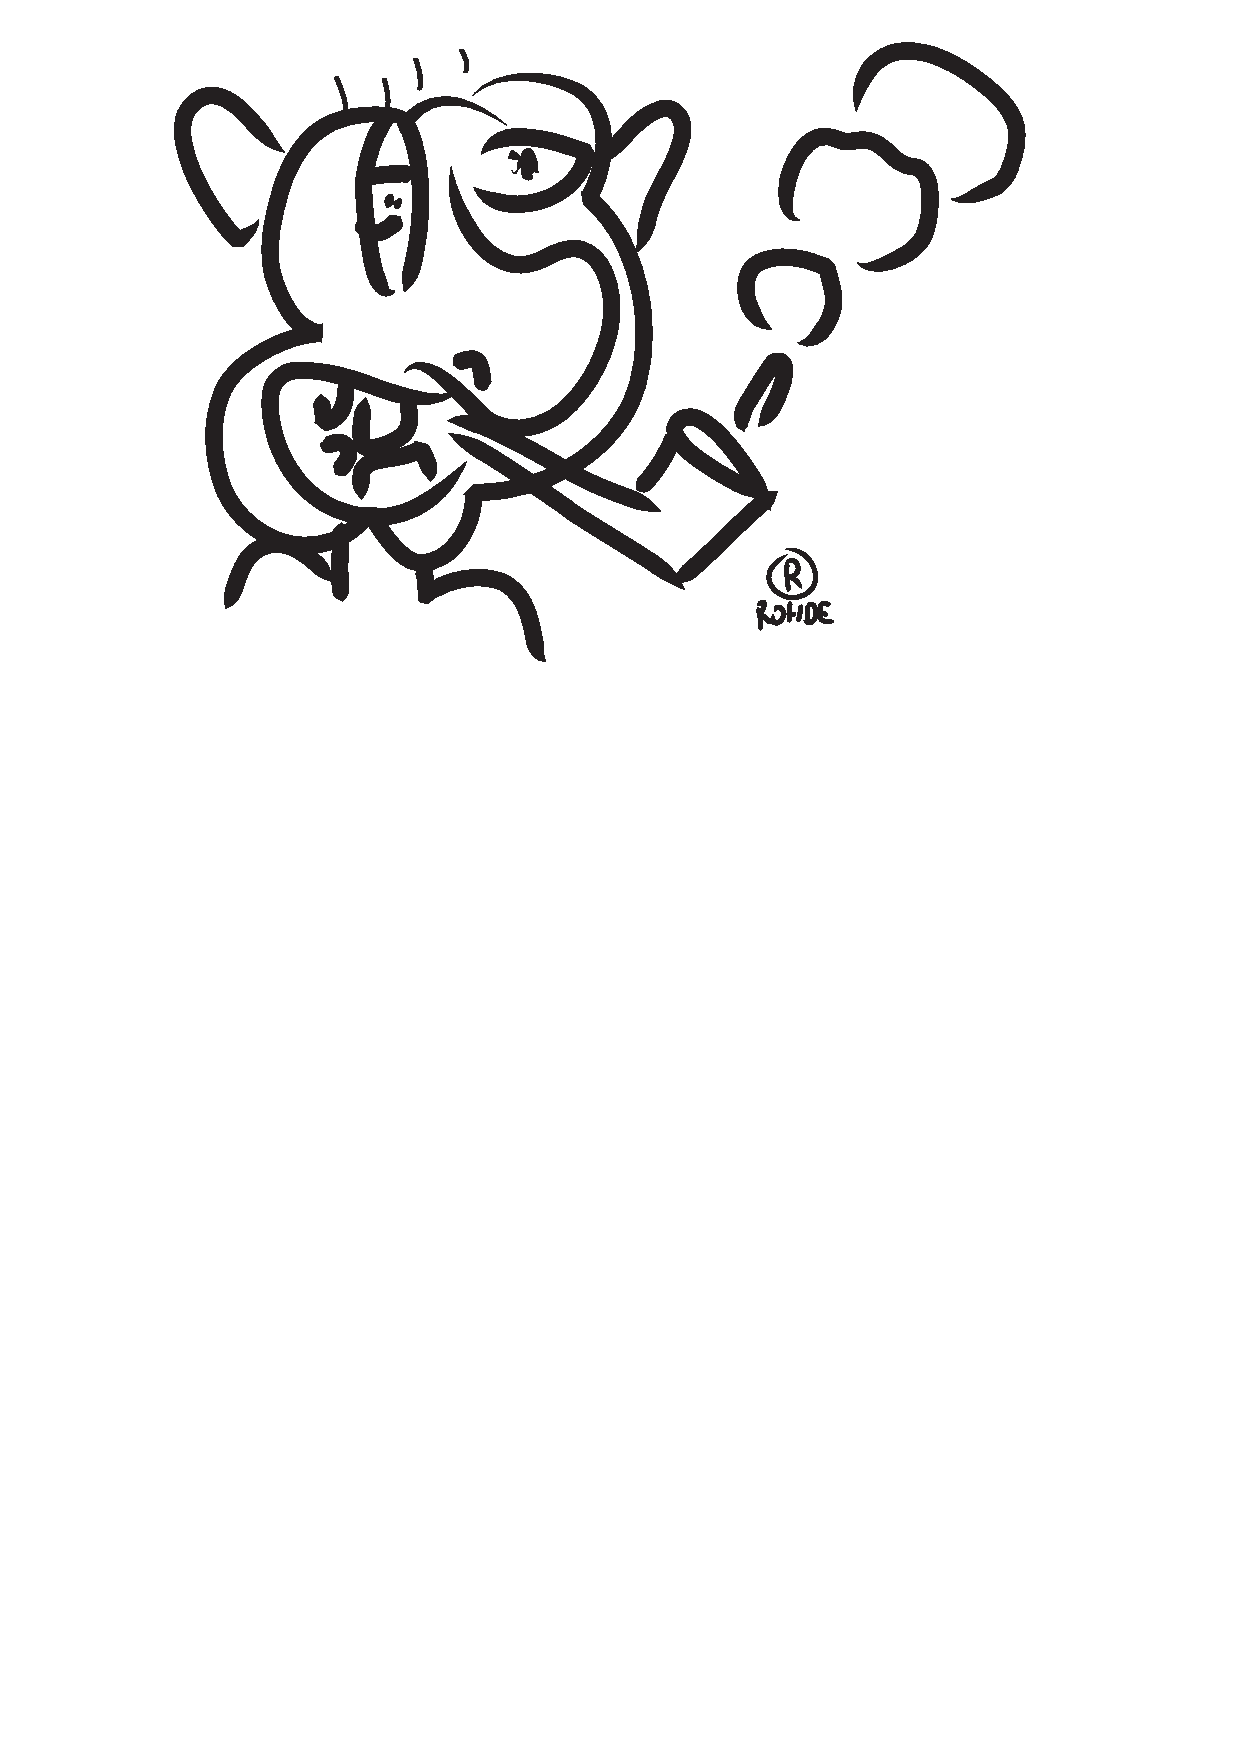
\includegraphics[width=0.55\linewidth]{sketch_cover}
\fi

\newpage
\end{abstract}

\maketitle

%
% Dedication
%

\if 1\pubmode
	\onecolumngrid
\fi

\vspace*{180px}
\begin{center}
\textit{--- To the giants upon whose shoulders we stand.}
\end{center}
\newpage

\if 1\pubmode
	\twocolumngrid
\fi


%
% Table of Contents
%

\if 1\parainTOC
	\makeatletter
	\def\l@paragraph{\@dottedtocline{4}{8em}{1.2em}}
	\makeatother
\fi

\makeatletter
\addtocontents{toc}{\def\string\@dotsep{100}}
\makeatother

\tableofcontents 
\addtocontents{toc}{~\hfill\textbf{Page}\par}

%
% Introduction
%

\part{Introduction}\label{part:introduction}\index{Introduction}

\famousquote{Any sufficiently advanced technology is indistinguishable from magic.}{Arthur C. Clarke}
\newline \newline
\famousquote{There may be babblers, wholly ignorant of mathematics, who dare to condemn my hypothesis, upon the authority of some part of the Bible twisted to suit their purpose. I value them not, and scorn their unfounded judgement.}{Nicolaus Copernicus}\index{Grandad}\index{Mansplaining}
\newline \newline
\famousquote{Imagination is more important than knowledge.}{Albert Einstein}

\if 1\pubmode
\else
	\section{Mission statement}\index{Mission statement}

\dropcap{T}{he} biological evolution of the human race is reaching a plateau. The only mechanism for us to advance further is via technology. The 20th century was that of the transistor, gifting us unprecedented progress as a species, on an exponential trajectory. However, that trajectory is rapidly approaching saturation. The 21st century will usher in entirely new technologies, far beyond just incremental developments in our current ones. Quantum technology will be one of them, transforming the world as profoundly as the transistor did. Our mission is to contribute to the realisation of this, propelling the human race into the future, benefiting all of humanity, blind to demographics and national borders. Together we will make the future.

\latinquote{Docendo discimus.}
\fi

%
% Foreword
%

\famousquote{Any sufficiently advanced technology is indistinguishable from magic.}{Arthur C. Clarke}
\newline \newline
\famousquote{There may be babblers, wholly ignorant of mathematics, who dare to condemn my hypothesis, upon the authority of some part of the Bible twisted to suit their purpose. I value them not, and scorn their unfounded judgment.}{Nicolaus Copernicus}
\newline \newline
\famousquote{Imagination is more important than knowledge.}{Albert Einstein}

\section{Foreword}\label{sec:foreword}

\dropcap{Q}{uantum} technologies\index{Quantum technologies} are not just of interest to quantum physicists, but will have transformative effects across countless areas -- the next technological revolution. For this reason, this work is directed at a general audience of not only quantum computer scientists, but also classical computer scientists, physicists, economists, artists, musicians, and computer, software and network engineers. More broadly, we hope this work will be of interest to those who recognise the future significance of quantum technologies, and the implications (or even just curiosities) that globally networking them might have -- the creation of the global quantum internet \cite{bib:van2014quantum, bib:Kimble2008}. We expect the answer to that question will look very different to what emerged from the classical internet.

A basic understanding of quantum mechanics \cite{bib:Sakurai94}, quantum optics \cite{bib:GerryKnight05}, quantum computing and quantum information theory \cite{bib:NielsenChuang00}\footnote{Throughout this manuscript we use the Nielsen \& Chuang convention for the pronunciation of `zed' \cite{bib:NielsenChuang00}.\index{Zed}}, and classical networking \cite{bib:TanenbaumNet} are helpful, but not essential, to following our discussion. Some mathematical sections require a basic understanding of the mathematical notation of quantum mechanics. Although the reader without this background ought to be able to nonetheless follow the broader arguments.

The entirely technically disinterested or mathematically incompetent reader may refer to just Parts~\ref{part:introduction}, \ref{part:essays} \& \ref{part:the_end} -- essentially brief non-technical, highly speculative essays about the motivation, applications and implications of the future quantum internet.

This work is partially a review of existing knowledge relevant to quantum networking, and partially original ideas, to a large extent based on the adaptation of classical networking concepts and quantum information theory to the context of quantum networking. A reader with an existing background in these areas could calmly skip the respective review sections.

Our goal is to present a broadly accessible technical and non-technical overview of how we foresee quantum technologies to operate in the era of quantum globalisation, and the exciting possibilities and emergent phenomena that will evolve from it.

The theme music for this work may be found at \href{http://soundcloud.com/peter-rohde/wir-sind-ein-volk}{http://soundcloud.com/peter-rohde/wir-sind-ein-volk} \copyright\index{Theme music}\footnote{We use the copyright (\copyright) and trademark (\texttrademark) symbols liberally throughout this text when referring to things where we believe commercial opportunities may exist in the future. The authors do not own copyrights or trademarks to anything in this text.}.
\sketch{sketch_1}

\latinquote{Liber magnus est.}

%
% Introduction
%

\section{Introduction} \label{sec:introduction}

The internet is one of the key technological achievements of the 20th century, an enabling factor in every aspect of our everyday use of modern technology. While digital computing was the definitive technology of the 20th century, quantum technologies will be for the 21st \cite{bib:NielsenChuang00, bib:Bennett00}. 

Perhaps the most exciting prospect in the quantum age is the development of quantum computers\index{Quantum computing}. Richard Feynman \cite{bib:Feynman85} was the first to ask the question `If quantum systems are so exponentially complex that we are unable to simulate them on our classical computers, can those same quantum systems be exploited in a controlled way to exponentially outperform our classical computers?'\index{Richard Feynman}. Subsequently, the Deutsch-Jozsa algorithm \cite{bib:DeutschJozsa92}\index{Deutsch-Jozsa algorithm} demonstrated for the first time that algorithms can run on a quantum computer, exponentially outperforming any classical algorithm. Since then, an enormous amount of research has been dedicated to finding new quantum algorithms, and the search has indeed been a very fruitful one\footnote{See the Quantum Algorithm Zoo for a comprehensive summary of the current state of knowledge on quantum algorithms (\texttt{\href{http://math.nist.gov/quantum/zoo/}{http://math.nist.gov/quantum/zoo/}}).}, with many important applications having been found, including, amongst many others\index{Quantum algorithms}:

\begin{itemize}
	\item Searching unstructured databases:\index{Grover's algorithm}
		\begin{itemize}
		\item Grover's algorithm \cite{bib:Grover96}.
		\item Quadratic speedup.
		\end{itemize}
	\item Satisfiability problems\footnote{A satisfiability problem is one where we search a function's input space for a solution(s) satisfying a given output constraint. The hardest such problems, like the archetypal \textsc{3-SAT}\index{3-\textsc{SAT}} problem, are \textbf{NP}-complete.}\index{\textbf{NP} \& \textbf{NP}-complete}:
		\begin{itemize}
			\item Grover's algorithm.
			\item Quadratic speedup.
			\item Includes solving \textbf{NP}-complete problems, and brute-force cracking of private encryption keys\footnote{Note that when performing a brute-force attack against a private encryption key\index{Private-key encryption}, a quadratic speedup effectively halves the key length in terms of algorithmic runtime. Thus, in the quantum era private key lengths will need to be doubled.}.\index{Satisfiability problems}
			\end{itemize}
	\item Optimisation problems:
		\begin{itemize}
			\item Grover's algorithm.
			\item Quadratic speedup.
			\item Many optimisation problems are \textbf{NP}-complete or can be approximated in \textbf{NP}-complete.\index{Optimisation problems}
			\end{itemize}
	\item Period finding and integer factorisation\index{Shor's algorithm}:
		\begin{itemize}
		\item Shor's algorithm \cite{bib:ShorFactor}.
		\item Exponential speedup.
		\item This compromises Rivest, Shamir \& Adleman (RSA) public-key cryptography \cite{bib:RSA}\index{RSA encryption}\index{Public-key encryption}, the most widely used cryptographic protocol on the internet today.
		\end{itemize}
	\item Simulation of quantum systems\index{Quantum simulation}:
		\begin{itemize}
			\item Lloyd's algorithm \cite{bib:lloyd1996universal}.
			\item Exponential speedup.
			\item This includes simulation of: molecular and atomic interactions in the study of quantum chemistry or nuclear physics; interactions between drug molecules and organic molecules for drug design; genetic interactions for the study of genetics and genetic medicine; nanoscale semiconductor physics for integrated circuit design; and much more.
			\end{itemize}
	\item Simulation of quantum field theories\index{Simulating quantum field theories}:
		\begin{itemize}
		 \item Jordan-Lee-Preskill algorithm \cite{bib:JLP, bib:RohdeWavelet15}
		 \item Exponential speedup.
		 \item A key area of fundamental physics research.
		 \end{itemize}
	\item Topological big-data analysis:\index{Topological big-data analysis}
		\begin{itemize}
		\item Lloyd's algorthm \cite{bib:lloyd2016quantum, USTCexperiment}.
		\item Exponential speedup.
		\item Broad applications including: social media network analysis; consumer behaviour; behavioural dynamics; neuroscience; and higher-dimensional signal and image processing.
		\end{itemize}
	\item Solving linear systems of equations:\index{Linear systems}
		\begin{itemize}
		\item \comment{To do} \cite{bib:harrow2009quantum, bib:BerryLinear}.
		\item Exponential speedup.
		\item Widespread applications in linear algebra and calculus.
		\end{itemize}
	\item Quantum machine learning:\index{Quantum machine learning}
		\begin{itemize}
		\item Lloyd's algorithm \cite{bib:lloyd2013quantum}.
		\item This includes putting an end to humanity.
		\item \textit{Ne obliviscaris}.
		\end{itemize}
\end{itemize}
An elementary technical overview of some of these archetypal algorithms is presented in Sec.~\ref{sec:quantum_algs}.

It is likely we haven't yet begun to fully recognise the capabilities of quantum computers, and the full plethora of applications they may have in the future. We stand at the beginning of the emergence of an entirely new type of technology.

In addition to many practical applications, the onset of quantum computing carries with it deep philosophical implications. Specifically, the Extended Church-Turing (ECT)\index{Extended Church-Turing (ECT) thesis} thesis hypothesises that any physically realisable system can be \textit{efficiently}\footnote{The term `efficient' is one coined by the computer scientist to mean that a problem can be solved in time at most polynomial in the size of the problem.\index{Computational efficiency}} simulated by a universal Turing machine\index{Turing machines} (i.e classical computer). The believed exponential complexity of quantum systems inclines quantum computer scientists to believe that the ECT thesis is therefore false \cite{bib:Deutsch85}\footnote{We have discovered a truly marvelous proof of this, which this footnote is too narrow to contain.}. The demonstration of large-scale quantum computers, while unable to prove or disprove the ECT thesis\footnote{When one talks about `scalability' or the `ECT thesis', we are talking about asymptotic relationships. Clearly no finite-sized experiment can prove asymptotic scaling with certainty. But with a sufficiently large quantum computer at our disposal, demonstrating exponentially more computational power than its classical sibling, we might be reasonably satisfied in convincing ourselves about the nature of the scaling of different computational models.}, could at least provide some convincing evidence against the ECT conjecture.

From a computational complexity\index{Computational complexity theory} theorist's perspective, it is strongly believed that the complexity classes of problems efficiently solvable on classical computers (\textbf{P} \& \textbf{BPP}\index{\textbf{P} \& \textbf{BPP}}) and quantum computers (\textbf{BQP}\index{\textbf{BQP} \& \textbf{BQP}-complete}) are distinct. Specifically, it is believed that \mbox{$\mathbf{BPP}\subset\mathbf{BQP}$}. If this conjecture is correct, it implies the existence of quantum algorithms super-polynomially faster than the best classical ones, and that the ECT thesis is not correct. More specifically, Fig.~\ref{fig:complexity_classes} illustrates the believed relationships between some of the most important complexity classes relevant to quantum computing.

\begin{figure}[!htb]
	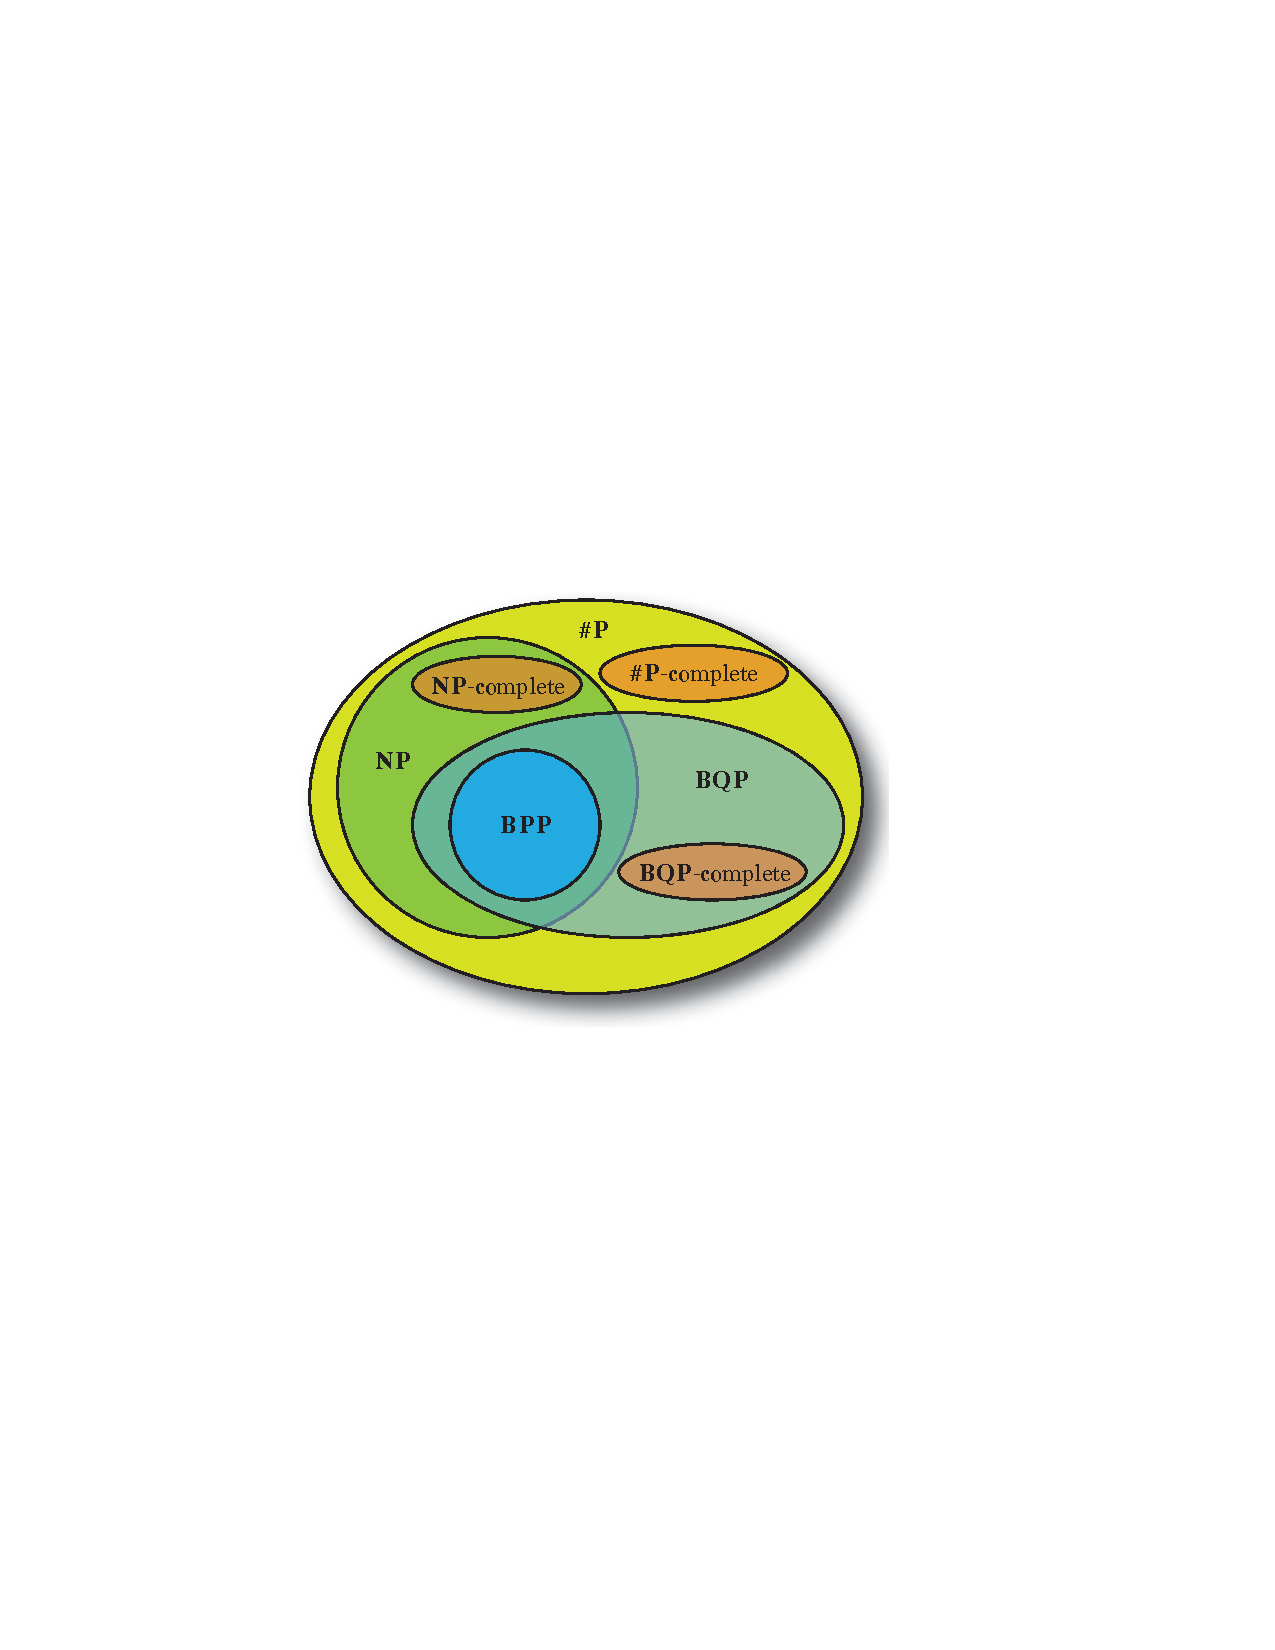
\includegraphics[width=\columnwidth]{complexity_classes}\index{Complexity classes} \index{\textbf{P} \& \textbf{BPP}} \index{\textbf{NP} \& \textbf{NP}-complete} \index{\textbf{BQP} \& \textbf{BQP}-complete} \index{\textbf{\#P} \& \textbf{\#P}-complete}
	\caption{Believed relationships between the complexity classes most relevant to quantum computing. \textbf{BPP} is the class of polynomial-time probabilistic classical algorithms. \textbf{NP} is the class of problems verifiable in polynomial time using classical algorithms. \textbf{NP}-complete are the subset of \textbf{NP} problems polynomial-time reducible to any other problem in \textbf{NP}. \textbf{BQP} is the class of probabilistic algorithms solvable in polynomial time on universal quantum computers. $\#\mathbf{P}$ is the set of counting problems, that count satisfying solutions to \textbf{P} problems (\textbf{P} is the same as \textbf{BPP}, but deterministic, rather than probabilisitic). Note that it is actually unproven whether \mbox{$\mathbf{P}=\mathbf{BPP}$} or \mbox{$\mathbf{P}\subset\mathbf{BPP}$}. There are examples where the best known \textbf{BPP} algorithms outperform the best known \textbf{P} algorithms, which could arise because the two classes are inequivalent, or that we simply haven't tried hard enough to find the best deterministic algorithms. Furthermore, while it is known that \mbox{$\mathbf{P}\subseteq\mathbf{NP}$}, it is not known whether \mbox{$\mathbf{BPP}\subseteq\mathbf{NP}$}. For the sake of illustration in our Venn diagram we have taken the view that it is. \textbf{BPP} is regarded as the class of problems efficiently solvable on universal Turing machines (i.e classical computers), whereas \textbf{BQP} is that efficiently solvable on universal quantum computers. The computational superiority of quantum computers is based on the (strongly believed, yet unproven) assumption that \mbox{$\mathbf{BPP}\subset\mathbf{BQP}$}.} \label{fig:complexity_classes}
\end{figure}

Aside from quantum computing, quantum cryptography\index{Quantum cryptography} holds the promise of uncrackable cryptographic protocols, guaranteed not by the assumed complexity of solving certain mathematical problems like integer factorisation or brute-force searching, but by the laws of quantum mechanics. That is, provided our understanding of quantum mechanics is correct, quantum cryptographic protocols exist, which cannot be cracked, irrespective of the computational resources of an adversary.

Already we are beginning to see elementary realisations of essential quantum technologies such as quantum computing, cryptography, and metrology. As these technologies become increasingly viable and more ubiquitous, the demand for networking them and sharing quantum resources between them will become a pressing issue. Most notably, quantum cryptography and \textit{cloud quantum computing} will be pivotal in the proliferation of quantum technology, which necessarily requires reliable quantum communications channels.

The first demonstrations of digital computer networks were nothing more than simple two-party, point-to-point (P2P) communication. However, the internet we have today extends far beyond this, allowing essentially arbitrary worldwide networking across completely ad hoc networks comprising many different mediums, with any number of parties, in an entirely plug-and-play and decentralised fashion. Similarly, elementary demonstrations of quantum communication\index{Quantum communication} have been performed across a small number of parties, and much work has been done on analysing quantum channel capacities in this context \cite{??? channel_capacity}. But, as with digital computing, demand for a future \textit{quantum internet} is foreseeable, enabling the arbitrary communication of quantum resources, between any number of parties, over ad hoc networks.

The digital internet may be considered a technology stack, such as TCP/IP (Transmission Control Protocol/Internet Protocol)\index{Transmission Control Protocol/Internet Protocol (TCP/IP)}, comprising different levels of abstraction of digital information \cite{bib:TanenbaumNet}. At the lowest level we have raw digital data we wish to communicate across a physical medium. Above this, we decompose the data into packets. The packets are transmitted over a network, and TCP is responsible for routing the packets to their destination, and guaranteeing data integrity and Quality of Service (\textsc{QoS}). Finally, the packets received by the recipient are combined and the raw data reconstructed.

The TCP layer remains largely transparent to the end-user, enabling virtual software interfaces to remote digital assets that behave as though they were local. This allows high-level services such as the File Transfer Protocol (FTP), the worldwide web, video and audio streaming, and outsourced computation on supercomputers, as though everything was taking place locally, with the end-user oblivious to the underlying networking protocols, which have been abstracted away. To the user, YouTube videos or Spotify tracks behave as though they were held as local copies. And FTP or DropBox allow storage on a distant data centre to be mounted as though it were a local volume. We foresee a demand for these same criteria in the quantum era.

In the context of a quantum internet, packets of data will instead be quantum states, and the transmission control protocol is responsible for guiding them to their destination and ensuring quality control.

Here we present a treatment for such Quantum Transmission Control Protocols (QTCPs)\index{Quantum Transmission Control Protocol (QTCP)} as a theoretical foundation for a future quantum internet. We consider how such ad hoc networks may be described mathematically, how to quantify network performance, and present a QTCP stack for operating it. While the goals of QTCP are similar as for classical TCP, there are major conceptual differences between the classical and quantum internets, owing to the unique properties of quantum states with no classical analogue.

Our treatment of quantum networks will be optics-heavy, based on the reasonable assumption that communications channels will almost certainly be optical, albeit with many possible choices of optical states and mediums. However, this does not preclude non-optical systems from representing quantum information that is not in transit, and we consider such `hybrid' architectures in detail, as well as the interfacing between optical and non-optical systems. Indeed, it is almost certain that future large-scale quantum computers will not be all-optical, necessitating interfacing different physical architectures. We accommodate for this requirement in the design of the QTCP.

Shared quantum entanglement\index{Quantum entanglement} is a primitive resource with direct applications in countless protocols. This warrants special treatment of quantum networks, which do not implement a full QTCP network stack, but instead specialise in just this one task -- entanglement distribution. We will see that such a specialised network will already be immensely useful for a broad range of applications, and its simplicity brings with it many inherent advantages.

The quantum internet will enable advances in the large-scale deployment of quantum technologies. Most notably, in the context of quantum computing it will allow initially very expensive technology to be economically viable and broadly accessible via the outsourcing of computations from consumers who can't afford quantum computers, to well-resourced hosts who can -- \textit{cloud quantum computing}\index{Cloud quantum computing}.

With the addition of recent advances in homomorphic encryption and blind quantum computing\index{Encrypted quantum computation}, such cloud quantum computing can be performed securely, guaranteeing privacy of both data and algorithms, secure even against the host performing the computation. This opens up entirely new economic models and applications for the licensing of compute time on future quantum computers in the cloud.

The unique behaviour of quantum computing, in terms of the super-classical scaling in its computational power, brings with it many important economic and strategic considerations that are extremely important to give attention to in the post-classical world.

But quantum technologies extend far beyond computation. Many other exciting applications for controlled quantum systems exist, with new ones frequently emerging. Thus, the quantum internet will find utility beyond cloud quantum computing, enabling the global exchange of quantum resources and assets. This could include the networking of elementary quantum resources such as state preparation, entanglement sharing, teleportation and quantum measurements, or scale all the way up to massively distributed quantum computation or a global quantum cryptography network.\index{Quantum assets}

It is hard to foresee the future trajectory of quantum technology, much as no one foresaw the advances digital technology has made over the last half century. But it is certain that as the internet transformed digital technology, the quantum internet will define the future of quantum technologies.
\sketch{sketch_4}

\latinquote{Vincit qui se vincit.}

%
% Classical networks
%

\part{Classical networks}\label{part:class_net}\index{Classical networks}

%
% Classical Networking Protocols
%

\section{Classical networking protocols} \label{sec:classical_nets} \index{Classical networking protocols}

\dropcap{T}{o} set the context for our upcoming treatment of quantum networks, we begin by discussing \textit{classical} networks, and some of the key protocols behind their operation.

There have been numerous approaches employed in the past for sharing communications links between multiple users\index{Shared communication channels}. This includes:
\begin{itemize}
	\item Channel-switching: an entire communications channel is designated for exclusive use by a given user. \index{Channel-switched networks}
	\item Packet-switching: data is divided into packets, which are routed independently by the network, being reconstructed by the recipient once all packets have been received.\index{Packet-switching}
	\item Time- or frequency-multiplexing: each user is designated a particular frequency spectrum or series of time-slots exclusively for their use. \index{Time-multiplexing}\index{Frequency-multiplexing}
	\item Code Division Multiple Access (CDMA): all users can broadcast over a channel simultaneously, and the construction of the coding technique enables demultiplexing of the distinct signals, despite their interference with one another.\index{Code Division Multiple Access (CDMA)}
	\item Ethernet: all users are free to broadcast\index{Broadcast networks} over a shared channel at will, and \textit{collision detection}\index{Collision detection} identifies when packets interfere, after which they are discarded and rebroadcast following a random waiting period, repeating until success.\index{Ethernet}
\end{itemize}

Nowadays packet-switched networks have become the norm in most digital networks, as they facilitate far greater efficiency in the use of network bandwidth, and are more easily scaled to greater numbers of users in a dynamic and ad hoc manner. It is foreseeable the same trend will continue with quantum technologies, especially given their initial high cost, where maximising network utility is paramount.

In this work we will focus on packet-switched networks when we later introduce our quantum networking protocols. However, with sufficient flexibility in the design of our upcoming quantum protocols, packet-switched networks can easily be made to effectively implement channel-switched, or time-/frequency-multiplexed communication.

%
% TCP/IP
%

\subsection{TCP/IP} \index{Transmission Control Protocol/Internet Protocol (TCP/IP)}

The present-day internet is built on top of a protocol stack comprising primarily the Internet Protocol (IP), User Datagram Protocol (UDP), and Transmission Control Protocol (TCP). Most commonly, these are simply referred to as TCP/IP. These define a stack of different layers of abstraction for communicating data packets between nodes in a network, determining their routing, and enforcing any quality of service requirements.

%
% Internet Protocol
%

\subsubsection{Internet Protocol} \index{Internet Protocol (IP)}

IP is the standard protocol employed in the internet for P2P communication of data packets. It is a low-level protocol that encapsulates digital data into packets containing a header field, which specifies routing information, most notably the IP addresses of the source and destination. IP does not enforce any kind of quality control, which is instead delegated to higher-level protocols like TCP (Sec.~\ref{sec:TCP}), a higher-level of abstraction built on top of IP (Sec.~\ref{sec:TCP}).

Multiple packets with the same source and destination needn't follow the same route -- the routing is determined dynamically in realtime by routers, based on network characteristics such as load or latency. Thus, packets belonging to the same underlying data may arrive out of order, or some may go missing altogether. IP does not address these issues, instead engaging in only `best-effort' delivery. 

In IP there is no central authority with knowledge of the state of the entire network, which tells routers in the network how to best route packets. Thus, IP must be complemented with up-to-date routing tables, held by routers/nodes in the network, which make routing decisions on a per-packet basis. This is achieved using gateway protocols, discussed next.

%
% User Datagram Protocol
%

\subsubsection{User Datagram Protocol} \index{User Datagram Protocol}

The UDP is a simple protocol built on top of IP, based on a `send-and-forget' principle for sending data packets. That is, there is no quality of service guarantee, and no notifications are provided to the sender as to whether packets successfully reached their destination. However, a checksum (hash) forms a part of the packet headers to enable error detection by the recipient. The lack of quality control bypasses the associated latency, making it particularly useful in time-critical applications, where the late arrival of a packet is useless and therefore needn't be retransmitted.

UDP is connectionless, meaning that no designated connection is established between hosts. Instead data is simply transmitted and then forgotten about. The receiver may not even be operational on the network, in which case the packets are lost without notice.

Key examples for the use of UDP are realtime audio and video transmission. If a packet associated with a frame in a video link is delayed and arrives several frames late, it is useless, since it is associated strictly with a previous frame in the video that has already passed. Quality control, in the form of contacting the sender to request a retransmission, would therefore achieve nothing. This applies similarly to live audio streaming, such as voice over IP (VoIP)\index{Voice over IP}, where the late arrival of a packet cannot possibly be correctly inserted into the audio playback and might as well be discarded.

Therefore, UDP prioritises latency over reliability, and is best suited to time-critical applications where quality of service is not relevant.

%
% Transmission Control Protocol (TCP)
%

\subsubsection{Transmission Control Protocol} \label{sec:TCP} \index{Transmission Control Protocol}

TCP differs from UDP in that it intrinsically supports quality control. The protocol is able to determine whether a packet successfully reached its destination, and if not, retransmit it as often as necessary to guarantee packet delivery. A checksum is also included in packet headers to enable error detection. This quality control has made TCP the dominant protocol employed in the present-day internet, where, in most scenarios, we wish to guarantee that data has been correctly delivered -- if an email is missing random segments of its text, users will become irate very quickly!

TCP is connection-oriented, meaning that a handshaking protocol establishes a dedicated bidirectional channel between two hosts. It also enforces packet reordering, to counter out-of-order packet arrival.

However, the enforced quality control and handshaking protocols incur a network performance overhead that UDP does not, since handshaking protocols consume bandwidth. Thus, TCP should not be used instead of UDP if there are no quality of service requirements.

%
% Ethernet
%

\subsection{Ethernet} \index{Ethernet}

Ethernet is a networking protocol based on `broadcasting' on a shared network. This model is particularly suited to local area networks (LANs), where all users share a single communications channel rather than dedicated P2P links, as shown in Fig.~\ref{fig:ethernet}.

\begin{figure}[htpb]
	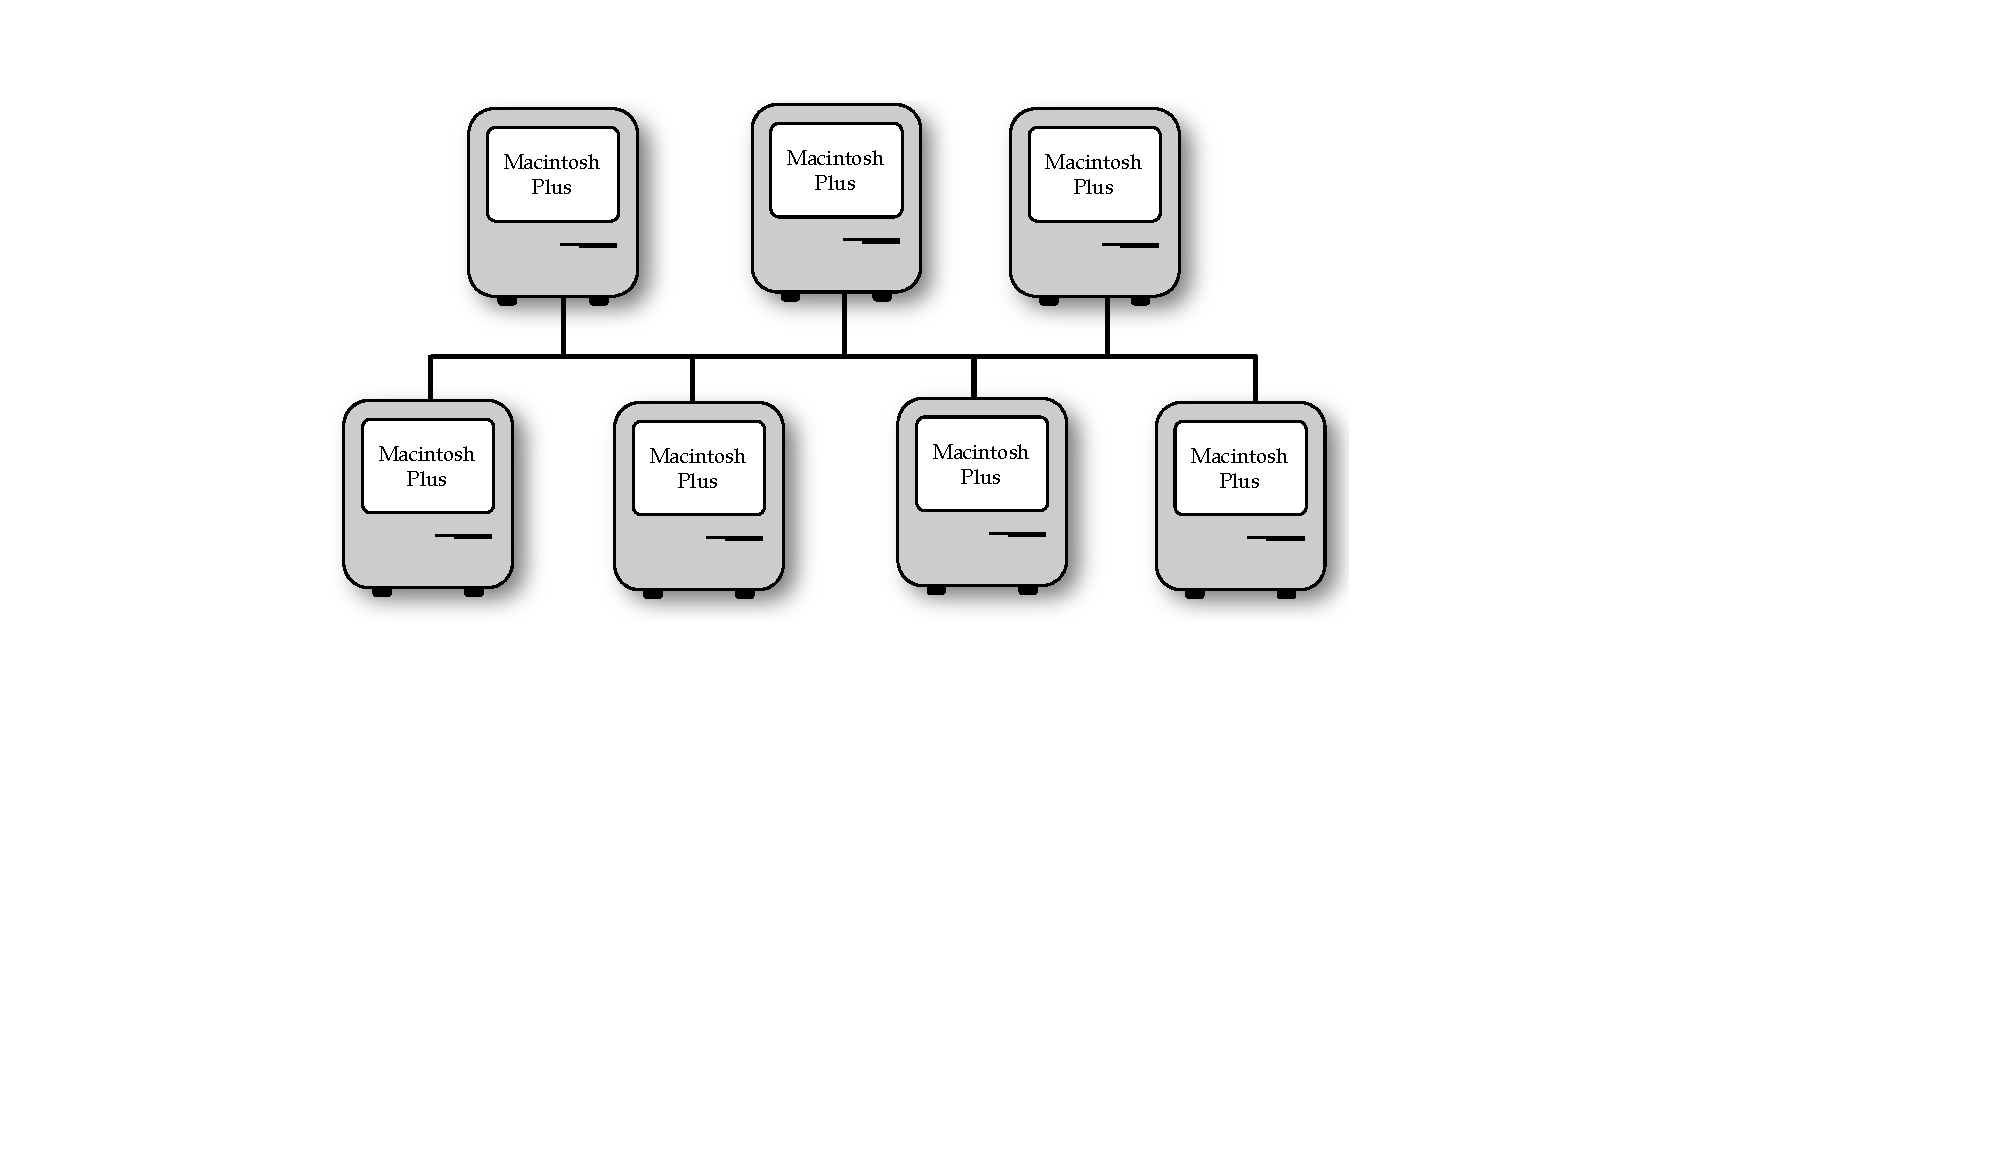
\includegraphics[width=0.47\textwidth]{ethernet}
	\caption{The topology of an Ethernet network, whereby all users share a common channel, which they can broadcast to at their leisure. If data packets collide, it is detected via the packets' checksums, and the corrupted packets may be re-broadcast after a random `backoff' waiting period, repeating this process until packet delivery is successful. Obviously the chance of collisions occurring increases with the number of connected users, thus network performance is inversely related to the number of nodes.} \label{fig:ethernet}
\end{figure}

In the Ethernet protocol, every user is free to broadcast data onto the shared channel as they please -- all users transmit to, and receive from a single shared channel. However, clearly sometimes packet `collisions' will occur\index{Collision handling}, resulting in packet corruption. To overcome this, Ethernet packets contain a checksum that can be used to verify upon arrival whether a packet has been corrupted by a collision. If a collision is detected, the respective users are able to re-broadcast, following a randomly chosen waiting period (known as `backoff')\index{Backoff}. Collisions therefore reduce network performance, and it follows that network bandwidth decreases with the number of users competing for bandwidth\footnote{Think of that awkward dinner table conversation, where two people start talking simultaneously (Peter \& Jon). It's immediately obvious to them both that they are interfering with one another, and if they were to just talk over one another (packet collision), no one would understand either of them. So, they both awkwardly pause, before starting to speak again. In a \textit{really} awkward conversation, they will both start again simultaneously, after which there will be an even longer awkward pause before recommencing. Eventually, this self-regulating system will resolve itself probabilistically, with a sole victor controlling the airwaves, commanding the attention of the listeners. Provided that all dinner guests adhere to social etiquette and backoff appropriately, with repeated conversations, all guests will statistically receive an equitable share of attention, albeit with some wastage of conversation time owing to the periods of silence. Clearly, the proportion of the time wasted due to collisions will scale up with the number of guests, limiting the protocol to not-too-large tables (or very quiet guests).}.

From this protocol, any given packet will eventually be successfully transmitted uncorrupted, collision-free, albeit with uncertain timing that grows with the number of competing users. For this reason, the Ethernet protocol is not ideal for time-critical applications requiring hard guarantees on network latency.

The beauty of this approach is that only a single channel is required for connecting all users. No dedicated P2P connections are required. As the number of users increases, the complexity of the network topology does not -- requiring only the addition of a node to the existing backbone. For small LANs this is clearly reasonably functional. However, as the size of networks increases, the rate at which packet collisions occur increases, resulting in a reduction in network bandwidth. Thus, the Ethernet protocol is ideally suited to small LANs, but is clearly not viable at a global level, where network competition is astronomical and the overhead from backoff would reduce network performance to a standstill, wasting most of the bandwidth.

Another elegant feature of the Ethernet protocol is that bandwidth allocation is self-regulating, with bandwidth fairly and equitably allocated between users, not prioritising any user over another. This applies even in completely ad hoc networks, with users joining and leaving the network willy nilly. Provided all users are correctly and honestly implementing the \textsc{Broadcast and Backoff} protocol, network bandwidth is allocated evenly amongst users, and no mediating, overriding central authority is needed to oversee network resource allocation. This allows Ethernet networks to be truly `plug-and-play'.

%
% Gateway Protocols & Routing Tables
%

\subsection{Gateway protocols \& routing tables} \label{sec:gateway} \index{Gateway protocols} \index{Routing tables}

In the absence of a central mediating authority, routing decisions must be made by individual nodes in the network, upon receipt of packets. For routers to make sensible routing decisions, they must have some idea of the overall structure and state of the network. This is achieved using gateway protocols, which communicate information about the state of the network on a nearest-neighbour basis. There are various gateway protocols in use, with the Exterior Gateway Protocol (EGP)\index{Exterior Gateway Protocol (EGP)} and Border Gateway Protocol (BGP)\index{Border Gateway Protocol (BGP)} being very common.

We let every node in the network have a routing table, initially empty, that will ultimately be populated with information on how to best route incoming packets further along the route to their destination.

To mitigate the need for a central authority, nodes engage in only nearest neighbour communication, sharing their routing tables with one another, to query about the distance metrics (Sec.~\ref{sec:costs}) associated with routes to different destinations. This communication is taking place regularly, and as nodes' routing tables become populated, updating in real-time, they will (hopefully) reach a steady-state. From these tables, single-source shortest path algorithms (Sec.~\ref{sec:single_source_sp}) can be applied by nodes to construct a complete picture of costs to every point in the network. Such a nearest neighbour algorithm is effectively a distributed breadth-first-search\index{Breadth-first-search (BFS) algorithm} algorithm (Sec.~\ref{sec:path_exp}).

%
% Network Hierarchies
%

\subsection{Network hierarchies} \index{Network hierarchies}

The disadvantage of Ethernet's \textsc{Broadcast and Backoff} principle is that packets are often wasted -- whenever a collision occurs. Because there is no mediating central authority, packet collisions are a certainty in a heavily-utilised shared network, each time resulting in packet loss, and an associated reduction in usable network bandwidth.

To the other extreme, we could have dedicated P2P channels between every pair of users. Then there would be guaranteed no packet collisions, and therefore maximum bandwidth efficiency, but the network would be extremely costly, and plug-and-play extremely challenging.

To address this dilemma, the topology and subdivision of networks need to be carefully designed. If we consider a large organisation, for example, potentially networking thousands of desktop PCs, the bandwidth wastage associated with packet collisions could grind the entire network to a halt, were all thousands of PCs to be communicating large amounts of data simultaneously. However, if a hierarchy of subnetworks could be implemented, rather than a single monolithic network, efficiency could be improved drastically.

Suppose our hypothetical organisation had several different departments, and users had a tendency to communicate primarily with other users in the same department. By defining distinct departmental subnets, which individually implement Ethernet, but interconnect with one another using an alternate routing framework, we can easily see that many unnecessary packet collisions may be entirely avoided. That is, why broadcast data to users who we know don't want it? A simple example of this is shown in Fig.~\ref{fig:net_hierarchy}.

\begin{figure}[htpb]
	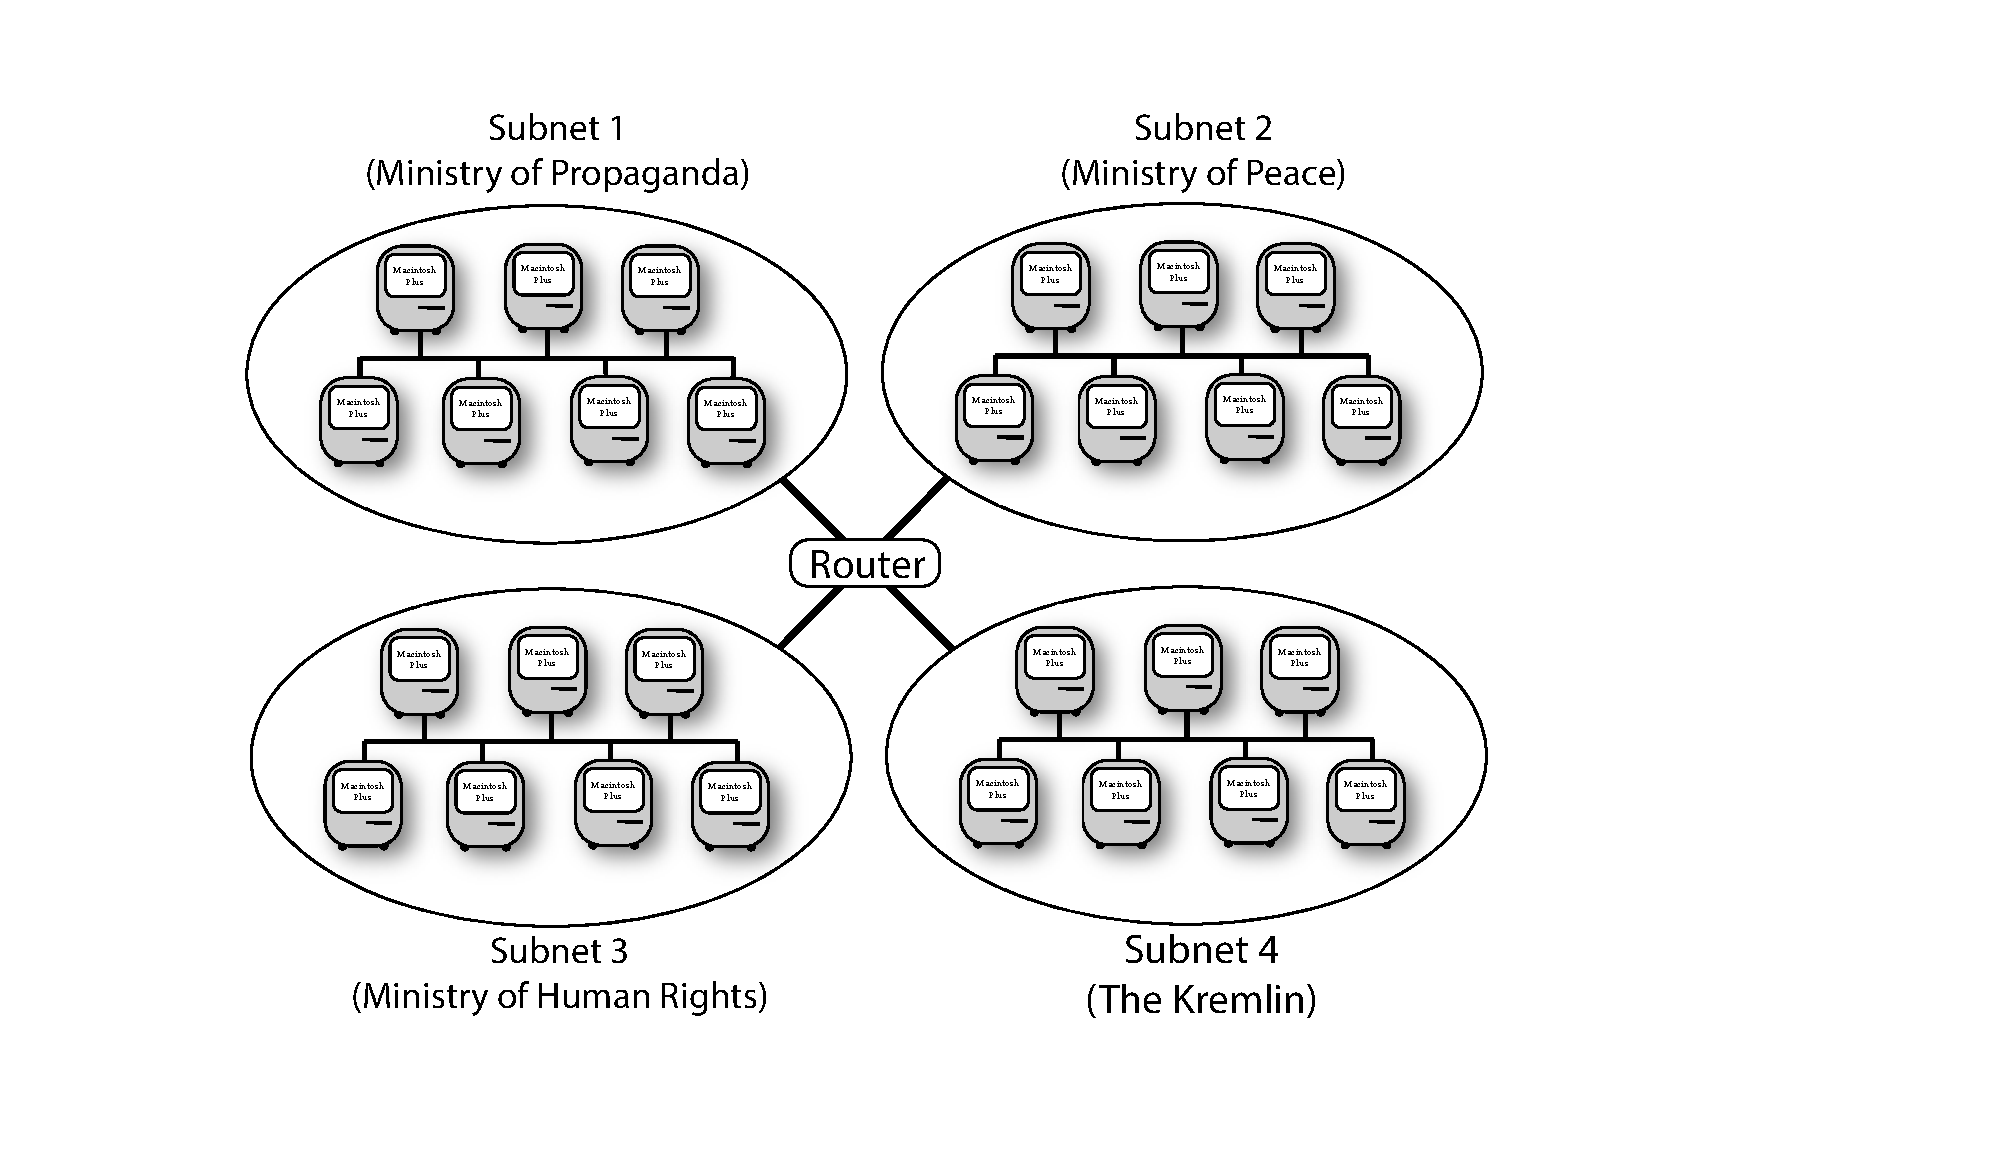
\includegraphics[width=0.47\textwidth]{network_hierarchy}
	\caption{Simple example of a network with two levels in its hierarchy. At the lowest level are 4 different subnets belonging to different departments within an organisation, each of which implements Ethernet networking. Above this, the subnets connect together in a star network via a central router. By subdividing the network hierarchy as such, if most traffic emanating within a subnet stays within that same subnet, collisions between packets on different subnets are avoided, thereby improving the efficiency of the subnets' Ethernet implementations.} \label{fig:net_hierarchy}
\end{figure}

Extending upon this simple intuitive example, enormous amounts of research and development have been invested into the design of network hierarchies, and how to optimise their efficiency. A pressing consideration in the design of network protocol stacks is therefore to accommodate for multiple routing protocols, and enabling their inter-compatibility.
\sketch{sketch_7}

\latinquote{Te futueo et caballum tuum.}

%
% Mathematical Representation of Networks
%

\section{Mathematical representation of networks}

We now turn our attention to defining a mathematical construction for the representation of (quantum and/or classical) networks, that we will subsequently rely on heavily in our framework for quantum networks. This encompasses representing networks as graphs, representing the cost of communications within the network, and how to optimise network routing to minimise costs.  These notions will be essential in our treatment of quantum networks.

%
% Graph-Theoretic Representation
%

\subsection{Graph-theoretic representation} \index{Network graphs}

We consider a classical network to be a weighted, directed graph,
\begin{align}\index{Network graph}
	G=(V,E),
\end{align}
where vertices represent \textit{nodes} (\mbox{$v\in V$}) in the network, and the weighted edges represent communication \textit{links} (\mbox{$e\in E$}) between neighbouring nodes \cite{???}.

A node could be, for example, data storage, a classical computer implementing a computation, a router that switches the connections between incoming and outgoing links, or an end-user -- anything that communicates with the network, sender or receiver. A link on the other hand is any arbitrary means of communication between nodes, such as optical fibre, satellite, radio, electrical, smoke signals, tin cans connected by a taut piece of string, or well-trained carrier pigeon. In the protocols to be described here, it is completely irrelevant what the specific mediums for communication are. Rather what matters are \textit{costs} and \textit{attributes}, quantifying the relative performance of different links.

A key feature of the global internet is redundancy. In a packet-switched environment, sending identical packets twice might each follow entirely different routes to their common destination. Node-to-node redundancy is easily accommodated for in the graph-theoretic model by allowing multiple distinct edges between nodes. It is extremely important to accommodate multiple edges in network graphs, since redundant routes provide a direct means by which to load-balance a route. So, for example, a hub in Australia might connect to a sister hub in New Zealand using both a fibre-optic undersea cable, and simultaneously via a satellite uplink. If the faster of the two connections is running out of capacity, a proportion of the packets can simply be switched to the other link, thereby balancing the load. For this reason we abstain from using an adjacency matrix representation for network graphs, as they do not accommodate redundancy.

%
% Cost Vector Analysis
%

\subsection{Cost vector analysis} \label{sec:costs} \index{Cost vectors}\index{Attributes}

The edge weights in $G$ represent the \textit{costs} ($\vec c$) and \textit{attributes} ($\vec a$) associated with using that link. In general these needn't be single numbers, but would rather be sets or data-structures, representing different types of costs and attributes of links, of which there may be many. These could include, for example, latency, bandwidth, dollar cost, and quality measures.

The distinction between costs and attributes, is that costs may be expressed in terms of units which may be interpreted as distances metrics in a Euclidean sense, obeying the following requirements:

\begin{definition}[Network cost metrics] \label{def:metric} Cost metrics satisfy the properties:\index{Network cost metrics}
	\begin{itemize}
    	\item Identity operations: If a channel performs nothing, its associated cost is zero, \mbox{$c(\mathbb{\hat{I}}) = 0$}.
    	\item Triangle inequality: \\ $c(v_1\to v_2\to v_3) \leq c(v_1\to v_2) + c(v_2\to v_3)$, \\ across all paths \mbox{$v_1 \to v_2 \to v_3$}. In the case of strict equality under addition we refer to the cost as a \emph{strictly additive cost}.
    	\item Positivity: \mbox{$c\geq 0$}. This ensures that shortest-path algorithms will function correctly. It is also congruent with the intuitive expectation that data traversing a communications channel is not somehow better off than if it hadn't traversed that channel at all.
	\end{itemize}
\end{definition}
Attributes, on the other hand do not have a distance interpretation, and may have arbitrary structure. A detailed discussion on the relationship between costs and attributes is presented in Sec.~\ref{sec:c_vs_a}.

The reason we demand costs have a distance interpretation is so that graph-theoretic pathfinding algorithms (Sec.~\ref{sec:shortest_path}) are applicable, allowing us to build upon the vast pre-existing understanding of graph theory. Ideally we would like equality in costs' triangle inequality, which yields an exact cost. But often this isn't possible and we are satisfied with the inequality, which simply dictates an upper bound on cost.

A detailed discussion of some of the major costs and attributes that realistic quantum networks will be subject to is presented in Sec.~\ref{sec:quantum_meas_cost}.

A \textit{route}\index{Routes} between two nodes, Alice ($A$) and Bob ($B$), of the network, $G$, is an acyclic subgraph connecting those nodes, \mbox{$R_{A\to B}\subseteq G$}. In general ad hoc networks there will typically be multiple paths between two nodes \mbox{$A\to B$}. For a particular cost metric, the cost of an entire route is simply the sum of the costs of each of the constituent links,
\begin{definition}[Route costs]
The net cost of a route \mbox{$A\to B$}, using cost metric $c(A\to B)$, traversing nodes $v_i$, is,
\begin{align}\index{Route costs}
c(R_{A\to B}) = \sum_{i=1}^{|R_{A\to B}|-1} c(v_i \to v_{i+1}),
\end{align}
where $v_i$ is the $i$th node in the route $R_{A\to B}$.
\end{definition}

Fig.~\ref{fig:example_routes} illustrates a simple example network with all of its available routes, \mbox{$R_{A\to B} \subseteq G$}. Fig.~\ref{fig:simp_route_opt} illustrates the optimal path for \mbox{$A\to B$} based on edge weights.

\begin{figure}[!htb]
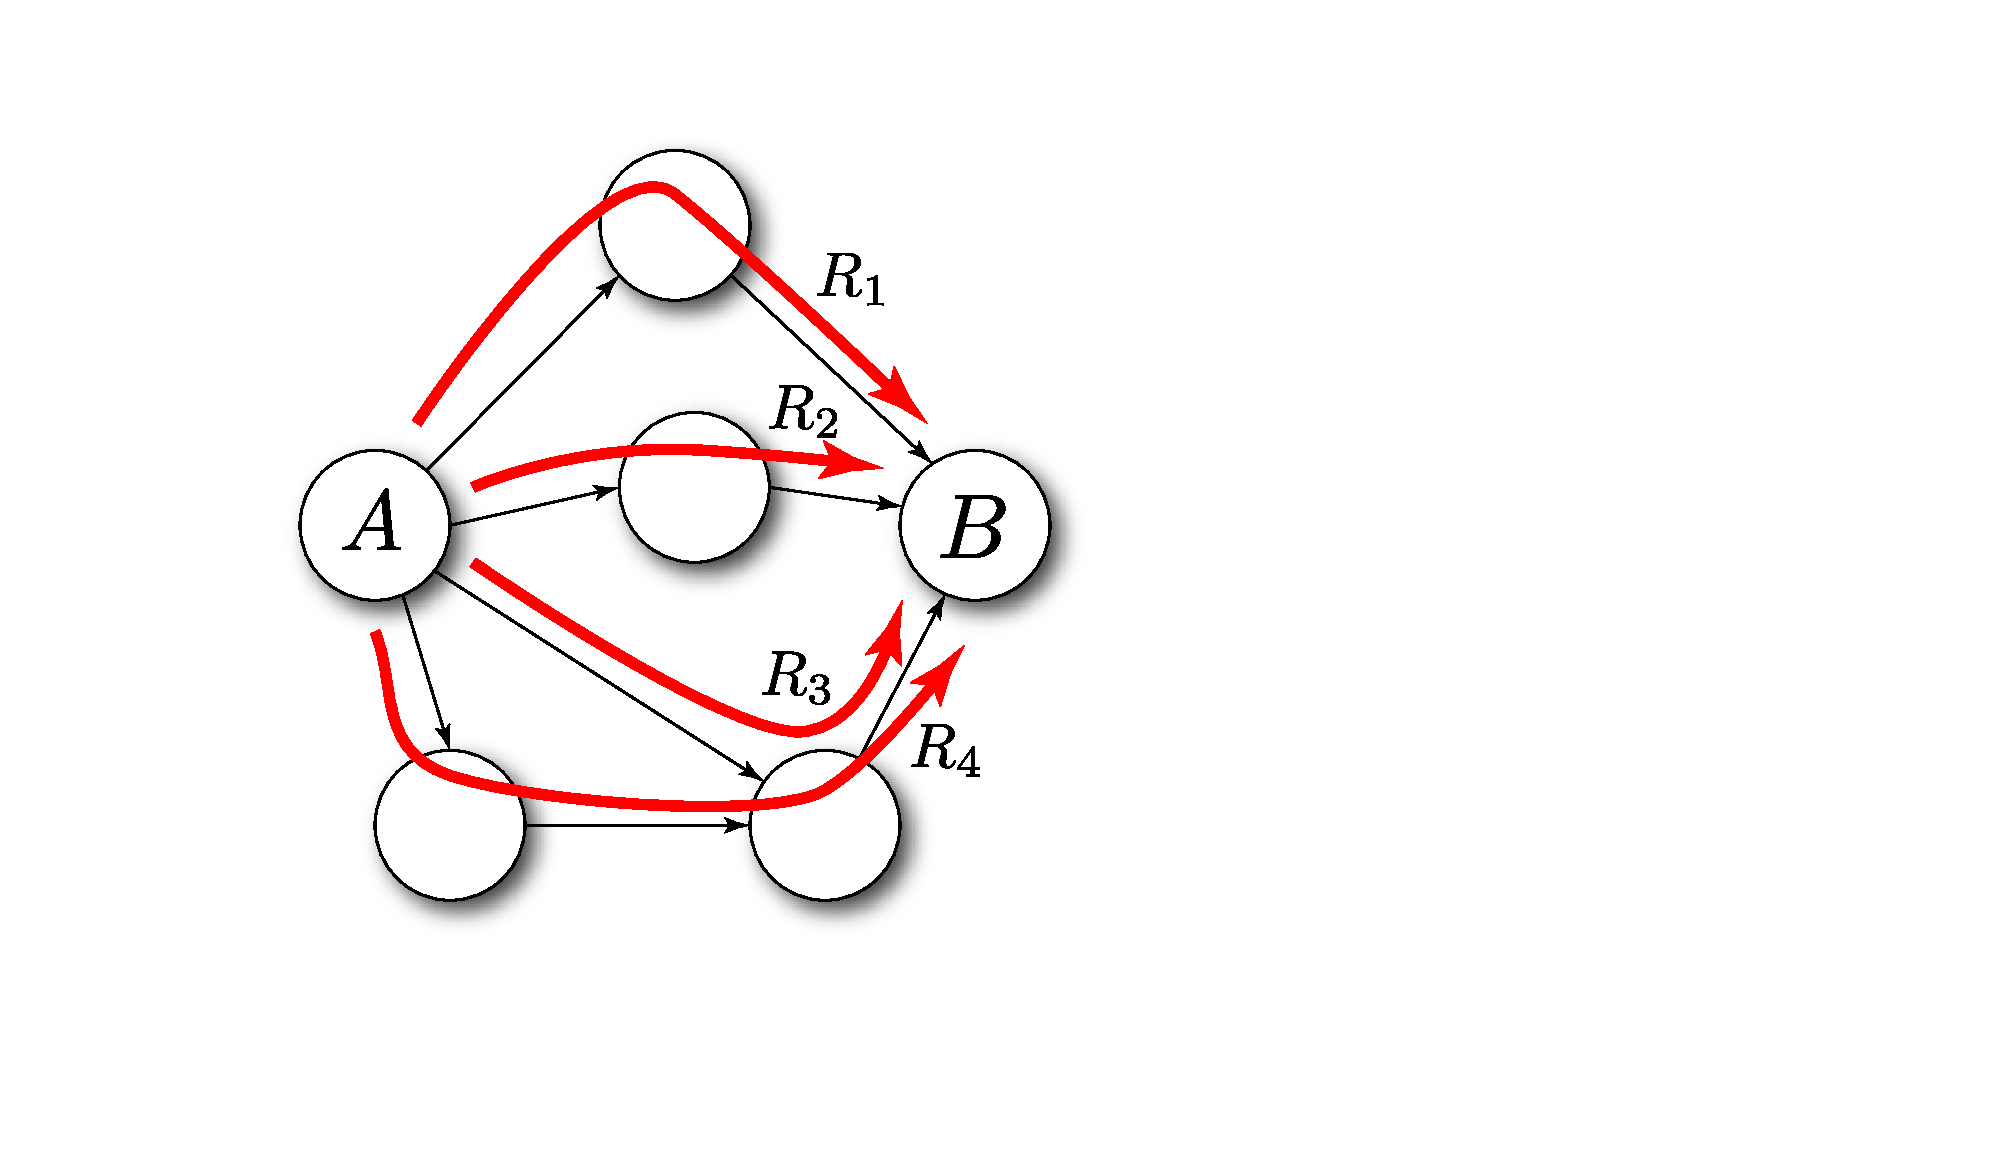
\includegraphics[width=0.65\columnwidth]{example_routes}
\caption{Example of a simple network with multiple routes \mbox{$A\to B$}. Note that $R_3$ and $R_4$ are competing with one another for use of the last link, which the routing strategy, $\mathcal{S}$, will need to resolve if multiple simultaneous transmissions are taking place.} \label{fig:example_routes}
\end{figure}

\begin{figure}[!htb]
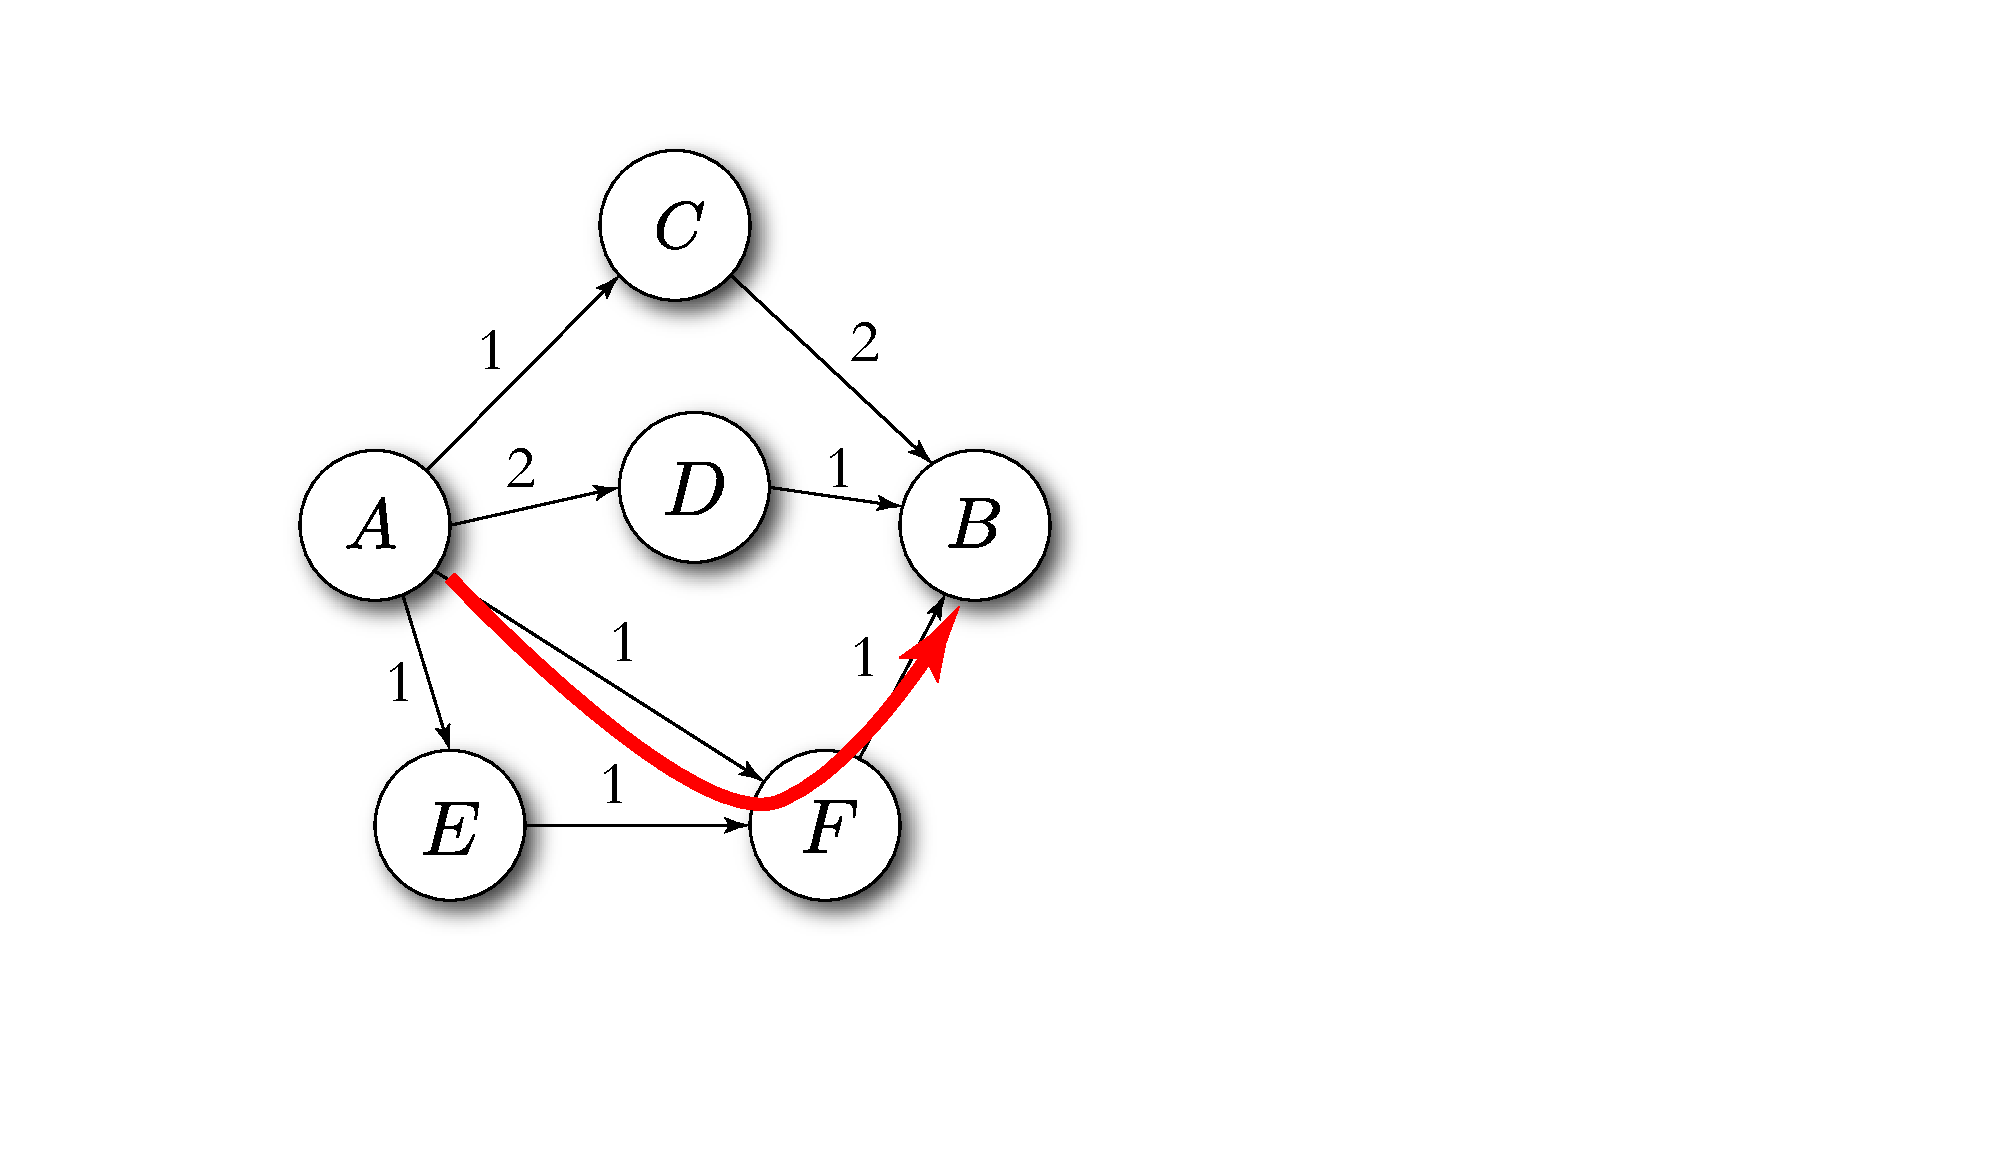
\includegraphics[width=0.6\columnwidth]{example_opt}
\caption{The same network graph from Fig.~\ref{fig:example_routes}, with links weighted by some arbitrary cost metric. Applying a shortest-path algorithm yields the optimal route between Alice and Bob to be \mbox{$A\to F\to B$}, which incurs a net cost of \mbox{$c=2$}, as opposed to all other routes, which incur a net cost of \mbox{$c=3$}.} \label{fig:simp_route_opt}
\end{figure}

In a given network, it is unlikely that only a single cost metric or attribute will be of interest when determining optimal routings. There may be a tradeoff between different measures. For example, for time-critical applications the cost of a route might be considered a combination of both dollar cost and latency -- a satellite has very low latency but is extremely expensive, while a carrier pigeon is slow but cheap (and prohibited by PETA). What is the best tradeoff between the two?

To accommodate this, we allow the \textit{net cost} of a route to be defined as an arbitrary function of other primitive cost metrics and attributes of the route,
\begin{definition}[Net routing cost]\index{Net routing cost}
The net cost of a route \mbox{$A\to B$} is given by,
\begin{align} \label{eq:net_cost_R} \index{Net cost}
c_\text{net}(R) = f_\text{cost}(\vec{c}(R),\vec{a}(R)),
\end{align}
where $c_\text{net}$ is a single numeric value representing the net cost as calculated from an arbitrary cost function, $f_\text{cost}$, of the vector of associated costs and attributes.
\end{definition}
Note that the net routing cost needn't be a metric, as the cost function could be arbitrary. The net cost can be thought of as a ranking for routes, but not necessarily as a metric that accumulates across routes, since it already captures all these accumulations.

Eq.~(\ref{eq:net_cost_R}) gives us the net cost of a given route. For multiple users we would like to simultaneously optimise the cost across all users of the network. Thus we define the routing cost for the entire network to be,
\begin{definition}[Network routing cost]
	The net routing cost of all costs, over all active routes $\vec{R}$ is,
\begin{align} \label{eq:c_total}
c_\text{total}(\vec{R}_{\vec{A}\to \vec{B}}) = \sum_{r \in {\vec R}_{\vec{A}\to \vec{B}}} c_\text{net}(r),
\end{align}
where $\vec{R}_{\vec{A}\to \vec{B}}$ is a set of active routes connecting each pair \mbox{$A_i\to B_i~\forall ~ i$}.
\end{definition}

%
% Flow Networks
%

\subsection{Flow networks} \label{sec:flow_networks} \index{Flow networks}

On a shared network with many users utilising the network simultaneously, it may be the case that the preferred goal for the network is to maximise \textit{flow} \cite{???} -- the total amount of information that can be transmitted per unit time, i.e the net utilisation of the network's resources, summed over all users. In this case we can build on the existing theory of \textit{flow networks} \cite{???}, which characterise the load of links within the network.

A flow network is easily obtained from the network graph by associating a `capacity' attribute with each link and defining the graph weighted by the capacities as the flow network, preserving the underlying structure of the network graph.

When a route within the graph is utilised, we decrement the capacities of each link in that route, generating the so-called \textit{residual network} \cite{???}, which will now take the place of the original network in subsequent calculations. This process effectively tallies the links' utilisation, and when the tally hits zero, the link can no longer be used for any new routes. This forms a basic building block for more complex flow network algorithms.

There are many variations on flow networks. The simplest case is of a single user transmitting multiple packets simultaneously to a recipient. Depending on link capacities, different packets may need to follow different routes through the network, if network performance is to be maximised. Alternately, it may not be possible to send the desired number of packets simultaneously if the network capacity saturates.

The more complex (and realistic) scenario is of multiple users each transmitting from distinct starting nodes to distinct recipient nodes across a shared network. This is known as a \textit{multi-commodity flow network} \cite{???}, and is likely to be the dominant class of networks in real-world networking applications.

%
% Routing Strategies
%

\subsection{Routing strategies} \label{sec:route_strats} \index{Routing strategies}

A \textit{strategy}, $\mathcal{S}$, is simply an algorithm that chooses a route, based on the starting and finishing nodes of a communication, and also updates the vectors of costs and attributes within the network associated with the utilisation of that route,
\begin{definition}[Routing strategies]
A routing strategy is defined by,
	\begin{align}
\mathcal{S}(i,j,\vec{c},\vec{a}) &\to \{k,{\vec{c}}~',{\vec{a}}~'\}, \nonumber \\
i,j &\in V, \nonumber\\
k &\in \{R_{v_i\to v_j}\},
\end{align}
where $\mathcal{S}$ denotes the strategy, $k$ is a route, $i$ and $j$ are the source and destination nodes of the route, and $\vec{c}$ and $\vec{a}$ are vectors of associated costs and attributes.
\end{definition}
The goal of the strategy $\mathcal{S}$ is to minimise a chosen cost measure.

No particular route through a network is going to have infinite capacity, and therefore we cannot typically always reemploy the same most cost-effective route for all data. Particularly in multi-user networks, as routes are employed for communicating quantum states, their cost metrics may change according to load, or other external influences. Alternately, some routes may come into and out of operation. For example, a satellite requiring line-of-sight communication may oscillate in and out of sight, thereby periodically enabling and disabling respective network routes. For this reason, it is important that strategies accommodate dynamic changes in the network. This is easily accounted for by letting the edge weights in our network graph be a function of time, $G_t$, which are updated via the application of a strategy, which may also be time-dependent,
\begin{definition}[Time-dependent routing strategies]
A time-dependent strategy, $\mathcal{S}_t$, updates the network graph, $G_t$, at each time-step $t$,
\begin{align} \label{eq:S_G}
G_{t+1} = \mathcal{S}_t(G_t).
\end{align}
\end{definition}
For example, the network might have bandwidth restrictions on some links, in which case if more than a certain amount of data is transmitted through a link, it is no longer available for use until previous transmissions have completed. Or, based on market dynamics, the dollar cost of utilising a link may change with its demand.

This type of cost minimisation approach to routing is analogous to \textit{distance-vector routing protocols}\index{Distance-vector routing protocols} in classical networking theory.

A detailed exposition of routing strategies is provided in Sec.~\ref{sec:strategies}.

%
% Strategy Optimisation
%

\subsection{Strategy optimisation} \label{sec:strat_opt} \index{Strategy optimisation} 

Clearly the goal when choosing routing strategies is to minimise the total cost, Eq.~(\ref{eq:net_cost_R}). That is, solving the optimisation problem,
\begin{definition}[Strategy optimisation]
The optimisation of strategies with a network comprising net costs $c_\text{total}$ is given by,
\begin{align}
c_\text{min} &= \underset{\mathcal{S}}{\text{min}}(c_\text{total}), \nonumber \\
\mathcal{S}_\text{opt} &= \underset{\mathcal{S}}{\text{argmin}} (c_\text{total}).
\end{align}
\end{definition}

Choosing optimal strategies is a challenging problem, potentially requiring complex, computationally inefficient optimisation techniques. Strategy optimisation is an example of resource allocation, whose optimal solutions are often notoriously difficult to solve exactly, residing in complexity classes like \textbf{NP}-complete\index{\textbf{NP} \& \textbf{NP}-complete} (or worse!). In general, the number of possible routes through a graph will grow exponentially with the number of vertices. Thus, explicitly enumerating each possible route is generally prohibitive for large networks, unless some known structure provides `shortcuts' to optimisation. Having said this, Dijkstra's shortest path algorithm (discussed in Sec.~\ref{sec:shortest_path}) is the perfect counterexample, demonstrating that although an exponential number of routes may exist between two points, an optimal one can be found in \textbf{P}.

%
% Ad hoc Operation vs. Central Authorities
%

\subsubsection{Ad hoc operation vs. central authorities} \index{Central authorities} \index{Ad hoc networks}

When considering strategy optimisation, the first question to ask is `Who performs the optimisation, and who has access to what information?'.

In terms of who performs the optimisation, the two main options are that either each node is responsible for optimising the routes of packets passing through it (\textsc{Individual} algorithms), or there is a reliable and trusted central authority who oversees network operation and performs all strategy decision-making (\textsc{Central} algorithms).

In the case of \textsc{Individual} algorithms, the required knowledge of the state of the network could be obtained using network exploration algorithms (Sec.~\ref{sec:path_exp}) or gateway protocols (Sec.~\ref{sec:gateway}). 

On the other hand, for \textsc{Central} algorithms, either network exploration could be employed, or alternately the network policy could require nodes to notify the central authority upon joining or leaving the network. The former introduces an overhead in classical networking resource usage, since network exploration must be performed routinely to keep the ledger of nodes up-to-date. The latter, on the other hand, avoids this, but introduces a point of failure, in that all network participants must be reliable in notifying the central authority as required by the network policy. Failure to do so could result in invalid or suboptimal strategies.

%
% Local vs. Global Optimisation
%

\subsubsection{Local vs. global optimisation} \index{Local optimisation}\index{Global optimisation}

There are two general approaches one might consider when choosing strategies -- \textit{local optimisation} (\textsc{Local}) and \textit{global optimisation} (\textsc{Global}). \textsc{Local} simply takes each state to be communicated, one-by-one, and allows it to individually choose an optimal routing strategy based on the state of the network at that moment. \textsc{Global} is far more sophisticated and simultaneously optimises the sum of the routing costs, Eq.~(\ref{eq:c_total}), of all currently in-demand routes.

To implement \textsc{Local} optimisation, either \textsc{Individual} or \textsc{Central} algorithms may be employed. On the other hand, \textsc{Global} optimisation necessarily requires a \textsc{Central} algorithm, since it requires knowledge of the entire state of the network, which is collectively optimised.

Since \textsc{Global} represents the class of all algorithms that take all network costs by all packets into consideration, it must clearly perform at least as well as \textsc{Local}, which only takes into consideration the costs of a given packet. But we expect \textsc{Global} to perform better than \textsc{Local} in general, owing to the additional information it takes into consideration. We express this as \mbox{\textsc{Local}$\subset$\textsc{Global}}. However, \textsc{Global} requires solving a complex, simultaneous optimisation problem, which is likely to be computationally hard, whereas \textsc{Local} can be efficiently solved using multiple independent applications of, for example, an efficient shortest-path algorithm (so-called \textsc{Greedy} algorithms), discussed in Sec.~\ref{sec:shortest_path}.

A further stumbling block for \textsc{Global} is that it requires some central authority, responsible for the global decision-making, to have complete, real-time knowledge of the state of the entire network. This may be plausible for small LANs, but would clearly be completely implausible for the internet as a whole. So it is to be expected that different layers and subnets in the network hierarchy will employ entirely different strategy optimisation protocols. This is certainly reminiscent of the structure of the present-day internet.

Roughly speaking, we might intuitively guess that at lower levels in the network hierarchy, responsible for smaller subnets, there will be a tendency towards the adoption of \textsc{Global} strategies, as full knowledge of the state of the subnet is readily obtained and maintained. However, as we move to the highest levels of the network hierarchy (e.g routing of data across international or intercontinental boundaries), we might expect more laissez-faire (i.e \textsc{Greedy}) strategies to be adopted, since the prospects of enforcing a central authority with full knowledge of the state of the internet, who is also trusted by all nations to fairly and impartially allocate network resources and mediate traffic, is highly questionable.

We will not aim to comprehensively characterise the computational complexity of \textsc{Global} strategies. However, in Sec.~\ref{sec:strategies} we will present some elementary analyses of several toy models for realistic strategies. Some such strategies are efficient although not optimal, but nonetheless satisfy certain criteria we might expect.

Future developments in the optimisation techniques required for \textsc{Global} strategies may improve network performance, leaving our techniques qualitatively unchanged.

When employing \textsc{Local}, on the other hand, things are often far simpler. If we are optimising over a cost metric satisfying the distance interpretation, we may simply employ a shortest-path algorithm to find optimal routes through the network.

If one were to become even more sophisticated, one might even envisage treating network resource allocation in a game theoretic context \cite{???}, which we won't even begin to delve into here.

%
% Message- vs. Packet-Level Routing
%

\subsection{Message- vs. packet-level routing}

In Eq.~(\ref{eq:S_G}) we defined the action of a strategy, $\mathcal{S}$, on a network, $G$. However, we were intentionally ambiguous in our introduction of the time-dependence, given by $t$. This is to allow us to consider changes at one of two different time-scales: the packet level, or the message level. The \textit{message} is the entire data stream transmitted from Alice to Bob, whereas the \textit{packet} is a small block of data taken from the message, where each packet may be independently routed.

When defining the action of strategies, we could do so at either of these time-scales. We could choose routes in their entirety, from start to finish, at the beginning of the message transmission, under the assumption that the costs in the network will be constant over that duration and no one will misbehave. We refer to such strategies as \textit{message-level strategies}. Alternately, and perhaps more realistically in many scenarios, the costs and attributes of a network could be highly dynamic and readily change within the transmission time-window. In that case, we will employ \textit{packet-level strategies}, which reevaluate the strategy independently for each packet and for each of their hops between nodes.

In our future discussions on routing strategies, context will make it clear when we are referring to packet- or message-level strategies.
\sketch{sketch_8}

\latinquote{Nil sine magno labore.}

%
% Network Topologies
%

\section{Network topologies} \index{Network topologies}\label{sec:network_topologies}

\dropcap{A}{s} quantum (or classical) networks inherently reside on graphs, it is important to introduce some of the key graph structures of relevance to networking and some of their properties of relevance to quantum networking protocols.

Let the graph $G$ representing the network be,
\begin{align}
G=(V,E),	
\end{align}
with vertices $V$ and edges $E$. In principle a network could be characterised by any connected graph whatsoever. However, there are certain structures and patterns that emerge very frequently and deserve special attention.

It is paramount that QTCP protocols have the capacity to deal with the diverse network topologies that are likely to present themselves in the future real-world quantum internet. Some of the graph-theoretic algorithms that we rely on in our QTCP protocol (Sec.~\ref{sec:graph_theory}) are computationally efficient for \textit{arbitrary} graph topologies, even more so for certain classes of graphs exhibiting particular structure, such as tree graphs or complete graphs. Others, however, are computationally inefficient in general, but may have efficient approximation algorithms for some or all classes of topologies.

We will now review some of the graph structures most likely to arise in quantum networks, learning from the structures that have become ubiquitous in classical networking.

%
% Point-To-Point
%

\subsection{Point-to-point} \index{Point-to-point topologies}

The most trivial network topology, which also acts as the elementary primitive from which our other topologies will be constructed is a simple dedicated point-to-point (P2P) connection between two parties, where the sender and recipient of a packet reside on neighbouring nodes.

Such P2P connections may be reserved exclusively for the two connected neighbouring nodes. In this instance, the packets' \textsc{Routing Queue}s trivially specify just the recipient. Alternately, the P2P link may be an intermediate step between more distant sender/recipient pairs.

In the case whereby the P2P connection is reserved exclusively for a particular sender/recipient pair, the link has the property that there is no competition between multiple users sharing the channel, and the QTCP stack needn't concern itself with dynamic routing strategies\footnote{Assuming the P2P channel has sufficient capacity to meet demand and exhibits better cost metrics than other potential redundant, indirect routes.}. This significantly simplifies network scheduling algorithms (Sec.~\ref{sec:strategies}), and a \textsc{First-Come First-Served} (i.e chronologically ordered FIFO queue) strategy may be employed. Furthermore, packet collisions cannot occur, thereby improving network efficiency.

In the case whereby the P2P connection is not reserved for exclusive use between a single sender/recipient pair, but shared between different competing routes in the network, the importance of network routing strategies manifests itself. Now competition for access to the channel will reduce network efficiency, scaling inversely against the number of network participants, and the priorities and costs of packets must be tallied for the purpose of implementing routing strategies.

%
% Complete
%

\subsection{Complete} \index{Complete topologies}

The complete graph, denoted $K_{|V|}$, is a $|V|$-vertex graph where every vertex has an undirected link to every other. From a networking point of view, this can be regarded as the extremity of exclusive-use P2P networking, whereby every node has a direct link with every other. Thus, any sender can directly communicate with any receiver, via a dedicated direct channel, with no need to utilise any indirect routes. This topology has the favourable property that although any node can communicate with any other, by exclusively utilising direct P2P links we achieve several benefits:
\begin{itemize}
\item Packet collisions can be mitigated entirely, thereby maximising network efficiency.
\item Competition for the use of links can be eliminated, minimising congestion and the need for buffering (i.e quantum memory).
\item Network costs can typically be minimised, as every route only traverses a single link, and there will be no accumulation of costs.
\item The network has maximal route redundancy, making it the most tolerant against link failures\footnote{To disconnect a given node $v$ from the network, all $|v|$ links emanating from it must be broken, otherwise redundant routes to the remainder of the network will exist.}.
\item A trivial \textsc{First-Come First-Served} routing strategy can be employed, eliminating the need for any dynamic or computationally complex strategies.
\item If the network allows indirect routes to be established, the maximal redundancy of the topology also maximises the ability for routing strategies to engage in load-balancing across routes.
\item In the special case of a symmetric complete graph, whereby all edge weights are approximately equal, the shortest path between any two nodes is trivially the P2P link between them, and no complex scheduling algorithms are required.
\end{itemize}
However, these highly desirable benefits come at the expense of requiring the most elaborate and expensive network, with maximal interconnectedness.

This type of topology could arise in, for example, international-scale networks, where links of very high bandwidth (and value) between nations or continents need to be maximally utilised, which would be undermined by sparse, shared network topologies. Additionally, in this instance route redundancy will be highly valued, as the isolation of one continent from another would be catastrophic to the functioning of the global network.

Fig.~\ref{fig:complete_graph} illustrates the $K_{15}$ graph. The number of edges scales as,
\begin{align}
	|E|=O(n^2).
\end{align}
Clearly route-finding is trivial, since there is always a direct P2P link from sender to receiver, with no possibility of collisions with other packets, requiring $O(1)$ search time (assuming all users are communicating only via their direct links with one another, which may not strictly be the case when costs are factored into strategies).

\begin{figure}[!htbp]
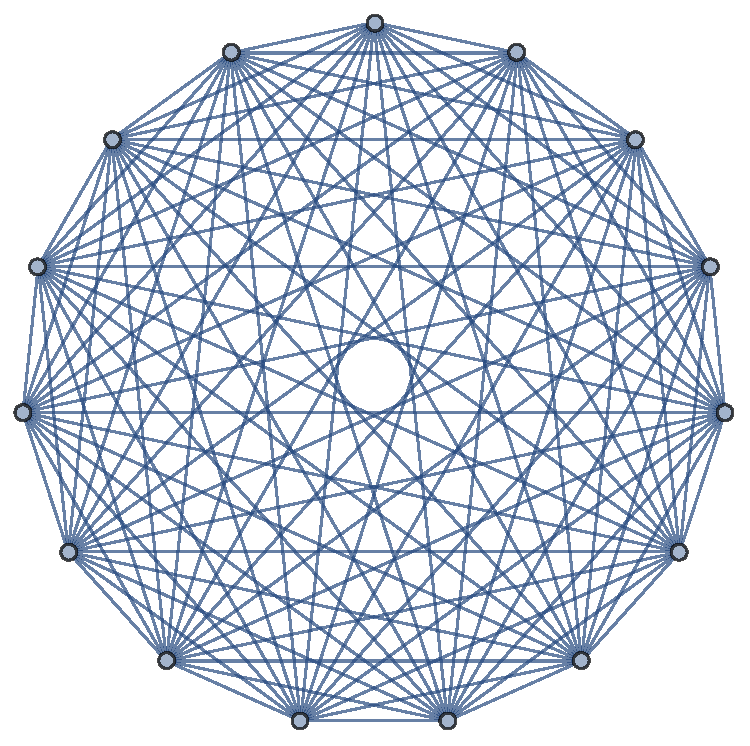
\includegraphics[clip=true, width=0.35\textwidth]{K_15}
\captionspacefig \caption{The 15-vertex complete graph, $K_{15}$. Every vertex has an edge to every other, with a total of 105 edges.} \label{fig:complete_graph}
\end{figure}

%
% Lattice
%

\subsection{Lattice} \index{Lattice topologies}

A lattice graph is simply an \mbox{$n\times m$} lattice of vertices (of any geometry, e.g squares), connecting each vertex to its immediate geometric neighbours. The number of edges scales obviously as,
\begin{align}
	|E|=O(mn).
\end{align}
This type of graph is useful when link costs are measured in terms of Euclidean distances, and nodes have nearest neighbour links, as per Fig.~\ref{fig:lattice}.

\begin{figure}[!htbp]
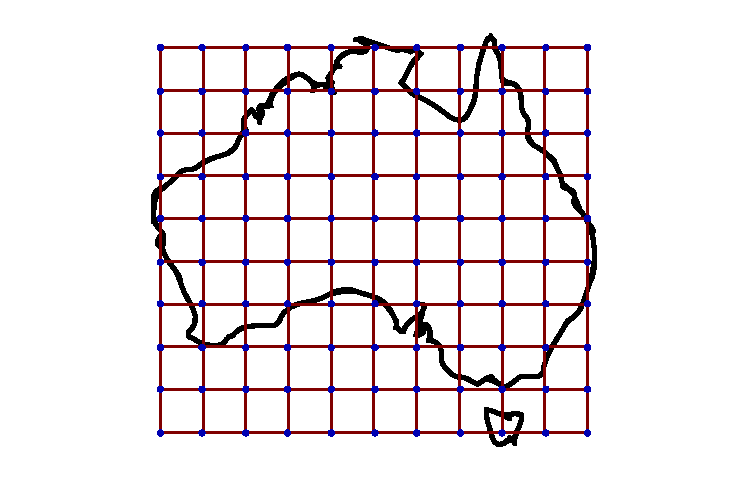
\includegraphics[clip=true, width=0.35\textwidth]{lattice}
\captionspacefig \caption{A \mbox{$10\times 11$} square lattice graph, and how it might represent a network topology with geographically associated costs. Notice that Hobart has no internet connection (why even include Tasmania at all?).} \label{fig:lattice}
\end{figure}

A slightly distorted lattice graph, in which vertices have been dragged around geometrically to match, for example, cities within a country, closely resembles the topology of the network. Similarly, if the nodes represent houses in the street layout of a highly regular city like Manhattan, a lattice may be a good approximation.

In the case of a balanced lattice, in which all edges are of equal weight, the cost of a route is the sum of the number of steps in the vertical and horizontal directions, also known as the Manhattan or $L_1$ distance,
\begin{align}
L_1 = |x_\mathrm{start} - x_\mathrm{finish}| + |y_\mathrm{start} - y_\mathrm{finish}|.
\end{align}
In this case, route finding is simplified, since \textit{all} routes, which strictly traverse in one direction vertically and one direction horizontally, are optimal and of equal distance. Thus, the diameter (maximum number of hops between any two points) on the network is,
\begin{align}
	d=O(m+n).
\end{align}

%
% Tree
%

\subsection{Tree} \label{sec:tree_graph} \index{Tree topologies}

A tree is a graph containing no cycles, only \textit{branches}\index{Branches}. There are many uses for tree graphs, but one property is of particular convenience in many applications: because the graph is acyclic, there is always exactly one path from any vertex to any other. This mitigates the need for shortest-path algorithms designed for general graphs, and simplifies route-finding algorithms (to be discussed in Sec.~\ref{sec:path_exp}). However, this brings with it the drawback that the topology is most vulnerable to link failures, since the removal of any link from the tree will separate it into a multipartite graph\index{Multipartite graphs}, making communication between the disjoint subgraphs (which are also trees) impossible, as there are no redundant routes. In a sense, tree graphs can be considered the polar opposites of complete graphs.

Trees are specified entirely by \textit{branching parameters} ($b_i$) -- the number of child nodes emanating from a given node, $i$. In general, branching parameters may be distinct for each node, although often trees with symmetries in their branching structures are considered, such as the balanced trees discussed in Sec.~\ref{sec:bal_tree}. A node terminates a branch if its branching parameter is zero (i.e it has no children).

The \textit{depth} ($d$) of a tree is the maximum number of steps from the root node to a terminating node with no children. The depth scales between \mbox{$d=O(|V|)$}, for the trivial linear tree (\mbox{$b_i=1$}), and \mbox{$d=O(\log |V|)$} for non-trivial branching parameters (\mbox{$b_i\neq 1$}).

The worst-case number of edges that must be traversed to reach any vertex from any other is,
\begin{align}
	O(\log|V|),
\end{align}
known as the \textit{diameter} of the graph\index{Diameter}, which implies that accumulated cost metrics scale similarly. Trees are the most frugal graphs in their number of edges, which are fixed at,
\begin{align}
	|E|=|V|-1,
\end{align}
irrespective of the branching parameters, since because the graph is strictly acyclic, every addition of an edge requires the addition of exactly a single vertex. This makes tree graphs the cheapest to construct in terms of physical resource usage.

%
% Balanced Tree
%

\subsubsection{Balanced tree} \label{sec:bal_tree} \index{Balanced tree topologies}

A balanced tree is a tree with a regular, self-similar structure, in which every node at a given depth is the parent of the same number of sub-nodes, all separated by the same edge weights. That is, the network has a hierarchical structure, subdividing into identically structured subnetworks. Such a network is characterised by just two parameters -- the branching parameter, $b$, and the depth, $d$. Some examples of balanced trees with different $b$ and $d$ are shown in Fig.~\ref{fig:tree_example}.

\if 2\pubmode
	\begin{figure}[!htbp]
	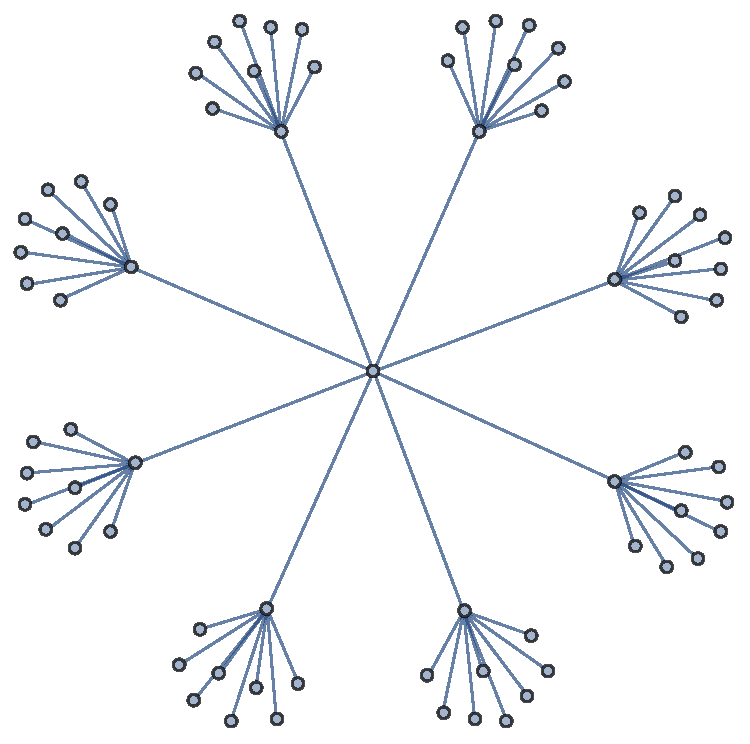
\includegraphics[clip=true, width=0.325\textwidth]{tree_3_8}\\
	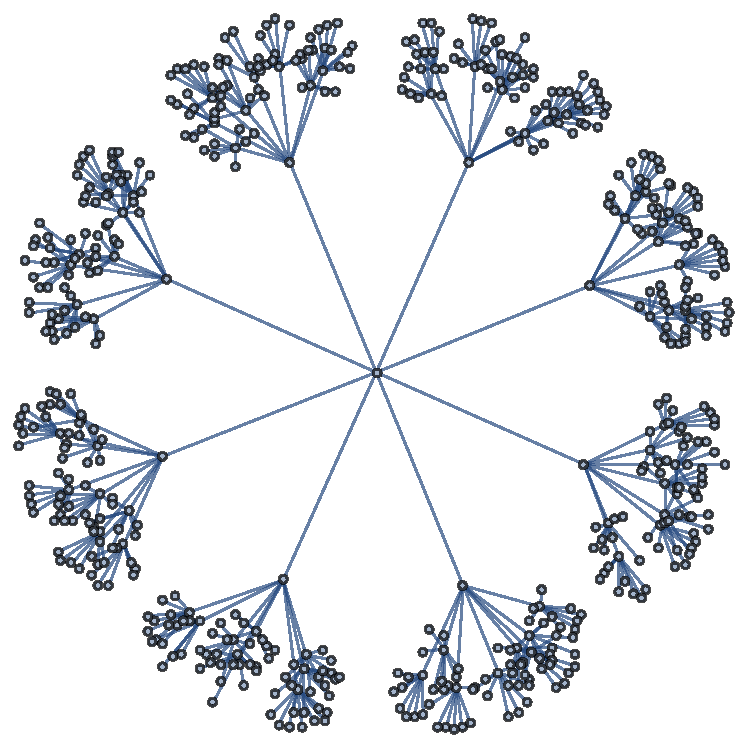
\includegraphics[clip=true, width=0.325\textwidth]{tree_4_8}\\
	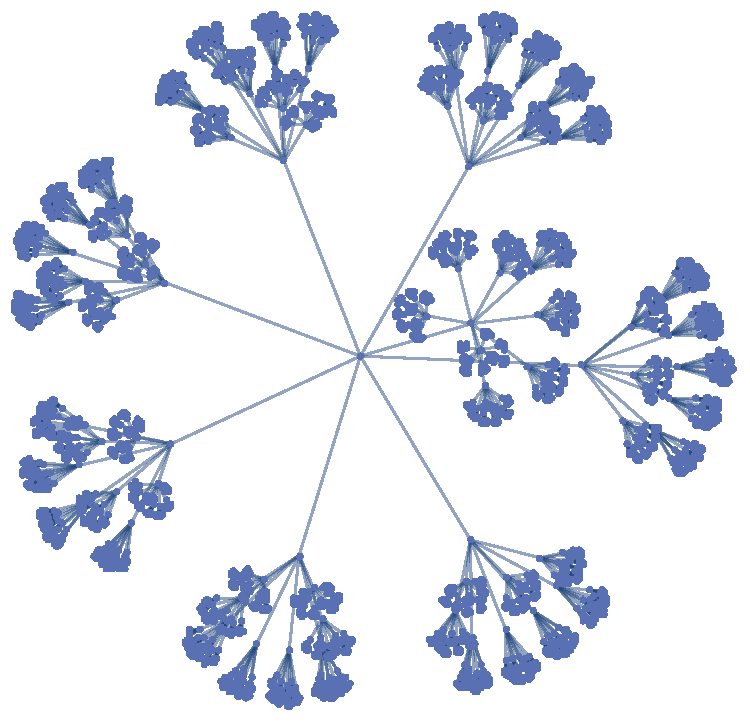
\includegraphics[clip=true, width=0.325\textwidth]{tree_5_8}
	\captionspacefig \caption{Balanced tree graphs with branching factor \mbox{$b=8$}, and depths \mbox{$d=3,4,5$}. Despite having no redundant paths, the hierarchical structure of balanced trees somewhat resembles that of real-world networks, which are typically decomposed into a pyramid scheme of progressively smaller subnetworks.} \label{fig:tree_example}
	\end{figure}
\else
	\begin{figure*}[!htbp]
	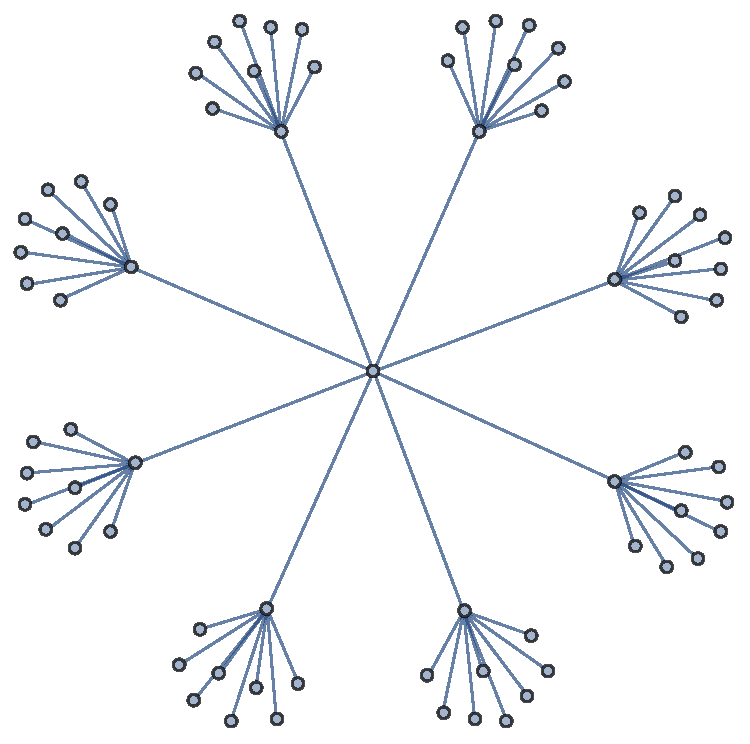
\includegraphics[clip=true, width=0.325\textwidth]{tree_3_8}
	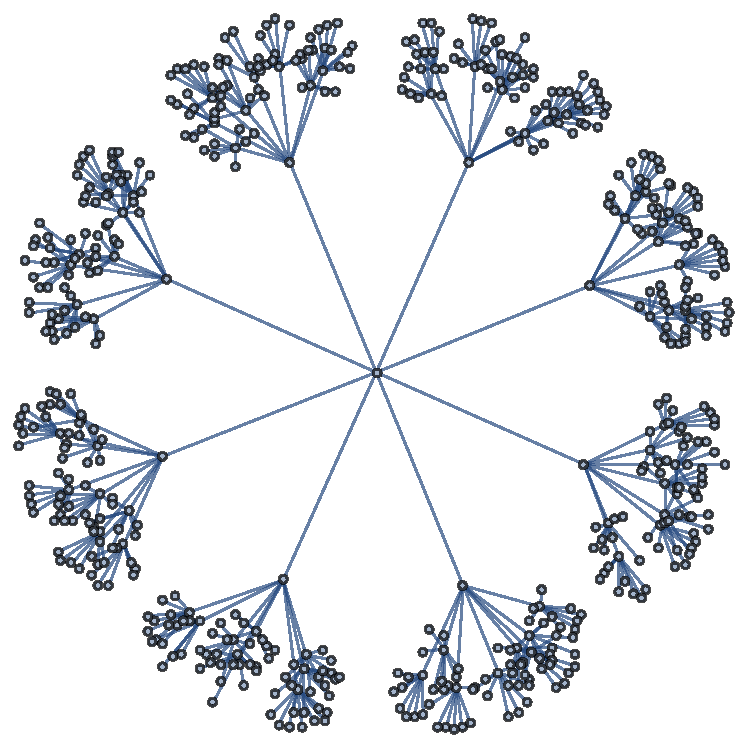
\includegraphics[clip=true, width=0.325\textwidth]{tree_4_8}
	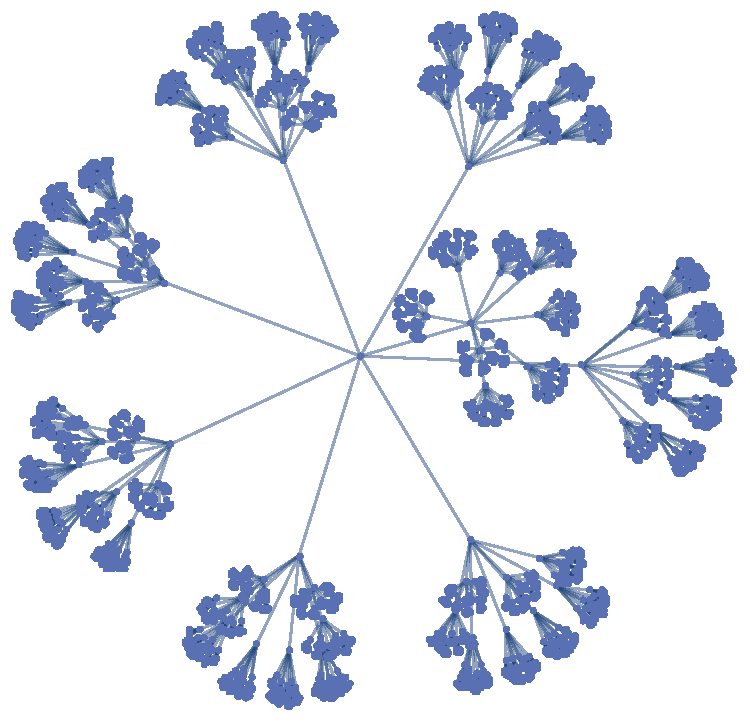
\includegraphics[clip=true, width=0.325\textwidth]{tree_5_8}
	\captionspacefig \caption{Balanced tree graphs with branching factor \mbox{$b=8$}, and depths \mbox{$d=3,4,5$}. Despite having no redundant paths, the hierarchical structure of balanced trees somewhat resembles that of real-world networks, which are typically decomposed into a pyramid scheme of progressively smaller subnetworks.} \label{fig:tree_example}
	\end{figure*}
\fi

This type of structure is (approximately) natural in many realistic scenarios. Consider for example a network containing a hierarchy of clusters of nodes representing a LAN, followed by a neighbouring internet router, followed by a city-wide router, followed by a country-wide router. In such a case, this type of general structure is typical (although more realistically one might expect the branching parameter to vary with depth).

A special case is when \mbox{$d=1$}, which we refer to as a \textit{star} graph. This might arise naturally when a series of subnets are connected together via a central router (e.g Fig.~\ref{fig:net_hierarchy}), with no further hierarchy in the network.

%
% Random Tree
%

\subsubsection{Random tree} \index{Random tree topologies}

While balanced trees accurately capture the hierarchical nature of realistic networks, they are somewhat contrived in their perfect symmetry. The subnetworks in a given network are not likely to actually all be identical. Random trees are perhaps more realistic, in that their tree structure captures the hierarchical nature of real-world networks, and also their highly ad hoc nature.

To construct a random tree we simply randomly choose a branching parameter, according to some arbitrary distribution, for every node. When a node has \mbox{$b_i=0$}, it terminates the lineage. Some examples of random trees are shown in Fig.~\ref{fig:random_tree}.

\if 2\pubmode
	\begin{figure}[!htbp]
	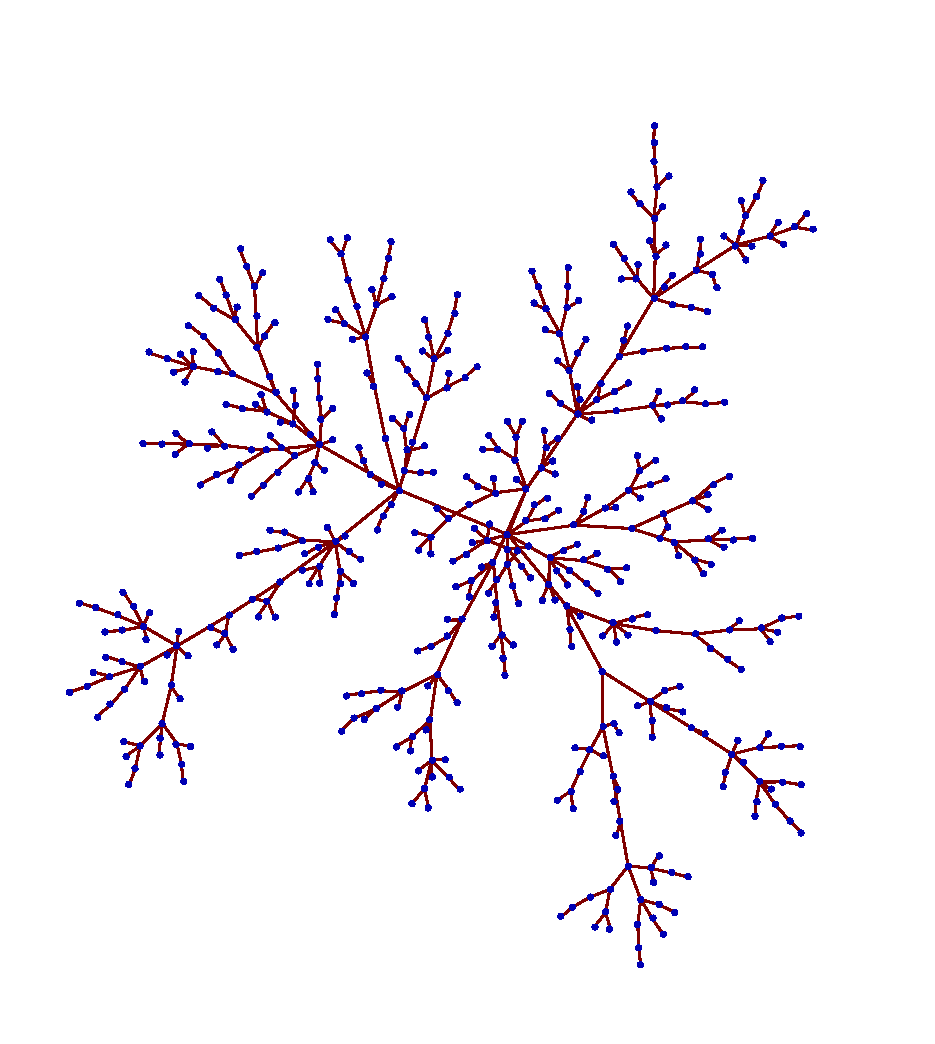
\includegraphics[clip=true, width=0.475\textwidth]{random_tree_1}\\
	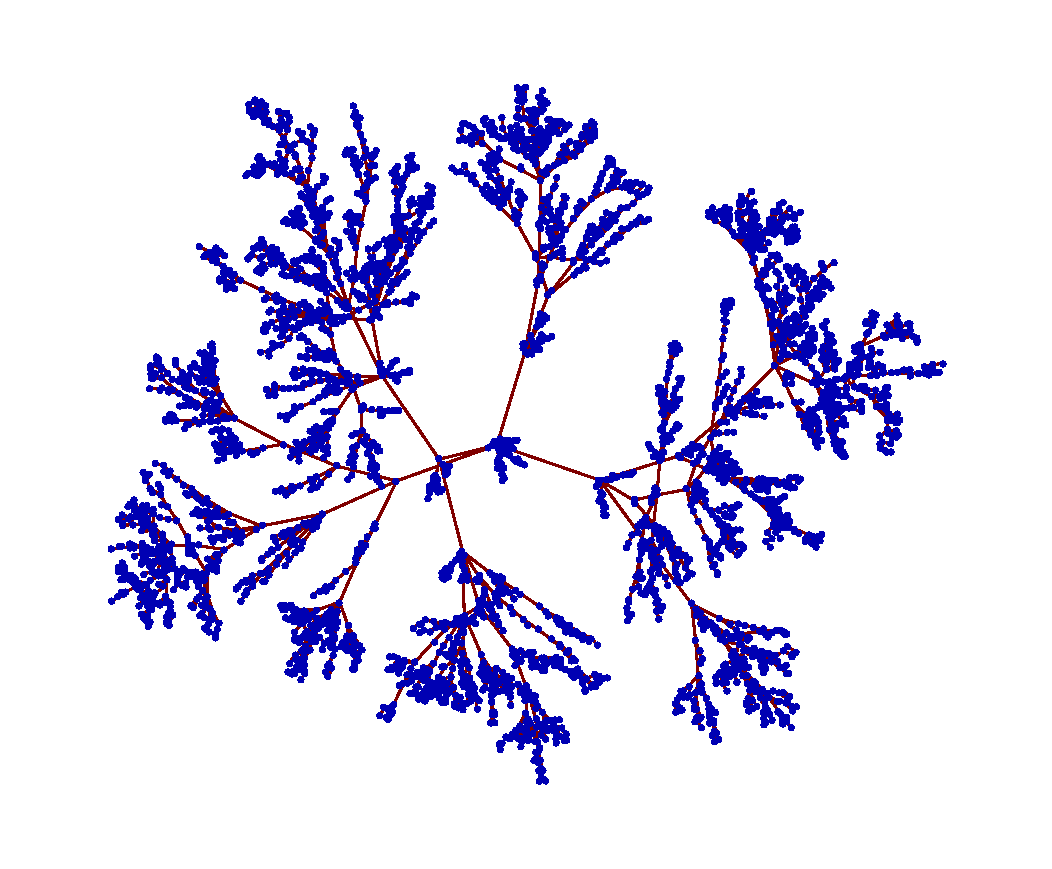
\includegraphics[clip=true, width=0.475\textwidth]{random_tree_2}
	\captionspacefig \caption{Random trees with different randomised branching parameters (higher $b$ at the bottom). When a node has zero branches, it terminates the branch. This type of graph topology qualitatively captures the hierarchical, yet ad hoc qualities of many real-world networks, and may act as a useful test model for simulations.} \label{fig:random_tree}
	\end{figure}
\else
	\begin{figure*}[!htbp]
	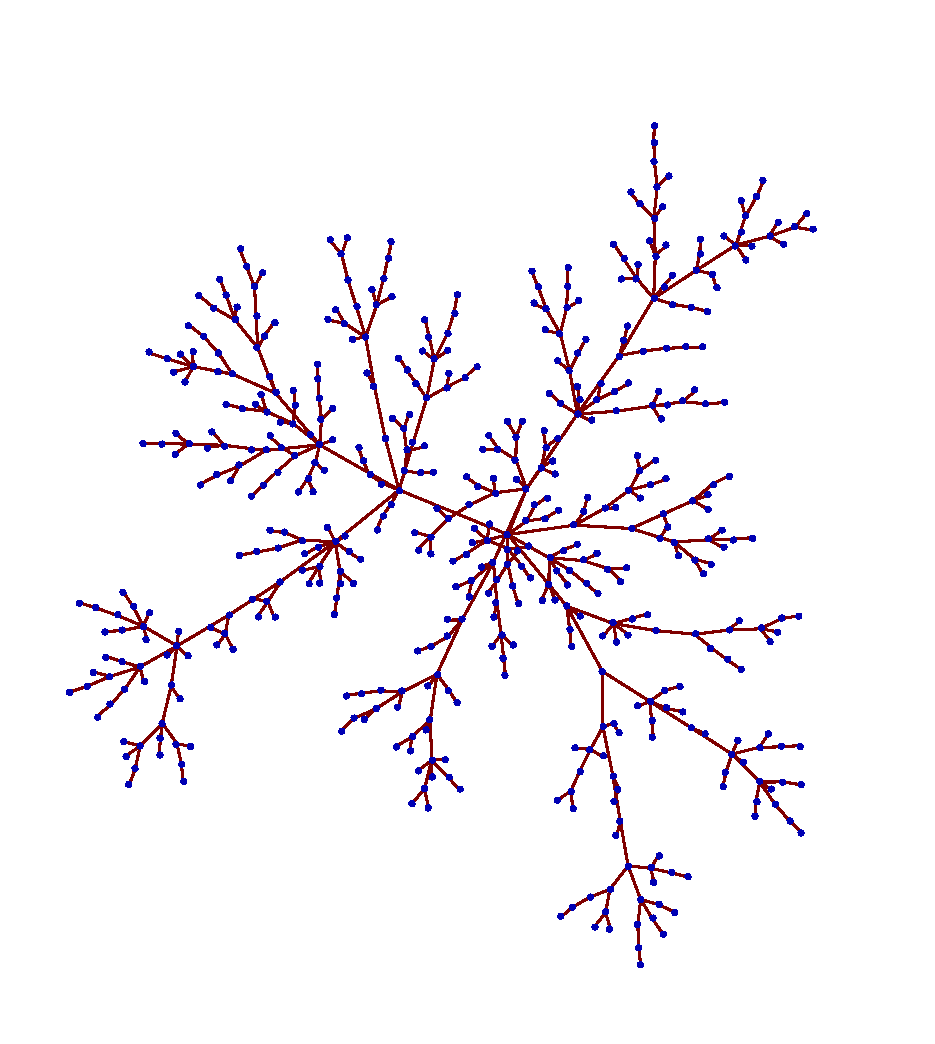
\includegraphics[clip=true, width=0.475\textwidth]{random_tree_1}
	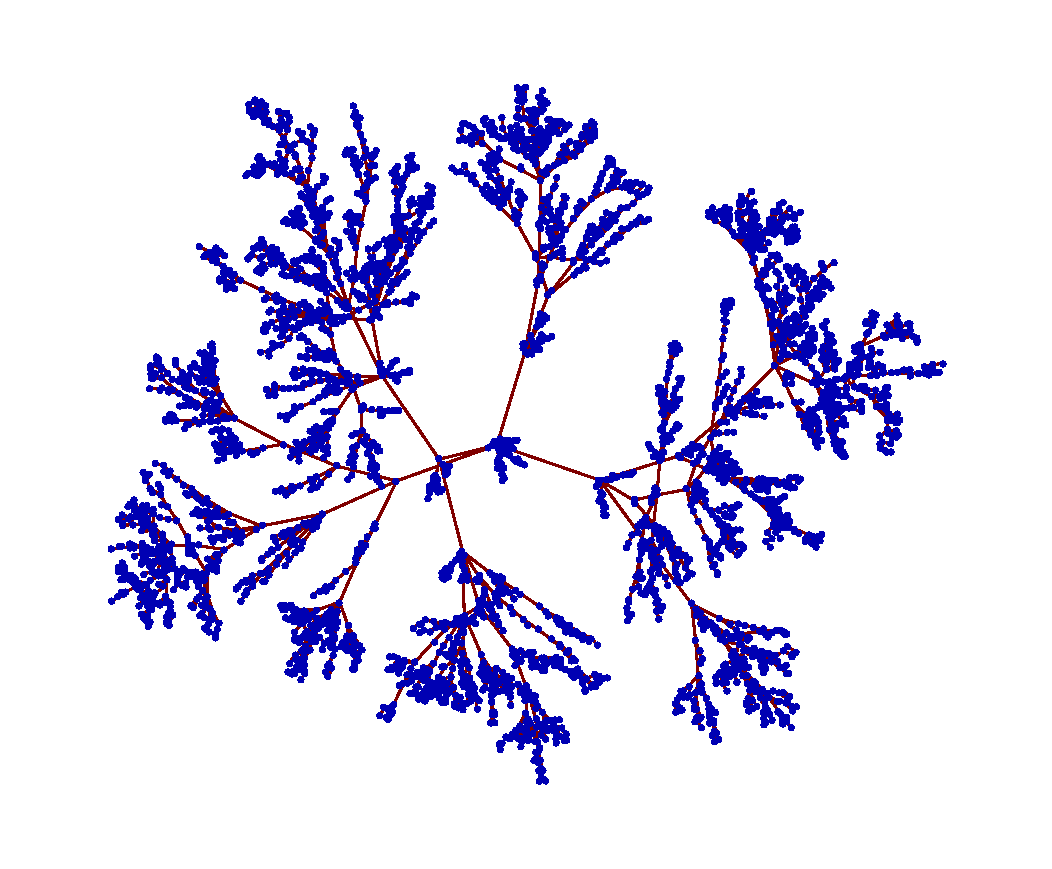
\includegraphics[clip=true, width=0.475\textwidth]{random_tree_2}
	\captionspacefig \caption{Random trees with different randomised branching parameters (higher $b$ on the right). When a node has zero branches, it terminates the branch. This type of graph topology qualitatively captures the hierarchical, yet ad hoc qualities of many real-world networks, and may act as a useful test model for simulations.} \label{fig:random_tree}
	\end{figure*}
\fi

%
% Minimum Spanning Tree
%

\subsubsection{Minimum spanning tree} \label{sec:graph_MST} \index{Minimum spanning tree}

A \textit{spanning tree}\index{Spanning tree} $S$, of a graph $G$, is a tree subgraph \mbox{$S\subset G$}, containing every vertex of $G$. The \textit{weight} of a spanning tree is the sum of all its constituent edge weights. Thus, the \textit{minimum spanning tree} (MST) is a spanning tree that minimises net weight. An example is shown in Fig.~\ref{fig:mst}. See Sec.~\ref{sec:min_tree} for a discussion on MST algorithms.

\begin{figure}[!htbp]
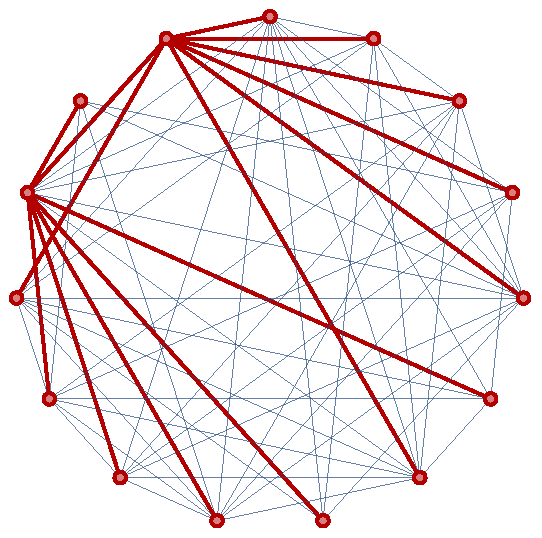
\includegraphics[clip=true, width=0.4\textwidth]{MST}
\captionspacefig \caption{A random graph (blue) with an MST highlighted (red).} \label{fig:mst}
\end{figure}

The calculation of MSTs is most likely to come into consideration when actually performing the initial construction of networks, where we wish to connect all nodes in the network, but using the most frugal possible physical resources. MSTs serve this purpose, and since they are trees, inherit all the same properties of tree networks.

%
% Percolation
%

\subsection{Percolation}\index{Percolation topologies}\label{sec:perc_topol}

A variation on any graph is to instead have a randomised implementation of it, whereby each of the possible edges or vertices occur with some probability, $p_\mathrm{edge}$ or $p_\mathrm{vertex}$, otherwise deleted. These are referred to as \textit{edge percolation} and \textit{site percolation} graphs respectively.

For any given graph, its associated percolation graph has average vertex and edge counts,
\begin{align}
|E|_\mathrm{av} &= p_\mathrm{edge}\cdot |E|,\nonumber\\
|V|_\mathrm{av} &= p_\mathrm{vertex}\cdot |V|.
\end{align}

Adjusting $p_\mathrm{edge/vertex}$ allows us to tune between the desired graph $G$ (when $p_\mathrm{edge/vertex}=1$) and the completely disconnected graph (when $p_\mathrm{edge/vertex}=0$).

This model is very useful in real-world applications, allowing unreliable channels/nodes to be incorporated into our network model. The analysis of such percolation networks is invaluable for understanding the robustness of such networks to channel and node failures.

Note that percolation graphs might be disjoint with sufficient defects, in which case the respective network becomes unreliable. Specifically, with sufficiently low $p_\mathrm{edge/vertex}$, `islands' may form in the network topology -- small segregated networks, which are unable to interface with the remainder of the network.

For asymptotically large percolation graphs, \textit{percolation theory}\index{Percolation theory} \cite{???} provides thresholds for $p_\mathrm{edge/vertex}$ such that routes across the network exist in asymptotic limits \cite{???}.

Fig.~\ref{fig:perc_graph} illustrates several square lattice graphs with different percolation probabilities, and how the larger network segregates into smaller disconnected islands as failure rates increase.

\if 2\pubmode
	\begin{figure}[!htbp]
	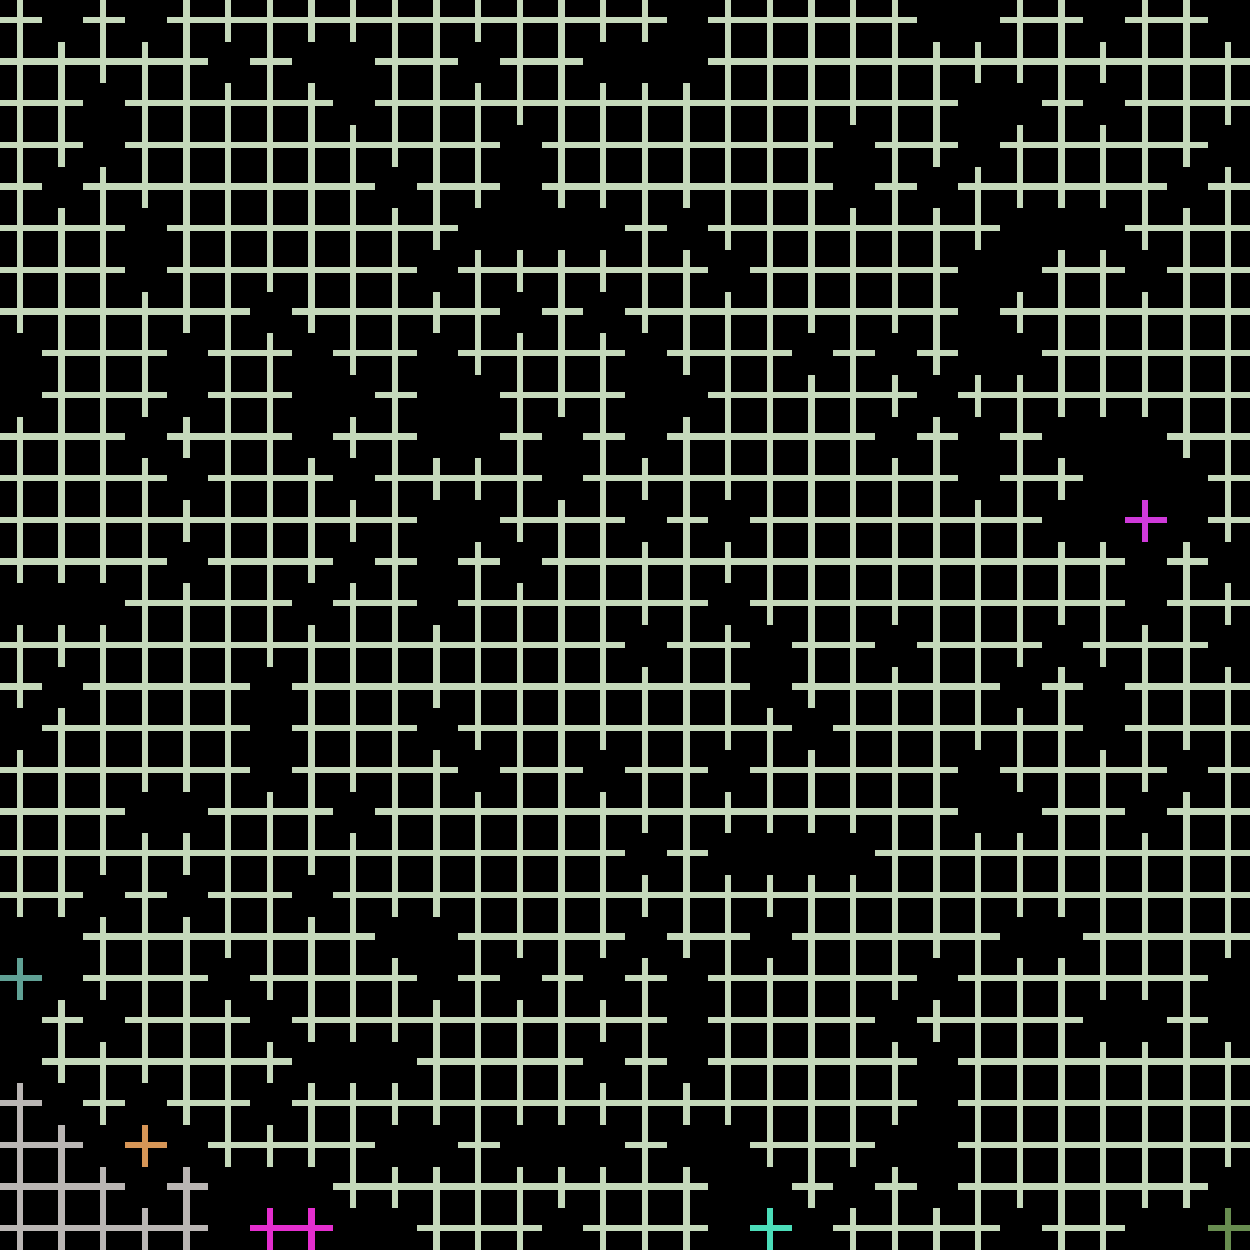
\includegraphics[clip=true, width=0.35\textwidth]{percolation_1}\\
	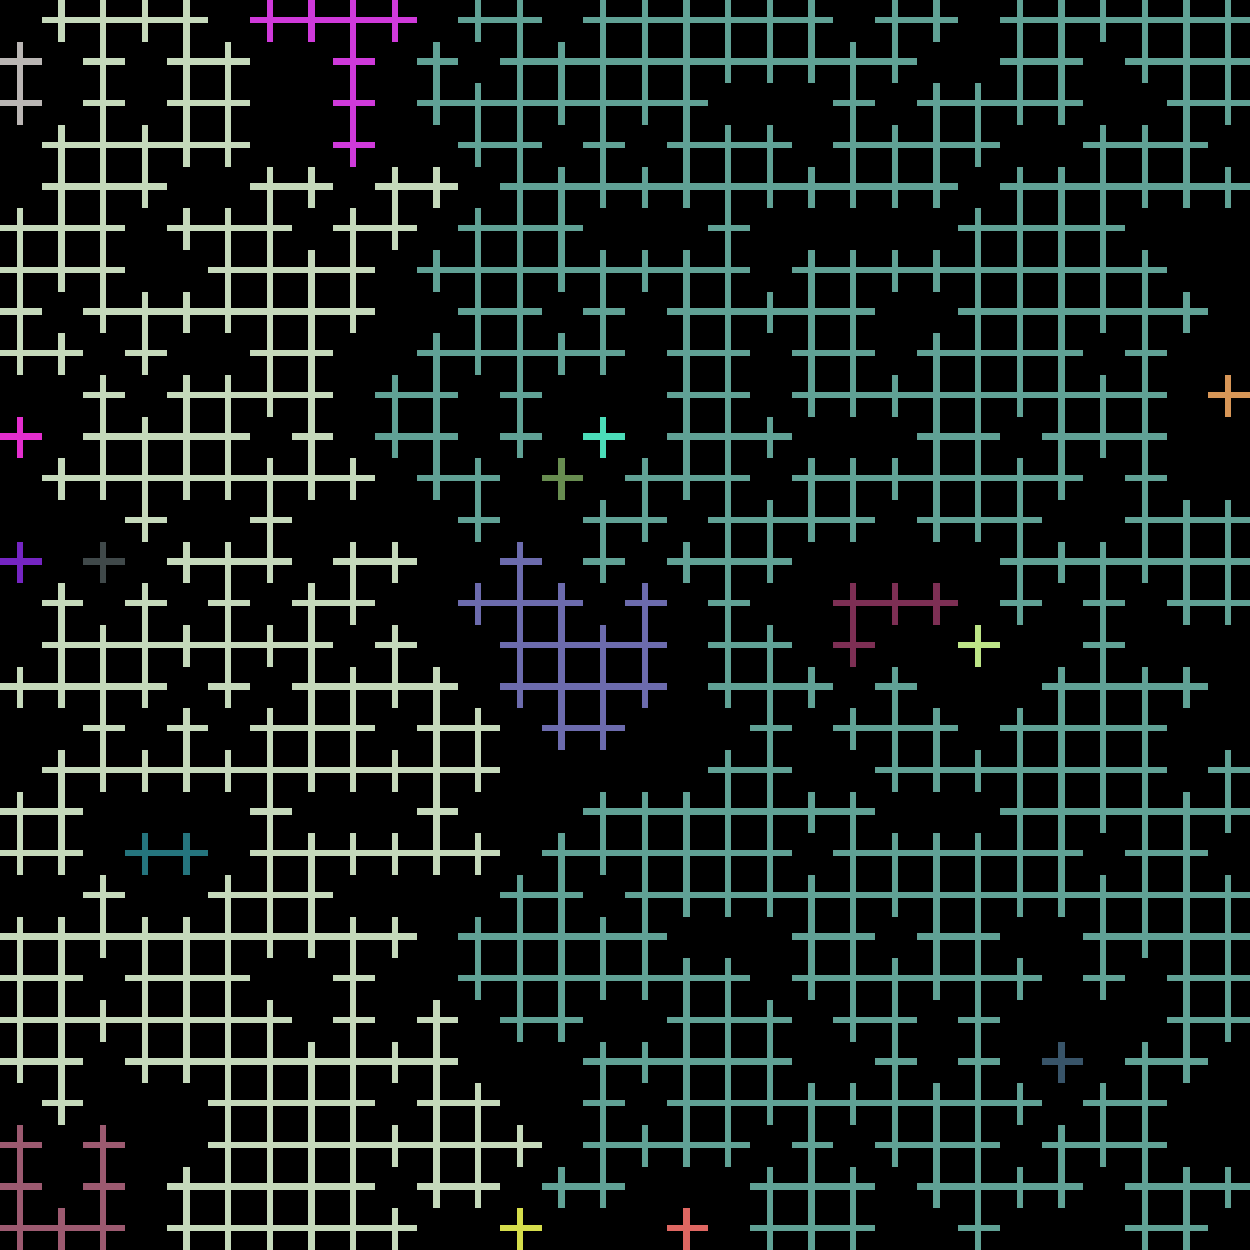
\includegraphics[clip=true, width=0.35\textwidth]{percolation_2}\\
	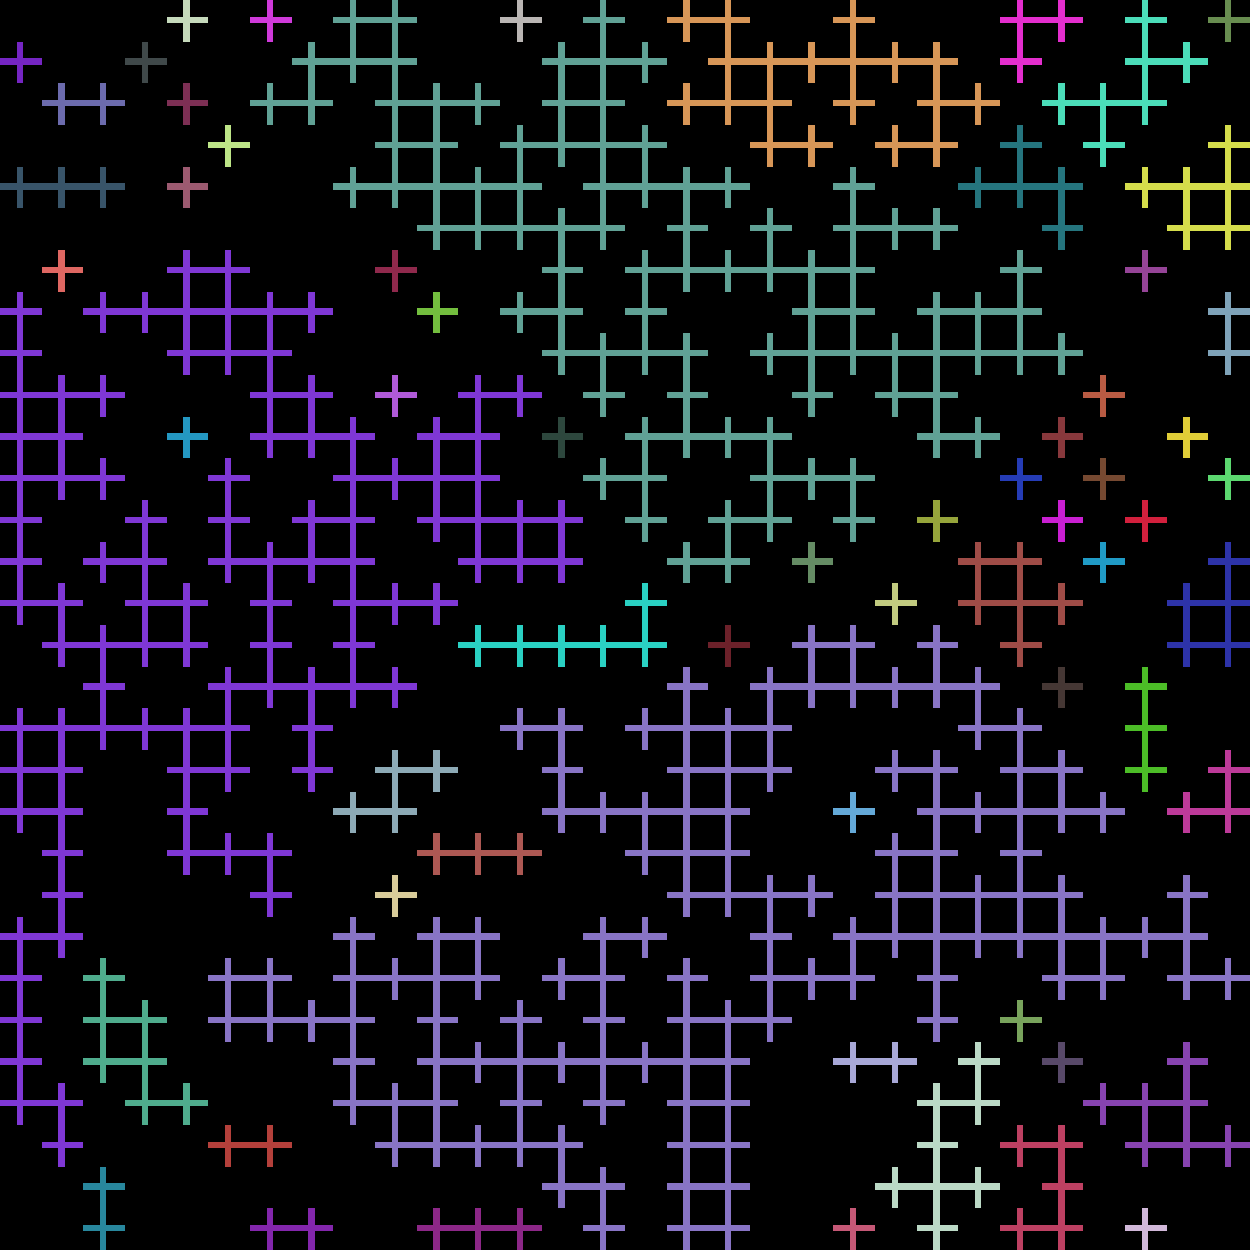
\includegraphics[clip=true, width=0.35\textwidth]{percolation_3}
	\captionspacefig \caption{A square lattice graph subject to different percolation rates (node defects). As the failure rate increases (top to bottom), the larger network segregates into a multipartite graph of smaller disjoint islands (denoted by colour).} \label{fig:perc_graph}\index{Percolation topologies}
	\end{figure}
\else
	\begin{figure*}[!htbp]
	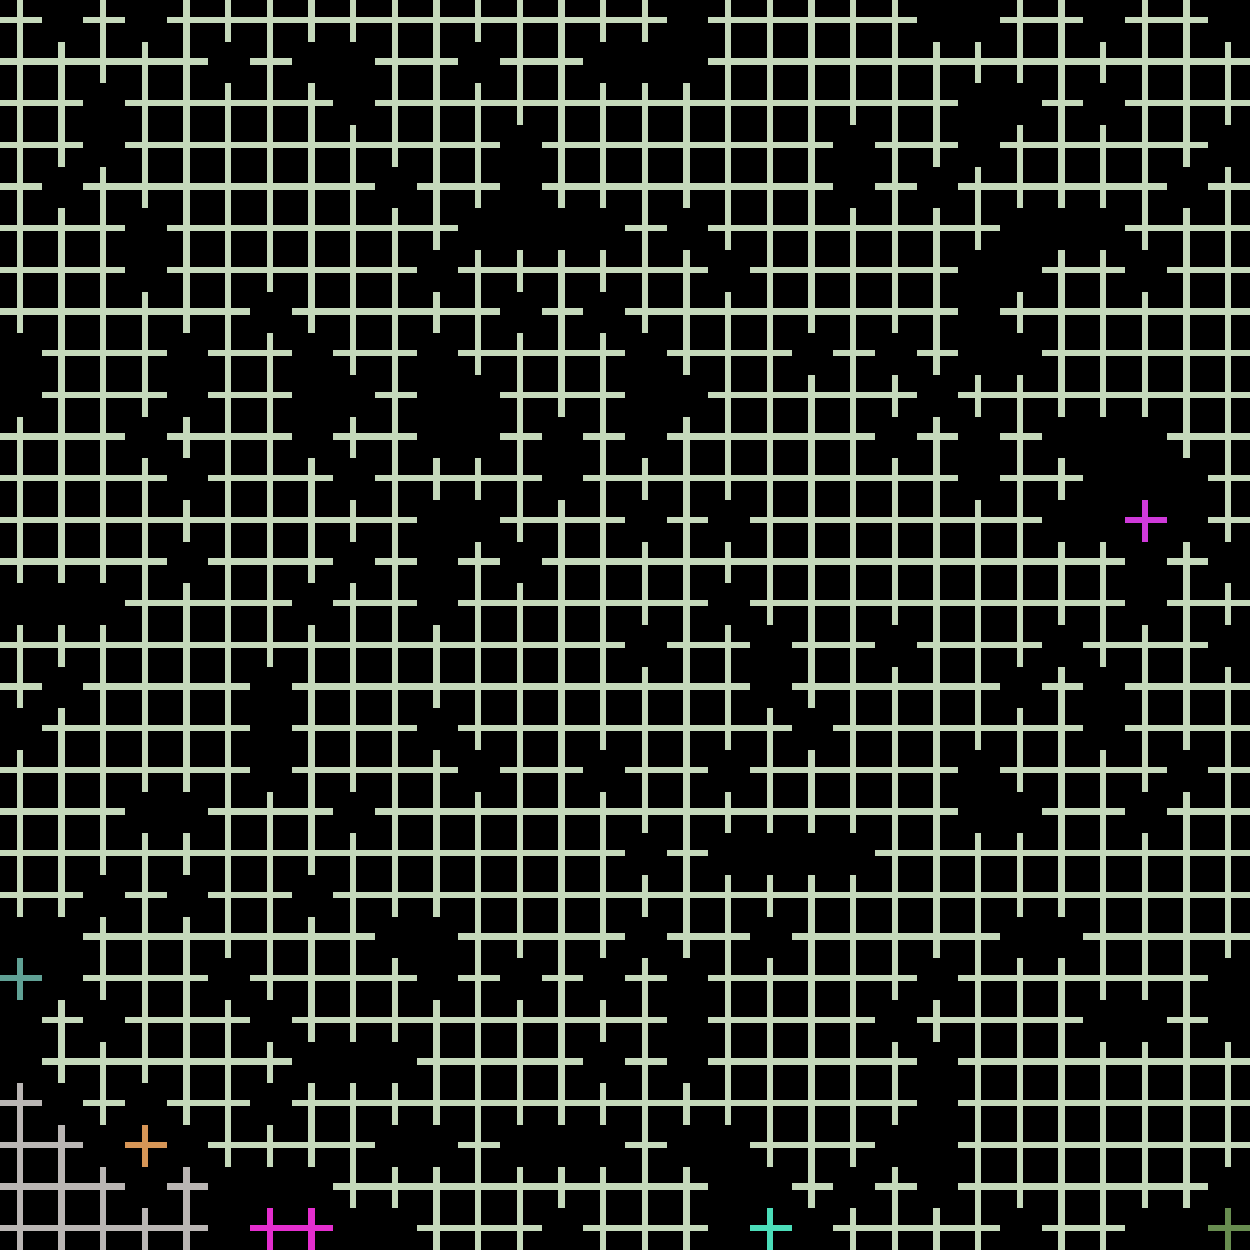
\includegraphics[clip=true, width=0.325\textwidth]{percolation_1}
	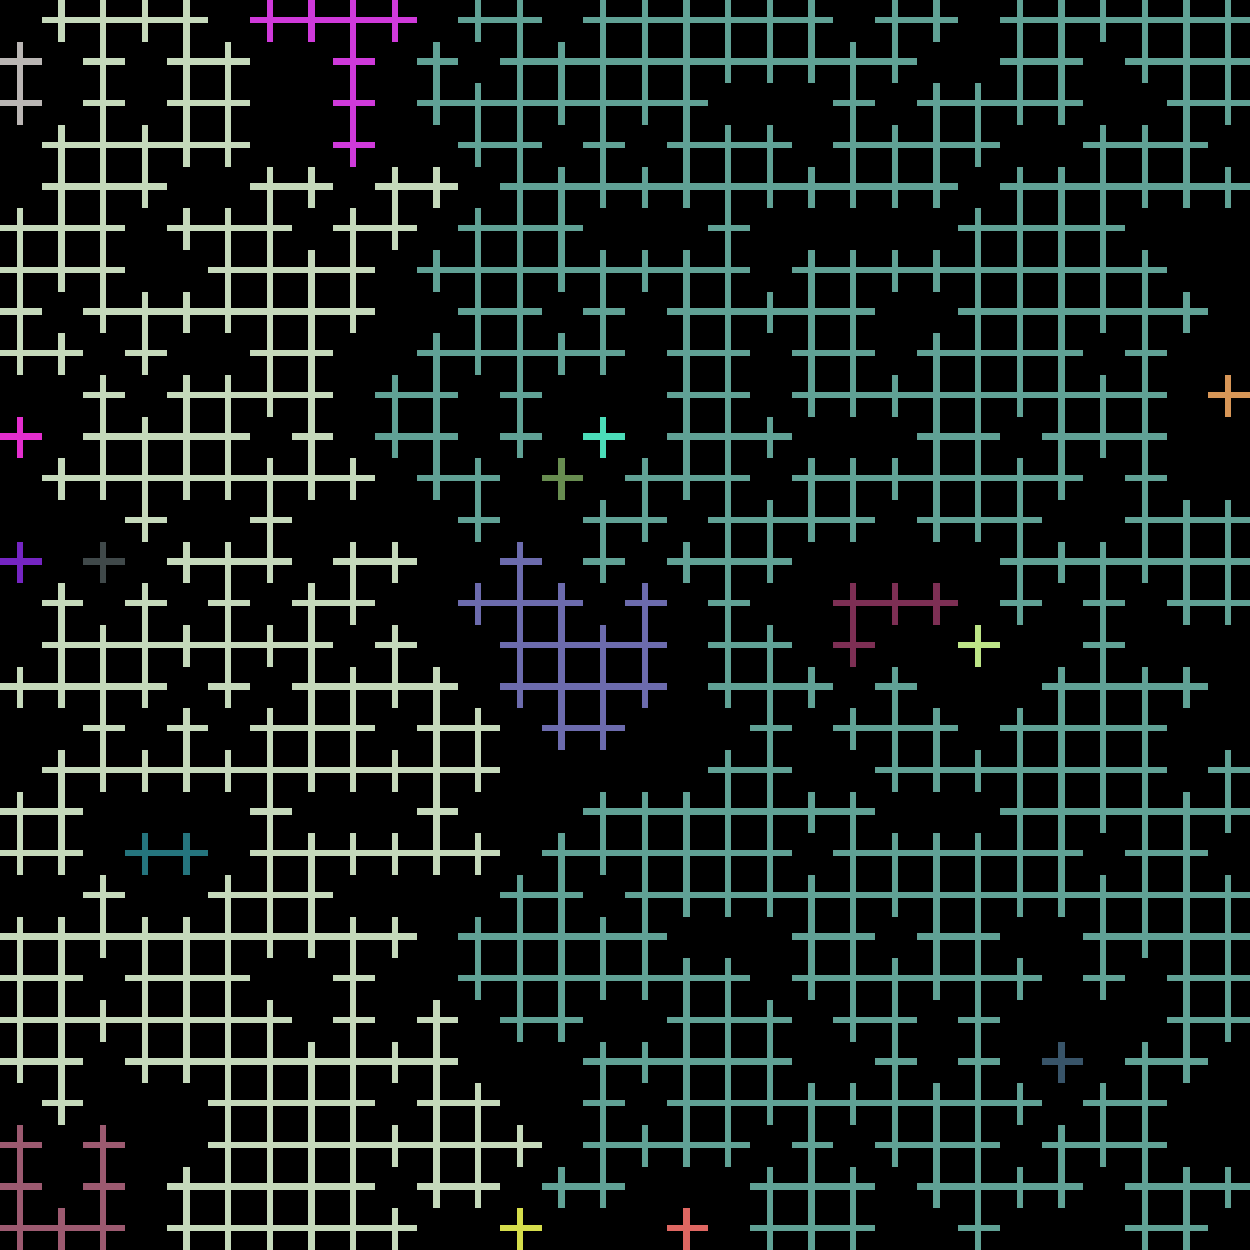
\includegraphics[clip=true, width=0.325\textwidth]{percolation_2}
	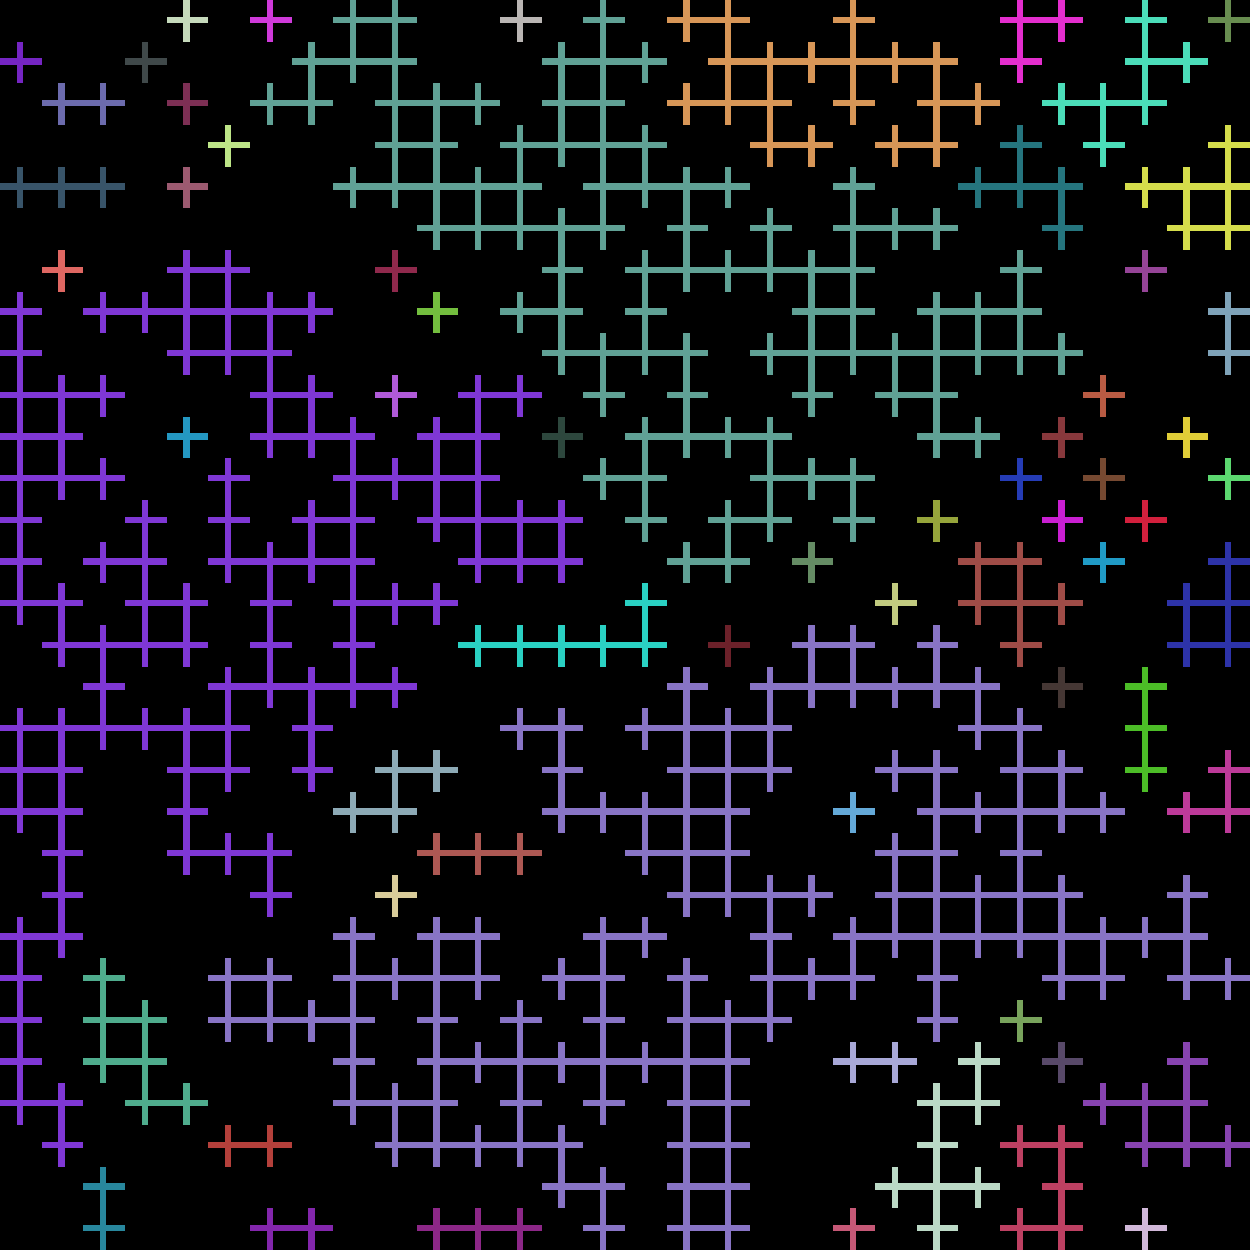
\includegraphics[clip=true, width=0.325\textwidth]{percolation_3}
	\captionspacefig \caption{A square lattice graph subject to different percolation rates (node defects). As the failure rate increases (left to right), the larger network segregates into a multipartite graph of smaller disjoint islands (denoted by colour).} \label{fig:perc_graph}\index{Percolation topologies}
	\end{figure*}
\fi

%
% Random
%

\subsection{Random}\index{Random topologies}

We refer to a random graph as being one in which edges between each pair of vertices occur with some probability $p_\mathrm{edge}$. No vertices are removed from the network, although some may have order \mbox{$|v|=0$}, i.e \mbox{$p_\mathrm{vertex}=1$}. This can be thought of as the edge percolation graph of the complete graph $K_{|V|}$. Some examples are shown in Fig.~\ref{fig:random_graph}.

\if 2\pubmode
	\begin{figure}[!htbp]
	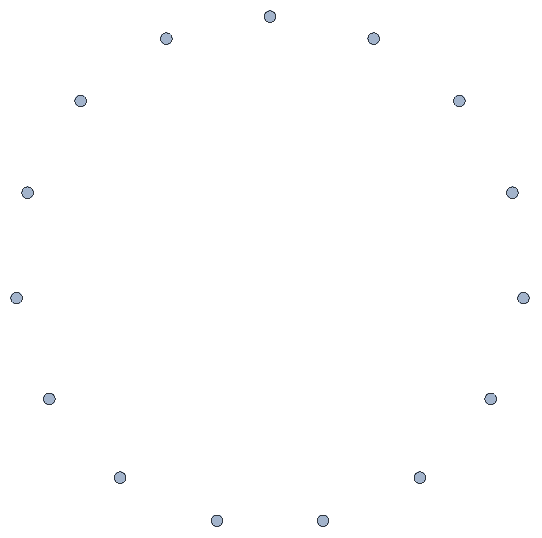
\includegraphics[clip=true, width=0.325\textwidth]{random_0}\\
	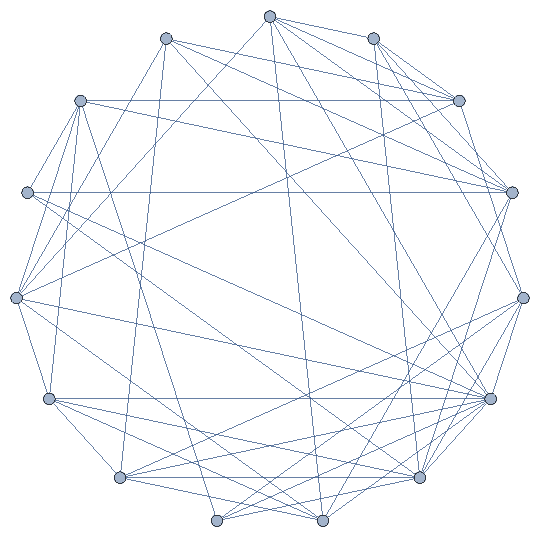
\includegraphics[clip=true, width=0.325\textwidth]{random_05}\\
	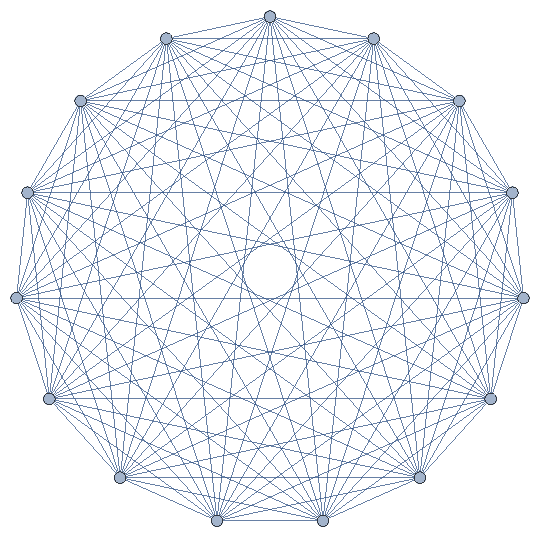
\includegraphics[clip=true, width=0.325\textwidth]{random_1}
	\captionspacefig \caption{The 15-vertex random graph. This is the same as $K_{15}$ in Fig.~\ref{fig:complete_graph}, but where edges are present with probabilities \mbox{$p_\mathrm{edge}=0,0.5,1$} (top to bottom).} \label{fig:random_graph}\index{Random topologies}
	\end{figure}
\else
	\begin{figure*}[!htbp]
	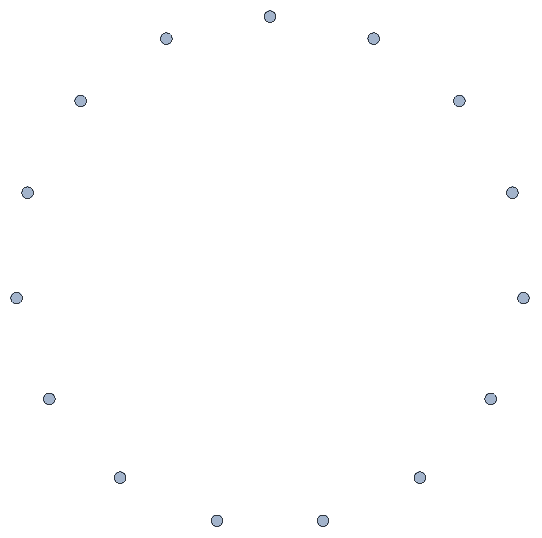
\includegraphics[clip=true, width=0.325\textwidth]{random_0}
	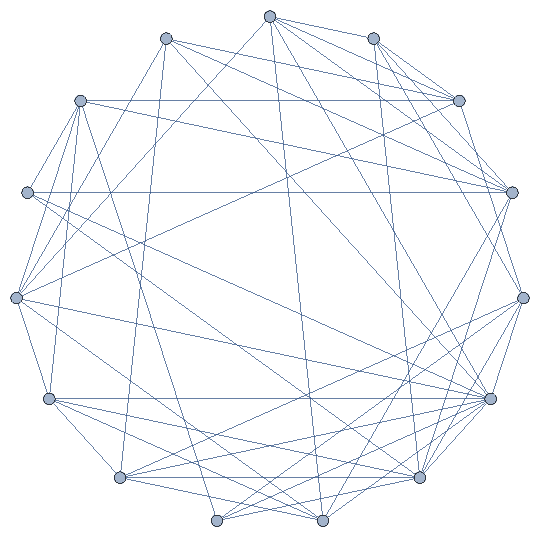
\includegraphics[clip=true, width=0.325\textwidth]{random_05}
	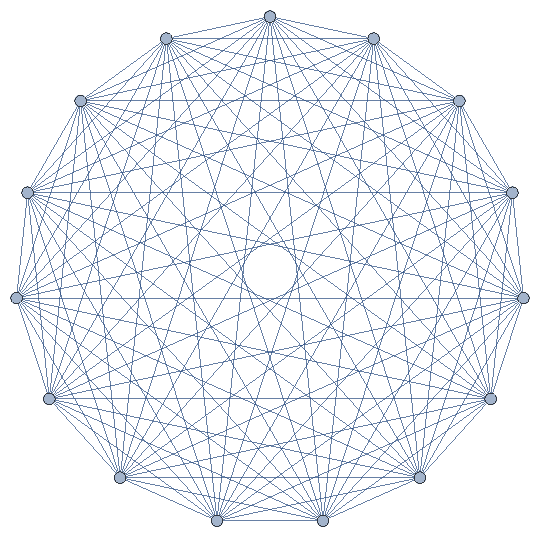
\includegraphics[clip=true, width=0.325\textwidth]{random_1}
	\captionspacefig \caption{The 15-vertex random graph. This is the same as $K_{15}$ in Fig.~\ref{fig:complete_graph}, but where edges are present with probabilities \mbox{$p_\mathrm{edge}=0,0.5,1$} (left to right).} \label{fig:random_graph}\index{Random topologies}
	\end{figure*}
\fi

%
% Hybrid
%

\subsection{Hybrid} \index{Hybrid topologies}

Real networks are highly unlikely to fit the exact form factor of any of the classes of graphs presented above. Rather, a truly global internet is inevitably going to comprise many subnetworks, each structured completely independently of one another, with little consistency or large-scale planning between them. Who thinks about the broader structure of the global internet when setting up their office network?

For example, at the global scale, it is entirely plausible that the internet might take on a random tree-like structure. But when we get down to a lower level, the tree structure vanishes and is replaced by all manner of different network topologies, run and maintained by different organisations in their own distinct ways.

Furthermore, the real-world internet is not simply a hierarchy of different types of well-known graph structures. Rather, it takes the form of `glued' graphs, whereby networks running over different mediums, or via different operators, each exhibit their own independent graph topologies, meeting at interconnect points that join the different networks. Typically this yields redundancy in the routes between different nodes, ushering in the need for combinatorial optimisation techniques when allocating network resources.

This hybrid network topology is the norm today in our classical internet, and it is entirely foreseeable that a similar trend will emerge in the future quantum internet as quantum technologies become more mainstream, their networking less well structured, and competing, redundant links are in place.

%
% Scale-Free Networks
%

\subsection{Scale-free networks}\index{Scale-free networks}\label{sec:scale_free_networks}

Scale-free networks are not defined as obeying a specific topological structure, but rather as following a particular statistical distribution in the connectedness of their nodes. Specifically, the probability distribution function\index{Probability distribution function} for the order of vertices (degree distribution\index{Degree distribution}) roughly follows a Pareto distribution or power law\index{Power law},
\begin{align}\label{eq:pareto_dist}
	P(k) \sim k^{-\gamma},
\end{align}
where $P(k)$ is the probability of a vertex having order $k$ (up to normalisation), and \mbox{$\gamma>1$}. Most commonly \mbox{$2\leq\gamma\leq 3$}. Fig.~\ref{fig:power_law} illustrates this scaling behaviour for different power coefficients.

\begin{figure}[!htbp]
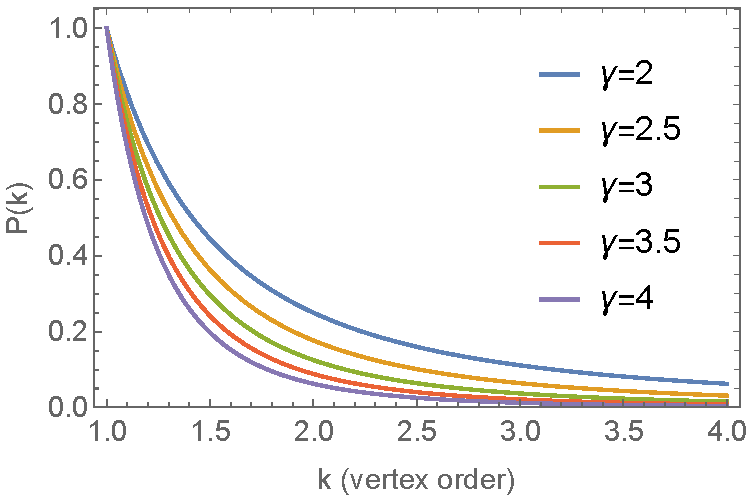
\includegraphics[clip=true, width=0.475\textwidth]{power_law}
\captionspacefig \caption{Examples of the power law, characteristic of the vertex order distribution in scale-free networks.}\label{fig:power_law}\index{Scale-free networks}\index{Power law}	
\end{figure}

This distribution is observed empirically in many real-world networks and sociological structures, and as such is more an observation about the typical behaviour of naturally occurring and evolving human-made networks than an explicit definition for their construction. However, owing to this particular statistical behaviour, and the underlying causations for their Pareto distribution, much has been researched and is known about the properties of scale-free networks.

Scale-free networks arise naturally in systems exhibiting \textit{preferential attachment}\index{Preferential attachment}, i.e when a new node is added to the system it preferentially attaches to nodes that are already more highly connected. This yields a so-called \textit{fitness model}\index{Fitness model}.

According to the Bianconi-Barab{\'a}si fitness model\index{Bianconi-Barab{\'a}si fitness model} \cite{bib:BBfitness, bib:BAfitness}, let \mbox{$\eta_i>0$} be the \textit{fitness factor}\index{Fitness factors} of node $i$, which follow a distribution $\rho(\eta)$, a characteristic of the network. Then the fitness parameters\index{Fitness parameters} are defined to be normalised such that,
\begin{align}
\Pi_i = \frac{\eta_i k_i}{\sum_j \eta_j k_j}.	
\end{align}
Upon adding a new node of degree $m$ to the network, the temporal dynamics will satisfy,
\begin{align}
\frac{\partial P(k_i)}{\partial t}= m\Pi_i.	
\end{align}
The probability distribution can then be shown to have solution,
\begin{align}
P(k) \approx \int \rho(\eta)\frac{C}{\eta}\left(\frac{m}{k}\right)^\frac{C}{\eta+1}\,d\eta,
\end{align}
where,
\begin{align}
	C &= \int \frac{\rho(\eta)\cdot\eta}{1-\beta(\eta)},\nonumber\\
	\beta(\eta) &= \frac{\eta}{C},
\end{align}
which is a linear combination of power law relationships, as required for the definition for scale-free.

Intuitively, why would we expect computer networks (classical or quantum) to be scale-free? To answer this, we simply must establish whether the preferential attachment property will hold. In computer networks there are many reasons why we might expect this to be the case:
\begin{itemize}
	\item Distance\index{Cost vector analysis}: connecting to more highly-connected nodes reduces (on average) the number of channels data packets must traverse to reach their destination, making them `cheaper' in terms of their cost vector analysis (Sec.~\ref{sec:quantum_meas_cost}).
	\item Availability\index{Availability}: larger nodes are more likely to have unused network sockets\index{Sockets} available for use by new nodes. For example, one is more likely to be able to successfully sign up for an internet connection with a major national ISP than a small, local upstart player.
	\item Economies of scale\index{Economies of scale}: the dollar cost per connection of a larger node is likely to be less than for a smaller one, owing to economies of scale. For example, the cost per FLOP of a large-scale supercomputer is far less than for a desktop PC, and Google's data-centres experience lower cost-per-bandwidth on their internet connections than home-users connecting via their ISPs.
\end{itemize}

One notable characteristic of scale-free networks is their hierarchical structure, with a small number of very highly-connected `hubs'\index{Hub nodes} at the top of the food chain, which quickly connect onto smaller hubs, and so on down the food chain with decreasing connectivity.

A feature of scale-free networks of especial interest in the context of computer networks is their robustness against node failure. Suppose we constructed a percolated (Sec.~\ref{sec:perc_topol}) instance of a typical scale-free network. Such a network is highly robust against \textit{random} node/edge deletions compared to many other graph constructions, in the sense that a relatively large number of failures must occur to disconnect the graph. This makes the scale-free network characteristic a particularly attractive one from the perspective of the failure-tolerance of a network. It should be noted that, on the other hand, a scale-free network is highly vulnerable to \textit{targeted} node/edge deletions, that specifically target the highly-connected nodes. A targeted attack against major hubs could disconnect the network with relatively few successful attacks. This brings with it important geo-strategic\index{Geo-strategic politics} considerations when constructing network infrastructure.

Scale-free networks typically exhibit extremely small diameter\index{Graph diameter} (average distance between nodes), scaling as \cite{bib:PhysRevLett.90.058701},
\begin{align}
	d = O(\log \log |V|).
\end{align}
That is, they exhibit (exponentially) smaller diameter than tree graphs (which already exhibit only logarithmic depth). Thus, expanding the network (in a manner consistent with the model) by adding a moderate number of new nodes effectively leaves graph diameter unchanged -- the graph diameter is virtually a constant under modest evolution.

%
% The Internet Web-Graph
%

\subsection{The internet web-graph} \index{Internet web-graph}

Of course, all the topological structures described until now are in-principle constructs. Of most relevance is the \textit{internet web-graph}, the graph of the actual internet (or some other real-world network).

Fig.~\ref{fig:webgraph} illustrates some example web-graphs, constructed from subsets of data from the actual internet. The combination of random, densely and sparsely connected, and tree structures, and its clear hierarchy are all evident. This encourages our intuition of the different types of structures present in realistic networks.

\if 2\pubmode
	\begin{figure}[!htbp]
	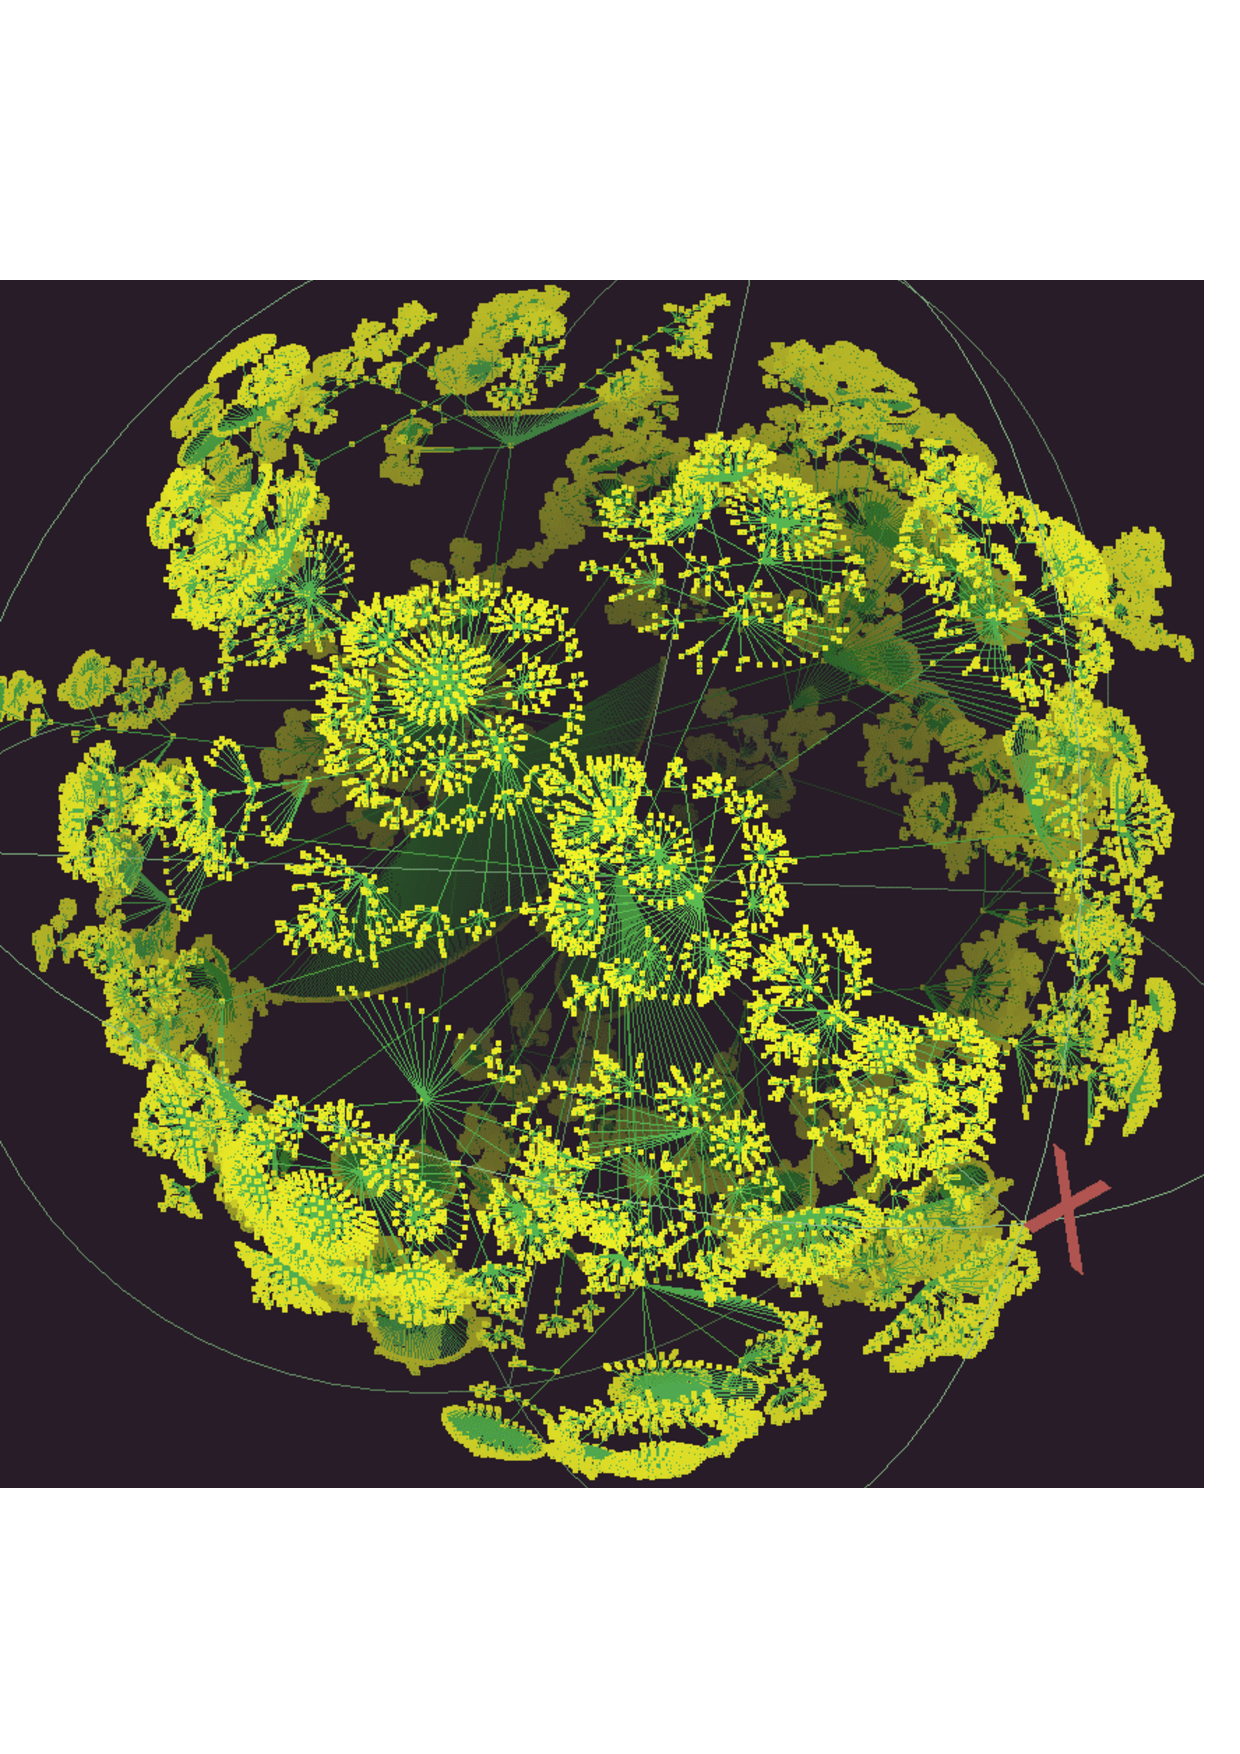
\includegraphics[clip=true, width=0.475\textwidth]{webgraph_1}\\
	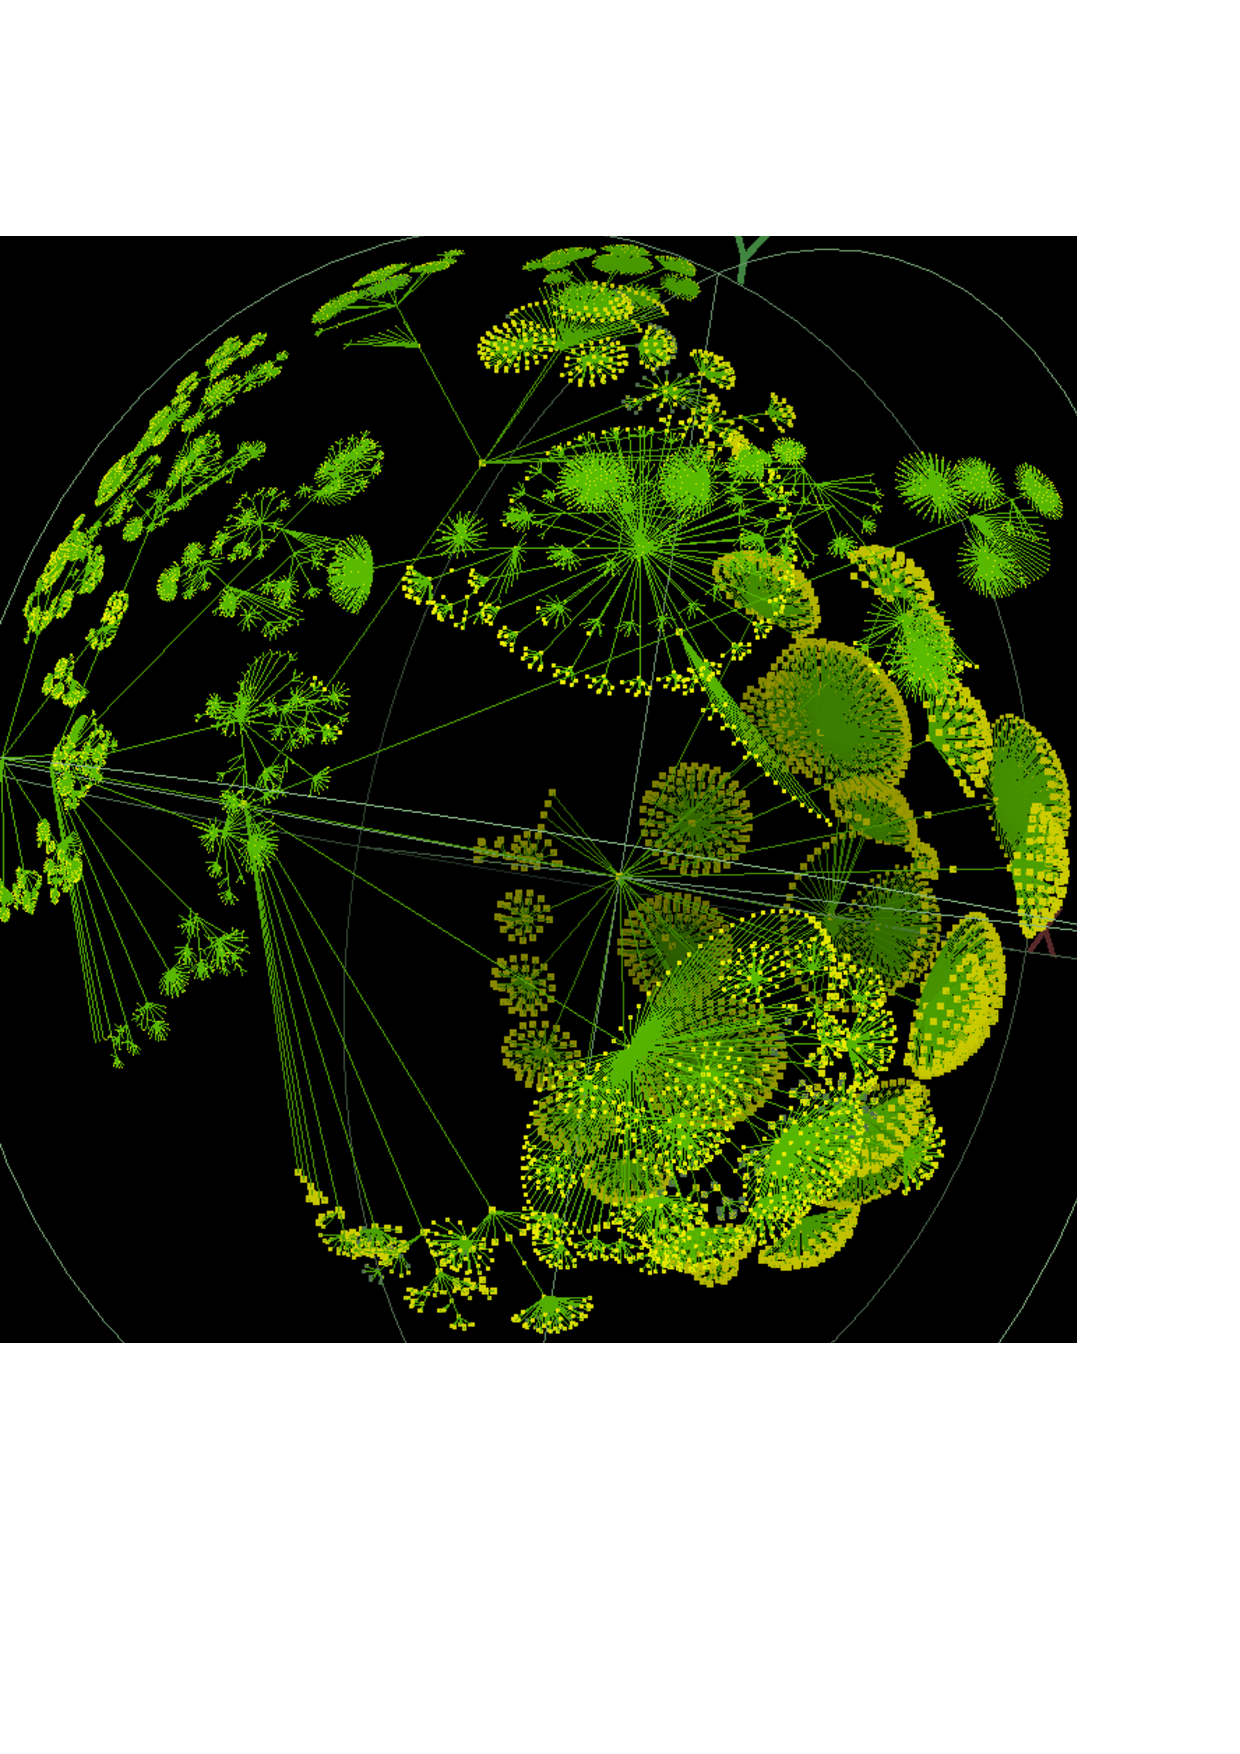
\includegraphics[clip=true, width=0.475\textwidth]{webgraph_2}
	\captionspacefig \caption{Examples of real-world web-graphs of the internet, capturing their high-level random tree-like structure. Graphics attributed to the Center for Applied Internet Data Analysis (CAIDA), \href{http://www.caida.org}{http://www.caida.org}.}\index{Internet web-graph} \label{fig:webgraph}
	\end{figure}
\else
	\begin{figure*}[!htbp]
	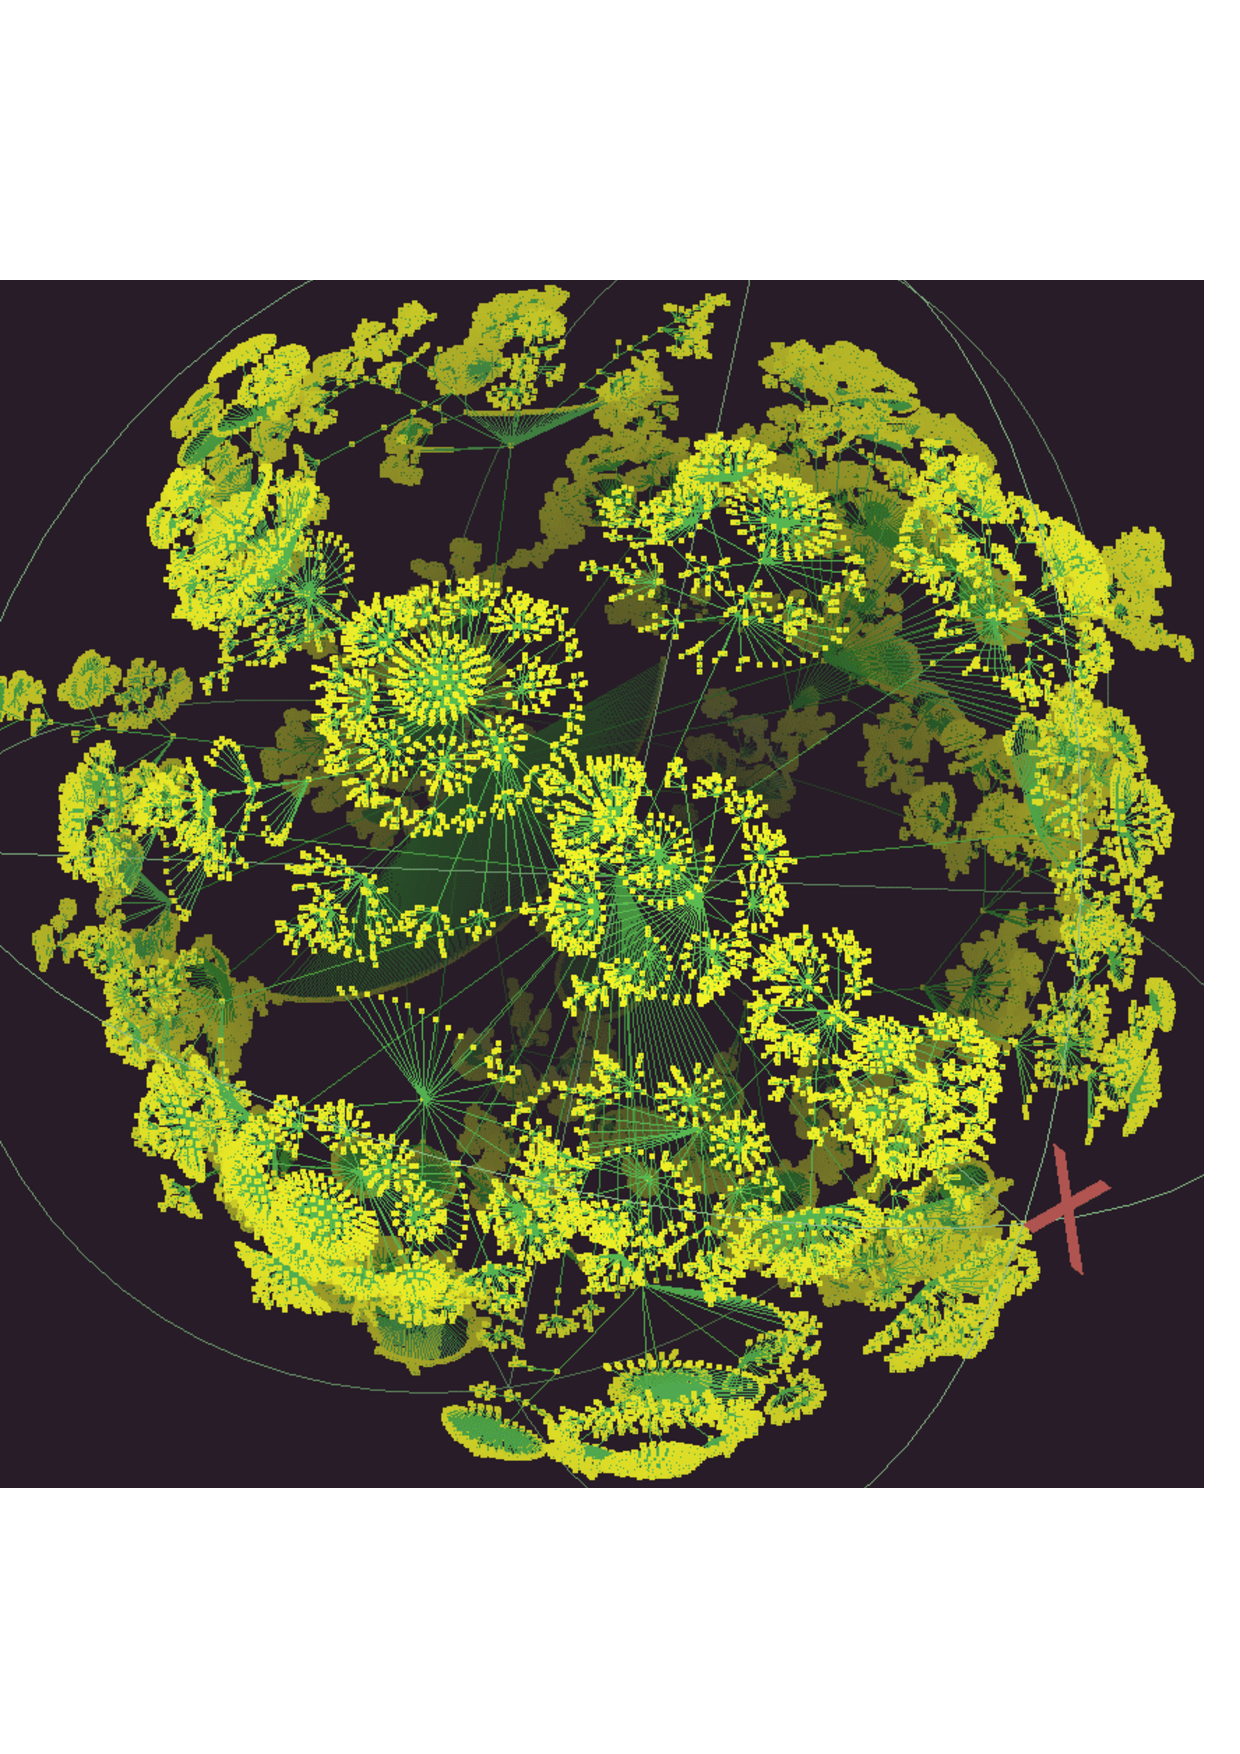
\includegraphics[clip=true, width=0.481\textwidth]{webgraph_1}
	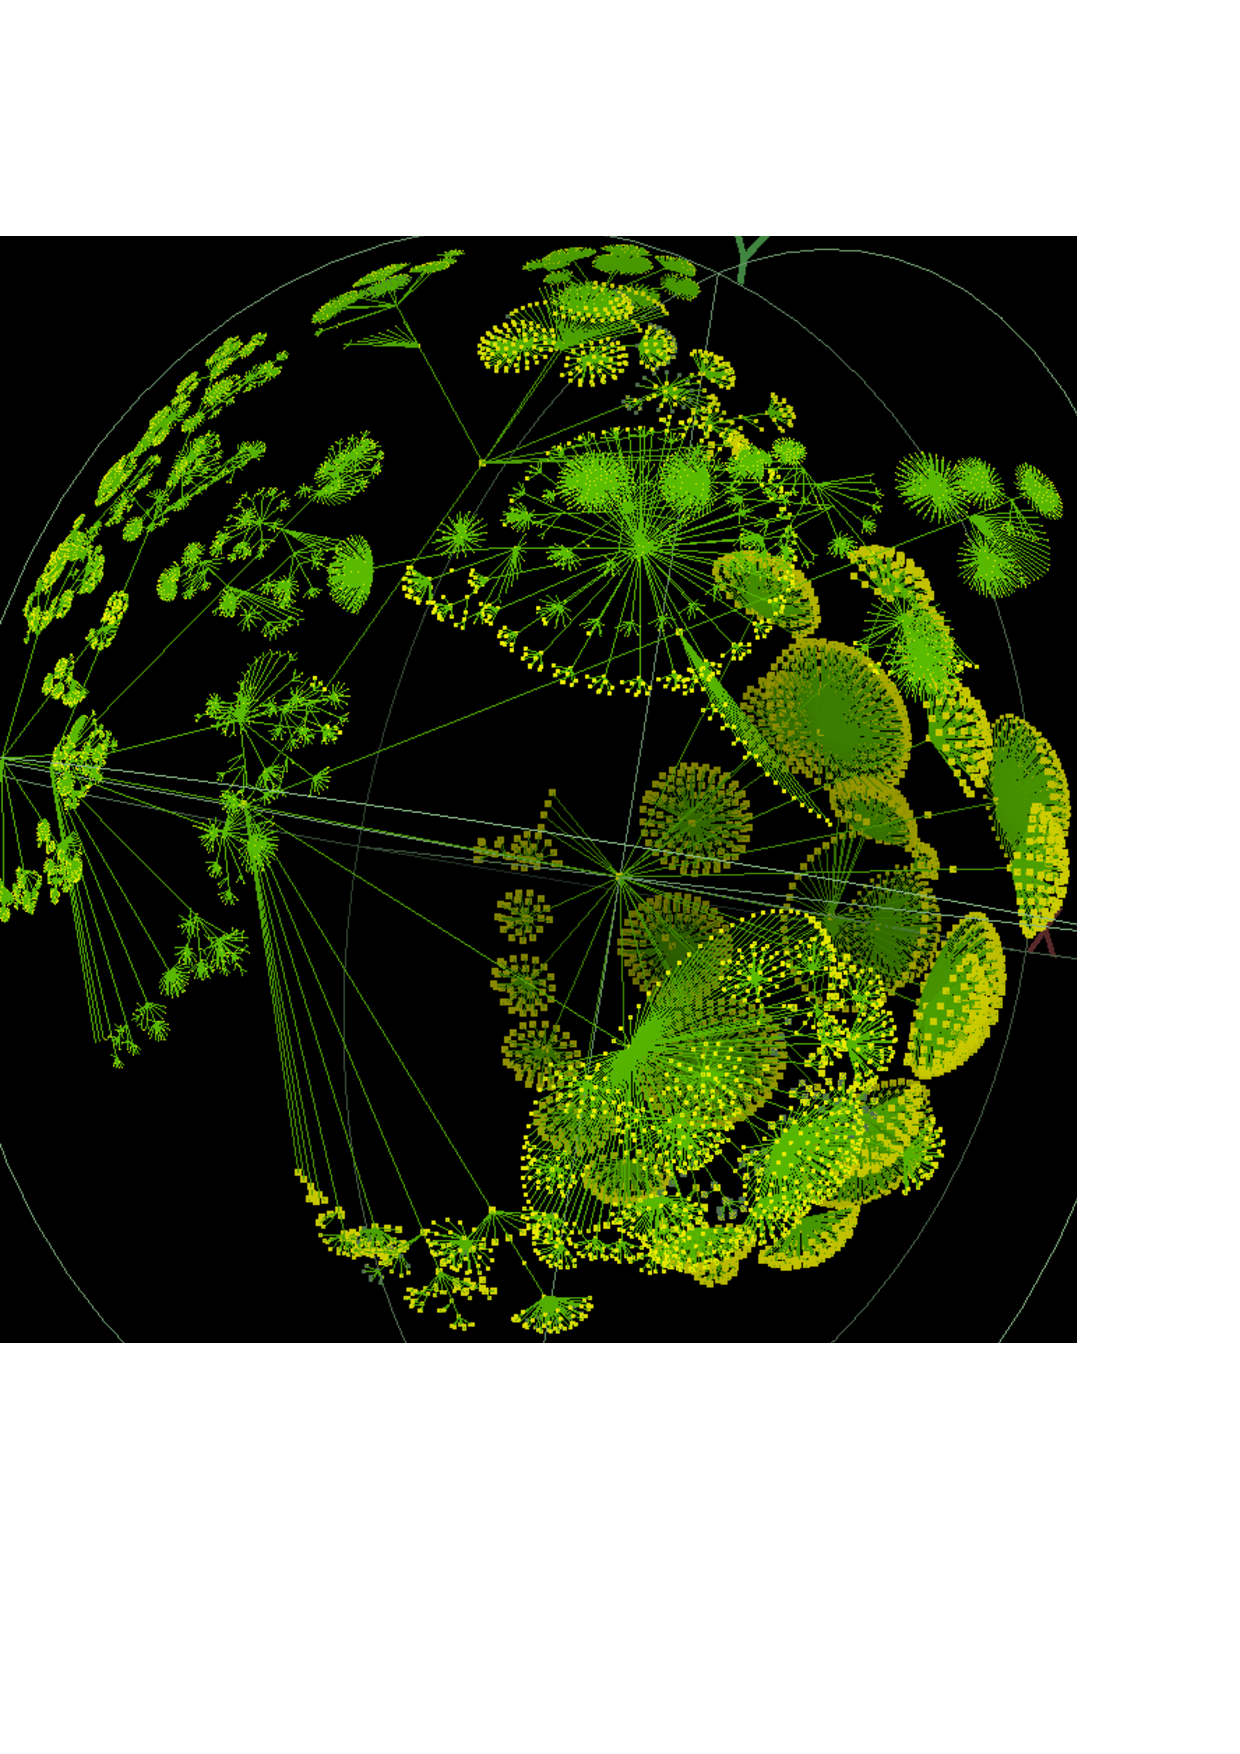
\includegraphics[clip=true, width=0.475\textwidth]{webgraph_2}
	\captionspacefig \caption{Examples of real-world web-graphs of the internet, capturing their high-level random tree-like structure. Graphics attributed to the Center for Applied Internet Data Analysis (CAIDA), \href{http://www.caida.org}{http://www.caida.org}.}\index{Internet web-graph} \label{fig:webgraph}
	\end{figure*}
\fi

The internet web-graph has been observed to be a scale-free network (Sec.~\ref{sec:scale_free_networks}), observing its power law distribution in node connectivity, as per Eq.~(\ref{eq:pareto_dist}).

%
% Network Robustness
%

\subsection{Network robustness}\index{Network robustness}

A key feature of any network topology is its robustness against node or channel failures. This is important from the perspective of naturally occurring hardware faults, and also from a geo-strategic perspective, where adversaries may be launching attacks against the network. In general, there are two main contributing factors to network robustness:
\begin{itemize}
	\item Redundancy\index{Redundancy}: the number of redundant paths between two points in a graph stipulates how many backups there are to finding a route to a destination in the advent of one route failing.
	\item Diameter\index{Diameter}: the chance of a data packet encountering a faulty node/channel increases with the number of hops required to the reach its destination. Graphs with smaller diameter are hence less vulnerable.
\end{itemize}

The extreme case of network robustness is the complete graph, $K_n$, which has P2P links between every pair of nodes. Therefore, if a single channel fails, there are \textit{always} alternate paths taking us between nodes. On the opposing extreme are tree graphs, which contain no redundancy whatsoever, and just a single failure will disconnect the network, making certain routes impossible. Scale-free networks sit in the intermediate zone, but are relatively robust against the failure of random nodes/links, but are vulnerable to conspiratorial failures, which target the elite, highly connected hub-nodes\footnote{The 1\%.}.

Fig.~\ref{fig:graph_deletions} illustrates some examples of these two extreme cases.

\if 2\pubmode
	\begin{figure}[!htbp]
	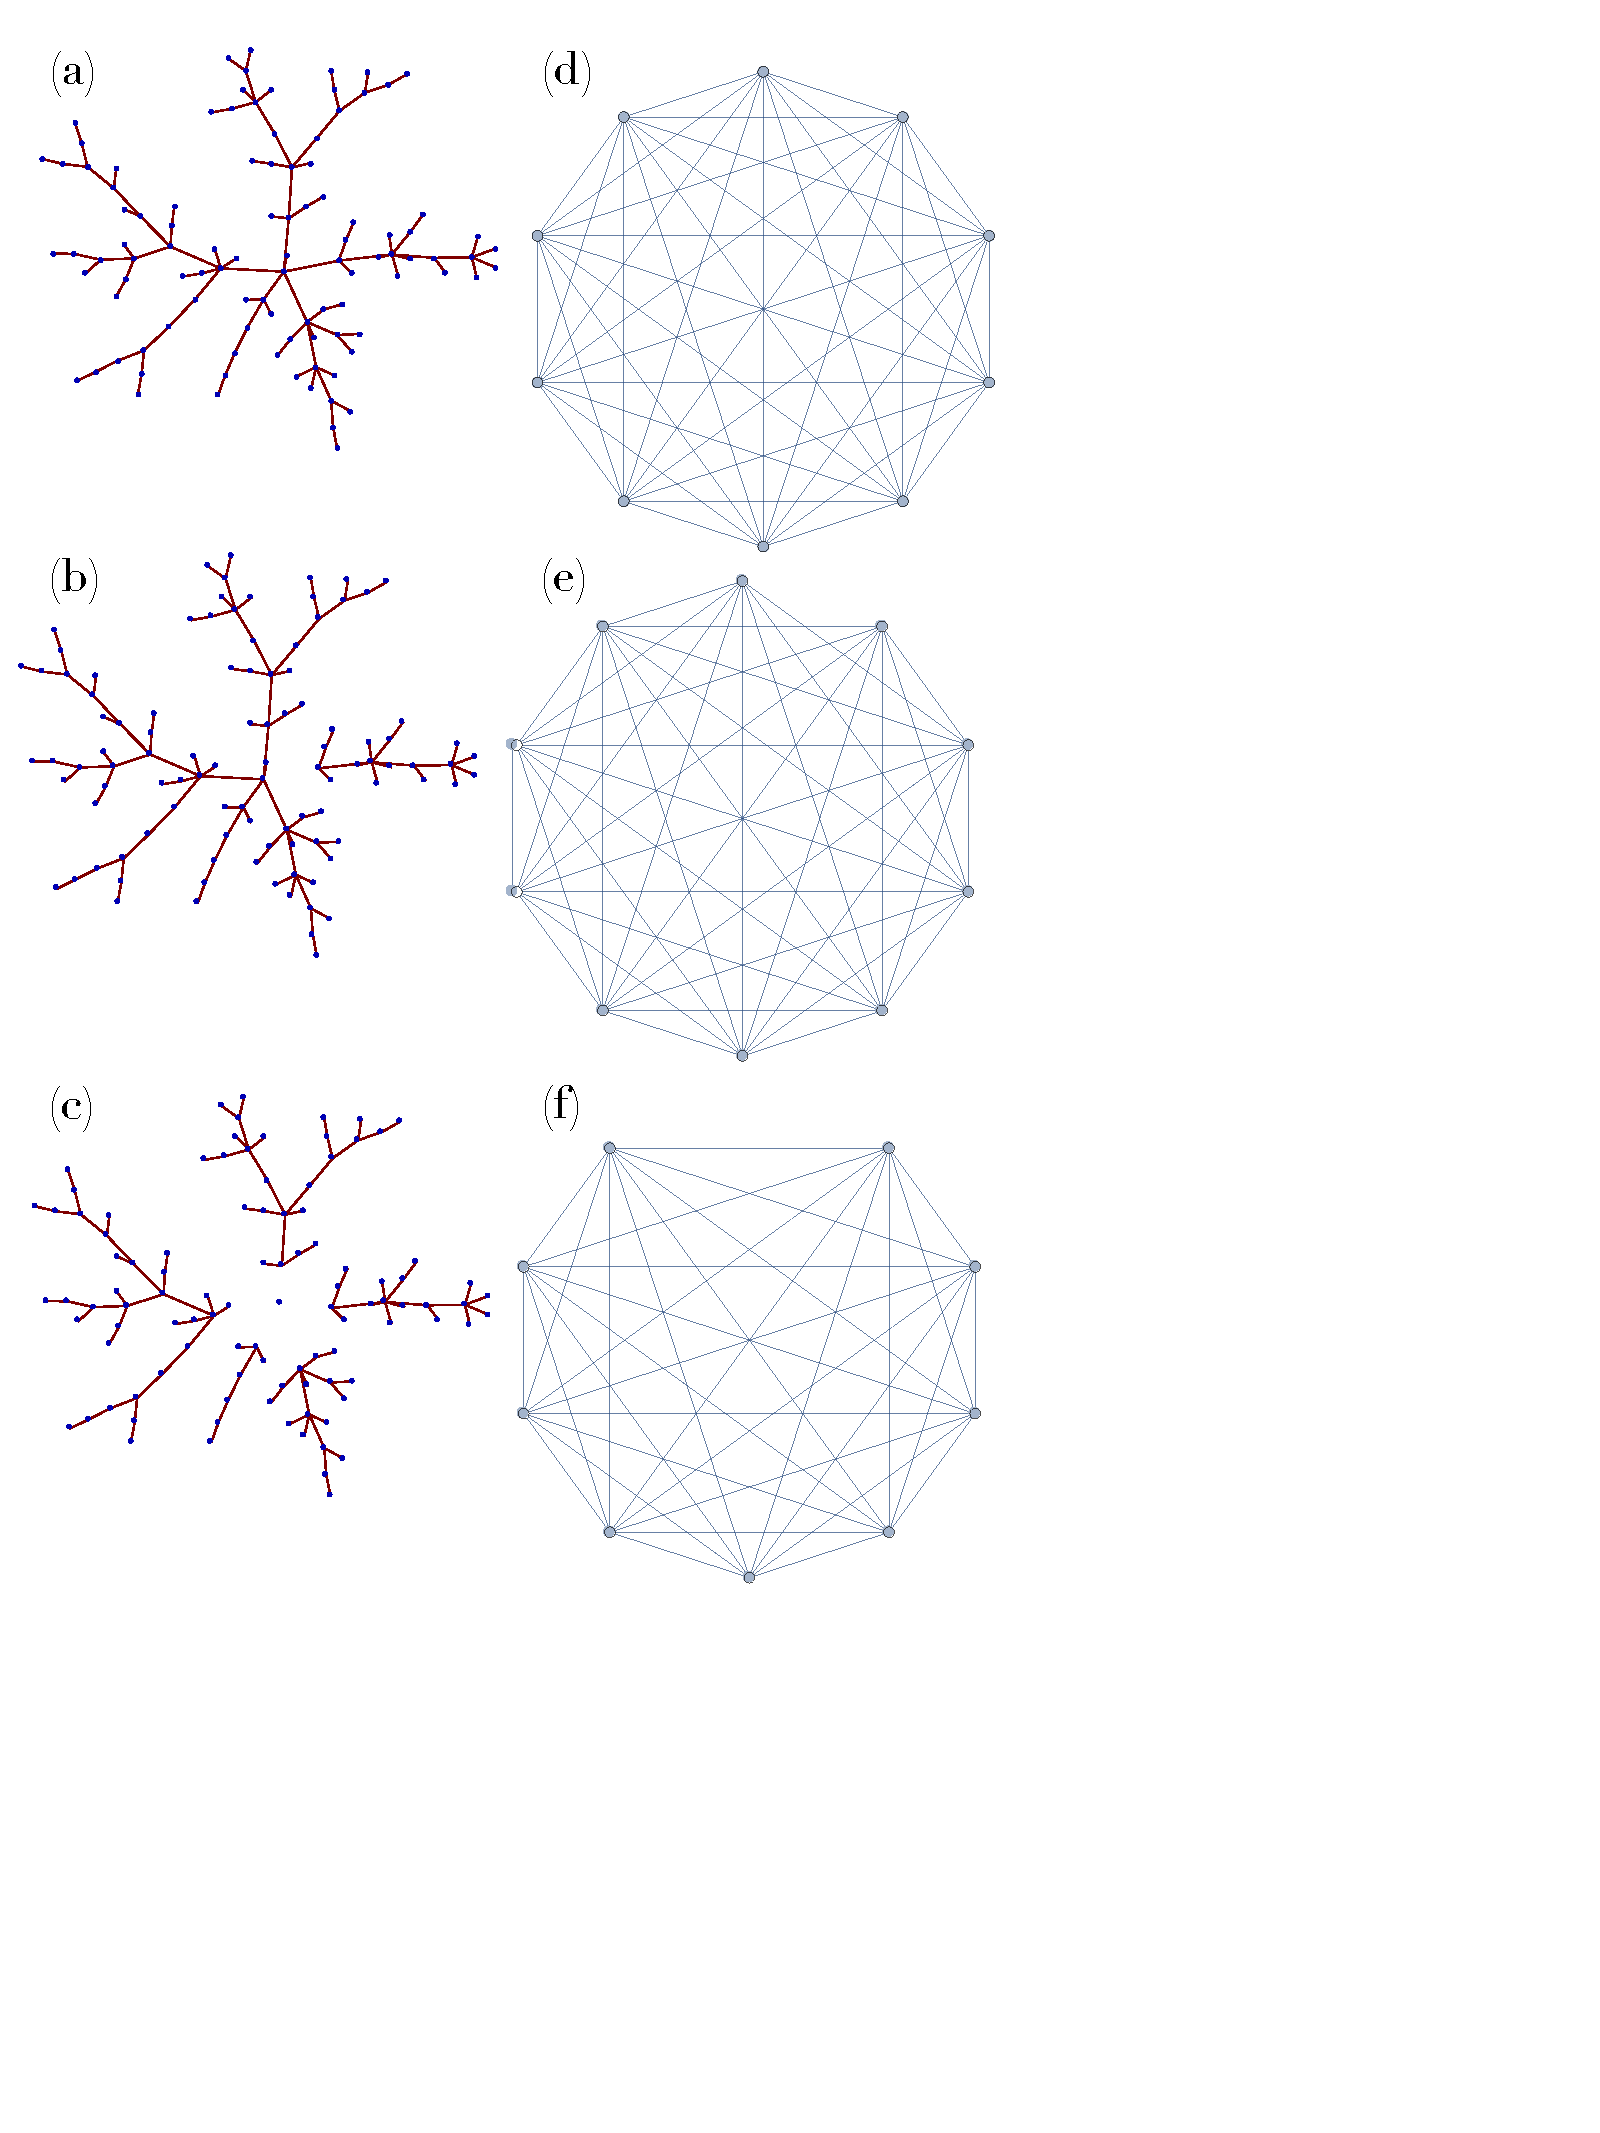
\includegraphics[clip=true, width=0.475\textwidth]{graph_deletions_long}
	\captionspacefig \caption{Robustness of network topologies to node and link deletion. Examples of a tree graph (a) and a complete graph, $K_n$, with \mbox{$n=10$} (d). (b,e) The same graphs subject to a single link failure. The failure disconnects the tree graph into a bipartite graph (b), whereas the complete graph's connectivity is unhindered as alternate routes exist between all nodes (e). A single node failure disconnects the tree graph into a $|v|$-partite graph (c), where $|v|$ is the order of the vertex at which failure occurs. The complete graph, on the other hand, is simply reduced to a $K_{n-1}$ graph, with no loss of connectivity (f). Thus, tree graphs are the most vulnerable network topologies to node/link failures, whereas complete graphs are the most robust.}\label{fig:graph_deletions}
	\end{figure}
\else
	\begin{figure*}[!htbp]
	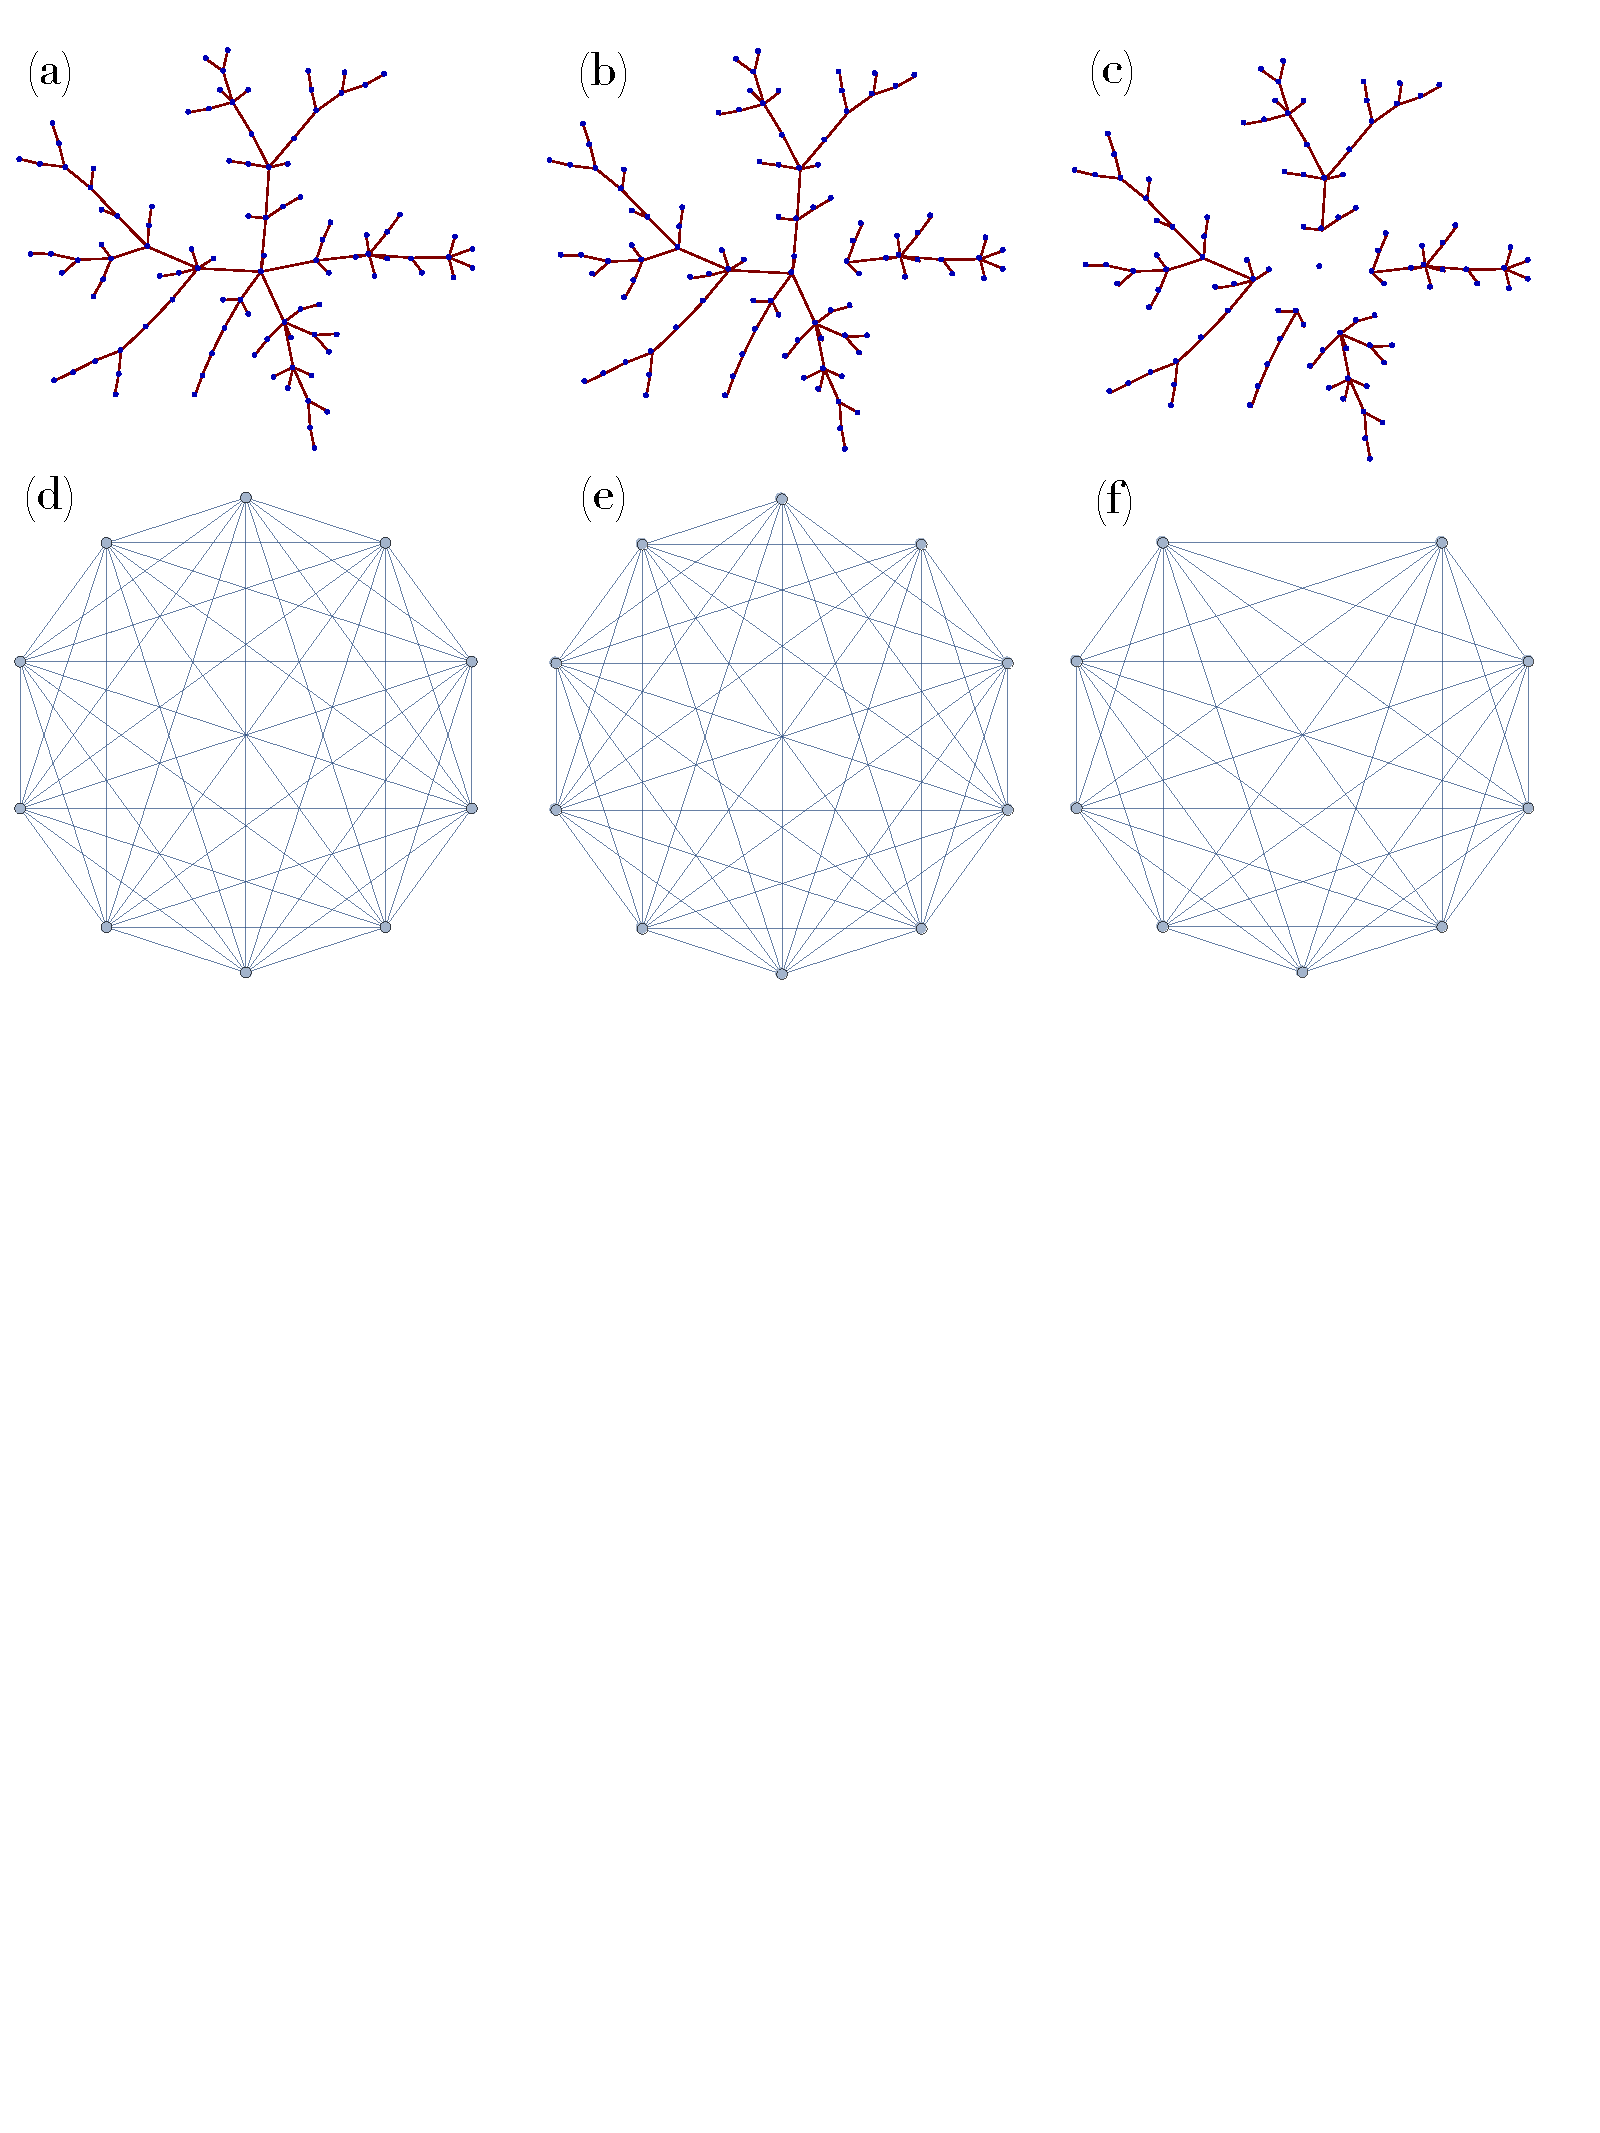
\includegraphics[clip=true, width=\textwidth]{graph_deletions}
	\captionspacefig \caption{Robustness of network topologies to node and link deletion. Examples of a tree graph (a) and a complete graph, $K_n$, with \mbox{$n=10$} (d). (b,e) The same graphs subject to a single link failure. The failure disconnects the tree graph into a bipartite graph (b), whereas the complete graph's connectivity is unhindered as alternate routes exist between all nodes (e). A single node failure disconnects the tree graph into a $|v|$-partite graph (c), where $|v|$ is the order of the vertex at which failure occurs. The complete graph, on the other hand, is simply reduced to a $K_{n-1}$ graph, with no loss of connectivity (f). Thus, tree graphs are the most vulnerable network topologies to node/link failures, whereas complete graphs are the most robust.}\label{fig:graph_deletions}
	\end{figure*}
\fi
\sketch{sketch_21}

\latinquote{Vitam regit fortuna, non sapientia.}

%
% Network Algorithms
%

\section{Network algorithms} \label{sec:graph_theory} \index{Network algorithms}

\dropcap{H}{aving} introduced some of the more relevant graph structures, we now introduce some of the key graph-theoretic algorithms of direct relevance to networking theory \cite{bib:RivestAlgBook}. In graph theory, many fundamental problems are believed to be computationally hard to solve, often \textbf{NP}-complete\index{NP \& NP-complete}. However, there are several important graph algorithms that are (very) classically efficient to solve, and which are of great utility to us as network architects.

We will focus heavily on combinatorial optimisation techniques, where the goal is to allocate network resources so as to optimise some cost metric. This includes both single- and multi-user algorithms, the latter being the far more relevant ones in the context of shared networks like the internet.

In Table.~\ref{tab:net_alg_sum} we summarise the upcoming discussion on important network algorithms, and their associated complexities.

\startnormtable
\begin{table*}[!htbp]
	\begin{tabular}{|c|c|c|c|}
		\hline
  		\rowcolor{Dandelion} Algorithm & Description & Complexity class & Scaling \\
  		\hline
  		\hline
  		\rowcolor{LimeGreen} Breadth-first-search & Explore all vertices in a graph & \textbf{P} & $O(|V|+|E|)$ \\
  		\hline
  		\rowcolor{LimeGreen} Depth-first-search & (same as above) & \textbf{P} & $O(|V|+|E|)$ \\
		\hline
  		\rowcolor{LimeGreen} Shortest-path (Dijkstra) & Find the shortest route between two nodes & \textbf{P} & $O(|V|^2)$ \\
  		\rowcolor{LimeGreen} & in a directed graph & &  \\
  		  		\hline
		\rowcolor{LimeGreen} Shortest-path (\textit{A*}) & (same as above) & \textbf{P} & (varying) \\
  		  		\hline
		\rowcolor{LimeGreen} Single-source shortest path & Find the shortest paths from a given node to & \textbf{P} & $O(|V|\cdot |E|)$\\
  		\rowcolor{LimeGreen} & \textit{all} other nodes & & \\
 		\hline
		\rowcolor{LimeGreen} Minimum spanning tree & Find a spanning tree of a graph that minimises & \textbf{P} & $O(|E|\log |V|)$ \\
  		\rowcolor{LimeGreen} & the total of the edge weights & & \\
  		\hline
  		\rowcolor{LimeGreen} Minimum cost flow & Minimise total costs in a network &  \textbf{P} & $O(|V|\log |V|(|E|$\\
  		\rowcolor{LimeGreen} (Orlin) & with a specified amount of flow& & $+|V|\log |V|))$ \\
  		\hline
  		\rowcolor{LimeGreen} Maximum flow & Maximise flow in a network, regardless of costs & \textbf{P} & $O(|E|\cdot c_\mathrm{max})$ \\
  		\rowcolor{LimeGreen} (Ford-Fulkerson) & & & \\
  		\hline
  		\rowcolor{Lavender} Multi-commodity flow & Same as maximum flow, but generalised to & \textbf{NP}-complete & ? \\
  		\rowcolor{Lavender} & arbitrary numbers of users & (exactly), & \\
  		\rowcolor{Lavender} & & \textbf{P} (approximation & \\
  		\rowcolor{Lavender} & & using heuristics) & \\
  		\hline
  		\rowcolor{Lavender} Vehicle routing problem & Generalises the shortest-path algorithm to multiple & \textbf{NP}-complete & ? \\
  		\rowcolor{Lavender} & users, with distinct sources and destinations & & \\ 
  		\hline
  		\rowcolor{Lavender} Vehicle rescheduling problem & Same as above but with dynamically changing costs & \textbf{NP}-complete & ? \\
    	\hline
	\end{tabular}
	\captionspacetab \caption{Summary of some important network algorithms and their complexities. The \textbf{NP}-complete algorithms are not believed to have efficient classical algorithms, and their exact scaling is not well understood.} \label{tab:net_alg_sum} \index{Network algorithms}\index{Breadth-first-search (BFS) algorithm}\index{Depth-first-search (DFS) algorithm}\index{Shortest-path algorithm}\index{Single-source shortest path algorithm}\index{Minimum spanning tree algorithm}\index{Minimum cost flow algorithm}\index{Maximum flow algorithm}\index{Multi-commodity flow algorithm}\index{Vehicle routing problem}\index{Vehicle rescheduling problem}
\end{table*}
\startalgtable

%
% Network Exploration & Pathfinding
%

\subsection{Network exploration \& pathfinding} \label{sec:path_exp} \index{Network exploration}\index{Pathfinding}

Here the goal is to systematically explore every vertex in an unknown graph exactly once, so as to reconstruct the entire network graph, or to find a target node with unknown location (which can obviously be achieved if the former can be). The two main approaches are \textit{breadth-first-search} (BFS) and \textit{depth-first-search} (DFS) algorithms\index{Breadth-first-search (BFS) algorithm} \index{Depth-first-search (DFS) algorithm}. In both cases we begin at a starting (root) node, from which we wish to explore the entire graph by only following edges to nearest neighbours one at a time.

In BFS we proceed from the root node to visit every one of its neighbours. Having done so, and created a list of those neighbours, we proceed onto the neighbours of the neighbours, and so on, until every vertex in the graph has been visited, or the target node found.

In DFS, on the other hand, we begin by following a single arbitrary path until we reach a dead-end, at which point we backtrack until we reach a branch leading to a vertex we hadn't previously visited.

Examples of these two algorithms are shown in Fig.~\ref{fig:BFS_DFS}.

\if 2\pubmode
	\begin{figure}[!htbp]
	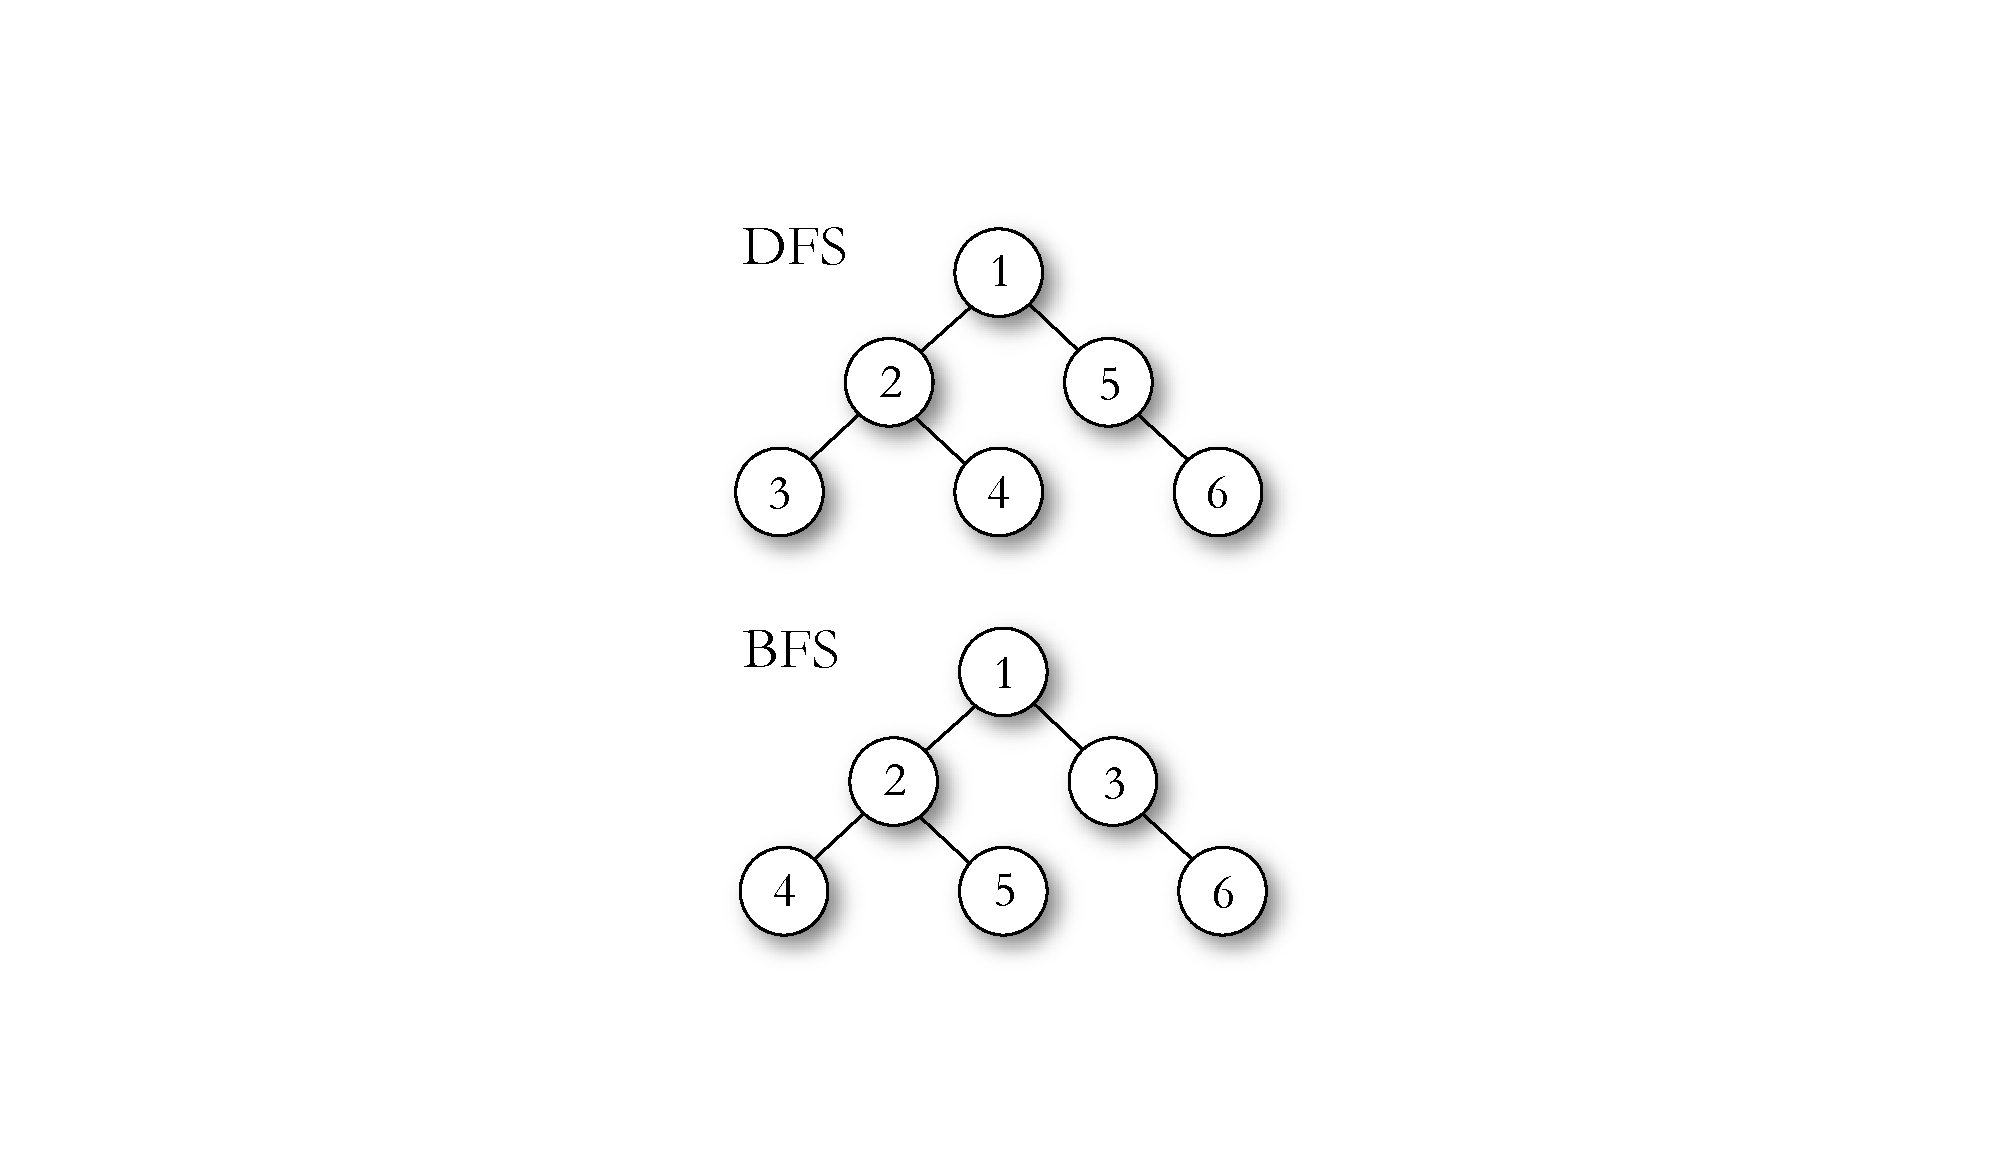
\includegraphics[width=0.3\textwidth]{BFS_DFS_long}
	\captionspacefig \caption{Comparison of the order in which vertices are explored, using the breadth-first-search (BFS) and depth-first-search (DFS) algorithms, where vertex 1 is the root vertex.} \label{fig:BFS_DFS}
	\end{figure}
\else
	\begin{figure*}[!htbp]
	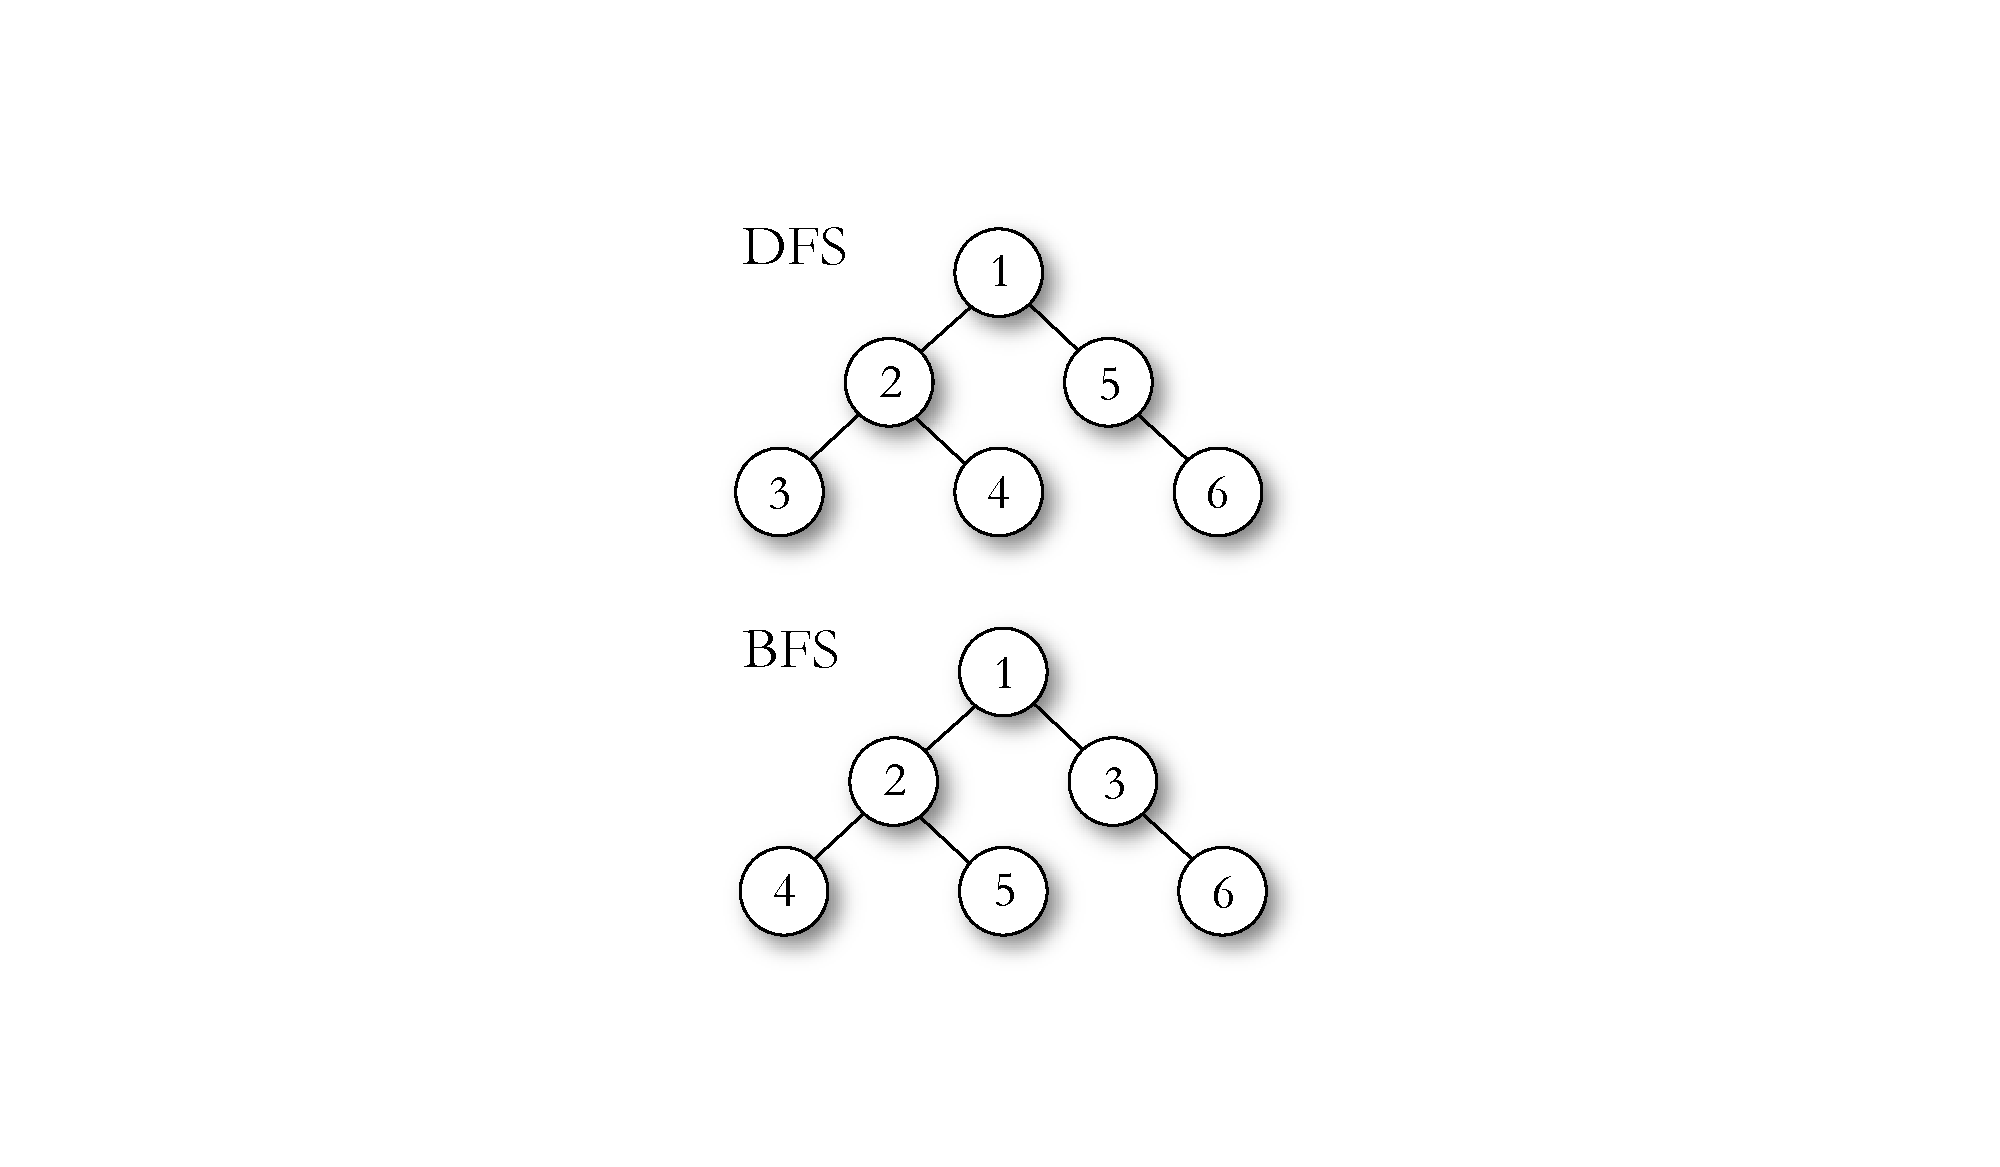
\includegraphics[width=0.65\textwidth]{BFS_DFS}
	\captionspacefig \caption{Comparison of the order in which vertices are explored, using the breadth-first-search (BFS) and depth-first-search (DFS) algorithms, where vertex 1 is the root vertex.} \label{fig:BFS_DFS}
	\end{figure*}
\fi

Both BFS and DFS guarantee visiting every vertex in a connected graph, and do so using only nearest neighbour transitions. Such algorithms are therefore very useful for network discovery.

The BFS algorithm is particularly applicable to pathfinding in ad hoc networks. Consider the situation where there is no central authority with full knowledge of the network, overseeing network operation. Rather, everyone needs to figure things out for themselves by only interrogating their neighbours, to whom they have direct connections. This directly leads to a BFS algorithm, where a node speaks to each of its neighbours in turn, who subsequently do the same thing, yielding a recursive algorithm. This can be naturally parallelised, as each node can be interrogating its neighbours independently, thereby implementing a distributed BFS algorithm. Note that, when searching for a target node, while the BFS algorithm obviously finds the target using the smallest number of hops (i.e a lowest-order route), it needn't necessarily find the route with the lowest cost (which is distinct from the number of hops in general). Shortest-path algorithms require a priori knowledge of the full network graph, discussed in Sec.~\ref{sec:shortest_path}.

Both BFS and DFS exhibit runtime	,
\begin{align}
	O(|V|+|E|),
\end{align}
where $|V|$ and $|E|$ are the number of vertices and edges respectively. Thus, these graph exploration algorithms reside in the complexity class \textbf{P}, and are classically efficient.

%
% Shortest-Path
%

\subsection{Shortest-path} \label{sec:shortest_path} \index{Shortest-path algorithm}

In graph theory, the shortest-path problem is that of finding a subgraph of a given graph $G$, connecting two vertices, \mbox{$A\to B \subset G$}, such that the sum of its edge weights is minimised. In the context of our application to route-finding, this amounts to finding a route that minimises cost.

The first proven shortest-path algorithm was invented by and named after Dijkstra \cite{bib:Dijkstra59}, which requires runtime,
\begin{align}
	O(|V|^2),
\end{align}
also residing in \textbf{P}\index{P} (one of the relatively few, and highly valuable optimisation problems that is classically efficient). Subsequently, a number of improvements and variations on Dijkstra's algorithm have been proposed, most notably the $A^*$ algorithm \cite{bib:Astar}\index{Shortest-path algorithm}, which has found widespread modern use, using a heuristic approach to improve performance over Dijkstra.

Formally, let $\vec{R}$ be the set of all routes \mbox{$A\to B$}. Then,
\begin{align}
c_\mathrm{opt} = \min_{r\in R} \left(\sum_{i\in r} c_\mathrm{net}(i) \right),
\end{align}
where \mbox{$i\in r$} denotes the $i$th edge in the route $r$. Intuitively, the (in general) exponential number of possible paths through a graph might lead one to believe the above optimisation problem is a computationally inefficient one (such as \textbf{NP}-complete, or worse). However, perhaps surprisingly, Dijkstra's algorithm cleverly manages to reduce this to a polynomial-time problem. A sketch of the algorithm is provided in Alg.~\ref{alg:dijkstra}, which needn't be understood by the reader desperate to read further.

\begin{table}[!htbp]
\begin{mdframed}[innertopmargin=3pt, innerbottommargin=3pt, nobreak]
\texttt{
function DijkstraShortestPath($G$,$A$,$B$):
\begin{enumerate}
	\item currentNode = $A$
    \item tentativeDistances[$A$] = 0
    \item tentativeDistances[others] = $\infty$
    \item nodesVisited[$A$] = True
    \item nodesVisited[others] = False
    \item loopStart:
    \item neighbours = currentNode.neighbourhood
    \item nodesVisited[neighbours] = True
    \item for(n$\in$neighbours) \{
    \setlength{\itemindent}{0.2in}
    \item newTentativeDist = \\ min(tentativeDistances[currentNode] \\+ edgeWeight[currentNode,n],\\
        tentativeDistances[n])\\
    \item nodesVisited[currentNode] = True
    \setlength{\itemindent}{0in}
    \item \}
    \item if(nodesVisited[$B$] = True) \{
    \setlength{\itemindent}{0.2in}
	\item return(tentativeDistances[$B$])
	\item $\Box$
    \setlength{\itemindent}{0in}
    \item \}
	\item currentNode = \\
	tentativeDistances[unvisitedNodes].\\
	nodeWithSmallest()
	\item goto(loop)
    \item $\Box$
\end{enumerate}}
\end{mdframed}
\captionspacealg \caption{Dijkstra's original shortest-path algorithm for finding the lowest weight path through a graph, $G$, between two vertices, $A$ (source) and $B$ (destination). The algorithm has $O(|V|^2)$ runtime (in \textbf{P}).} \label{alg:dijkstra}\index{Shortest-path algorithm}
\end{table}

Fig.~\ref{fig:simp_route_opt} illustrates a directed, edge-weighted graph. A shortest-path algorithm applied between vertices $A$ and $B$ would return \mbox{$R_\mathrm{shortest} = A\to F\to B$} as the minimum cost route.

When introducing network graphs earlier, we insisted upon all costs being associated with edges rather than vertices, and presented a trivial means by which to convert vertex costs to edge costs in Fig.~\ref{fig:remove_nodes}. This adamance arose because the presently described shortest-path algorithms operate purely in terms of edge weights, not vertex weights. But the mapping we presented from the latter to the former obviates this issue.

This is the motivating factor behind representing network graphs purely in terms of edge weights (Sec.~\ref{sec:quant_proc_in}), thereby enabling compatibility with shortest-path algorithms.

For the purposes of the QTCP protocol, we are interested in the case of directed graphs (recall that in terms of cost metrics, undirected graphs can be converted to directed graphs by replacing undirected edges with a pair of identical edges in opposite directions).

Shortest-path techniques find widespread application in many areas. Computer networks are an obvious candidate, since networks are inherently graph-theoretic by nature.

To implement the shortest-path algorithms discussed above, the party performing the calculation requires knowledge of the full network graph. In an ad hoc network, where users might be added to or removed from the network arbitrarily, this isn't necessarily the case.

One solution is for a central authority to be responsible for maintaining a ledger of all network participants and their connectivity, which users are required to notify upon joining or leaving the network. The central authority may then apply shortest-path calculations, which may be queried by users. However, a disruption in connection to the central authority, or failure of nodes to notify the central authority upon joining or leaving the network, introduces a point of failure into the operation of the protocol.

Another approach, which does not require a reliable central authority, is for users to implement network exploration algorithms each time they wish to perform a shortest-path calculation. This facilitates truly ad hoc networking, but incurs the cost overhead associated with nodes frequently implementing network exploration. However, network exploration is a purely classical algorithm, which may run entirely over the classical network, and therefore incurs no cost in quantum resources.

With this approach, a new node can join the network, without having to know anything about the topology of the network. Similarly, upon leaving the network, it needn't notify anyone, since a future interrogation by a neighbour will be detected as a non-existent node. The BFS is therefore highly suited to ad hoc operation. In fact, present-day internet gateway protocols (Sec.~\ref{sec:gateway}) essentially implement a distributed version of BFS.

%
% Single-Source Shortest-Path Algorithm
%

\subsection{Single-source shortest-path} \label{sec:single_source_sp} \index{Single-source shortest path algorithm}

The shortest-path algorithm by Dijkstra presented above finds the shortest route between two specified nodes in a network. However, when employing \textsc{Individual} routing strategies, where there is no central mediation of the network, each node desires an up-to-date routing table, showing the best route to take to any other point in the network. Then, upon receiving packets with particular destinations, rather than repeatedly applying Dijkstra's algorithm, we can simply look up the destination on the node's local routing table.

Single-source shortest-path algorithms address this problem by calculating the shortest paths from the current node to \textit{every} other node in the network topology.

The best-known algorithm for this problem is the Bellman-Ford (or Bellman-Ford-Moore)\index{Bellman-Ford-Moore algorithm} algorithm \cite{BF}, which requires worst-case runtime of,
\begin{align}
	O(|V|\cdot |E|).
\end{align}
Clearly this is more complex than Dijkstra's algorithm for finding a particular shortest-path. But it is more efficient than using brute-force to find the shortest-path between every pair of nodes in the network via $O(|V|^2)$ repeated applications of Dijkstra.

%
% Minimum Spanning Tree
%

\subsection{Minimum spanning tree} \label{sec:min_tree} \index{Minimum spanning tree algorithm}

MST algorithms find an MST\footnote{There may be multiple distinct MSTs for a given graph.} of some arbitrary graph. Like the shortest-path problem, it has a polynomial-time, deterministic algorithm (i.e it resides in \textbf{P}\index{P}). The first MST algorithm \cite{bib:Boruvka26} required,
\begin{align}
	O(|E|\log |V|),
\end{align}
runtime. Numerous variations have since been proposed, with little change to the underlying scaling.

Because MST algorithms are efficient, they play a very useful role in the design of real-world network topologies, where resource minimisation is crucial.

Fig.~\ref{fig:mst} shows an example of a graph with its MST.

%
% Minimum Cost Flow
%

\subsection{Minimum cost flow} \label{sec:min_cost_flow_prob} \index{Minimum cost flow algorithm}

The \textit{minimum cost flow problem} \cite{???} is that of minimising costs through a network for a specified amount of flow (i.e total bandwidth or throughput), which acts as a constraint on the problem. The definition of `cost' in this context is compatible with our earlier definition of cost metrics (Def.~\ref{def:metric}).

This problem can be efficiently solved using linear programming. Specifically, cost metrics along links in series are given by linear combinations of individual link costs. If, in addition, we let our net cost function be linear in the constituent costs then the net cost will also be linear in all the edge weights. This lends itself directly to optimisation via linear programming techniques. Algorithms for linear programming, such as the \textit{simplex} algorithm, have polynomial-time solutions (i.e reside in \textbf{P}\index{P}), and a plethora of software libraries are available for implementing them numerically.

One polynomial-time algorithm, by \cite{JAMES_B_ORLIN}, for solving this problem does so in, 
\begin{align}
	O(|V|\log |V|(|E|+|V|\log |V|)),
\end{align}
time.

%
% Maximum Flow
%

\subsection{Maximum flow} \label{sec:max_flow_prob} \index{Maximum flow algorithm}

The \textit{maximum flow problem} \cite{???} is the seemingly simple goal of -- as the name suggests -- maximising network flow, without consideration for any of the other cost metrics or attributes associated with the network. This type of problem is relevant when brute bandwidth is the dominant goal.

This problem can be tackled using a number of techniques. In some circumstances, linear programming techniques can be employed. The best-known algorithm is the Ford-Fulkerson algorithm\index{Maximum flow algorithm} \cite{???}, which finds a solution in,
\begin{align}
	O(|E|\cdot c_\mathrm{max}),
\end{align}
runtime, where $|E|$ is the number of links in the network and $c_\mathrm{max}$ is the maximum cost present in the network. The algorithm behaves pathologically in some conditions, which can easily be overcome in the context we present here. Using Ford-Fulkerson as a starting point, numerous other more sophisticated algorithms have been developed.

%
% Multi-Commodity Flow
%

\subsection{Multi-commodity flow} \label{sec:multi_comm_flow} \index{Multi-commodity flow algorithm}

The \textit{multi-commodity flow problem} \cite{???} generalises the previous algorithms to be applicable to multi-user networks. The generalisation is that there may be a number of distinct senders, residing on different nodes, each transmitting to distinct recipients, residing on different nodes. This is the most realistic scenario we are likely to encounter in a real-world quantum internet, where networks will inevitably be shared by many users, residing at different nodes.

Unfortunately the computational complexity of solving this problem is much harder than the previous algorithms in general. Specifically, solving the problem exactly is \textbf{NP}-complete\index{NP \& NP-complete} in general. However, in specific circumstances it can be approached using linear programming or polynomial-time approximation schemes.

%
% Vehicle Routing Problem
%

\subsection{Vehicle routing problem} \label{sec:VRP} \index{Vehicle routing problem}

The vehicle routing problem (VRP) is a multi-user generalisation of the shortest-path problem, where the goal is to minimise total network cost (i.e the sum of all individual users' costs) when there are multiple users sharing the network, each with distinct sources and destinations.

Unlike the polynomial-time shortest-path algorithm, exactly solving the VRP is \textbf{NP}-hard\index{NP \& NP-complete} in general. However, heuristic methods can find approximate suboptimal solutions far more efficiently, and there is a multitude of software packages available for doing so.

The VRP has found widespread use in, for example, the routing of transport networks for delivery companies or public transportation networks (hence the name), and many commercial companies exist, which perform these kinds of optimisations on behalf of transport providers to enhance their efficiency.

It is obvious that this algorithm is directly applicable to multi-user communications networks, which are conceptually identical to transport networks, albeit a bit faster. 

A multitude of variations on the VRP exist, accommodating for different types of constraints (or additional flexibilities) in the operation of the network.

%
% Vehicle Rescheduling Problem
%

\subsection{Vehicle rescheduling problem} \label{sec:VRSP} \index{Vehicle rescheduling problem}

The vehicle rescheduling problem (VRSP) generalises the VRP to the case where properties of the network undergo changes dynamically within the course of transmissions over the network. To use the analogy of transport networks, this could entail, for example, a truck breaking down en route to its destination, requiring real-time rescheduling of the other vehicles.

Solving the VRSP exactly is \textbf{NP}-complete\index{NP \& NP-complete} in general, but as with the VRP, heuristic methods can often be applied, which efficiently find approximate solutions.

In the context of communications over networks, the VRSP has obvious applicability -- a quantum internet is likely going to be largely ad hoc in nature, with users coming and going, and many non-deterministic points of failure, requiring ongoing updating of routing decisions if resource allocation is to remain as efficient as possible.

%
% Improving Network Algorithms Using Quantum Computers
%

\subsection{Improving network algorithms using quantum computers} \index{Network algorithms on quantum computers}

Given that we are directing this work at the upcoming quantum era, where quantum computing will become a reality, it is pertinent to ask whether quantum computers might improve the aforementioned network algorithms, some of which are computationally hard problems. Most notably, several of the discussed algorithms are \textbf{NP}-complete\index{NP \& NP-complete} in general, a complexity class strongly believed to be exponentially complex on classical computers. Can quantum computers help us out here, and improve network resource allocation? Can quantum computers help themselves?

While it is not believed that quantum computers can efficiently solve such \textbf{NP}-complete\index{NP \& NP-complete} problems, it is known that they can offer a quadratic speedup using Grover's unstructured search algorithm. Specifically, \textbf{NP}-complete\index{NP \& NP-complete} problems can be treated as satisfiability problems, where we are searching for an input to a classical algorithm that yields a particular output.

To gain a quantum advantage, we treat the classical algorithm as an oracle whose input configurations form an unstructured search space. Then, Grover's algorithm can perform a search over the space of input configurations to find a satisfying solution, with quadratically enhanced runtime.

While a quadratic improvement is far short of the exponential improvement we might hope for, Grover's algorithm is known to be optimal for the unstructured search problem \cite{?}. Nonetheless, despite only yielding a quadratic improvement, a quadratic speedup may already be sufficient to significantly improve network resource allocation.
\sketch{sketch_22}

%
% Quantum networks
%

\part{Quantum networks}\label{part:quant_net}\index{Quantum networks}

%
% Quantum Networks
%

\section{Quantum networks} \label{sec:quant_net} \index{Quantum networks}

\dropcap{W}{e} have reviewed some of the key aspects of classical networks, including the real-world implementation of classical networking via the TCP/IP protocol stack, and the essential mathematical foundations for networking theory, including cost vector analysis and routing strategies.

Let us now lay the foundations and some of the key motivations and assumptions we will make in our upcoming discourse on quantum networks, and lay out some of the key differences between classical networks and future quantum ones.

Quantum networks comprise all the same ingredients as classical networks, but with some very important non-classical additions. Nodes can additionally implement quantum computations, quantum-to-classical interfaces (i.e measurements), quantum-to-quantum interfaces (i.e switching data between different physical systems), quantum memories, or any quantum process in general. Many of these are not allowed by the laws of classical physics.

The cost vectors associated with links could include measures that are uniquely quantum, such as fidelity, purity or entanglement measures, none of which are applicable to classical digital data.

As in the classical case, our goal is to find routing strategies that optimise a chosen cost measure. But in the quantum context costs will be constructed entirely differently owing to the quantum nature of the information being communicated.

We envisage a network with a set of senders and receivers, all residing on a time-dependent network graph as before. Senders have sets of quantum states they wish to communicate. For each state they must choose appropriate strategies, such that the overall cost is optimised, for some appropriate cost measure. Compared to classical resources, equivalent quantum resources are costly and must be used efficiently and frugally. Indeed, the no-cloning theorem\index{No-cloning theorem} imposes the constraint that arbitrary unknown states cannot be replicated at all! This makes resource allocation strategies of utmost importance in the quantum world.

Routing strategies will not always guarantee that packets have immediate access to network bandwidth the moment they demand it. One needs to think about the others too! Inevitably, in shared networks there will sometimes be competition and congestion, forcing some users to wait their turn. For this reason, many quantum networks will require at least some nodes (the ones liable to competition) to have access to quantum memories, such that quantum packets can be buffered for a sufficient duration that they can wait their turn on the shared network resources for which there is high competition. The required lifetime of a quantum memory will then be related to overall network congestion. Of course, quantum memories induce unwanted quantum processes of their own, which need to be factored into cost calculations.

Given that classical networking is decades more advanced than quantum networking, and extremely cheap and reliable in comparison, we will assume that classical resources `come for free', and only quantum resources are of practical interest in terms of their cost. That is, classical communication and computation is a free resource available to mediate the operation of the quantum network. We therefore envisage a \textit{dual network}\index{Dual network} with two complementary networks operating in parallel and in tandem -- the quantum network for communicating quantum data, and a topologically identical classical network operating side-by-side and synchronised with the quantum network, overseeing and mediating the quantum network.

Data packets traversing the network will comprise both quantum and classical fields, which will be separated to utilise the appropriate network, but synchronised such that they arrive at their destination as a single package of joint quantum and classical information to be at the disposal of the recipient.

The motivation for the dual network is to ensure that classical and quantum data that jointly represent packets remain synchronised and subject to the same QoS issues, such as packet collisions and network congestion.

We envisage quantum networks to extend beyond just client/server quantum computation, to include the free trade of any quantum asset. This includes state preparation, measurement, computation, randomness, entanglement, and information. Much like the classical internet, by allowing quantum assets to be exchanged, we can maximise utility, improve economy of scale, and enable new models for commercialisation.\index{Quantum assets}

May the games begin.
\sketch{sketch_9}

\latinquote{Gladiator in arena consilium capit.}

%
% Quantum Channels
%

\section{Quantum channels} \label{sec:quant_chan} \index{Quantum channels}

Like classical channels, quantum channels are inevitably subject to errors. These errors could be an intrinsic part of the system, or induced by interaction with the external environment. The \textit{quantum process} formalism provides an elegant mathematical description for all physically realistic error mechanisms \cite{bib:NielsenChuang00, bib:Gilchrist05}. Here we review the quantum process formalism and how it applies to quantum networks. This paves the way for the quantum notion of costs and attributes.

%
% Quantum Processes
%

\subsection{Quantum processes} \index{Quantum processes}

To quantify the operation of nodes and links within our network, we must characterise the evolution they impose upon quantum states passing through them. Quantum processes, also known as \textit{trace-preserving, completely positive maps} (CP-maps) are able to capture all the physical processes relevant to quantum networking, such as: unitary evolution; decoherence; measurement; quantum memory; state preparation; switching; and, indeed entire quantum computations. And they are able to capture physical processes in any degree of freedom, most commonly in the qubit basis, but also, for photons, in the spatio-temporal, photon-number, phase-space, or polarisation degrees of freedom.

Quantum processes are most easily represented using \textit{Kraus operators}\index{Kraus operators}, $\{\hat{K}_i\}$,
\begin{align} \label{eq:kraus_rep}
\mathcal{E}(\hat\rho) = \sum_i \hat{K}_i \hat\rho \hat{K}_i^\dag,
\end{align}
where,
\begin{align}
\sum_i \hat{K}_i^\dag \hat{K}_i = \hat{\mathbb{I}},
\end{align}
for normalisation. Here $\mathcal{E}$ is a super-operator, denoting the action of the process on state $\hat\rho$. This is also referred to as the \textit{operator-sum representation}\index{Operator-sum representation}. This representation has the elegant interpretation as the probabilistic application of each of the Kraus operators $\hat{K}_i$, with probability,
\begin{align}
p_i = \mathrm{tr}(\hat{K}_i \hat\rho \hat{K}_i^\dag).
\end{align}
In the ideal case, the two types of evolution of interest are unitary evolution, in which case there is only one Kraus operator, \mbox{$\hat{K}_1=\hat{U}$}, and projective measurement, where there is again only one Kraus operator, \mbox{$\hat{K}_1=\ket{m}\bra{m}$}, for measurement outcome $m$.

Mathematically, quantum processes are equivalent to a state jointly undergoing unitary evolution with an external environment that is not observed (i.e traced out),
\begin{align} \label{eq:proc_environment}
\mathcal{E}(\hat\rho_S) = \mathrm{tr}_E (\hat{U}_{S,E} [\hat\rho_S\otimes \ket{0}_E\bra{0}_E] \hat{U}^\dag_{S,E}),
\end{align}
where $S$ denotes the primary system to which the process is applied, and $E$ is an auxiliary environment system, as shown in Fig.~\ref{fig:q_proc}.

\begin{figure}[!htb]
\begin{align}
\Qcircuit @C=1em @R=1.6em {
    \lstick{\hat\rho_S} & \multigate{1}{\hat{U}_{S,E}} & \qw & \,\,\,\,\,\mathcal{E}(\hat\rho_S) \\
    \lstick{\ket{0}_E} & \ghost{\hat{U}_{S,E}} & \qw & \times \\
} \nonumber
\end{align}
\caption{Model for the quantum process formalism, as a system state $\hat\rho_S$ undergoing joint unitary evolution with an environment state $\ket{0}_E$, which is subsequently traced out, yielding an arbitrary quantum process $\mathcal{E}(\hat\rho_S)$ acting on the primary system.} \label{fig:q_proc}
\end{figure}

We will require that all our states are normalised,
\begin{align}
\mathrm{tr}(\hat\rho) = 1,
\end{align}
and that our processes are \textit{trace preserving}. That is, they preserve normalisation,
\begin{align}
\mathrm{tr}[\mathcal{E}(\hat\rho)] = 1.
\end{align}

Multiple consecutive processes may be composed using the notation,
\begin{align}
\mathcal{E}_n(\dots \mathcal{E}_2(\mathcal{E}_1(\hat\rho)))=(\mathcal{E}_n \circ \dots \circ \mathcal{E}_2\circ\mathcal{E}_1)(\hat\rho).
\end{align}
In general, processes do not commute, i.e \mbox{$\mathcal{E}_1\circ \mathcal{E}_2 \neq \mathcal{E}_2\circ \mathcal{E}_1$}. Unless unitary, quantum processes are irreversible, meaning that errors accumulate and cannot be overcome without the overhead of some form of quantum error correction (QEC) \cite{bib:Shor95, bib:CalderbankShor96, bib:NielsenChuang00}. The linearity of Eq.~(\ref{eq:kraus_rep}) implies that quantum processes are also linear,
\begin{align}
	\mathcal{E}(\hat\rho_1+\hat\rho_2) = \mathcal{E}(\hat\rho_1)+\mathcal{E}(\hat\rho_2).
\end{align}

The only limitation faced by the quantum process formalism is that it is described over discrete-time only. To consider continuous-time evolution, \textit{master equations}\index{Master equations} can be used. These represent the continuous-time evolution of a quantum state as a differential equation in time, combining a usual Hamiltonian term as well as decoherence terms,
\begin{align}
\frac{d\hat\rho}{dt} = -\frac{i}{\hbar}[\hat{H},\hat\rho] + \sum_j (2\hat{L}_j\hat\rho\hat{L}_j^\dag - \{\hat{L}_j^\dag\hat{L}_j,\hat\rho\}),
\end{align}
where $\hat{H}$ is the Hamiltonian of the isolated system undergoing coherent evolution, and $\hat{L}_j$ are the \textit{Lindblat operators}\index{Lindblat operators}, capturing the incoherent component of the dynamics (i.e environmental couplings). Here $[\cdot,\cdot]$ and $\{\cdot,\cdot\}$ are the commutator and anti-commutator respectively.

In this work we will only make use of discrete-time quantum processes, since they naturally correspond to the evolution of states between discrete points within a network -- we are typically only interested in the process undergone by a state from one end of a link to another, not the continuous-time dynamics of what takes place within them.

%
% Quantum Process Matrices
%

\subsection{Quantum process matrices} \index{Quantum process matrices}

In general, the Kraus operator representation for quantum processes is not unique -- there may be multiple choices of Kraus operators that implement identical physical processes. But if the representation is not unique, how do we compare different quantum processes? To address this, it is common to choose a `standard' basis for representing quantum processes, such that they may be consistently and fairly compared. This requires choosing a basis which is complete for operations on the Hilbert space acted upon by the process.

For example, for a single qubit, the Pauli operators\index{Pauli operators} -- $\hat\sigma_1$ (identity, $\mathbb{\hat{I}}$), $\hat\sigma_2$ (bit-flip, $\hat{X}$), $\hat\sigma_3$ (bit-phase-flip, $\hat{Y}$), and $\hat\sigma_4$ (phase-flip, $\hat{Z}$) -- are complete for single-qubit operations ($\mathbb{C}_2$). Therefore by decomposing our Kraus operators into linear combinations of these basis operators we have a standardised representation for single-qubit processes. Formally, for one qubit,
\begin{align} \label{eq:process_matrix}
\mathcal{E}(\hat\rho) = \sum_{i,j=1}^4 \chi_{i,j} \hat{\sigma}_i\hat\rho\,\hat{\sigma}_j^\dag.
\end{align}

The Hermitian matrix $\chi$ is known as the \textit{process matrix}\index{Process matrix}, from which many other metrics of interest may be directly computed (some of which are discussed in Sec.~\ref{sec:quantum_meas_cost}).

Process matrices share many algebraic properties and interpretations in common with density matrices. The diagonal elements can be regarded as the amplitudes associated with applying each of the four Pauli operators, all of which are non-negative, while the off-diagonal elements represent the coherences between them, i.e whether the operations on the diagonal are being applied probabilistically or coherently. For example, a process that simply randomly applies Pauli operators would have a diagonal process matrix in the Pauli basis. But off-diagonal elements would be indicative of applying coherent superpositions of the operators.

For the process to be trace preserving we require,
\begin{align}
\mathrm{tr}(\chi) = 1.
\end{align}
We will typically enforce this constraint on our processes. $\mathrm{tr}(\chi) < 1$ implies non-determinism, i.e the process sometimes fails. 

As an illustrative example of the interpretation of process matrices, in Fig.~\ref{fig:CNOT_proc_matrix} we show the process matrix for the CNOT gate, represented in the Pauli basis. The CNOT operator can be expressed in the Pauli operator basis as,
\begin{align}
\hat{U}_\mathrm{CNOT} = \frac{1}{2}(\hat{\mathbb{I}}\otimes \hat{\mathbb{I}} + \hat{\mathbb{I}} \otimes \hat{X} + \hat{Z}\otimes \hat{\mathbb{I}} - \hat{Z}\otimes \hat{X}).
\end{align}
Then, some density operator evolved under the CNOT gate is simply \mbox{$\hat{U}_\mathrm{CNOT}\hat\rho \,\hat{U}_\mathrm{CNOT}^\dag$}. Expanding this out, we obtain a new state comprising 16 terms, each representing the action of some combination of Pauli operators from the left and from the right. The amplitudes of these terms exactly correspond to the 16 non-zero elements of the process matrix shown in Fig.~\ref{fig:CNOT_proc_matrix}.

\begin{figure}[!htb]
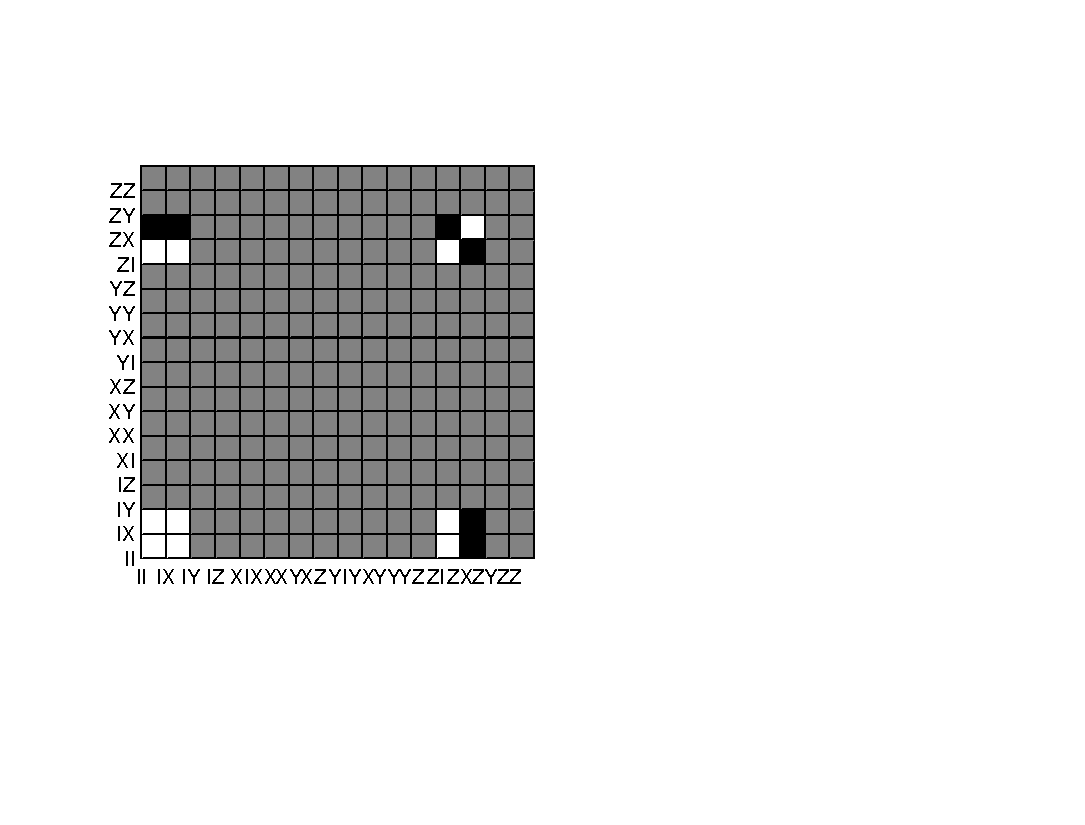
\includegraphics[width=0.35\textwidth]{CNOT_process}
\caption{Process matrix for the CNOT gate, expressed in the Pauli basis. Colour coding: grey=0, white=$1/4$, black=$-1/4$.} \label{fig:CNOT_proc_matrix}
\end{figure}

%
% Quantum Processes in Quantum Networks
%

\subsection{Quantum processes in quantum networks} \label{sec:quant_proc_in} \index{Quantum processes}

Letting $v_i$ represent the $i$th node within a route $R$, the process associated with communication from that node to the next is $\mathcal{E}_{v_i\to v_{i+1}}$. For the same network used previously, Fig.~\ref{fig:example_proc_graph} shows the quantum processes associated with the links in the network. The cumulative process associated with an entire route is therefore,
\begin{align}
\mathcal{E}_R = \mathcal{E}_{{v_{|R|-1}}\to v_{|R|}} \circ \dots \circ \mathcal{E}_{v_2\to v_3} \circ \mathcal{E}_{v_1\to v_2},
\end{align}
where $|R|$ is the number of nodes in $R$, and to simplify notation, all $v_i$ are implicitly over the route $R$.

\begin{figure}[!htb]
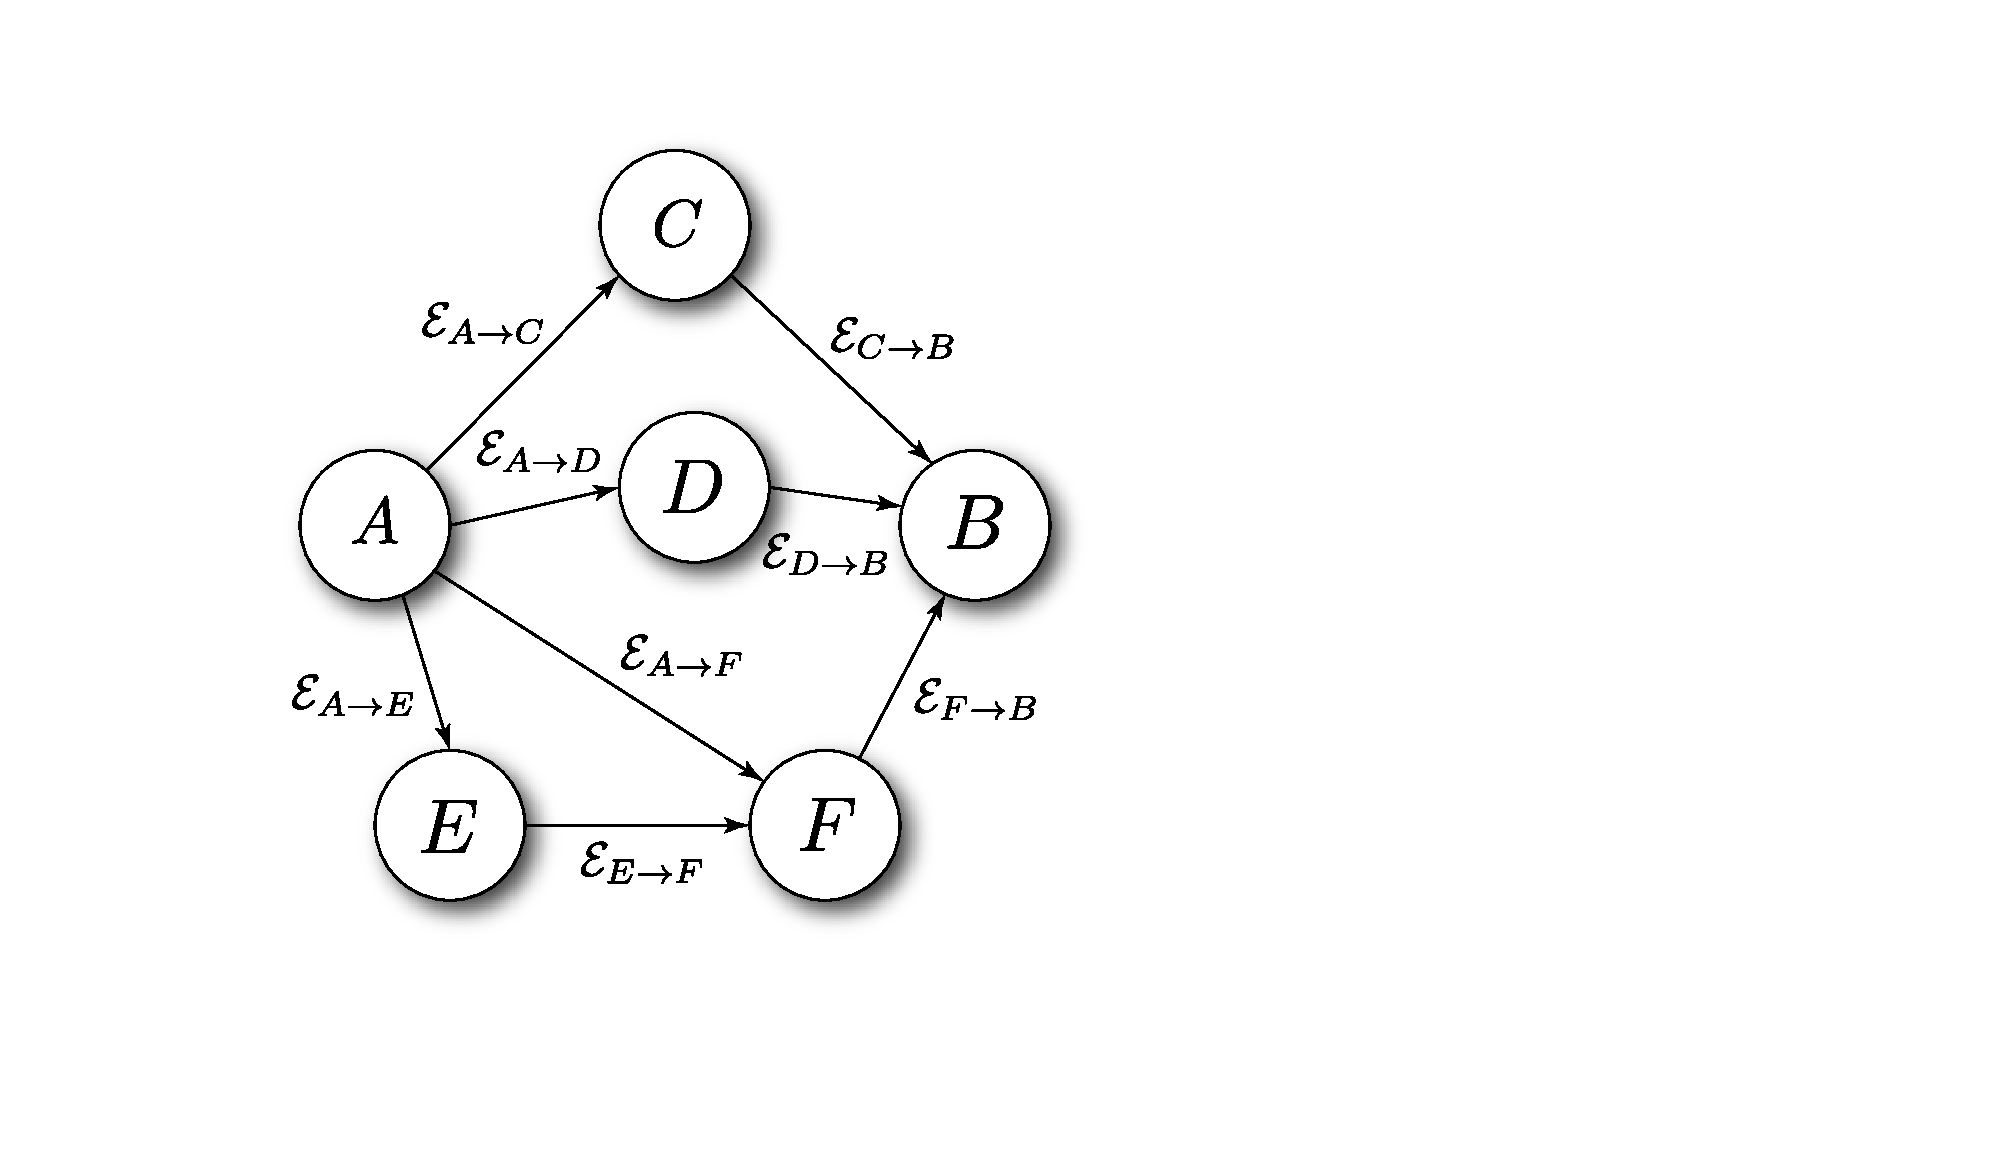
\includegraphics[width=0.3\textwidth]{example_graph}
\caption{The network from Fig.~\ref{fig:example_routes}, with the quantum processes associated with each link. The net process associated with a route is given by the composition of each of the processes over the length of the route. For example, the route \mbox{$R_1=A\to C\to B$} induces the process \mbox{$\mathcal{E}_{R_1} = \mathcal{E}_{C\to B} \circ \mathcal{E}_{A\to C}$}.} \label{fig:example_proc_graph}
\end{figure}

In general, both nodes and links in a quantum network may implement quantum processes. However, for the purposes of compatibility with the graph-theoretic algorithms described in Sec.~\ref{sec:graph_theory}, we will eliminate node processes by merging them into link processes, such that the processes in the network are described entirely by links. This reduction procedure is straightforward, shown in Fig.~\ref{fig:remove_nodes}.

\begin{figure}[!htb]
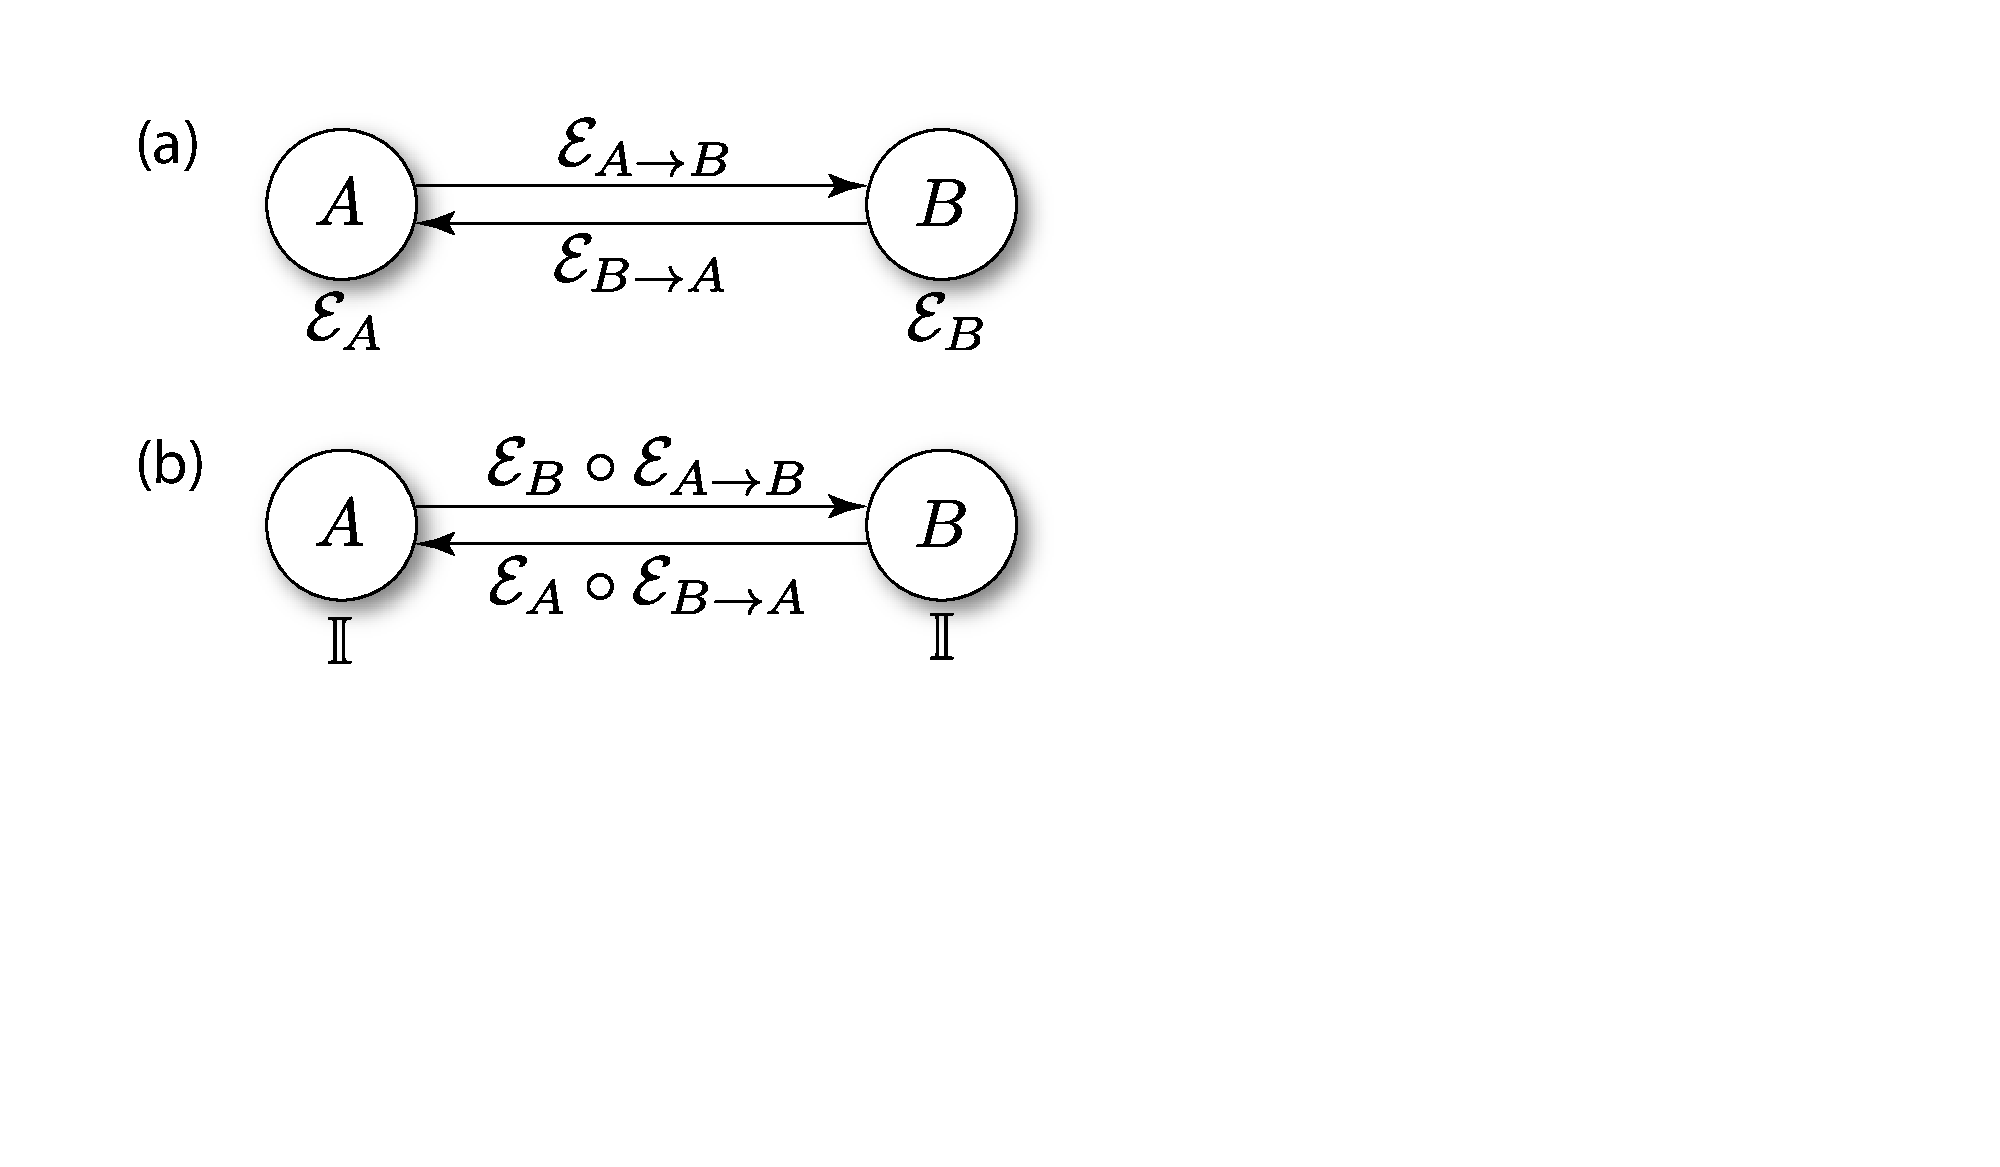
\includegraphics[width=0.35\textwidth]{remove_nodes}
\caption{Removing node processes from network graphs on a trivial network with two nodes, $A$ and $B$. Each node is associated with a quantum process ($\mathcal{E}_A$ and $\mathcal{E}_B$). Similarly, each link is associated with a process ($\mathcal{E}_{A\to B}$ and $\mathcal{E}_{B\to A}$). (a) Representation where the node and link processes are shown explicitly. (b) The node processes are replaced with identity operations by replacing each link process with the composition of the link process and its target node process. Equivalently, the cost of each node process is added to the cost of \textit{every} incoming link and then eliminated. The same may be applied for attributes rather than costs. This procedure requires that all links be directed. If undirected links are present, they may simply be replaced by two directed links, one in each direction, implementing identical quantum processes each way.} \label{fig:remove_nodes}
\end{figure}

%
% Characterising Quantum States & Channels
%

\subsection{Characterising quantum states \& channels} \label{sec:QPT}

Given a link implementing some arbitrary quantum process, it is essential that it can be experimentally determined such that network performance may be characterised. For example, if an optical channel is lossy, what is the loss rate? This is crucial when attempting to choose routing strategies that optimise certain cost metrics.

Treating a link or node as an unknown black box, \textit{quantum process tomography} (QPT) \cite{bib:ChuangNielsen97, ???} is a technique that may be applied to fully characterise the quantum process it implements, reproducing its complete process matrix. QPT has become a standard procedure, demonstrated in numerous architectures, most notably in optics \cite{bib:OBrien04, bib:RohdeGateChar05}.

QPT works in general for processes in any degree of freedom, e.g the qubit degree of freedom. However, it is important to note that full QPT requires statistics across the entire basis over which measurements are defined, which typically grows exponentially with the size of the system. For example, the number of measurement bases required to perform full QPT on $n$ qubits grows exponentially with $n$.

However, often full process characterisation is not necessary. Instead, knowing particular metrics of interest may suffice. Some of the more noteworthy such metrics will be discussed in Sec.~\ref{sec:quantum_meas_cost}. In this instance, much work has been done in the field of \textit{compressed sensing} or \textit{compressed quantum process tomography} \cite{???,compressed_sensing}, in which some process metrics of interest can be experimentally determined using far fewer physical resources (with efficient scaling!) than via a full reconstruction of the process matrix using QPT. As a most trivial example, if the loss associated with a fibre-optic channel is the metric of interest, this can be much more easily determined than by performing full QPT.

On the other hand, however, most quantum channels are designed to accommodate systems with very limited Hilbert space dimensionality per clock-cycle -- e.g a fibre-optic link might transmit just one photon at a time -- in which case there is no exponentiality to be terribly concerned about (QPT of a single-photon channel is trivial).

Importantly, it is often the case that the quantum process associated with a channel will remain constant over time. The efficiency of a length of fibre, for example, does not change. In this instance, characterising the channel need only be performed once in advance, without requiring ongoing dynamic updating. On the other hand, when communicating with satellites in low Earth orbit it is to be expected that the properties of links will be highly dynamic.

We will now explain QPT in the archetypal context of single-qubit channels, which logically generalises to multiple qubits, and can similarly be generalised to non-qubit systems also.

%
% Quantum State Tomography
%

\subsubsection{Quantum state tomography} \index{Quantum state tomography (QST)}

The first stage in QPT is \textit{quantum state tomography} (QST), where the goal is to reconstruct and unknown density matrix via measurements upon multiple copies of the state. QST is based upon the simple observation that the completeness relation\index{Completeness relation} for an arbitrary state can be expressed,
\begin{align}
\hat\rho = \sum_i \mathrm{tr}(\hat{E}_i\hat\rho)\cdot\hat{E}_i,
\end{align}
where $\{\hat{E}_i\}$ forms a complete basis for the Hilbert space of $\hat\rho$. For a single qubit this decomposition is most often performed in the Pauli basis, 
\begin{align}
\hat\rho = \mathrm{tr}(\hat\rho)\cdot\hat{\mathbb{I}} + \mathrm{tr}(\hat{X}\hat\rho)\cdot\hat{X} + \mathrm{tr}(\hat{Y}\hat\rho)\cdot\hat{Y} +\mathrm{tr}(\hat{Z}\hat\rho)\cdot\hat{Z}.
\end{align}
Of course, \mbox{$\mathrm{tr}(\hat{E}\hat\rho) = P(\hat{E}|\hat\rho)$} is just the expectation value of the measurement operator $\hat{E}$ when measuring $\hat\rho$. Thus, measuring the expectation values in each of the four Pauli bases reconstructs $\hat\rho$.

This generalises straightforwardly to multi-qubit systems, where we measure all combinations of tensor products of the Pauli operators, the number of which grows exponentially with the number of qubits $n$, as $4^n$. This introduces scalability issues for systems comprising a large number of qubits.

In the case of optical systems, entirely alternate, but equivalent, approaches may be used, such a probing the Wigner function directly using homodyne detection \cite{???}\index{Homodyne detection}.

%
% Quantum Process Tomography
%

\subsubsection{Quantum process tomography} \index{Quantum process tomography (QPT)}

Now to perform QPT we apply the unknown process to a complete basis of input states $\{\hat\rho_i\}$, and perform QST on the output state for each. This yields,
\begin{align}
\mathcal{E}(\hat\rho_j) = \sum_{i} c_{i,j} \hat\rho_i,
\end{align}
where the sum runs over the basis of states. From QST, all the coefficients $c_{i,j}$ may be determined. Next we define the following decomposition for each of the terms in the sum of Eq.~(\ref{eq:process_matrix}),
\begin{align}
\hat{E}_m \hat\rho_j \hat{E}_n^\dag = \sum_k B^{m,n}_{j,k} \hat\rho_k,
\end{align}
where $B$ defines a decomposition in the chosen basis, not dependent on any measurement results. Then we can write,
\begin{align}
\mathcal{E}(\hat\rho_j) &= \sum_{m,n} \chi_{m,n} \hat{E}_m\hat\rho_j\hat{E}_n^\dag \nonumber \\
&= \sum_{m,n} \sum_k \chi_{m,n} B^{m,n}_{j,k} \hat\rho_k.
\end{align}
Because $\hat\rho_k$ form a linearly independent basis, we can write the decomposition,
\begin{align}
c_{j,k} = \sum_{m,n} \chi_{m,n} B_{j,k}^{m,n},
\end{align}
for all \mbox{$j,k$}. From this, standard linear algebra techniques allow an inversion to obtain,
\begin{align}
\chi_{m,n} = \sum_{j,k} (B_{j,k}^{m,n})^{-1} c_{j,k},
\end{align}
thereby obtaining the full process matrix $\chi$, in the chosen basis.
\sketch{sketch_10}

\latinquote{Bulla crustulum.}

%
% Optical Encoding of Quantum Information
%

\section{Optical encoding of quantum information} \label{sec:opt_enc_of_qi} \index{Optical encoding of quantum information}

While all-optical quantum computing is an unlikely architecture for future scalable quantum computers, it is all but inevitable that optics will play a central role in quantum communications networks. Foremost, this is because photons are `flying' by their very nature and can very easily be transmitted across large distances -- it's quite challenging to transmit a superconducting circuit containing information from Australia to Mozambique in the blink of an eye! Additionally, optical states are, in many cases, relatively easy to prepare, manipulate and measure, and can also be readily interfaced with other physical quantum systems (Sec.~\ref{sec:opt_inter}), allowing the transfer of quantum information from optical communications systems to some other architecture better suited to a given task.

Optical systems are very versatile, allowing quantum information to be optically encoded in a number of ways -- into single photons, many photons, or even an indeterminate number of photons, and in both discrete or continuous degrees of freedom. Different types of encodings may have very different properties in terms of the errors they are susceptible to (Sec.~\ref{sec:errors_in_nets}).

When dealing with single photons, information can be encoded in a number of ways. Most obviously, it can be encoded into the polarisation basis, allowing one qubit of information per photon (i.e horizontal and vertical polarisation represent the logical $\ket{0}$ and $\ket{1}$ states). Or it could be directly encoded into the photon-number basis. However, other degrees of freedom, such as the spectral/temporal degrees of freedom could be employed, encoding information into time- or frequency-bins, with potentially far more levels than a simple polarisation qubit \cite{bib:RohdeInfCap13}. Next we discuss the main methods for optical encoding of quantum information.

%
% Single Photons
%

\subsection{Single photons} \label{sec:single_phot_enc} \index{Single-photon encoding}

A very attractive feature of single photons is that they undergo very little decoherence, even over large distances -- dephasing (Sec.~\ref{sec:dephasing_error}) in the polarisation degree of freedom, for example, is negligible in free-space. They are, however, very susceptible to loss, and protocols relying on many single-photon states suffer exponential decay in their success rates as the number of photons is increased (Sec.~\ref{sec:eff_err}).

We can encode a single qubit into a single photon in the polarisation basis using the horizontal and vertical polarisation degrees of freedom. Equivalently, one can employ `dual rail' encoding, whereby a single photon is placed into a superposition across two spatial modes. Finally, one can use time-bin encoding, whereby discrete windows of time represent logical basis states when occupied by a photon. This leads to the equivalent representations for logical qubits ($L$),
\begin{align} \label{eq:single_photon_enc}\index{Polarisation encoding} \index{Dual-rail encoding}
\ket{\psi}_\text{qubit} &\equiv \alpha\ket{0}_L + \beta\ket{1}_L, \nonumber \\
\ket{\psi}_\text{pol} &\equiv \alpha\ket{H} + \beta\ket{V}, \nonumber \\
\ket{\psi}_\text{dual} &\equiv \alpha\ket{0,1} + \beta\ket{1,0}, \nonumber \\
\ket{\psi}_\text{temporal} &\equiv \alpha\ket{0_t,1_{t+\tau}} + \beta\ket{1_t,0_{t+\tau}}.
\end{align}
Conversion between polarisation and dual-rail encoding is straightforward and deterministic using standard optical components, as described in Fig.~\ref{fig:pol_to_dual_conv}.

\begin{figure}[!htb]
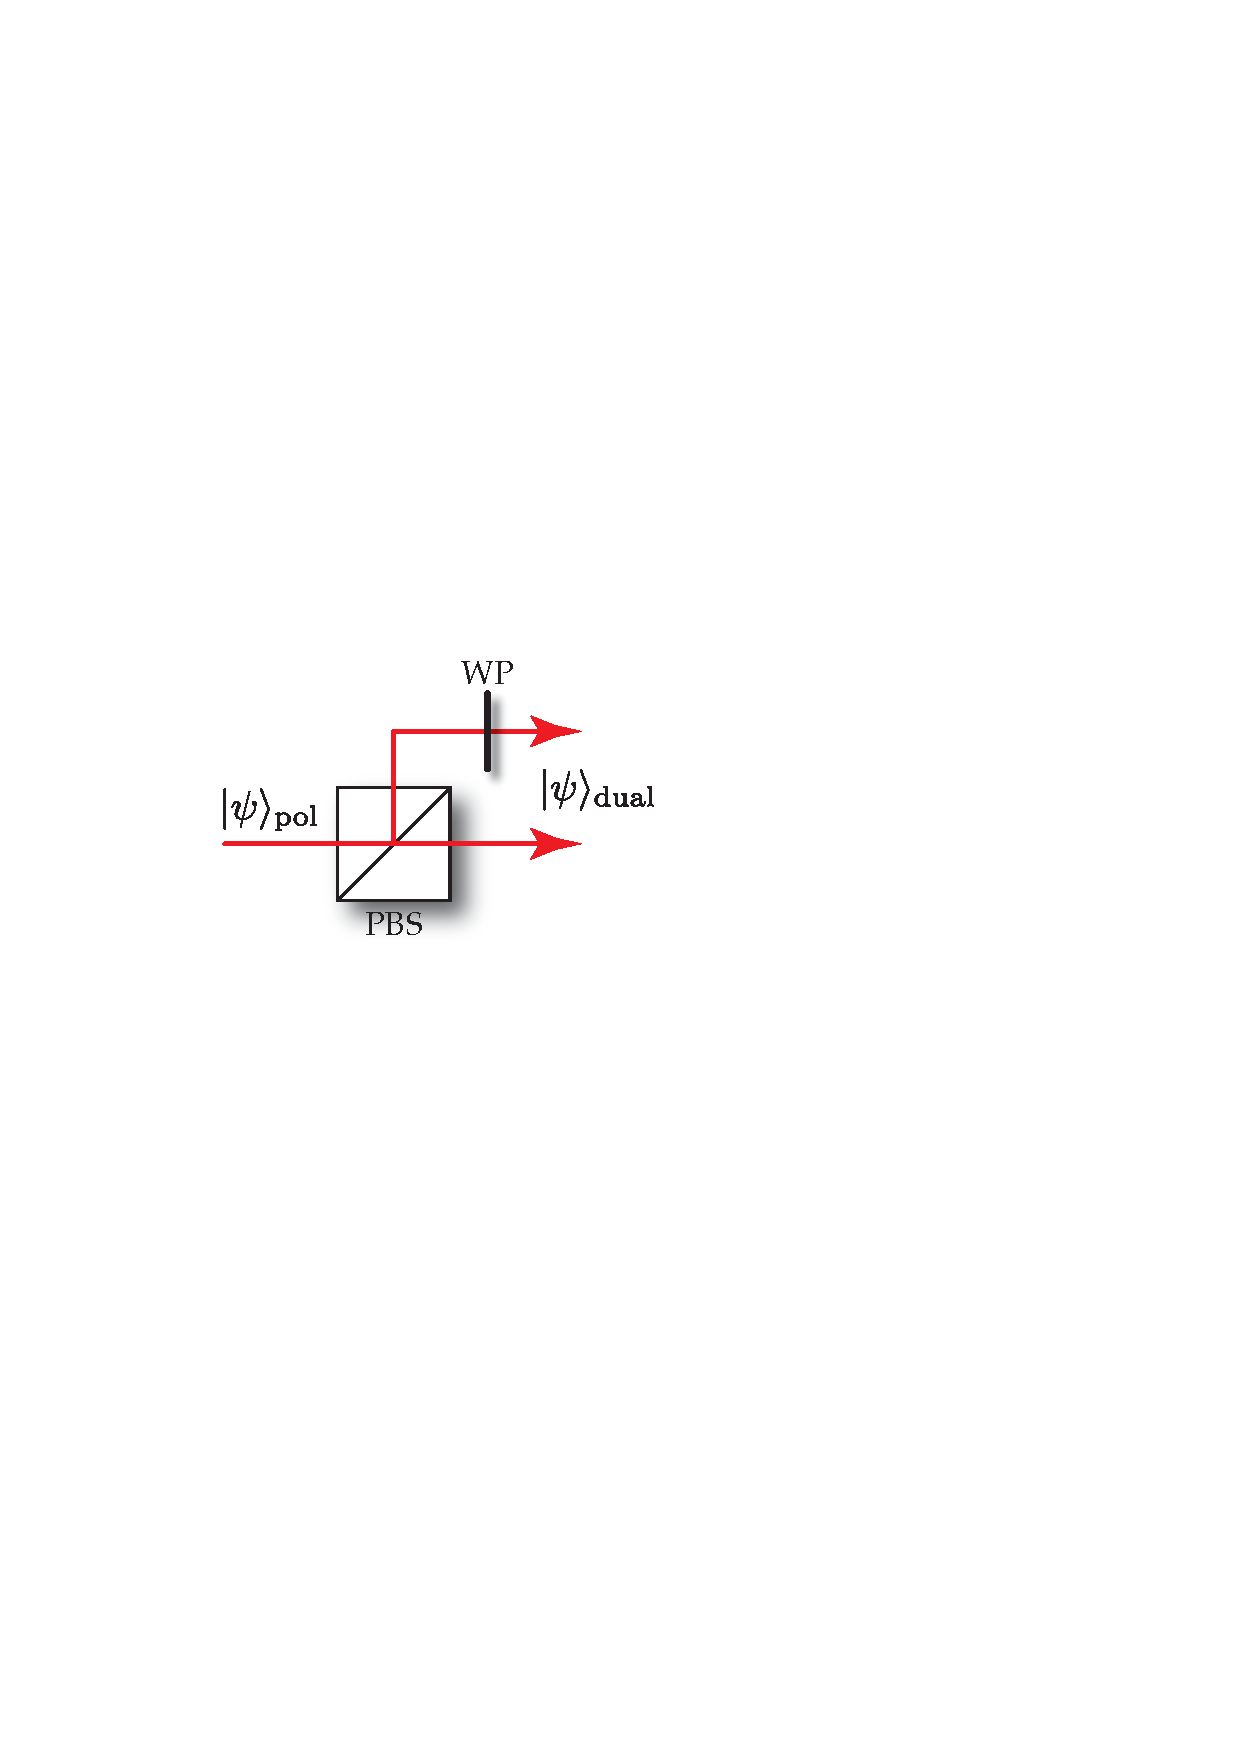
\includegraphics[width=0.3\textwidth]{pol_to_dual_conversion}
\caption{Conversion from single-photon polarisation encoding to dual-rail encoding, using a polarising beamsplitter (PBS) and wave-plate (WP). The PBS separates the polarisation components into two distinct spatial modes. The WP then rotates the polarisation of one of the spatial modes such that it has the same polarisation as the other. Conversion from dual-rail to polarisation encoding is just the reverse of this procedure.} \label{fig:pol_to_dual_conv}\index{Polarising beamsplitters}
\end{figure}

Note that polarisation encoding requires a single spatial mode per qubit, whereas dual-rail encoding requires two. Polarisation encoding brings with it the advantage that arbitrary single-qubit operations may be implemented using wave-plates, which maintain coherence between the basis states extraordinarily well. In dual-rail encoding, on the other hand, single-qubit operations are implemented using beamsplitter operations between the two spatial modes, which must be interferometrically stable, since consecutive single-qubit operations yields Mach-Zehnder (MZ) interference \cite{bib:Zehnder1, bib:Zehnder2}\index{Mach-Zehnder (MZ) interference}, to be discussed in detail in Sec.~\ref{sec:MZ_inter}.

Single-photon encodings are extremely important, as they form the basis for universal linear optics quantum computing (Sec.~\ref{sec:KLM_univ}), \textsc{BosonSampling} (Sec.~\ref{sec:BS}) and quantum walks (Sec.~\ref{sec:QW}). They are also the simplest optical states for representing single qubits.

%
% Photon-number
%

\subsection{Photon-number} \index{Photon-number encoding}

Of course, the photon-number degree of freedom needn't be limited to 0 or 1 photons. By fully exploiting the photon-number degree of freedom, we can encode a qudit\footnote{A $d$-level system, as opposed to a qubit's two levels.}\index{Qudits} of arbitrary dimension into a single optical mode,
\begin{align} \label{eq:number_qudit}
\ket\psi_\text{qudit} \equiv \sum_{n=0}^\infty \alpha_n \ket{n}.
\end{align}
This may give the impression that a single optical mode has infinite information capacity. Needless to say, this sounds too good to be true, and it is. Loss decoheres photon-number-encoded states exponentially with photon-number, since for large photon-number the probability of a number state retaining its photon-number exponentially asymptotes to zero. So although in principle we can encode an $\infty$-level qudit, the moment any non-zero loss is introduced, this exponential dependence destroys the state (Sec.~\ref{sec:eff_err}).

While photon-number encoding can be useful for communications purposes, it is not very practical for quantum information processing tasks, since operations between basis states are not energy preserving, with each basis state having energy \mbox{$E=n\hbar\omega$}, where $\omega$ is frequency, and $\hbar$ is Planck's constant. Thus, qudit operations would need to be active processes.

%
% Spatio-Temporal Qudit Encoding
%

\subsection{Spatio-temporal} \label{sec:spatio_temporal} \index{Spatio-temporal encoding}

Completely independent of the photon-number degree of freedom, are the spatio-temporal degrees of freedom, which encode the spatial, temporal, and spectral/temporal structure of photons. In the temporal domain, for example, we could define the temporal structure of a single photon as,
\begin{align}
\ket\psi_\text{temporal} = \int_{-\infty}^\infty \psi(t) \hat{a}^\dag(t)\,dt\,\ket{0},
\end{align}
where $\hat{a}^\dag(t)$ is the time-specific photonic creation operator, and $\psi(t)$ is the temporal distribution function \cite{bib:RohdeFreqTemp05}.

Alternately, we can define \textit{mode operators} \cite{bib:RohdeMauererSilberhorn07}\index{Mode operators}, which are mathematically equivalent to creation operators, but create photons with a specific temporal envelope,
\begin{align}
\hat{A}^\dag_\psi &= \int_{-\infty}^\infty \psi(t) \hat{a}^\dag(t)\,dt, \nonumber \\
\ket\psi_\text{temporal} &= \hat{A}^\dag_\psi \ket{0}.
\end{align}
Mode operators commute, inheriting this property directly from photonic creation operators,
\begin{align}
\left[\hat{A}^\dag_{\psi_1},\hat{A}^\dag_{\psi_2}\right]=0.
\end{align}

Now by defining an orthonormal basis of temporal distribution functions, $\{\xi_i\}$, such that,
\begin{align} \label{eq:spec_orth_def}
\bra{0} \hat{A}_{\xi_i} \hat{A}^\dag_{\xi_j}\ket{0} = \delta_{i,j},
\end{align}
we can encode a qudit of arbitrary dimension into the spatio-temporal degrees of freedom,
\begin{align}
\ket\psi_\text{qudit} \equiv \sum_{i=0}^\infty \alpha_i \hat{A}^\dag_{\xi_i} \ket{0}.
\end{align}

This encoding allows a qudit of arbitrary dimension to be encoded into a single spatial mode. Again, however, summing to infinity is somewhat fanciful, given any physically realistic spatio-temporal error model, such as an imperfect frequency response in the channel, e.g a bandpass response of an optical fibre or photo-detector.

%
% Time-Bins
%

\subsection{Time-bins} \label{sec:time_bin} \index{Time-bin encoding}

In time-bin encoding we define our basis of modes (whether it be qubits or higher-dimensional qudits\index{Qudits}) as distinct, non-overlapping time-bins, which are localised wave-packets in the temporal degree of freedom, each separated from the next by some fixed interval $\tau$. This can be considered a special case of spatio-temporal encoding\index{Spatio-temporal encoding}, where the basis mode functions satisfy the relation,
\begin{align}
\xi_{j}(t) = \xi_0(t-j\tau),
\end{align}
as well as the usual orthonormality constraints. Here $\tau$ is sufficiently large, and $\xi_i(t)$ sufficiently temporally localised, that the temporal modes are orthogonal as per Eq.~(\ref{eq:spec_orth_def}).

Time-bin encoding arises naturally in architectures where the photon source driving the system is operating at a high repetition rate\index{Repetition rate}, $R$, in which case \mbox{$\tau=1/R$}. Architectures for optical quantum computing have been described \cite{bib:RohdeLoop15, bib:RohdeUnivLoop15}, and experimentally demonstrated \cite{???}, based entirely on time-bin encoding.

These schemes can be very resource efficient, since a single source operating at high repetition rate can replace an entire bank of distinct sources that would ordinarily be required in spatial architectures. Similarly, a single time-resolved detector, with resolution at least $\tau$, can replace a bank of detectors operating in parallel. And only a single spatial mode is required to store an arbitrary number of qubits/qudits, so long as it is long enough to support the entire pulse-train -- at least $2n\tau$ for $n$ qubits.

In the schemes of \cite{bib:RohdeLoop15, bib:RohdeUnivLoop15}, entire optical quantum computing protocols can be efficiently constructed using only a single source, a single detector, two delay-lines, and three dynamically-controlled beamsplitters, irrespective of the size of the computation, an enormous resource saving compared to traditional spatial encodings. Furthermore, in these schemes, there is only a single point of interference, greatly simplifying optical interferometric alignment, which would ordinarily require simultaneously aligning a large number of optical elements, as many as $O(m^2)$ elements for an $m$-mode network \cite{bib:Reck94}.

%
% Coherent States
%

\subsection{Coherent states} \label{sec:coherent_state_enc} \index{Coherent state encoding}

When encoding information optically, we needn't restrict ourselves to photon-number states. We also have a lot of flexibility to encode information in phase-space using continuous variable (CV) states, where phase and amplitude relations encode quantum information \cite{bib:CahillGlauber69}.

As a simple example, consider coherent states. These are particularly useful since they are pure states, with well defined coherence relationships, and are closely approximated by laser sources, and therefore readily available in the lab.

A coherent state, $\ket\alpha$, is parameterised by a single complex parameter, $\alpha$, given by a phase and amplitude,
\begin{align}\index{Coherent states}
\ket{\alpha} = e^{-\frac{|\alpha|^2}{2}} \sum_{n=0}^\infty \frac{\alpha^n}{\sqrt{n!}} \ket{n}.
\end{align}
By manipulating these parameters, information can be encoded into coherent states. We could, for example, define two coherent states of opposite phase to represent qubit basis states,
\begin{align}
\ket{0} &\equiv \ket{\alpha}, \nonumber \\
\ket{1} &\equiv \ket{-\alpha}.
\end{align}
Note, however, that this representation for qubits is only approximate, since the two basis states are not perfectly orthogonal,
\begin{align}
\langle -\alpha|\alpha \rangle = e^{-2|\alpha|^2},
\end{align}
which is non-zero for any finite $\alpha$, whereas for ideal qubits we require \mbox{$\langle 0|1\rangle = 0$}. However, for large $\alpha$, $\ket{\pm\alpha}$ closely approximate orthogonality.

This representation for qubits using coherent states is easily generalised to qudits by considering coherent states orbiting the origin of phase-space at equal angular intervals of \mbox{$2\pi/d$}, for a $d$-level qudit. The $k$th qudit basis state is then,
\begin{align}
\ket{k}_d = \ket{e^{ik/d}\alpha},
\end{align}
for \mbox{$k=0,\dots,d-1$}, where again the basis states are non-orthogonal, but closely approximate orthogonality for large $\alpha$.

Note that despite being pure states, with well-defined coherence, coherent states are considered classical, as they are unable to encode quantum information. That is, the coherence relationships cannot be exploited for the encoding of qubits or qudits.

Coherent states are useful in that they are easy to prepare using modern lasers, including laser diodes, and by turning up the amplitude can be transmitted over long distances, with loss not affecting quantum coherence, only the amplitude (Sec.~\ref{sec:eff_err}).

%
% Cat States
%

\subsection{Cat states} \label{sec:cat_enc} \index{Cat state encoding}\index{Cat states}

Another type of CV state, which can in fact encode quantum information, is superpositions of coherent states (colloquially known as `cat' states), with the encoding \cite{???},
\begin{align}
\ket{0} &\equiv \frac{1}{\sqrt{2(1+e^{-2|\alpha|^2})}} (\ket{\alpha}+\ket{-\alpha}) \nonumber \\
&= \ket{\text{cat}_+(\alpha)},\nonumber \\
\ket{1} &\equiv \frac{1}{\sqrt{2(1-e^{-2|\alpha|^2})}}(\ket{\alpha}-\ket{-\alpha}) \nonumber \\
&= \ket{\text{cat}_-(\alpha)}.
\end{align}
These two basis states contain strictly even or odd photon-number terms respectively (i.e they have well-defined parity), implying that, unlike coherent states, they are always orthogonal, regardless of amplitude,
\begin{align}
\langle\text{cat}_+(\alpha)|\text{cat}_-(\alpha)\rangle = 0 \,\,\forall\,\alpha,
\end{align}
making them directly appropriate for qubit encoding, even for weak coherent amplitudes.

Unfortunately, cat states are notoriously difficult to prepare, and extremely sensitive to loss (Sec.~\ref{sec:single_phot_enc}) and dephasing (Sec.~\ref{sec:dephasing_error}). This arises because loss of a single photon flips the parity of the state to an orthogonal one, meaning that as $\alpha$ increases, the state is exponentially more susceptible to decohering into a mixture of the logical basis states.

However, modulo these difficulties, with a resource of cat states at one's disposal, universal quantum computation may be realised using post-selected linear optics \cite{bib:JeongRalph05, bib:Gilchrist04}.

%
% Thermal State Encoding
%

\subsection{Thermal states} \index{Thermal state encoding}\label{sec:thermal_states}

In some quantum protocols, although the inner workings may be quantum mechanical in nature, the inputs and outputs needn't capture any quantum coherence -- sometimes \textit{classical} information is sufficient for communications. As discussed above, coherent states are the archetypal example of this, and this is in fact the norm in present-day classical fibre-optic communication, where coherent states prepared from laser diodes are employed.

Another, and even simpler option, is thermal states. These are obtained by fully dephasing a coherent state, retaining the amplitudes, while nullifying all the coherence terms,
\begin{align}
\hat\rho_\text{thermal}(\alpha) = e^{-|\alpha|^2} \sum_{n=0}^\infty \frac{|\alpha|^2}{n!}\ket{n}\bra{n}.
\end{align}

Thermal states can encode classical information into their amplitudes, polarisations, or time-bins, as before. The advantage of this type of encoding is that thermal states are trivial to prepare and measure (a normal incandescent lightbulb produces thermal states of light). However, they are purely classical states, do not undergo interference with one another, and are therefore useless for, for example, entangling qubits via which-path erasure, any other type of coherent interferometric process, or for representing quantum information such as qubits.

%
% Phase-Space
%

\subsection{Phase-space} \label{sec:exotic} \index{Phase-space encoding}

The optical encodings presented thus far are the main textbook examples. However, many other encodings, particularly in phase-space, can also be used to encode both quantum or classical information and perform quantum computations upon them. The aforementioned coherent states and cat states are classic examples of states well-suited to a phase-space representation. But this extends to many other states, such as Gaussian states more generally.

In phase-space, the most common representations of optical states are in terms of quasi-probability functions\index{Quasi-probability functions}\footnote{The term `quasi-probablity' arises because in some regimes (for example, strictly non-negative $P$-functions), the function has a true probabilistic interpretation. However this interpretation breaks down for any negativity in the $P(\alpha)$, since negative probabilities have no meaningful classical interpretation.}:
\begin{itemize}\index{$P$-function}\index{$Q$-function}\index{Wigner function}
\item $P$-function: represents a state as a quasi-mixture of coherent states. When the $P$-function is strictly non-negative, it can be interpreted as a perfect classical mixture of coherent states. However, with any negativity this classical interpretation breaks down, hence `quasi'-probability. In general, the $P$-function representation for a state is not unique.
\begin{align}
\hat\rho = \int\!\!\!\int P(\alpha) \ket{\alpha}\bra{\alpha} d^2\alpha.
\end{align}
\item $Q$-function: represents a state in terms of its overlap with the complete set of all coherent states, which form an over-complete basis.
\begin{align}
Q(\alpha) = \frac{1}{\pi} \bra{\alpha}\hat\rho\ket{\alpha}.
\end{align}
\item Wigner function: also has a quasi-probability interpretation, and negativity is qualitatively associated with `quantumness'. The Wigner function of a state is unique, and isomorphic to the density operator, making it perhaps the most useful phase-space representation for quantum states of light.
\begin{align}
W(x,p) = \int e^{ips/\hbar} \left\langle{x-\frac{s}{2}}\right| \hat\rho \left|{x+\frac{s}{2}}\right\rangle ds.
\end{align}
\end{itemize}
These representations, whilst entirely equivalent to a photon-number basis representation, are far easier to work with for many types of states. Most notably, Gaussian states are conveniently represented and manipulated using phase-space representations.

\comment{Squeezed states - refer back to CV section}

%
% Non-Optical Encoding
%

\subsection{Non-optical encoding}\index{Non-optical encodings}

In a non-optical context, the elementary unit of quantum information -- the qubit -- can be naturally encoded into any system with a natural or engineered two-level structure. This actually encompasses a broad range of possibilities, including, amongst many others:
\begin{itemize}
\item \index{2-level systems}Two-level atoms: let two distinct electron energy levels, with long lifetimes, represent the two logical basis states.
\item \index{$\lambda$-configuration systems}$\lambda$-configuration atoms: atoms with two degenerate ground states, which encode the logical qubit, and an additional excited state, which may be transitioned to upon excitation from only one of the ground states. Relaxation from the excited state enables optical coupling via the emitted photon.
\item \index{Quantum dots}Quantum dots: are essentially artificial atoms, which can be engineered with custom band-structures, allowing two- or higher-level qudits to be easily fabricated.
\item \index{Nitrogen-vacancy (NV) centres}Nitrogen-vacancy (NV) centres: are a type of point defect in diamond, which has a very well defined energy level structure that may be utilised to represent qubits.
\item \index{Atomic ensembles}Atomic ensembles: encode quantum information similarly to a single atom, except that the excitation is a \textit{collective} one, in superposition across all the atoms in the ensemble.
\item \index{Superconducting rings}Superconducting rings: a superposition of current flow direction in a superconducting ring represents the two logical basis states.
\item \index{Trapped ions}Trapped ions: qubits are encoded into stable electronic states of electromagnetically trapped ions.
\end{itemize}

Clearly the non-optical elements in a quantum network must somehow interface with optical states, such that communication is facilitated. This is discussed later in Sec.~\ref{sec:opt_inter}.
\sketch{sketch_11}

\latinquote{Audaces fortuna juvat.}

%
% Errors in Quantum Networks
%

\section{Errors in quantum networks} \label{sec:errors_in_nets} \index{Errors in quantum networks}

As with classical data, quantum data is susceptible to corruption during transmission. However, in addition to all the usual classical error models, quantum information is subject to further uniquely quantum errors. These errors can be represented using the quantum process formalism and fully characterised using QPT (Sec.~\ref{sec:QPT}). We now briefly discuss several of the dominant errors arising in quantum systems, paying especial attention to error models acting on qubits and optical states, as these are the most relevant in a quantum networking context.

%
% Known Unitaries
%

\subsection{Known unitaries} \index{Unitary errors}

The most trivial error mechanism is when a (potentially multi-qubit) unitary channel (e.g an identity channel for the purposes of quantum memory) actually implements some unitary transformation, $\hat{U}$, that is not that which is desired. However, the unitary is constant, not varying from trial to trial, and is known, which can be easily determined by performing QPT on the channel. For example, an optical fibre might induce a polarisation rotation on transmitted photons, but the fibre isn't changing and neither is the rotation. If consistently implementing the same known unitary then reversing it is straightforward in most architectures, by applying $\hat{U}^\dag$, since $\hat{U}^\dag\hat{U}=\hat{\mathbb{I}}$.

%
% Unknown Unitaries
%

\subsection{Unknown imperfect unitaries} \index{Unitary errors}

Alternate to known unitaries, the unitary operation implemented by a node/channel may deviate from that which is desired, in an unknown manner, thereby implementing a slightly different operation than that which we intended to engineer. Specifically, the effective unitary can be represented as the ideal unitary, augmented by some deviation matrix,
\begin{align}
	\hat{U}_\text{effective} = \hat{U}_\text{ideal} + \hat{\Delta}_\text{error},
\end{align}
where the matrix elements of $\hat{\Delta}_\text{error}$ are unknown, but hopefully small. Since the unknown deviation matrix needn't be constant, it will be a function of random variables, evaluated independently for each trial of the process. Furthermore, since the deviation matrix may vary from trial to trial, QPT cannot be employed to characterise it, unlike unitaries with fixed errors.

%
% Loss
%

\subsection{Loss} \label{sec:eff_err} \index{Loss channel}

Given that quantum communication links will typically be optical, the dominant error mechanism is likely to be loss. We let the efficiency, $\eta$, of an optical quantum process be the probability that a given photon entering the channel leaves the channel in the desired mode, or probability \mbox{$1-\eta$} of being lost. In the case of information encoded into single-photon states, e.g using the polarisation degree of freedom, $\eta$ corresponds exactly to the success probability of the communication.

When implementing protocols employing post-selection upon detecting all photons, the protocol will be non-deterministic, where loss dictates the protocol's success probability. Specifically, with $n$ photons, each with efficiency $\eta$, the net post-selection success probability of the entire device is $\eta^n$. This implies an exponential number of trials, \mbox{$(1/\eta)^n$}, is required in post-selected protocols. Clearly this exponential scaling is of concern, requiring demanding efficiencies in future large-scale implementations.

Formally, let $\mathcal{E}^\text{loss}_\eta$ be the loss channel with efficiency $\eta$. The channel acting on an initially pure single-photon state, $\ket{1}$, can be modelled as a beamsplitter with transmissivity $\eta$ acting on the state, where the reflected mode is traced out, shown in Fig.\ref{fig:loss_model}. This yields the quantum process,
\begin{align}
\mathcal{E}^\text{loss}_\eta(\hat\rho) = \text{tr}_B[\hat{U}_\text{BS}(\hat\rho_A\otimes\ket{0}_B\bra{0}_B)\hat{U}_\text{BS}^\dag],
\end{align}
where $\hat{U}_\text{BS}$ is the beamsplitter operation. In the special case of the vacuum and single-photon states, which is most relevant to qubit encodings, we obtain,
\begin{align}
	\mathcal{E}^\text{loss}_\eta(\ket{0}\bra{0}) &= \ket{0}\bra{0}, \nonumber \\
\mathcal{E}^\text{loss}_\eta(\ket{1}\bra{1}) &= (1-\eta)\ket{0}\bra{0} + \eta\ket{1}\bra{1}.
\end{align}
This dynamic is of the same form as amplitude damping (Sec.~\ref{sec:amp_damp}). In the general case of an $n$-photon Fock state, we obtain,
\begin{align}
	\mathcal{E}^\text{loss}_\eta(\ket{n}\bra{n}) = \sum_{i=0}^n \binom{n}{i} \eta^i(1-\eta)^{n-i} \ket{i}\bra{i}.
\end{align}

\begin{figure}[!htb]
	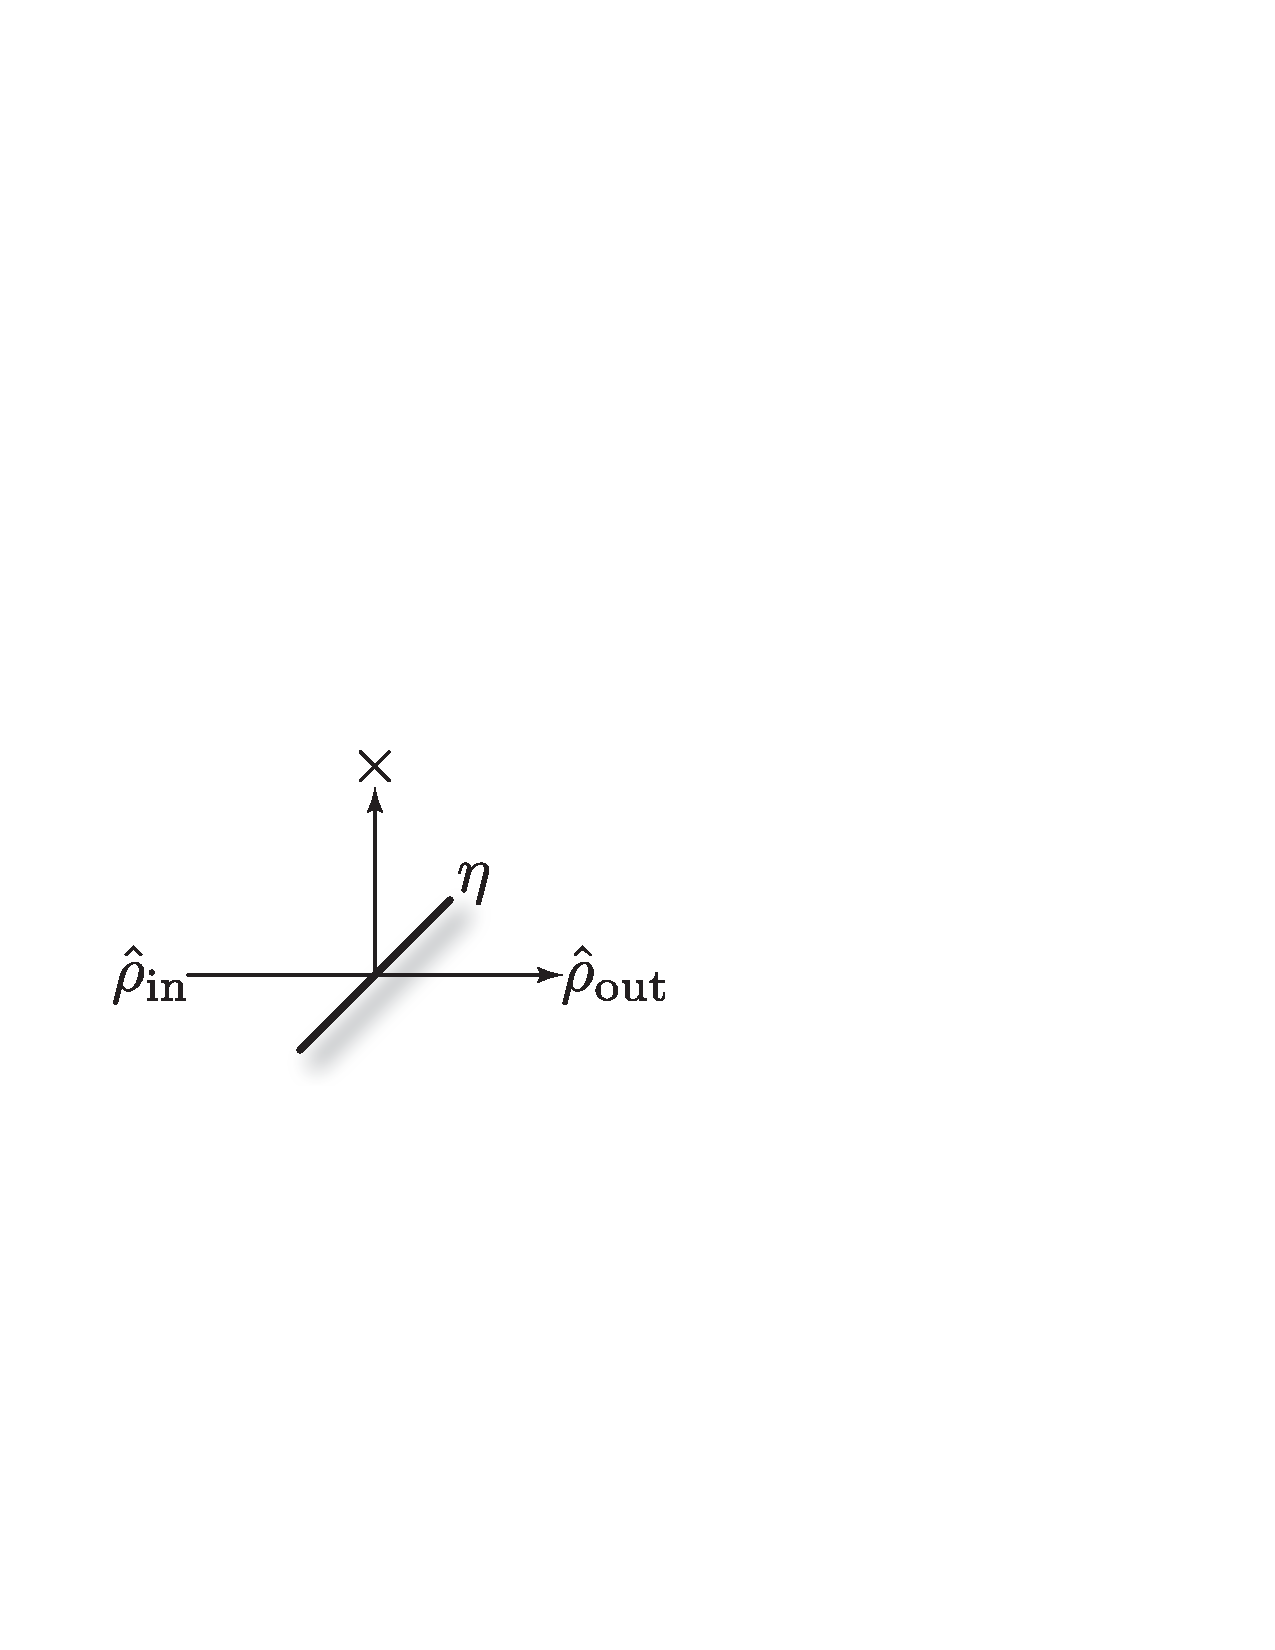
\includegraphics[width=0.25\textwidth]{loss_model}
	\caption{Model for the loss channel. The input state, $\hat\rho_\text{in}$, passes through a beamsplitter of transmissivity $\eta$, and the reflected mode discarded, yielding the lossy output state \mbox{$\hat\rho_\text{out} = \mathcal{E}^\text{loss}_\eta(\hat\rho_\text{in})$}.} \label{fig:loss_model} \index{Loss channel}
\end{figure}

Consecutive loss channels act multiplicatively,
\begin{align}
\mathcal{E}_{\eta_1}^\text{loss} \circ \mathcal{E}_{\eta_2}^\text{loss} = \mathcal{E}_{\eta_1 \eta_2}^\text{loss}.
\end{align}
In the special case of linear optics circuits, loss channels have the elegant property that, provided the loss rate is uniform across all modes, they can be commuted through the circuit to the front or back \cite{???}\index{Loss commutation}. Specifically,
\begin{align}
(\mathcal{E}_{\eta}^\text{loss})^{\otimes m} \circ \mathcal{E}_U = \mathcal{E}_U \circ (\mathcal{E}_{\eta}^\text{loss})^{\otimes m},
\end{align}
where $\mathcal{E}_U$ is a unitary linear optics process, implementing a photon-number-preserving map of the form of Eq.~(\ref{eq:LO_unitary_map}). This simplifies the treatment of distinct system inefficiencies (such as source, network and detector inefficiencies) by allowing us to commute them to the beginning or end of the circuit and combine them together into a single net efficiency. In many scenarios, this allows the different system inefficiencies to be dealt with via post-selection.

This process would apply equivalently to both horizontal and vertical polarisations. Therefore, via linearity, the loss channel acting on a polarisation-encoded qubit (Sec.~\ref{sec:single_phot_enc}) yields,
\begin{align}
\mathcal{E}^\text{loss}_\eta(\ket\psi_\text{pol}\bra\psi_\text{pol}) = (1-\eta) \ket{0}\bra{0} + \eta\ket\psi_\text{pol}\bra\psi_\text{pol}.
\end{align}
The same applies in the context of dual-rail encoding. Note that while this transformation mixes the state in the photon-number degree of freedom, it preserves coherence between the horizontal and vertical single-photon components. Thus, upon successful post-selection, the state is projected back onto the desired qubit state.

In the case of higher order photon-number encoding of qudits\index{Qudits}, as per Eq.~(\ref{eq:number_qudit}), the probability of an $n$-photon basis state being maintained scales as $\eta^n$. That is, if the highest photon-number term in our qudit is $n$, that component has an exponentially low probability of being preserved through the loss channel. For this fundamental reason, photon-number encoding does not enable infinite-dimensional qudits to be encoded.

Coherent states are the one example of states, which are in a sense robust against loss, since a lossy coherent state is another coherent state with lower amplitude, but without any loss in coherence,
\begin{align}
\mathcal{E}^\text{loss}_\eta(\ket\alpha\bra\alpha) = \ket{\eta\alpha}\bra{\eta\alpha}.
\end{align}
This arises because coherent states are eigenstates of the photonic annihilation operator, \mbox{$\hat{a}\ket{\alpha}=\alpha\ket{\alpha}$}.

However, although coherence is maintained under the loss channel, the process is irreversible, since noise-free amplitude amplification is not possible in general \cite{???}. Thermal states exhibit the same property, that a loss channel simply yields another thermal state with reduced amplitude, although these exhibit no coherence.

To the contrary, while cat states (Sec.~\ref{sec:cat_enc}) are simple superpositions of coherent states, they are extremely sensitive to loss. This is because cat states have well-defined photon-number parity (strictly even or odd photon-number), and therefore the loss of just a single photon will flip a cat state to an orthogonal one. Since the probability of photon loss occurring increases exponentially with photon-number, large amplitude cat states are exponentially sensitive to loss channels.

Similarly, NOON states (Sec.~\ref{sec:NOON}) undergo complete wave-function collapse if just a single photon is lost to the environment, and because there are $N$ photons in total, the probability of wave-function collapse grows exponentially with photon-number.

%
% Dephasing
%

\subsection{Dephasing} \label{sec:dephasing_error} \index{Dephasing channel}

The dephasing error model describes the deterioration of quantum coherence in a state. It does not change the actual amplitudes of the components in the superposition, but rather reduces the state to a mixture of those components. Thus, dephasing can be thought of as destroying quantum information (coherence), while retaining classical information (probability amplitudes). In terms of qubits, dephasing is most commonly represented using the Kraus representation,
\begin{align} \label{eq:dephasing_channel}
\mathcal{E}_p^\text{dephasing}(\hat\rho) = p\cdot\hat\rho + (1-p)\cdot \hat{Z}\hat\rho\hat{Z},
\end{align}
where $\hat\rho$ is the state of a single qubit, and $\hat{Z}$ is the Pauli phase-flip operator\footnote{Bit-flip\index{Bit-flip channel} and bit-phase-flip\index{Bit-phase-flip channel} channels may be represented similarly by replacing $\hat{Z}$ with $\hat{X}$ or $\hat{Y}$ respectively, although these don't arise as naturally as dephasing in many physical contexts.}. Intuitively this tells us that the dephasing channel creates a mixture of an input state with its phase-flipped self.

An alternate interpretation for the dephasing channel is that it is equivalent to the outside environment measuring $\hat\rho$ in the logical ($\hat{Z}$) basis, but unknown to us, thereby projecting the state onto one basis state or another, yielding a mixture of the two.

Dephasing acting on $\hat\rho$ can be very elegantly visualised as simply nullifying the off-diagonal matrix elements, i.e eliminating coherence terms. Dephasing is a ubiquitous error mechanism and affects all current quantum computing architectures.

Consecutive dephasing channels act multiplicatively as,
\begin{align} \label{eq:multi_deph}
\mathcal{E}_{p_1}^\text{dephasing} \circ \mathcal{E}_{p_2}^\text{dephasing} = \mathcal{E}_{p_1 p_2}^\text{dephasing}.
\end{align}

As a simple example, consider the \mbox{$p=1/2$} dephasing channel acting on the \mbox{$\ket{+} = \frac{1}{\sqrt{2}}(\ket{0}+\ket{1})$} state. Then we have,
\begin{align}
\mathcal{E}^\text{dephasing}_{1/2}(\ket{+}\bra{+}) &= \frac{1}{2} (\ket{+}\bra{+} + \hat{Z}\ket{+}\bra{+}\hat{Z}) \nonumber \\
&= \frac{1}{2} (\ket{+}\bra{+} + \ket{-}\bra{-}) \nonumber \\
&= \frac{1}{2} (\ket{0}\bra{0} + \ket{1}\bra{1}) \nonumber \\
&= \frac{\mathbb{\hat{I}}}{2},
\end{align}
is the completely mixed state. That is, the state has completely decohered. Note, however, that this complete decoherence depended on the choice of input state. A computational basis state, on the other hand, would be left unchanged by this channel,
\begin{align}
\mathcal{E}^\text{dephasing}_{1/2}(\ket{0}\bra{0}) &= \frac{1}{2} (\ket{0}\bra{0} + \hat{Z}\ket{0}\bra{0}\hat{Z}) \nonumber \\
&= \ket{0}\bra{0}, \nonumber \\
\mathcal{E}^\text{dephasing}_{1/2}(\ket{1}\bra{1}) &= \frac{1}{2} (\ket{1}\bra{1} + \hat{Z}\ket{1}\bra{1}\hat{Z}) \nonumber \\
&= \ket{1}\bra{1}.
\end{align}

Note that the probability of no dephasing occurring over multiple dephasing channels in series is given by the product of the respective probabilities for the individual channels.

A qubit dephasing channel is often quoted in terms of its $T_2$-time, a characteristic time for dephasing to occur under continuous time-evolution.

The notion of dephasing can be easily generalised to non-qubit states of light, i.e with photon-number \mbox{$n>1$}. In general, dephasing has the property of mapping a superposition of basis states to a mixture of the same basis states, whilst preserving amplitudes. Thus, for perfect dephasing,
\begin{align}
\mathcal{E}^\text{dephasing}\left(\sum_i \alpha_i\ket{i} \cdot \sum_j \alpha_j^*\bra{j} \right) \to \sum_i |\alpha_i|^2 \ket{i}\bra{i},
\end{align}
for some arbitrary basis enumerated by $i$ and $j$. As an example, this process decoheres coherent states into thermal states. For partial dephasing, we can express the channel as creating a mixture over the input state with different phase rotations applied,
\begin{align} \label{eq:deph_int}
\mathcal{E}_{\phi}^\text{dephasing}(\hat\rho) = \int_{0}^{2\pi} \phi(\omega) \hat{\Phi}(\omega)\hat\rho\,\hat{\Phi}(\omega)^\dag\,d\omega,
\end{align}
where $\hat{\Phi}(\omega)$ is a phase-shift operator with phase $\omega$, obeying \mbox{$\hat\Phi(\omega)^\dag = \hat\Phi(-\omega)$}, and $\phi(\omega)$ is a normalised probability density function characterising the distribution of phase-shifts. In the case of optical states, the phase-shift operators take the form,
\begin{align}\index{Phase-shifters}
\hat\Phi(\omega) = e^{-i\omega\hat{n}},
\end{align}
in the photon-number basis, where $\hat{n}=\hat{a}^\dag\hat{a}$ is the photon-number operator\index{Photon-number operator}, satisfying \mbox{$\hat{n}\ket{n}=n\ket{n}$}. With no dephasing, \mbox{$\phi(\omega)=\delta(\omega)$} and $\mathcal{E}$ reduces to the identity channel. Otherwise, the off-diagonal (coherence) terms in the density operator begin to cancel out, leaving the diagonal (amplitude) terms unchanged. Thus, a perfect dephasing channel acting on a coherent state yields a thermal state of equal amplitude.

From this definition it can be seen that susceptibility to dephasing increases with photon-number, since the number operator adds a multiplicative factor to the acquired phase-shift,
\begin{align}
\hat\Phi(\omega) \ket{n} = e^{-i\omega n}\ket{n}.
\end{align}
For number states not in superposition, this corresponds to a simple unimportant global phase, since number states are phase-invariant. However, in superposition this adds relative phases, thereby destroying coherences upon applying the integral from Eq.~(\ref{eq:deph_int}).

%
% Depolarisation
%

\subsection{Depolarisation} \index{Depolarising channel}

Depolarisation is a noise model more general than dephasing, that probabilistically replaces a state with the completely mixed state (regardless of the input state). That is, with some probability we lose \textit{all} quantum \textit{and} classical information, i.e both coherences and probability amplitudes. Note that the dephasing channel introduced above only destroys quantum coherence, whilst preserving amplitudes. Formally, the depolarising channel can be expressed as,
\begin{align} \label{eq:depolarizing_channel}
\mathcal{E}^\text{depolarising}_p(\hat\rho) = p \cdot \hat\rho + (1-p)\cdot \frac{\mathbb{\hat{I}}}{\text{dim}(\hat\rho)},
\end{align}
where $\mathbb{\hat{I}}/\text{dim}(\hat\rho)$ is the completely mixed state in the $d$-dimensional Hilbert space.

When acting on qubits, the depolarising channel can equivalently be represented as the action of each of the four Pauli matrices with equal probability, since,
\begin{align}
\frac{\mathbb{\hat{I}}}{2} = \frac{1}{4}(\hat\rho + \hat{X}\hat\rho\hat{X} + \hat{Y}\hat\rho\,\hat{Y} + \hat{Z}\hat\rho\hat{Z}).
\end{align}
Thus, both dephasing and depolarisation are examples of Pauli error models.

In the qubit basis (i.e not including loss, for example), the Pauli matrices form a complete basis for quantum operations. Thus, the depolarising channel is the most general qubit error model, since it effectively applies all four Pauli error channels. For this reason, when evaluating fault-tolerance thresholds for QEC codes, thresholds are typically quoted in terms of the depolarising error rate.

Like the dephasing and loss channels, the error probability of multiple channels in series accumulates multiplicatively,
\begin{align}
\mathcal{E}_{p_1}^\text{depolarising} \circ \mathcal{E}_{p_2}^\text{depolarising} = \mathcal{E}_{p_1 p_2}^\text{depolarising}.
\end{align}

%
% Amplitude Damping
%

\subsection{Amplitude damping} \index{Amplitude damping channel} \label{sec:amp_damp}

An error not so much relevant to optics, but which arises very naturally in some other systems, such as atomic systems or quantum dots, is amplitude damping, also referred to as a \textit{relaxation channel}. Here the process models the relaxation of a higher energy level, $\ket{1}$, to a lower energy one, $\ket{0}$. The $\ket{0}$ state is assumed to be the ground state and cannot relax any further, but the $\ket{1}$ state can spontaneously relax to the ground state. After complete amplitude damping, any input state will be left in the ground state $\ket{0}$. This model can be thought of as energy dissipating from the qubit system and being measured by the environment, leading to a type of decoherence whereby the input state is probabilistically replaced by the ground state.

The amplitude damping channel is easily represented in the quantum process formalism using two Kraus operators,
\begin{align}
\hat{K}_1 &= \ket{0}\bra{0} + \sqrt\eta\ket{1}\bra{1}, \nonumber \\
\hat{K}_2 &= \sqrt{1-\eta}\ket{0}\bra{1}, 
\end{align}
where \mbox{$0\leq\eta\leq 1$} quantifies the degree of damping (\mbox{$\eta=0$} represents complete damping, and \mbox{$\eta=1$} represents the identity channel).

The physical intuition is clear upon inspection of the structure of the projectors in the Kraus operators, with $\hat{K}_2$ representing relaxation from the excited state to the ground state, with probability \mbox{$1-\eta$}.

The degree of amplitude damping is often quoted in terms of a channel's $T_1$-time, characterising the expected time for the excited state to undergo spontaneous emission and relax to the ground state.

%
% Mode-Mismatch
%

\subsection{Mode-mismatch} \label{sec:MM_error} \index{Mode-mismatch}

Mode-mismatch is an error model unique to optical implementations. For perfect interference to take place between two optical modes, which is necessary to entangle them or perform ideal `which-path erasure'\footnote{Which-path erasure is the phenomenon whereby a beamsplitter interaction between two modes makes processes associated with those two modes indistinguishable, thereby projecting them into a superposition state of both possibilities. This is most commonly used to entangle distinct photon-emitting systems. This is discussed in detail in Sec.~\ref{sec:hybrid}.}\index{Which-path erasure}, the photons in those modes must be perfectly indistinguishable, i.e they must exhibit identical spatio-temporal structure \cite{bib:RohdeMauererSilberhorn07}\index{Spatio-temporal structure of photons} and must be pure states.

This phenomenon arises very naturally whenever optical path-lengths are not perfectly aligned, or there is imperfect spatial mode-overlap between optical modes interfering at beamsplitters. Furthermore, even if optical networks are perfect, photon distinguishability\index{Photon distinguishability} may arise during state preparation, since no two photon sources are absolutely identical -- engineering photon sources is a precise business and no two are ever exactly alike.

In real-world experiments, the most common form of mode-mismatch is temporal mode-mismatch, whereby the timing of different photons are not perfectly synchronised, yielding temporal distinguishability, thereby reduced quantum interference. This type of error is easily introduced via mismatched path lengths in an experiment, or incorrectly accounted for changes in refractive index. This is easily represented mathematically via translations in the temporal distribution functions (Sec.~\ref{sec:spatio_temporal}) of photons,
\begin{align} \label{eq:mode_mismatch_shift}
\psi(t) \to \psi(t-\Delta_t),
\end{align}
for temporal mismatch $\Delta_t$. Of course, this logically generalises to other degrees of freedom, such as spatial mode-mismatch, in which case a translation of the following form would take place,
\begin{align}
\psi(x,y) \to \psi(x-\Delta_x,y-\Delta_y),
\end{align}
where $x$ and $y$ are the two transverse spatial dimensions perpendicular to the direction of propagation.

The Hong-Ou-Mandel (HOM) \cite{bib:HOM87}\index{Hong-Ou-Mandel (HOM) interference} \textit{visibility} is a direct measure of the indistinguishability of two photons based on their interference fringes. Specifically, interference fringes are reduced as the photons become more distinguishable. Once completely distinguishable, they obey classical statistics.

Let us consider this in detail. Consider the two-mode, two-photon state,
\begin{align}
\ket\psi_\text{in} = \hat{A}^\dag_{\psi_1} \hat{B}^\dag_{\psi_2} \ket{0},
\end{align}
where $\hat{A}^\dag$ and $\hat{B}^\dag$ denote the mode operators for two spatial modes, with respective temporal distribution functions $\psi_1$ and $\psi_2$. Evolving this though a 50:50 (Hadamard) beamsplitter yields,
\begin{align}
\ket\psi_\text{out} &= \hat{U} \ket\psi_\text{in} \\
&= \frac{1}{2} \left[\hat{A}^\dag_{\psi_1}+\hat{B}^\dag_{\psi_1}\right]\left[\hat{A}^\dag_{\psi_2}-\hat{B}^\dag_{\psi_2}\right] \ket{0} \nonumber \\
&= \frac{1}{2} \left[\hat{A}^\dag_{\psi_1}\hat{A}^\dag_{\psi_2} - \hat{A}^\dag_{\psi_1}\hat{B}^\dag_{\psi_2} + \hat{A}^\dag_{\psi_2}\hat{B}^\dag_{\psi_1} - \hat{B}^\dag_{\psi_1}\hat{B}^\dag_{\psi_2}\right] \ket{0} \nonumber.
\end{align}
Post-selecting upon detecting a coincidence event (i.e one photon per mode), the conditional state is projected onto,
\begin{align}
\ket\psi_\text{cond} = \frac{1}{2} \left[\hat{A}^\dag_{\psi_1}\hat{B}^\dag_{\psi_2} - \hat{A}^\dag_{\psi_2}\hat{B}^\dag_{\psi_1}\right] \ket{0}.
\end{align}
The probability of this coincidence event occurring is then given by the normalisation of the residual state,
\begin{align}
P_\text{coincidence} &= \left| \bra\psi_\text{cond} \ket\psi_\text{cond} \right|^2 \nonumber \\
&= \frac{1}{2} - \frac{1}{2} \left| \int^\infty_{-\infty} \psi_1(t)\psi_2^*(t)\,dt\right|^2.
\end{align}

Now if we let both input photons have identical temporal structure, $\psi$, but with a time-delay $\tau$ between them, this reduces to,
\begin{align}
P_\text{coincidence} = \frac{1}{2} - \frac{1}{2} \left| \int^\infty_{-\infty} \psi(t)\psi^*(t-\tau)\,dt\right|^2.
\end{align}
It is clear upon inspection that when \mbox{$\tau=0$}, the coincidence probability \mbox{$P_\text{coincidence}=0$}, and we observe perfect photon bunching at the output (quantum statistics). On the other hand, as \mbox{$\tau\to\pm\infty$}, the photons become completely distinguishable, and we reduce to classical statistics, whereby \mbox{$P_\text{coincidence}=1/2$}. In the intermediate regime, there will be a monotonic tradeoff between distinguishability (determined by $|\tau|$) and the coincidence probability. As an example, if we let the temporal distribution function be a normal Gaussian distribution,
\begin{align}
\psi(t) = \frac{1}{\sqrt[4]{2\pi}}e^{-\frac{t^2}{4}},
\end{align}
then,
\begin{align}
P_\text{coincidence} = \frac{1}{2} - \frac{1}{2} e^{-\frac{\tau^2}{8}},
\end{align}
which is shown in Fig.~\ref{fig:HOM_dip}. Thus, experimentally measuring $P_\text{coincidence}$ directly determines the degree of photon distinguishability.

\begin{figure}[!htb]
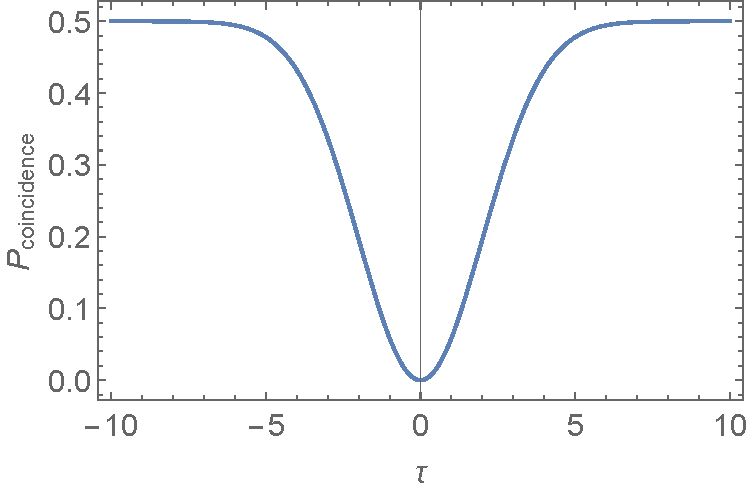
\includegraphics[width=0.47\textwidth]{HOM_dip}
\caption{Hong-Ou-Mandel dip for two photons with normal Gaussian temporal distribution functions, and temporal offset $\tau$ between them. $\tau$ effectively characterises the degree of photon distinguishability, where \mbox{$\tau=0$} represents complete indistinguishability (quantum statistics), and \mbox{$\tau\to\pm\infty$} represents complete distinguishability (classical statistics). Thus, performing this experiment and measuring $P_\text{coincidence}$ can be used to characterise the degree of photon distinguishability.} \label{fig:HOM_dip}\index{Hong-Ou-Mandel dip}
\end{figure}

In the above representation of mode-mismatch as a temporal or spatial translation, the process is entirely coherent, and could in principle be reversed if the translation were known (which might easily be established using tomographic characterisation techniques). Of course, such translations could occur incoherently also. In particular, `time-jitter' is where this process occurs incoherently, and the photons are subject to probabilistic temporal displacements. In this instance, a pure single-photon state would evolve into a mixture of states subject to different displacements. Since the mode-mismatch is now probabilisitic, it is not reversible. The state of a single photon subject to time-jitter would be of the form,
\begin{align}\index{Time-jitter}
\hat\rho_\text{jitter} = \int_{-\infty}^\infty p_\text{jitter}(\Delta_t) \ket{\psi-\Delta_t}\bra{\psi-\Delta_t}d\Delta_t,
\end{align}
where $p_\text{jitter}(\Delta_t)$ characterises the classical probability distribution of the temporal displacement. Time-jitter is particularly natural in heralded spontaneous parametric down-conversion (SPDC) sources (Sec.~\ref{sec:single_phot_src}), where imprecision in the measurement time of the heralding mode projects that temporal uncertainty onto the heralded state. For this reason, much time is being invested into engineering SPDC sources with separable output photons, such that pathological behaviour of the detection of the heralding photon does not project the heralded photon onto a mixed state. Time-jitter is a major consideration in all present-day single-photon source technologies.

When considering mode-mismatch, there are two general regimes for how it manifests itself in an optical system. The first is when the interference taking place is between distinct, independent photons, i.e HOM interference (or its equivalent generalisations to higher-photon-number systems). The second is when multiple paths followed by a given photon interfere it with itself, i.e Mach-Zehnder (MZ)\index{Mach-Zehnder (MZ) interference} interference. The former only requires mode-matching on the scale of the photons' wave-packets, whereas the latter requires interferometric stability on the order of the photons' wavelength, a far more demanding requirement. This is discussed in greater detail in Sec.~\ref{sec:opt_stab}.

Mode-mismatch has been studied extensively in the context of linear optics quantum computing (LOQC), introduced in Sec.~\ref{sec:KLM_univ}. In particular, it was shown that in the cluster state formalism (Sec.~\ref{sec:CSQC}), mode-mismatch in a fusion gate is equivalent to a dephasing error model, where the dephasing rate is related to the degree of photon distinguishability (i.e visibility) \cite{bib:RohdeRalph06}. More generally, the operation of entangling gates \cite{bib:RohdeFreqTemp05, bib:RohdeGateChar05, bib:RohdeOptPhot05, bib:RohdeTimeRes11} and \textsc{BosonSampling} \cite{bib:RohdeArbSpec15, bib:RohdeArbLow12} have been considered, and explicit error models derived.

%
% Dispersion
%

\subsection{Dispersion} \label{sec:dispersion}\index{Dispersion}

Dispersion is the phenomenon of frequency-dependent velocity of light in a given medium. These effects can be very diverse, but can always be expressed in the mode-operator representation using an appropriate transformation in the temporal or spectral wavefunction,
\begin{align}
f_\text{disp}: \,\tilde\psi(\omega)\to\tilde\psi(\omega)'.
\end{align}

%
% Spectral Filtering
%

\subsection{Spectral filtering} \label{sec:spectral_filt} \index{Spectral filtering}

In Sec.~\ref{sec:eff_err} we discussed the loss channel, whereby with some fixed probability photons are lost to the environment. In reality, this process is often not uniform, but frequency-dependent, resulting in spectral filtering effects. For example, optical fibres are typically designed to operate with a particular optical frequency in mind, and will attenuate frequencies outside a given range, implementing, for example, low-pass, high-pass or band-pass spectral filtering.

Because spectral filtering can be regarded as frequency-dependent loss, it can be modelled in the same way as per the loss channel, but using a frequency-dependent beamsplitter with transmissivity $\eta_f(\omega)$, which models the frequency response of the channel. The model is shown in Fig.~\ref{fig:spectral_filter_model}.

\begin{figure}[!htb]
	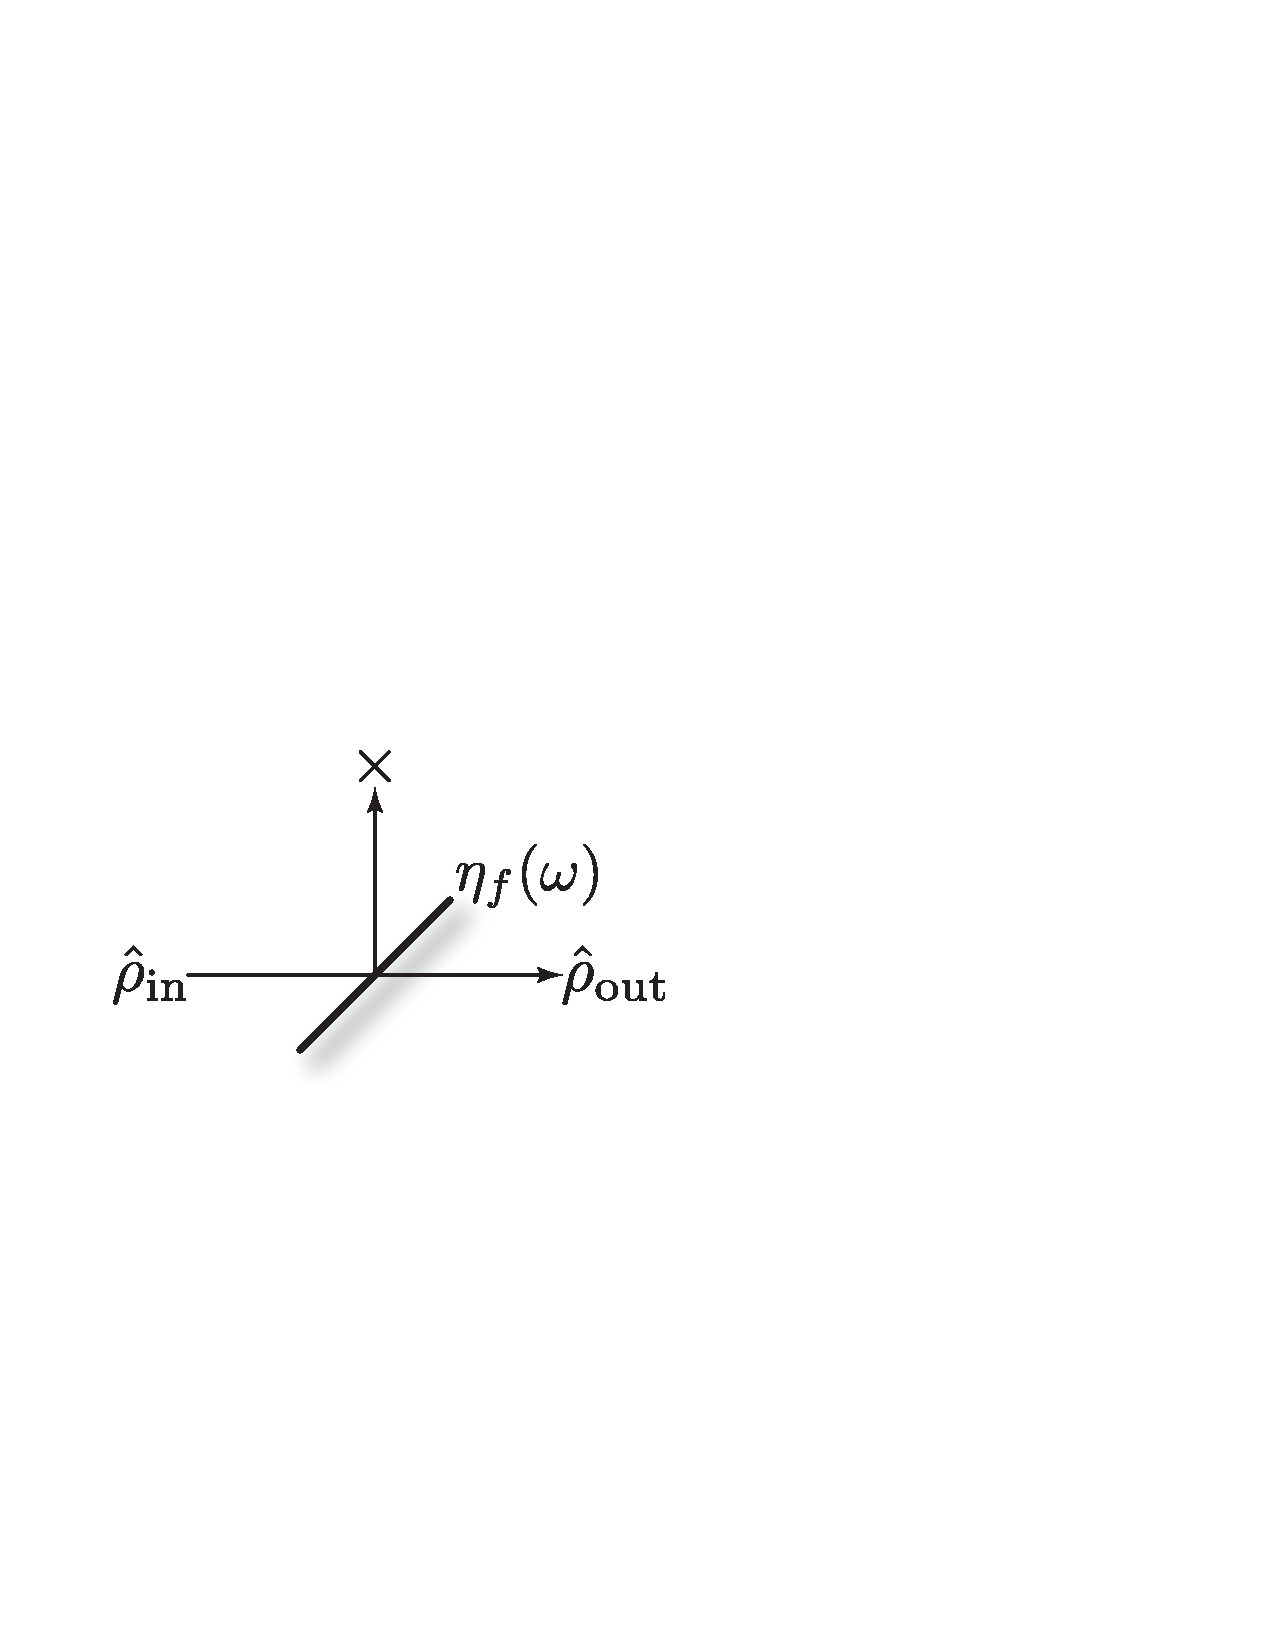
\includegraphics[width=0.25\textwidth]{spectral_filter_model}
	\caption{Model for the spectral filtering channel. The input state, $\hat\rho_\text{in}$, passes through a beamsplitter of frequency-dependent transmissivity $\eta_f(\omega)$, and the reflected mode discarded, yielding the lossy output state \mbox{$\hat\rho_\text{out} = \mathcal{E}^\text{filter}_{\eta_f}(\hat\rho_\text{in})$}.} \label{fig:spectral_filter_model} \index{Spectral filtering}
\end{figure}

This channel has the effect of modulating the spectral distribution function of a photonic mode operator $\hat{A}_\psi^\dag$ to $\hat{A}_{\psi'}^\dag$, where,
\begin{align}
\psi'(\omega) = \sqrt{\eta_f(\omega)}\psi(\omega).	
\end{align}
Note that unless \mbox{$\eta_f(\omega)=1\,\forall\,\,\psi(\omega)\neq 0$}, the new distribution function $\psi'(\omega)$ will not be normalised, where the normalisation reflects the loss probability,
\begin{align}
p_\text{loss} = 1 - \int_{-\infty}^\infty \eta_f(\omega)|\psi(\omega)|^2\,d\omega.
\end{align}

%
% Phase-Space
%

\subsection{Phase-space} \index{Phase-space errors}

In Sec.~\ref{sec:non_lin_opt} we introduce the displacement and squeezing operations, two non-linear operations which are important ingredients in CV quantum information processing schemes. Of course, such processes are subject to errors.

In the case of the displacement operation, which is implemented by mixing a state with a coherent state on a beamsplitter, errors in the amplitude of the coherent state or in the beamsplitter reflectivity will introduce an offset in the displacement amplitude. Thus, instead of implementing $\hat{D}(\alpha)$, we might over- or under-displace the state, implementing \mbox{$\hat{D}(\Delta)\hat{D}(\alpha)\propto \hat{D}(\alpha+\Delta)$}, for some error $\Delta$.

In the case of the squeezing operation, we might similarly have uncertainty in the squeezing parameter, thus implementing $\hat{S}(\xi+\Delta)$ instead of $\hat{S}(\xi)$.
\sketch{sketch_12}

\latinquote{Igne natura renovatur integra.}

%
% Cost Vector Analysis
%

\section{Quantum cost vector analysis} \label{sec:quantum_meas_cost}
\index{Costs}\index{Attributes}\index{Cost vector analysis}

\dropcap{A}{s} with the classical case in Sec.~\ref{sec:costs}, there will be costs associated with the links and nodes in a network -- nothing is free! In the quantum case, all the usual classical costs are valid, but there are some very important additions of far greater relevance to most quantum applications. Classical digital data is discretised, resulting in data transmission highly robust against noise. In a quantum setting this is necessarily not the case, as the coefficients in quantum superpositions are continuous, meaning that errors accumulate during transmission and states will inevitably deteriorate, unlike digital states. This requires a rethinking of appropriate cost metrics.

%
% Costs
%

\subsection{Costs}

We now briefly introduce some of the key measures for quantifying the quality of quantum communications links, and how they may be expressed as metrics with meaningful operational interpretations. Many of the measures typically employed for characterising quantum systems are not true metrics (i.e costs), but in many cases can be converted to metrics, or used meaningfully as attributes instead.

%
% Efficiency
%

\subsubsection{Efficiency} \index{Loss channel}

The efficiency measure introduced previously is multiplicative, so for consecutive lossy channels the net efficiency is,
\begin{align}
\eta_\mathrm{net}=\prod_i \eta_i,
\end{align}
where $\eta_i$ is the efficiency of the $i$th channel. Intuitively, this is simply telling us that if a photon passes through a channel with success probability $\eta_1$, followed by another with $\eta_2$, the total success probability is \mbox{$\eta_1\eta_2$}.

When employing single-photon encoding of qubits (e.g using the polarisation degree of freedom), there are three basis states of interest: a single photon horizontally polarised ($\ket{H}$); a single photon vertically polarised ($\ket{V}$); and, the vacuum state ($\ket{0}$). The effect of the loss channel on this type of state is to map $\ket{H}$ and $\ket{V}$ to $\ket{\mathrm{0}}$ with probability \mbox{$1-\eta$}, while doing nothing to $\ket{\mathrm{0}}$. Note that because the loss process affects both logical basis states ($\ket{H}$ and $\ket{V}$) identically, its action is invariant under unitary operations in the logical (i.e polarisation) basis space.

%
% Spectral filtering
%

\subsubsection{Spectral filtering} \index{Loss channel}\index{Spectral filtering}

Because spectral filtering can be regarded as a frequency-dependent loss channel, its associated cost can be treated in the same manner, except that rather than keeping track of a single efficiency $\eta$, we track a frequency response function $\eta_f(\omega)$, with the same multiplicative property,
\begin{align}
	\eta_f^\mathrm{(net)}(\omega)=\prod_i \eta_f^{(i)}(\omega).
\end{align}

If we are keeping track of the frequency response, the usual efficiency metric can be made redundant and absorbed into the frequency response function as a uniform response,
\begin{align}
	\eta_f(\omega)=\eta\,\,\forall\,\omega.
\end{align}

%
% Decoherence
%

\subsubsection{Decoherence} \index{Dephasing channel} \index{Depolarising channel} \index{Decoherence}

The dephasing and depolarising channels, given by Eqs.~(\ref{eq:dephasing_channel},\ref{eq:depolarizing_channel}), also behave multiplicatively. If $p_i$ is the probability that the state passing through the $i$th channel in series does not undergo the error process, then the probability of the state passing though the entire series without error is simply,
\begin{align}
p_\mathrm{net}=\prod_i p_i,
\end{align}
exhibiting the same multiplicative behaviour as the loss channel. The same observation applies to any of the other Pauli error channels.

%
% Mode-Mismatch
%

\subsubsection{Mode-mismatch} \index{Mode-mismatch}

In Sec.~\ref{sec:MM_error} we introduced a simple model for temporal mode-mismatch as a displacement in the temporal wave-function of photons propagating through a channel. Clearly, such a process is cumulative -- a temporal displacement of $\Delta_1$ followed by another of $\Delta_2$ yields a net displacement of \mbox{$\Delta_1+\Delta_2$}. Thus, for a chain of such channels we simply accumulate a net temporal displacement of,
\begin{align}
\Delta_\mathrm{net} = \sum_i \Delta_i.
\end{align}

For an incoherent mode-mismatching process, such as time-jitter, an upper bound on the accumulated mismatch may be obtained by summing the maximum temporal displacements at each step.

%
% Distance Measures
%

\subsubsection{Distance measures} \label{sec:fid_metric} \index{Distance measures}

The fidelity of two states directly quantifies how close they are to one another in a geometric sense, i.e on the Bloch sphere \cite{???}, or, in the context of a state passing through a quantum channel, a measure of how well the state is preserved.

The fidelity\index{Fidelity} between two states is defined as,
\begin{align}
\mathcal{F}(\hat\rho_1,\hat\rho_2) = \mathrm{tr}\left(\sqrt{\hat\rho_1^{1/2}\cdot\hat\rho_2\cdot\hat\rho_1^{1/2}}\right),
\end{align}
where,
\begin{align}
& \mathcal{F}(\hat\rho_1,\hat\rho_2) = \mathcal{F}(\hat\rho_2,\hat\rho_1), \nonumber \\
& 0\leq \mathcal{F}(\hat\rho_1,\hat\rho_2) \leq 1.
\end{align}
\mbox{$\mathcal{F}(\hat\rho_1,\hat\rho_2)=1$} iff the states are equal, and \mbox{$\mathcal{F}(\hat\rho_1,\hat\rho_2)=0$} iff they are orthogonal.
In the case where one of the states is a pure state, this simplifies to,
\begin{align}
\mathcal{F}(\hat\rho_1,\ket{\psi_2}) = \bra{\psi_2}\hat\rho_1\ket{\psi_2},
\end{align}
and when both states are pure to simply,
\begin{align}
\mathcal{F}(\ket{\psi_1},\ket{\psi_2}) = |\langle\psi_1 | \psi_2\rangle|^2.
\end{align}

The fidelity is invariant under a common unitary applied to both states,
\begin{align}
\mathcal{F}(\hat\rho_1,\hat\rho_2) = \mathcal{F}(\hat{U}\hat\rho_1 \hat{U}^\dag,\hat{U} \hat\rho_2\,\hat{U}^\dag).
\end{align}

We define the fidelity of two processes, the process fidelity \index{Fidelity} \cite{bib:Gilchrist05}, to be the fidelity between two identical copies of a state that have been evolved under each of those processes, minimised over all possible states. That is, it provides a lower bound on the fidelity between identical states evolved under the two processes. In the context of networking, where quality must be guaranteed, this definition is more appropriate than, say, the average case fidelity. Specifically,
\begin{align}
\mathcal{F}(\mathcal{E}_1,\mathcal{E}_2) = \mathrm{tr}\left( \sqrt{\chi_1^{1/2}\cdot\chi_2\cdot\chi_1^{1/2}}\right),
\end{align}
where $\chi_1$ and $\chi_2$ are the process matrices\index{Process matrices} for $\mathcal{E}_1$ and $\mathcal{E}_2$.

The fidelity of two processes is invariant under a common unitary applied to both channels before or after the process. Specifically,
\begin{align}
\mathcal{F}(\mathcal{E}_1,\mathcal{E}_2) &= \mathcal{F}(\mathcal{E}_U\circ\mathcal{E}_1,\mathcal{E}_U\circ\mathcal{E}_2) \nonumber \\
&= \mathcal{F}(\mathcal{E}_1\circ \mathcal{E}_U,\mathcal{E}_2\circ \mathcal{E}_U),
\end{align}
where $\mathcal{E}_U$ is an arbitrary unitary process.

In the special case of an identity channel, $\hat{\mathbb{I}}$, which is of special interest in many communications scenarios, we employ the shorthand,
\begin{align}
\mathcal{F}(\mathcal{E}) = \mathcal{F}(\mathcal{E},\hat{\mathbb{I}}) = \min_{\hat\rho} \left[\mathcal{F}(\hat\rho,\mathcal{E}(\hat\rho))\right].
\end{align}
By definition \mbox{$\mathcal{F}(\mathcal{E})=1$} iff \mbox{$\mathcal{E}=\hat{\mathbb{I}}$}.

A lower bound on the process fidelity of multiple processes in series is multiplicative,
\begin{align}
\mathcal{F}(\mathcal{E}_2\circ\mathcal{E}_1,\mathcal{E}_3) &\geq \mathcal{F}(\mathcal{E}_2,\mathcal{E}_3)\cdot\mathcal{F}(\mathcal{E}_1,\mathcal{E}_3), \nonumber \\
\mathcal{F}(\mathcal{E}_2\circ\mathcal{E}_1) &\geq \mathcal{F}(\mathcal{E}_2)\cdot\mathcal{F}(\mathcal{E}_1).
\end{align}

Generalising to a sequence of $n$ processes in series yields,
\begin{align}
\mathcal{F}(\mathcal{E}_n\circ\dots\circ\mathcal{E}_1) \geq \prod_{i=1}^n \mathcal{F}(\mathcal{E}_i).
\end{align}

An alternate measure for the distance between two quantum states is the trace-norm distance\index{Trace-norm distance}, defined as,
\begin{align}
D(\hat\rho_1,\hat\rho_2) &= \frac{1}{2}\|\hat\rho_1 - \hat\rho_2\|_1 \nonumber\\
&= \frac{1}{2}\sum_i |\lambda_i|,
\end{align}
where $\lambda_i$ are the eigenvalues of \mbox{$\hat\rho_1-\hat\rho_2$}. Like the fidelity, the trace-norm distance is invariant under unitary transformation. Furthermore, it is contractive under the action of quantum processes,
\begin{align}
D(\mathcal{E}(\hat\rho_1),\mathcal{E}(\hat\rho_2)) \leq D(\hat\rho_1,\hat\rho_2).
\end{align}
The trace-norm distance relates to the fidelity according to the following bounds,
\begin{align}
1-F(\hat\rho_1,\hat\rho_2) \leq D(\hat\rho_1,\hat\rho_2) \leq \sqrt{1-F(\hat\rho_1,\hat\rho_2)^2}.
\end{align}

%
% Purity
%

\subsubsection{Purity} \index{Purity}

The purity of a state that was initially pure quantifies how well quantum coherence was maintained during evolution, equivalently how well superpositions are maintained. The purity is defined as,
\begin{align}
\mathcal{P}(\hat\rho) = \mathrm{tr}(\hat\rho^2),
\end{align}
where,
\begin{align}
\frac{1}{\mathrm{dim}(\hat\rho)} \leq \mathcal{P}(\hat\rho) \leq 1.
\end{align}
We have \mbox{$\mathcal{P}(\hat\rho) = 1$} iff \mbox{$\hat\rho=\ket{\psi}\bra{\psi}$} is a pure state, and \mbox{$\mathcal{P}(\hat\rho)=1/\mathrm{dim}(\hat\rho)$} iff \mbox{$\hat\rho=\mathbb{\hat{I}}/\mathrm{dim}(\hat\rho)$} is the maximally mixed state.

The purity is invariant under unitary operations,
\begin{align}
\mathcal{P}(\hat\rho) = \mathcal{P}(\hat{U}\hat\rho\,\hat{U}^\dag).
\end{align}

The purity of a process is defined analogously to the fidelity of a process,
\begin{align}
\mathcal{P}(\mathcal{E}) = \mathrm{tr}(\chi^2),
\end{align}
and as with the fidelity, a lower bound on the purity of multiple processes in series is multiplicative,
\begin{align}
\mathcal{P}(\mathcal{E}_2\circ\mathcal{E}_1)
\geq \mathcal{P}(\mathcal{E}_2)\cdot\mathcal{P}(\mathcal{E}_1).
\end{align}
\comment{CHECK THIS!}. If the channel implements a unitary operation then necessarily \mbox{$\mathcal{P}(\mathcal{E})=1$}.

Like the process fidelity, the purity of a quantum process is invariant under unitary operations,
\begin{align}
\mathcal{P}(\mathcal{E}) &= \mathcal{P}(\mathcal{E}_U\circ\mathcal{E}) \nonumber \\
&= \mathcal{P}(\mathcal{E}\circ\mathcal{E}_U).
\end{align}

Generalising to a sequence of $n$ processes in series yields,
\begin{align}
\mathcal{P}(\mathcal{E}_n\circ\dots\circ\mathcal{E}_1) \geq \prod_{i=1}^n \mathcal{P}(\mathcal{E}_i).
\end{align}

%
% Entanglement
%

\subsubsection{Entanglement} \label{sec:ent_meas} \index{Entanglement measures}

When distributing entanglement between separate nodes, metrics quantifying bipartite entanglement are relevant. For pure bipartite states $\ket{\psi}_{A,B}$, the purity of one of the reduced subsystems directly quantifies the degree of entanglement between them,
\begin{align}
\mathcal{M}(\ket{\psi}_{A,B})) &= \mathcal{P}(\mathrm{tr}_A(\ket{\psi}_{A,B})) \nonumber \\
&= \mathcal{P}(\mathrm{tr}_B(\ket{\psi}_{A,B})),
\end{align}
The entanglement between two systems in invariant under local unitaries,
\begin{align}
\mathcal{M}(\ket{\psi}_{A,B}) = \mathcal{M}([\hat{U}_A\otimes \hat{U}_B]\ket{\psi}_{A,B}).
\end{align}

%
% Phase-Space
%

\subsubsection{Phase-space} \index{Phase-space errors}

Displacements in phase-space accumulate additively, up to a phase-factor. Specifically, the composition of two displacements is given by,
\begin{align}
\hat{D}(\alpha)\hat{D}(\beta) = e^{\frac{1}{2}(\alpha\beta^*-\alpha^*\beta)}\hat{D}(\alpha+\beta).
\end{align}
Thus, the composition of a chain of unwanted or uncertain displacements yields, up to phase, a displacement with amplitude given by the sum of the individual displacement amplitudes.

Similarly, from the definition of the squeezing operator,
\begin{align}\label{eq:sq_op}
\hat{S}(\xi) = \exp\left[ \frac{1}{2}(\xi^*\hat{a}^2 - \xi{\hat{a}^{\dag 2}})\right],
\end{align}
it is evident that squeezing accumulates additively as well,
\begin{align}
\hat{S}(\xi_1)\hat{S}(\xi_2) = \hat{S}(
\xi_1+\xi_2).	
\end{align}

%
% Channel Capacity
%

\subsubsection{Channel capacity} \label{sec:channel_cap} \index{Channel capacity}

The measures considered until now have quantified the preservation of quantum states. Alternately, one might consider information theoretic measures, which quantify the number of bits/qubits transmitted by a link, i.e the number of bits/qubits in common before and after the channel. This is an extremely powerful tool as it upper bounds the amount of information the receiver can extract from the transmitter under \textit{any} measurement scheme, very useful in a cryptographic context, where we want security to be attack-independent\index{Information-theoretic security} (Sec.~\ref{sec:comp_vs_inf_th_sec}).

The Shannon entropy \cite{???} of a classical probability distribution $X$ is given by,
\begin{align}\index{Shannon entropy}
H(X) = -\sum_x p_x\log_2(p_x),
\end{align}
where $p_x$ are the probabilities in the distribution. For a joint distribution over $X$ and $Y$ this simply generalises to,
\begin{align}\index{Joint Shannon entropy}
H(X,Y) =  -\sum_{x,y} p_{x,y}\log_2(p_{x,y})
\end{align}

The von Neuman entropy \cite{???} for quantum density operators, $S(\hat\rho)$, is defined analogously, replacing probabilities with density operator eigenvalues,
\begin{align}\index{von Neuman entropy}
S(\hat\rho) &= - \sum_x \lambda_x \log_2 (\lambda_x) \nonumber \\
&= -\mathrm{tr}(\hat\rho\,\log \,\hat\rho),
\end{align}
where $\{\lambda\}$ is the eigenvalue spectrum of $\hat\rho$. This modification is logically justified, as the eigenvalues can be interpreted directly as a purely classical probability distribution of orthogonal states when the density operator is transformed into a basis with no coherences between basis states (i.e a diagonal basis or spectral decomposition). In that case the Shannon and von Neuman entropies essentially have identical physical interpretations.

The \textit{mutual information} specifies the number of bits in common between two distributions. Equivalently, it is the maximum number of bits that one party can learn about the other. For two classical distributions, $A$ and $B$, this is given by,
\begin{align}\index{Mutual information}
I(A;B) = H(A) + H(B) - H(A,B).
\end{align}
Equivalently, for density operators,
\begin{align}
I(\hat\rho_A;\hat\rho_B) = S(\hat\rho_A) + S(\hat\rho_B) - S(\hat\rho_A,\hat\rho_B),
\end{align}
using the von Neuman entropy. The mutual information between two quantum states is invariant under local unitary transformations,
\begin{align}
I(\hat\rho_A;\hat\rho_B) = I(\hat{U}_A\hat\rho_A \hat{U}_A^\dag; \hat{U}_B\hat\rho_B \hat{U}_B^\dag),
\end{align}
since the eigenvalue spectrum of a density operator is invariant under unitary transformations. Therefore, the mutual information represents the maximum amount of information Bob can learn about Alice's state under \textit{any} local operations.

A quantum process cannot increase the mutual information between two parties. This yields the \textit{data processing inequality}\index{Data processing inequality} that, for a sequence of channels \mbox{$X\to Y\to Z$},
\begin{align}\index{Data processing inequality}\label{eq:data_proc_ineq}
I(X:Z)&\leq I(X:Y), \nonumber \\
I(X:Z)&\leq I(Y:Z),
\end{align}
with equality if and only if the channel not specified in the identity on the right hand side (\mbox{$Y\to Z$} or \mbox{$X\to Y$} respectively) is unitary, i.e one of the links in the chain perfectly preserves information content. The progression is shown in Fig.~\ref{fig:data_proc_ineq}.

\begin{figure}[!htbp]
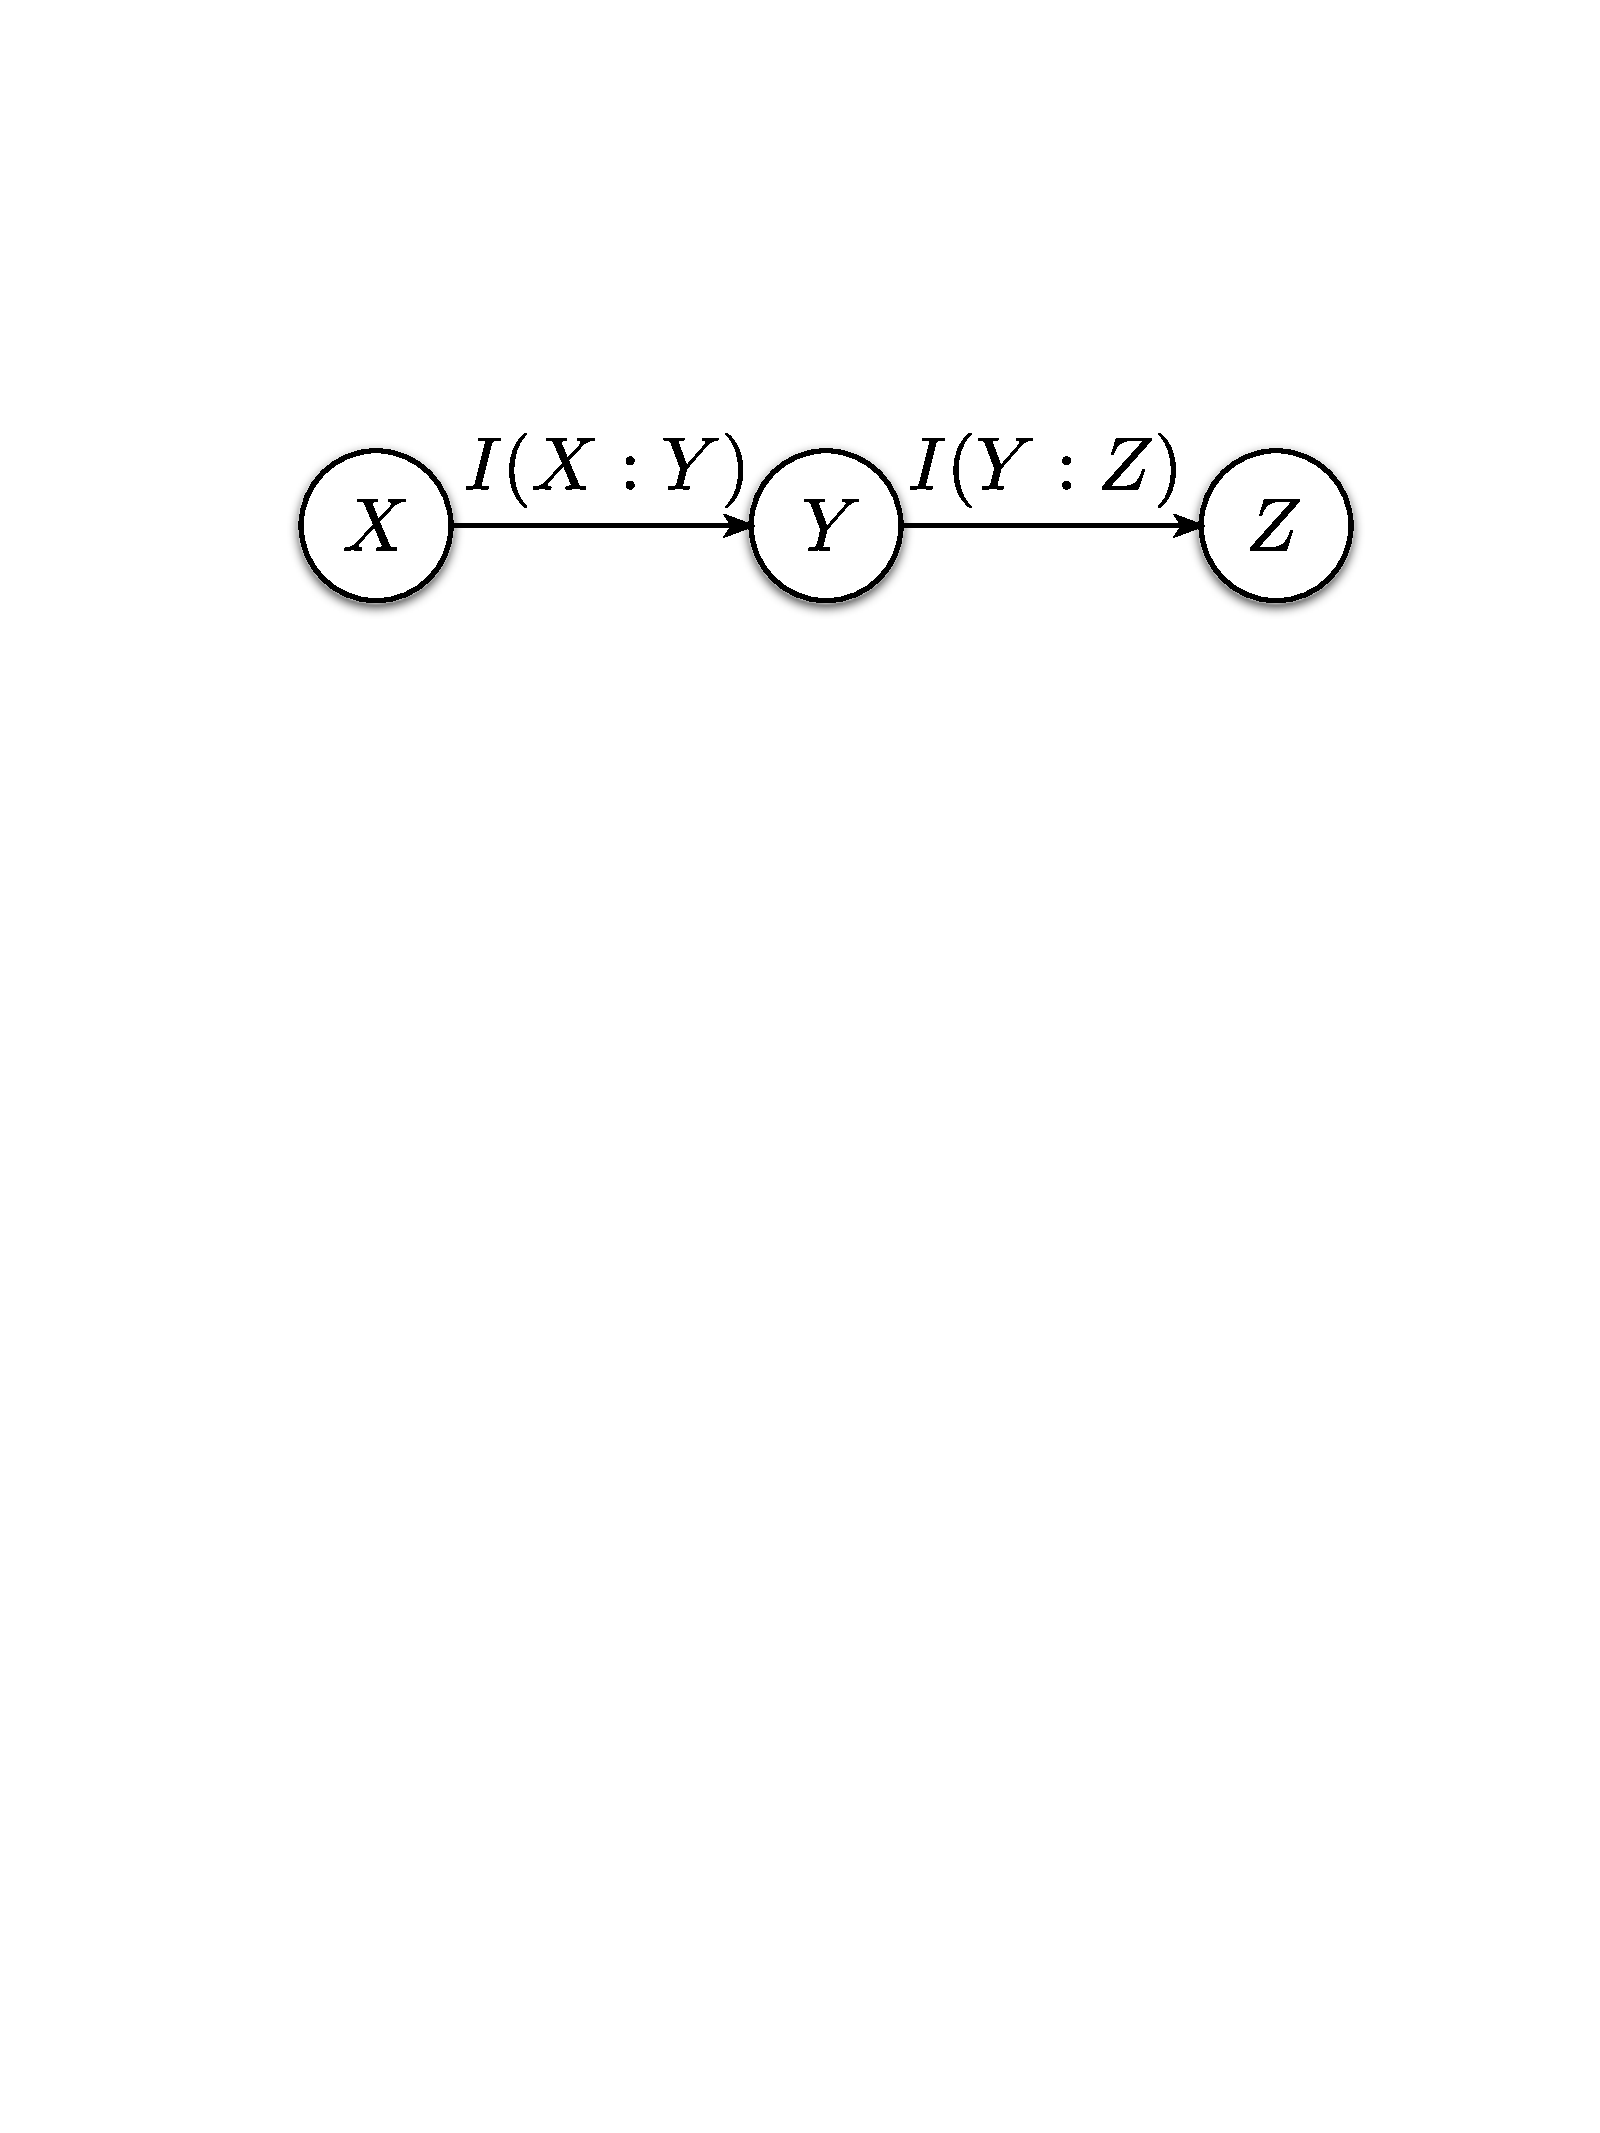
\includegraphics[width=0.3\textwidth]{data_proc_ineq}
\caption{A sequence of events \mbox{$X\to Y\to Z$}. The data processing inequality states that the mutual information from beginning to end is upper-bounded by the mutual information between neighbouring stages, as per Eq.~(\ref{eq:data_proc_ineq}).}\label{fig:data_proc_ineq}	
\end{figure}

The mutual information is defined as being between a particular known pair of states. Of course, in a quantum network we will seldom know what the states being communicated are and will therefore be unable to directly calculate the mutual information. To address this, the \textit{classical channel capacity}\index{Classical channel capacity} of a channel is defined as,
\begin{align}\index{Channel capacity}
\mathcal{C}(\mathcal{E}) = \max_{\hat\rho} [I(\hat\rho,\mathcal{E}(\hat\rho))],
\end{align}
with the intuitive interpretation as the maximum mutual information between input and output states that can be achieved for the channel. (Note: this definition of `capacity' is not to be confused with that which we later refer to in flow networks).

Analogous to the mutual information for classical systems is the \textit{coherent information} for quantum systems \cite{bib:PhysRevA.54.2629}, defined as,
\begin{align}\index{Coherent information}
I(\hat\rho,\mathcal{E}) = S(\mathcal{E}(\hat\rho)) - S_e(\hat\rho,\mathcal{E}).
\end{align}
Here $S_e$ is the \textit{exchange entropy}, a measure of how much information is exchanged between the state $\hat\rho$ and the environment under the action of the process. Specifically, it is given by the entropy of the environment subsystem in Eq.~(\ref{eq:proc_environment}), after application of the channel. This yields the intuitive interpretation that the coherent information is the information contained in the evolved state, discounted by the amount lost to the environment.

The quantum coherent information exhibits much of the same mathematical structure as the classical mutual information. And analogously, we can define the \textit{quantum channel capacity} as,
\begin{align}\index{Quantum channel capacity}
\mathcal{Q}(\mathcal{E}) = \max_{\hat\rho} I(\hat\rho,\mathcal{E}).
\end{align}

Analytic solutions to $\mathcal{C}(\mathcal{E})$ and $\mathcal{Q}(\mathcal{E})$ are not known even for simple Pauli error channels such as dephasing and depolarisation. However, once net dephasing or depolarisation rates have been calculated across a route, the channel capacities can easily be solved numerically, which is sufficient for the numerical algorithms we will rely upon, where a number representing \textit{cost}, rather than an analytic solution, is all we need.

\comment{Add stuff on channel capacities of different channels, like Pauli error channels etc.}

%
% Latency
%

\subsubsection{Latency} \label{sec:latency_metric} \index{Latency}

Aside from the actual information content of a transmitted quantum state, the latency associated with its transmission is a key consideration in many time-critical applications.

By defining the latency of a link/node as the time between receipt of a quantum state and its retransmission, the total latency of a route is simply the sum of all the individual node and link latencies across the route,
\begin{align}
\mathcal{L}(R) = \sum_{i\in R} \mathcal{L}_i,
\end{align}
where $\mathcal{L}_i$ is the latency associated with the $i$th link in route $R$.

%
% Dollars
%

\subsubsection{Dollars} \label{sec:dollars} \index{Dollar cost}

Not to be overlooked is the actual dollar cost of communicating information. It is unlikely that Alice and Bob outright own the entire infrastructure of particular routes. Rather, different links and nodes are likely to be owned by different operators (particularly in ad hoc networks), who are most likely going to charge users for bandwidth in their network (quantum networks won't be cheap). Clearly dollar costs are additive over the links and nodes within routes,
\begin{align}
\mathcal{C}(R) = \sum_{i\in R} \mathcal{C}_i,
\end{align}
where $\mathcal{C}_i$ is the dollar cost of utilising the $i$th link in route $R$.

%
% Costs as Distance Metrics
%

\subsection{Costs as distance metrics} \label{sec:cost_as_dist} \index{Cost distance metrics}

Def.~\ref{def:metric} defines the properties of a cost metric in the classical context. We now wish to consider this in the quantum context.

If we consider a lossy photonic channel for example, efficiencies ($\eta$) are multiplicative -- for a route \mbox{$v_1\to v_2\to v_3$}, the net efficiency is given by the product of the individual efficiencies, \begin{align}
\eta_{v_1\to v_2 \to v_3} = \eta_{v_1\to v_2} \eta_{v_2\to v_3}.
\end{align}
This is multiplicative rather than additive, clearly not satisfying our definition for a cost metric. However, multiplicative metrics\index{Multiplicative metrics} such as this can easily be made additive\index{Additive metrics} by shifting to a logarithmic scale, since
\begin{align}\index{Logarithmic scale}
\log(\eta_{v_1\to v_2\to v_3}) = \log(\eta_{v_1\to v_2}) + \log(\eta_{v_2\to v_3}),
\end{align}
which now has a legitimate interpretation as a distance. The same applies to, for example, frequency response functions, which are equivalent to frequency-dependent loss.

In general, for a series of links \mbox{$v_1\to v_2 \to \dots \to v_n$} characterised by multiplicative measure $m$, the equivalent cost metric is,
\begin{align} \label{eq:dist_log}\index{Logarithmic distance}
c_{v_1\to v_2 \to \dots \to v_n} = -\sum_{i=1}^{n-1} \log (m_{v_i\to v_{i+1}}).
\end{align}
We have assumed that \mbox{$0\leq m \leq 1$}, where \mbox{$m=0$} represents complete failure, and \mbox{$m=1$} represents ideal operation.

With these properties, the costs in our graph have an elegant interpretation. In the case of perfect operation, \mbox{$m=1$}, the cost is \mbox{$c=0$}, creating an ideal direct link between neighbouring nodes at no cost. On the other hand for complete failure, \mbox{$m=0$}, the cost metric is \mbox{$c=\infty$}, effectively removing the link from the network and prohibiting pathfinding algorithms from following that route altogether.

Such a logarithmic scale is particularly convenient when a cost metric over links accumulates on a per physical distance basis, in which case the cost metric is simply the physical length of the link multiplied by the metric per unit distance. For example, if a fibre channel implements loss at 3dB/km, the loss over 10km is 10$\times$3dB.

Note that lower bounds on fidelity, purity, efficiency and dephasing are all multiplicative on a scale of 0 to 1, and thus their logarithms may be regarded as cost metrics. Spatio-temporal mode-mismatch, latency, dollar cost and displacements are clearly automatically metrics as they are additive.

A dephasing channel can be easily converted to a distance metric as follows. First we reparameterise the dephasing channel into,
\begin{align}
\mathcal{E}(\hat\rho) &= p\hat\rho + (1-p)\hat{Z}\hat\rho\hat{Z}\nonumber\\
&= (2p-1)\hat\rho + (1-p)(\hat{Z}\hat\rho\hat{Z} + \hat\rho).	
\end{align}
Now \mbox{$2p-1$} is the probability that the state is not dephased and \mbox{$1-p$} is the probability that the state is replaced with the completely dephased state. Therefore the probability of multiple applications of the channel not dephasing the state scales multiplicitavely as,
\begin{align}
p_\mathrm{no\, error} = \prod_{i}(2p_i-1),
\end{align}
which is additive in a logarithmic scale as before,
\begin{align}
\log(p_\mathrm{no\, error}) = \sum_i \log(2p_i-1),
\end{align}
which acts as a distance metric. This approach can similarly be applied to other Pauli channels.


In the case of mutual information and channel capacity, it makes most sense to consider the number of bits that are lost by a channel, rather than the number communicated, since then we have a measure with quasi-metric properties. Specifically, let the number of bits lost by a channel be the difference between the number of bits in the input state and the channel capacity,
\begin{align}
B_\mathrm{lost}(\mathcal{E},\hat\rho) = S(\hat\rho) - \mathcal{C}(\mathcal{E}).
\end{align}
Then there are two cases to consider -- upper and lower bounds on accumulated lost bits.

The best-case scenario is that subsequent channels lose the same bits, giving us a lower bound on the number of lost bits as the maximum number of bits lost by the constituent channels,
\begin{align}
B_\mathrm{lower}(\mathcal{E}_2\circ\mathcal{E}_1,\hat\rho) = \mathrm{max}[B_\mathrm{lost}(\mathcal{E}_1,\hat\rho), B_\mathrm{lost}(\mathcal{E}_2,\hat\rho)].
\end{align}
Alternately, each subsequent channel could lose a different set of bits, in which case the number of lost bits accumulates additively,
\begin{align}
B_\mathrm{upper}(\mathcal{E}_2\circ\mathcal{E}_1,\hat\rho) = B_\mathrm{lost}(\mathcal{E}_1,\hat\rho) + B_\mathrm{lost}(\mathcal{E}_2,\hat\rho). 
\end{align}
Then, the number of actual bits lost is bounded from above and below as,
\begin{align}
B_\mathrm{lower} \leq B_\mathrm{lost} \leq B_\mathrm{upper}.	
\end{align}

%In the case of mutual information, which is not a metric, one can use it to define the \textit{variation of information} metric,
%\begin{align}\index{Variation of information}
%d_\mathrm{VI}(X,Y) &= H(X,Y) - I(X;Y), \nonumber \\
%d_\mathrm{VI}(\hat\rho_A,\hat\rho_B) &= S(\hat\rho_A,\hat\rho_B) - I(\hat\rho_A;\hat\rho_B),
%\end{align}
%or for a channel,
%\begin{align}
%d_\mathrm{VI}(\hat\rho,\mathcal{E}) &= S(\hat\rho,\mathcal{E}(\hat\rho)) - I(\hat\rho;\mathcal{E}(\hat\rho)),
%\end{align}
%which obeys the metric properties.

%
% Non-Trivial Node Operations
%

\subsection{Non-trivial node operations}

Thus far we have considered how to accumulate cost metrics across routes through a network, where each link is subject to some quantum process obeying our notion of a cost metric. But what happens when the links are interspersed with nodes that may be doing more than just simple switching?

A more general scenario to consider is where the nodes are not restricted to routing, but can additionally implement arbitrary unitary operations. This substantially broadens the class of networks under consideration, to encompass nodes capable of doing everything from straightforward routing to entire quantum computations.

All of the examples for cost metrics we introduced in Sec.~\ref{sec:quantum_meas_cost} have the property that they are invariant under unitary operations. Therefore the costs along a route may simply be accumulated as before, summing up the edge weights, without needing any special treatment for node operations, provided they are unitary. For non-unitary node processes, we can merge them into their neighbouring link processes as before (see Fig.~\ref{fig:remove_nodes}).

\subsection{Negative cost vectors}\index{Negative cost vectors}

When we initially introduced cost vector analysis in the classical context (Sec.~\ref{sec:costs}) we insisted that costs be positive by definition. However, in the quantum scenario we will loosen this demand since negative costs arise quite naturally in the context of operations that \textit{improve} quantum data. Specifically this arises naturally when nodes implement operations such as entanglement purification or quantum error correction, to be discussed in detail in Sec.~\ref{sec:QOS_chap}. In that case making what would otherwise be a routing detour can yield net benefit, and so the cost vector analysis must take these negative costs into consideration and give them the favourable treatment they deserve.
\sketch{sketch_13}

\latinquote{Flectere si nequeo superos, acheronta movebo.}

%
% Quantum Transmission Control Protocol (QTCP)
%

\section{Quantum Transmission Control Protocol (QTCP)} \index{Quantum Transmission Control Protocol (QTCP)}\label{sec:QTCP}

\dropcap{I}{n} the classical world, TCP is employed for data transmission and routing. Next we present a simple toy model for a proposed quantum equivalent -- the Quantum Transmission Control Protocol (QTCP). The stack is described in detail in Sec.~\ref{sec:prot_stack}.

We emphasise that this toy model is not intended to be a proposal suited to immediate implementation, solving all the problems of quantum communication in the most effective way. Rather, we simply aim to construct a sketch of the data structures and algorithms that might form a basis for future, more well-considered real-world implementations. Alternately, it is plausible that a QTCP protocol may never reach the light of day at all, instead being made redundant by networks built entirely on entanglement distribution, discussed in detail in Secs.~\ref{sec:rep_net} \& \ref{sec:ent_ultimate}. The answer to this question is difficult to foresee, largely depending on the future requirements of quantum communication protocols.

The goal of QTCP is to abstract away the low-level physical operation of a quantum network to create a virtual interface between Alice and Bob, allowing direct access to data as if it were held locally, in much the same way that high-level services like classical FTP facilitate interaction with remote data as though it were a local asset, blind to the intermediate networking.

The design goals of our elementary toy model are simply to capture the quintessential feature requirements of real-world protocols, and a sketch for their implementation. The designs we present should not be interpreted as a final proposal, but merely as laying a foundation of ideas to build upon.

We consider the scenario where Alice (or a set of Alices) is in possession of some quantum state, which she wishes to communicate to Bob (Bobs), with the aim of optimising some arbitrary cost measure. Bob is no guru and doesn't want to concern himself with how the state was communicated from Alice to himself -- his only concern is that he receives it and that it satisfies quality constraints he and Alice have agreed upon.
 
QTCP is the joint software/hardware stack that facilitates these objectives. QTCP begins by logically separating different levels of network functionality into distinct layers of abstraction. This includes primarily:
\begin{itemize}
	\item Encapsulation of data into packets of quantum information (Secs.~\ref{sec:data_message_layer} \& \ref{sec:packet_layer}).
	\item Cost vector analysis (Sec.~\ref{sec:costs}).
	\item Routing decisions (Secs.~\ref{sec:intro_strat} \& \ref{sec:strategies}).
	\item Reconstruction of communicated quantum states upon receipt (Sec.~\ref{sec:reconstruction_layer}).
	\item Enforcement of quality of service requirements and error correction (Sec.~\ref{sec:reconstruction_layer}).
	\item Providing a high-level virtual interface between end-users, which abstracts away low-level operations (Sec.~\ref{sec:services_apps}).
\end{itemize}

All the while, Alice and Bob, as end-users, ought to be as blind as possible to the lower-level layers, instead only directly interfacing with the highest layer of abstraction, that which provides the virtual interface between end-users.
\sketch{sketch_14}

\latinquote{O derint dum metuant.}

%
% QTCP Protocol Stack
%

\subsection{QTCP protocol stack} \label{sec:prot_stack} \index{QTCP protocol stack}

As with classical networking, our protocols for quantum networks will be separated into distinct layers, each performing a specific set of tasks with different levels of abstraction.

The structure of the protocol stack for QTCP is shown in Fig.~\ref{fig:stack}. In summary, the layers in the protocol stack are, beginning from the lowest level:
\begin{itemize}
\item \textsc{Data (Message)}\index{Data (message) layer}: Raw data (`payload') Alice wishes to transmit to Bob. Comprises both \textsc{Quantum Data}\index{Quantum data layer} and \textsc{Classical Data}\index{Classical data layer}.
\item \textsc{Packet}\index{Packet!Layer}: Decomposition of \textsc{Data} into blocks (\textsc{Packet Data}\index{Packet!Data layer}), and associated classical \textsc{Packet Headers}\index{Packet!Header layer} containing metadata (e.g routing information).
\item \textsc{Strategy}\index{Strategy!Layer}: Construct \textsc{Packet} routing strategies based on a cost optimisation algorithm.
\item \textsc{Transport}\index{Transport layer}: Physical routing of \textsc{Packets} to arrive at their destination, based upon metadata contained in \textsc{Packet Header}. Perform collision detection during transit.
\item \textsc{Reconstruction}\index{Reconstruction layer}: Reconstruct \textsc{Data} from received \textsc{Packets}.
\item \textsc{Quality of Service (QoS)}\index{Quality of service (QoS)!Layer}: Apply QEC and determine whether \textsc{QoS} requirements have been satisfied.
\item \textsc{Services \& Applications}\index{Services \& applications layer}: High-level interface to \textsc{Data} presented to Bob's services and applications. The interface abstracts away lower levels of the protocol stack, presenting Bob with only \textsc{Data} and its associated metadata.
\end{itemize}

\begin{figure}[!htbp]\index{QTCP protocol stack}
\if 2\pubmode
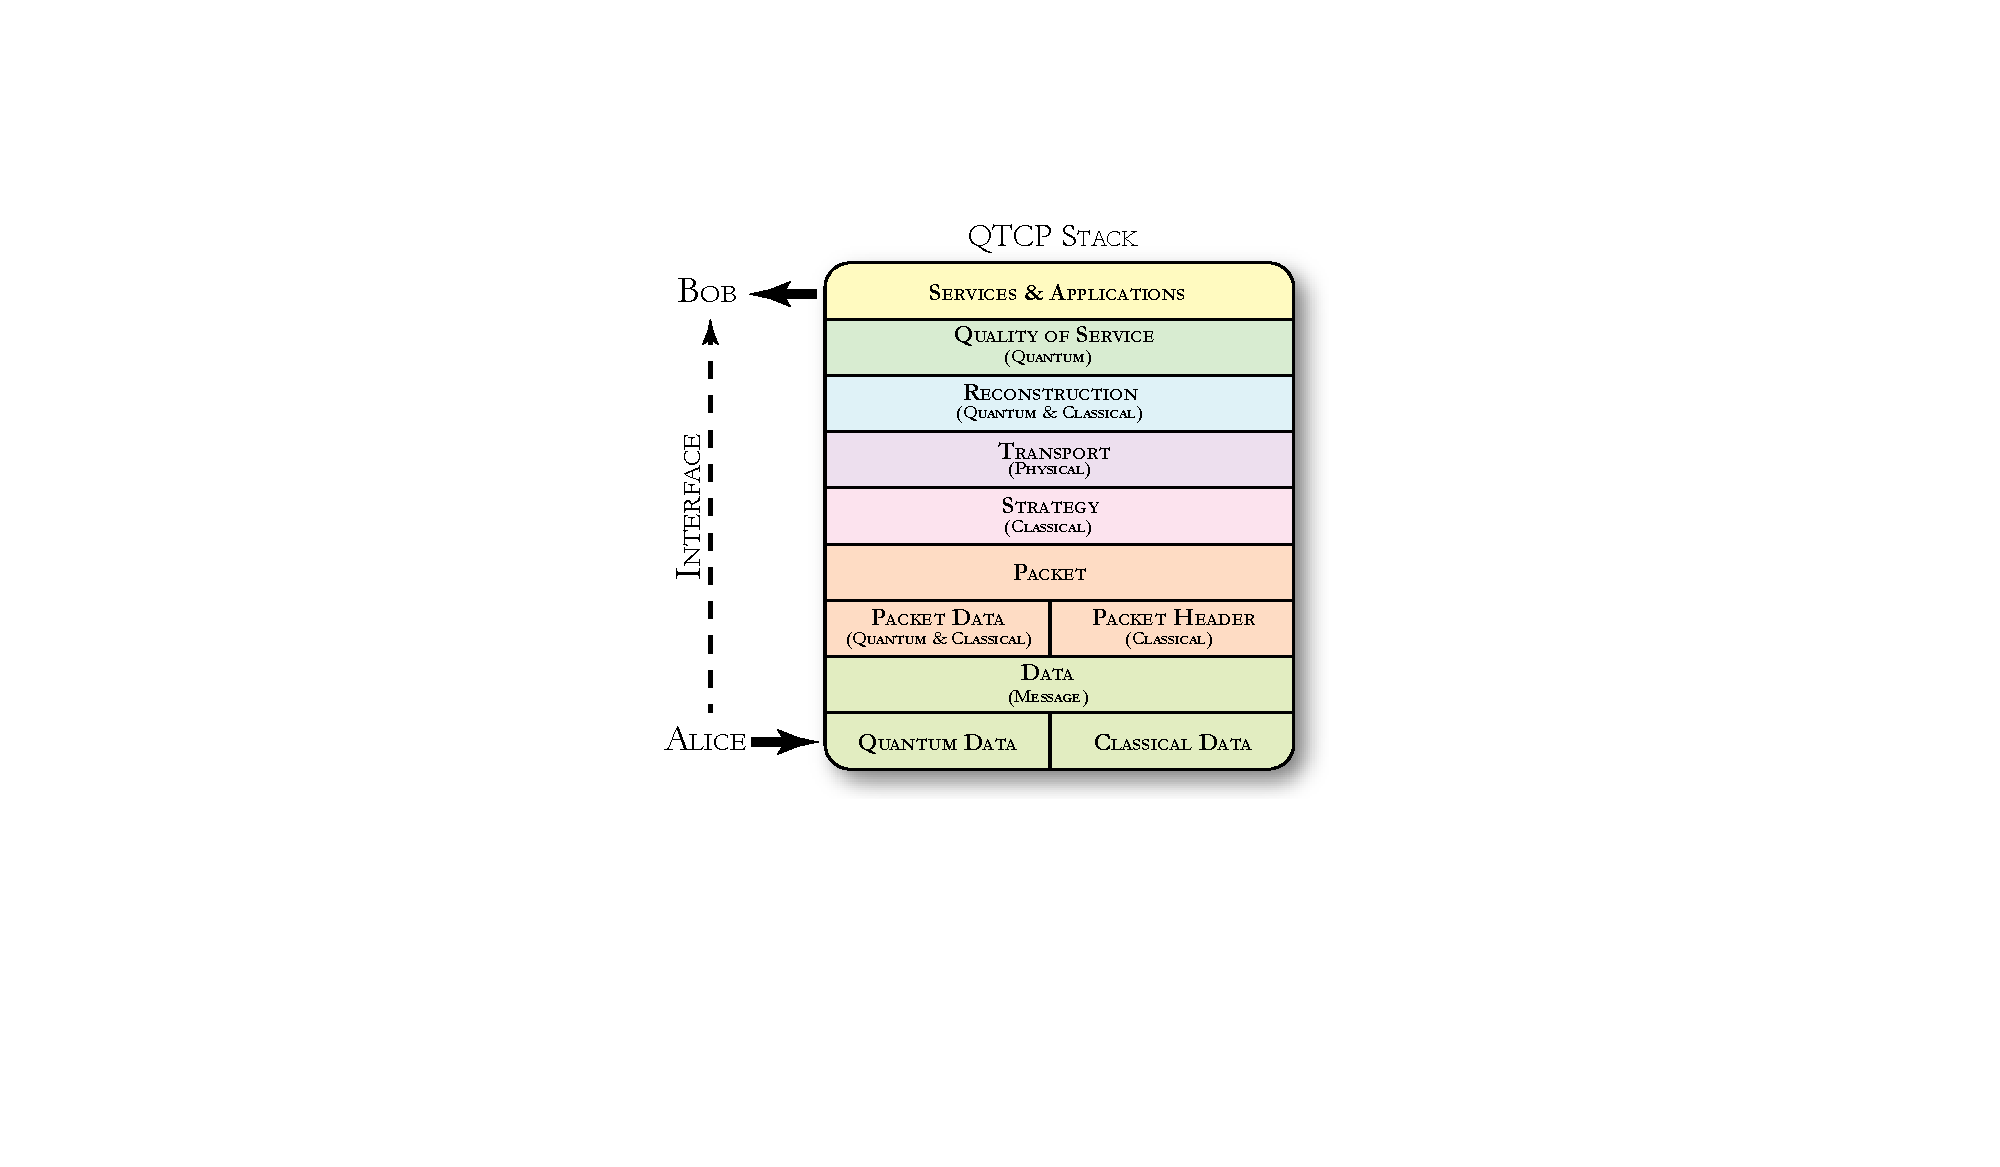
\includegraphics[clip=true, width=0.475\textwidth]{stack}
\else
\includegraphics[clip=true, width=0.6\textwidth]{stack}
\fi
\captionspacefig \caption{Protocol stack for QTCP. The protocol stack mediates communication of quantum data from Alice to Bob using the shown layers of abstraction. The end goal is to provide Bob a virtual interface to Alice's transmitted data, while remaining oblivious to the underlying protocol.} \label{fig:stack}\index{QTCP protocol stack}
\end{figure}

Next we describe the operation of these layers in detail.

%
% Data (Message)
%

\subsubsection{Data (Message)} \index{Data (message) layer} \label{sec:data_message_layer}

At the lowest level of the protocol we have the raw \textsc{Data} Alice wishes to communicate to Bob. \textsc{Data} is allowed to comprise both \textsc{Quantum Data} and \textsc{Classical Data} components, and may contain one or the other, or both.

%
% Quantum Data
%

\paragraph{Quantum data} \index{Quantum data layer}

\textsc{Quantum Data} is allowed to be an arbitrary quantum state. It could be a pure or mixed state, of arbitrary (but predetermined) dimension, or even a subsystem of a larger external state (i.e entangled with another system). We stress that it needn't be expressed using a conventional qubit representation, in the way digital data is necessarily represented using bits. Keep in mind that the quantum internet isn't just there to communicate qubit data streams. Rather, it is intended to act as generally as possible, such that essentially arbitrary \textit{quantum assets}\index{Quantum assets} can be exchanged. These needn't be restricted to any particular type of encoding, such as those discussed in Sec.~\ref{sec:opt_enc_of_qi}. For example, in addition to something `standard' like polarisation-encoded qubits in single photons, one network user might like to share an exotic CV state of light, like a cat state, with his mate whose cat died. Indeed, multiple types of state encoding might be encapsulated within a single \textsc{Packet}. The QTCP acts only as an abstract interface for quantum networking, but is completely blind as to what the underlying data in the network is. QTCP is only concerned with getting that state from Alice to Bob.

%
% Classical Data
%

\paragraph{Classical data} \index{Classical data layer}

\textsc{Classical Data} is a purely classical state with no coherence (i.e a diagonal density matrix), which may be represented as a classical bit-string. We very intentionally segregate the \textsc{Classical} and \textsc{Quantum} components of \textsc{Data}, since the classical network is expected to be cheaper and more reliable than the quantum network operating in parallel to it. The \textsc{Classical Data} could, for example, provide nodes with classical instructions on what quantum computations to perform on the \textsc{Quantum Data}.

%
% Packet
%

\subsubsection{Packet} \label{sec:packet_layer} \index{Packet!Layer}

\textsc{Data} is transmitted as \textsc{Packets}, much in the same way as conventional TCP. The \textsc{Data} is decomposed into three components: \textsc{Quantum Data}, \textsc{Classical Data}, and \textsc{Packet Header}.

We can express the state of an entire \textsc{Packet} as,
\begin{align}
\hat\rho_\mathrm{packet}(i) = \hat\rho_\mathrm{quantum}(i) \oplus \hat\rho_\mathrm{classical}(i) \oplus \hat\rho_\mathrm{header}(i),
\end{align}
where $i$ denotes the $i$th packet. Here $\hat\rho_\mathrm{quantum}$ ($\hat\rho_\mathrm{classical}$) is a block of \textsc{Quantum Block Size} qubits (\textsc{Classical Block Size} bits) taken from the user's \textsc{Quantum Data} (\textsc{Classical Data}), while $\hat\rho_\mathrm{header}$ is the \textsc{Packet's} classical \textsc{Packet Header}. As discussed earlier, since $\hat\rho_\mathrm{quantum}$ is quantum, and $\hat\rho_\mathrm{classical}$ and $\hat\rho_\mathrm{header}$ are classical, they needn't be transmitted together over the same quantum network. Instead all \textsc{Classical Data} and \textsc{Packet Header} could be transmitted over a classical network operating in parallel to and synchronised with the quantum network, which carries the \textsc{Quantum Data}.

Note that while one can always measure classical data without disturbance, this is not the case with quantum data, where measurements cause wave-function collapse. Thus, while Alice is always able to know $\hat\rho_\mathrm{classical}$ and $\hat\rho_\mathrm{header}$, she may or may not know $\hat\rho_\mathrm{quantum}$. Clearly if she prepared the state herself, she would (hopefully) know what she was doing. But in general, quantum networks could be used for far less trivial networking, where Alice is, for example, an intermediary in a distributed quantum computation. In this instance, Alice is unlikely to know what her \textsc{Quantum Data} is.

%
% Packet Data
%

\paragraph{Packet data} \index{Packet!Data layer}

Comprises blocks of both \textsc{Quantum Data} and \textsc{Classical Data}, of sizes \textsc{Quantum Block Size} and \textsc{Classical Block Size} respectively. \textsc{Packet Data} requires that \textsc{Data} be decomposed into distinct subsystems which are independently transmitted by QTCP. For easy of exposition, we will restrict ourselves to the case where the \textsc{Data} is encoded into a stream of qubits (\textsc{Quantum Data}) and bits (\textsc{Classical Data}). But of course other encodings could be used. Also bear in mind that any quantum (classical) information can be encoded into qubits (bits), and once represented as such, the decomposition of \textsc{Data} into \textsc{Packets} arises very naturally and intuitively. The \textsc{Packet's} \textsc{Quantum Data} is what is transmitted via the quantum channels, while the \textsc{Classical Data} is communicated via classical channels.

%
% Packet Header
%

\paragraph{Packet header} \label{sec:packet_header} \index{Packet!Header layer}

\textsc{Packet Header} is purely classical and needn't be transmitted over the costly quantum network, instead being transmitted over a complementary classical network, running in parallel to, and synchronised with the quantum network. \textsc{Packet Header} contains no information content from \textsc{Data}, instead comprising only metadata relevant to the higher levels of the protocol stack. In particular, \textsc{Packet Header} contains the following fields:
\begin{itemize}
    \item \textsc{Header Size}\index{Header size}: The number of bits in the \textsc{Packet Header}.
    \item \textsc{Message ID}\index{Message ID}: A unique identifier for the complete message to which this \textsc{Packet} belongs. This field mitigates ambiguity as to which \textsc{Message} this packet belongs when performing \textsc{Reconstruction}.
    \item \textsc{Lifetime}\index{Lifetime}: How long the \textsc{Packet} has been in existence for, i.e since it was initially sent by the \textsc{Sender}. This is used by strategies to prevent collisions.
    \item \textsc{Sender}\index{Sender}: A unique node identifier for the sender (Alice).
    \item \textsc{Recipient}\index{Recipient}: A unique node identifier for the recipient (Bob).
    \item \textsc{Order}\index{Order}: To which block taken from \textsc{Data} does this \textsc{Packet Data} belong? This is extremely important in networks where \textsc{Packets} may arrive out of order. The \textsc{Order} field forms the basis for the \textsc{Reconstruction} layer.
    \item \textsc{Quantum Block Size}\index{Quantum block size}: The number of qubits contained in the \textsc{Quantum} component of \textsc{Packet Data}. This is important for the \textsc{Reconstruction} layer.
    \item \textsc{Classical Block Size}\index{Classical block size}: The number of bits contained in the \textsc{Classical} component of \textsc{Packet Data}, also important for the \textsc{Reconstruction} layer.
    \item \textsc{Routing Queue}\index{Routing!Queues}: A first in, first out (FIFO) queue of node identifiers, tracing out the entire route for the \textsc{Packet} to follow, in chronological order from the next node to visit all the way to the \textsc{Recipient}.
    \item \textsc{Costs}\index{Costs}: A tuple characterising all the accumulated costs of the \textsc{Packet} at the current stage in the route. These are treated as accumulators that are incremented appropriately after each step, since costs are additive.
    \item \textsc{Attributes}\index{Attributes}: A tuple characterising all the non-\textsc{Cost} properties associated with the \textsc{Packet}. Examples include: the \textsc{Priority} of routing a \textsc{Packet} to its destination; suggesting a preferred routing \textsc{Strategy}; or, indicating whether or not a \textsc{Resend Until Success} protocol may be applied to this \textsc{Packet}.
    \item \textsc{Padding}\index{Padding}: Null data to pad the joint \textsc{Classical Packet Data} and \textsc{Packet Header} fields to be of the same length as the \textsc{Quantum Packet Data}. This ensures that the components of the \textsc{Packet} traversing the quantum and classical channels remain in perfect tandem -- bit for qubit. In Sec.~\ref{sec:transport} we show that this facilitates collision detection without the need to measure quantum states.
    \item \textsc{Checksum}\index{Checksums}: A regular checksum of the entire \textsc{Classical} component of the \textsc{Packet}, including both \textsc{Classical Packet Data} and \textsc{Packet Header}. This also forms a part of the collision detection protocol.
\end{itemize}

One might question why \textsc{Packet Headers} tally accumulated costs when we ought to already know all the costs, since these were employed by the algorithm for choosing strategies in the first case. In the ideal case where all strategies are determined \textit{a priori} and are implemented as intended, this is certainly valid. However, for generality we retain this option since more realistic networks may require dynamically updating strategies during the course of propagation, in which case dynamically tallying costs is appropriate.

%
% Strategy
%

\subsubsection{Strategy} \label{sec:intro_strat} \index{Strategy!Layer}

Based on the \textsc{Packet Headers} of all users sharing the network, choose routing strategies to optimise cost metrics. The notion of strategies is introduced in Sec.~\ref{sec:strat_opt}, and a detailed discussion of example strategies is presented in Sec.~\ref{sec:strategies}.

Once routings have been determined for all \textsc{Packets}, the \textsc{Routing Queues} in their \textsc{Packet Headers} are initialised accordingly by pushing the sequence of node identifiers tracing out the desired route.

In the case of dynamic, time-dependent strategies, which can be updated within the duration of transmissions, the \textsc{Routing Queues} may need to be updated. A change in a \textsc{Packet's} route simply requires flushing the queue and pushing new node identifiers for each of the nodes in the new route, in chronological order.

The \textsc{Strategy} layer is responsible for evaluating the net cost function $f_\mathrm{cost}$ from Eq.~(\ref{eq:net_cost_R}), which accounts for both \textsc{Costs} and \textsc{Attributes} to calculate a single effective cost measure that may be employed in routing decisions.

%
% Transport
%

\subsubsection{Transport} \label{sec:transport} \index{Transport layer}

The \textsc{Transport} layer is responsible for actual routing at the physical level, making direct decisions as to what to do with a \textsc{Packet} at each step, based upon the metadata contained in \textsc{Packet Header}, most notably the \textsc{Routing Queue}, which specifies the full route a \textsc{Packet} is destined to follow. It is also responsible for keeping track of costs that accumulate over their route.

Additionally, the \textsc{Transport} layer is responsible for collision detection, whereby multiple packets being transmitted simultaneously over a network interfere with one another, corrupting the data. In classical networking, collision detection is straightforward using checksums. But the usual classical approach breaks down in the quantum setting. In Sec.~\ref{sec:collision} we discuss in detail collision detection in QTCP.

The pseudo-code algorithm implemented by the \textsc{Transport} layer, including collision detection, is shown in Alg.~\ref{alg:transport_alg}.

\startalgtable
\begin{table}[!htbp]
\begin{mdframed}[innertopmargin=3pt, innerbottommargin=3pt, nobreak]
\texttt{
function Transport(Packet):
\begin{enumerate}
    \item nextNode = Packet.RoutingQueue.Pop()
    \item Packet.PhysicallySendTo(nextNode)
    \item Packet.WaitUntilArrivesAt(nextNode)
    \item checksum = Hash(Packet.Header + Packet.ClassicalData)
    \item if(checksum $\neq$ Packet.Header.Checksum) \{
    \setlength{\itemindent}{0.2in}
    \item Packet.Sender.Notify(\textsc{Failure})
    \item Packet.Recipient.Notify(\textsc{Failure})
    \item Packet.Discard()
    \item $\Box$
        \setlength{\itemindent}{0in}
\item \}
    \item Packet.Costs += IncomingLink.Costs
    \item Packet.Attributes.Update()
    \item if(Packet.RoutingQueue.Length = 0) \{
    \setlength{\itemindent}{0.2in}
    \item Return(Packet)
        \setlength{\itemindent}{0in}
    \item \}
    \setlength{\itemindent}{0in}
    \item $\Box$
\end{enumerate}}
\end{mdframed}
\captionspacealg \caption{Algorithm implemented by the \textsc{Transport} layer of QTCP for each \textsc{Packet}. The \texttt{Attributes.Update()} function is left undefined. This is where arbitrary \textsc{Attribute} dynamics may take place.} \label{alg:transport_alg}
\end{table}

%
% Reconstruction
%

\subsubsection{Reconstruction} \index{Reconstruction layer} \label{sec:reconstruction_layer}

The \textsc{Reconstruction} layer only serves one purpose -- to chronologically reorder the received \textsc{Packets} based on the \textsc{Order} field in their \textsc{Packet Headers}. This stage is only performed by Bob -- the final recipient -- and not at any intermediate stage. In general this will require Bob to have a quantum memory, able to hold all \textsc{Packet Data} for a sufficient duration as to enable an arbitrary permutation of \textsc{Packets} to be applied, reproducing the correct chronological order. The algorithm for this is shown in Alg.~\ref{alg:reconstruction}.

\begin{table}[!htbp]
\begin{mdframed}[innertopmargin=3pt, innerbottommargin=3pt, nobreak]
\texttt{
function Reconstruction(Packets):
\begin{enumerate}
    \item Packets.WaitUntilAllReceived()
    \item message =\\ 
    Packets.SortByOrderAscending().data
    \item Packets.Receiver.Notify(message)
     \item $\Box$
\end{enumerate}}
\end{mdframed}
\captionspacealg \caption{The goal of the \textsc{Reconstruction} layer, is to take a collection of received \textsc{Packets} and reassemble them into the \textsc{Message}.} \label{alg:reconstruction}
\end{table}

%
% Quality of Service (QoS)
%

\subsubsection{Quality of service} \label{sec:QOS} \index{Quality of service (QoS)!Layer}

In classical networking theory, error detection and correction is an important element of networking protocols. Communication links may be unreliable, or subject to external noise, which users must be able to detect so as to guarantee the quality of their data.

Classically, error detection is typically performed using checksums (hash functions), which generate a short digest of a packet's data that can be recalculated upon arrival to verify integrity. The checksum can be included in the header component of each packet, allowing the remainder of the protocol to remain unchanged.

In the quantum context the elegant notion of checksums is complicated by the fact that calculating a hash function of a quantum state would necessarily entangle the state with the output hash. This would have the undesired effect of causing measurement of the checksum to collapse the quantum state of the data, thereby altering it in an uncontrollable way.

As an alternative to checksums, we could borrow the notion of quantum error correction (QEC)\index{Quantum error correction (QEC)} and fault-tolerance\index{Fault-tolerance} from quantum computing theory \cite{???}. Here we encode a quantum state into a (polynomially) larger Hilbert space. \textit{Syndrome measurements}\index{Syndromes!Measurements} on some of the states in this larger space allow us to both detect and correct universal error models, such as depolarisation or dephasing, provided that error rates are within the fault-tolerance threshold of the code being employed.

Thus, enforcing QoS in fundamentally different for quantum data packets than for classical ones, requiring entirely different techniques. Given how large a field this has become in its own right, we dedicate Sec.~\ref{sec:QOS_chap} entirely to protocols suited to the implementation of quantum QoS requirements in quantum networks.

%
% Services & Applications
%

\subsubsection{Services \& applications} \index{Services \& applications layer} \label{sec:services_apps}

Having communicated all the \textsc{Packet Data} from Alice to Bob, performed \textsc{Reconstruction}, and applied \textsc{QoS} protocols, Bob ought to have $\hat\rho_\mathrm{data}$ to a good approximation. The quality of Bob's received state can be inferred directly from the \textsc{Costs} vector contained in the \textsc{Packet Headers}. The final state and its associated quality metrics (\textsc{Costs} and QEC outcomes) may then be provided to Bob as a software interface for end use.
\sketch{sketch_37}

\latinquote{Divide et impera.}

%
% Collision Handling & Classical Errors
%

\subsection{Collision handling \& classical errors} \label{sec:collision} \index{Collision handling} \index{Classical errors}

In classical networking, protocols such as Ethernet allow users to simply broadcast data at their leisure and rely on \textit{collision detection} to detect when the broadcasts of multiple users have interfered, signalling that both users ought to retransmit following backoff, to minimise the chances of another collision occurring. While this \textsc{Resend Until Success} approach has certainly proven to be effective in classical networking, in a quantum setting the rules of the game are entirely different.

First, collision detection necessarily requires measuring a communications channel to test whether data has been corrupted. Classical networks typically do this by transmitting a checksum with the data, which is recalculated upon arrival for comparison. This raises the obvious problem that quantum measurements are destructive, which means that testing the integrity of our data destroys it in the process -- the last feature we'd like our network to exhibit! However, to overcome this, in Sec.~\ref{sec:transport} we describe a protocol based on the dual classical/quantum network that allows collision detection without measuring quantum states.

Second, collision detection is not always even allowed at all. If one of Alice's packets was entangled with another (i.e she was communicating an entangled system, where the different subsystems resided in different packets), she would not be able to simply retransmit an identical copy of the corrupted packet, since the entanglement with the other system would have been lost and there are no local operations she can do to recover it.

Alternately, Alice might be a part of a distributed computation, where she didn't prepare the data in the first place. In this instance, the no-cloning theorem implies that she cannot, in general, learn what the quantum state was, and therefore would be unable to make a second transmission attempt.

From Alice's point of view, \textsc{Resend Until Success} would clearly work if she was preparing a known state, separable from the other packets. However, collisions on the network caused by her reckless resending would likely corrupt the communications between other parties, leaving them rather ticked off at her.

There are therefore two main approaches to dealing with collisions. First, central planning of all routing could be employed, precisely scheduling all routes \textit{a priori} so as to entirely eliminate any possibility for collisions. Second, if all users in the network were communicating data where packet loss could be tolerated, they could all mutually agree to use the \textsc{Resend Until Success} protocol. This would not require a central authority, and be highly desirable for ad hoc networks. It is important to stress, however, that the latter requires unanimity amongst network participants to function, and the restriction to known, separable states is a major limitation that would prohibit many important uses for quantum networks, such as distributed quantum computation. However, both these approaches are entirely valid in their appropriate context.

In classical TCP all components of data packets are classical and are kept together throughout every stage of transmission. In the quantum case we will instead have a mixture of both quantum and classical data. As mentioned, we will assume that classical communication and computation resources `come for free' (or are at least cheap compared to quantum resources), so there will be a clear disambiguation as to what data is quantum or classical within packets.

As discussed, quantum collision detection is complicated by the fact that measuring quantum data to determine whether it has been corrupted disturbs the quantum state. We address this problem by taking advantage of the duality of the quantum/classical network, discussed in Sec.~\ref{sec:quant_net}. Because the quantum and classical components of the \textsc{Packets} are synchronised and of equal length (thanks to the \textsc{Padding} field of the \textsc{Packet Header}), and because the same applies to all other \textsc{Packets} on the network, a collision in the quantum data necessarily implies a collision in the classical data, and vice versa. Therefore, by applying regular classical collision detection techniques based on checksums (recall \textsc{Packet Header} contains a \textsc{Checksum} field), we can infer collisions in quantum data without actually measuring it. We refer to this as \textit{indirect collision detection}\index{Indirect collision detection}. This guarantees us the ability to detect when a collision has occurred, in which case both quantum \textit{and} classical data are corrupted, or has not occurred, in which case both quantum and classical data are uncorrupted and the quantum data remains unmeasured. Collision detection is incorporated into the pseudo-code implementation of the \textsc{Transport} layer shown in Alg.~\ref{alg:transport_alg}.

This algorithm could, depending upon implementation, be executed locally on the node currently hosting the \textsc{Packet}, or it could be delegated to a central authority, but with the overhead of additional classical communication.

In instances where corruption or loss of packets cannot be tolerated, a more proactive approach may be applied. To preempt the risk of packet collision, one could introduce \textit{probe packets}\index{Probe packets} -- packets containing only classical data, that query a route ahead to negotiate channel usage for the following proper packet, thereby avoiding collisions. Of course, if an upcoming node is unable to guarantee channel capacity immediately, the packet may need to be stored in quantum memory until the channel is available. Thus, it is important to accommodate for this by ensuring that quantum memory is available in nodes preceding links/nodes where collisions are not guaranteed to be mitigated immediately. Quantum memory will be discussed in Sec.~\ref{sec:memory}.
\sketch{sketch_15}

\latinquote{Esse est percipi.}

%
% Multi-Packet Operations
%

\subsection{Multi-packet operations} \index{Multi-packet operations}

\comment{To do}

Thus far we have considered nodes which implement single-packet operations. However, many real-world quantum protocols (to be presented in Part.~\ref{part:protocols}) will require multi-packet operations, which must be carefully combined in some well-defined way. For example, for state teleportation (Sec.~\ref{sec:teleport}) we must combine a data packet with half of a Bell pair (Sec.~\ref{sec:bell_state_res}). For entanglement swapping (Sec.~\ref{sec:swapping}) -- the essential component in quantum repeater networks (Sec.~\ref{sec:rep_net}) -- two halves of distinct Bell pairs undergo a joint entangling measurement.

To accommodate such multi-packet operations, we must add some modifications to the QTCP protocol to handle:
\begin{itemize}
	\item Packet synchronisation\index{Packet!Synchronisation}: multiple packets subject to joint operations must be time-synchronised upon implementation of the joint operation. This might involve holding one packet in a quantum memory whilst waiting upon another. Thus, the time required to implement the joint operation is bottlenecked by the packet slowest to arrive.
	\item Bookkeeping of costs and attributes\index{Combining costs \& attributes}: when multiple packets are combined under some operation, how do error costs and attributes accumulate?
	\item Partner packet tracking\index{Partner packet tracking}: packets must keep track of the partner packets with which they are intended to undergo joint operations with. This may be achieved with the addition of \textsc{Partners} fields in the packet headers, containing an array of their \textsc{Message ID}'s.
	\item Operation signalling\index{Operation signalling}: the recipient node of multiple packets undergoing a joint operation must be informed as to what joint operations should be applied. This may be implemented via the addition of a \textsc{What Operation} field to the header.
\end{itemize}

At a high level, these may be implemented in the \textsc{Transport} layer as outlined in Alg.~\ref{alg:trans_multi_packet}, where we have intentionally left the functions for combining costs and attributes unspecified. In many instances, the \texttt{CombineCosts()} function could be as simple as a summation of its arguments.

\begin{table}[!htbp]
\begin{mdframed}[innertopmargin=3pt, innerbottommargin=3pt, nobreak]
\texttt{
function Transport.MultiPacketOperation(packets):
\begin{enumerate}
	\item for(packet$\in$packets) \{
	\setlength{\itemindent}{0.2in}
	\item packet.WaitFor()
	\item packet.HoldInMemory()
	\setlength{\itemindent}{0in}
	\item \}
    \item output = SomeOperation(packets.WhatOperation, packets)
    \item if(output.OperationSuccess = true) \{
	\setlength{\itemindent}{0.2in}
    \item packets.Sender.Notify(\textsc{Success})
    \item output.Costs = CombineCosts(packets.Costs)
    \item output.Attributes = \\
    CombineAttributes(packets.Attributes)
    \item return(output)
	\setlength{\itemindent}{0in}
    \item \} else \{
	\setlength{\itemindent}{0.2in}
    \item packets.Sender.Notify(\textsc{Failure})
  	\setlength{\itemindent}{0in}
    \item \}
    \item $\Box$
\end{enumerate}}
\end{mdframed}
\captionspacealg \caption{High-level structure of transport layer implementation of multi-packet operations.}\index{Multi-packet operations} \label{alg:trans_multi_packet}
\end{table}

%
% Combining Costs & Attributes
%

\subsubsection{Combining costs \& attributes} \index{Combining costs \& attributes}

Let us now turn our attention to the details of how the \texttt{CombineCosts()} and \texttt{CombineAttributes()} functions might be implemented. In Sec.~\ref{sec:quantum_meas_cost} we presented a number of examples of prominent costs and attributes that might arise in quantum networks.

To illustrate the basic idea behind this, we now turn our attention to several examples for combining costs and attributes. Some details may vary between specific quantum protocols, although the following typically apply in most general cases.

These ideas logically extend all the way from simple state teleportation to more complicated multi-packet protocols, all the way up to fully distributed quantum computations involving large numbers of qubits and nodes (Sec.~\ref{sec:dist_QC}).

\comment{To do}

%
% Efficiency
%

\paragraph{Efficiency} \index{Loss!Channel}

\begin{table}[!htbp]
\begin{mdframed}[innertopmargin=3pt, innerbottommargin=3pt, nobreak]
\texttt{
function CombineCosts.Efficiency(packets):
\begin{enumerate}
	\item costs = packets.Costs.Efficiency
	\item netCost = sum(costs)
	\item return(netCost)
    \item $\Box$
\end{enumerate}}
\end{mdframed}
\captionspacealg \caption{Algorithm for combining efficiency metrics in a multi-packet protocol.} \label{alg:combine_eff}
\end{table}

\comment{To do}

%
% Decoherence
%

\paragraph{Decoherence} \index{Decoherence}

\begin{table}[!htbp]
\begin{mdframed}[innertopmargin=3pt, innerbottommargin=3pt, nobreak]
\texttt{
function CombineCosts.Decoherence(packets):
\begin{enumerate}
	\item maxDecoherence = \\
    max(packets.Costs.Decoherence)
    \item return(maxDecoherence)
    \item $\Box$
\end{enumerate}}
\end{mdframed}
\captionspacealg \caption{Transport layer algorithm for combining decoherence rates in a multi-packet protocol.} \label{alg:combine_lat}
\end{table}

\comment{To do}

%
% Latency
%

\paragraph{Latency} \index{Latency}

In state teleportation there are three channels side-by-side, each exhibiting their own distinct latencies. However, as they are in parallel, the net latency will not be the accumulation of the individual latencies, but rather determined by the largest of those three latencies. That is, the slowest qubit acts as a bottleneck. This is shown in Alg.~\ref{alg:combine_lat}.

\begin{table}[!htbp]
\begin{mdframed}[innertopmargin=3pt, innerbottommargin=3pt, nobreak]
\texttt{
function CombineCosts.Latency(packets):
\begin{enumerate}
	\item maxLatency = max(packets.Costs.Latency)
    \item return(maxLatency)
    \item $\Box$
\end{enumerate}}
\end{mdframed}
\captionspacealg \caption{Transport layer algorithm for combining latencies in a multi-packet protocol.} \label{alg:combine_lat}
\end{table}

\comment{To do}

%
% Dollars
%

\paragraph{Dollars} \index{Dollar cost}

Dollars are perhaps the simplest of costs to account for, as they are simply additive -- the dollar cost of a protocol is the sum of the dollar cost of each component within it. This is shown in Alg.~\ref{alg:combine_dol}.

\begin{table}[!htbp]
\begin{mdframed}[innertopmargin=3pt, innerbottommargin=3pt, nobreak]
\texttt{
function CombineCosts.Dollars(packets):
\begin{enumerate}
	\item costs = packets.Costs.Dollars
	\item netCost = sum(costs)
	\item return(netCost)
	\item $\Box$
\end{enumerate}}
\end{mdframed}
\captionspacealg \caption{Transport layer algorithm for combining dollar costs in packet teleportation.} \label{alg:combine_dol}
\end{table}

\comment{To do}
\sketch{sketch_17}

\latinquote{Capax infiniti.}

%
% Extensibility of QTCP
%

\subsection{Extensibility of QTCP}\index{Extensibility of QTCP} \label{sec:c_vs_a}

In Sec.~\ref{sec:costs} we introduced the notion of the \textit{costs} and \textit{attributes} of links in a classical network, and in Sec.~\ref{sec:quantum_meas_cost} generalised these notions to the quantum case. In Sec.~\ref{sec:packet_header} we described the header format for quantum packets.

The \textsc{Costs} and \textsc{Attributes} fields within the \textsc{Header} are very powerful data structures, implemented as ordered sets of arbitrary dimension, comprising arbitrary data fields. The intention here is to allow QTCP to be extensible into the future, with the addition of new data structures into the protocol. These can be custom designed to, in conjunction with appropriate routing strategies and cost functions, influence the operation of QTCP completely arbitrarily, and easily implement entirely different quantum networking paradigms than presented here.

\textsc{Costs} naturally capture characteristics of the network that accumulate additively along routes, whereas \textsc{Attributes} capture any other characteristics that aren't additive. A network needn't have both costs \textit{and} attributes. It may have one or the other, or both, but not neither, since there must be some measure by which to judge routes.

\comment{To do!}
\sketch{sketch_18}

\latinquote{Cedere nescio.}

%
% Scalability of QTCP
%

\subsection{Scalability of QTCP}\index{Scalability of QTCP}

\comment{To do}

\comment{Discussion of how QTCP protocol/policies might be designed to change with scale. E.g for a small LAN the policies/metrics/attributes might be completely different than for an intercontinental uplink. Discuss how this scalability might be implemented, with examples.}
\sketch{sketch_41}

\latinquote{Citius altius forties.}

%
% Quality of Service
%

\section{Quality of service (QoS)}\index{Quantum error correction (QEC)}\index{Quality of service}\label{sec:QOS_chap}

As discussed previously in Sec.~\ref{sec:QOS}\index{Quality of service}, quality of service is a major consideration in any quantum network. If we are transmitting quantum states over a quantum channel, there will inevitably be deterioration in the form of decoherence, loss, and other undesirable effects we wish to mitigate. In this section we review some of the essential quantum error correction (QEC) techniques that can be used to achieve this.

Different error correcting codes have different error correcting power, and different resource overheads, which must be taken into consideration. The appropriate choice of code will largely be determined by the final \textsc{Services \& Applications} layer. For some simple quantum communications protocols, simple error correction (or even no error correction) may suffice. A full-fledged quantum computation on the other hand will require error rates within a fault-tolerance threshold\index{Fault-tolerance threshold}.

%
% Entanglement Purification
%

\subsection{Entanglement purification}\index{Entanglement purification}

\comment{To do - move from protocols section. Here do circuit description. Leave optical implementation in protocols section.}

%
% 3-Qubit Code
%

\subsection{3-qubit code}\index{3-qubit code}

The first described QEC\index{Quantum error correction (QEC)} code was the 3-qubit code\index{3-qubit code} by \cite{bib:Shor95} for redundantly encoding a single logical qubit into three encoded qubits, allowing the detection and correction of at most a single bit-flip error between the encoded qubits. Measurement of the three ancillary qubits yields a \textit{syndrome}\index{Syndrome}, which identifies where the error took place, allowing it to be subsequently corrected with feedforward. This protocol is shown in Alg.~\ref{alg:three_QEC}.

By switching into a Hadamard-rotated basis, the same code could equivalently correct against at most a single phase-flip error (since \mbox{$\hat{H}\hat{X}\hat{H}=\hat{Z}$}).

\begin{table}[!htb]
\fbox{\parbox{0.965\columnwidth}{\texttt{
function ThreeQubitCode($\ket\psi$):
\begin{enumerate}
\item Using two CNOT gates, redundantly encode the logical single-qubit state,
\begin{align}
\ket\psi=\alpha\ket{0}+\beta\ket{1},
\end{align}
into the 3-qubit state,
\begin{align}
\ket\psi_R &= \hat{\text{CNOT}}_{1,2}\hat{\text{CNOT}}_{1,3}\ket\psi\ket{00} \nonumber \\
&= \alpha\ket{000}+\beta\ket{111}.
\end{align}
\item Independently apply bit-flip channels $\mathcal{E}_X$ to each of the three encoded qubits.
\item If exactly one bit-flip operation was applied in total, the three possible erroneous encoded states are,
\begin{align}
\ket\psi_1 &= \hat{X}_1 \ket\psi_R = \alpha\ket{001}+\beta\ket{110}, \nonumber \\
\ket\psi_2 &= \hat{X}_2 \ket\psi_R = \alpha\ket{010}+\beta\ket{101}, \nonumber \\
\ket\psi_3 &= \hat{X}_3 \ket\psi_R = \alpha\ket{100}+\beta\ket{011}.
\end{align}
\item Determine the parity of each of the three pairs of encoded qubits.
\item Assuming at most a single bit-flip operation has occurred on the encoded state, the three parity outcomes uniquely determine which encoded qubit the bit-flip was applied to.
\item Apply classically-controlled bit-flip recovery operations, $\mathcal{R}$, to correct the encoded state, recovering $\ket\psi_R$.
\item Apply the inverse of the encoding operation to recover $\ket\psi$.
\item $\Box$
\end{enumerate}}
\begin{align}
\Qcircuit @C=1.3em @R=.6em {
  & \lstick{\ket{\psi}} & \ctrl{2} & \gate{\mathcal{E}_X}  & \qw & \qw              & \ctrl{3}  & \qw       & \ctrl{4} & \qw & \multigate{2}{\ \mathcal{R}\ } & \qw \\
  & \lstick{\ket{0}}    & \targ    & \gate{\mathcal{E}_X}  & \qw & \qw              & \ctrl{2}  & \ctrl{2}  & \qw      & \qw & \ghost{\ \mathcal{R}\ } \qw & \qw \\
  & \lstick{\ket{0}}    & \targ    & \gate{\mathcal{E}_X}  & \qw & \qw              & \qw       & \ctrl{2}  & \ctrl{3} & \qw & \ghost{\ \mathcal{R}\ } \qw & \qw \\
  &          &          &          & & \lstick{\ket{0}} & \targ \qw & \qw       & \qw      & \meter & \control \cw \cwx \\
  &          &          &          & & \lstick{\ket{0}} & \qw       & \targ \qw & \qw      & \meter & \control \cw \cwx \\
  &          &          &          & & \lstick{\ket{0}} & \qw       & \qw       & \targ    & \meter & \control \cw \cwx
} \nonumber
\end{align}
}}
\caption{3-qubit code for protecting against at most a single logical bit-flip error. The doubly-controlled CNOT gates represent parity measurements, \mbox{$n_3=n_1\oplus n_2$}, where $n_i$ represents the value of the $i$th qubit. In a Hadamard-rotated basis, the same circuit may be employed to protect against a single phase-flip error. And by concatenating the two we obtain a 9-qubit code protecting against a single depolarising error (i.e joint bit-flip/phase-flip), which is a universal single-qubit error model.} \label{alg:three_QEC}
\end{table}

%
% 9-Qubit Code
%

\subsection{9-qubit code}\index{9-qubit code}

By taking two instances of the 3-qubit code, one implementing bit-flip correction and the other implementing phase-flip correction, and concatenating them, we can define a 9-qubit code, which protects against at most a single bit-flip and a single phase-flip. Joint protection against both the bit-flip and phase-flip operators ($\hat{X}$ and $\hat{Z}$) in turn allows error correction against a single depolarising error, the most general type of logical error, which completely destroys a single qubit.

This is the simplest construction of a code which protects against a single depolarising event. But it is not the most efficient, and numerous more resource-savvy codes for protecting against Pauli errors exist, such as Steane's 7-qubit code\index{Steane code} \cite{SteaneCode}.

%
% Stabiliser Codes
%

\subsection{Stabiliser codes}\index{Stabiliser codes}

\comment{To do}

%
% Surface Codes
%

\subsection{Surface codes}\index{Surface codes}

\comment{These are a particular example of stabiliser codes with an elegant graphical interpretation}

\comment{Missing degree of freedom in stabilisers defines qubit. How does topology (genus) relate to number of logical qubits?}

If the intention is to perform quantum computations using cluster states shared over a network, QEC and fault-tolerance \textit{must} be taken into consideration, or catastrophic algorithmic failure will inevitably follow -- the cluster state model is no different from the circuit model in this respect. Fault-tolerance theory places hard thresholds on the amount of noise (typically depolarising errors and loss) qubits may be subject to in order for fault-tolerance to be possible and computations to succeed. This places strict QoS (Sec.~\ref{sec:QOS}) constraints on the network, which can be accommodated for using the usual depolarising and efficiency cost metrics when developing networking strategies and link performance requirements.

It has been shown that fault-tolerance is possible within the cluster state model \cite{bib:NielsenDawson04, bib:Dawson06} using variations of conventional QEC codes. However, more importantly, from cluster states certain \textit{topological QEC codes} \cite{???} can be readily constructed. This implements a form of QEC-encoded measurement-based quantum computing protocol, where the computation proceeds in a measurement-based fashion, but is `natively' fault-tolerant.

These codes have been shown to have very favourable fault-tolerance thresholds in terms of both depolarising noise and loss \cite{bib:StaceBarrettDohertyLoss, bib:BarrettStaceFT}, as well as frugal resource overhead compared to traditional concatenated codes. Additionally, loss- and gate-failure-tolerant codes, uniquely applicable to the cluster state model, have been described, with very favourable loss thresholds \cite{bib:Varnava05, bib:RalphHayes05, bib:Duan05}. 

Importantly, topological codes do not require joint measurements across the entire graph state, instead requiring only operations localised to small regions within the graph. Thanks to this, computation using such topological codes can remain distributed, without requiring the entire state to be held locally by a particular host, or requiring full access to the entire state by any particular user.

The most common topological code, which we will use here as an example, is the toric code\index{Toric code}, which resides on a lattice graph over the surface of a torus\footnote{As with cluster states, this graph needn't (but could) correspond to a network graph.}. As with cluster states (Sec.~\ref{sec:CSQC}), the toric code is most easily visualised in the stabiliser formalism\index{Stabiliser formalism}. Consider a rectangular sub-graph of the torus. We place a qubit on each edge (not vertex) of the graph. Now we define two sets of stabiliser operators: \textit{star} and \textit{plaquette} operators,
\begin{align} \index{Topological code stabilisers}\index{Star operator}\index{Plaquette operator}
	\hat{S}_\text{star}(v) &= \prod_{i\in e(v)} \hat{X}_i, \nonumber \\
	\hat{S}_\text{plaquette}(p) &= \prod_{i\in e(p)} \hat{Z}_i,
\end{align}
where $e(v)$ are the edges neighbouring vertex $v$, and $e(p)$ are the edges surrounding plaquette $p$. By definition, the toric code state, $\ket\psi_\text{toric}$, satisfies the stabiliser relations,
\begin{align}
	\hat{S}_\text{star}(v) \ket\psi_\text{toric} &= \ket\psi_\text{toric} \,\forall\, v, \nonumber \\
	\hat{S}_\text{plaquette}(p) \ket\psi_\text{toric} &= \ket\psi_\text{toric} \,\forall\, p.
\end{align}
Unlike the cluster state stabilisers from Eq.~(\ref{eq:CS_stab}), these stabilisers are insufficient to fully characterise a unique quantum state. Rather, there are two unspecified degrees of freedom, which allows for a single qubit to be represented. Modifications of the topology, in the form of holes in the lattice (the genus of the topology), allow larger numbers of qubits to be encoded. Logical operations are implemented by performing gates and measurements across topologies over the surface.

The important feature to note is that logical qubits encoded into the toric code do not reside locally at any of the physical qubits in the topology. Rather, they reside jointly across the entire graph, which, like cluster states, might be partitioned across multiple hosts, enabling distributed computation.

This is all summarised in Fig.~\ref{fig:toric_code}.

\begin{figure}[!htb]
	\includegraphics[width=0.47\textwidth]{toric_code}
	\caption{Graph representation of the toric QEC code, and its associated stabilisers. The star and plaquette stabilisers across all vertices, jointly specify the state of the graph up to two missing degrees of freedom, which encode a single logical qubit. Thus, a logical qubit is encoded jointly across the entire graph, not at any specific vertex. Logical operations are performed via operations following topological paths through the lattice (not shown). The graph may be distributed across multiple hosts for distributed quantum computation.} \label{fig:toric_code}
\end{figure}

\comment{How to convert cluster states to topological codes. Add discussion of how to perform gates.}

Having defined the toric code as such, QEC proceeds in a similar manner to any other stabiliser code -- we measure all the stabilisers, yielding a syndrome, from which we can determine geometrically where errors took place in the graph, which can subsequently be corrected (if below threshold).

The simplest example of error detection is the scenario where a single bit-flip ($\hat{X})$ error has occurred in the graph. Now exactly two plaquette stabilisers will yield the $-1$ measurement outcome, instead of the expected $+1$ outcome. These two stabilisers will necessarily be neighbouring ones, overlapping at the qubit where the error took place. Thus, using this geometric property, we are able to identify the location of the single $\hat{X}$ error and subsequently correct it. On the other hand, if there were too many errors, it is possible they could conspire against us to create ambiguity in the geometric argument for the location of the errors. \comment{Figure for both examples of this -- under and over threshold!}

Importantly, the stabilisers are all defined over geometrically localised neighbourhood regions, and do not require long-range measurements, making this type of code suitable to distributed models for quantum computation.

\comment{What about the actual computation? Can this still be distributed when we do the topological gates etc?}

\comment{Figures for thresholds FT and QEC}

%
%
% Topological Codes
%

\subsection{Topological codes} \label{sec:topol_codes} \index{Topological codes}

\comment{Toric code}

Currently, topological codes (Sec.~\ref{sec:topol_codes}) are considered the most favourable codes in terms of their elegance, simplicity, high error-correction thresholds, and efficiency in resource overhead. Some such topological codes are particularly enticing, as they can be readily prepared from cluster states (Sec.~\ref{sec:CSQC}), which lend themselves naturally to certain networking methods, such as distributed state preparation.

%
% Unitary Error Averaging
%

\subsection{Unitary error averaging} \index{Quantum error correction}\index{Unitary error averaging}\label{sec:error_averaging}

Aside from the \textit{active} QoS techniques discussed until now, there is also a recently described \textit{passive} technique that requires no feedforward to operate. This technique, called \textit{unitary error averaging}, is formulated specifically in the linear optical context. It is an open question whether it generalises to other models, such as conventional quantum circuits.

Suppose we desire to implement some linear optics unitary network, $\hat{U}_\text{target}$, but our fabrication techniques are imperfect and we instead implement a close approximation to it. How can we overcome this?

\cite{MarshmanLundRohdeRalph} showed that by using an optical fanout operation, which splits a set of optical modes equally across multiple sets of modes in a type of redundant encoding, and passing each set through an independently manufactured copy of the imperfect unitary, $\tilde{U}_i$, upon post-selection on detecting all photons in the desired output modes, the output state will behave as if it had evolved through a network given by the arithmetic average of each of the imperfect copies of $\hat{U}_\text{target}$,
\begin{align}
\hat{U}_\text{av} = \frac{1}{M}\sum_{i=1}^M \tilde{U}_i.	
\end{align}
A schematic for the optical circuit is shown in Fig.~\ref{fig:error_av_circuit}.

\begin{figure}[!htb]
\includegraphics[width=0.47\textwidth]{unitary_error_averaging}
\caption{Protocol for error correction via unitary error averaging. Here our computation resides across \mbox{$N=2$} modes, and there are \mbox{$M=2$} redundant copies of the manufactured unitary, which straightforwardly generalises to arbitrary $M$ and $N$. A fanout operation splits the wave amplitudes from the set of $N$ input modes uniformly across $M$ sets of $N$ modes. Each set of $N$ evolves through an independent copy of the manufactured imperfect unitary, $\tilde{U}_i$. A reverse fanout operation recollects the bundles of modes. Upon post-selecting upon detecting all photons within the first $N$ modes, and none in the other ancillary modes, the state is projected into the subspace as if it had been acted upon by the arithmetic average of the imperfect unitaries.} \label{fig:error_av_circuit}	
\end{figure}

Note that the protocol doesn't require that the $M$ instances of the unitary be held locally. They could be distributed, with the independent copies held by entirely different parties in distant locations.

The protocol is necessarily non-deterministic, since sometimes photons will be measured in the error modes, signalling that the output state has been projected onto an erroneous subspace. However, when post-selection succeeds we have effectively evolved via the averaged operator, which statistically ought to more closely approximate $\hat{U}_\text{target}$ than the individual $\tilde{U}_i$.

%
% Qubit Loss Codes
%

\subsection{Qubit loss codes}\index{Qubit loss codes}

\comment{cite RohdeHaselgrove}

\comment{Located vs unlocated errors}

\comment{Tree horticultural scheme Rudolph et al.}

%
% Gate Failure Codes
%

\subsection{Gate failure codes}\index{Gate failure codes}

\comment{To do}

\comment{Cluster states}

%
% Decoherence-Free Subspaces
%

\subsection{Decoherence-free subspaces}\index{Decoherence-free subspaces}

The QoS techniques discussed previously were based on the notion of performing measurements on quantum systems to project them into subspaces devoid of errors. For example, in the 3-qubit code, measurement of the syndrome qubits projects the encoded state into a subspace where there was either no error, or in which an error occurred whose location is known and may therefore be corrected.

An alternate approach is to encode quantum information into Hilbert spaces which are invariant under a given error model. Such spaces are referred to as \textit{decoherence-free subspaces} (DFSs). In this instance we assume the error model is known, for example a dephasing channel, such that we can choose the appropriate DFS.

To illustrate this idea we will consider encoding a single logical qubit into two physical qubits. The error model we will encode against is a collective $Z$-rotation, where the two physical qubits are subject to perfectly correlated $Z$ errors. This arises naturally in the context of, say, atomic qubits subject to the same external electromagnetic field, and therefore accumulate the associated phase errors in tandem.

A single-qubit $Z$-rotation of angle $\theta$ on the Bloch sphere\index{Bloch sphere} is given by,
\begin{align}
	\hat{Z}(\theta) = e^{i\frac{\theta}{2}\hat{Z}} = \left(\begin{matrix}
  e^{i\frac{\theta}{2}} & 0 \\
  0 & e^{-i\frac{\theta}{2}}
\end{matrix}\right).
\end{align}
where $\hat{Z}$ is the usual Pauli phase-flip operator\index{Pauli operators} (Sec.~\ref{sec:circuit_model}). This operates on the physical basis states as,
\begin{align}
	\hat{Z}(\theta) \ket{0} &\to e^{i\frac{\theta}{2}}\ket{0}, \nonumber \\
	\hat{Z}(\theta) \ket{1} &\to e^{-i\frac{\theta}{2}}\ket{1}.
\end{align}

Now we employ the encoding for logical basis states,
\begin{align}
\ket{0}_L &\equiv \ket{0}_1\otimes\ket{1}_2,\nonumber \\
\ket{1}_L &\equiv \ket{1}_1\otimes\ket{0}_2,
\end{align}
Note that both logical basis states are invariant under a common $Z$-rotation (the other two physical basis states, $\ket{0}_1\otimes\ket{0}_2$ and $\ket{1}_1\otimes\ket{1}_2$ do not observe this property),
\begin{align}
	\hat{Z}_1(\theta)\hat{Z}_2(\theta)\ket{0}_L &= \ket{0}_L,\nonumber\\
	\hat{Z}_1(\theta)\hat{Z}_2(\theta)\ket{1}_L &= \ket{1}_L.
\end{align}
Thus, when acting on an arbitrary linear combination of these basis states (i.e a logical qubit),
\begin{align}
\ket\psi_L = \alpha \ket{0}_L + \beta\ket{1}_L,
\end{align}
via linearity the logical qubit must also be invariant under the collective error,
\begin{align}
	\hat{Z}_1(\theta)\hat{Z}_2(\theta)\ket\psi_L = \ket\psi_L.
\end{align}
This type of DFS encoding therefore protects a logical qubit against arbitrary, unknown but correlated $Z$-rotations.

The same principle can be logically extended to many other correlated error models. For example, operating in a rotated basis (under a Hadamard transform), one could similarly protect against correlated $X$-rotations using the encoding,
\begin{align}
\ket{0}_L &\equiv \ket{-}_1\otimes\ket{+}_2,\nonumber \\
\ket{1}_L &\equiv \ket{+}_1\otimes\ket{-}_2,
\end{align}
where \mbox{$\ket\pm=\frac{1}{\sqrt{2}}(\ket{0}\pm\ket{1})$}.

This idea, although very simple, is very powerful, since it is a completely passive form of error correction, requiring no syndrome measurements, feedforward or correction operations. It also arises quite naturally in some systems where undesired external fields act roughly uniformly across the physical qubits within a system.

%
% Dynamical Decoupling
%

\subsection{Dynamical decoupling}\index{Dynamical decoupling}

An alternate mechanism by which errors could be introduced into our system is via coupling to an external environment (for example via an electromagnetic field) introducing a persistent evolution of our qubits, which is slow-moving compared to the rate at which the implemented computation is evolving the system. We can model this as a joint system/environment Hamiltonian of the form,
\begin{align}\label{eq:dyn_dec_ham}
\hat{H}_\mathrm{total} = \lambda_\mathrm{comp}\hat{H}_\mathrm{comp} + \lambda_\mathrm{env}\hat{H}_\mathrm{env} + \lambda_\mathrm{int}\hat{H}_\mathrm{int},	
\end{align}
where the different components represent, in order, the Hamiltonians of the: total joint system; quantum computer (or system of interest); environment; interaction between system and environment. We are specifically operating in the regime where \mbox{$\lambda_\mathrm{int}\ll\lambda_\mathrm{comp}$}, such that the computation is the dominant term in the evolution and the environmental coupling can be treated as a small perturbation from the desired evolution.

The goal of dynamical decoupling is to minimise the influence of the system/environment interaction term, $\hat{H}_\mathrm{int}$, by manipulating the system in such a way that this term continuously cancels itself out over time.

Let us illustrate how this can be achieved using a simple example, whereby a single-qubit system couples with an environment which introduces a slow, unknown phase evolution. Discretising time, we can write this phase evolution as a Pauli $Z$-rotation on the Bloch sphere\index{Bloch sphere},
\begin{align}
	\hat{Z}(\theta) = e^{i\frac{\theta}{2}\hat{Z}} = \left(\begin{matrix}
  e^{i\frac{\theta}{2}} & 0 \\
  0 & e^{-i\frac{\theta}{2}}
\end{matrix}\right),
\end{align}
for some unknown, but small $\theta$. Next we observe that, quite obviously, a $Z$-rotation of angle $\theta$ can be trivially undone by applying another $Z$-rotation of angle $-\theta$, since,
\begin{align}
\hat{Z}(-\theta)\hat{Z}(\theta) = \hat{\mathbb{I}}.	
\end{align}

Therefore, if the system/environment coupling introduced an evolution of $\hat{Z}(\theta)$ in the previous unit of time, our goal is to manipulate it into implementing $\hat{Z}(-\theta)$ during the next one. Alas, the environment is beyond our control and we cannot directly order it to reverse direction. We do, however, have complete control over our qubit system, so we will achieve the same outcome by flipping the direction of the Bloch sphere underneath the environments foot, allow it to take a step forward, before flipping it back.

How do we achieve this flip in the Bloch sphere? Simply by using the following identity from the algebra of the Pauli matrices\index{Pauli operators},
\begin{align}
\hat{X}\hat{Z}(\theta)\hat{X} = 	\hat{Z}(-\theta).
\end{align}
That is, applying a bit-flip to a qubit, followed by an arbitrary phase-rotation, followed by another bit-flip is equivalent to having taken the same phase-rotation in the reverse direction. Effectively we are tricking the environment into time-reversal!

Now if we proceed for two time-steps, once bit-flipped and another not, we have,
\begin{align}
\underbrace{\hat{Z}(\theta)}_{\mathrm{forward}}\cdot\underbrace{[\hat{X}\hat{Z}(\theta)\hat{X}]}_{\mathrm{reverse}} = \hat{\mathbb{I}},
\end{align}
and the unknown phase-rotation has been eliminated.

The coupling to the external environment and the qubit state needn't be constant over time, but could be time-varying. In this instance, it is essential that the decoupling control sequence of bit-flip operations be much faster than the rate at which both the phase-rotations and computational operation are changing, such that consecutive unknown phase-rotations are approximately equal and thereby almost perfectly cancel. This rapid control sequence is sometimes referred to as `bang-bang' control\index{Bang-bang control}, since we are repeatedly implementing bit-flips at a fast rate. 

As described above, we have merely error corrected a quantum memory. Of course we wish to implement far more sophisticated evolutions. This requires breaking down the computational evolution (given by $\hat{H}_\mathrm{comp}$) into a large number of small, discrete steps. These are interspersed with our bang-bang control sequence so as to continuously remove any phase-errors accumulated during the course of the computation.

Dynamical decoupling extends to all manner of error models, beyond the simple $Z$-error model presented above. They are therefore a very powerful tool in error correction. However, unfortunately they are only naturally suited to continuous evolutions governed by Hamiltonians of the form shown in Eq.~(\ref{eq:dyn_dec_ham}), not to the more common discretised models such as the circuit and cluster state models.

\comment{Reference, Bloch sphere figures}

%
% Continuous-Variable Quantum Error Correction
%

\subsection{Continuous-variable quantum error correction}\index{Continuous-variable quantum error correction}

\comment{To do}
\sketch{sketch_16}

\latinquote{Ex luna scientia.}

%
% Routing Strategies
%

\section{Routing strategies} \label{sec:strategies} \index{Routing strategies}

\dropcap{I}{n} Sec.~\ref{sec:costs} we introduced the notion of network costs, strategies for allocating network resources in Sec.~\ref{sec:route_strats}, and a general formalism for optimising strategies so as to minimise costs in Sec.~\ref{sec:strat_opt}. In this section we present some meaningful example strategies and associated pseudo-code fragments, illustrating the implementation of various aspects of strategies of practical real-world interest.

%
% Single User
%

\subsection{Single user} \label{sec:single_user_shortest} \index{Single user strategies}

Let us begin our discussion of strategies by considering the simplest case of just a single user on the network. Consider the graph shown in Fig.~\ref{fig:simp_route_opt}. This is the same example used earlier, but now the edges have been weighted by some arbitrary cost metric. There are four routes from $A$ to $B$. All have cost \mbox{$c=3$} except the route indicated by the red arrow, which has cost \mbox{$c=2$}. Clearly the latter is optimal in terms of cost minimisation, and any shortest-path algorithm applied between $A$ and $B$ will accurately come to that conclusion. Thus, single-user networks are very trivial to optimise, and there is no distinction between \textsc{Local} and \textsc{Global} strategies.

The very trivial algorithm for this route finding is shown in Alg.~\ref{alg:single_user}, where the \texttt{ShortestPath()} function could be any of the existing, well-known shortest path algorithms (Sec.~\ref{sec:shortest_path}).
\begin{table}[!htbp]
\begin{mdframed}[innertopmargin=3pt, innerbottommargin=3pt, nobreak]
\texttt{ 
function Strategy.SingleUser(Packets):
\begin{enumerate}
    \item for(packet$\in$Packets) \{
        \setlength{\itemindent}{.2in}
                \item currentNode = packet.RoutingQueue.Pop()
        \item shortestRoute = \\
        ShortestPath(currentNode,packet.Recipient)
        \item packet.RoutingQueue.Flush()
        \item packet.RoutingQueue.Push(shortestRoute)
    \setlength{\itemindent}{0in}
    \item \}
    \item $\Box$
\end{enumerate}}
\end{mdframed}
\captionspacealg \caption{For a single user, a simple shortest-path algorithm necessarily finds the optimal route, as there is no potential for packet collisions or competition for network resources.} \label{alg:single_user}
\end{table}

%
% Multiple Users
%

\subsection{Multiple users} \label{sec:two_user} \index{Multiple user strategies}

Next consider the more complex network shown in Fig.~\ref{fig:conflict}. We consider two sender/receiver pairs, \mbox{$A_1\to B_1$} and \mbox{$A_2\to B_2$}. The available routes connecting both pairs overlap, creating competition for network resources.

Let us assume there are just two properties of interest when deciding strategies -- cost in dollars (which may differ for different links), and availability (i.e how many states can the channel handle at once). Let $c_1$ be the dollar cost, and \mbox{$a_1$} be the amount of available channel capacity. Our network is very primitive and each channel can only accommodate one state at a time. Thus, we let \mbox{$a_1=1$} for all links, except for the one common to both $R_1$ and $R_3$, \mbox{($R_1\cap R_3$)}, which we invest more heavily into, since both routes are going to be wanting to use this link.

To define our net cost measure, we combine $c_1$ and $a_1$ according to,
\begin{align}
\mathcal{S} : f_\mathrm{net}(\vec{c}) = \left\{
\begin{array}{l l}
c_1 & \quad \mathrm{if}~ a_1>0 \\
\infty & \quad \mathrm{if}~~ a_1=0 \\
\end{array} \right..
\end{align}
That is, provided bandwidth is available, the link will have the dollar cost $c_1$. If no bandwidth is available, the cost is infinite, thereby removing the respective link from the graph.

Next the cost metrics are updated by the strategy $\mathcal{S}$ following each communication. In this instance this simply decrements the bandwidth attribute for the links that were utilised,
\begin{align}
\mathcal{S} : a_1 \to a_1-1.
\end{align}

Suppose the strategy optimises the \mbox{$A_1\to B_1$} route first, yielding $R_3$, before moving onto the \mbox{$A_2\to D_2$} route. In this case, the reduction of the bandwidth attribute signals that the cheapest route $R_2$ is no longer available to be utilised simultaneously to $R_3$, and must therefore wait its turn on the following clock-cycle. Alternately, the strategy could employ $R_1$ for \mbox{$A_2\to B_2$}, in which case their common link with capacity for two states would eliminate the competition between the two communications, allowing both to take place simultaneously. Thus, there is a tradeoff: for \mbox{$A_2\to B_2$}, we could achieve a net cost of \mbox{$c(A_2\to B_2)=5$}, requiring 2 clock-cycles; or we could achieve simultaneous communication at the expense of increasing cost to \mbox{$c(A_2\to B_2)=6$}. This indicates that when choosing strategies, we must carefully define its goals.

Suppose net cost, rather than clock-cycles, was the key measure of interest. Then choosing the routes $R_1$ and $R_3$ would be the optimal choice. An optimal \textsc{Global} optimisation would recognise this. However, a \textsc{Local} optimisation, based on choosing shortest-paths one-by-by for each sender/receiver pair, may or may not choose the optimal routes, depending on the order in which the decisions were made.

Suppose the \mbox{$A_2\to B_2$} route were optimised first. We would choose $R_2$. Then there would be a traffic jam on the \mbox{$A_1\to B_1$} route, and it would necessarily have to wait its turn. In a time-critical application, where waiting is intolerable, this effectively renders the network useless to the first sender/receiver pair.

If, however, the \mbox{$A_1\to B_1$} were optimised first, choosing $R_3$, then $R_2$ would be prohibited once the bandwidth attributes were updated, and the second best option, $R_1$, would be chosen. Now both communications could take place simultaneously. So we see that the outcomes of \textsc{Local} optimisations needn't always be consistent or unique. Rather, they can be highly dependent upon circumstantial issues, such as the arbitrary order in which routes are chosen for optimisation.

\begin{figure}[!htbp]
\includegraphics[width=0.475\textwidth]{conflict}
\captionspacefig \caption{A simple network with two competing pairs of senders and receivers, \mbox{$A_1\to B_1$} and \mbox{$A_2\to B_2$}. Edges are labelled by \mbox{$\{b,d\}$}, where $b$ is the bandwidth attribute of the link (i.e number of states that can be communicated simultaneously), and $d$ is the cost metric associated with the link, e.g loss in dB. (blue line) $R_1$ and $R_2$ are two routes from $A_2\to B_2$. Either of these routes could be declared optimal, depending on the choice of cost function. For a trivial additive cost function, $R_2$ would be declared optimal. (red lines) $R_3$ is the optimal route from \mbox{$A_1\to B_1$}.} \label{fig:conflict}
\end{figure}

Generalising this to any number of users is a straightforward extension to the route optimisation problem, incurring a higher computational overhead due to the increased optimisation complexity.

In the upcoming sections we discuss multi-user strategies in more detail. None of these are true \textsc{Global} strategies, but nonetheless address some of the problems facing \textsc{Local} strategies mentioned above.

Truly \textsc{Global} strategies could employ, for example, the vehicle routing problem (Sec.~\ref{sec:VRP}) or vehicle rescheduling problem (Sec.~\ref{sec:VRSP}) algorithms. However, both of these are \textbf{NP}-hard\index{NP \& NP-complete} in general. Thus, the approximation heuristics to be discussed in the following sections are highly applicable.

%
% Round Robin
%

\subsection{Round robin} \label{sec:round_robin} \index{Round robin strategies}

Perhaps the simplest and most elegant multi-user scheduling strategy is to borrow from the idea of time-division multiplexing for preemptive multitasking employed by UNIX operating systems. Here we simply put all live packets in a list, and go through the list, one-by-one, giving each packet an equal time-share of network resources, independent of costs. The algorithm for this is shown in Alg.~\ref{alg:round_robin}.

\begin{table}[!htbp]
\begin{mdframed}[innertopmargin=3pt, innerbottommargin=3pt, nobreak]
\texttt{
function Strategy.RoundRobin(Packets):
\begin{enumerate}
    \item for(packet$\in$Packets) \{
        \setlength{\itemindent}{.2in}
                \item currentNode = packet.RoutingQueue.Pop()
        \item shortestRoute = \\
        ShortestPath(currentNode,packet.Recipient)
        \item packet.RoutingQueue.Flush()
        \item packet.RoutingQueue.Push(shortestRoute)
    \setlength{\itemindent}{0in} \}
    \item $\Box$
\end{enumerate}}
\end{mdframed}
\captionspacealg \caption{In the \textsc{Round Robin} strategy we simply iterate through the list of active packets, with no regard for any metrics, or conflicts between them. Rather, we strive for perfect time-sharing equality, and every packet entirely ignores the actions of all other packets, performing a completely selfish optimisation strategy.} \label{alg:round_robin}
\end{table}
The \textsc{Round Robin} strategy can be considered base skeleton code for more sophistic algorithms to build upon, simply by reordering the packet queue.

While such a protocol clearly ensures scheduling that gives all packets attention, it is the perfect example of an algorithm subject to the resource allocation imbalance discussed in Sec.~\ref{sec:two_user}. Specifically, the routes being followed by some packets may systemically receive more favourable treatment than others, based on the arbitrary ordering of the list of packets. Also, equal timesharing fails to accommodate for the fact that some routes are inherently more costly than others and deserve a greater share of network resources.

%
% Data Priority
%

\subsection{Data priority} \label{sec:data_priority} \index{Data priority strategies}

Are all men created equal? No. Some packets may inherently be more important than others, and ought to receive priority when allocating network resources. A simple variation on the \textsc{Round Robin} strategy is to, before iterating through the list of packets, order them according to a \textsc{Priority} attribute. Thus, when applying a shortest-path algorithm, it is deemed most important to minimise the costs of the more important packets first.

This is trivially achieved by taking the existing \textsc{Round Robin} strategy, and first ordering the packet list by their priority attributes, i.e by inserting a new line 1, \mbox{\texttt{Packets.SortByPriority()}}.

%
% Randomisation
%

\subsection{Randomisation} \label{sec:random} \index{Randomised strategies}

The imbalance issue facing the \textsc{Round Robin} strategy (Sec.~\ref{sec:round_robin}) may be most trivially addressed using randomisation of the strategy, such that routes are optimised in an order chosen randomly each time. This would allow the different sender/receiver pairs to have equal access to network resources, when averaged over many network uses.

This is also a straightforward variation of the \textsc{Round Robin} strategy, achieved by first randomising the list of packets before the other stages, i.e insert a new line 1, \mbox{\texttt{Packets.RandomizeOrder()}}.

%
% Cost Priority
%

\subsection{Cost priority} \label{sec:cost_priority} \index{Cost priority strategies}

The \textsc{Random} strategy overcomes one key problem facing any \textsc{Local} optimisation strategy. But it is nonetheless merely a mild variation on the \textsc{Round Robin} strategy, guaranteeing equal time-share to each sender/receiver pair. But does equal time-sharing actually represent the best allocation of resources?

It isn't just the order in which routes are chosen, which creates imbalance between users. The costs and attributes of the routes themselves is inevitably biased more in favour of some users than others. To accommodate this we now introduce the \textsc{Cost Priority} strategy. Here, rather than prioritising packets on a random basis, or according to a fixed, predetermined priority attribute, we do so according to their net accumulated cost. Those who have accumulated the highest cost will subsequently be treated with highest priority. This strategy effectively introduces a negative feedback loop into resource allocation, creating a self-regulating (and hopefully stable!) time-multiplexed packet-switched network. The pseudo-code for the \textsc{Cost Priority} strategy is shown in Alg.~\ref{alg:cost_prior_alg}.

\begin{table}[!htbp]
\begin{mdframed}[innertopmargin=3pt, innerbottommargin=3pt, nobreak]
\texttt{
function Strategy.CostPriority(Packets):
\begin{enumerate}
    \item packetsAndCosts = []
    \item for(packet$\in$Packets) \{
        \setlength{\itemindent}{.2in}
        \item cost = costFunction(packet)
        \item packetsAndCosts.Append([packet,cost])
    \setlength{\itemindent}{0in}
    \item     \}
    \item sorted = \\
        SortByCostDescending(packetsAndCosts)
    \item for(packet$\in$sorted) \{
        \setlength{\itemindent}{.2in}
        \item currentNode = packet.RoutingQueue.Pop()
        \item shortestRoute = \\
        ShortestPath(currentNode,packet.Recipient)
        \item packet.RoutingQueue.Flush()
        \item packet.RoutingQueue.Push(shortestRoute)
    \setlength{\itemindent}{0in}
    \item \}
    \item $\Box$
\end{enumerate}}
\end{mdframed}
\captionspacealg \caption{The \textsc{Cost Priority} strategy scheduling algorithm that gives highest routing priority to \textsc{Packets} with the highest accumulated cost (i.e which have suffered the most). The as-yet undefined \texttt{costFunction()}, which refers to $f_\mathrm{cost}$ from Eq.~(\ref{eq:net_cost_R}), is where the details of the priority decisions are made, which could be entirely arbitrary. In this example, the shortest route is recalculated at each step, based on the expectation that network metrics are dynamic.} \label{alg:cost_prior_alg}
\end{table}

This is an example of a \textsc{Greedy} optimisation algorithm, which attempts to optimise routing by always optimising the most desperate packets first, in descending order down to the least. It is well-known that \textsc{Greedy} algorithms often do not find global optima. Nonetheless, this approach improves on the previous multi-user protocols.

Let us consider a simple example scenario. Imagine we begin with an ordinary network graph, with edges weighted by costs and attributes. For generality, we will additionally assume the available network resources are very dynamic and unpredictable. The costs associated with links are at the whim of market forces we do not understand (do we ever?). And, for the sake of example, and to make matters worse, the links have been very unreliable lately, and are routinely dropping in and out -- `blackouts'. This effectively rules out \textit{a priori} route optimisation, requiring something dynamic.

There are many users on the network, with many active packets at any give time, but because of the constant oscillations in network resources, some packets have received second-class treatment, and through neglect accumulated an unfair share of state degradation. This simple toy model is, at least qualitatively, something that could arise quite naturally in networks with constrained or unreliable resources.

Let us define an example \textsc{Cost Priority} strategy using the following:
\begin{itemize}
\item \textsc{Latency} cost: How long has the packet has been in transit for? This is actually a very general cost metric, since any other cost metric measured in units per time will be directly proportional to this metric. That is, loss, fidelity, purity, efficiency, and so on, all mirror this metric when expressed on a decibel scale. Of course, the same strategy could have easily been applied to any other cost metric.
\item \textsc{Blackout} attribute: Is our unreliable link actually working right now? A given link will have probability $p_\mathrm{op}$ of being operational at any given time, chosen independently for each link at each clock-cycle. The \texttt{Attributes.Update()} function from Alg.~\ref{alg:transport_alg} is responsible for implementing this.
\item \mbox{\textsc{Cost Function}} ($f_\mathrm{cost}$, \texttt{costFunction()} in Alg.~\ref{alg:cost_prior_alg}): The strategy must make sensible decisions based upon only the above two parameters. Because of the previously mentioned generality of the \textsc{Latency} metric, we would like the net cost to directly reflect this metric, but only of course, if the link is operational. If it is not, then that link must be ruled out entirely by assigning it an infinite cost. Thus, we simply choose,
\begin{align}
\mathcal{S} : f_\mathrm{cost}(c,a) = \left\{
\begin{array}{l l}
c & \quad \mathrm{if}~ a=\mathrm{\texttt{True}} \\
\infty & \quad \mathrm{if}~ a=\mathrm{\texttt{False}} \\
\end{array} \right..
\end{align}
Note that different packets could be associated with different net cost functions, $f_\mathrm{net}$, to accommodate for the different QoS requirements of different users and messages.
\end{itemize}

In other words, the net cost is taken directly from the underlying cost metric, and modulated by an attribute, yielding a net cost for each packet, which is used to determine which packets receive priority.

This provides us with a simple illustration of how costs and attributes can compliment one another to yield meaningful strategies, that improve network performance over na\"ive, but well-intentioned, time-sharing approaches.

%
% All or Nothing
%

\subsection{All or nothing} \label{sec:all_or_nothing} \index{All or nothing strategies}

In some cases, end-user applications may have strict QoS constraints associated with any data they receive. For example, in a time-critical enterprise, say high-frequency trading, receiving information a millisecond too late is worthless, and it would be best to discard the out of date information to free up bandwidth for the next round of information. Alternately, if the fidelity of a state is required to strictly fall within a fault-tolerance threshold, it will be useless if the threshold is violated. In such a context, the \textsc{Strategy} will apply hard boundaries on QoS metrics, discarding anything violating it, after which some other \textsc{Strategy} is applied. The algorithm is summarised in Alg.~\ref{alg:all_or_nothing}.

\begin{table}[!htbp]
\begin{mdframed}[innertopmargin=3pt, innerbottommargin=3pt, nobreak]
\texttt{
function Strategy.AllOrNothing(Packets, threshold):
\begin{enumerate}
    \item for(packet$\in$Packets) \{
        \setlength{\itemindent}{.2in}
        \item cost = packet.costFunction()
        \item if(cost $\geq$ threshold) \{
        \setlength{\itemindent}{.4in}
            \item packet.Sender.Notify(\textsc{Failure})
            \item packet.Recipient.Notify(\textsc{Failure})
            \item packet.Discard()
                    \setlength{\itemindent}{.2in}
            \item \}
        \setlength{\itemindent}{0in}
    \item \}
    \item Strategy.SomeOtherStrategy(Packets)
    \item $\Box$
\end{enumerate}}
\end{mdframed}
\captionspacealg \caption{The \textsc{All or Nothing} strategy. If the net cost of a packet exceeds a certain \texttt{threshold}, it is discarded outright, and the sender and recipient notified.} \label{alg:all_or_nothing}
\end{table}

%
% Optimal Flow
%

\subsection{Optimal flow} \index{Optimal flow strategies}

In Sec.~\ref{sec:flow_networks} we introduced flow networks as a means for analysing networks where maximising network flow (throughput) is the primary objective. Formulating our quantum networks in this manner is extremely convenient since, combined with our existing definitions for cost metrics and attributes, we can easily exploit a plethora of known results from flow network theory.

As an example of how load allocation might be applied in a simple network, consider again the network shown in Fig.~\ref{fig:simp_route_opt}, where the edge weights are regular cost metrics (not capacities). Alice wishes to send two packets to Bob, simultaneously if possible. Clearly she would transmit her first packet over the \mbox{$A\to F\to B$} route, since this has lowest cost. But let us assume that every link has a maximum capacity of one packet per unit time. In this case Alice will be unable to send her second packet via the same route and must instead resort to using \mbox{$A\to C \to B$} or \mbox{$A\to D\to B$}. The optimisation is straightforward in this instance. However, in general these types of optimisations are somewhat more involved.

These scenarios are handled by flow network optimisation algorithms, of which there are many. We discuss a few of the most relevant ones for our purposes in Sec.~\ref{sec:graph_theory}. Note that these algorithms are \textsc{Global} optimisation algorithms, requiring complete knowledge of the status of the entire network to perform the optimisation.

The routing strategy is very straightforward, shown in Alg.~\ref{alg:opt_flow}, since the \textsc{Global} flow-optimisation algorithm completely specifies the entire configuration of routes through the network.

\begin{table}[!htbp]
\begin{mdframed}[innertopmargin=3pt, innerbottommargin=3pt, nobreak]
\texttt{
function Strategy.OptimalFlow(Packets):
\begin{enumerate}
    \item routes = Packets.OptimalFlowRoutes()
    \item for(packet$\in$Packets) \{
        \setlength{\itemindent}{.2in}
                \item packet.RoutingQueue.Flush()
                \item packet.RoutingQueue.Push(routes[packet])
                \setlength{\itemindent}{0in} 
    \item \}
    \item $\Box$
\end{enumerate}}
\end{mdframed}
\captionspacealg \caption{A generic optimal flow routing strategy. \textsc{Packets} is the array of all packets that ought to be transmitted simultaneously, which are collectively optimised using some flow optimisation algorithm before undergoing transport.} \label{alg:opt_flow}
\end{table}
\sketch{sketch_19}

\latinquote{Disce quasi semper victurus vive quasi cras moriturus.}

%
% Interconnecting & Interfacing Quantum Networks
%

\section{Interconnecting \& interfacing quantum networks} \label{sec:inter} \index{Interfacing quantum networks}

\dropcap{A}{ny} global-scale network will inevitably comprise participants choosing to go about things their own way. The physical architecture and medium may vary from one subnetwork to the next, as may the QTCP policies they adopt. The key then is to construct efficient \textit{interconnects} between different levels of the network hierarchy, each of which may subscribe to their own QTCP policies and cross between different physical mediums. Note that the QTCP protocol presented here does not enforce any particular networking policies, but rather provides a high-level framework that can be customised essentially arbitrarily.

For example, the cost metrics and attributes employed at the intercontinental level would most certainly be very different to those in a small LAN. A small LAN might be running applications whereby they can easily reproduce packets and thereby tolerate packet loss. But for a warehouse-scale commercial quantum computing enterprise, responsible for performing one stage of a distributed quantum computation, the loss of a single packet could be extremely costly, requiring the entire computation to be performed completely from scratch due to no-cloning\index{No-cloning theorem} and no-measurement limitations, something that may not come cheaply.

Such interconnects will typically comprise a combination of:
\begin{itemize}
\item Packet switching\index{Packet!Switching}: such that packets can be arbitrarily switched between the different levels of the network hierarchy.
\item Physical interface: interconnect may be switching between different media. Such physical interfaces have costs associated with them. For example, coupling between free-space and fibre is typically very lossy. Sec.~\ref{sec:opt_inter} discusses optical interfacing with matter qubits, and Sec.~\ref{sec:hybrid} discusses hybrid architectures, where optics mediates entanglement generation between matter qubits.
\item Quantum memory\index{Quantum memory}: such that data can be buffered while it awaits its turn at being switched between networks, as different networks may have different loads and operate at different clock-rates. This is discussed in Sec.~\ref{sec:memory}.
\item Packet format conversion\index{Packet!Format conversion}: different levels of the network hierarchy may be employing entirely different cost metrics, attributes, and cost functions, requiring packet headers to be reformatted upon switching between networks.
\end{itemize}

The packet switching and quantum memory are implemented as quantum processes at nodes, using the usual quantum process formalism. The physical interface between different mediums, if there is one, could be very diverse, encompassing many types of physical systems, but can always be characterised using the quantum process formalism. Packet headers, which contain all formatting, cost, and routing information are represented entirely classically and communicated entirely by the classical network. Thus, this operation also takes place at nodes, but no quantum processes are taking place.

%
% Optical Interfacing
%

\subsection{Optical interfacing} \label{sec:opt_inter} \index{Optical!Interfacing}

\comment{More details and techniques here}

Unless the entire pipeline of quantum operations through the course of a protocol is all-optical, there will be a need to exchange information between physical systems, for example via light-matter interactions \cite{bib:Cohen-Tannoudji92}. We will now discuss optical interfacing with some of the significant types of matter systems, such that their intercommunication can be optically mediated over the network.

%
% Two-Level Systems
%

\subsubsection{Two-level systems} \index{Two-level systems}

The archetypal interface is that between a photonic qubit in the \mbox{$\{\ket{0},\ket{1}\}$} photon-number basis, and a two-level matter qubit\index{Matter qubits} in the $\ket{g}$ (ground) and $\ket{e}$ (excited) state basis. The logical qubit is defined as,
\begin{align}
	\ket{0}_L &\equiv \ket{g}, \nonumber \\
	\ket{1}_L &\equiv \ket{e}.
\end{align}.
Examples include atoms in cavities\index{Atoms in cavities}, NV centres\index{Nitrogen-vacancy (NV) centres}, and engineered quantum dots\index{Quantum dots}.

In the case of a photon interacting with a two-level matter qubit, the interface can be expressed via the Jaynes-Cummings\index{Jaynes-Cummings Hamiltonian} interaction Hamiltonian of the form,
\begin{align} \label{eq:two_level_hamil}
\hat{H}_\mathrm{int} = \hbar \chi (\hat{a}\,\hat\sigma^+ + \hat{a}^\dag\hat\sigma^-),
\end{align}
where $\hat{a}$ ($\hat{a}^\dag$) is the photonic annihilation (creation) operator, $\hat\sigma^\pm$ are the Pauli spin-flip operators, and $\chi$ is the interaction strength\index{Interaction strength}. The interpretation of this Hamiltonian is very clear upon inspection -- the annihilation (creation) of a photon is associated with the excitation (relaxation) of the two-level matter system, thereby directly coherently exchanging quantum information between the two systems, as shown in Fig.~\ref{fig:opt_int}.

\begin{figure}[!htbp]
\includegraphics[clip=true, width=0.3\textwidth]{opt_inter}
\captionspacefig \caption{Light-matter interfacing between a single-photon state ($\hat{a}$, $\hat{a}^\dag$) and a two-level matter qubit ($\ket{g}$, $\ket{e}$). The absorption (emission) of a photon is associated with the excitation (relaxation) of the matter qubit ($\hat\sigma^\pm$).} \label{fig:opt_int}
\end{figure}

%
% Lambda-Configuration Systems
%

\subsubsection{$\lambda$-configuration systems} \index{$\lambda$-configuration systems}

Alternately, one can easily optically interface with a $\lambda$-configuration system, as shown in Fig.~\ref{fig:lambda_atom}. Here there are two degenerate ground states representing the logical qubit basis states (\mbox{$\ket{0}_L\equiv\ket{\!\uparrow}$}, \mbox{$\ket{1}_L\equiv\ket{\!\downarrow}$}), one of which may undergo a transition to an excited state, $\ket{e}$. By pumping the system to the excited state and waiting for a coherent relaxation, the emitted photon may be used to couple the qubit state of the $\lambda$-configuration to an optical mode, mapping the qubit value of the matter qubit to a photon-number representation.

\begin{figure}[!htbp]
\includegraphics[clip=true, width=0.225\textwidth]{lambda_atom}
\captionspacefig \caption{Light-matter interfacing between an optical mode and a $\lambda$-configuration system. The two degenerate ground states represent the logical qubit (\mbox{$\ket{0}_L\equiv\ket{\!\uparrow}$}, \mbox{$\ket{1}_L\equiv\ket{\!\downarrow}$}), only one of which may undergo transition to the excited state $\ket{e}$. Upon pumping the \mbox{$\ket{\!\downarrow}\to\ket{e}$} transition with a $\pi$-pulse, a relaxation back to the ground state maps the logical qubit value to photon-number.} \label{fig:lambda_atom}
\end{figure}

%
% Atomic Ensembles
%

\subsubsection{Atomic ensembles} \label{sec:atomic_ens} \index{Atomic ensembles}

In addition to single atoms with well-defined electronic structure, atomic ensembles \cite{DLCZ, bib:Chou05} can be used, whereby the absorption of a photon creates a \textit{collective excitation}\index{Collective excitations} -- a superposition of a single excitation across all the atoms in the ensemble. Specifically, excitations are represented using collective excitation operators,
\begin{align}\index{Collective excitations!Operator}
\hat{S}^\dag = \frac{1}{\sqrt{N}}\sum_{i=1}^N \hat{S}_i^\dag,
\end{align}
where,
\begin{align}
\hat{S}_i^\dag=\ket{e}_i\bra{g}_i,
\end{align}
is the excitation operator for the $i$th atom in the ensemble, $\ket{g}_i$ and $\ket{e}_i$ are the ground and excited states for the $i$th particle, and there are $N$ atoms. The state of a single collective excitation is then given by,
\begin{align}
\ket{\psi_\mathrm{collective}} = \hat{S}^\dag \ket{g}^{\otimes N}.	
\end{align}

Atomic ensembles are essentially well-engineered clouds of atomic gasses, trapped in a glass container, coupled to an optical mode. Atomic ensembles have been demonstrated with extremely long coherence lifetimes ($T_2$-times on the order of milliseconds\index{T$_2$-time}), operating at room temperatures (a very attractive feature on its own). They exhibit \textit{collective enhancement}\index{Collective enhancement} in their coupling to the optical mode -- the optical coupling strength is amplified by a factor quadratic in $N$ compared to single-atom optical coupling, mitigating the need for a cavity.

The collective excitations exhibit the same general mathematical structure as single-atom excitations -- the absorption (emission) of a single photon is associated with a single collective excitation (relaxation), albeit with the favourable collective enhancement in the coupling strength.

To couple with a polarisation-encoded photonic qubit, a PBS can be employed to spatially separate the horizontal and vertical modes, each of which couples to a separate atomic ensemble, which jointly represent the logical qubit, as shown in Fig.~\ref{fig:atomic_ensemble_qubit}.

\begin{figure}[!htbp]
\includegraphics[clip=true, width=0.225\textwidth]{atomic_ensemble_qubit}
\captionspacefig \caption{Coupling a polarisation-encoded photonic qubit to a pair of atomic ensembles, each of which corresponds to one of the qubit's logical basis states ($\ket{0}$ or $\ket{1}$). The horizontal and vertical components of the photonic qubit are spatially separated using a PBS, which subsequently independently interface with distinct atomic ensembles via collective excitation.} \label{fig:atomic_ensemble_qubit}
\end{figure}

Atomic ensembles have been proposed as quantum memories, given their long coherence lifetimes. Additionally, a protocol for universal cluster state quantum computation (Sec.~\ref{sec:CSQC}) based upon atomic ensemble qubits has been described \cite{bib:RohdeAtEns10}.

Essentially, the long coherence lifetimes of collective excitations owes to the fact that the excitation is effectively encoded as a W-state (Sec.~\ref{sec:W_state_prep})\index{W-states}, an equal superposition of a single excitation across many ($N$) atoms, of the form,
\begin{align}
\ket{\psi_W^{(N)}} = \frac{1}{\sqrt{N}}(&\ket{e,g,g,\dots}\nonumber \\
+&\ket{g,e,g,\dots}\nonumber \\
+&\ket{g,g,e,\dots}\nonumber \\
+&\dots\nonumber \\
+&\ket{g,g,\dots,e}).
\end{align}
W-states are favourable from a decoherence perspective as tracing out a single particle has minimal impact on the coherence of the residual state, which preserves most entanglement, with this robustness growing with the number of particles. This is in stark contrast to GHZ states, which completely decohere under the loss of just a single particle.

Specifically, if $\ket{\psi_W^{(N)}}$ is the $N$-particle W-state (collective excitation), tracing out a single particle yields,
\begin{align}
\hat\rho_\mathrm{tr} &= \mathrm{tr}_1(\ket{\psi_W^{(N)}}\bra{\psi_W^{(N)}}) \\
&= \left(1-\frac{1}{N}\right)\ket{\psi_W^{(N-1)}}\bra{\psi_W^{(N-1)}} + \frac{1}{N}(\ket{g}\bra{g})^{\otimes (N-1)}, \nonumber
\end{align}
which for \mbox{$N\gg 1$} approaches the pure state $\ket{\psi_W^{(N-1)}}$, i.e a W-state with one fewer particles.

%
% Microwave Qubits
%

\subsubsection{Microwave qubits}

\comment{To do. Jon Dowling.}
\sketch{sketch_20}

\latinquote{Vir sapit qui pauca loquitur.}

% Topologies & algorithms were here

\latinquote{Disiecti membra poetae.}

%
% Optical Routers
%

\section{Optical routers} \index{Optical routers}

Perhaps the most fundamental building block in any network is routers, devices which switch data packets between multiple inputs and outputs so as to relay them to a destination. Indeed, in many real-world networks, many nodes will purely implement routing, and nothing more elaborate such as computations or other end-user protocols, to be discussed in Sec.~\ref{sec:protocols_quant_int}.

We now discuss the implementation of optical routers, beginning with the simplest two-port switch, upon which we build to construct more general and powerful routers.

We will use the terminology that:
\begin{itemize}
	\item \textit{Ports}\index{Ports}: refers to the number of input and output optical modes in a device.
	\item \textit{Channels}\index{Channels}: refers to the number of simultaneous communications streams running in parallel through the device.
	\item \textit{Optical depth}\index{Optical depth}: is the number of primitive optical elements/devices an optical path traverses through the course of its trajectory from input to output.
\end{itemize}

A summary of the routing devices we consider, and their associated resource requirements, is provided in Table.~\ref{tab:router_summary}.

Of course, real-world routers will not only switch optical paths, but also implement some (probably undesired) quantum processes across those paths, such as a loss channel or temporal mode-mismatch. Thus, proper analysis of optical router performance in quantum networks requires treating them as legitimate nodes in the network graph, with associated costs and attributes, as per the QTCP framework.

\renewcommand{\tablename}{TABLE}

\begin{table*}[!htb]
	\begin{tabular}{|c|c|c|}
		\hline
  		Device & Resource requirements & Optical depth \\
  		\hline
  		\hline
  		Two-channel two-port switch & \mbox{$N_\text{bs}=2$}, \mbox{$N_\text{ps}=1$} & \mbox{$d=1$} \\
  		Linear $n$-port multiplexer & \mbox{$N_\text{s}=n-1$} & \mbox{$1\leq d\leq n-1$} \\
  		Pyramid $n$-port multiplexer & \mbox{$N_\text{s}=n-1$} & \mbox{$d=\text{log}_2(n)$} \\
    	Single-channel multi-port switch (linear) & \mbox{$N_\text{s}=2n-3$} & \mbox{$2\leq d\leq 2n-3$} \\
  		Single-channel multi-port switch (pyramid) & \mbox{$N_\text{s}=2n-3$} & \mbox{$d=2\,\text{log}_2(n)-1$} \\
  		Multi-channel multi-port switch & \mbox{$N_\text{s} = \left\lceil \frac{n^2}{2}\right\rceil - n + 1$} & \mbox{$\left\lceil \frac{n}{2} \right\rceil \leq d\leq n-1$} \\
    	\hline
	\end{tabular}
	\caption{Summary of different primitives for constructing optical routers. $n$, $N_\text{bs}$, $N_\text{ps}$ and $N_\text{s}$ are the number of input/output ports, beamsplitters, phase-shifters, and two-port switches respectively. $d$ is the optical depth (in units of number of two-port switches). Since all of the multi-port devices are constructed from two-port switches, in all cases \mbox{$N_\text{bs} = 2 N_\text{s}$} and \mbox{$N_\text{ps} = N_\text{s}$}.} \label{tab:router_summary} \index{Optical routers}\index{Optical depth}\index{Router resource requirements}
\end{table*}

\renewcommand{\tablename}{ALG.}

%
% Interferometric Routers
%

\subsection{Interferometric routers} \index{Interferometric routers}

Interferometric routers are based on the principle that the evolution implemented by interferometers are in general highly dependent on the phase relationships within them. This reduces the seemingly uphill task of high-speed, dynamic switching between modes to the problem of implementing dynamically-controllable phases. Thankfully there are a number of techniques for implementing such phase-switching. We will discuss these phase-modulation techniques, before moving onto combining them into more complex routing systems.

%
% Phase-Modulators
%

\subsubsection{Phase-modulators} \index{Phase-modulators}

A phase-modulator is a classically-controlled device that lets us tune the local phase accumulated by an optical path, ideally over the full range of $\{0,2\pi\}$. These may be implemented in several ways:

\rohit{Rohit helps here}

%
% Electro-Optic Modulators
%

\paragraph{Electro-optic modulators (EOMs)} \index{Electro-optic modulators}

\comment{here an applied electric field induces a change in refractive index in a medium, causing a phase-shift.}

\comment{To do! Explain how these work}

%
% Acousto-Optic Modulators
%

\paragraph{Acousto-optic modulators (AOMs)} \index{Acousto-optic modulators}

\comment{an applied acoustic wave generated by a piezoelectric transducer induces a change in refractive index in a medium, causing a phase-shift}

\comment{To do! Explain how these work}

%
% Magneto-Optic Modulators
%

\paragraph{Magneto-optic modulators} \index{Magneto-optic modulators}

\comment{an applied magnetic field induces the change in refractive index}

\comment{To do! Explain how these work}

%
% Pockels Cells
%

\paragraph{Pockels cells} \index{Pockels cells}

\comment{act as voltage-controlled wave-plates, 	which take the place of phase-shifters in a polarisation-encoded version of Mach-Zehnder interference.}

\comment{To do! Explain how these work}

%
% Two-Channel Two-Port Switches
%

\subsubsection{Two-channel two-port switches} \index{Two-channel two-port switches}

The elementary primitive switch from which more complicated routers may be constructed is the two-channel two-port switch. This switch may be constructed from a Mach-Zehnder interferometer\index{Mach-Zehnder (MZ) interference}, with a classically-controlled phase-shifter in one arm. By switching the phase to either \mbox{$\phi=0$} or \mbox{$\phi=\pi$}, the MZ may be tuned to implement either an identity or swap operation respectively. This is shown in Fig.~\ref{fig:two_channel_two_port_switch}.

In the upcoming diagrams we present, arrows are used to indicate the time-ordering of the flow of data. However, it should be noted that a MZ interferometer is reversible and therefore bidirectional, and so too are all of the more complex routers based upon them.

\begin{figure}[!htb]
\includegraphics[width=0.47\textwidth]{two_channel_two_port_switch}
\caption{(top) A two-channel two-port switch has two inputs and two outputs, implementing either an identity or swap operation between them. This may be constructed using a Mach-Zehnder interferometer with a variable, classically-controlled phase-shift, $e^{i\phi}$, in one of the arms, which may be implemented using an acousto-optic or electro-optic modulator (AOM or EOM). The phase-shift is allowed to be either \mbox{$\phi=0$} for an identity channel (bottom left) or \mbox{$\phi=\pi$} for a swap operation (bottom right). Because the switch is based on MZ interference, this technique only applies to optical states which undergo MZ interference. The total resource requirements are two 50:50 beamsplitters and a single phase-shifter.} \label{fig:two_channel_two_port_switch} \index{Two-channel two-port switches}\index{Mach-Zehnder (MZ) interference}
\end{figure}

Because the two-port switch is based upon MZ interference, it will only function for optical states subject to such MZ interference. Thus, single-photons and coherent states are applicable, whereas thermal states, for example, are not.

%
% Multiplexers & Demultiplexers
%

\subsubsection{Multiplexers \& demultiplexers} \index{Multiplexers}\index{Demultiplexers}

From the two-port switch, which implements a controlled permutation of two optical modes, we can construct multi-port multiplexers and demultiplexers, which controllably route a single input port to one of $n$ multiple output ports, or vice versa.

There are two main architectures that may be employed for implementing such multiplexers/demultiplexers. The first is to use a linear cascade of two-port switches, shown in Fig.~\ref{fig:linear_multiplexer}\index{Linear multiplexers \& demultiplexers}. The second is to use a pyramid cascade, shown in Fig.~\ref{fig:pyramid_multiplexer}\index{Pyramid multiplexers \& demultiplexers}. Both layouts require,
\begin{align}
N_\text{s} = n-1,
\end{align}
two-port switches to implement. However, they differ in one important respect. In the linear multiplexer, different routes experience different optical depth\index{Optical depth}, ranging from \mbox{$d=1$} (for the first port) to \mbox{$d=n-1$} (for the final port). This will lead to asymmetry in accumulated errors. In the pyramid multiplexer, on the other hand, all optical paths have the same optical depth, \mbox{$d=\text{log}_2(n)$}, yielding completely symmetric operation.

The differing optical depths of linear and pyramid multiplexers lend themselves naturally to different applications. Suppose that in a network a single input-to-output route through a multiplexer is used far more often than the others. In that case, utilising a linear multiplexer will minimise average optical depth since that route can be designated to the first output port, which has an optical depth of only \mbox{$d=1$}. On the other hand, in a very balanced network, in which all optical routes are used roughly uniformly, the average case logarithmic optical depth of the pyramid multiplexer outperforms the average case linear optical depth of the linear multiplexer.

Note that the logarithmic optical depth of the pyramid configuration grows less quickly than the linear average optical depth of the linear configuration. Thus, on average, optical paths pass through fewer optical elements in the pyramid configuration, reducing average accumulated error rates when using noisy optical elements. This, in conjunction with the pyramid's perfect symmetry, makes the pyramid multiplexer configuration generally most favourable.

\begin{figure}[!htb]
\includegraphics[width=0.425\textwidth]{linear_multiplexer}
\caption{Linear multiplexers (left) and demultiplexers (right) may be constructed from a linear chain of two-port switches (grey boxes), cascading into one another. These switch a single optical channel between $n$ ports. The total resource requirements are \mbox{$n-1$} two-port switches. The optical depth ranges from $1$ (for the first port) to \mbox{$n-1$} (for the final port).} \label{fig:linear_multiplexer} \index{Linear multiplexers \& demultiplexers}
\end{figure}

\begin{figure}[!htb]
\includegraphics[width=0.35\textwidth]{pyramid_multiplexer}
\caption{Pyramid multiplexers (top) and demultiplexers (bottom) decompose the multiplexing into a binary tree-structure of two-port switches (grey boxes), shown here for the case of \mbox{$n=8$} ports. For $n$ ports, all optical paths observe an optical depth of \mbox{$d=\text{log}_2(n)$} two-port switches, of which there are \mbox{$n-1$} in total.} \label{fig:pyramid_multiplexer} \index{Pyramid multiplexers \& demultiplexers}
\end{figure}

%
% Single-Channel Multi-Port Switches
%

\subsubsection{Single-channel multi-port switches} \index{Single-channel multi-port switches}

The multiplexers and demultiplexers route between one port and $n$ ports. In the more general and useful case, we wish to route between $n$ inputs and $n$ outputs. If we only require one active channel at a given time, such a router may be trivially constructed from an $n$-port multiplexer connected to and $n$-port demultiplexer, as shown in Fig.~\ref{fig:single_channel_multi_port_switch}. Here the demultiplexer chooses one of the input modes to route to its single output, which then feeds into the multiplexer to fan it out to the desired output. The multiplexers/demultiplexers could be implemented using either of the aforementioned layouts, yielding a total resource count of,
\begin{align}
	N_\text{s} = 2n-3,
\end{align}
two-port switches\footnote{Note that the multiplexer and demultiplexer each require \mbox{$2(n-1)$} two-port switches, but one of the central ones adjoining the multiplexer and demultiplexer is redundant and may be eliminated, reducing the number of two-port switches to \mbox{$2n-3$}.}.

\begin{figure}[!htb]
\includegraphics[width=0.375\textwidth]{single_channel_multi_port_switch}
\caption{A single-channel multi-port switch may be constructed by demultiplexing the $n$ input ports to a single port, routing the desired input channel to that port, before multiplexing it back out to the desired output port. This allows an arbitrary input to be routed to an arbitrary output, but only one channel at a time. This requires \mbox{$2n-3$} two-port switches in total.} \label{fig:single_channel_multi_port_switch} \index{Single-channel multi-port switches}	
\end{figure}

%
% Multi-Channel Multi-Port Switches
%

\subsubsection{Multi-channel multi-port switches} \index{Multi-channel multi-port switches}

The single-channel multi-port switch enables switching between an arbitrary number of input/output ports, but suffers that it can only route a single channel at a time. The most general scenario to consider is multi-channel multi-port switching, which implements an arbitrary permutation between $n$ inputs and $n$ outputs. That is, all $n$ ports may be routing active channels, enabling simultaneous routing of multiple data-flows.

Such a switch may be constructed from a staggered, rectangular lattice of two-port switches, as shown in Fig.~\ref{fig:multi_channel_multi_port_switch}. It is easy to see upon inspection that optical paths exist between every input/output pair of ports. The total resource count for this device is,
\begin{align}
N_\text{s} = \left\lceil \frac{n^2}{2}\right\rceil - n + 1,
\end{align}
two-port switches.

The operation implemented by this device can therefore be expressed as,
\begin{align}
	\left(\begin{matrix}{}
  		\hat{b}^\dag_1 \\
  		\hat{b}^\dag_2 \\
  		\vdots \\
  		\hat{b}^\dag_m
\end{matrix}\right)=\sigma\cdot\left(\begin{matrix}{}
  		\hat{a}^\dag_1 \\
  		\hat{a}^\dag_2 \\
  		\vdots \\
  		\hat{a}^\dag_m
\end{matrix}\right),
\end{align}
where \mbox{$\sigma\in S_m$} is an arbitrary element of the symmetric group (i.e a permutation matrix), and $\hat{a}_i^\dag$ ($\hat{b}_i^\dag$) are the input (output) photonic creation operators.

\begin{figure}[!htb]
\includegraphics[width=0.47\textwidth]{multi_channel_multi_port_switch}
\caption{A completely general multi-channel multi-port switch may be constructed using a staggered grid of two-port switches (grey boxes), shown here for \mbox{$n=6$} ports. This allows the implementation of an arbitrary permutation between input and output ports, enabling all $n$ channels to be simultaneously utilised and routed across distinct input-to-output routes. This requires \mbox{$\left\lceil \frac{n^2}{2}\right\rceil - n + 1$} two-port switches in total.} \label{fig:multi_channel_multi_port_switch} \index{Multi-channel multi-port switches}	
\end{figure}

Note that this decomposition is more favourable than the completely general Reck \textit{et al.} decomposition presented in Fig.~\ref{fig:LO_archs}(a), since the circuit is balanced, with (almost!) identical optical depths across all input-to-output paths.

%
% Mechanical Switches
%

\subsection{Mechanical switches}\index{Mechanical switches}

Most obviously, optical switching could be performed mechanically, by physically displacing fibre endpoints, directing them towards different routes. Such switches have found use in other areas, but are not particularly appropriate for quantum information processing applications, as they are extremely slow compared to electro- or acousto-optic technologies. Certainly, mechanical switching would not be applicable to optical fast-feedforward, such as that required by optical quantum computing, on the order of nanoseconds.

A second disadvantage of mechanical switches is that the introduction of moving parts into quantum optics protocols makes optical stabilisation extremely challenging. The mechanical control required to preserver wavelength-level coherence, for example, is effectively ruled out by moving parts.
\sketch{sketch_23}

\latinquote{Semper inops quicumque cupit.}

%
% Optical Stability In Quantum Networks
%

\section{Optical stability in quantum networks} \label{sec:opt_stab} \index{Optical!Stability}

\dropcap{G}{iven} that communications links in quantum networks are expected to be optical, an issue of central importance is optical stability when signals from remote sources interfere or interact with local quantum states. For example, in an entanglement swapping protocol (Sec.~\ref{sec:swapping}) forming a part of a quantum repeater network (Sec.~\ref{sec:rep_net}), if the entangling operation between the remotely prepared qubits suffers errors, so too will the prepared distributed entangled state.

If we consider the simplest scenario of employing a PBS (Sec.~\ref{sec:bell_proj}) to implement the entangling operation in the polarisation degree of freedom, photon distinguishability in the form of mode-mismatch (Sec.~\ref{sec:MM_error}) will undermine quantum interference, thereby reducing the entangling power of the gate. Similar observations apply to many other protocols involving entangling measurements, or multi-photon interference more generally.

In present-day laboratories, mode-mismatch and photon-distinguishability can be controlled with exceptionally high fidelity. However, in the networking context this is likely to not be so easy, since perfectly aligning states emanating over long-distance communications channels, which we do not have exquisite control over in a well-controlled laboratory setting, is going to be a somewhat unpredictable and time-varying technological challenge.

Such processes are likely to arise in a multitude of ways, including, but certainly not limited to:
\begin{itemize}
	\item Optical fibre: slight variations in temperatures induce refractive index changes, or changes in physical dimension, resulting in temporal displacements of optical wave-packets.
	\item Satellite: precise knowledge of the distance to a rapidly moving target, at the scale of photon wave-packets, is an extremely daunting prospect.
	\item Free-space (including via satellite): unpredictable temperature and pressure fluctuations in the atmosphere cause unpredictable variations in the speed of light.
\end{itemize}

For these inevitable reasons, it is important to understand the susceptibility of different network protocols to optical stability. 

There are two dominant forms of photonic interference that must be considered, each with quite distinct behaviours under the influence of optical instability. These are:
\begin{itemize}	
	\item Hong-Ou-Mandel (HOM) interference (Sec.~\ref{sec:HOM_inter}):  interference between two distinct photons at a beamsplitter.
	\item Mach-Zehnder (MZ) interference (Sec.~\ref{sec:MZ_inter}): self-interference of a single-photon traversing multiple paths in superposition within an interferometer.
\end{itemize}

%
% Photon Wave-Packets
%

\subsection{Photon wave-packets} \index{Wave-packets}

Before describing optical interference in detail, we must first formalise a definition for the optical wave-packets we will be dealing with. We will assume wave-packets with Gaussian temporal envelope of width $\sigma$ (the coherence length\index{Coherence!Length}), frequency-shifted by some carrier frequency $\omega_0$ (the wavelength\index{Wavelength}).

The temporal distribution function is then,
\begin{align} \label{eq:wavepacket_modulated}
\psi(t) = \sqrt[4]{\frac{2}{\sigma\pi}}e^{-\frac{t^2}{\sigma}-i\omega_0t},
\end{align}
with associated mode-operator $\hat{A}^\dag_\psi$ (Sec.~\ref{sec:spatio_temporal}). This wave-packet is normalised such that,
\begin{align}
|\braket{0| \hat{A}_\psi \hat{A}_\psi^\dag |0}|^2 = \int_{-\infty}^\infty |\psi(t)|^2 \, dt = 1.
\end{align}

Of course the temporal envelope needn't be Gaussian in general, and could take any other form, subject to normalisation. In Fig.~\ref{fig:HOM_vs_MZ} we illustrate the two main features of this representation: the temporal envelope, and the underlying carrier frequency that it modulates.

In real-world scenarios we are likely to encounter carrier frequencies sufficiently large that oscillations at the carrier frequency level are far more rapid than that of the temporal envelope. For this simple reason, it is to be expected that interference dependent only on $\sigma$ will be far more robust against temporal instability than interference dependent on $\omega_0$.

\begin{figure}[!htbp]
	\includegraphics[clip=true, width=0.475\textwidth]{wavepacket} \\
	\captionspacefig \caption{A photonic wave-packet of the form of Eq.~(\ref{eq:wavepacket_modulated}), with Gaussian temporal envelope of width $\sigma$ (orange), shifted by a carrier frequency $\omega_0$ (blue).} \label{fig:HOM_vs_MZ}
\end{figure}

%
% Mach-Zehnder Interference
%

\subsection{Mach-Zehnder interference} \index{Mach-Zehnder (MZ) interference} \label{sec:MZ_inter}

Mach-Zehnder (MZ) interference is the interference of a photon or coherent state with itself in a two-mode interferometer constructed from two 50:50 beamsplitters in series, as shown in Fig.~\ref{fig:MZ_inter}(top). This is MZ interference in its simplest form, which can of course be generalised to more complex networks involving self-interference across multiple optical paths.

Within the interferometer is a time-delay, $\tau$, which acts as a temporal mismatch between the two optical paths. 

\begin{figure}[!htbp]
	\includegraphics[clip=true, width=0.475\textwidth]{MZ_setup} \\
	\includegraphics[clip=true, width=0.475\textwidth]{MZ}
	\captionspacefig \caption{Mach-Zehnder self-interference of a single photon. (top) Layout of the interferometer. The photon is subject to a time-delay $\tau$ within only the upper arm of a balanced interferometer, comprising two 50:50 beamsplitters. (bottom) Interference fringe $P_\mathrm{MZ}(\tau)$ as a function of the time-delay. The interference is sensitive at the scale of the photon wavelength, (blue) in Fig.~\ref{fig:HOM_vs_MZ}.} \label{fig:MZ_inter}
\end{figure}

Let us calculate explicitly the evolution of a single-photon through this device, beginning with a photon described by mode operator $\hat{A}^\dag_\psi$\index{Mode operators} (Sec.~\ref{sec:spatio_temporal}), with the temporal distribution function from Eq.~(\ref{eq:wavepacket_modulated}). We have,
\begin{align}
	\ket{\psi_\mathrm{in}} &= \hat{A}^\dag_\psi \ket{0,0} \nonumber \\
	&\underset{\mathrm{BS}}{\to} \frac{1}{\sqrt{2}} [\hat{A}^\dag_\psi + \hat{B}^\dag_\psi] \ket{0,0} \nonumber \\
	&\underset{\tau}{\to} \frac{1}{\sqrt{2}} [\hat{A}^\dag_{\psi-\tau} + \hat{B}^\dag_\psi] \ket{0,0} \nonumber \\
	&\underset{\mathrm{BS}}{\to} \frac{1}{2} [\hat{A}^\dag_{\psi-\tau} + \hat{B}^\dag_{\psi-\tau} + \hat{A}^\dag_\psi - \hat{B}^\dag_\psi] \ket{0,0} \nonumber \\
	&\underset{\mathrm{PS}}{\to} \frac{1}{2} [\hat{A}^\dag_{\psi-\tau} + \hat{A}^\dag_\psi] \ket{0,0} \nonumber \\
	&= \frac{1}{2} \int_{-\infty}^\infty [\psi(t) + \psi(t-\tau)] \hat{a}^\dag(t)\,dt,
\end{align}
where BS denotes the evolution implemented by a 50:50 beamsplitter, and PS denotes post-selecting upon detecting a single-photon in the first output mode.

We now characterise the operation of the device in terms of the probability of detecting the photon in the first output mode,
\begin{align}
P_\mathrm{MZ}(\tau) &= \frac{1}{4} \int_{-\infty}^\infty |\psi(t) + \psi(t-\tau)|^2 \,dt \nonumber \\
&= \frac{1}{2} \left[ 1 + e^{-\frac{\tau^2}{2\sigma}}\cos(\omega_0\tau) \right].
\end{align}
These dynamics are shown in Fig.~\ref{fig:MZ_inter}(bottom). There are two key features in the behaviour of $P_\mathrm{MZ}(\tau)$. First, there is a slowly varying Gaussian term. Second, the Gaussian term modulates a rapidly oscillating sinusoidial term associated with the carrier frequency. This implies that $\tau$ on the order of the photon's wavelength dominates the measurement dynamics, making it extremely sensitive to temporal instability.

%
% Hong-Ou-Mandel Interference
%

\subsection{Hong-Ou-Mandel interference} \index{Hong-Ou-Mandel (HOM) interference} \label{sec:HOM_inter}

In Hong-Ou-Mandel (HOM) interference, there is no self-interference as per MZ, but rather interference between two independent but indistinguishable photons. The interference takes place at a single 50:50 beamsplitter, with a temporal delay in one input mode modelling temporal instability. The model is shown in Fig.~\ref{fig:HOM_inter}(top).

\begin{figure}[!htbp]
	\includegraphics[clip=true, width=0.325\textwidth]{HOM_setup} \\
	\includegraphics[clip=true, width=0.475\textwidth]{HOM}
	\captionspacefig \caption{Hong-Ou-Mandel interference between two independent photons, $A$ and $B$. (top) Layout of the interferometer. Two photons given by mode operators $\hat{A}^\dag$ and $\hat{B}^\dag$\index{Mode operators} (Sec.~\ref{sec:spatio_temporal}), both with temporal distribution function $\psi(t)$, interfere at a 50:50 beamsplitter, where mode $A$ is first subject to a time-delay $\tau$. (bottom) Interference fringe $P_\mathrm{HOM}(\tau)$ as a function of the time-delay. The fringe is only sensitive at the scale of the wave-packet envelope, (orange) in Fig.~\ref{fig:HOM_vs_MZ}.} \label{fig:HOM_inter}
\end{figure}

Performing the same evaluation of the evolution of the system as before, we obtain,
\begin{align}
	\ket{\psi_\mathrm{in}} &= \hat{A}^\dag_\psi \hat{B}^\dag_\psi \ket{0,0} \nonumber \\
	&\underset{\tau}{\to} \hat{A}^\dag_{\psi-\tau} \hat{B}^\dag_\psi \ket{0,0} \nonumber \\
	&\underset{\mathrm{BS}}{\to} \frac{1}{2} [\hat{A}^\dag_{\psi-\tau} + \hat{B}^\dag_{\psi-\tau}] [\hat{A}^\dag_\psi - \hat{B}^\dag_\psi] \ket{0,0} \nonumber \\
	&\underset{\mathrm{PS}}{\to} \frac{1}{2} \hat{A}^\dag_\psi \hat{A}^\dag_{\psi-\tau} \ket{0,0} \nonumber \\
	&= \frac{1}{2} \int_{-\infty}^\infty \int_{-\infty}^\infty \psi(t)\psi(t'-\tau)\hat{a}^\dag(t)\hat{a}^\dag(t')\,dt\,dt'\ket{0,0}.
\end{align}

We then characterise the operation of the device in terms of the probability of detecting both photons in the first output mode (photon bunching),
\begin{align}
	P_\mathrm{HOM}(\tau) &= \frac{1}{4} \left[1 + \left|\int_{-\infty}^\infty \psi(t)\psi(t-\tau)^*\,dt\right|^2 \right] \nonumber \\
	&= \frac{1}{4}\left[ 1 + e^{-\frac{\tau^2}{\sigma}} \right].
\end{align}
These dynamics are shown in Fig.~\ref{fig:HOM_inter}(bottom). Now, unlike MZ interference, we observe no dependence on the carrier frequency and its associated rapidly oscillating terms. Rather, operation depends only on the temporal envelope, which exists over a far larger time-scale.

Importantly, unlike MZ interference, HOM interference is not applicable to coherent states, which do not entangle or enter into superposition at beamsplitters. The photon bunching effect is unique to single-photons.

The intuition behind the HOM-dip phenomenon is as follows. We know that for identical, indistinguishable photons, an input photon-pair evolves as,
\begin{align}
\ket{1,1} \underset{\mathrm{BS}}{\to} \frac{1}{\sqrt{2}}(\ket{2,0}-\ket{0,2}),
\end{align}
yielding perfect photon-bunching. This bunching effect arises from quantum mechanical interference between the photons. Next imagine that the two photons arrived a long time apart from one another, so long that their wave-packets do not overlap at all. In that instance, the photons do not `see' one another and no quantum interference takes place. Instead, rather than a two-photon quantum interference experiment, we effectively have two independent instances of single-photon experiments, given by,
\begin{align}
\ket{1,0} &\underset{\mathrm{BS}}{\to} \frac{1}{\sqrt{2}}(\ket{1,0}+\ket{0,1}), \nonumber \\	
\ket{0,1} &\underset{\mathrm{BS}}{\to} \frac{1}{\sqrt{2}}(\ket{1,0}-\ket{0,1}).
\end{align}
Note that each of these independent instances obeys the classical statistics of a 50/50 distribution. Combining the two instances using classical probability theory, we now observe a 50\% chance of measuring a coincidence, as opposed to the 0\% chance for true HOM interference.

%
% HOM vs MZ Interference
%

\subsection{HOM vs MZ interference} \index{Mach-Zehnder (MZ) interference}\index{Hong-Ou-Mandel (HOM) interference}\index{Hong-Ou-Mandel (HOM) interference!vs Mach-Zehnder (MZ) interference}

Let us now examine the implications of these different types of interference. The key observation was that MZ is far more sensitive to temporal mismatch than HOM, the former at the scale of the photons' wavelength, the latter at the scale of their temporal envelope, which is far larger.

This leads to the immediate conclusion that network protocols relying on HOM interference will be far more robust against temporal instability than those relying on MZ interference. Realistically, it is to be expected that the latter might be impossibly challenging in many contexts, as wavelength-scale stabilisation over long distances seems implausible.

In Tab.~\ref{table:summary_inter} we summarise the network protocols discussed in Part.~\ref{part:protocols} in terms of the types of interference they rely upon. This creates a picture of which are more realistic from a near-term engineering perspective.

\startnormtable
\begin{table}[!htbp]
	\begin{tabular}{|c|c|}
		\hline
  		\rowcolor{Dandelion} Protocol & Interference type \\
  		\hline
  		\hline
  		\rowcolor{LimeGreen} Cluster state measurement & None \\
   		\rowcolor{LimeGreen} Quantum anonymous broadcasting & None \\
  		\rowcolor{LimeGreen} QKD (BB84, E91) & None \\
  		\rowcolor{LimeGreen} Quantum memory & None \\
  		\rowcolor{LimeGreen} Quantum process tomography & None \\
  		\rowcolor{LimeGreen} Quantum state tomography & None \\
  		\rowcolor{LimeGreen} Random number generation & None \\
  		\rowcolor{LimeGreen} Separable measurements & None \\
  		\rowcolor{LimeGreen} Separable state preparation & None \\
  		\rowcolor{LimeGreen} Optical interfacing & None \\
  		\hline
  		\rowcolor{Apricot} Cluster state preparation (fusion gates) & HOM \\
  		\rowcolor{Apricot} Entanglement purification & HOM \\
  		\rowcolor{Apricot} Entanglement swapping & HOM \\ 
  		\rowcolor{Apricot} Matter qubit entangling operations & HOM \\
  		\rowcolor{Apricot} Partial Bell state measurements & HOM \\
   		\rowcolor{Apricot} Quantum gate teleportation & HOM \\
  		\rowcolor{Apricot} Quantum state teleportation & HOM \\
  		\rowcolor{Apricot} Superdense coding & HOM \\
  		\hline
  		\rowcolor{Lavender} \textsc{BosonSampling} & MZ \\
  		\rowcolor{Lavender} General linear optics networks & MZ \\
  		\rowcolor{Lavender} Universal LOQC (KLM) & MZ \\
  		\rowcolor{Lavender} Quantum metrology & MZ \\
  		\rowcolor{Lavender} Quantum walks & MZ \\
    	\hline
	\end{tabular}
	\captionspacetab \caption{Summary of the major quantum network protocols presented in Part.~\ref{part:protocols}, and their required type of interference.}\index{Interferometric!Requirements}\label{table:summary_inter}
\end{table}

%
% Optical Stabilisation
%

\subsection{Optical stabilisation} \index{Optical!Stabilisation}

\comment{To do!}

\comment{Discussion of both static and dynamic stabilisation}
\sketch{sketch_24}

\latinquote{Dum inter homines sumus, colamus humanitatem.}

%
% Protocols for the quantum internet
%

\part{Protocols for the quantum internet}\label{part:protocols}\index{Protocols}

%
% Protocols for the Quantum Internet
%

\dropcap{T}{here} are countless applications for the long-distance communication and processing of quantum data. We will outline some of the most notable examples. Broadly, we will begin with discussion of \textit{low-level protocols} that form the primitives upon which other protocols are built. We will then progressively move towards \textit{high-level protocols}, culminating with full \textit{cloud quantum computing}.

Much of the recent experimental progress in quantum technology has been in the area of low-level protocols, although demonstrations of higher-level protocols are rapidly accelerating.

We keep in mind that although throughout this presentation we have been very quantum computing-centric, quantum computing is not the \textit{only} quantum resource worth communicating. In the same way that \textit{digital assets} encompass a broad range of digital systems and information, any aspect of a quantum system -- from a state, to an operation, storage, to a measurement, or anything else -- could be treated as a \textit{quantum asset}\index{Quantum assets}, which, for generality, we would like our quantum networks to be able to handle.

At the lowest physical level, quantum protocols have in common that they involve state preparation, evolution, and measurement as the fundamental primitives upon which more complex protocols are constructed. We consider these primitive resources in detail, before building upon them to consider some of the major elementary quantum protocols that implement tasks of practical interest. All of those discussed here have been subject to extensive experimental investigation and demonstration, which will be summarised in Sec.~\ref{sec:state_of_the_art}. We treat full quantum computation separately in Secs.~\ref{sec:models_QC} \& \ref{sec:archs_QC}, as this is such an involved topic in its own right.

We will employ circuit model diagrams when describing some protocols. The unfamiliar reader may refer to Sec.~\ref{sec:circuit_model} for a very brief introduction to quantum circuits.

Throughout this section the material will be optics-heavy, and not include discussion of some purely non-optical architectures, based on the reasonable assumption that networked quantum protocols will be optically mediated.

%
% State Preparation
%

\section{State preparation} \index{State preparation}

\dropcap{T}{he} first step in any quantum protocol involves the preparation of some kind of quantum state. Some quantum states are easy and cheap to prepare. Others are complex and costly. Thus, the most fundamental quantum asset that a quantum network must handle is the preparation and communication of quantum states.

A state prepared by Bob and sent to Alice might be prepared in isolation, or it might be entangled with a much larger system held by Charlie, that Alice does not have full access to. In that case, it would be impossible for Alice to prepare the state on her own, unless she were to first establish a relationship with Charlie. Alternately, maybe Alice just isn't very well-resourced, and can't do much on her own. The ability to let someone else prepare her desired quantum states for her would be highly appreciated.

Given the emphasis on quantum optics in quantum networking, it should be noted that optical quantum state engineering has broad applications, but can be very challenging in general. Single-photon state engineering, for example, finds ubiquitous applications in quantum information processing protocols, and has become commonplace. Most notably, linear optics quantum computing (Sec.~\ref{sec:KLM_univ}), and some quantum metrology protocols (Sec.~\ref{sec:metrology}) rely on single-photon state preparation. `Push-button' (i.e on-demand) single-photon sources would be a prized asset to many undergraduate experimentalists, were they able to afford them. But with access to the quantum internet, they could purchase single photons from another better-resourced lab, with QoS constraints guaranteed by QTCP.

The QTCP protocol is ideally suited to facilitating this kind of transaction. With the use of efficiency and purity cost metrics, QoS guarantees could be established for the efficiency and purity of a licensed single-photon source. In the case of single photons, the dephasing metric is irrelevant, since photon-number states are phase-invariant. This is an elegant example of the value of the versatility of having the QTCP protocol track multiple cost metrics for quantum packets, since different metrics will be of relevance to different messages. Were the message a coherent state, $\ket\alpha$, on the other hand, dephasing would be of utmost importance, whereas loss would be less critical, as lossy coherent states remain as coherent states and retain their coherence.

We see that even the most basic primitive in quantum technologies -- state preparation -- already brings with it much to take into consideration when designing quantum networks. However, the QTCP protocols we described earlier are versatile enough to be capable of mediating their distribution across quantum networks, whilst providing QoS guarantees.

%
% Coherent States
%

\subsection{Coherent states} \label{sec:coherent_states} \index{Coherent state preparation}

Coherent states (Sec.~\ref{sec:coherent_state_enc}), although not strictly \textit{quantum} states, nonetheless find broad applications in quantum protocols, for example as the pump for SPDC\index{Spontaneous parametric down-conversion (SPDC)} sources (Sec.~\ref{sec:single_phot_src}), or as a phase-reference\index{Phase-reference} for homodyne detection (Sec.~\ref{sec:homodyne})\index{Homodyne detection}. Coherent states are rather trivial to prepare, as they are closely approximated by laser sources. Despite their triviality, high quality lasers can nonetheless become very expensive, large, and inaccessible to the not-so-well-resourced end-user. It is not uncommon for laser sources in contemporary labs to be valued in the \$100k's.

%
% Single-Photons
%

\subsection{Single-photons} \label{sec:single_phot_src} \index{Single-photon state preparation}

Single-photon sources (Sec.~\ref{sec:single_phot_enc}) \cite{bib:Oxborrow05} are of particular interest, as a foundational building block in many optical quantum information processing applications, such as linear optics quantum computing (Sec.~\ref{sec:KLM_univ}) and quantum key distribution (Sec.~\ref{sec:QKD}).

The most common approach to preparing single-photon states is via heralded SPDC\index{Spontaneous parametric down-conversion (SPDC)} \cite{bib:URen03, bib:URen05}, whereby a coherent pump source is down-converted into two-mode photon-pairs via a second-order non-linear crystal with interaction Hamiltonian of the form,
\begin{align}
\hat{H}_\mathrm{SPDC} = \xi(\hat{a}_p\hat{a}_s^\dag\hat{a}_i^\dag + \hat{a}_p^\dag\hat{a}_s\hat{a}_i),
\end{align}
where $\xi$ is the interaction strength, and $\hat{a}_p$, $\hat{a}_s$ and $\hat{a}_i$ are the photonic annihilation operators for the pump (input), and \textit{signal} and \textit{idler} (output) modes respectively. This has the clear intuitive interpretation as the coherent exchange of photon-pairs in the output modes with photons in the coherent pump.

Specifically, a two-mode SPDC state takes the form,
\begin{align}
\ket\psi_\mathrm{SPDC} = \sqrt{1-\chi^2} \sum_{n=0}^\infty \chi^n \ket{n}_s\ket{n}_i,
\end{align}
where $\chi$ is the squeezing parameter, a function of the pump-power and properties of the crystal. The layout is shown in Fig.~\ref{fig:SPDC_source}.

\begin{figure}[!htbp]
\includegraphics[width=0.45\textwidth]{SPDC_source}
\caption{Layout of an SPDC single-photon source. A second-order non-linear crystal is pumped with a coherent state (i.e laser source), yielding a two-mode output state with perfect photon-number correlation between the two modes. Then, post-selecting upon detecting a single photon in one mode in principle guarantees a single photon in the other.} \label{fig:SPDC_source}
\end{figure}

Applying the single-photon projector, \mbox{$\ket{1}\bra{1}$}, to the first mode yields the single-photon state in the other, up to normalisation, which reflects the inherent non-determinism. The preparation success probability is derived from the amplitude of the \mbox{$n=1$} term as,
\begin{align} \label{eq:SPDC_p_prep}
P_\mathrm{prep}=\chi^2(1-\chi^2),
\end{align}
assuming ideal photo-detection. Thus, the perfect photon-number correlation enables heralded preparation of states with exactly one photon in principle.

Transitioning from heralded state preparation to quasi-deterministic state preparation may then be achieved by operating a bank of such sources in parallel, and multiplexing their outputs, such that when all sources are triggered simultaneously, if any one succeeds, the respective single photon is routed to the desired output mode \cite{???}, as shown in Fig.~\ref{fig:SPDC_multiplexing_arch}.

\begin{figure}[!htbp]
\includegraphics[width=0.38\textwidth]{SPDC_multiplexing_arch}\index{Multiplexed single-photon sources}
\caption{Quasi-deterministic single-photon state preparation using $N$-fold multiplexing of heralded SPDC sources (or any other non-deterministic, but heralded source). All $N$ SPDC sources are triggered simultaneously. The heralding detectors feedforward to the multiplexer, which routes a successfully heralded single-photon state (if there is one) to the output mode. With a sufficiently large bank of sources in parallel, the probability of successfully preparing a single-photon state approaches unity.} \label{fig:SPDC_multiplexing_arch}
\end{figure}

The success probability of the multiplexed source exponentially asymptotes to unity as the number of in-parallel sources increases,
\begin{align} \label{eq:SPDC_multiplex}
P_\mathrm{success} = 1 - (1-P_\mathrm{prep})^N,
\end{align}
where there are $N$ sources in parallel. This relationship is shown in Fig.~\ref{fig:SPDC_multiplexing_plot} for sources with varying heralding probabilities. This principle could also obviously be applied to any other type of non-deterministic, but heralded source.

\begin{figure}[!htbp]
\includegraphics[width=0.47\textwidth]{SPDC_multiplexing_plot}
\caption{Single-photon state preparation probability, $P_\mathrm{success}$, using $N$-fold multiplexing, where the individual heralded sources have heralding probability $P_\mathrm{prep}$. $P_\mathrm{success}$ always exponentially asymptotes to unity with increasing $N$, for any \mbox{$P_\mathrm{prep}>0$}.} \label{fig:SPDC_multiplexing_plot}
\end{figure}

The multiplexing approach needn't be restricted to the spatial domain, but could also be equivalently implemented in the temporal domain \cite{bib:RohdeLoopMulti15, mosley, othersSeePaper}, as shown in Fig.~\ref{fig:SPDC_time_multiplexing}.

\begin{figure}[!htbp]
\includegraphics[width=0.4\textwidth]{SPDC_time_multiplexing}
\caption{Multiplexed single-photon state preparation in the temporal domain. An SPDC source operating at high repetition rate, with time-bin separation $\tau$, enters a fibre-loop with an in/out coupling switch classically controlled by the heralding outcomes. The fibre-loop acts as a quantum memory, keeping the most recent successfully heralded time-bin in memory until the procedure terminates. The output is a pulse-train where the last time-bin closely approximates a single-photon.} \label{fig:SPDC_time_multiplexing}
\end{figure}

Of course, operating a large bank of sources in parallel, along with the associated multiplexing, which requires nanosecond-scale fast-feedforward, is experimentally costly (both in physical size, complexity and dollars), making outsourcing of this technology potentially highly desirable.

This description is purely in the photon-number basis. However, as discussed in Sec.~\ref{sec:spatio_temporal}, photons also have spatio-temporal characteristics. This strongly affects state preparation when using heralded SPDC, particularly state purity, and much effort has been invested into engineering the spectral structure of SPDC states so as to maximise purity and indistinguishability \cite{bib:Aichele02, bib:Branning00}. Specifically, we wish to engineer the photon-pairs to be spectrally separable, such that the heralded photon remains spectrally pure even if the heralding photon was measured with undesirable spectral characteristics (e.g finite resolution).

SPDC is relatively cheap, and widely used, but nonetheless might be out of reach for many end-users, particularly when the previously discussed multiplexing techniques are employed to boost heralding efficiencies. It is quickly being superseded by superior technologies in cutting-edge labs, such as quantum dot sources, which have deterministic, push-button potential \cite{bib:Santori01, bib:Kiraz04}. Techniques based on cavity quantum electrodynamics (QED) \cite{bib:Brattke01} and molecular fluorescence \cite{bib:Brunel99} have also been demonstrated. However, such sources are very much in their developmental stages, and relatively expensive.

Generally speaking, a push-button photon source could be constructed from any two-level system, comprising a ground state, $\ket{g}$, and an excited state, $\ket{e}$, with short lifetime, whereby relaxation via the \mbox{$\ket{e}\to\ket{g}$} transition emits a photon. Then, pumping the system to excite it to the $\ket{e}$ state, and waiting for spontaneous decay yields a single photon.

%
% NOON States
%

\subsection{NOON states} \label{sec:NOON} \index{NOON state preparation}

So-called NOON states, path-number entangled two-mode states of the form,
\begin{align}
\ket\psi_\mathrm{NOON} = \frac{1}{\sqrt{2}}(\ket{N,0}+\ket{0,N}),
\end{align}
may be exploited to perform Heisenberg-limited quantum metrology\index{Quantum metrology} (Sec.~\ref{sec:metrology}), allowing extremely precise phase measurement with large photon-number $N$ \cite{bib:Dowling08}. 

The extreme sensitivity of NOON states owes to the $N$-fold enhancement in phase-dependence associated with the $N$-photon component of the superposition. Specifically, if a phase $\phi$ is present in only the second mode, the state evolves to,
\begin{align}
e^{i\phi\hat{n}} \ket\psi_\mathrm{NOON} = \frac{1}{\sqrt{2}}(\ket{N,0}+e^{i\phi N}\ket{0,N}),
\end{align}
where \mbox{$\hat{n}=\hat{a}^\dag\hat{a}$} is the photon-number operator associated with the second mode\index{Photon-number operator}. The phase enhancement arises because \mbox{$\hat{n}\ket{N}=N\ket{N}$}. Then, a simple interferometric procedure is able to extract this enhanced phase-dependence as an observable.

However, these states are notoriously difficult and technologically challenging to prepare, and can only be prepared non-deterministically using linear optics \cite{bib:Cable07, bib:PhysRevA.65.030101, bib:PhysRevA.76.063808}. If a remote server had the capacity to prepare such states, they would be in high demand across the globe. Hindering this, NOON states are very fragile creatures. First, they exhibit exponentially increased susceptibility to loss -- loss of just a single photon completely decoheres the state, rendering it useless for metrological purposes. Second, the large photon-number, $N$, amplifies unwanted dephasing by a factor of $N$, as discussed in Sec.~\ref{sec:dephasing_error}. These considerations can be readily accommodated for in the QTCP protocol by tracking dephasing and loss metrics of the packets encapsulating the NOON states.

%
% Cluster States
%

\subsection{Cluster states} \index{Cluster state preparation}

In addition to the simple single- or two-mode states discussed above, an entire universal quantum computation can be performed using the `cluster state' measurement-based model for quantum computation (explained in detail in Sec.~\ref{sec:CSQC}). Here state preparation can not only be outsourced, but distributed, with different hosts preparing different geometric parts of the state, which are then `stitched together'.

The beauty of this type of state is that there is a natural separation between state preparation and computation, with the preparation stage being far more technologically challenging than the computation stage. Thus, Alice might ask better-resourced Bob to prepare a cluster state and send it to her, at which point she implements the computation herself using only simple single-qubit measurement operations.

A detailed discussion of optical cluster state preparation is presented in Sec.~\ref{sec:CS_LO}, with a focus on protocols employing non-deterministic gates.

%
% Greenberger-Horne-Zeilinger States
%

\subsection{Greenberger-Horne-Zeilinger states} \index{Greenberger-Horne-Zeilinger (GHZ) states}\label{sec:GHZ_states}

Another class of states is Greenberger-Horne-Zeilinger (GHZ) states \cite{bib:GHZ89}, which are maximally-entangled states across an arbitrary number of qubits, $n$, of the form,
\begin{align}
\ket\psi_\mathrm{GHZ}^{(n)} = \frac{1}{\sqrt{2}}(\ket{0}^{\otimes n} + \ket{1}^{\otimes n}).
\end{align}

GHZ states are useful for various quantum information processing applications, including quantum anonymous broadcasting (Sec.~\ref{sec:anon_broad}). These states are particularly susceptible to loss, since the loss of a single qubit completely decoheres the state into a perfect mixture of the \mbox{$\ket{0}^{\otimes (n-1)}$} and \mbox{$\ket{1}^{\otimes (n-1)}$} states, with complete loss of entanglement and coherence,
\begin{align}
\hat\rho_\mathrm{GHZ}^\mathrm{loss} &= \mathrm{tr}_1(\ket\psi_\mathrm{GHZ}^{(n)}\bra\psi_\mathrm{GHZ}^{(n)})\nonumber \\
&= \frac{1}{2}(\ket{0}^{\otimes (n-1)}\bra{0}^{\otimes (n-1)}+\ket{1}^{\otimes (n-1)}\bra{1}^{\otimes (n-1)}).
\end{align}

A simple linear optics circuit for the preparation of 3-qubit polarisation-encoded GHZ states is shown in Fig.~\ref{fig:GHZ_LO_prep}.

\begin{figure}[!htbp]
	\includegraphics[width=0.47\textwidth]{GHZ_LO_prep}
	\caption{Linear optics circuit for the non-deterministic preparation of 3-qubit polarisation-encoded GHZ states \cite{ZeilingerPan}. A BBO SPDC source is pumped into the double excitation regime. Following evolution through the linear optics network, measurement of a photon in the tigger mode ($T$) heralds the preparation of a GHZ state across modes $D1$, $D2$ and $D3$.}\label{fig:GHZ_LO_prep}
\end{figure}

%
% W-states
%

\subsection{W-states}\index{W-states}\label{sec:W_state_prep}

W-states are a class of non-maximally-entangled states across an arbitrary number of qubits/modes. They are given by the equal superposition of a single excitation/`1' across all $n$ qubits. Thus, there are $n$ terms in the superposition, of the form,
\begin{align}
\ket\psi_\mathrm{W}^{(n)} &= \frac{1}{\sqrt{n}} \sum_{i=1}^n \hat{a}_i^\dag \ket{0}^{\otimes n}\nonumber\\
&= \frac{1}{\sqrt{n}}(\ket{1,0,0,0,\dots} + \ket{0,1,0,0,\dots}\nonumber\\
&+ \ket{0,0,1,0,\dots} + \ket{0,0,0,1,\dots} + \dots).
\end{align}

W-states are a class of states distinct from GHZ states (for any \mbox{$n\geq 3$}). Unlike GHZ states, W-states preserve some entanglement when a single qubit is traced out of the system, giving them a degree of robustness against qubit loss. This property is discussed in further detail in Secs.~\ref{sec:atomic_ens} \& \ref{sec:error_averaging}, where this property is exploited for error correction purposes.

Using linear optics, W-states are amongst the most trivial entangled states to prepare, using a simple fanout operation. An $n$-mode W-state can be prepared directly using $n$ beamsplitters in a linear cascade, as shown in Fig.~\ref{fig:W_state_LO_prep}, where the beamsplitter reflectivities are chosen so as to create the uniform superposition, given by the pattern,
\begin{align}
	{\eta_1}^2 &= 1 - \frac{1}{n},\nonumber\\
	{\eta_1}^2 {\eta_2}^2 &= \frac{1}{n},\nonumber\\
	{\eta_1}^2 {\eta_3}^2 (1-{\eta_2}^2)  &= \frac{1}{n},\nonumber\\
	{\eta_1}^2 {\eta_4}^2(1-{\eta_2}^2) (1-{\eta_3}^2)  &= \frac{1}{n},\nonumber\\
	{\eta_1}^2 {\eta_i}^2 \prod_{j=2}^{i-1} (1-{\eta_j}^2) &= \frac{1}{n},\nonumber\\
	{\eta_n}^2 &= 1.
\end{align}

\begin{figure}[!htb]
\includegraphics[width=0.2\textwidth]{W_state_LO_prep}
\caption{Preparation of an $n$-mode W-state using a linear cascade of beamsplitters and a single-photon source.}\label{fig:W_state_LO_prep}	
\end{figure}

Alternately, an entire basis of W-states\footnote{We refer to a `basis' of W-states as being a set of states that are all equivalent to a standard W-state up to local phases.} is accessible using linear optics networks described by unitaries where all matrix elements have amplitude $1/\sqrt{n}$, differing only via local phases. This includes the generalised Hadamard transform\index{Hadamard transform}, and quantum Fourier transform\index{Quantum Fourier transform}.

%
% Bell States
%

\subsection{Bell states} \label{sec:bell_state_res} \index{Bell state preparation}

Bell states, also known as Einstein-Podolsky-Rosen (EPR) pairs\index{Einstein-Podolsky-Rosen (EPR) pairs} \cite{bib:EPR35}, which are maximally-entangled 2-qubit states, are particularly useful for many applications, including quantum teleportation (Sec.~\ref{sec:teleport}), cluster state preparation (Sec.~\ref{sec:CSQC}), and entanglement swapping (Sec.~\ref{sec:swapping}). Bell states are the special case of 2-qubit cluster states, or equivalently, 2-qubit GHZ states,
\begin{align}
	\ket{\Phi^+} = \ket\psi_\mathrm{GHZ}^{(2)}.
\end{align}

Bell pairs may be directly prepared as the two-mode output from a type-II\footnote{In type-II SPDC the photon-pair is polarisation-entangled, directly preparing a Bell pair in the polarisation basis. In type-I SPDC both photons have the same polarisation, yielding only photon-number correlation, but no polarisation entanglement.} SPDC source, or using non-deterministic linear optics from single-photon sources.

There are four Bell states\footnote{$\ket{\Psi^-}$ is also referred to as a \textit{singlet} state, and $\ket{\Psi^+}$ as a \textit{triplet} state.}, defined as, 
\begin{align} \label{eq:bell_basis}
\ket{\Phi^{\pm}} &= \frac{1}{\sqrt{2}} (\ket{0}_A\ket{0}_B \pm \ket{1}_A\ket{1}_B), \nonumber \\
\ket{\Psi^{\pm}} &= \frac{1}{\sqrt{2}} (\ket{0}_A\ket{1}_B \pm \ket{1}_A\ket{0}_B),
\end{align}
which are locally equivalent to one another via the application of Pauli operators, and may therefore be transformed to one another without classical or quantum communication between the two parties. Specifically,
\begin{align}
\ket{\Phi^+} = \hat{Z}\ket{\Phi^-} = \hat{X}\ket{\Psi^+} = \hat{X}\hat{Z}\ket{\Psi^-},
\end{align}
where $\hat{X}$ and $\hat{Z}$ could apply to either qubit, up to global phase. 

In Sec.~\ref{sec:ent_ultimate} we present the case that these states are so useful on their own that one might be justified in building entire quantum networks based purely upon the distribution of Bell pairs. This is the basis for \textit{quantum repeater networks}, which will be discussed in Sec.~\ref{sec:rep_net}.

%
% Cat States
%

\subsection{Cat states} \index{Cat state preparation}

Cat states (Sec.~\ref{sec:cat_enc}) -- superpositions of coherent states -- are extremely difficult to prepare, most easily via non-linear processes. However, they are very useful for optical quantum computation and for the study of macroscopic quantum systems, when using large coherent amplitudes. Because of the difficulty of their preparation, the ability to outsource it would be very valuable.

However, it must be cautioned that cat states decohere very readily, since their well-defined parity implies decoherence upon loss or measurement of just a single photon. This makes QoS considerations particularly pertinent.

%
% Squeezed States
%

\subsection{Squeezed states} \label{sec:squeezed} \index{Squeezed state preparation}

Of particular interest to metrology\index{Quantum metrology} and CV quantum computing\index{Continuous-variable quantum computation} in particular, are squeezed states, states which have been longitudinally distorted in phase-space. In the metrological context, squeezed states enable sub-shotnoise limited metrology \cite{???}, thereby outperforming any classical protocol, using, for example, coherent states.

Mathematically, squeezing is represented using the squeezing operator,
\begin{align}
\hat{S}(\xi) = \exp \left[ \frac{1}{2}(\xi^*\hat{a}^2 - \xi{\hat{a}^{\dag 2}})\right],
\end{align}
where $\hat{a}$ is the photonic creation operator, and $\xi$ is the squeezing parameter. Experimentally, such states are prepared using non-linear crystals. It is intuitively obvious that linear optics alone cannot prepare such states, owing to the non-linear terms in the squeezing operator, which do not preserve photon-number, and therefore cannot be passive.

Of particular interest are squeezed coherent states, $\hat{S}(\xi) \ket{\alpha}$, which are minimum uncertainty states, saturating the Heisenberg uncertainty relation. A special case of this is squeezed vacuum states, $\hat{S}(\xi) \ket{0}$, which are even-parity states (i.e containing strictly even photon-number terms). This implies that, like cat states, they are very vulnerable to decoherence for the same reason.

%
% More Exotic States of Light
%

\subsection{More exotic states of light}

As discussed in Sec.~\ref{sec:exotic}, many other far more elaborate states are very difficult to prepare, and it would be highly desirable if they could be obtained/purchased over a quantum network. This includes certain CV states, which have utility in alternate models for quantum computing \cite{bib:Menicucci06, Ralph, Lund}.

\comment{To do!}

\comment{Add hyperlinks to other relevant sections}

%
% Matter Qubits
%

\subsection{Matter qubits} \index{Matter qubits}

In addition to preparing optical states, they can be used to mediate the preparation of systems comprising matter qubits, using which-path erasure techniques (Sec.~\ref{sec:hybrid} \& Fig.~\ref{fig:barrett_kok}) or light-matter interactions (Sec.~\ref{sec:opt_inter} \& Fig.~\ref{fig:opt_int}). These techniques are very versatile, and apply to many different matter qubit systems, such as two-level atoms, nitrogen-vacancy centres, quantum dots, and atomic ensembles.

This is useful when matter-based architectures are more scalable or technologically simpler than all-optical architectures (Sec.~\ref{sec:KLM_univ}), and particularly for quantum memory (Sec.~\ref{sec:memory}), when using matter qubits with long lifetimes.

%
% Measurement
%

\section{Measurement} \index{Measurement}

\dropcap{A}{s} a last (and possibility also intermediate) step in any quantum protocol is the measurement of quantum states. State measurement is, in the most general context, essentially state preparation in reverse, and brings with it many of the same challenges.

Different detection schemes bring with them their own (potentially substantial) costs and technological challenges. State of the art micro-pillar photo-detectors\index{Micro-pillar photo-detectors} \cite{???}, at the time of writing, cost on the order of \$100k's, and require a sophisticated laboratory setup. Clearly this type of infrastructure is inaccessible to many players, and borrowing or licensing access to such equipment over a quantum network would pave the way for broader accessibility to state of the art technology.

Each type of state being measured, in combination with the nature of the detection scheme, brings with it their own limitations. Specifications of interest include dead-time, speed (relevant when implementing feedforward), and spatio-spectral filtering characteristics.

These represent significant technological challenges, which are costly to overcome, necessitating outsourcing over the quantum internet to become economically viable on a large scale. However, the QTCP protocol is able to accommodate error metrics and attributes covering all the above error models, enabling reliable, predictable QoS for outsourced quantum measurement.

With the ability to perform measurements over a complete basis for the respective system, QST, and consequently QPT (Sec.~\ref{sec:QPT}), can also be outsourced, as both these protocols are built entirely upon determining measurement expectation values in some known basis.

%
% Photo-detection
%

\subsection{Photo-detection} \label{sec:photo_detection} \index{Photo-detection}

Perhaps the most useful, and ubiquitous, type of optical state measurement is photo-detection \cite{bib:RohdePDReview}, where we would like to count photon-number. Broadly, there are two main classes of photo-detectors -- \textit{number-resolved}\index{Number-resolved photo-detectors} and \textit{non-number-resolved}\index{Non-number-resolved photo-detectors} (or `bucket' detectors). These behave exactly as the names suggest, with the former typically being more expensive and technologically demanding than the latter.

%
% Mathematical Representation
%

\subsubsection{Mathematical representation}

A completely general detector can be modelled as a POVM\index{POVM},
\begin{align}
\hat\Pi_m = \sum_{n=0}^\infty P(m|n) \ket{n}\bra{n},	
\end{align}
where $P(m|n)$ is the conditional probability of measuring $m$ photons given $n$ incident photons. The POVM\index{POVM} is fully characterised by the conditional probabilities, which must be inferred from the specifics of the architecture. Alternately, a quantum process\index{Quantum processes} formalism can be constructed as,
\begin{align}
\mathcal{E}(\hat\rho) = \sum_{n=0}^\infty P(m|n) \hat{E}_n\hat\rho\hat{E}_n^\dag,	
\end{align}
where \mbox{$\hat{E}_n=\hat{E}_n^\dag=\ket{n}\bra{n}$} are the Kraus operators\index{Kraus operators}.

These mathematical representations very conveniently reduce the characterisation and representation of photo-detectors to calculating the matrix of conditional probabilities, $P(m|n)$. This readily allows various experimental effects and imperfections to be accommodated.

%
% Avalanche Photo-Diodes (APDs)
%

\subsubsection{Avalanche photo-diodes}\index{Avalanche photo-diodes (APDs)}

The most common form of photo-detection is using avalanche photo-diodes (APDs), which are cheap but non-number-resolving. Here a single photon excites an electron into the conduction band at a semiconductor junction, enabling a detectable current flow. However, a single excitation triggers an `avalanche' of further excitation making the magnitude of the detected current essentially unrelated to exact photon number.

%
% Superconducting Photo-Detectors}
%

\subsubsection{Superconducting photo-detectors}\index{Superconducting photo-detectors}

More recently, superconducting detectors have been adopted, as they have the potential for number-resolution. Here a superconductor is kept just below its critical temperature, and the absorption of a photon is enough to heat the superconductor above the critical temperature, creating a detectable change in resistance across the superconductor. This is shown in Fig.~\ref{fig:super_det}. Despite their superior performance, however, superconducting detectors are very expensive (for obvious reasons) and only accessible to well-resourced labs. However, unlike APDs they can be photon-number-resolving.

\begin{figure}[!htbp]
\includegraphics[width=0.25\textwidth]{superconducting_detector}
\caption{A superconducting photo-detector. A superconductor is held at just below its critical temperature. The absorption of a photon is sufficient to heat it above the critical temperature, yielding a detectable change in conductance across the device.} \label{fig:super_det}
\end{figure}

\comment{Is this the same as transition edge sensor (TES)}

%
% Quantum Dot Photo-Detectors
%

\subsubsection{Quantum dot photo-detectors}\index{Quantum dot photo-detectors}

\comment{To do}

%
% Photo-Diodes
%

\subsubsection{Photo-diodes}\index{Photo-diodes}

\comment{To do}

%
% Experimental issues
%

\subsubsection{Experimental issues}

The key parameter of interest in a photo-detector, in addition to whether or not it is number-resolving, is its efficiency\index{Detector efficiency}, $\eta$ -- the probability that a given incident photon will trigger the detector. For most applications, the goal is to maximise $\eta$. As one might expect, there is a direct tradeoff between $\eta$ and cost, with very high-efficiency detectors often economically out of reach for many experimentalists. Also of interest is the `dark-count' rate -- the rate at which the detector falsely clicks in the absence of photons. However, this is often ignored as modern detectors typically exhibit very low dark-count-rates.

Mathematically, the measurement operators for number-resolved detection are,
\begin{align}\index{Number-resolved photo-detectors}
\hat\Pi_n = \eta^{n} \sum_{m=n}^\infty \binom{m}{n} (1-\eta)^{m-n} \ket{m}\bra{m},
\end{align}
for measurement outcome $n$, in the photon-number basis. And for non-number-resolved detection,
\begin{align}\index{Non-number-resolved photo-detectors}
&\hat\Pi_0 = \sum_{m=0}^\infty (1-\eta)^{m} \ket{m}\bra{m}, \nonumber \\
&\hat\Pi_{>0} = \mathbb{\hat{I}} - \hat\Pi_0.
\end{align}
Thus, inefficiency results in projection onto the wrong photon-number, making measurement outcomes incorrect.

In addition to their operation in the photon-number basis, photo-detectors exhibit spatio-temporal characteristics, which affect their operation in quantum information processing protocols \cite{RohdePDReview}. For example, imperfect spectral response can undermine photonic interference, affecting which-path erasure protocols, such as Bell state projection (Sec.~\ref{sec:bell_proj}). However, in many cases this can be improved upon using spectral filtering or time-gating techniques, also at the expense of experimental complexity and resource overhead.

Furthermore, photo-detectors are subject to `dead-time'\index{Dead-time}, which renders them inactive for a finite recovery period following a detection event. This is of especial importance in time-bin-encoded schemes (Sec.~\ref{sec:time_bin}), where detectors must resolve photons over very short timescales on the order of nanoseconds. Dead-time can be modelled as a time-dependent efficiency of the form,
\begin{align}
\eta(t) = \left\{\begin{array}{cc}
 0, & t<\tau_\mathrm{dt} \\
 \eta_\mathrm{ss}, & t\geq\tau_\mathrm{dt} \\
\end{array}\right.,
\end{align}
where $t$ is time, $\tau_\mathrm{dt}$ is the detector's deadtime, and $\eta_\mathrm{ss}$ is the detector's steady-state efficiency (i.e when not dead).

Photo-detectors of all types are inevitably subject to `dark-counts'\index{Dark-counts}, whereby thermal noise\index{Thermal noise}, either within the detector or coupled from the noisy external environment, triggers non-existent detection events. The distribution follows exactly that of the thermal state photon-number distribution (Sec.~\ref{sec:thermal_states}). Thus, the probability of $n$ dark-counts occurring is,
\begin{align} \index{Thermal distribution}
p_\mathrm{dc}(n) = e^{-|\alpha|^2} \frac{|\alpha|^2}{n!},
\end{align}
where $\alpha$ is a parameterisation of the temperature of the environmental noise. Fortunately, modern detector technology is able to keep dark-count rates very low, making this far less of an issue than the aforementioned ones, loss being the dominant.

Finally, all photo-detection techniques are subject to some degree of `time-jitter'\index{Time-jitter} -- noise in the detector's reported time of detection. This can be extremely important in the context of temporal mode-matching, where post-selection upon detection events in an extremely narrow time-window effectively enforces temporal indistinguishability.

%
% Multiplexed Photo-Detection
%

\subsection{Multiplexed photo-detection}\index{Multiplexed photo-detection}

Number-resolved detectors are the more challenging ones to experimentally realise. However, using multiplexing techniques\index{Multiplexed photo-detection}, non-number-resolved detectors can be used to closely approximate number-resolution \cite{bib:Fitch03, bib:Banaszek03, bib:Achilles04, bib:RohdeCompDet07}, at the expense of an (efficient) overhead in the complexity of the experiment, which comes at a cost. 

Specifically, there is a direct tradeoff between the confidence in photon-number outcomes, and experimental overhead. The idea behind this is simple. We spread out an $n$-photon state evenly across a large number of modes, $m$, and detect each one independently using a non-number-resolved photo-detector. If \mbox{$m\gg n$}, it is unlikely that more than a single photon will reach any given detector. Thus, by summing the total number of clicks across all detectors, we closely approximate the true photon-number. This multiplexing can be performed in the spatial- or temporal-domains, shown in Fig.~\ref{fig:det_mult}, and has been a widely employed technique in laboratories without access to expensive number-resolved detectors.

Mathematically, we are interested in the probability \mbox{$P(n_\mathrm{meas}=n_\mathrm{inc})$} that the measured number of photons ($n_\mathrm{meas}$) matches the actual number of incident photons ($n_\mathrm{inc}$). The structure of this expression will vary enormously depending on the details of the architecture (e.g multi-port interferometer vs fibre-loop). However, \cite{rohdeHuntington} presented a very general mathematical formalism applicable to all architectural variants. The simplest case to consider is the multi-port interferometer, owing to its perfect symmetry. The probability is simply the probability that no output mode from the multi-port contain multiple photons. A quick calculation yields,
\begin{align}
	P(n_\mathrm{meas}=n_\mathrm{inc}) = \frac{\eta^n m!}{m^n(m-n)!},
\end{align}
for efficiency $\eta$, not accounting for other lesser errors such as dark-counts. This is shown in Fig.~\ref{fig:multiplexed_pd}. For perfect efficiency, \mbox{$\eta=1$}, this probability always approaches unity in the limit of a large number of modes,
\begin{align}
\lim_{m\to\infty}P(n_\mathrm{meas}=n_\mathrm{inc})=1.
\end{align}

\begin{figure}[!htbp]
\includegraphics[width=0.35\textwidth]{detector_multiplexing}
\caption{Multiplexed number-resolved photo-detection using non-number-resolved photo-detectors. The principle is to spread out (as uniformly as possible) a multi-photon state across a large number of modes, sufficiently large that it is unlikely that more than one photon will be present in any given mode. Then, the sum of the number of clicks at each mode closely approximates the incident photon-number. (a) In the spatial domain. (b) In the temporal domain. The advantage of employing the temporally multiplexed architecture is that only a single detector is required, unlike the multiple independent detectors required in the spatially multiplexed scheme. However this requires that the dead-time\index{Dead-time} of the detector is less than the round-trip time of the fibre loop. An alternate, but conceptually equivalent approach is to spatially disperse the optical field across a charge-coupled device (CCD)\index{Charge-coupled device (CCD)}, much like that found in a regular digital camera, except with single-photon resolution per-pixel. This achieves an effectively very large number of optical modes.} \label{fig:det_mult}
\end{figure}

\begin{figure}[!htbp]
	\includegraphics[width=0.47\textwidth]{multiplexed_detector}
	\caption{Probability of a balanced multiplexed detector inferring the correct number of photons with $n$ incident photons across $m$ modes. The detectors have perfect efficiency, \mbox{$\eta=1$}, and all other errors are ignored. The number of incident photons ranges from \mbox{$n=1$} (top) to \mbox{$n=5$} (bottom). All curves asymptotically approach \mbox{$P_n=1$} for large $m$.}\label{fig:multiplexed_pd}
\end{figure}

%
% Homodyning
%

\subsection{Homodyning} \label{sec:homodyne} \index{Homodyne detection}

A homodyne detector interferes a state with a coherent state on a beamsplitter, which acts as a phase-reference\index{Phase-reference}, before photo-detecting both output modes and taking the difference in the photon count-rates (Fig.~\ref{fig:homodyne}).

By sweeping through the amplitude and phase of the reference beam, we are able to directly sample points in phase-space, allowing the Wigner function\index{Wigner function} -- which is isomorphic to the density operator -- of an unknown state to be fully reconstructed.

Equivalently, homodyne detection can directly sample the position ($\hat x$) and momentum ($\hat p$) operators, or arbitrary linear combinations of the two. 

The operation of homodyne measurement is most easily visualised in phase-space, where it can be regarded as integrating along an infinite line with arbitrary rotation determined by the phase-reference.

This measurement technique is typically applied to CV states rather than photon-number states. While conceptually straightforward, preparing the reference beam requires a coherent source, which can become costly (Sec.~\ref{sec:coherent_states}).

\begin{figure}[!htbp]
\includegraphics[width=0.3\textwidth]{homodyne}
\caption{Homodyne detection of an unknown optical state $\hat\rho_\mathrm{in}$, by mixing it with a reference coherent state $\ket\alpha$ on a 50:50 beamsplitter, and taking the difference in the photo-detection rates at the output modes. By sweeping through the phase and amplitude of $\ket\alpha$, we can directly sample the Wigner function of $\hat\rho_\mathrm{in}$, allowing its full reconstruction.} \label{fig:homodyne}
\end{figure}

%
% Bell State & Parity Measurements
%

\subsection{Bell state \& parity measurements} \label{sec:bell_proj} \index{Bell measurements}

For the purposes of which-path erasure, essential for optical cluster state (Sec.~\ref{sec:CSQC}) preparation and quantum teleportation (Sec.~\ref{sec:teleport}), Bell state measurements [i.e projections onto the Bell basis given in Eq.~(\ref{eq:bell_basis})], or equivalently parity measurements, are important.

To realise this, there are two primary options. The first is to use a CNOT gate, for example an LOQC gate (Sec.~\ref{sec:KLM_univ}). The second is to perform a \textit{partial} Bell state projection using a polarising beamsplitter (PBS) -- a beamsplitter which completely transmits vertical polarisation, and completely reflects horizontal polarisation \cite{bib:BraunsteinMann95}.

In the Heisenberg picture, the transformation of the photonic creation operators implemented by a PBS is,
\begin{align}\index{Polarising beamsplitters}
\hat{h}_1^\dag &\to \hat{h}_2^\dag, \nonumber \\
\hat{h}_2^\dag &\to \hat{h}_1^\dag, \nonumber \\
\hat{v}_1^\dag &\to \hat{v}_1^\dag, \nonumber \\
\hat{v}_2^\dag &\to \hat{v}_2^\dag,
\end{align}
where $\hat{h}_i^\dag$ ($\hat{v}_i^\dag$) are the horizontal (vertical) creation operators for the $i$th mode. The measurement projectors implemented by the PBS, when both modes are measured in the diagonal ($+/-$) basis\footnote{By measuring in the diagonal basis we erase information about whether photons were horizontally or vertically polarised, thereby projecting onto the coherent subspace of both possibilities. Such a diagonal basis measurement may be implemented using a wave-plate to perform a Hadamard polarisation rotation, followed by another PBS, separating the horizontal and vertical components, which are then independently measured via regular photo-detection.}, are then,
\begin{align}
	\hat\Pi_\mathrm{Bell}^+ &= \ket{H,H}\bra{H,H}+\ket{V,V}\bra{V,V}, \nonumber \\
	\hat\Pi_\mathrm{Bell}^- &= \ket{H,H}\bra{H,H}-\ket{V,V}\bra{V,V}, \nonumber \\
	\hat\Pi_
	\mathrm{HV} &= \ket{H,V}\bra{H,V}, \nonumber \\
\hat\Pi_
	\mathrm{VH} &= \ket{V,H}\bra{V,H},
\end{align}
where the former two represent successful projection onto the Bell basis, and the latter two represent failures, effectively measuring both modes in the $H/V$ basis. This approach is described in Fig.~\ref{fig:partial_bell}.

Technically, $\hat\Pi^\pm_\mathrm{Bell}$ are not Bell measurements, but rather projections onto the even parity subspace. A true Bell projection would implement $\ket{\Phi^\pm}\bra{\Phi^\pm}$. However, in an optical context the two terms are often used interchangeably, since they exhibit effectively the same behaviour, given that the detection process is destructive.

Bell projections using CNOT gates can be implemented with arbitrarily high success probability in principle. However, in most scenarios of interest (such as cluster state preparation and entanglement purification) Bell projection using a PBS succeeds with probability of $1/2$, since a PBS is only able to uniquely distinguish two of the four Bell states. To its advantage, such `partial' Bell measurements only require high HOM visibility, avoiding the need for the interferometric stability inherent internally within LOQC CNOT gates.

\begin{figure}[!htbp]
\includegraphics[width=0.375\textwidth]{partial_bell}
\caption{Partial Bell state projection using a polarising beamsplitter (PBS). The PBS completely transmits horizontally polarised light, whilst completely reflecting vertically polarised light. Shown are the four possible two-photon input states, and the respective trajectories followed by the photons. To complete the partial Bell projection we measure the output modes in the diagonal basis, \mbox{$\ket{\pm} = \frac{1}{\sqrt{2}}(\ket{H}\pm\ket{V})$}, such that horizontally and vertically polarised photons cannot be distinguished. If the input state was $\ket{H,H}$ or $\ket{V,V}$, we would measure one photon in each output mode (both transmitted or both reflected). Since the detectors cannot distinguish $\ket{H}$ from $\ket{V}$, this effectively projects us onto the coherent superposition of both possibilities (`which-path erasure'), implementing the measurement projector \mbox{$\hat\Pi_\mathrm{Bell}^\pm = \ket{H,H}\bra{H,H}\pm\ket{V,V}\bra{V,V}$}. If, on the other hand, we measure two photons at one output mode, we know with certainty what the polarisations of both incident photons were and we probabilistically implement one of the projectors \mbox{$\hat\Pi_
\mathrm{HV}=\ket{H,V}\bra{H,V}$} or \mbox{$\hat\Pi_
\mathrm{VH}=\ket{V,H}\bra{V,H}$}, effectively performing polarisation-resolved detection upon both modes, which equates to a $\hat{Z}$ measurement on the logical qubits. The practical outcome of this is that, when using a PBS to prepare cluster states, with probability $1/2$ we are able to successfully fuse two smaller cluster states together into a larger one, and with probability $1/2$ we fail to do so, instead removing two qubits from the clusters.} \label{fig:partial_bell}
\end{figure}

While partial Bell state projection using a PBS is relatively straightforward, LOQC CNOT gates (which are very desirable owing to their near-determinism) are very technologically challenging, with drastic resource overheads, particularly for high success probability. Thus, outsourcing them to the cloud may be very economically efficient.

\comment{Talk about CV equivalent}

%
% Matter Qubits
%

\subsection{Matter qubits} \index{Matter qubits}

Many non-optical systems can be indirectly measured by first entangling optical states with the matter qubits and then measuring the optical state. Because of the entanglement, projective measurement on the optical state teleports the measurement onto the matter qubit.

In Fig.~\ref{fig:barrett_kok} we illustrate a scheme for entangling two $\lambda$-configuration atoms using which-path erasure. Consider just one of these qubits in isolation. If a $\pi$-pulse is applied to the atom, the $\ket{\!\downarrow}$ state is excited to the $\ket{e}$ state, after which, upon relaxation, it emits a photon. Thus, upon measurement, the presence or absence of a photon directly indicates whether the qubit was in the $\ket{\!\uparrow}$ or $\ket{\!\downarrow}$ state.

The attractive feature of this is that although the matter qubit is stationary, its indirect measurement via optical coupling may be performed over arbitrary distances across the optical network, allowing the measurement stage to be outsourced. This includes entangling measurements, useful for, for example, cluster state preparation (Sec.~\ref{sec:CSQC}).

%
% Quantum non-demolition measurement
%

\subsection{Quantum non-demolition measurement}\index{Quantum non-demolition measurement (QND)}

\comment{To do! List abbrev.}

%
% Weak Measurement
%

\subsection{Weak measurement}

\comment{To do}

%
% Evolution
%

\section{Evolution}

\dropcap{T}{he} evolution of optical states represents an extremely broad category of quantum operations, including: passive linear optics; post-selected linear optics; non-linear optics; and, light-matter interactions. Clearly, the items in this list present technological challenges, inaccessible to many users.

The error models in the evolution of optical states are largely accounted for by those discussed in Sec.~\ref{sec:errors_in_nets}. 

%
% Linear Optics
%

\subsection{Linear optics} \label{sec:LO_ev_archs} \index{Linear optics evolution}

Linear optics networks \cite{bib:TanRohdeRev} implement unitary linear maps on the photonic creation operators, of the form,
\begin{align} \label{eq:LO_unitary_map}
\hat{U}\hat{a}_i^\dag \hat{U}^\dag \to \sum_{j=1}^m U_{i,j} \hat{a}^\dag_j,
\end{align}
where $\hat{a}^\dag_i$ is the photonic creation operator on the $i$th of the $m$ modes, and $U$ may be any $\mathrm{SU}(m)$ matrix. It was shown by \cite{bib:Reck94} that arbitrary transformations of this form may be decomposed into $O(m^2)$ linear optical elements (beamsplitters and phase-shifters), enabling efficient construction of arbitrary linear transformations.\index{Linear optics decompositions} Furthermore, the algorithm for determining the decomposition of such transformations has polynomial classical runtime (i.e residing in \textbf{P}\index{P}). Note that the original Reck \textit{et al.} decomposition is not unique, and various other topologies of optical elements also enable universality \cite{???}.

Each individual beamsplitter in such a decomposition is an arbitrary $\mathrm{SU}(2)$ matrix acting on two photonic creation operators, $\hat{a}^\dag$ and $\hat{b}^\dag$,
\begin{align}\index{Beamsplitters}
\begin{pmatrix}
\hat{a}^\dag_\mathrm{out} \\
\hat{b}^\dag_\mathrm{out}
\end{pmatrix}=\begin{pmatrix}
U_{11} & U_{12} \\
U_{21} & U_{22}
\end{pmatrix}\begin{pmatrix}
\hat{a}^\dag_\mathrm{in} \\
\hat{b}^\dag_\mathrm{in}
\end{pmatrix}.
\end{align}
When operating in the polarisation basis, wave-plates\index{Wave-plates} enable the same transformation as beamsplitters do in dual-rail encoding. The phase-shifters implement the unitary operation,\index{Phase-shifters}
\begin{align}
\hat\Phi(\phi)=e^{-i\phi\hat{n}},
\end{align}
or equivalently in the Heisenberg picture,
\begin{align}
\hat{U}\hat{a}^\dag\hat{U}^\dag \to e^{-i\phi}\hat{a}^\dag,
\end{align}
for phase-shift $\phi$.

These linear optics evolutions are most commonly implemented using either:
\begin{itemize}
\item Bulk optics: discrete optical elements are arranged on an optical table.\index{Bulk optics}
\item Time-bin architectures: time-bin encoded qubits (Sec.~\ref{sec:time_bin}) evolve through delay lines and interfere at a single central optical component.\index{Time-bin encoding}\index{Fibre-loops}
\item Integrated waveguides: all passive components are etched into a chip.\index{Waveguides}
\end{itemize}
These three main contenders are illustrated in Fig.~\ref{fig:LO_archs}.

\if 2\pubmode
	\begin{figure}[!htbp]
	\includegraphics[width=0.475\textwidth]{LO_archs_long}
	\caption{The three primary approaches for implementing linear optics transformations. (a) Bulk optics\index{Bulk optics}, where each optical mode is spatially encoded, and the linear transformation is decomposed into a discrete array of beamsplitters and phase-shifters, an appropriate choice of which enables arbitrary linear optics transformations to be implemented. (b) Time-bin encoding\index{Time-bin encoding}\index{Fibre-loops}, where each optical mode is designated a distinct time-bin. Fibre-loops meeting at dynamically reconfigurable beamsplitters enable arbitrary linear transformations to be implemented. (c) Integrated wave-guide chips\index{Waveguides}, where evanescent coupling between neighbouring wave-guides within a chip facilitates interference between modes (graphic courtesy of Alberto Peruzzo \cite{bib:PeruzzoQW}). (d) Integrated wave-guide chip with electrically controllable phase-shifters, implementing a programmable, universal \mbox{$6\times 6$} linear optics network (graphic courtesy of Jeremy O'Brien \cite{bib:UniversalLOOBrien}\comment{Get permission}).} \label{fig:LO_archs}
	\end{figure}
\else
	\begin{figure*}[!htbp]
	\includegraphics[width=\textwidth]{LO_archs}
	\caption{The three primary approaches for implementing linear optics transformations. (a) Bulk optics\index{Bulk optics}, where each optical mode is spatially encoded, and the linear transformation is decomposed into a discrete array of beamsplitters and phase-shifters, an appropriate choice of which enables arbitrary linear optics transformations to be implemented. (b) Time-bin encoding\index{Time-bin encoding}\index{Fibre-loops}, where each optical mode is designated a distinct time-bin. Fibre-loops meeting at dynamically reconfigurable beamsplitters enable arbitrary linear transformations to be implemented. (c) Integrated wave-guide chips\index{Waveguides}, where evanescent coupling between neighbouring wave-guides within a chip facilitates interference between modes (graphic courtesy of Alberto Peruzzo \cite{bib:PeruzzoQW}). (d) Integrated wave-guide chip with electrically controllable phase-shifters, implementing a programmable, universal \mbox{$6\times 6$} linear optics network (graphic courtesy of Jeremy O'Brien \cite{bib:UniversalLOOBrien}\comment{Get permission}).} \label{fig:LO_archs}
	\end{figure*}
\fi

%
% Non-Linear Optics
%

\subsection{Non-linear optics} \label{sec:non_lin_opt} \index{Non-linear optics}

Aside from the linear transformations described above, which are passive and photon-number-preserving, various active, non-linear interactions are also of interest to optical quantum information processing. The most prominent of these are primarily considered as transformations in phase-space (Sec.~\ref{sec:exotic}), using, for example, the Wigner function representation.

The most well-known non-linear transformation is the displacement operation, which translates the Wigner function by some arbitrary amplitude in phase-space, whilst preserving all other features of the phase-space representation. This is described by the unitary operator,\index{Displacement operator}
\begin{align}
\hat{D}(\alpha) = \exp \left[\alpha\hat{a}^\dag - \alpha^*\hat{a}\right],
\end{align}
where $\alpha$ is the displacement amplitude. This transformation is easily implemented by mixing a state on a low-reflectivity beamsplitter with a coherent state of some arbitrary complex amplitude, which determines the displacement amplitude. In the special case of a displacement operator acting on the vacuum state, we obtain a coherent state of equal amplitude, \mbox{$\hat{D}(\alpha)\ket{0}=\ket\alpha$}.

Another common non-linear transformation is squeezing, discussed in Sec.~\ref{sec:squeezed}. This implements the unitary operator\index{Squeezing operator},
\begin{align}
\hat{S}(\xi) = \exp \left[ \frac{1}{2}(\xi^*\hat{a}^2 - \xi{\hat{a}^{\dag 2}})\right],
\end{align}
where $\xi$ is the squeezing parameter, which has the effect of applying a dilation of some arbitrary factor in phase-space.

Thus, jointly, the displacement and squeezing operators enable arbitrary translations and dilations in phase-space. These operations form the basis for CV quantum computing schemes, to be discussed in more detail in Sec.~\ref{sec:CV_QC}.

%
% Non-Optical Systems
%

\subsection{Non-optical systems}

There are countless non-optical systems applicable to quantum information processing applications. For example, quantum computing schemes have been described using: two-level\index{Two-level atoms} or $\lambda$-configuration atoms\index{$\lambda$-configuration systems}; superconducting rings\index{Superconducting rings}; ion traps\index{Ion traps}; atomic ensembles\index{Atomic ensembles}; and countless more.

\comment{Some citations}

From a networking perspective, we are not terribly interested in the inner workings of all these schemes, as we are reasonably confident that optics will be mediating networking, even if other aspects of the protocol are non-optical. Thus, we will not go into great detail about the evolution of non-optical systems. Instead, for our purposes, the relevant issue is interfacing between optical and non-optical systems, such that networking protocols between them may be implemented. Optical interfacing is discussed in detail in Sec.~\ref{sec:opt_inter}.

%
% Quantum Memory
%

\section{Quantum memory} \label{sec:memory} \index{Quantum memory}

\comment{Discuss atomic ensembles, two-level systems, lambda systems, 3-level systems with two ground states (better since no decay).}

\dropcap{A}{} final building block, that will be essential in many networks, is quantum memory, which simply delays a packet by some fixed amount of time, ideally implementing an identity channel ($\hat{\mathbb{I}}$) in the non-temporal degrees of freedom. This will be required when, for example, quantum data packets reach a network bottleneck, and face one of two options: wait, or be discarded. As discussed earlier, discarding quantum packets is often a highly undesirable enterprise, as they often cannot be easily recreated, most notably when entangled with other systems. Quantum memory is an essential component in quantum repeater networks, to be discussed in Sec.~\ref{sec:rep_net}.

%
% Network Graph Representation
%

\subsection{Network graph representation}\index{Network graphs}

Quantum memory is modelled in our network graph representation as per Fig.~\ref{fig:memory}, via a self-loop implementing a process that delays packets. Ideally, the associated process should implement the identity operation in all degrees of freedom, except the temporal one, affecting only the \textsc{Lifetime} metric of the packets passing through it, incrementing it by the duration of the quantum memory.

Note that this is not directly compatible with conventional shortest-path algorithms, which ignore self-loops. One approach is to modify our strategy optimisation algorithms to accommodate self-loops. Alternately, we could construct a `virtual' graph, obtained by adding additional nodes to the network, with connections determined by `unravelling' the self-loops. For example, in Fig.~\ref{fig:memory}, we could eliminate the self-loop, and instead replace $B$ with multiple redundant nodes in series between $A$ and $C$, each associated with their own latency cost.

\begin{figure}[!htbp]
\includegraphics[width=0.375\textwidth]{memory}
\caption{Simple model for a quantum memory via a self-loop that passes through a memory process, $\mathcal{E}_\mathrm{mem}$. Ideally, $\mathcal{E}_\mathrm{mem}$ does not affect any of the costs or attributes of states passing through the link, except for the \textsc{Latency} cost, which is incremented according to the duration of the memory.} \label{fig:memory}
\end{figure}

%
% Physical Implementation
%

\subsection{Physical implementation}

At the physical level, there are two main approaches we could use to put optical states into memory. The first is simply to employ delay lines, either in free-space or in fibre. The second is to interface the state with a non-optical system with a long lifetime, which holds the information content until needed and out-coupled. This can be achieved using, for example, the light-matter interfacing techniques discussed in Sec.~\ref{sec:opt_inter}.

The former is experimentally straightforward, but plagued by loss, and is only suitable over short timescales, on the order of nanoseconds. The latter is more experimentally challenging, but can achieve longer storage times, limited by the lifetime ($T_1$- and $T_2$-times)\index{T$_2$-time}\index{T$_1$-time} of the non-optical system. For some physical systems, this can be very high, on the order of milliseconds for atomic ensemble qubits \cite{bib:Duan01, bib:Duan02, bib:LauratKimble07}, for example, which is typically adequate for the purposes of waiting out network bottlenecks.

%
% High-Level Protocols
%

\section{High-level protocols} \index{High-level protocols}

\dropcap{B}{uilding} upon the aforementioned primitive protocols for quantum networking, we can construct a plethora of higher-level protocols that implement more powerful end-user applications. These high-level protocols are ubiquitous in quantum information processing and form building blocks for even more powerful architectures, such as full cloud quantum computing, to be discussed in Sec.~\ref{sec:cloud}.

%
% Random Number Generation
%

\subsection{Random number generation} \index{Random number generation}

Perhaps the simplest quantum information processing task is that of perfect random number generation. True random numbers have widespread applications in cryptography, Monte-Carlo simulations, and any type of randomised (e.g \textbf{BPP}\index{BPP}) algorithm.

Classical random number generators are actually deterministic, but so difficult to predict that we accept them to be as good as random. But for some applications this isn't enough, and we must make sure that no correlations of any type exist between different random numbers, or between the random numbers and their environment.

This can be achieved in many different ways quantum mechanically. Ultimately, they are all based on the Heisenberg uncertainty principle, that certain quantum mechanical measurements yield uncertainty. The procedure is shown in Alg.~\ref{alg:random_number}.

\startalgtable
\begin{table}[!htbp]
\begin{mdframed}[innertopmargin=3pt, innerbottommargin=3pt, nobreak]
\texttt{
function RandomBit():
\begin{enumerate}
    \item Prepare the equal superposition state,
    \begin{align}
    \ket\psi_\mathrm{in} = \ket{+} = \frac{1}{\sqrt{2}}(\ket{0}+\ket{1}).
    \end{align}
    \item Most commonly this is in the polarisation basis,
    \begin{align}
    \ket{H}&\equiv\ket{0}, \nonumber \\
    \ket{V}&\equiv\ket{1}.
    \end{align}
    \item Measure the state in the logical basis, with measurement projectors,
    \begin{align}
    \hat\Pi_0 &= \ket{0}\bra{0}, \nonumber \\
    \hat\Pi_1 &= \ket{1}\bra{1}.
    \end{align}
    \item The measurement outcomes occur with probabilities,
    \begin{align}
    P_0&=|\langle 0|+\rangle|^2 = \frac{1}{2}, \nonumber \\
    P_1&=|\langle 1|+\rangle|^2 = \frac{1}{2},
    \end{align}
    following a uniform, random, binary distribution.
    \item Repeat for as many random bits as are required.
    \item $\Box$
\end{enumerate}}
\end{mdframed}
\caption{Procedure for the generation of random bit-strings. Assuming the device is perfectly implementing this procedure, we will measure a perfect random 50/50 distribution between the two measurement outcomes. Note that the procedure requires no quantum interference, and no entanglement. Only single-qubit state preparation and measurement are required. Thus, a single-photon source, wave-plate, polarisation filter, and photo-detector are sufficient for its realisation. Favourably, if the detector is inefficient it simply reduces the bit-rate, but does not compromise the randomness of the distribution.} \label{alg:random_number}
\end{table}

The cynics amongst us might question the non-determinism\index{Non-determinism of quantum mechanics} of the laws of Nature (`God does not play dice!' -- Albert Einstein), and ask whether quantum random numbers really are truly random (in the sense of non-determinism), or whether they also are just too hard to predict that we treat them as effectively random. The answer to this is that it has been proven that quantum mechanics is inconsistent with `hidden variable theories' \cite{Bell}\index{Hidden variable theory}, i.e that there is an underlying, but inaccessible determinism in the world, which is guiding quantum measurements in a completely deterministic manner. This disproof effectively validates the notion of quantum mechanical perfect random number generation.

Consider the scenario where a client needs a stream of true random numbers for use in her Monte-Carlo simulation algorithm or as a secret key for her email encryption. She has limited quantum resources herself, so she outsources it to her better-equipped mate. Depending on her own resource limitations and potential security considerations, her friend could either: (1) implement the full protocol described above, providing her with a classical random bitstream; or (2) only take care of photon generation, providing her with a perpetual source of high-quality photons for her to measure herself using a simple photo-detector. (1) and (2) would both be suitable if the intention was to apply the source of randomness to a Monte-Carlo simulation. But in a cryptographic scenario, where the randomness is being used for key generation, clearly Alice could not outsource the measurement stage without revealing her secret key. In this instance, Bob can act as the provider of photons, while Alice does the measurements herself so as to keep her random bit-string secret.

This scenario is an obvious example of where a UDP-like \textsc{Send-and-forget} protocol may be viable. Unlike most other applications, Bob is broadcasting a stream of identical, pure quantum states, that are not entangled with any peripheral system, and are easily replicated, with no correlations between distinct photons. Thus, if any particular photon fails to reach Alice, it matters not, as she can simply await the next one emanating from Bob's bombardment of photons (the `shotgun' approach\index{Shotgun protocol}). There are no QoS requirements.

%
% Entanglement Purification
%

\subsection{Entanglement purification} \label{sec:ent_purif} \index{Entanglement purification}

Entangled states, most notably Bell pairs (Sec.~\ref{sec:bell_state_res}), play a central role in many quantum technologies. These maximally entangled states are easily represented optically using polarisation encoding of single photons, and can be non-deterministically prepared directly using SPDC (Sec.~\ref{sec:single_phot_src}), or post-selected linear optics \cite{???}.

Bell pairs are the basis for building cluster states (Sec.~\ref{sec:CSQC}), some quantum cryptography protocols (Sec.~\ref{sec:QKD}), and quantum teleportation (Sec.~\ref{sec:teleport}), to name just a few applications. Therefore distributing entangled states with the highest entanglement metrics is extremely important. In short, entanglement can be considered a valuable quantum resource (discussed in detail in Sec.~\ref{sec:ent_ultimate}), upon which many other protocols may be built.

Suppose Alice and Bob share an entangled pair. Quantum mechanics, specifically the very definition of entanglement itself, prohibits local operations performed by Alice and Bob from increasing the level of entanglement. However, if Alice and Bob share multiple pairs, they can perform an operation known as \textit{entanglement purification} or \textit{entanglement distillation}, whereby two lower-fidelity entangled pairs are consumed and projected onto a single entangled pair with higher fidelity \cite{bib:PRA_53_2046, bib:PRA_54_3824, bib:PRL_77_2818}. Such protocols will be extremely useful in protocols where achieving the highest possible degree of entanglement is paramount, for example when error thresholds must be achieved for the purpose of error-correction and fault-tolerance \cite{bib:NielsenChuang00}.

Taking two polarisation-encoded photonic Bell pairs, say $\ket{\Psi^+}$, and subjecting them to a dephasing error model (Sec.~\ref{sec:dephasing_error})\index{Dephasing channel} yields a mixed state of the form,
\begin{align}
\hat\rho_\mathrm{in} = F\ket{\Psi^+}\bra{\Psi^+} + (1-F)\ket{\Psi^-}\bra{\Psi^-},
\end{align}
where $F$ is the entanglement fidelity, which is a function of the dephasing rate. Note that $\ket{\Psi^+}$ and $\ket{\Psi^-}$ are related by local Pauli phase-flip operations ($\hat{Z}$) applied to either qubit,
\begin{align} \label{eq:psi_minus}
\ket{\Psi^-} = \hat{Z}_A \ket{\Psi^+} = \hat{Z}_B \ket{\Psi^+}.
\end{align}

A linear optics entanglement purification protocol can be simply implemented using two polarising beamsplitters PBSs \cite{bib:Pan01, bib:Pan03}. Alice uses one PBS to interfere the photons from her side of each of the photon pairs, measuring one output only, which implements a non-deterministic, partial Bell state projection. Bob does the same on his side. What's left is one photon in Alice's hands and one in Bob's. When successful, they will now be sharing a single entangled pair of higher Bell state fidelity than the two starting states. The protocol is shown in Fig.~\ref{fig:ent_purif_prot}.

Note that when using PBSs to perform the Bell projections, the protocol is necessarily non-deterministic, since PBSs are only able to distinguish two of the four Bell states. Thus, each PBS has a success probability of $1/2$. And there are two PBSs per instance of the protocol, therefore the net success probability is $1/4$. When concatenated, $n$ applications of the protocol thus has an exponentially low success probability of $1/4^n$. This could be overcome using deterministic CNOT gates (Sec.~\ref{sec:KLM_univ}), but these are challenging using linear optics.

Furthermore, the protocol consumes two Bell pairs upon each trial, only one quarter of which are successful. Thus, on average, 8 Bell pairs are consumed for every purified Bell pair prepared, and the expected number of Bell pairs required to perform $n$ iterations of entanglement purification grows exponentially as $8^n$.

\begin{figure}[!htbp]
\includegraphics[width=0.45\textwidth]{ent_purif_prot}
\caption{Elementary entanglement purification using linear optics. Two Bell pairs are distributed between Alice and Bob, each of which has been subject to a dephasing error model. Alice and Bob perform Bell measurements on their two qubits using a PBS and polarisation-resolved photo-detection ($D_1$ and $D_2$). Upon successful Bell state projection (Bell measurements are necessarily non-deterministic using linear optics), Alice and Bob will share a single Bell pair with higher fidelity than the two input pairs.} \label{fig:ent_purif_prot}
\end{figure}

Specifically, the relationship between the input ($F_\mathrm{in}$) and output ($F_\mathrm{out}$) fidelities of the protocol is,
\begin{align}
F_\mathrm{out} = \frac{{F_\mathrm{in}}^2}{{F_\mathrm{in}}^2 + (1-F_\mathrm{in})^2}.
\end{align}
This input/output relationship is shown in Fig.~\ref{fig:ent_purif}.

\begin{figure}[!htbp]
\includegraphics[width=0.47\textwidth]{ent_purif}
\caption{Entanglement purification of two polarisation-encoded, photonic Bell pairs. $F_\mathrm{in}$ ($F_\mathrm{out}$) are the input (output) fidelities of the Bell pairs. The protocol consumes two Bell pairs for every one purified pair. The straight line represents the break-even point in terms of state fidelity, above which the protocol enhances fidelity, and below which reduces it. This places a strict bound on the fidelity of Bell pairs reaching the purifier. This equates to route cost, if measured by the fidelity metric, stipulating network performance requirements. This threshold requirement presents an example of where an \textsc{All or Nothing} strategy might be appropriate.} \label{fig:ent_purif}
\end{figure}

Note that there is a break-even point, above which the protocol strictly increases fidelity, and below which strictly decreases it. This occurs at \mbox{$F_\mathrm{in}=1/2$}. Provided pairs can be communicated above this fidelity threshold, bootstrapped application of the protocol could be employed to boost entanglement fidelity asymptotically close to unity (but with exponential resource overhead, since each operation non-deterministically consumes two pairs to produce one). But below this threshold it is impossible to recover any more entanglement than we started with. This provides an example of an application where the protocol being implemented dictates strict requirements on network cost metrics. Specifically, assuming perfect Bell pairs to begin with, the routes by which they are communicated must strictly ensure entanglement fidelities of at least \mbox{$F=1/2$} upon reaching their destination. Here a type of \textsc{All or Nothing} networking strategy would be applicable -- if the fidelity requirement is not met, the state cannot be purified and might as well be thrown away to make way for other traffic.

A theoretical analysis of this protocol has been performed, accounting for mode-mismatch (Sec.~\ref{sec:MM_error}) in the protocol \cite{bib:RohdeOptEntPur06}, where it was found that mode-mismatch shifts the break-even point upwards, and lowers the maximum value of $F_\mathrm{out}$ -- with more mode-mismatch, a higher starting fidelity is required to break even, and we achieve a lower, sub-unity output fidelity. In this case, a cost function that combines the dephasing and mode-mismatch metrics of the network will be required.

Importantly, this protocol is based on partial Bell state measurement, and therefore does not require interferometric stability, only high HOM visibility, thus making stabilisation comparatively easy over long distances.

Entanglement purification can also be performed using physical encodings other than single photons. For example, this has been demonstrated using Gaussian CV quantum states \cite{bib:Duan00}.

%
% Quantum State Teleportation
%

\subsection{Quantum state teleportation} \label{sec:teleport} \index{Quantum state teleportation}

Quantum state teleportation \cite{???, bib:PRL_70_1895} is an essential ingredient in many higher-level protocols. It forms the basis of cluster state quantum computing (Sec.~\ref{sec:CSQC}), some QEC codes, the KLM linear optics quantum computing scheme (Sec.~\ref{sec:KLM_univ}), and can act as a mediator for long-range transmission of quantum states, amongst others.

In the standard teleportation protocol, Alice begins with a single qubit,
\begin{align}
\ket\phi = \alpha\ket{0} +\beta\ket{1},
\end{align}
which she would like to teleport to Bob. Importantly, no quantum communication between the two is allowed, since obviously this would make the problem trivial. However, classical communication is allowed (and turns out to be necessary), and furthermore they share an entangled Bell pair as a resource. Thus, Alice begins with two qubits, and Bob begins with one -- his half of the entangled pair onto which Alice's state ought to be teleported. The initial state is therefore,
\begin{align}
\ket\psi_\mathrm{in} &= \ket{\phi}_{A_1} \ket{\Psi^+}_{A_2,B} \\
&= \frac{1}{\sqrt{2}} (\alpha\ket{0}_{A_1}+\beta\ket{1}_{A_1}) (\ket{0}_{A_2}\ket{1}_B + \ket{1}_{A_2}\ket{0}_B). \nonumber
\end{align}

The first step of the protocol is for Alice to perform a 2-qubit entangling measurement on her two qubits, projecting onto the Bell basis [Eq.~(\ref{eq:bell_basis})]. She obtains one of four measurement outcomes. For illustration, suppose she measures the $\ket{\Psi^+}$ outcome. Then the projected state is,
\begin{align}
\ket\psi_\mathrm{proj}^{\Psi^+} &= \bra{\Psi^+}_{A_1,A_2} \ket\psi_\mathrm{in} \nonumber \\
&= \frac{1}{\sqrt{2}} \bra{\Psi^+}_{A_1,A_2}\ket\psi_{A_1}(\ket{0}_{A_2}\ket{1}_B + \ket{1}_{A_2}\ket{0}_B) \nonumber \\
&= \frac{1}{2} (\bra{0}_{A_1}\bra{1}_{A_2} + \bra{1}_{A_1}\bra{0}_{A_2}) \nonumber \\
&\cdot (\alpha\ket{0}_{A_1}+\beta\ket{1}_{A_1})(\ket{0}_{A_2}\ket{1}_B + \ket{1}_{A_2}\ket{0}_B) \nonumber \\
&= \frac{1}{2} (\alpha \ket{0}_B + \beta \ket{1}_B)\nonumber \\
&= \frac{1}{2} \ket\phi_B,
\end{align}
which is Alice's initial state. For all four possible Bell measurement outcomes we have,
\begin{align}
\ket\psi_\mathrm{proj}^{\Psi^+} &= \frac{1}{2} (\alpha \ket{0}_B + \beta \ket{1}_B) \nonumber \\
&= \frac{1}{2} \ket\phi_B, \nonumber \\
\ket\psi_\mathrm{proj}^{\Psi^-} &= \frac{1}{2} (\alpha \ket{0}_B - \beta \ket{1}_B) \nonumber \\
&= \frac{1}{2} \hat{Z}\ket\phi_B, \nonumber \\
\ket\psi_\mathrm{proj}^{\Phi^+} &= \frac{1}{2} (\alpha \ket{1}_B + \beta \ket{0}_B) \nonumber \\
&= \frac{1}{2} \hat{X} \ket\phi_B, \nonumber \\
\ket\psi_\mathrm{proj}^{\Phi^-} &= \frac{1}{2} (\alpha \ket{1}_B - \beta \ket{0}_B) \nonumber \\
&= \frac{1}{2} \hat{X}\hat{Z}\ket\phi_B,
\end{align}
which are all locally equivalent to $\ket\phi$ under Pauli gates, and can be corrected by Bob, given communication of the classical Bell measurement outcome provided by Alice. The full protocol is described in Alg.~\ref{alg:state_teleport}.

\begin{table}[!htbp]
\begin{mdframed}[innertopmargin=3pt, innerbottommargin=3pt, nobreak]
\texttt{
function StateTeleportation($\ket\phi_{A_1}$, $\ket{\Phi^+}_{A_2,B}$):
\begin{enumerate}
    \item Alice prepares the state $\ket\phi_{A_1}$, which she would like to teleport to Bob.
    \item Alice and Bob share the Bell pair $\ket{\Phi^+}_{A_2,B}$.
    \item Alice performs a Bell state projection between qubits $A_1$ and $A_2$.
    \item Alice communicates the classical measurement outcome to Bob - one of four outcomes.
    \item Bob applies an appropriate local correction to his qubit - some combination of the Pauli operators $\hat{X}$ and $\hat{Z}$ - according to the classical measurement outcome:
    \begin{align}
    \ket{\Psi^+}\bra{\Psi^+} &\to \hat{\mathbb{I}}, \nonumber \\
    \ket{\Psi^-}\bra{\Psi^-} &\to \hat{Z}, \nonumber \\
    \ket{\Phi^+}\bra{\Phi^+} &\to \hat{X}, \nonumber \\
    \ket{\Phi^-}\bra{\Phi^-} &\to \hat{Z}\hat{X}.
    \end{align}
    \item Bob is left with the state $\ket\phi_B$.
    \item $\Box$
\end{enumerate}}
\begin{align}
\Qcircuit @C=1em @R=1.6em {
    \lstick{\ket\phi} & \qw & \multimeasureD{1}{\mathrm{Bell}} & \cw  & \control \cw \\
    \lstick{} & \qw & \ghost{\mathrm{Bell}} & \control \cw & \cwx \\
    \lstick{} & \qw & \qw & \gate{X} \cwx & \gate{Z} \cwx & \qw & \qw & \ket\phi
    \inputgroupv{2}{3}{.8em}{.8em}{\ket{\Phi^+}}
} \nonumber
\end{align}
\end{mdframed}
\caption{Quantum state teleportation of a single qubit.} \label{alg:state_teleport}
\end{table}

In general, the protocol is deterministic, although using PBSs to perform partial Bell measurements, the success probability is at most $1/2$.

The question now is what error metrics apply and how do they accumulate in the teleportation protocol. The answer is straightforward -- the final teleported qubit accumulates all local Pauli errors (e.g dephasing or depolarisation) associated with Alice's input state as well as any that acted upon the shared Bell pair. That is, the errors get teleported along with the state being teleported, plus any errors on the Bell pair.

In the case of loss, loss of either of Alice's qubits will immediately be detected when she performs her Bell measurement. Thus, loss becomes a located error, and the knowledge of the error allows the associated packet to be discarded, and the sender and recipient notified. On the other hand, loss of Bob's qubit will behave no differently than loss acting on an ordinary qubit channel.

Thus, in terms of Pauli errors, no special treatment is required by the QTCP protocol -- it is almost as if the teleportation protocol weren't there. And in terms of loss, the Bell state projection diagnoses lost qubits, allowing appropriate action to be taken, which is actually better than if the error were undiagnosed. These are often referred as \textit{located}\index{Located errors} and \textit{unlocated}\index{Unlocated errors} errors.

The total resources required to teleport a single-qubit state are:
\begin{enumerate}
\item The qubit to be teleported.
\item A shared Bell pair.
\item A 2-qubit entangling measurement in the Bell basis.
\item The transmission of two classical bits.
\item Two classically-controlled Pauli gates for correction.
\end{enumerate}

This is more costly than sending the qubit directly over a quantum channel, but may be the only approach if a direct link is not available. In the context of an internet where entanglement distribution is treated as the fundamental resource (Sec.~\ref{sec:ent_ultimate}), state teleportation is the natural approach for communicating quantum states, since no quantum communication of any kind is required once the two parties have a shared Bell pair between them.

The important feature of this protocol to note is that there is no direct quantum communication between Alice and Bob, only a classical communications channel. Rather, the Bell pair mediates the transfer of quantum information, despite there being no direct quantum channel between Alice and Bob.

Relying on teleportation rather than direct quantum communication makes frugal use of quantum channels, since there is no need for direct quantum routes between every pair of nodes in the network. Instead, each node need only have a direct one-way quantum link with the central authority responsible for entanglement distribution, thereby significantly reducing the complexity of the topology of the quantum network.

The Bell state measurement can be implemented either using a CNOT gate, or as a non-deterministic partial Bell state measurement using a PBS (Sec.~\ref{sec:bell_proj}), both of which are non-deterministic using purely linear optics.

The above describes quantum state teleportation at the level of single qubits. However, when dealing with more general QTCP packets, which may have multi-qubit payloads, we may wish to teleport an entire packet\index{Packet teleportation}. This is implemented as a simple extension of the above procedure -- we simply implement $n$ multiple independent teleportation protocols to all of the packet's $n$ constituent qubits. Via linearly, although the teleportation protocols are being applied independently to each qubit, the net packet teleportation operation will preserve their joint state, including entanglement between them. Note, however, that if the qubit state teleportation protocols are individually non-deterministic with success probability $p_\mathrm{teleport}$, the net success probability for the teleportation of the entire packet scales inverse exponentially with $n$, as ${p_\mathrm{teleport}}^n$.

%
% Quantum Gate Teleportation
%

\subsection{Quantum gate teleportation} \label{sec:teleport_gate} \index{Quantum gate teleportation}

Using quantum \textit{state} teleportation as a primitive building block, quantum \textit{gate} teleportation may be implemented \cite{bib:GottesmanChuang99}. Here rather than teleporting a quantum state from one physical system to another, we teleport the action of a quantum gate onto a physical system (archetypically a maximally entangling 2-qubit gate, such as a CNOT gate).

The general outline of the derivation of the protocol for teleporting a CNOT gate onto a 2-qubit state is shown in Alg.~\ref{alg:gate_teleport}.

\begin{table}[!htbp]
\begin{mdframed}[innertopmargin=3pt, innerbottommargin=3pt, nobreak]
\texttt{
function GateTeleportation($\ket\psi_A\ket\phi_B$):\
\begin{enumerate}
\item We wish to apply a CNOT gate to \mbox{$\ket\psi_{A}\ket\phi_{B}$}.
\item Introduce two additional qubits, $C$ and $D$.
\item Teleport states \mbox{$\ket\psi_{A}\to\ket\psi_C$}, \mbox{$\ket\psi_{B}\to\ket\psi_D$}.
\item Apply \mbox{$\hat{\mathrm{CNOT}} \ket \psi_C \ket\phi_D$}.
\begin{align}
\Qcircuit @C=1em @R=1.6em {
\lstick{\ket\psi} & \qw & \multimeasureD{1}{\mathrm{Bell}} & \cw  & \control \cw \\
\lstick{} & \qw & \ghost{\mathrm{Bell}} & \control \cw & \cwx \\
\lstick{} & \qw & \qw & \gate{X} \cwx & \gate{Z} \cwx & \ctrl{1} & \qw & \qw & \qw \inputgroupv{2}{3}{.8em}{.8em}{\ket{\Phi^+}} \\
\lstick{} & \qw & \qw & \gate{X} & \gate{Z} & \targ & \qw & \qw & \qw \inputgroupv{4}{5}{.8em}{.8em}{\ket{\Phi^+}} \\
\lstick{} & \qw & \multimeasureD{1}{\mathrm{Bell}} & \control \cw \cwx & \cwx \\
\lstick{\ket\phi} & \qw & \ghost{\mathrm{Bell}} & \cw  & \control \cw \cwx
} \nonumber
\end{align}
\item The CNOT is a Clifford gate and can therefore be commuted to the front of the Pauli operators to yield a CNOT followed by some different configuration of Pauli operators.
\item The CNOT now acts jointly upon the Bell pairs that were acting as a resource for the state teleportation, independent of \mbox{$\ket\psi_{A}\ket\phi_{B}$}.
\item Group the CNOT gate and Bell pairs together, and treat them as a 4-qubit resource state preparation stage, which does not depend on \mbox{$\ket\psi_{A}\ket\phi_{B}$}. 
\item Prepare the 4-qubit resource state, \mbox{$\ket\chi=\hat{\mathrm{CNOT}}_{2,3}\ket{\Psi^+}_{1,2}\ket{\Psi^+}_{3,4}$}, offline in advance.
\item If the CNOT is non-deterministic, employ \textsc{Repeat Until Success} to prepare $\ket\chi$.
\item The output state is \mbox{$\hat{\mathrm{CNOT}}_{C,D} \ket\psi_{C}\ket\phi_{D}$}.
\item $\Box$
\end{enumerate}}
\begin{align}
\Qcircuit @C=1em @R=1.6em {
\lstick{\ket\psi} & \qw & \multimeasureD{1}{\mathrm{Bell}} & \cw & \cw & \control \cw \\
\lstick{} & \qw & \ghost{\mathrm{Bell}} & \cw & \cw & \cw \cwx & \control \cw \\
\lstick{} & \qw & \qw & \gate{X} & \gate{Z} & \qw \cwx & \gate{Z} \cwx & \qw & \qw & \qw \\
\lstick{} & \qw & \qw & \gate{X} \cwx & \qw \cwx & \gate{X} \cwx & \gate{Z} \cwx & \qw & \qw & \qw \\
\lstick{} & \qw & \multimeasureD{1}{\mathrm{Bell}} & \control \cw \cwx & \cwx \inputgroupv{2}{5}{0.8em}{4.1em}{\ket{\chi}} \\
\lstick{\ket\phi} & \qw & \ghost{\mathrm{Bell}} & \cw  & \control \cw \cwx
} \nonumber
\end{align}
\end{mdframed}
\caption{Teleporting a CNOT gate onto a 2-qubit state.} \label{alg:gate_teleport}
\end{table}

Most notably, gate teleportation is useful when attempting to apply 2-qubit entangling operations using non-deterministic gates, in which case gate teleportation allows the non-deterministic elements to be performed offline as a resource state preparation stage, overcoming the non-determinism during the gate application stage.

Specifically, when a CNOT gate acting directly upon two qubits fails, it corrupts those qubits, whereas if it fails during a state preparation stage, it can simply be reattempted until a success occurs, without corrupting the target qubits. A concatenated version of the gate teleportation protocol forms the basis for constructing near-deterministic entangling gates in linear optics, to be explained in detail in Sec.~\ref{sec:KLM_univ}.

Quantum gate teleportation effectively reduces the problem of implementing CNOT gates to:
\begin{enumerate}
\item Offline preparation of highly-entangled 4-qubit resource states. This needn't be deterministic, since the resource state does not depend on the state to which the CNOT gate ought to be applied.
\item Two Bell measurements.
\item Some configuration of local Pauli operators, dependent upon the Bell measurement outcomes.
\end{enumerate}
Importantly, like quantum state teleportation, there is no need for a quantum communications channel between the two parties holding the qubits to which the gate is applied -- classical communication is sufficient.

The gate teleportation idea is conceptually interesting as it converts the problem of `gate application' to that of `state preparation'\footnote{The resource state is prepared from two Bell pairs and a single CNOT gate, which is locally equivalent to a 4-qubit GHZ state. In the absence of a direct source of Bell pairs, they can be prepared using separable single-qubit states and a CNOT gate. Thus, the full resource state may be prepared from separable single qubits via three CNOT gates.}, by commuting all the entangling operations to the beginning of the protocol. Cluster state quantum computing (Sec.~\ref{sec:CSQC}) is actually the extremity of this logic, whereby an entire quantum computation is transformed into a sequence of state and gate teleportations. One may interpret this to mean that teleportation is a universal resource for quantum computation \cite{bib:GottesmanChuang99}.

The resource states required for gate teleportation are highly-entangled 4-qubit states, which are challenging to prepare, especially in the optical context. Thus, as with cluster states, if the preparation of these resource states were to be outsourced to a specialised provider, they could be in high demand.

Note that this technique works for the CNOT gate because it is a Clifford gate\index{Clifford gates} (i.e it commutes with the classically-controlled Pauli gates to yield a different combination of classically-controlled Pauli gates). Thus, this technique does not automatically apply to \textit{any} 2-qubit gate.

%
% Entanglement Swapping
%

\subsection{Entanglement swapping} \label{sec:swapping} \index{Entanglement swapping}

The obvious approach to sending a qubit from Alice to Bob is to send a qubit from Alice to Bob (duh!). However, over long distances this may accrue impractical error rates, particularly losses. The other alternative is to employ the quantum state teleportation protocol (Sec.~\ref{sec:teleport}) to teleport the state between the two parties. However, this requires that Alice and Bob first share an entangled Bell pair, which must itself be distributed across the same distances. Entanglement swapping \cite{???, bib:PRL_71_4287} is the process of taking two Bell pairs, one held by each party, and swapping the entanglement between them such that the two parties share an entangled state. This procedure can be bootstrapped to progressively swap the entanglement over longer and longer distances, yielding \textit{quantum repeater networks} (Sec.~\ref{sec:rep_net}). The procedure for this protocol is shown in Alg.~\ref{alg:ent_swap} and Fig.~\ref{fig:ent_swap}

\begin{table}[!htbp]
\begin{mdframed}[innertopmargin=3pt, innerbottommargin=3pt, nobreak]
\texttt{
function EntanglementSwapping($\ket{\Phi^+}_{A_1,A_2}, \ket{\Phi^+}_{B_1,B_2}$):
\begin{enumerate}
    \item Alice locally prepares the Bell pair,
    \begin{align}
    \ket{\Phi^+}_{A_1,A_2}.
    \end{align}
    \item Bob locally prepares the Bell pair,
    \begin{align}
    \ket{\Phi^+}_{B_1,B_2}.
    \end{align}
    \item The net initial state is,
    \begin{align}
    \ket\psi_\mathrm{in} = \ket{\Phi^+}_{A_1,A_2} \ket{\Phi^+}_{B_1,B_2}.
    \end{align}
    \item Alice sends qubit $A_1$ to third party Eve.
    \item Bob Sends qubit $B_1$ to third party Eve.
    \item Eve performs a Bell projection between $A_1$ and $B_1$, yielding,
    \begin{align}
    \bra{\Phi^+}_{A_1,B_1} \ket\psi_\mathrm{in} = \ket{\Phi^+}_{A_2,B_2}.
    \end{align}
    \item In the case of the other Bell projection outcomes ($\bra{\Phi^-}_{A_1,B_1}$, $\bra{\Psi^+}_{A_1,B_1}$ or $\bra{\Psi^-}_{A_1,B_1}$), local corrections (Pauli operators) are made by Alice and/or Bob, as dictated by classical communication from Eve,
    \begin{align}
    \bra{\Phi^+}_{A_1,B_1} \ket\psi_\mathrm{in} &= \ket{\Phi^+}_{A_2,B_2}, \nonumber \\
    \bra{\Phi^-}_{A_1,B_1} \ket\psi_\mathrm{in} &= \hat{Z}_{B_2} \ket{\Phi^+}_{A_2,B_2}, \nonumber \\
    \bra{\Psi^+}_{A_1,B_1} \ket\psi_\mathrm{in} &= \hat{X}_{B_2} \ket{\Phi^+}_{A_2,B_2}, \nonumber \\
    \bra{\Psi^-}_{A_1,B_1} \ket\psi_\mathrm{in} &= \hat{X}_{B_2} \hat{Z}_{B_2} \ket{\Phi^+}_{A_2,B_2}.
    \end{align}
    \item Alice and Bob now possess a joint Bell pair between qubits $A_2$ and $B_2$,
    \begin{align}
    \ket\psi_\mathrm{out} = \ket{\Phi^+}_{A_2,B_2}.
    \end{align}
    \item $\Box$ \\
\end{enumerate}}
\begin{align}
\Qcircuit @C=1em @R=1.6em {
    \lstick{} & \qw & \qw & \qw & \qw & \qw & \qw \\
    \lstick{} & \qw & \multimeasureD{1}{\mathrm{Bell}} & \cw  & \control \cw
    \inputgroupv{1}{2}{.8em}{.8em}{\ket{\Phi^+}} \\
    \lstick{} & \qw & \ghost{\mathrm{Bell}} & \control \cw & \cwx \\
    \lstick{} & \qw & \qw & \gate{X} \cwx & \gate{Z} \cwx & \qw & \qw
    \inputgroupv{3}{4}{.8em}{.8em}{\ket{\Phi^+}}
} \nonumber
\end{align}
\end{mdframed}
\caption{Entanglement swapping protocol between two parties. Two Bell pairs held locally by two users, \mbox{$\ket{\Phi^+}_{A_1,A_2}\ket{\Phi^+}_{B_1,B_2}$}, are converted to a single Bell pair shared between the users, $\ket{\Phi^+}_{A_2,B_2}$.} \label{alg:ent_swap}
\end{table}

\begin{figure}[!htbp]
\includegraphics[width=0.47\textwidth]{ent_swap}
\caption{Entanglement swapping between two nodes. Each node initially holds a Bell pair (dotted ellipses) comprising two qubits (grey circles). One qubit from each pair is sent to the repeater between them, which measures them in the Bell basis. After local unitary corrections, the two nodes share an entangled pair.} \label{fig:ent_swap}
\end{figure}

In a sense, entanglement swapping can be regarded as `indirect' entanglement distribution, whereby entanglement is created between two distant parties who do not directly exchange any quantum information.

Alternately, note that the entanglement swapping is structurally almost identical to two instances of quantum state teleportation side-by-side. This is not a coincidence, and entanglement swapping can indeed be thought of as Bell pair state teleportation.

Now if instead of Alice and Bob we have a long chain of these operations in series, then the entanglement can be swapped across the entire length of the chain, enabling the preparation of end-to-end entangled pairs, which can be employed for state teleportation.

The advantage to this approach is that the range of each repeater can be much smaller than the entire length of the channel, easing constraints imposed by errors, notably loss. Furthermore, the entanglement swapping needn't be actually performed in any chronologically linear sequence. The operations could be arbitrarily ordered, since the measurements are independent and commute. Thus, if some segments are detected as failing (e.g qubits are lost), just those segments can be performed again without requiring the entire protocol to start from scratch, unlike the na{\" i}ve direct communication technique. This \textsc{Divide and Conquer} approach can drastically improve performance of the network in terms of channel capacity, improving the exponential dependence of loss on distance. 

The protocol is conceptually very similar to teleportation, where instead of teleporting a qubit state, we are teleporting entanglement. Because of this similarity, it inherits similar error propagation characteristics as for teleportation discussed previously. That is, errors acting on the qubits upon which the Bell measurements are performed are effectively teleported onto the remaining qubits. Then, entanglement purification can be implemented as a higher-level layer on top of the repeaters, enabling high-fidelity entanglement distribution.

Each Bell measurement can be implemented non-deterministically using a PBS, mitigating the need for interferometric stability, as before, but therefore introducing non-determinism into the protocol.

%
% Quantum Cryptography
%

\subsection{Quantum cryptography}\index{Quantum key distribution (QKD)}\index{Quantum cryptography}\label{sec:QKD_prot}

One of the most widely demonstrated class of quantum protocols is the cryptographic ones. Most importantly, these protocols allow, at least in principle, provably secure communication between two parties, immune to any attack. Because these protocols are so important and thoroughly researched, we dedicate Part~\ref{part:quant_crypto} entirely to this topic.

%
% Superdense Coding
%

\subsection{Superdense coding}\label{sec:superdense}\index{Superdense coding}

\textit{Superdense coding} is a hybrid quantum/classical communications protocol for increasing classical bit-rates between two parties, who share entanglement as a resource.

Suppose Alice wishes to send classical information to Bob over a quantum channel. The HSW Theorem\index{HSW theorem} \cite{bib:holevo1998capacity, bib:schumacher1997sending} tells us that Alice can send information to Bob at a maximum rate of one bit per qubit. However, if Alice and Bob share Bell pairs, superdense coding allows information to be transmitted at a maximum rate of two bits per qubit.

Let Alice and Bob begin with the shared Bell state,
\begin{align}
    \ket{B_{00}} = \frac{1}{\sqrt{2}}\left(\ket{0}_{A}\ket{0}_{B}+\ket{1}_{A}\ket{1}_{B}\right),
\end{align}
where the first qubit, $A$, belongs to Alice and the second qubit, $B$, belongs to Bob. This entangled pair is provided to them by a third party entanglement server. The protocol exploits the fact that all four Bell states are locally-equivalent, and can be transformed into one another using operations performed only by Alice. Specifically, the four Bell states can be prepared from $\ket{B_{00}}$ via the local operations,
\begin{align}
    \ket{B_{00}} &= (\hat{\mathbb{I}}\otimes\hat{\mathbb{I}})\ket{B_{00}} \nonumber \\
    &= \frac{1}{\sqrt{2}}\left(\ket{0}\ket{0}+\ket{1}\ket{1}\right), \nonumber \\
    \ket{B_{01}} &= (\hat{Z}\otimes\hat{\mathbb{I}})\ket{B_{00}} \nonumber \\
    &= \frac{1}{\sqrt{2}}\left(\ket{0}\ket{0}-\ket{1}\ket{1}\right), \nonumber \\
    \ket{B_{10}} &= (\hat{X}\otimes\hat{\mathbb{I}})\ket{B_{00}} \nonumber \\
    &= \frac{1}{\sqrt{2}}\left(\ket{0}\ket{1}+\ket{1}\ket{0}\right), \nonumber \\
    \ket{B_{11}} &= (\hat{Z}\hat{X}\otimes\hat{\mathbb{I}})\ket{B_{00}} \nonumber \\
    &= \frac{1}{\sqrt{2}}\left(\ket{0}\ket{1}-\ket{1}\ket{0}\right).
\end{align}

Suppose Alice wishes to send Bob the two-bit string $x\in\{0,1\}^2$. She applies local operations on her qubit to transform the shared Bell state into the Bell state $\ket{B_{x}}$. There are four such states, therefore this encodes two classical bits of information. She then sends her qubit to Bob, who already holds the other half of the entangled pair. Now by measuring in the Bell basis Bob can determine which two-bit string Alice encoded. The algorithm is described in Alg.~\ref{alg:superdense}.

\begin{table}[!htbp]
\begin{mdframed}[innertopmargin=3pt, innerbottommargin=3pt, nobreak]
\texttt{
function SuperdenseCoding($\ket{B_{00}}$, $x$):
\begin{enumerate}
\item Alice and Bob share the Bell pair $\ket{B_{00}}$.
\item Alice encodes the two-bit string \mbox{$x\in\{0,1\}^2$} into a choice of the four possible Bell pairs.
\item Alice prepares the respective Bell pair using operations local to only her half of the shared state ($\hat{\mathbb{I}}$, $\hat{X}$, $\hat{Z}$ or \mbox{$\hat{Z}\hat{X}$}).
\item Alice sends her qubit to Bob.
\item Bob measures in the Bell basis, with four possible measurement outcomes.
\item The measurement outcome corresponds to the bit-string $x$.
\item $\Box$
\end{enumerate}
\begin{align}
\Qcircuit @C=1em @R=1.6em {
\lstick{x_0} & \cw & \cw & \control \cw \\
\lstick{x_1} & \cw & \control \cw \\
\lstick{} & \qw & \gate{X} \cwx & \gate{Z} \cwx[-2] & \qw & \multimeasureD{1}{\mathrm{Bell}} & \cw & \rstick{x_0} \\
\lstick{} & \qw & \qw & \qw & \qw & \ghost{\mathrm{Bell}} & \cw & \rstick{x_1}
\inputgroupv{3}{4}{.8em}{.8em}{\ket{B_{00}}\quad} \\
} \nonumber
\end{align}
}
\end{mdframed}
\caption{Superdense coding protocol for communicating two classical bits via transmission of a single qubit. The protocol requires the two parties share a Bell pair as a resource, provided by a third party.} \label{alg:superdense}
\end{table}

Note that the protocol in a sense `cheats', since it assumes a resource of Bell pairs between Alice and Bob, which doesn't come for free. However, in an environment where both parties have access to the same entanglement server or repeater network (Sec.~\ref{sec:rep_net}), in addition to their own direct line of quantum communication, they can utilise this protocol to double classical communication rates from one bit per qubit to two.

However, this doubling in communication rate requires using quantum infrastructure, which, at least for the foreseeable future, will come at a greater cost than our present-day commodified classical hardware. It may therefore be the case that the technological effort of implementing this protocol outweighs the gain, or that for the same effort other classical bandwidth-increasing technologies could be employed.

Alternately, in a future quantum world where such technologies are cheap off-the-shelf commodities, as with our current classical ones, why not double our classical network bandwidths if we can?

%
% Quantum Metrology
%

\subsection{Quantum metrology} \label{sec:metrology} \index{Quantum metrology}

The goal of quantum metrology is to estimate an unknown phase\index{Phase estimation} with the greatest degree of precision. This finds many applications, perhaps most notably the recent gravity wave measurement protocols \cite{???}. The shot-noise limit (SNL)\index{Shot-noise limit} represents the maximum achievable precision using classical states, whereas the Heisenberg limit (HL)\index{Heisenberg limit} is the best that can be achieved using quantum resources. The goal of quantum metrology is to beat the SNL, ideally saturating the HL.

Achieving the SNL is easily done using a Mach-Zehnder interferometer (Sec.~\ref{sec:MZ_inter}) fed with coherent states (Sec.~\ref{sec:coherent_states}), which are not true quantum states. Referring to Fig.~\ref{fig:MZ_inter}, if a coherent state is inputted into one arm of the interferometer, with no phase-shift (\mbox{$\tau=0$}) all the coherent amplitude would exit the corresponding output port. If on the other hand there were a $\pi$ phase-shift, all the amplitude would exit the other output port. For intermediate $\tau$ there will be varying degrees of coherent amplitude distributed between the two outputs. Thus, the relative amplitude exiting the two output ports acts as a signature for the internal phase-shift.

Improving upon this, HL metrology can be achieved using NOON states (Sec.~\ref{sec:NOON}) \cite{bib:Dowling08}. An alternate recent proposal (known as the MORDOR protocol, after the authors), employs only single-photon states (Sec.~\ref{sec:single_phot_src}) and passive linear optics, which, although not saturating the HL, significantly beats the SNL \cite{bib:MORDOR15, bib:MORDOR2}. This was recently experimentally demonstrated by \cite{???}. Squeezed states (Sec.~\ref{sec:squeezed})\index{Squeezed states} have also been shown to beat the SNL.

NOON states in particular are difficult to prepare, as they cannot be deterministically prepared using linear optics, and no current source natively prepares them directly. Thus, outsourcing these state preparation stages could be of great value to end-users of metrology, were there a specialised server dedicated to this task.\index{NOON states}

\cite{DomBerry}

%
% Quantum State & Process Tomography
%

\subsection{Quantum state \& process tomography} \index{Quantum state tomography (QST)} \index{Quantum process tomography (QPT)}

In Sec.~\ref{sec:QPT} we introduced QST and QPT, as procedures by which to experimentally reconstruct unknown density matrices or process matrices respectively. It is conceivable that these tomographic procedures might want to be performed over a quantum network in a distributed fashion.

Consider the case where a node joins an existing ad hoc network. Before thinking about routing its packets through the network, it must understand the network's relevant cost metrics. Suppose that metric is one that is calculated directly from a channel's process matrix. Then, to characterise the channels in the network connecting the node to its new nearest neighbours, it could apply distributed QPT, whereby the new node is responsible for preparing the complete basis of input states required for QPT, which are transmitted to the chosen neighbour across the respective channel, after which the recipient performs all the necessary measurements in the required bases. Purely classical communication is obviously required to communicate measurement settings and outcomes.

In this simple example scenario it is immediately clear that QPT of new links in a network is perfectly suited to distributed implementation. In fact, having a node attempt to characterise a channel from start to finish could be entirely unrealistic if the channel ran over long distances -- the owner of the node would never be able to reach the other end of the channel in time for the photons' arrival! This necessitates a cooperative protocol.

%
% Quantum Clock Synchronisation
%

\subsection{Quantum clock synchronisation} \index{Quantum clock synchronisation}\label{sec:clock_sync}

Clock synchronisation is a fundamental task with widespread applications, ranging from navigation, telecommunications, and financial transactions, to the internet as a whole, and many scientific applications. Of these, the global positioning system (GPS)\index{Global positioning system (GPS)} has become a day-to-day necessity for much of humanity, having been increasingly incorporated into smartphones and other commodity devices.

The GPS system famously relies upon very precise clock synchronisation to perform its task through a process of quadrangulation\index{Quadrangulation} from a constellation of several satellites\index{Constellation network}. Due to the high speed of light, we require highly synchronised clocks, accurate to the nanosecond level. This allows positioning to be performed to the level of meters, a level of precision required for many routine applications. GPS satellites have atomic clocks that are stable to one part in $10^{13}$, so that active correction can maintain this level of accuracy.

The great success of the GPS system has created a further demand for increasingly precise navigation. For example, autonomous vehicles would immediately benefit from a more precise navigation system.

In principle, technology for more stable clocks already exists, with atomic clocks\index{Atomic clocks} exceeding stabilities of those on satellites being routinely produced, and optical atomic clocks now reaching stabilities of one part in $10^{18}$ \cite{bib:ludlow2015optical}. An outstanding question is then how to synchronise these clocks given their remarkable stabilities. 

\begin{figure*}[!htbp]
\includegraphics[width=\textwidth]{space_3}
\caption{Quantum clock synchronisation schemes. (top) The proposal by Jozsa \& Dowling \textit{et al.} where a singlet state\index{Bell states} is shared and measured in an ensemble of qubits \cite{bib:jozsa00}. (bottom) The proposal by Lukin \& Ye \textit{et al.} where a GHZ state\index{GHZ states} is distributed between satellites to measure the frequency drift at the Heisenberg limit \cite{bib:komar14}.}
\label{fig:space_3}
\end{figure*}

Previous works have examined the problem of clock synchronisation in space \comment{(see also Sec. [TB: refer to other section on clock sync])}. In the proposal of Jozsa \textit{et al.}, many copies of shared entanglement in a singlet state\index{Bell states} is first distributed and stored on the clock states of an atomic clock \cite{bib:jozsa00}. The measurement is then performed by one party, which collapses the states simultaneously across all parties, and the time evolution of the states begins.

Classical information is exchanged between them, which reveals the time elapsed since the measurement, which can be used to synchronise the clocks. While the original protocol only allowed clock synchronisation between two parties, similar ideas were used to extend this to the multiparty context \cite{bib:krvco2002quantum, bib:ben2011optimized, bib:ren2012clock}.

In a more recent proposal, a shared GHZ state\index{Greenberger-Horne-Zeilinger (GHZ) states} is prepared across all nodes in the quantum network, which allows for quantum metrologically enhanced detection\index{Quantum metrologically enhanced detection} of the clock signal drift at the Heisenberg limit\index{Heisenberg limit} \cite{bib:komar14}. The use of shared resources acts to improve the overall precision, allowing for an optimal scheme for the qubit resources that are employed. Several other proposals have also been made, which are quantum versions of Eddington's slow clock transport protocol\index{Eddington's slow clock transport protocol} where the qubit keeps time of the transmission \cite{bib:chuang2000quantum, bib:tavakoli2015quantum}. 

Experimentally, there have been several demonstrations of the protocol, albeit at relatively short distances. Continuous time-bin\index{Time-bin encoding} entangled photons were used as the entanglement resource to obtain a time-correlation between a distance of 3km \cite{bib:valencia2004distant}, and another technique based on Hong-Ou-Mandel interferometry\index{Hong-Ou-Mandel (HOM) interferometry} was performed across a 4km fibre link \cite{bib:quan2016demonstration}. Several other demonstrations based on nuclear magnetic resonance (NMR)\index{Nuclear magnetic resonance} \cite{bib:zhang2004nuclear, bib:kong2017implementation} have also been performed. 

There are however several outstanding problems with the quantum clock synchronisation scheme as presented above. In the scheme of Jozsa \textit{et al.}, if one starts in a perfect singlet state\index{Bell states}, the scheme works as intended, but if one instead starts with the state, 
\begin{align}
\frac{1}{\sqrt{2}} ( | 0 \rangle_A | 1 \rangle_B - e^{i \delta} | 1 \rangle_A | 0 \rangle_B ),
\end{align}
(a Bell pair augmented by a local phase) one obtains an offset to the synchronisations between the two parties. In practice, such a phase could arise from decoherence induced noise, or differences in the basis conventions chosen by the two parties. Thus, in practice entanglement purification\index{Entanglement purification} would be required to produce a singlet state with \mbox{$\delta=0$} prior to executing the protocol. However, it was argued that to perform the entanglement purification quantum circuit correctly, the timing of the quantum gates would need to be controlled, which requires synchronised clocks \cite{bib:preskill2000quantum} --  this renders syncrhonisation impossible. It has previously been shown that such a phase cannot be eliminated using asynchronous entanglement purification\index{Entanglement purification} \cite{bib:yurtsever02}, and hence the protocol remains incomplete in the general case where imperfect singlet pairs\index{Bell states} are shared.

\comment{Need to reference figure}

\comment{Peter's start - fix this}

A quantum protocol for clock synchronisation based on shared entanglement is given in Alg.~\ref{alg:clock_sync}.

\begin{table}[!htbp]
\begin{mdframed}[innertopmargin=3pt, innerbottommargin=3pt, nobreak]
\texttt{
function ClockSync($\frac{1}{\sqrt{2}}(\ket{0}_A\ket{1}_B - \ket{1}_A\ket{0}_B)$):
\begin{enumerate}
\item Distribute a Bell state between Alice and Bob,
\begin{align}
\ket{\psi_0} &= \frac{1}{\sqrt{2}}(\ket{0}_A\ket{1}_B - \ket{1}_A\ket{0}_B)\nonumber\\
	&= \frac{1}{\sqrt{2}}(\ket{+}_A\ket{-}_B - \ket{-}_A\ket{+}_B).
\end{align}
\item The joint system is freely-evolving under the Hamiltonian,
\begin{align}
\hat{H} = \hbar\omega(\hat{Z}_A + \hat{Z}_B).	
\end{align}
\item Over time $t_\mathrm{free}$ this evolves to,
\begin{align}
	\ket{\psi_1} &= e^{-i\frac{\hat{H}}{\hbar} t_\mathrm{free}}\frac{1}{\sqrt{2}}(\ket{+}_A\ket{-}_B - \ket{-}_A\ket{+}_B)\nonumber\\
	&= e^{-i\omega t_\mathrm{free}}\frac{1}{\sqrt{2}}(\ket{+}_A\ket{-}_B - \ket{-}_A\ket{+}_B),
\end{align}
yielding only an irrelevant global phase.
\item Alice measures her qubit in the $\hat{X}$ basis ($\ket\pm\bra\pm$), and classically announces the time at which she performed the measurement, $t_A$, and her measurement outcome, \mbox{$m_A=\pm$}.
\item The system evolves for time $t_\mathrm{ev}$,
\begin{align}
	\ket{\psi_{+}} &= e^{-i\hat{Z} t_\mathrm{ev}}\ket{-}_B\nonumber\\
	&\propto \ket{0}_B-e^{-i\omega t_\mathrm{ev}}\ket{1}_B,\nonumber\\
	\ket{\psi_{-}} &= e^{-i\hat{Z} t_\mathrm{ev}}\ket{+}_B\nonumber\\
	&\propto \ket{0}_B+e^{-i\omega t_\mathrm{ev}}\ket{1}_B.
\end{align}
\item Bob measures his qubit in the $\hat{X}$ basis, with measurement probabilities,
\begin{align}
	m_+ &\propto \sin^2(\omega t_\mathrm{ev}),\nonumber\\
	m_- &\propto \cos^2(\omega t_\mathrm{ev}),
\end{align}
and infers $t_\mathrm{ev}$.
\item Bob sets his clock to,
\begin{align}
	t_B = t_A+t_\mathrm{ev}.
\end{align}
\item $\Box$
\end{enumerate}
}
\end{mdframed}
\caption{Algorithm for performing quantum clock synchronisation between two parties using shared Bell-pairs and classical communication.\comment{Check this for errors!}} \label{alg:clock_sync}
\end{table}

%
% Quantum-Enabled Telescopy
%

\subsection{Quantum-enabled telescopy}\index{Quantum-enabled telescopy}\label{sec:telescopy}

For the direct imaging of an object, diffraction limits the resolution of the image. When we consider two neighbouring points on the object separated by a small angle, the minimum angular separation resolvable is 
\begin{align}
	\theta_\mathrm{min} = 1.22 \frac{\lambda}{D},
\end{align}
known as the Rayleigh criterion\index{Rayleigh criterion}, $D$ being the diameter of the aperture\index{Aperture}.

Current optical interferometers have limited baseline lengths\index{Baseline length}, and thus limited resolution. In principle one can build a telescope array with a synthetic aperture\index{Synthetic aperture} of arbitrary $D$, however, phase-locking the entire system is extremely difficult over long distances. A quantum information protocol has been developed to side-step this problem.

The light arriving from the distant object is a thermal state, but the average photon number per mode is much less than 1, therefore higher order terms are negligible. The state that reaches the telescope is therefore approximated by,
\begin{align}
\ket{\psi_\mathrm{image}} = \frac{1}{\sqrt{2}}(\ket{0}_A\ket{1}_B + e^{i\phi}\ket{1}_A\ket{0}_B),
\end{align}
where $\phi$ is the relative phase-shift between the two telescopes, which depends on the difference in distance of propagation. If $\phi$ can be measured accurately, this can give a precise estimate on the location of the object,
\begin{align}
\phi = \frac{b \sin(\theta)}{\lambda},
\end{align}
where $\lambda$ is wavelength.

Often the light that arrives will be formed by a mixture of photons from different sources that emit incoherently, and different locations give rise to different phase-shifts $\phi$, resulting in a density matrix of the form,
\begin{align}
\hat\rho = \frac{1}{2} \left(\begin{matrix}{}
  0 & 0 & 0 & 0 \\
  0 & 1 & \mathcal{V}^* & 0 \\
  0 & \mathcal{V} & 1 & 0 \\
  0 & 0 & 0 & 0
\end{matrix}\right),
\end{align}
where $\mathcal{V}$ is the visibility, reflecting decoherence.

If we interfere the two modes at a 50:50 beamsplitter, the photon will exit port 1 with probability,
\begin{align}
	p_\mathrm{coin} = \frac{1}{2} (1 + \mathrm{Re}[\mathcal{V}e^{-i\delta}]),
\end{align}
from which $\mathcal{V}$ can be determined by taking measurements while sweeping through $\delta$.

The problem with implementing the measurement is the difficulty of transporting the single photon state over long distances without incurring loss or additional phase-shifts.

Instead of sending a valuable quantum state directly over a noisy quantum channel, one can distribute a Bell pair between the two telescopes, then we teleport the original quantum state from one telescope to the other. The entangled state is known, the preparation can be repeated, and one can use an entanglement distillation protocol to eliminate the phase noise.

Now, we can use the entangled pair directly to measure the visibility, as in Fig.~\ref{fig:telescopy}. We post-select on the measurement results, considering the events where a single photon is observed at $A$ and $B$ simultaneously.

\begin{figure}[!htbp]
\includegraphics[width=0.4\textwidth]{telescopy}
\caption{Architecture for quantum-enabled telescopy using two widely separated telescopes, which have shared Bell pairs. The basic idea is that the Bell pair mediates teleportation of one telescope's photon to the other, at which point an interferometric technique measures their phase-difference, thereby determining $\phi$.}\label{fig:telescopy}\index{Quantum-enabled telescopy}	
\end{figure}

The variable delay line is now applied to the entangled state when the photon is sent to $A$, producing the entangled state,
\begin{align}
\ket{\psi_\mathrm{shared}} = \frac{1}{\sqrt{2}}(\ket{0}_A\ket{1}_B + e^{i\delta}\ket{1}_A\ket{0}_B),	
\end{align}
where $\delta$ is determined by a controllable delay, allowing completion of the protocol to determine $\phi$.

Thinking futuristically, in a future large-scale quantum internet, whereby Bell pairs are a readily available resource across the globe, quantum-enabled telescopy needn't be limited to pairs of telescopes, but could expand to become large-scale telescope arrays\index{Telescope arrays} comprising numerous telescopes, all sharing pairwise entanglement.

 %The total probability of seeing a correlation ($A1$, $B1$ or $A2$, $B2$), conditioned on having one click at each telescope is,
%\begin{align}
% 	frac{1}{2} (1 + \mathrm{Re}[\mathcal{V}e^{-i\delta}]),
%\end{align}
%and the total probability of seeing an anti-correlation ($A1$, $B2$ or $A2$, $B1$) is \cite{bib:PhysRevLett.109.070503},
%\begin{align}
%	\frac{1}{2} (1 - \mathrm{Re}[\mathcal{V}e^{-i\delta}]).
%\end{align}
\sketch{sketch_26}

\latinquote{Etiam capillus unus habet umbram.}

%
% Entanglement distribution
%

\part{Entanglement distribution}\label{part:ent_dist}\index{Entanglement!Distribution}

%
% Entanglement - The Ultimate Quantum Resource
%

\section{Entanglement -- The ultimate quantum resource} \label{sec:ent_ultimate} \index{Entanglement}

\dropcap{A}{s} we have seen, the diversity of quantum states that may be communicated, and protocols implemented over the quantum internet is extremely diverse, encompassing many different types of encodings and communications protocols.

Given this plethora of protocols and encodings, discussed in detail in Part.~\ref{part:protocols}, one might ask whether there is a single primitive resource that might be applicable to all, or at least most of these quantum protocols, thereby reducing the technological requirements of the nodes and quantum channels forming the network mediating them -- if networks were able to specialise in a very limited number of tasks, we might reasonably expect them to be better optimised and exhibit better performance than a `Jack of all trades, master of none' network!

It turns out that there is one particularly useful quantum resource, that finds applicability in many of these protocols -- \textit{distributed entanglement}\index{Entanglement!Distributed}, which comes in many flavours and varieties, some of which we discuss now.

%
% Bell States
%

\subsection{Bell states}\index{Bell!States}

Foremost, Bell pairs (Sec.~\ref{sec:bell_state_res}) -- the simplest entangled states -- are an utterly indispensable resource for countless quantum protocols. In brief, Bell pairs find applicability in, amongst many others, the following key protocols:
\begin{itemize}
\item Cluster states (Sec.~\ref{sec:CSQC})\index{Cluster states}: a Bell pair is also a 2-qubit cluster state, a supply of which can be employed in fusion strategies to prepare larger cluster states, enabling universal, distributed MBQC.
\item Quantum state teleportation (Sec.~\ref{sec:teleport})\index{Quantum state teleportation}: a shared Bell pair between Alice and Bob forms the elementary quantum resource upon which the state teleportation protocol is constructed.
\item QKD (Sec.~\ref{sec:QKD})\index{Quantum key distribution (QKD)}: the E91 QKD\index{E91 protocol} protocol is built upon a reliable stream of distributed Bell pairs, enabling private communication with perfect information theoretic security.
\item Modularised quantum computation (Sec.~\ref{sec:module})\index{Modularised quantum computation}: using Bell pairs, entanglement swapping (Sec.~\ref{sec:swapping})\index{Entanglement!Swapping} can be employed to fuse neighbouring, but potentially distant modules together using operations local to each module.
\item Superdense coding (Sec.~\ref{sec:superdense})\index{Superdense coding}: a shared Bell pair enables the communication of two classical bits of information via transmission of a single qubit, thereby doubling classical channel capacity\index{Channels!Capacity}.
\item Quantum-enabled telescopy (Sec.~\ref{sec:telescopy}): a shared Bell pair between two telescopes allows a photon received at one telescope to be teleported to the other, at which point interferometric techniques yield extremely sensitive phase information.
\end{itemize}

We see that Bell pairs form a ubiquitous resource, covering many of the most significant quantum protocols in quantum computation, distributed quantum computation, quantum state teleportation, and quantum cryptography.

%
% GHZ States
%

\subsection{GHZ states}\index{Greenberger-Horne-Zeilinger (GHZ) states}

Beyond Bell pairs, multi-qubit GHZ states\index{Greenberger-Horne-Zeilinger (GHZ) states} (Sec.~\ref{sec:GHZ_states}) (the direct generalisation of Bell pairs to $n$ qubits) are useful in a variety of settings.

For the purposes of quantum anonymous broadcasting\index{Quantum anonymous broadcasting} (Sec.~\ref{sec:anon_broad}), multi-party GHZ entanglement is the primitive resource upon which the cryptographic protocol is constructed. As with Bell pairs, GHZ states are a known state and infinitely reproducible. They can also be purified. Thus, GHZ entanglement distribution is another useful primitive, which future quantum hubs might specialise in preparing and distributing.

Additionally, quantum gate teleportation (Sec.~\ref{sec:teleport_gate})\index{Quantum gate teleportation} of a maximally-entangling 2-qubit gate (e.g a CNOT or CZ gate) is mediated via a shared 4-qubit GHZ state. In a distributed environment the sharing of such a state between two parties (2 qubits per party) enables implementation of a truly distributed 2-qubit entangling gate.

%
% Cluster States
%

\subsection{Cluster states}\index{Cluster states}

Finally, cluster states\index{Cluster states} (Sec.~\ref{sec:CSQC}) are a primitive resource for measurement-based quantum computation\index{Cluster states!Model for quantum computation}. Owing to their handy ability to fuse together to one another, forming larger clusters, the preparation and distribution of relatively small cluster states lends itself well to distributed implementation by specialised providers. Providers could distribute small cluster states, which are subsequently fused together using simple 2-qubit entangling operations to form desired topologies, held either locally or distributed in the cloud.

%
% Why Specialise in Entanglement Distribution?
%

\subsection{Why specialise in entanglement distribution?}

These observations warrant special treatment of entanglement distribution as a fundamental building block in the quantum era. One might envisage a quantum internet in which a central server(s), who specialises in only entangled state preparation and distribution, serves the sole role of pumping out Bell pairs or other entangled states across the quantum internet to whomever requests them, who subsequently use them for protocols such as those mentioned above. This could be in the form of a server transmitting over fibre networks, across free-space, or via a satellite in orbit, transmitting at an intercontinental level.

What's the advantage of this approach to quantum networking? Why specialise in entanglement distribution, rather than implementing more capable networks with the ability to perform arbitrary operations? There are numerous:
\begin{enumerate}
\item Dedicated servers can specialise in this one particular task, as can be the transmission infrastructure.
\item The entanglement servers are entirely passive, not involved interactively with clients.
\item The server needn't concern itself with the nitty-gritty of the protocols implemented by the end-user. It acts purely as a provider of a single resource, remaining uninvolved in their subsequent applications.
\item Because servers are providing a single standardised product, they can be commodified, enabling mass production of the hardware devices and the associated economy of scale. For example, mass production of simple ground-based Bell state relays, or the construction of a comprehensive globe-enveloping constellation of satellites, would inevitably improve economies of scale.
\item Unlike generic quantum states, Bell pairs, GHZ states and cluster states are known states that are infinitely reproducible, without having to worry about no-cloning\index{No-cloning theorem} limitations.
\item Photonic Bell pairs are easily prepared via type-II SPDC at very high repetition rates (\mbox{$\sim 100$MHz-1GHz}), enabling rapid state preparation.
\item Small entangled states like Bell pairs are relatively `cheap' to prepare, and can be readily manufactured using widely accessible, present-day technology that has already been well-demonstrated on Earth and in space.
\item QoS is a lesser issue in most scenarios. We can employ a \textsc{Send-and-forget}\index{Send-and-forget strategy} protocol for the distribution of entanglement (much like classical UDP\index{User Datagram Protocol (UDP)}) -- since every state is identical, we needn't be concerned about missing ones. Instead, we can simply wait for the next one (a \textsc{Repeat-until-success}\index{Repeat-until-success strategy} strategy), knowing it will be exactly the same. We also call this the \textsc{Shotgun}\index{Shotgun!State preparation} approach -- keep firing away until we hit something, and if we lose a few, who cares?
\item Rather than transmitting quantum states between distant parties directly, if we instead use state teleportation (Sec.~\ref{sec:teleport}) mediated by Bell states, the state to be transmitted will not be corrupted if the communications channel fails (e.g via loss). Instead we can wait for the next successfully transmitted Bell pair until we are ready to teleport the state, which then proceeds without directly utilising the quantum communications channel, accumulating its associated costs, or risking losing the state altogether should link failure occur. Only classical communication is required to complete the protocol, which can be regarded as error-free for all intents and purposes.
\item Entanglement purification may be employed by parties to improve the cost metrics associated with their shared entanglement, thereby partially overcoming the limitations imposed by the quantum communication channels.
\item If no direct link exists between server and clients, bootstrapped entanglement swapping can be employed to concatenate servers to create longer-distance `virtual' links. This is the basis for \textit{quantum repeater networks}, to be discussed next in Sec.~\ref{sec:rep_net}.
\end{enumerate}

%
% Why Not Distributed Entangling Measurements
%

\subsection{Why not distributed entangling measurements?}

In addition to entanglement distribution, entangling measurements, e.g Bell state projections (Sec.~\ref{sec:bell_proj}), may be used as a primitive for many protocols. This is effectively entangled state distribution in reverse\index{Distributed entangling measurements}, whereby two clients transmit states to a host, who performs a joint entangling measurement upon them. For example, in the modularised model for cluster state quantum computing\index{Cluster states!Model for quantum computation}, two adjacent but distant modules might transmit optical qubits to a satellite, which projects them into the Bell basis, thereby creating a link between the respective modules via entanglement swapping\index{Entanglement!Swapping}. This isn't as powerful as entangled state distribution, since it cannot be used for, for example, E91 QKD\index{E91 protocol}, but nonetheless remains a powerful primitive for many protocols.

So which ought our quantum hubs specialise in, entanglement distribution, entangling measurements, or both? For most practical purposes the former is far more powerful and robust. Let us take the example of fusing two remote cluster states together to form a larger, distributed virtual cluster. Imagine that their fusion operations are optically mediated by a satellite overhead. The options for satellite-mediated state fusion are (see Fig.~\ref{fig:sat_up_down}):
\begin{itemize}
	\item Downlink mode\index{Satellites!Downlink}: the satellite uses the downlink to distribute an entangled Bell pair between the two nodes. Each node performs a Bell projection between their half of the Bell pair and their respective qubit from their local cluster state, thereby swapping the entanglement and creating a link.
	\item Uplink mode\index{Satellites!Uplink}: each node takes an optical qubit from their cluster state (or entangles their cluster state qubit with an optical qubit), which is uplinked to the satellite. The satellite performs a Bell projection between the two received optical qubits, thereby implementing entanglement swapping between the two nodes, creating a link.
\end{itemize}

\if 2\pubmode
	\begin{figure}[!htbp]
		\includegraphics[clip=true, width=0.475\textwidth]{satellite_downlink_uplink_long}
		\captionspacefig \caption{Satellite-mediated cluster state fusion operations for creating a link between two cluster states held by distant ground nodes. (top) Via entanglement distribution over a downlink channel. (bottom) Via distributed Bell projection over an uplink channel. When performing a distributed Bell measurement it is essential that the optical qubits arrive synchronously at the entangling measurement device, denoted \mbox{$\ket{\Psi^+}\bra{\Psi^+}$} (e.g a PBS), which is technologically challenging to implement on satellite given the unpredictable nature of the atmospheric quantum channel, necessitating on-board quantum memories to synchronise the qubits. This is likely to make downlinks cheaper, faster and more efficient than uplinks.} \label{fig:sat_up_down}
	\end{figure}
\else
	\begin{figure*}[!htbp]
		\includegraphics[clip=true, width=\textwidth]{satellite_downlink_uplink}
		\captionspacefig \caption{Satellite-mediated cluster state fusion operations for creating a link between two cluster states held by distant ground nodes. (left) Via entanglement distribution over a downlink channel. (right) Via distributed Bell projection over an uplink channel. When performing a distributed Bell measurement it is essential that the optical qubits arrive synchronously at the entangling measurement device, denoted \mbox{$\ket{\Psi^+}\bra{\Psi^+}$} (e.g a PBS), which is technologically challenging to implement on satellite given the unpredictable nature of the atmospheric quantum channel, necessitating on-board quantum memories to synchronise the qubits. This is likely to make downlinks cheaper, faster and more efficient than uplinks.} \label{fig:sat_up_down}
	\end{figure*}
\fi

Mathematically, these two processes are almost identical in their operation, differing only in direction. However, the former has the key advantage that it requires no time-synchronisation operations on the server side, whereas the latter does, and satellite-based hardware is orders of magnitude more expensive than Earth-based hardware.

Both scenarios involve Bell projections. These entangling measurements require active synchronisation to ensure that the measured qubits arrive at the entangling measurement device (typically a PBS) simultaneously, so as to achieve high HOM-visibility\index{HOM-visibility}, requiring synchronisation on the order of the photons' coherence length\index{Coherence!Length}. This can be achieved either using a brute-force \textsc{Repeat-Until-Success} mode of operation (post-selecting on events where both qubits arrive within a required temporal window), or storing one qubit in quantum memory\index{Quantum memory} until the other arrives. However, post-selection is expensive, requiring a massive overhead in the number of trials, and quantum memory is technologically challenging to implement, more so in space.

In the former case, the time ordering of the Bell projections performed locally on the ground nodes is irrelevant. Although within each ground station the two qubits being projected must be synchronised, requiring quantum memories within ground stations.

On the other hand, in the latter case it is essential that both optical qubits arrive at the satellite's entangling measurement device simultaneously, which is extremely difficult to enforce when our quantum channels are tracking moving targets in low-Earth orbit and traversing a turbulent atmospheric channel in between. An on-satellite quantum memory would be extremely costly!

This yields several key advantages in favour of entanglement distribution as opposed to server-side joint entangling measurements:
\begin{enumerate}
	\item The challenging prospect of quantum memory may operate on Earth, far less onerous and expensive than incorporating this technology into a satellite in low-Earth orbit.
	\item Because the server is not storing any qubits in quantum memory, it does not suffer downtime associated with the periods between receiving the first photon and waiting for the second -- it can continue to spit out Bell pairs at maximum capacity.
	\item The satellite remains passive, implementing only the simplest of possible operations, reducing mass-production costs.
	\item The satellite does not require any interaction with its clients (classical or quantum).
	\item Because Bell pairs are known, infinitely reproducible states, the server can operate in a UDP-like\index{User Datagram Protocol (UDP)} mode and it is not problematic if any given pair was lost. In the reverse direction, loss of a qubit could compromise the entire peripheral state associated with it in the ground station.
	\item Entanglement purification can be employed to enhance the effective quality of the transmission channel.
\end{enumerate}

We therefore anticipate that distributed entangling operations are likely to be mediated via entanglement distribution rather than distributed entangling measurements in the future quantum internet.

These observations lead us to naturally conclude that a quantum network specialised to this one particular task -- entanglement distribution -- would already be immensely useful, and on its own enable many key applications.
\sketch{sketch_30}

\latinquote{Credo in unum deum.}

%
% Quantum Repeater Networks
%

\section{Quantum repeater networks} \label{sec:rep_net} \index{Quantum repeater networks}

\dropcap{I}{n} the previous section (Sec.~\ref{sec:ent_ultimate}) we concluded that quantum networks specialising purely in entanglement distribution (Bell pairs in the simplest case), would already be extremely capable in enabling many distributed quantum protocols. This motivates the development of protocols for entanglement distribution over noisy, long-distance quantum networks.

Any useful future quantum internet is going to require the communication of quantum information over arbitrarily long distances. While intercity communication might be implemented via point-to-point connections\index{Point-to-point}, intracity and intercontinental communication will require extremely long distance links, well beyond the attenuation length of the optical fibres connecting them or the line-of-sight of satellites in orbit.

\textit{Quantum repeaters} \cite{bib:Gisin2007, bib:SSRG09, bib:WJM2015} are devices that allow high-quality entanglement to be shared between distant nodes, when no direct line of communication is available from a server to its two clients. This is achieved by dividing long-distance links into a finite number of segments interspersed with repeaters (see Fig.~\ref{fig:repeaters_1}).

 For example, a satellite in low Earth orbit (Sec.~\ref{sec:quant_space_race}) may be outside simultaneous line-of-sight\index{Line-of-sight} to two distinct ground stations\index{Ground stations}, owing simply to the curvature of the Earth\index{Curvature of Earth}. But this can be overcome by relaying a channel through several satellites in line-of-sight of one another. This is achieved using a bootstrapped entanglement swapping and purification protocol (Secs.~\ref{sec:swapping} \& \ref{sec:ent_purif}). Most commonly, this entanglement is in the form of Bell pairs\index{Bell pairs}, which, as discussed previously in Sec.~\ref{sec:ent_ultimate}, form a ubiquitous resource for many essential quantum protocols. The actual physical encoding of the entangled states may vary, but is most commonly and archetypically in the form of polarisation-encoded\index{Polarisation encoding} single-photons or CV states\index{Continuous-variable states}.
 
\begin{figure}[htpb]
\includegraphics[width=0.475\textwidth]{repeaters_1}
\caption{(a) Schematic representation of an entangled Bell pair $| \Psi\rangle_{A,B}$ shared between remote parties Alice and Bob. The two solid dots represent physical qubits, while the edge represents entanglement. (b) The link may be over a long distance $L_{\rm tot}$. (c) Due to channel losses the link may be broken into $N$ smaller segments of length $L$. The links for each of the smaller segments can be independently generated and combined to form the longer distance link.} 
\label{fig:repeaters_1}
\end{figure} 

The links are now over much shorter distances and so can be generated with far higher probability. Then by stitching these together using entanglement swapping (Sec.~\ref{sec:swapping})\index{Entanglement swapping}, we can generate our required long-range entanglement link.

Beginning from this simple principle, the field of quantum repeater networks has grown enormously, leading to several generations of repeater designs, of ever increasing power and sophistication, and ever more challenging technological demands.

\subsection{First generation repeaters}\index{First generation repeaters}

The above description is very hand-wavy, and of course things are a little more complicated in practise. We now examine these ideas in a little more detail, starting with a simple linear chain of repeater stations. 

In a quantum repeater network, there are three main operations required:
\begin{enumerate}
\item Entanglement distribution (Sec.~\ref{sec:reps_ent_dist}): to create entangled links between adjacent repeater nodes.
\item Entanglement purification (Sec.~\ref{sec:reps_ent_purif}): to improve the quality of entanglement between nodes\index{Entanglement purification}.
\item Entanglement swapping (Sec.~\ref{sec:reps_ent_swap}): to join adjacent entangled links together to form longer distance links\index{Entanglement swapping}.
\end{enumerate}
The basic operation of a repeater, as shown in Fig.~\ref{fig:repeaters_2}, works as follows:

We begin our preparation of a long-range entangled link by creating multiple entangled pairs between adjacent repeater nodes (the number will depend both on the quality of the pairs we initially generate and also the target quality we want our final pair to have). Once we have enough pairs established between two repeater nodes, we perform entanglement purification\index{Entanglement purification}, which converts multiple entangled links (pairs) into a fewer number with higher quality. 
\begin{figure}[htpb]
\includegraphics[width=0.4\textwidth]{repeaters_2}
\caption{Basic operation of a (first generation) quantum repeater network. (a) Preparation of multiple entangled links between adjacent repeater nodes. (b) They are then purified to create higher fidelity links. (c) Entanglement swapping between adjacent pairs creates links of twice the original length. (d) These new links are purified to create higher fidelity ones. (e) Entanglement swapping in creates a link four times the original size. This process continues as necessary to reach target distance and purity.} 
\label{fig:repeaters_2}
\end{figure} 
These purification steps, shown in Fig.~\ref{fig:repeaters_2}(a-b), are performed on the links between all adjacent repeaters, increasing the quality of the links between those adjacent repeater stations to the required degree. Entanglement swapping, as shown in Fig.~\ref{fig:repeaters_2}(c), then creates links twice as long. The resulting entanglement links can then be used iteratively for further rounds of purification and swapping until one generates a high quality link between the desired points in the network. 

\subsubsection{Entanglement distribution}\index{Entanglement distribution}\label{sec:reps_ent_dist}

Probably the most important operation for any quantum repeater setup is entanglement distribution, the process of creating entanglement between two remote parties (Alice and Bob) connected by a quantum channel (generally an optical fibre or free-space link). This can be implemented in a number of ways \cite{bib:Bennett96, bib:enk98, bib:bennett93, bib:SSRG09, bib:childress06, bib:loock06, bib:munro08}, but can be broadly categorised into three basic schemas:
\begin{itemize}
\item Photon emission from quantum memories in the repeater nodes, followed by which-path erasure.\index{Which-path erasure}
\item Absorption of entangled photons by quantum memories.
\item Photon emission at one node and absorption at another.
\end{itemize}
By far, the emission based schemes are the most common, which we will concentrate on here. Such schemes operate by using an entangling operation -- \textit{which-path erasure} -- to entangle two quantum memories via photons to which they were coupled. Effectively the process teleports the action of an entangling gate\index{Quantum gate teleportation} (Sec.~\ref{sec:teleport_gate}) acting on the photons onto the quantum memories to which they were entangled.

We now describe such a which-path entangling operation in the context of 2-level quantum memories coupled to polarisation-encoded photons. A closely related scheme for preparing cluster states on $\lambda$-configuration systems for the purposes of quantum computation is discussed in Sec.~\ref{sec:hybrid}.

Ideally one wants to initially generate a maximally entangled state of the form \cite{bib:WJM2015},
\begin{align}
|\Psi\rangle=\frac{1}{\sqrt{2}} (|g\rangle |H\rangle + |e\rangle |V\rangle),
\end{align}
within the repeater node, where $\ket{g}$ and $\ket{e}$ are the two states (ground and excited) of the quantum memory, and $\ket{H}$ and $\ket{V}$ are the polarisation states of a single photon. 
\begin{figure}[htpb]
\includegraphics[width=0.3\textwidth]{repeaters_3}
\caption{Entanglement distribution scheme based on quantum emitters and which-path erasure\index{Which-path erasure}. Each node emits a photon entangled with the quantum memories present within that nodes. The photons from the adjacent repeater nodes then interfere on a beamsplitter (or polarising beamsplitter)\index{Beamsplitter}\index{Polarising beamsplitter} which erases information about which path the photon took. The photons are then measured in an appropriate basis to project the quantum memories within the nodes onto an entangled state.} 
\label{fig:repeaters_3}
\end{figure} 
The photons from the two repeater nodes (Fig.~\ref{fig:repeaters_3}) are then transmitted to a beamsplitter (or PBS in this example), after which the state of the system is,
\begin{align}
|\Psi\rangle &= \frac{1}{2} |g\rangle |g\rangle |H\rangle |H\rangle +\frac{1}{2} |e\rangle |e\rangle |V\rangle |V\rangle \nonumber \\
&+\frac{1}{2} |g\rangle |e\rangle |HV\rangle |0\rangle + \frac{1}{2} |e\rangle |g\rangle |0\rangle |HV\rangle. 
\end{align}

One immediately notices that the $|g\rangle |e\rangle$ and $|e\rangle |g\rangle$ contributions are associated with two photons in one of the PBS exit modes, the other being in the vacuum state. However, the $|g\rangle |g\rangle$ and $|e\rangle |e\rangle$ terms have one photon in each of the output modes. They are of opposite polarisation, but measuring those photons in the diagonal/anti-diagonal ($\hat{X}$) basis erases this `which-path' information yielding an equal superposition of the two alternative histories -- an entangled state of the form,
\begin{align}
|\Psi_\pm\rangle=\frac{1}{\sqrt{2}} (|g\rangle |g\rangle \pm |e\rangle |e\rangle),
\end{align}
where the sign is given by the parity of the two photo-detection outcomes in the $\hat{X}$ basis. This entangled state is stored in the quantum memories between nodes. 

The scheme based on photon absorption by the quantum memories is effectively the time reversal of the emission-based scheme. Instead of using the beamsplitter to entangle the photons emitted from each memory, a source of entangled photon(s) is employed. Of course, the emission and absorption schemes can be used together in a hybrid architecture.

In any entanglement distribution scheme for quantum networks, the repeater nodes are spatially separated and one must consider channel losses, which are the dominant error source. Channel loss in this situation implies that we do not register a coincidence event between $D_1$ and $D_2$, which heralds the entanglement. Thus our entanglement distribution success probability is reduced. In fact, the heralded probability of success can be expressed as,
\begin{align}
p_\mathrm{ED}= \frac{1}{2} e^{-L/L_0} {p_\mathrm{det}}^2,
\end{align} 
where $L$ is the distance between the two repeater nodes with $L_0$ being the attenuation length of the channel, while $p_\mathrm{det}$ is the detector efficiency. Here we have ignored the source and coupling efficiencies. It is immediately obvious from this expression that the further the repeater nodes are apart, the lower the probability of success, on an exponentially decaying trajectory. The attenuation length of typical telecom optical fibre is approximately 22.5km and so the average time to generate a distributed entangled pair is,
\begin{align}
T_\mathrm{av} &\sim \frac{L}{ c \cdot p_\mathrm{ED}}\nonumber\\
&= \frac{2 L e^{L/L_0}}{ c \cdot {p_\mathrm{det}}^2}
\end{align} 
where $c$ is the speed of light in the channel. This grows exponentially against node separation and so places important constraints on the lifetime of the quantum memories. If we consider pure dephasing effects on our matter qubits, the state of our system can be represented by,
\begin{align}
\hat\rho(F) = F |\Psi^+\rangle \langle \Psi^+|+(1-F) |\Psi^-\rangle \langle \Psi^-|,
\label{eq:rho_bell_fid}
\end{align} 
where $F$ is the fidelity of our entangled state given by,
\begin{align}
F=\frac{1+e^{-t/\tau_\mathrm{D}}}{2},
\end{align} 
with $t$ being the duration over which the entangled state is held in memory, while $\tau_\mathrm{D}$ is the coherence time of the memory. If one only requires a single Bell pair and no further operation are performed, then \mbox{$t=c/L$}. However in a more general setting where multiple pairs are required, the time will be $T_\mathrm{av}$ on average, which is inversely proportional to the probability of generating the entangled state. The quality of the prepared remote entangled state may therefore not be sufficient for the tasks it is required for due to these finite memory lifetimes or operational gate errors. One needs to be able to purify these entangled resources. 

\subsubsection{Entanglement purification}\index{Entanglement purification}\label{sec:reps_ent_purif}

The finite coherence-time of quantum memories and operational errors caused by quantum gates means some mechanism will be required to improve the fidelity of the distributed entangled state, especially if the spatial separation is large. This is generally achieved by entanglement purification \cite{bib:Bennett96, bib:Deutsch96, bib:dur98, bib:Pan01, bib:dur07, bib:Aschauer2004, bib:jiang09, bib:munro12, bib:Stephens2013} which  as it name implies purifies the entanglement to a higher value. The purification operation uses either an error detection code (probabilistic but heralded operations) \cite{bib:Bennett96, bib:Deutsch96, bib:dur98} or deterministic error correction codes \cite{bib:Aschauer2004, bib:jiang09, bib:munro12}. While the error correction codes purify in a deterministic way, they place tough constraints on both the required initial fidelity of entangled states and also the quality of the quantum gates implementing the purification \cite{bib:Aschauer2004}. Given this, we will focus on the simplest error detection code which requires only a pair of shared entangled quantum memories (as shown in Fig.~\ref{fig:repeaters_4}). This scheme is equivalent to the entanglement purification protocol described in Sec.~\ref{sec:ent_purif}, although the graphical notation is somewhat different.

\begin{figure}[htpb]
\includegraphics[width=0.35\textwidth]{repeaters_4}
\caption{Entanglement purification: (a) The simplest purification scheme involving two pairs of shared remote entangled quantum memories (\mbox{$A_1-B_1$} and \mbox{$A_2-B_2$}). The purification operation begins with Alice performing a CNOT operation between memories $A_1$ and $B_1$. Similarly Bob performs a CNOT operation between his memories. Alice and Bob then measure qubits $A_2$ and $B_2$ in the computational ($0$, $1$) basis and share their results. They discard the resulting state if between them they measured odd parity ($0,1$ or $1,0$). They keep the state if they measured an even parity between them ($0,0$ or $1,1$) which should have higher fidelity. (b) Two qubits are removed, leaving a residual two-qubit state between $A_1$ and $B_1$ with improved fidelity.} 
\label{fig:repeaters_4}
\end{figure} 

In this simplest purification protocol, Alice and Bob share two pairs of entangled states of the form given by Eq.~(\ref{eq:rho_bell_fid}). These states are a mixture of only two Bell states. We begin our purification protocol by using local operations to transform $\hat\rho$ to,
\begin{align}\label{eq:rho_bell_fid_dash}
\hat\rho(F)=F |\Psi^+\rangle \langle \Psi^+|+(1-F) |\Phi^+\rangle \langle \Phi^+|,
\end{align}

As shown in Fig.~\ref{fig:repeaters_4} we then apply a CNOT gate between Alice's two memories and Bob's two memories following by measuring $A_2, B_2$ in the computational basis. Upon measurement of even parity our resulting state $\hat\rho(F')$ has the form, but with new fidelity,
\begin{align}
	F'=\frac{F^2}{F^2+(1-F)^2}.
\end{align}

It is immediately obvious that our resulting state $\hat\rho(F')$ is more entangled than $\hat\rho(F)$ when \mbox{$F>1/2$} (see Fig.~\ref{fig:rep_purification}). In fact the degree of entanglement as measured by the concurrence\index{Concurrence} increases from,
\begin{align}
	C=2 F-1,
\end{align}
to,
\begin{align}
C' &=2 F'-1 \nonumber\\
&= \frac{2 F^2}{F^2+(1-F)^2}-1.
\end{align}

\begin{figure}[htpb]
\includegraphics[width=0.35\textwidth]{repeaters_5}
\caption{Plot of the increased fidelity and success probability for entanglement purification for a mixture of two Bell states with initial fidelity $F$. The dashed lines show how multiple pairs with an initial fidelity $F=0.7$ can be purified iteratively to a final fidelity above 0.95.} 
\label{fig:rep_purification}
\end{figure} 

It is important to mention that the entanglement purification doesn't allow one to distribute a \textit{perfect} Bell state. Rather it \textit{asymptotically} approaches perfection (under ideal conditions) with repetition of the protocol.

The probability of obtaining the even parity outcome is,
\begin{align}
	p_\mathrm{even}=\frac{F^2+(1-F)^2}{2}.
\end{align}
Alternatively for the odd parity measurement results, which occur with probability,
\begin{align}
	p_\mathrm{odd}=F(1-F),
\end{align}
the resulting state is an equal mixture of $|\Psi^+\rangle$ and $|\Phi^+\rangle$ and is not entangled at all. In this case we must start again from scratch with the entanglement distribution.

So far we have discussed one round of entanglement purification but the protocol naturally works in a recursive way where two copies of a state with the same fidelity are used for the next purification round. Using this bootstrapped approach one can in principle generate a near unit fidelity entangled pair from a finite fidelity pair (provided initial input fidelity \mbox{$F>1/2$}). 

There are two common variants of these purification protocols: the Deutsch and D{\"u}r variants:
\begin{itemize}
\item \textit{Deutsch protocol} \cite{bib:Deutsch96}\index{Deutsch protocol}: This is an efficient purification protocol utilising Bell diagonal states that reaches a high fidelity in a few purification rounds. It is assumed that both entangled pairs have the same form. The purification protocol is the same at the one described above in Fig.~\ref{fig:repeaters_4}, but begins with Alice (Bob) applying $\pi/2$ $(-\pi/2)$ rotations about the $X$-axis on their qubits before the usual CNOT gates and measurements are performed. Two copies of the successfully purified pair can then be used in a recursive approach to purify either further. This in turns means multiple copies of the originally distributed states are required. We must have enough entangled pairs available to perform the multiple rounds of purification that are required, which grows exponentially with the number of purification rounds. 

\item \textit{D{\"u}r protocol} \cite{bib:dur98}\index{D{\"ur} protocol}: This uses the same core purification elements as shown in Fig.~\ref{fig:repeaters_4} but relaxes the traditional constraint that both Bell pairs must have the same fidelity. Instead we begin with two pairs of the same fidelity $F$, and perform the traditional purification. If successful we perform the next round of purification using the improved fidelity pair from the previous round and a fresh fidelity $F$ pair. In effect this new auxiliary pair is used to boost the fidelity of the original pair higher. This can continue until we reach a limiting fidelity dependent on the original $F$. This limiting fidelity may be above the desired resultant fidelity, at which point we can terminate the purification protocol. A significant difference between the Deutsch and D{\"u}r protocols is that the number of memories in the D{\"u}r situation is linear in the number of nesting levels.
\end{itemize}

It is critical in repeater protocols to also discuss how fast these purification protocols can be performed. Even with ideal gates one has to wait for the parity information to be shared between the repeater nodes. For nodes separated by a distance $L$, the communication time for a single trial is $L/c$. However, remembering that purification is probabilistic but heralded in nature our waiting time could be many multiples of $L/c$. This will have a dramatic effect on performance, especially if performed at many different stages in the network with increasing distances between nodes.

\subsubsection{Entanglement swapping}\label{sec:reps_ent_swap}\index{Entanglement swapping}

The entanglement distribution and purification scheme discussed previously allow one in principle to create high fidelity entangled states between adjacent repeaters nodes. The next task is to extend the range of our entangled states, and this occurs via simple entanglement swapping \cite{bib:BDCZ98, bib:Zukowski93, bib:goebel08, bib:Duan01}. This was described previously in Sec.~\ref{sec:swapping}, although the notation is modified.

\begin{figure}[htpb]
\includegraphics[width=0.4\textwidth]{repeaters_6}
\caption{Entanglement swapping: (a) An entangled state is shared between Alice and a repeater station ($A_1-A_2$), and also between the repeater station and Bob ($B_2-B_1$). The entanglement operation begins by performing a Bell state measurement between $A_2$ and $B_2$ using a CNOT gate, and measurements at $D_1$, $D_2$.  The measurements indicate which Bell state we have projected our state $A_1$, $B_1$ onto. (b) The resultant entangled state between $A_1$, $B_1$ with the qubits $A_2$ and $B_2$ disentangled from it.}
\label{fig:repeaters_6}
\end{figure} 

Consider the situation where we have an entangled Bell pairs between nodes $A_1$ and $A_2$ and also between $B_2$ and $B_1$. The entanglement swapping operation involves a Bell state measurement between the qubits $A_2$ and $B_2$ as shown in Fig.~\ref{fig:repeaters_6}. After the Bell measurement we have the resultant state, 
\begin{align}
\hat\rho_{A_1,A_2} (F)\otimes \hat\rho_{B_2,B_1}(F)\rightarrow \hat\rho_{A_1,B_1} (F')
\end{align}
with,
\begin{align}
	F'=F^2+(1-F)^2,
\end{align}
where a local correction operation is performed on either $A_1$ or $B_1$ depending on the measurement outcome. It is clear that the longer range entangled state $\hat\rho_{F'}$ is less entangled that the states $\hat\rho_F$ used to generate it. In fact, to first order our fidelity drops from $F$ to $F^2$. This in turn means that we can not simply purify adjacent repeater pairs and swap them all to create the long range pairs. If we had $n$ links, our final fidelity from all the swapping would scale as $F^n$. For high fidelity end-to-end entangled links we need to follow the approach outlined in Fig.~\ref{fig:repeaters_2}. Finally, depending on how the Bell measurement is implemented, this process could be probabilistic (but heralded) or deterministic in nature. We assign the success probability as $p_\mathrm{ES}$.

\subsubsection{Performance}\index{Repeater performance}

We now have all the operations required for a repeater to create long-range entanglement. The natural question to ask is how well it performs.

There are several important points to initially consider here. The majority of the repeater operations are probabilistic in nature (entanglement distribution and purification fundamentally, and entanglement swapping dependent upon implementation). While these probabilistic operations may be heralded, classical signalling must be performed between involved nodes  to inform them of successes or failures. For entanglement distribution this time is just that associated with the signalling between adjacent nodes. However, purification and swapping are likely to require such signalling over the entire length of the network. This has a dramatic effect on the performance of the repeater network. The normalised rate for generating Bell pairs over a total distance $L_\mathrm{tot}$ is given by,
\begin{align}
R(n,k,L_\mathrm{tot})= \frac{1}{T_{n,k,L_\mathrm{tot}} M_{n,k}}
\label{eq:rep_net_resources}
\end{align}
where $T_{n,k,L_\mathrm{tot}}$ is the time to generate a Bell pair over the total distance using an $n$-nested repeater configuration with $k$ rounds of purification per nesting level. The distance between repeater nodes is given by,
\begin{align}
	L=\frac{L_\mathrm{tot}}{2^n},
\end{align}
meaning there are \mbox{$2^n-1$} intermediate repeater nodes with Alice and Bob at the endpoints. In Eq.~(\ref{eq:rep_net_resources}) we discount our rate by $M_{n,k}$, the total number of quantum memories used. The justification for this is that this provides a fairer comparison when different purification approaches are used. The Deutsch protocol for instance achieves its target fidelity much faster (fewer rounds) than the D{\"u}r protocol, but consumes far more resources in doing so.

Now it's straightforward, albeit tedious, to show that $T_{n,k,L_\mathrm{tot}}$ is given by \cite{bib:braztzik2013},
\begin{widetext}
\begin{align*}
 T_{n,k,L_\mathrm{tot}} &\sim \frac{3^n}{2^{n-1} p_\mathrm{ED}} \prod_{i=0}^{n-1} \left(\frac{3}{2}\right)^{k}  \frac{1}{P_\mathrm{ES}(n-i)  }\prod_{j=0}^{k-1} \frac{1}{p_\mathrm{P}(k-j,n-i)}  \nonumber \\
 &+\sum_{m=1}^n\left(\frac{3^{n-m}}{2^{n-1}}\right) \prod_{i=0}^{n-m}   \left(\frac{3}{2}\right)^{k} \frac{1}{P_\mathrm{ES}(n-i)}  \prod_{j=0}^{k-1}  \frac{1}{p_\mathrm{P}(k-j,n-i)}  \\
&+\sum_{m=1}^n {\sum_{q=0}^{k-1} \left(\frac{3^{n-m+q}}{2^{n- 2 m+q}}\right) \prod_{r=0}^{q}\frac{1}{p_\mathrm{P}(k-r,m)}} 
\prod_{i=0}^{n-m-1}   \left(\frac{3}{2}\right)^{k} \frac{1}{P_\mathrm{ES}(n-i)}  \prod_{j=0}^{k-1}  \frac{1}{p_\mathrm{P}(k-j,n-i)} \nonumber 
\end{align*}
\end{widetext}
where $p_\mathrm{ED}$ is the probability of successfully distributing entanglement between adjacent repeater nodes, while $p_\mathrm{P}(j,i)$ [$p_\mathrm{ES}(i)$] represents the purification [entanglement swapping] probability at the $i$th nesting level with $j$ rounds of purification. The factors of $3/2$ present in all entanglement distribution, purification and swapping operations is a multiplicative factor associated with the extra time required for the two pairs to be available for the various quantum operations \cite{bib:SSRG09}.

It can be easily seen from this formula that,
\begin{align}
	T_{n,k,L_\mathrm{tot}} \gg \frac{2 L_\mathrm{tot}}{c},
\end{align}
especially if probabilistic gates are included. Next the resources scale polynomially with,
\begin{align}
	M_{n,k} &\sim 2^{(k+1)n}\nonumber\\
	&= \left(\frac{L_\mathrm{tot}}{L}\right)^{k+1},
\end{align}
for the Deutsch protocol, which in turn implies it is efficient. However for long distances $L_\mathrm{tot}$, our normalised rate \mbox{$R(n,k,L_\mathrm{tot})\ll 1\mathrm{Hz}$}, especially when probabilistic CNOT gates and Bell state measurements are employed \cite{bib:jiang09, bib:munro10}.

\subsection{Second generation repeaters and error correction}\index{Second generation repeaters}

The previous approach for entanglement distribution over long distances based on first generation quantum repeaters has its performance heavily constrained by both the probabilistic nature of the various quantum operations and the associated classical communication time. We know that the classical communication in entanglement distribution is only between the adjacent nodes, whereas for the purification and swapping operations it can be very long-range, potentially over the entire network length. This is the fundamental reason why the time to create a pair is of order $O(L_\mathrm{tot}/c)$ or longer. This will not change significantly even if we have deterministic CNOT gates and Bell measurements as the entanglement purification protocols will remain probabilistic in nature (even though the swapping operations will be deterministic). We thus need to replace our usual entanglement purification protocols with a similar operation that is deterministic in nature \cite{bib:jiang09, bib:munro10}.

The typical entanglement purification protocols are a form of quantum error detection code \cite{bib:WJM2015, bib:devitt2013} (see Sec.~\ref{sec:QOS} for further discussion on quantum error detection and correction). Such codes herald whether an error has occurred or not, and in the situation considered above, detection of errors means one must discard the entangled pairs associated with the purification protocol. No errors means the purification protocol has worked.

Error correction codes which operate in a deterministic fashion can also detect errors and can be used in this fashion \cite{bib:jiang09, bib:munro10}. More critically, quantum error correction codes have the potential to correct some errors that have occurred, mitigating the need to completely discard states affected by errors. For normal error correction protocols used in quantum computations, we encode our physical qubits into logical qubits using the code, and then use syndrome measurements to determine where an error has potentially occurred.

Quantum communication however is different in this case as we must assume we have generated a number of imperfect Bell pairs between the repeater nodes before we utilise the error correction schemes. The error correction protocol in this case operates by using the error correction encoding circuit on Alice's qubits and the decoding circuit on Bob's \cite{bib:Aschauer2004} as illustrated in Fig.~\ref{fig:repeaters_7} for the 5-qubit code\index{5-qubit code} \cite{bib:Bennettr1996a, bib:Knill97}.

\begin{figure*}[htpb]
\includegraphics[width=\textwidth]{repeaters_7}
\caption{Purification circuit based on quantum error correction. The specific example shown is for the [[5,1,3]] code \cite{bib:Bennettr1996a, bib:Knill97}. We assume that entanglement distribution has allowed Alice and Bob to create 5 copies of their imperfect Bell pairs. The error correction circuit is executed independently between the two nodes. While we show the situation when the measurements at both sides are done directly on four pairs of entangled qubits (leaving us with one unencoded Bell pair), one can also use ancilla qubits to measure the appropriate syndromes. As soon as the measurements are complete both nodes' qubits are available for continued use as the error correction is deterministic and there are no failure events that need to be heralded. In this case the classical message between nodes just carries Alice's measurement results, allowing either node to interpret which Bell state was generated and for one of them to apply the bit-flip or phase-flip correction operation if needed to recover the desired Bell state. In many cases this correction is classically tracked in the Pauli frame, which keeps a record of whether $\hat{X}$ and/or $\hat{Z}$ corrections need to be performed at some stage \cite{bib:jiang09, bib:munro10}. Note that it's not necessary to measure out all but one of the qubits involved in the entangled links. Instead the logical qubit can be maintained by the use of ancilla qubits within that node with the syndrome being measured with the help of the ancilla qubits. Entanglement swapping could then be performed on the logical qubits enabling a much more error resilient system.
}
\label{fig:repeaters_7}
\end{figure*} 

It's important to state here that error correction-based purification is deterministic in nature (there is however a significant cost that must be paid -- the fidelity of the originally generated entanglement between adjacent nodes must be quite high) \cite{bib:jiang09, bib:Aschauer2004}. There are no measurement events that need to be discarded. Instead the measurement results only inform us of which particular imperfect Bell states we have and the correction operation required to return to the desired state. In effect the measurement is updating the Pauli reference frame\index{Pauli reference frame} \cite{bib:Knill2005}. This does not need to be executed immediately, and may be deferred until later. In turn this means once the measurements have been performed, we can immediately use the purified Bell state without having to wait for the classical signalling (at some stage the correction operation needs to be executed but this can be once the long distance entanglement has been generated). 

Mitigating having to wait for the measurement results to be sent and received in both the quantum error correction-based purification and entanglement swapping protocols has a profound effect on the rate of generating long-range entangled pairs. We still need to perform long-range classical messaging (potentially between end nodes), and thus it's immediately obvious that the preparation time can scale solely as,
\begin{align}
	T = \frac{2 L_\mathrm{tot}}{c},
\end{align}
which was the lower bound on the first generation schemes \cite{bib:munro10}.

Naively this seems to imply that the generation rate between end nodes cannot be faster than this. However, one can in fact do far better! This is shown in Fig.~\ref{fig:repeaters_8} (protocol described in caption). The key issue is that the generation rate depends on how long the adjacent nodes need to store part of an entangled state \cite{bib:jiang09, bib:munro10, bib:Muralidharan2016}. 

\begin{figure*}[htpb]
\includegraphics[width=\textwidth]{repeaters_8}
\caption{A butterfly design quantum repeater network protocol that reduces the requirements on all the quantum memory times to only that associated with the signalling time between adjacent repeater nodes \cite{bib:munro10}. Enough pairs must be generated between the node to ensure that we can use them in the error correction code in a single round trip time between adjacent nodes. The scheme relies on multiple entangled pairs being generated temporally, starting from the mid point of the network. The protocol begins with the central node creating links to both the left and right nearest neighbour nodes in sufficient number to allow an error correction code to be implemented. Once they are created the error correction circuits are applied to the links left and right of this central node (effectively creating encoded logical links). Entanglement swapping at the middle node is then applied  between these logical links, creating a logical link between the left and right adjacent nodes. The left and right nodes can then do the same to their next adjacent repeater nodes, error correcting as they go, until the desired end-to-end entangled link is achieved.}
\label{fig:repeaters_8}
\end{figure*} 

Fundamentally we know that the time to attempt to generate a single entangled Bell pair between two nodes is scaling as $L/c$ (where $L$ is the distance between those two nodes). With channel losses we need to make,
\begin{align}
m=\frac{\log_{10} (\varepsilon)}{\log_{10} (1-p_\mathrm{ED})} - \log_{10} \left(\frac{\varepsilon}{p_\mathrm{ED}}\right),
\end{align}
attempts to generate a single Bell pair with error probability $\varepsilon$. We can make these attempts simultaneously and not affect the generation time. Now by using a butterfly repeater design, as illustrated in Fig.~\ref{fig:repeaters_8}, one immediately notices that the qubits with the repeater nodes are only used for duration $\sim 2 L/c$. After this time those qubits have been freed up and are available to generate new entangled links. This means in turn that the time to generate the long-range entangled pair will scale as \mbox{$T\sim O(2L/c)$} (independent of the overall distance $L_\mathrm{tot}$) \cite{bib:jiang09, bib:munro10, bib:Muralidharan2016}. The exact resources used depends heavily on the error correcting code, but we know they in principe scale as \mbox{$M \sim O(\mathrm{polylog}(L_\mathrm{tot}))$} \cite{bib:Muralidharan2016}.

This is quite a dramatic decrease in both $T$ and $M$ compared to the first generation. In fact one could expect the normalised rates to be on the order of kHz \cite{bib:munro10}. However this is a significant cost in terms of the quality of the original Bell pairs that must be prepared. In the first generation schemes a fidelity just over 50\% was sufficient. However with the second generation schemes using normal error correcting codes, it is likely this initial fidelity will have to be over 90\% \cite{bib:jiang09, bib:munro10}. 

\subsection{Third generation repeaters}

The use of error correcting codes significantly improves the performance of second generation quantum repeaters compared to first generation ones. The second generation schemes are now limited by the communication time between adjacent repeater nodes to herald whether entanglement distribution was successful or not \cite{bib:munro10, bib:munro12}. The communication (both quantum and classical) is ultimately limited by the speed of light (either in fibre or over free space). The natural question is whether we can improve performance even further.

The only remaining avenue at our disposal is to move from probabilistic to deterministic entanglement distribution. Remembering that we have losses in the channel, the only way to achieve deterministic entanglement distribution will be by transmitting encoded error-correctable states between repeaters. This means we must turn to loss-based error correction codes \cite{bib:ralph05, bib:munro12, bib:Fowler10, bib:ATL13, bib:MKLLJ14}.  

\subsubsection{Loss-tolerant codes}\index{Loss-tolerant codes}

There are quite a number of error codes that can correct for loss events, but here for illustration we consider \textit{parity codes}\index{Parity codes} in their simplest form \cite{bib:ralph05, bib:munro12}. 

Consider a four photon state of the form,
\begin{align}
|\Psi\rangle &= \alpha \left(|0\rangle_1 |0\rangle_2+|1\rangle_1 |1\rangle_2\right) \otimes \left(|0\rangle_3 |0\rangle_4+|1\rangle_3 |1\rangle_4\right) \nonumber \\
&+ \beta \left(|0\rangle_1 |1\rangle_2+|1\rangle_1 |0\rangle_2\right) \otimes \left(|0\rangle_3 |1\rangle_4+|1\rangle_3 |0\rangle_4\right),
\end{align}
where $|0\rangle$ and $|1\rangle$ represent orthogonal degrees of freedom (e.g polarisation). This state can be rewritten in the form,
\begin{align}\label{eq:third_gen_red_enc}
|\Psi\rangle = \alpha |\Phi_{12}^+\rangle  |\Phi_{34}^+\rangle+\beta |\Psi_{12}^+\rangle  |\Psi_{34}^+\rangle,
\end{align}
and thus the state has been encoded into terms of a tensor product of two redundantly encoded Bell states. Now photon loss will remove one of these photons. As an example, let us consider what happens when photon 4 is lost. The resultant state can be represented by the density matrix,
\begin{align}
	\hat\rho= |\zeta^+\rangle \langle \zeta^+| +|\zeta^-\rangle \langle \zeta^-|,
	\end{align}
where,
\begin{align}
|\zeta^+\rangle &=  \alpha |\Phi_{12}^+\rangle |0\rangle_3 + \beta  |\Psi_{12}^+\rangle |1\rangle_3, \nonumber \\
|\zeta^-\rangle &=  \alpha |\Phi_{12}^+\rangle |1\rangle_3 + \beta  |\Psi_{12}^+\rangle |0\rangle_3.
\end{align}

We immediately notice that \mbox{$|\zeta^-\rangle=\hat{X}_3 |\zeta^+\rangle$} and so by measuring the third photon in the $\hat{X}$ basis our state reduces to the pure state \mbox{$\alpha |\Phi_{12}^+\rangle \pm \beta |\Psi_{12}^+\rangle$}, where the $\pm$ sign is given by the $\hat{X}$ measurement outcome. This is then correctable using local operations. After the loss event of photon 4 and the measurement of the third photon our state thus becomes,
\begin{align}
\alpha |\Phi_{12}^+\rangle + \beta  |\Psi_{12}^+\rangle,
\end{align}
which has exactly the same information in it as $|\Psi\rangle$ but without the redundant encoding.

It is now straightforward to re-encode back to our original state, Eq.~(\ref{eq:third_gen_red_enc}). We considered photon loss only on the fourth qubit. However the same principle applies for any lost photon. Unfortunately we can only tolerate the loss of a single photon using this encoding, so the loss rate must be small.

The above example illustrates how the smallest optical loss code work. The general code with \mbox{$n - 1$} redundancy can be written as \cite{bib:ralph05, bib:munro12},
\begin{align}
|\Psi\rangle = \alpha |\Phi_{e}\rangle_1 \ldots  |\Phi_{{e}}\rangle_n+\beta |\Psi_{o}\rangle_1 \ldots  |\Psi_{o}\rangle_n
\end{align}
where $|\Phi_{e,o}\rangle$ are the even and odd parity m photon states given by,
\begin{align}
|\Phi_{e,o}\rangle = \frac{1}{\sqrt{2}}(|+\rangle_1 \ldots  |+\rangle_m\pm |-\rangle_1 \ldots  |-\rangle_m),
\end{align}
with \mbox{$|\pm\rangle=\frac{1}{\sqrt{2}}(|0\rangle\pm |1\rangle)$}. This redundancy-based parity code is composed of $n$ logical qubits each containing $m$ photons. For this code to correct loss errors we have two constraints,
\begin{itemize}
\item At least one logical qubit must arrive without photon loss.
\item Every logical qubit must have at least one photon arrive successfully.
\end{itemize}
If these constraints are met, the loss events during transmission between adjacent repeater nodes can be corrected. Of course, such codes can not correct more than fifty percent errors and so the distance between repeater nodes is limited. Remembering that the probability of a photon being successfully transmitted through a channel of length $L$ with attenuation length $L_0$ is given by \mbox{$p=e^{-L/L_0}$}, the maximum distance between repeater nodes is \mbox{$L/L_0\sim 0.69$} (which corresponds to approximately 17km in present-day commercial telecom fibre). This is much shorter than what we would typically consider for the first and second generation schemes.

\subsubsection{Operation}

Let us now describe the operation of the third generation repeater scheme  depicted in Fig.~\ref{fig:repeaters_9} in detail \cite{bib:munro12, bib:MKLLJ14}.

It begins at the left hand node by Alice encoding her message into a redundant parity code created on a series of matter qubits using local quantum gates within that repeater node.

\begin{figure*}[htpb]
\includegraphics[width=0.8\textwidth]{repeaters_9}
\caption{Transmission of a quantum signal using loss based error correction codes in a quantum network.}
\label{fig:repeaters_9}
\end{figure*}

The quantum state is then transferred/teleported via photons which are transmitted through a lossy channel to the adjacent repeater node. Here two specific operations occur: first the information encoded on each photon is transferred to a matter qubit within that repeater node and then that photon is measured. The photon measurement is critical as it heralds which photons have been lost and allows us to measure the remaining qubit in that block in the $\hat{X}$ basis, which removes the damaged parity blocks from our encoded state, leaving our information intact. We can now add the full redundancy back into our encoded state in the matter qubits. The fully encoded state can then be transferred to photons and transmitted to the next repeater node where the same procedure occurs again. This continues until our state reaches the last repeater node where Bob is.

There is one immediate observation that can be made from this scheme. The matter qubits (quantum memories) within the local nodes are only used to encode and error correct the redundancy code as well as transmitting those quantum states as photons. Entanglement is not stored within the nodes while the photons are being sent to the adjacent repeater nodes. This in turn means the resources within that repeater node can be used immediately again (once the photons have been transmitted), and so the rate of communication is now limited by the time to perform the local operations within a node, rather than the round trip time between adjacent nodes. 

The focus so far has been only on loss-based errors but this code is fault-tolerant to general errors as well \cite{bib:MKLLJ14}. Furthermore, this redundancy code was only an illustrative example that photon loss in the channel can be corrected. Many other codes can be used in a similar fashion \cite{bib:munro12, bib:Fowler10, bib:MKLLJ14}. Finally the scheme we have presented in Fig.~\ref{fig:repeaters_9} transmits a quantum signal from Alice and Bob. It can however be adapted to use the butterfly design from Fig.~\ref{fig:repeaters_8} to create remote entanglement between Alice and Bob while maintaining the performance advantages our direct transmission scheme gave. 

\subsection{Resource scalings across repeater generations}\index{Resource scaling}

As can seen the various quantum repeater generations take quite different approaches as to how they distribute entanglement between Alice and Bob over a long distance \cite{bib:Muralidharan2016}. It is useful thus to summarise in Table.~\ref{tab:rep_nets_scale} the performance of the various repeater approaches and their requirements.

\startnormtable
\begin{widetext}
\begin{center}
\begin{table}[htpb]
\centering
\begin{tabular}{ccccc}
\hline
\multicolumn{1}{|l|}{\textbf{Repeater generation}} & \multicolumn{1}{l|}{\rm $T_\mathrm{av}$}   & \multicolumn{1}{l|}{\rm Resources consumed}    & \multicolumn{1}{l|}{\rm  $L_\mathrm{max}$}     & \multicolumn{1}{l|}{\rm  Local gate precision}     \\ \hline \hline
\multicolumn{1}{|l|}{First generation}    & \multicolumn{1}{l|}{$O(L_\mathrm{tot}/c)$} & \multicolumn{1}{l|}{$O(\mathrm{poly}(L_\mathrm{tot}))$} & \multicolumn{1}{l|}{\rm arbitrary}  & \multicolumn{1}{l|}{\rm arbitrary}    \\ \hline
\multicolumn{1}{|l|}{Second generation}   & \multicolumn{1}{l|}{$O(2 L/c)$}     & \multicolumn{1}{l|}{$O(\mathrm{polylog}(L_\mathrm{tot}))$} & \multicolumn{1}{l|}{\rm arbitrary}  & \multicolumn{1}{l|}{\rm high}   \\ \hline
\multicolumn{1}{|l|}{Third generation}   & \multicolumn{1}{l|}{$O(t_\mathrm{local})$}     & \multicolumn{1}{l|}{$O(\mathrm{polylog}(L_\mathrm{tot}))$} & \multicolumn{1}{l|}{$L/L_0<0.69$}   & \multicolumn{1}{l|}{\rm fault tolerant levels}   \\
\hline
\end{tabular}
\caption{Quantum repeater approaches and their expected performance scalings.  $T_\mathrm{av}$ corresponds to the time between which the protocol can be attempted (the time to generate a single Bell state is at least $L_\mathrm{tot}/c$) \cite{bib:Muralidharan2016}. The generation rate is $R\sim 1/T_\mathrm{av}$. Further given are the resources (quantum memories) required as well as the precision for the local gate operations within repeater nodes. $L_\mathrm{max}$ is the maximum spacing between repeater nodes. $L_\mathrm{tot}$ is the total distance between Alice and Bob while $L$ is the distance between adjacent repeater nodes. $t_\mathrm{local}$ is the time required to perform the local operations within the repeater node, while $L_0$ is the attenuation length of the channel/fibre.}
\label{tab:rep_nets_scale}
\end{table}
\end{center}
\end{widetext}
\startalgtable

Table.~\ref{tab:rep_nets_scale} clearly shows that the average time to generate the Bell pair between the end nodes of the repeater network decreases significantly as we move to higher generation quantum repeaters. In the first generation our generation rate is $O(c/L_\mathrm{tot})$, which increases to $O(c/L)$ for the second generation schemes, and finally to $O(1/t_\mathrm{local})$ for the third generation ones. The difference here could be more than nine orders of magnitude. Next the number of quantum memories required decreases from $O(\mathrm{poly}(L_\mathrm{tot}))$ for the first generation approach to $O(\mathrm{polylog}(L_\mathrm{tot}))$ for the higher ones. The higher generation schemes however come at quite a cost, with the requirement for fully fault-tolerant (or near fault-tolerant) quantum gates within nodes. In fact, it's likely that Alice and Bob will have multiple potential routes between themselves.

%\subsection{The transition to quantum networks}

%The previous quantum repeater networks we discussed have been simple point-to-point\index{Point-to-point network} linear networks\index{Linear network}. While there may have been a number of ways to establish end-to-end entangled links between Alice and Bob, they knew they were connected via a simple linear chain.

%Of course this is highly unrealistic. Alice and Bob are likely to be members of a complex quantum network, that supports multiple users simultaneously and offers multiple routes from a given source to a given destination (see Sec.~\ref{sec:network_topologies}). This leads to a number of interesting considerations going forward. 

%\begin{itemize}
%\item For large-scale networks the users may not know its exact network topology or even the best route between them. In fact there could be multiple paths between Alice and Bob. Probing the entire network to establish the best route would be slow and costly (in practice). Still, every node should have a unique identifier (quantum IP address), uniquely indicating its location in the network.
%\item Most complex networks dynamically change in time as resources become congested or nodes break. This in turn means using a butterfly approach to create Alice and Bob's links is problematic as one does not know the middle point between them to start the entanglement creation process. If one has to determine the route in advance and restrict access to those parts of the network required to establish the entire links, congestion will quickly follow. The generation rate will be very slow. 
%\item Finally, it's unlikely that repeater nodes will be equally spatially separated (making the first generation repeater schemes extremely hard to use in this situation). 
%\end{itemize}

%The above issues lead us to a network model where Alice and Bob suspect there is a route between them but do not know the exact route, which is likely to be dynamic, i.e the availability of routes and their relative costs are liable to change. In such a case, if Alice wants to send a message to Bob, she uses her knowledge of Bob's rough location (from the quantum IP address) and her knowledge of the nodes close to her to send a message to a repeater node who will have more knowledge of Bob's part of the network. This node can then forward the message to further nodes (who know even more about Bob's location) until it finally reaches Bob. The quantum IP address is essential here as that identifier indicates to the repeater node who to forward to next. In principle as the message (or entanglement) is being established node by node, those repeater nodes who have already been used are free to work for tasks for other users. 

%There is another interesting aspect of our general complex quantum networks. There are likely to be many paths between Alice and Bob which could be attempted in superposition fashion. This will not only increase the capacity between Alice and Bob but also its robustness.

%
% Repeater Synchronisation
%

\subsection{Repeater synchronisation}\index{Repeater synchronisation}\index{Race-time condition}

When employing non-deterministic entanglement sources in a quantum repeater network\index{Quantum repeater network} there is no guarantee that pumping the source will actually yield an output entangled pair. Indeed this is extremely unlikely for sources such as SPDC. For this reason quantum memories will be required when performing entanglement swapping, so as to temporally synchronise the unpredictable arrival times of qubits.

However, future technologies may enable push-button entanglement sources\index{Push-button source}, in which case there is no ambiguity in the preparation times of pairs. In this instance quantum memories may be avoided entirely. Instead we can trigger all the sources at exactly the right times so as to ensure that at every joint measurement device in the repeater network the photons arrive simultaneously.

Consider a simple quantum repeater network, comprising a linear chain of alternating Bell pair sources and entanglement swappers, as shown in Fig.~\ref{fig:racetime}.

\begin{figure*}[htpb]
\includegraphics[width=\textwidth]{racetime}
\caption{A linear quantum repeater network comprising Bell pair sources, and Bell measurements for entanglement swapping (there is no purification stage in this example). Upon success this yields a single Bell pair between the leftmost and rightmost photonic qubits. $t_i$ is the triggering time of the $i$th source, and $\tau_i^\leftarrow$ ($\tau_i^\rightarrow$) are the channel propagation times between the $i$th source and the entanglement swapper to its immediate left (right). With push-button sources\index{Push-button source}, if the $t_i$ are chosen appropriately, as per Eq.~(\ref{eq:repeater_trig_time_sol}), we can satisfy the race-time condition\index{Race-time condition} of simultaneous arrival times of photons at Bell measurements, mitigating the need for quantum memories to synchronise them.}\label{fig:racetime}	
\end{figure*}

Let $t_i$ be the triggering time of the $i$th source, and $\tau_i^\leftarrow$ ($\tau_i^\rightarrow$) be the channel propagation times from the $i$th source to the entanglement swapper immediately to its left (right) in the chain. Imposing the race-time condition\index{Race-time condition} that two photons arriving at a measurement device are simultaneous,
\begin{align}\label{eq:ent_sync_cond}
t_i + \tau_i^\rightarrow &= t_{i+1} + \tau_{i+1}^\leftarrow,	
\end{align}
where we set \mbox{$t_1=0$} as a reference. This yields the linear system of equations,
\begin{align}
\hat{T}\cdot\vec{t} = \vec{\delta},
\end{align}
where,
\begin{align}
\hat{T} = \left(\begin{matrix}{}
 -1 & 0 & 0 & 0 &\dots \\
 1 & -1 & 0 & 0 & \\
 0 & 1 & -1 & 0 & \\
 0 & 0 & 1 & -1 & \\
 \vdots & & & & \ddots
\end{matrix}\right),
\end{align}
\begin{align}
\vec{t} = \left(\begin{matrix}{}
t_2\\
t_3\\
t_4\\
t_5\\
\vdots	
\end{matrix}\right),
\end{align}
\begin{align}
\vec\delta &= \left(\begin{matrix}{}
\tau_{2}^\leftarrow - \tau_1^\rightarrow	 \\
\tau_{3}^\leftarrow - \tau_2^\rightarrow	 \\
\tau_{4}^\leftarrow - \tau_3^\rightarrow	 \\
\tau_{5}^\leftarrow - \tau_4^\rightarrow	 \\
\vdots
\end{matrix}\right).
\end{align}
Solving,
\begin{align}\label{eq:repeater_trig_time_sol}
	\vec{t} = \hat{T}^{-1}\cdot\vec\delta,
\end{align}
where,
\begin{align}
	\hat{T}^{-1} & = \left(\begin{matrix}{}
 -1 & 0 & 0 & 0 &\dots \\
 -1 & -1 & 0 & 0 & \\
 -1 & -1 & -1 & 0 & \\
 -1 & -1 & -1 & -1 & \\
 \vdots & & & & \ddots
\end{matrix}\right),
\end{align}
yields the required triggering times for all sources (relative to \mbox{$t_1=0$}) to ensure synchronisation of photon arrival times at all entanglement swappers.
\sketch{sketch_31}

\latinquote{Acta non verba.}

%
% The Irrelevance of Latency
%

\section{The irrelevance of latency}\index{Latency}

\dropcap{E}{ntanglement} distribution\index{Entanglement distribution} can be executed in a highly varying manner of ways -- from transmitting optical qubits through space via satellites, to across land surfaces via optical fibre, to dumping solid-state qubits into cargo containers and shipping them via land or sea freight. These bring with them associated transmission latencies. The former two distribute entanglement at the speed of light with latencies on the order of microseconds, whereas the latter induces enormous latencies on the order of days or weeks.

At first glance it may appear that this renders the Sneakernet\texttrademark\index{Sneakernet} approach to entanglement distribution useless. Who wants to wait several weeks to communicate their qubits?

If these transmission methods were being utilised for direct transmission of quantum data, this would certainly be a major concern. However, we are not employing them to communicate unknown quantum data packets directly. Rather we are using them to distribute many instances of completely identical Bell states. This changes the impact of latency entirely. That is to say, we treat known entangled states as a \textit{resource} rather than as an actual unit of data, and provided we can store it (i.e we have a good quantum memory), whether it arrives sooner or later is not terribly important. More important is that we have a `buffer' of entangled states at hand to draw upon when needed.

If our goal is to transmit a quantum state between two parties, the obvious approach is to send the qubits directly over the quantum channel. Alternately, they could initially share Bell pairs then employ quantum state teleportation\index{Quantum state teleportation} to teleport the state between parties. In this case all that matters is that they hold a shared Bell pair in time for execution of the teleportation protocol. It could have been distributed between them at any point in the past, held in a quantum memory\index{Quantum memory} until needed. The latency is now determined entirely by the latency of the \textit{classical} channel, which communicates the associated local corrections required to complete the teleportation protocol. In most classical networks, communication rates are on the order of the speed of light, with very little latency.

We see that the latency associated with entanglement distribution does not affect the latency of quantum state transmission when implemented via teleportation. The quantum network could continually be sharing entangled pairs between parties in a UDP-like\index{User Datagram Protocol (UDP)} mode, who hold them in quantum memory. They ensure that Bell pairs are being distributed at a sufficient rate that parties have a buffer of entangled pairs sufficient to accommodate demand for future teleportations. This irrelevance of quantum latency is a uniquely quantum phenomena, not applicable to any classical protocols\footnote{One minor exception might be to treat randomness as a resource for randomised classical computation, i.e for application in \textbf{BPP} algorithms\index{BPP}. In that restricted instance the latency of our source of random bit-strings is also irrelevant since randomness is invariant under temporal displacement and can be buffered for future use.}.

Teleportation-based quantum communication is additionally favourable in that shared Bell pairs can be purified before being utilised, allowing errors accrued during quantum communication to be minimised, something not so straightforward (or impossible) when transmitting data qubits directly.

\latinquote{Ceterum censeo carthaginem delendam esse.}

%
% The Quantum Sneakernet
%

\section{The quantum Sneakernet\texttrademark}\index{Sneakernet}\label{sec:sneakernet}

\sectionby{Simon Devitt}

\comment{To do. Simon Devitt.}

\begin{figure}[!htbp]
\if 3\pubmode
\includegraphics[clip=true, width=0.7\textwidth]{sneakernet_boat}
\else
\includegraphics[clip=true, width=0.475\textwidth]{sneakernet_boat}
\fi
\captionspacefig \caption{In the quantum Sneakernet\texttrademark entanglement distribution protocol, rather than using conventional flying qubits, we take highly error-corrected stationary qubits and physically transport them over long distances as freight. The error correction must be sufficient to maintain coherence over the time-scale of the journey, which could be anything from hours (when flying) to weeks (by sea\footnote{Or indefinitely if the destination is Australia and you're fleeing war crimes.}). The mode of transport only transports one half of an error-corrected Bell pair, transferring the initial entanglement between source and vessel, $\ket{\Psi^+}_{A,B}$, to be between source and destination, $\ket{\Psi^+}_{A,C}$. Because all Bell pairs are identical and infinitely reproducible, latency presents no problem. For example, when using a Bell pair to teleport a qubit over long distances, when the Bell pair arrives is unimportant, as long as it's available at the time of teleportation. Thus, our Bell pair cargo carriers can simply operate in the background, transporting Bell pairs with as much bandwidth as possible, which may then be buffered by the recipient until required, latency being unimportant provided the coherence lifetime of the error correcting code is long enough.}\label{fig:sneakernet_boat}	
\end{figure}

\sketch{sketch_38}

\latinquote{Veritas vos liberabit.}

%
% Quantum cryptography
%

\part{Quantum cryptography}\label{part:quant_crypto}\index{Quantum cryptography}

%
% CryptoWars (TM)
%

\famousquote{I would rather have questions that can't be answered than answers that can't be questioned.}{Richard Feynman}
\newline

\dropcap{U}{ndoubtedly}, quantum technologies will be most impactful (and disruptive!) in the area of information security, something of fundamental importance to us all on a daily basis, vital to the entire world economy. Quantum technologies will be important both in terms of breaking and maintaining security, with the former mandating interest in the latter.

In Sec.~\ref{sec:homo_blind} we discussed encrypted outsourced quantum computation as an important concept in future cloud quantum computing. In this section we will step back from full-fledged distributed quantum computation, instead focussing on more elementary protocols for simple secure communication or protocols.

Today, the ability to communicate secretly with others is completely taken for granted in all but a few nations and resides in every smartphone and desktop PC. Furthermore, the encryption technologies available to the average consumer are extremely strong, the same as those used by large organisations, including world governments.

%
% What is Security?
%

\section{What is security?}\index{Computational!Security}\index{Information-theoretic!Security}\label{sec:comp_vs_inf_th_sec}

\famousquote{The only true wisdom is knowing you know nothing.}{Socrates}
\\
\\
\famousquote{Ignorance more frequently begets confidence than does knowledge.}{Charles Darwin}
\\

\dropcap{B}{efore} describing any specific cryptographic protocols, let us define what is meant by `security' in a cryptographic context. We differentiate between \textit{information theoretic security}\index{Information-theoretic!Security}, as opposed to \textit{computational security}\index{Computational!Security}:

\begin{itemize}
	\item Information-theoretic security: the laws of quantum information bound the amount of information that can be extracted from a system, irrespective of measurement or computational operations. Thus, such security can be regarded as attack-independent, making no assumptions about our adversary's capabilities.
	\item Computational security: is based on the assumption that an adversary's computational resources are insufficient to perform cryptanalysis or brute-force cracking.
\end{itemize}
Clearly the former makes a far stronger statement about the security of a protocol than the latter.

Classical public- and private-key encryption protocols are typically based upon the assumption of computational security (e.g the computational complexity of performing integer factorisation in the case of RSA public-key encryption, or solving a complex satisfiability problem in the case of private-key encryption), whereas quantum encryption protocols are typically information theoretically secure (e.g the one-time pad using QKD).

%
% Classical Cryptography
%

\section{Classical cryptography}\index{Classical cryptography}

\dropcap{W}{e} begin with an introduction into \textit{classical} cryptography, so as to understand its limitations, which logically leads us into how quantum mechanics can assist in overcoming them. We only scratch the surface of this extremely well-researched field, reviewing some of the most important and widely used protocols. For a deeper understanding of classical cryptography we refer the interested reader to the excellent and comprehensive \cite{bib:Schneier96}.

%
% Private-Key Cryptography
%

\subsection{Private-key cryptography}\index{Private-key!Cryptography}

Private- (or symmetric-) key cryptography is perhaps the most basic (and useful) cryptographic primitive, enabling encryption of a channel between two parties who share a secret-key\index{Private-key} -- a random bit-string of length determined by the encryption algorithm. The same secret-key is employed for both encryption and decryption operations (hence `symmetric'), making it of utmost importance that it be retained secret.

Private-key cryptography has a long history, in fact going back to ancient times, enabling the secret sharing of diplomatic messages between emperors and empires, e.g the so-called \textit{Caesar cipher}\index{Caesar cipher}, a simple substitution cipher\index{Substitution!Cipher} based on shifting the letters of the alphabet. However it was a niche technology that very few utilised, since it had to be implemented by hand without computers or automation.

Today there are countless freely available private-key cryptographic protocols available online, and some have been standardised by standards institutes. Currently, the Advanced Encryption Standard (AES)\index{Advanced Encryption Standard (AES)} is a standard endorsed by the US government, replacing the earlier standardised Data Encryption Standard (DES)\index{Data Encryption Standard (DES)} whose mere 56-bit key-length is today considered insecure in light of present-day computing power. AES is a block cipher\index{Block cipher}, meaning that it divides data into small blocks of 128 bits, each of which are encrypted independently, and operates with key lengths of up to 256 bits (referred to as AES256), making it very robust against (even quantum) brute-force attacks (Sec.~\ref{sec:attacks_on_class}). The length of the plaintext and ciphertext is the same, meaning there is no bandwidth overhead when communicating encrypted data across a network.

%
% One-Time Pad Cipher
%

\subsection{One-time pad cipher}\index{One-time pad}

There is one and only one \textit{provably} secure (in the sense of information-theoretic security\index{Information-theoretic!Security} as opposed to computational security\index{Computational!Security}) encryption protocol -- the \textit{one-time pad}\index{One-time pad}. This protocol requires Alice and Bob to share a random secret-key as long as the message (plaintext\index{Plaintext}) being communicated between them. The two bit-strings undergo bit-wise XOR operations to form the ciphertext\index{Ciphertext}. Mathematically,\index{One-time pad}
\begin{align}
c = s \oplus k,
\end{align}
where $\oplus$ is the bitwise XOR operation (equivalently addition modulo 2), and $c$, $s$ and $k$ are the ciphertext, plaintext and key bit-strings respectively, all of which are of the same length,
\begin{align}
	|c|=|s|=|k|.
\end{align}

The security of this protocol is easy to see intuitively -- with an appropriate choice of key, \textit{any} plaintext of the same length could be inferred from \textit{any} ciphertext. This means that there is no possibility of performing any kind of frequency analysis\index{Frequency!Analysis}, as the ciphertext string has maximum entropy\index{Entropy} (inherited from the maximum entropy of the random key, and assuming a strong cryptographic random bit generator) and thus no correlations. Since every possible valid plaintext can be recovered using an appropriate key, a cracking algorithm is unable to find a unique plaintext matching the ciphertext, since all are equally valid decryptions.

Importantly, the secrecy of the one-time pad\index{One-time pad} strictly requires that a key never be reused. A fresh key must be generated for each message sent, otherwise trivial frequency analysis\index{Frequency!Analysis} techniques can be employed to compromise security. If the same key $k$ is used to encode two messages $s_1$ and $s_2$, yielding ciphertexts,
\begin{align}
c_1&=s_1\oplus k,\nonumber\\
c_2&=s_2\oplus k,
\end{align}
then we trivially obtain,
\begin{align}
c_1 \oplus c_2 &= (s_1 \oplus k) \oplus (s_2 \oplus k) \nonumber \\
&= (s_1 \oplus s_2) \oplus (k \oplus k) \nonumber \\
&= s_1 \oplus s_2,
\end{align}
which is independent of the key. Now a frequency analysis on the bitwise XOR of two plaintexts can be applied, without requiring any knowledge of the key whatsoever.

Needless to say, the requirement for keys of the same length as the plaintexts, which cannot be reused, raises the obvious criticism that now secret-key-sharing is as difficult as sharing a secret message in the first place. This reduces the problem of perfect secrecy of arbitrary messages to the secrecy of shared randomness. 

Although during the Cold War Soviet diplomats would literally carry briefcases between countries full of paper with random data for use in a one-time pad, it is clearly not suitable for everyday applications!

%
% Public-Key Cryptography
%

\subsection{Public-key cryptography}\index{Public-key cryptography}\label{sec:public_key_crypt}

While private-key cryptography solves the problem of end-to-end cryptography, it has one main downfall -- how does one share a private-key between two parties? After all, if we had the ability to secretly share keys between ourselves, wouldn't we just use that same method to directly communicate, bypassing the unnecessary cryptographic protocol?

Public- (or asymmetric-) key cryptography addresses this issue by replacing the private-key with two keys (known as a key-pair\index{Key-pair}), one used solely for \textit{encryption}, the other solely for \textit{decryption}. Importantly, these two keys are non-trivially related and cannot be efficiently computed from one another. To send a message to a friend I can send him my encryption (public) key that he is only able to use for preparing an encrypted message for me. No security is required when sharing the public-key since an eavesdropper can't use it for decryption. Finally, I am able to decrypt the message using my decryption (private) key, which I kept completely to myself and never shared with anyone.

RSA \cite{bib:RSA} was the first published public-key cryptographic protocol, and forms the backbone for most encryption used on the internet today. It achieves its security based on the (strongly held, but unproven) belief that factorising large integers into constituent primes is a computationally hard problem -- a so-called `trapdoor function'\index{One-way functions}. The algorithm is built upon number theory using modular arithmetic. Alg.~\ref{alg:RSA} described the RSA key-generation, encryption, and decryption protocols.

\begin{table}[!htbp]
\begin{mdframed}[innertopmargin=3pt, innerbottommargin=3pt, nobreak]
\texttt{
function RSAGenerateKey():
\begin{enumerate}
\item $p$ = randomPrime()
\item $q$ = randomPrime()
\item if($p=q$) goto 1
\item $n = pq$
\item $\lambda = \mathrm{lcm}(p-1,q-1)$
\item $e = \mathrm{coprime}(\lambda) \,\,\mathrm{s.t} \,\,e<\lambda$
\item $d = e^{-1}\,(\mathrm{mod} \, \lambda)$
\item publicKey = $\{n,e\}$
\item privateKey = $\{n,d\}$
\item keyPair = \{publicKey,privateKey\}
\item return(keyPair)
\item $\Box$	
\end{enumerate}
function RSAEncrypt(plaintext, publicKey):
\begin{enumerate}
\item $\mathtt{cipertext} = \mathtt{plaintext}^e \, (\mathrm{mod} \, n$)
\item return(ciphertext)
\item $\Box$
\end{enumerate}
function RSADecrypt(ciphertext, privateKey):
\begin{enumerate}
\item $\mathtt{plaintext} = \mathtt{ciphertext}^d \, (\mathrm{mod} \, n)$
\item return(plaintext)
\item $\Box$
\end{enumerate}
}
\end{mdframed}
\captionspacealg \caption{Number-theoretic algorithms based on modular arithmetic for RSA key generation, encryption and decryption.} \label{alg:RSA}
\end{table}

Since RSA, numerous other public-key cryptosystems have been developed, based on different choices of trapdoor function. Most notably, elliptic-curve cryptography\index{Elliptic-curve cryptography} has gained much attention. However, RSA remains the most widely used and well-studied public-key cipher.

To mitigate the need for constant one-on-one exchange of public-keys, many key servers\index{Key servers} exist around the globe, which maintain databases of people's public-keys. These servers are in a position of trust, vouching for the identities associated with their stored public-keys.

%
% Key Exchange Protocols
%

\subsection{Key exchange protocols}

A downside of RSA is that ciphertexts are in general much longer than plaintexts, unlike private-key protocols where the ciphertext is always the same length as the plaintext. For this reason it is typically not used to directly encrypt long messages, since the memory and bandwidth overheads would be undesirable. Instead, RSA is typically employed in conjunction with private-key cryptography in a key exchange protocol\index{Key exchange protocol}. Here, the public-key system communicates a private \textit{session key}\index{Session key} between parties, which is subsequently employed in a private-key protocol, without incurring the time and memory overhead that RSA does. In Sec.~\ref{sec:brute_force_attacks} we point out that quantum computers are not believed to be able to efficiently crack private-key protocols, but instead effectively reduce their key length by a factor of 1/2, which is easily counteracted with longer keys to restore security.

Numerous key exchange protocols have been formulated, the best known being the Diffie-Hellman\index{Diffie-Hellman protocol} protocol \cite{bib:DiffieHellman}, which has been widely adopted on the internet.

%
% Digital Signatures
%

\subsection{Digital signatures} \label{sec:dig_sig} \index{Digital signatures}

Rather than cryptographically ensuring the secrecy of messages, a user may wish to prove their identity when sending a message, such that the recipient can be certain it originated from who it says it does, and accurately conveys what they said. This is achieved using \textit{digital signatures}.

Digital signatures can be easily implemented using the RSA protocol\index{RSA encryption!Protocol}, by reversing the roles of the public and private-keys. Now the public-key can only be used for decrypting a message, and the private-key can only be used for encrypting it. As before, it is computationally hard to infer one from the other. The protocol for sending and verifying a digitally signed message is shown in Alg.~\ref{alg:dig_sig}.

\begin{table}[!htbp]
\begin{mdframed}[innertopmargin=3pt, innerbottommargin=3pt, nobreak]
\texttt{
function DigitalSignature(message,keyPair):
\begin{enumerate}
\item Alice prepares a short \textit{digest}\index{Digest} of her message using a cryptographic hash function\index{Hash!Functions}, such as SHA256\index{SHA256} (Sec.~\ref{sec:hashing}),\\
	\vspace{1mm} 
	$digest=SHA256(message)$
	\item Alice encrypts the digest using her private-key. This forms the `digital signature',\\
	\vspace{1mm} 
	$signature = RSAEncrypt(digest,privateKey)$
	\item Alice transmits the digital signature and original message to Bob,\\
	\vspace{1mm} 
	$signedMessage = \{message,signature\}$
	\item Bob hashes the received message,\\
	\vspace{1mm} 	
	$hash=SHA256(message)$
	\item Bob uses Alice's public-key to decrypt her digital signature,\\
	\vspace{1mm} 
	$decryptedHash =$\\
	$RSADecrypt(signature,publicKey)$
	\item Bob compares his calculated hash with Alice's decrypted hash for consistency. If the two hashes are identical, Bob concludes the message was authentic,\\
	\vspace{1mm} 
	$if(decryptedHash=hash)$\\
	$\,\,return(pass)$\\
	$else$\\
	$\,\,return(fail)$
	\item $\Box$
\end{enumerate}
}
\end{mdframed}
\captionspacealg \caption{Protocol for digitally signing a message using public-key cryptography (RSA) and a cryptographic hash function (SHA256).} \label{alg:dig_sig}
\end{table}

The key point from the security perspective is that the private-key cannot be efficiently inferred from the public-key. So although everyone has access to Alice's public-key, no one is able to counterfeit messages since they cannot create encrypted signatures without access to her private-key -- signatures can be easily verified but not created.

Because this protocol is implemented using ordinary RSA\index{RSA encryption!Protocol}, albeit with reversed roles for the key-pair, it shares the same security strengths and vulnerabilities as RSA public-key cryptography (Sec.~\ref{sec:attacks_on_class}).

Like RSA cryptography, key servers\index{Key servers} exist, maintaining databases of people's public-keys and their associated identities.

Because RSA-encrypted messages are long, digital signature protocols typically do not sign the full document directly. Instead they create a message digest\index{Message digests} of the document using a cryptographic hash function, which is signed using RSA. These hash functions have the property that they cannot for forged or manipulated, providing an accurate summary of a document, but with extremely low memory overhead (256 bits is typical). Hash functions are discussed next in Sec.~\ref{sec:hashing}.

%
% Hashing
%

\subsection{Hashing} \label{sec:hashing} \index{Hash!Functions}

Hash functions are functions that map a long bit-string of arbitrary length to a short, fixed-size bit-string with quasi-random behaviour,
\begin{align}
	f_\mathrm{hash}:\,\{0,1\}^n \to \{0,1\}^m,
\end{align}
for an $n$-bit input and $m$-bit output hash, where $n$ is variable and $m$ is fixed. They are an example of `one-way functions'\index{One-way functions} that are computationally easy to compute in the forward direction, but extremely hard to invert. That is, given a hash, it is computationally unviable to find input strings that map to that value.

Hash functions have broad applicability throughout computer science, but here we are most interested in \textit{cryptographic hash functions} for use in cryptography, which impose strong conditions on the difficulty of inversion and their quasi-random characteristics. Most notably, the desired characteristics of a cryptographic hash function include:
\begin{itemize}
	\item The distribution of hashes ought not exhibit any biases, following a uniform distribution with quasi-random\index{Quasi-randomness} behaviour.
	\item Changing a single bit in the input string ought to flip approximately half the bits of the hash on average.	
	\item It's computationally efficient to calculate a hash from an input.
	\item It's computationally complex to find an input that hashes to a given value (that is, they are one-way or trapdoor functions).\index{One-way functions}
	\item The hashes of two very similar inputs ought to yield hashes that a very different.
	\item Two different inputs are extremely unlikely to hash to the same value.
\end{itemize}

The standard cryptographic hash function with mainstream adoption is the 256-bit Secure Hashing Algorithm (SHA256\index{SHA256}), which generates 256-bit hashes. The algorithm is extremely efficient to implement digitally, and exhibits $O(n)$ runtime for input string length $n$.

Cryptographically, hash functions are useful for creating message digests\index{Message digests}, which act as a highly condensed checksum\index{Checksums} of a document that can be utilised in a digital signature (Sec.~\ref{sec:dig_sig}).

Note that because the function in general maps longer strings to shorter ones, there are necessarily \textit{collisions}\index{Hash!Collisions} -- multiple inputs for a given output. However, for strong cryptographic hash functions their behaviour is sufficiently random that two distinct messages will almost certainly yield completely different hashes (even if the messages are very similar), making it all but impossible for someone to make the claim that Alice said something she did not. This property is extremely important for the security of digital signatures.

%
% Attacks On Classical Cryptography
%

\section{Attacks on classical cryptography}\index{Cryptographic!Attacks}\label{sec:attacks_on_class}

\famousquote{While I thought that I was learning how to live, I have been learning how to die.}{Leonardo da Vinci}
\\

\dropcap{H}{aving} introduced the main classes of classical cryptographic protocols, we now turn our attention to their weaknesses and vulnerabilities, both against adversaries with classical or quantum computational resources.

%
% Classical Attacks
%

\subsection{Classical attacks}

All known classical attacks against any respected classical cryptosystem involve tremendous computational resources. After all, were this not the case the cryptosystem would be considered weak and would never have become widely adopted in the first place!

%
% Brute-Force
%

\subsubsection{Brute-force}\index{Brute-force!Attacks}\label{sec:brute_force_attack}

The most obvious approach to cracking a cryptosystem is to systematically try out all possible keys until we find one that correctly decodes the encrypted message. This is also the most na\"ive approach, and one which is computationally intractable for real-world key lengths. Specifically, for a key length of $k$ bits (\mbox{$k=256$} for AES256), there are $2^k$ possible keys to try, and on average we will wait for $2^{k-1}$ trials before choosing the right one. Clearly an average waiting time of $2^{255}$ is not plausible!

%
% Cryptanalysis
%

\subsubsection{Cryptanalysis}\index{Cryptanalysis}

Far better than waiting the age of the universe for the right key to turn up, is \textit{cryptanalysis}. Here we study patterns between input and output strings from a cipher utilising a particular key. There are many variations on this, but include techniques such as \cite{bib:Schneier96}:

\begin{itemize}
	\item Known plaintext attacks (KPA)\index{Known plaintext attack}: Through alternate means of espionage, the attacker is able to possess \textit{both} a ciphertext and its associated plaintext. Knowing both the input and output to the encryption algorithm may then reveal information about the key relating them. This technique was important to Alan Turing's successful cracking of the German Enigma\index{Enigma machines} encryption protocol during World War II.
	\item Chosen plaintext attack (CPA)\index{Chosen plaintext attacks}: The same as a KPA except that the adversary has the ability to choose what the known plaintext is, a more challenging prospect to orchestrate.
	\item Linear cryptanalysis\index{Linear cryptanalysis}: A technique for representing ciphers as linear systems, to which KPA are applied.
	\item Differential cryptanalysis\index{Differential cryptanalysis}: We analyse how changes in input bits propagate through the cipher to modulate output bits. Typically this type of technique operates as a CPA.
\end{itemize}
 
%
% Integer Factorisation
%
 
\subsubsection{Integer factorisation}\index{Integer factorisation}

In the case of RSA encryption, whose security derives from the believed computational hardness of factorising large integers, the most efficient known classical algorithm for integer factorisation is the general number field sieve (GNFS)\index{General number field sieve}, with time-complexity,
\begin{align} \label{eq:GNFS_scaling}
	O(\exp (O(1) (\log n)^{\frac{1}{3}} (\log\log n)^{\frac{2}{3}})),
\end{align}
which scales poorly for large $n$, keeping in mind that present-day implementations of RSA accommodate key lengths of up to 4,096 bits, as for example is implemented by the widely-used Pretty Good Privacy (PGP)\index{Pretty Good Privacy (PGP)} package.

%
% Quantum Attacks
%

\subsection{Quantum attacks}

Having established that classical attacks against strong classical cryptosystems are quite limited by their implausible computational requirements, what if our adversary now has quantum computational resources? Does this change the game?

%
% Brute-Force
%

\subsubsection{Brute-force}\index{Brute-force!Attacks}\label{sec:brute_force_attacks}

A brute-force attack by a quantum computer does not offer us the exponential improvement attacker Eve might hope for. However, we can gain a quadratic improvement by cleverly exploiting Grover's search algorithm (Sec.~\ref{sec:quantum_algs})\index{Grover's algorithm}.

To do this, we treat the brute-force cracking algorithm as a satisfiability problem, similar to how Grover's is employed to enhance \textbf{NP}-complete problems. Specifically, our oracle implements the code's decryption operation, taking as input a qubit string representing the key. After decoding the message with the key, the oracle runs an appropriate test on the decrypted message to determine whether it is a legitimate decoded message. For example, it could run an English language test -- a message decoded incorrectly with the wrong key will appear very random and almost certainly won't pass such a test. The oracle tags an element passing this test, which the Grover algorithm searches for, yielding the associated key.

Note that when performing a brute-force attack against a private encryption key\index{Private-key!Cryptography}, a quadratic speedup effectively halves the key length in terms of algorithmic runtime, since \mbox{$O(\sqrt{2^k}) = O(2^{k/2})$}. Thus, in the quantum era private-key lengths will need to be doubled to maintain an equivalent level of security against brute-force attacks.

This same technique of treating encryption as an oracle within a quantum search algorithm can be utilised to invert hash functions\index{Hash!Functions}. However, in this case there will necessarily be multiple solutions owing to collisions.

%
% Cryptanalysis
%

\subsubsection{Cryptanalysis}\index{Cryptanalysis}

In the case of private-key cryptosystems such as AES\index{Advanced Encryption Standard (AES)}, no quantum-enhanced cryptanalytic techniques have been described, which offer an exponential enhancement. Thus, modulo doubling key-lengths to counter a Grover attack, these cryptosystems are not regarded as being compromised by quantum computing.

%
% Integer Factorisation
%

\subsubsection{Integer factorisation}\index{Integer factorisation}

In the case of RSA public-key cryptography the attack is more direct -- with access to a scalable quantum computer, Shor's algorithm\index{Shor's algorithm} can be employed to efficiently factorise large integers, allowing private-keys to be retrieved from public-keys. Unlike the brute-force attacks, which yielded only a quadratic enhancement, Shor's algorithm is exponentially faster than the classical GNFS, requiring runtime of only,
\begin{align}
	O((\log n)^2(\log\log n)(\log\log\log n)).
\end{align}
Compare this with the classical case given in Eq.~(\ref{eq:GNFS_scaling}).

%
% Bitcoin & The Blockchain
%

\section{Bitcoin \& the Blockchain}\index{Blockchain}\index{Bitcoin}\label{sec:bitcoin_blockchain}

\dropcap{O}{ne} of the most exciting new cryptographic applications that has emerged in recent years is the Blockchain, a secure distributed ledger\index{Distributed ledger} for recording the execution of contracts and transactions. This has enabled cryptocurrencies\index{Cryptocurrencies}, most notably Bitcoin, to emerge as a secure digital alternative to conventional fiat currencies.

More recent developments, such as the Ethereum project\index{Ethereum}, develop the distributed ledger further to allow executable code to be committed to the Blockchain, opening the prospects for self-enforcement and -execution of completely arbitrary `smart contracts'\index{Smart contracts}, a potential game-changer for the operation of financial and derivative markets.

In the Blockchain protocol, the validity of contracts and transactions is recognised collectively by participants using an encrypted digital ledger\index{Ledger}. The ledger records the complete history of all Blockchain transactions, which are digitally signed (Sec.~\ref{sec:hashing}) by network participants using elliptic-curve public-key cryptography\index{Digital signatures}\index{Elliptic-curve cryptography}. A democratic process ensures that, provided a single user doesn't monopolise the network, recorded transactions are legitimate, recognised collectively and democratically. This is secured by network participants digitally signing off on transactions as they take place.

The Bitcoin protocol builds on top of the Blockchain to create a secure digital cryptocurrency. This requires the introduction of another sub-protocol, \textit{mining}\index{Bitcoin!Mining}, where units of currency (`coins'\index{Coins}) are created. The protocol cryptographically ensures that there is an upper-bound on the number of coins that can exist, thereby preventing forgery and an inflationary blowout in the money supply.

The mining process is based upon the computational hardness of inverting (double) SHA256 hashing\index{Hash!Functions}\index{SHA256}. A legitimate Bitcoin is defined by a string with a hash satisfying a thoughtfully chosen constraint, specifically one which hashes to a value within some range,
\begin{align}
	\epsilon_\mathrm{lower}\leq \mathrm{SHA256}(\mathrm{SHA256}(x_\mathrm{coin})) \leq \epsilon_\mathrm{upper}.
\end{align}
This is slightly weaker than inverting hash functions, but is nonetheless a task that can only be approached via brute-force hashing in the forward direction. This associates computational complexity with the mining process, and hence computational integrity of the money supply, whilst upper bounding the number of unique coins that can exist. This technique is known as `proof-of-work'\index{Proof-of-work}, for associating something of value with proof that certain amounts of computation were invested into achieving it\footnote{In future implementations of Blockchain protocols, the proof-of-work required for a given protocol can be arbitrarily manipulated to accommodate for technological advances in computational power, for example via the adoption of quantum computing. The amount of work required to satisfy the constraint grows as we narrow the range \mbox{$\epsilon_\mathrm{upper}-\epsilon_\mathrm{lower}$}, providing us with much leverage to manipulate the complexity of the proof-of-work, and hence the rate of growth in the money supply, equivalently the rate of inflation\index{Inflation!Rate}.}. This idea was originally borrowed from the Hashcash protocol\index{Hashcash}, where proof-of-work is employed to associate work (and hence monetary value) with sending emails so as to eliminate automated spamming bots.

The two key algorithms for Bitcoin and the Blockchain are therefore hashing and public-key digital signatures. Both of these are subject to enhanced quantum attacks.

Inverse hashing does not have any known quantum algorithm with exponential improvement, however using a Grover search\index{Grover's algorithm} one can achieve a quadratic speedup, using the same idea as for enhancing \textbf{NP}-complete problems by treating the hash function as a search oracle\index{Oracles}. This however does not pose a fundamental security concern as it will speed up the Bitcoin mining process, but does not circumvent the upper-bound on the number of coins that may be in existence. Already classical mining has pushed the Bitcoin money supply close to its asymptotic maximum and there is limited room for additional mining\footnote{Bitcoin mining has gained so much traction and become so competitive that desktop PCs have become uneconomical for mining. Instead miners are resorting to utilising specialised hardware in the form of CUDA cores\index{CUDA}, FPGAs\index{FPGA} and ASICs\index{ASIC} (or by secretly using the company supercomputer while the boss isn't looking).}.

Elliptic-curve public-key cryptography, like RSA, has a known efficient quantum attack via Shor's algorithm\index{Shor's algorithm}. In the context of implementing digital signatures this implies that an adversary could fraudulently sign off on illegitimate transactions, thereby committing falsified contracts to the Blockchain.

A detailed investigation into the vulnerability of the Blockchain to quantum attacks was performed by \cite{bib:TomamichelBlockchain}. However, it is near impossible to predict the future rate of growth in quantum computer technology and hence over what kind of timescale the Blockchain will be compromised. But it is certain that a full compromise is inevitable at some point in the future when scalable, universal quantum computing becomes a reality.

To address this security threat, quantum-resistant hashing and public-key cryptographic protocols will need to be developed. In the former case this can easily be achieved by increasing hash lengths so as to offset the quadratic enhancement offered by Grover's algorithm\index{Grover's algorithm}. In the latter case this will require post-quantum public-key cryptosystems (to be discussed in the next section, Sec.~\ref{sec:end_of_class_crypto}).

Evidently, the lifespan of exisiting Blockchain technologies is limited and in the quantum future post-quantum Blockchain algorithms will be required to ensure the survival of cryptocurrencies.

%
% The End Of Classical Cryptography?
%

\section{The end of classical cryptography?} \label{sec:end_of_class_crypto}

\dropcap{T}{he} vulnerability of RSA to attacks by quantum computers raises the question whether this spells the end of classical cryptography and compromises the security of much of the present-day internet.

Thankfully, there are two saving graces. First of all, much research is being carried out into \textit{post-quantum classical cryptography}\index{Post-quantum classical cryptography}. That is, public-key cryptosystems based upon trapdoor functions\index{One-way functions} that reside outside of \textbf{BQP} and are therefore not efficiently attacked by quantum computers. One such line of research is to construct cryptosystems based upon \textbf{NP}-complete problems, such as the McEliece protocol\index{McEliece protocol} \cite{bib:McEliece}. Recall from Fig.~\ref{fig:complexity_classes} that \textbf{NP}-complete is strongly believed to reside completely outside of \textbf{BQP}. However, while many computer scientists might be comfortable with such a level of security, it is nonetheless based on the unproven conjecture that \textbf{NP}-complete and \textbf{BQP} do not intersect, i.e \mbox{$\mathbf{NP}\nsubseteq\mathbf{BQP}$}. What would be much more satisfying would be protocols demonstrating information-theoretic security\index{Information-theoretic!Security} rather than computational security\index{Computational!Security}. Here, quantum mechanics can help us -- \textit{quantum cryptography}.

%
% Quantum Cryptography
%

\section{Quantum cryptography}\index{Quantum cryptography}

\dropcap{A}{s} quantum physics can compromise some important aspects of classical cryptography, can it perhaps be similarly exploited to make new cryptosystems that are immune even to quantum adversaries? Thankfully the answer is yes\ldots at least some of the time.

%
% Quantum Key Distribution (QKD)
%

\subsection{Quantum key distribution} \label{sec:QKD} \index{Quantum key distribution (QKD)}

Aside from quantum computing, a central use for quantum technologies is in cryptography \cite{bib:Gisin02}. The demand for secure cryptography is now extremely important in the context of electronic commerce and general security of information transmission in the internet age. Electronic currencies such as Bitcoin\index{Bitcoin} depend on cryptographic protocols in order to secure the value of assets, assign ownership certificates\index{Ownership certificates}, and secure the currency against fraud. However, such protocols are based upon the computational complexity of certain mathematical problems (i.e computational security\index{Computational!Security}), and are not fundamentally secure in the presence of limitless computational resources, or quantum computers. Therefore, using quantum mechanical protocols based on physical principles (i.e information-theoretic security\index{Information-theoretic!Security}) rather than computational limitations, are favourable for future-proofing ourselves.

Quantum key distribution (QKD) protocols facilitate shared, secret randomness, where any intercept-resend\index{Intercept-resend attacks} (or man-in-the-middle) attack may be detected and rejected, guaranteed by the laws of quantum physics (specifically the Heisenberg uncertainty principle\index{Heisenberg!Uncertainty principle} and no-cloning theorem\index{No-cloning theorem}). This shared, secret randomness may subsequently be employed in a one-time pad cipher\index{One-time pad}, presenting us with true information-theoretic security\index{Information-theoretic!Security}.

The central notion to QKD protocols, in their numerous manifestations, is that measurement of quantum states invokes a wave-function collapse. When measuring a state in a basis for which that state is not an eigenstate, this necessarily changes the state. QKD relies on this simple result from quantum mechanics to reveal any eavesdropper performing an intercept-resend attack\index{Intercept-resend attacks} via the changes to transmitted quantum states that this would induce.

QKD is a relatively mature technology with already several commercial systems being available off-the-shelf\footnote{Examples of companies selling off-the-shelf QKD hardware include \href{http://www.magiqtech.com}{MagiQ} and \href{http://www.idquantique.com}{ID Quantique}.} and initial space-based implementations have been successfully demonstrated \cite{Pan}.

It's easy to see the utility of quantum networks in enabling commodity deployment of QKD -- users desire to communicate photons across long-range ad hoc networks, with low loss and dephasing. A global quantum internet would allow quantum cryptography to truly supersede classical cryptography, bypassing the vulnerabilities faced by classical cryptography in the era of quantum computing.

%
% BB84 Protocol
%

\subsubsection{BB84 protocol}\index{BB84 protocol}

The first described QKD scheme was the \textit{BB84} \cite{bib:BennetBrassard84}\index{BB84 protocol} protocol, which exploits the fact that states encoded in the $\hat{Z}$-basis but measured in the $\hat{X}$-basis (and vice versa) collapse randomly, yielding completely random measurement outcomes, whereas states measured in the same basis in which they were encoded always correctly communicate a single bit of information.

Implemented photonically, BB84 requires only the transmission of a sequence of single photons, polarisation-encoded\index{Polarisation!Encoding} with random data.

The BB84 protocol is described in detail in Alg.~\ref{alg:bb84} in the context of polarisation-encoded photons, which is the most natural (but not only) setting for this protocol. An example evolution of the protocol is illustrated in Fig.~\ref{fig:BB84_example}.

\begin{table}[!htbp]
\begin{mdframed}[innertopmargin=3pt, innerbottommargin=3pt, nobreak]
\texttt{
function BB84():
\begin{enumerate}
\item Alice chooses a random bit, $0$ or $1$.
\item Alice randomly chooses a basis, $\hat{X}$ or $\hat{Z}$.
\item Depending on the choice of basis, she encodes her bit into the polarisation of a single photon as:
\begin{align}
\ket{0}_Z &\equiv \ket{H}, \nonumber \\
\ket{1}_Z &\equiv \ket{V},
\end{align}
or,
\begin{align}
\ket{0}_X &\equiv \frac{1}{\sqrt{2}}(\ket{H}+\ket{V}), \nonumber \\
\ket{1}_X &\equiv \frac{1}{\sqrt{2}}(\ket{H}-\ket{V}).
\end{align}
\item Encoding into the randomly chosen basis, she transmits the randomly chosen bit to Bob.
\item She does not announce the choice of bit or basis.
\item Bob measures the bit in a randomly chosen basis, $\hat{X}$ or $\hat{Z}$.
\item The above is repeated many times.
\item Upon receipt of all qubits, Alice (publicly) announces the basis used for encoding each bit sent.
\item Qubits where Bob measured in the opposite basis to which Alice encoded are discarded, as they will be decorrelated from Alice.
\item The remaining measurement outcomes are guaranteed to yield identical bits between Alice and Bob.
\item Remaining is roughly half as many bits as were sent, which are random, but guaranteed to be identical between Alice and Bob.
\item Alice and Bob sacrifice some of their bits by publicly communicating them to check for consistency. This rules out intercept-resend attacks.
\item Privacy amplification may be used to distill the partially compromised key into a shorter but more secret one.
\item $\Box$
\end{enumerate}}
\end{mdframed}
\captionspacealg \caption{BB84\index{BB84 protocol} QKD protocol using polarisation-encoded\index{Polarisation!Encoding} photons. Upon completion of the protocol, Alice and Bob share a random bit-string for use in a one-time pad cipher\index{One-time pad}, yielding perfect information-theoretic security.}\label{alg:bb84}
\end{table}

\begin{figure}[!htbp]
\includegraphics[clip=true, width=0.475\textwidth]{BB84_example}
\captionspacefig \caption{Example execution of the BB84 protocol for securely sharing random bit-strings between Alice and Bob as per Alg.~\ref{alg:bb84}. At the conclusion of the protocol, some bits are discarded (red `X'), with those remaining guaranteed to be secret between the two parties.} \label{fig:BB84_example}	
\end{figure}

To understand the secrecy of the protocol as described in Alg.~\ref{alg:bb84}, suppose an eavesdropper, Eve, were to perform an intercept-resend\index{Intercept-resend attacks} attack on the channel between Alice and Bob. At that stage in the protocol Alice had not yet announced her choice of encoding bases, and Eve will not know the bases in which to measure states without randomly collapsing them onto values inconsistent with Alice's encoding. Thus, by sacrificing some of their shared bits, via openly communicating them to one another for comparison, such an attack will be detected with asymptotically high probability. Now Alice and Bob have great confidence that they have a shared, secret, random bit-string, which may subsequently be employed in a one-time pad\index{One-time pad} with perfect secrecy.

The BB84 protocol has no measurement timing, mode-matching or interferometric stability requirements, making it a very robust protocol, readily achievable with present-day photonics technology. The scheme has been adapted to physical architectures beyond just polarisation-encoded photons, such as CV encodings\index{Continuous-variables!Quantum key distribution (QKD)} (see Sec.~\ref{sec:CV_QKD}).

%
% Privacy amplification
%

\subsubsection{Privacy amplification}\index{Privacy amplification}

When Alice and Bob sacrifice and compare a randomly chosen subset of their key bits to detect eavesdroppers, they also need to accept the inescapable fact that their qubits propagated through imperfect channels and were subject to noise en route. This has the same effect as an eavesdropper -- it corrupts some of the bits -- and it's impossible to distinguish which took place, a noisy channel (which is ok) or an eavesdropper (which is not).

Because the channel was necessarily noisy, Alice and Bob \textit{must} tolerate some number of corrupted bits. But if the corruption came from Eve rather than the noisy channel they would effectively be tolerating her knowing some of the key. We don't want her to know \textit{any} of the key!

\textit{Privacy amplification} is a mathematical technique based on hashing algorithms for taking a shared key with a number of unknown compromised bits and distilling it to a shorter key of which Eve has almost zero knowledge.

Specifically, if we know that Eve has compromised $t$ of our $n$ shared random bits, privacy amplification allows us to distill a new key from the compromised one of approximately length \mbox{$n-t$} over which Eve knows almost nothing.

This is an information-theoretic security\index{Information-theoretic!Security} result, not a computational security\index{Computational!Security} one, thereby rescuing the perfect security of the BB84 QKD protocol.

%
% E91 Protocol
%

\subsubsection{E91 protocol}\index{E91 protocol}

E91 is slightly different to BB84. Here Alice and Bob share an entangled Bell pair provided by a central authority. Then both Alice \textit{and} Bob measure their qubits in random bases. As with BB84, after measuring all qubits, they compare their choices of random bases. When they coincide, they have a shared, random bit. When they don't, they discard their result. From here the remainder of the protocol is the same as for BB84. The protocol is summarised in Alg.~\ref{alg:e91}.

\comment{Fix this up. Discuss using Bell violation to prove security.}

\begin{table}[!htbp]
\begin{mdframed}[innertopmargin=3pt, innerbottommargin=3pt, nobreak]
\texttt{
function E91($\ket{\Phi^+}$):
\begin{enumerate}
\item A central server shares a Bell pair between Alice and Bob,
\begin{align}
\ket{\Phi^+} = \frac{1}{\sqrt{2}}(\ket{0}_A\ket{0}_B+\ket{1}_A\ket{1}_B).
\end{align}
\item Alice randomly measures her qubit in either the $\hat{X}$ or $\hat{Z}$ basis.
\item Bob randomly measures his qubit in either the $\hat{X}$ or $\hat{Z}$ basis.
\item Alice and Bob share what their measurement bases were (classically and unencrypted).
\item When Alice and Bob's bases were consistent they store the measurement outcomes as a shared random bit.
\item Alice and Bob sacrifice some of their bits by publicly communicating them to check for consistency. This rules out intercept-resend attacks.
\item Privacy amplification may be used to distill the partially compromised key into a shorter but more secret one.
\item $\Box$
\end{enumerate}}
\end{mdframed}
\captionspacealg \caption{E91\index{E91 protocol} QKD protocol using polarisation-encoded\index{Polarisation!Encoding} photonic Bell pairs. Upon completion of the protocol, Alice and Bob share a random bit-string for use in a one-time pad cipher\index{One-time pad}.}\label{alg:e91}
\end{table}

Like BB84, E91 has no mode-matching\index{Mode-matching} or interferometric stability\index{Interferometric!Stability} requirements, and Alice and Bob both only require single-photon detection. Unlike BB84, however, E91 requires a central authority that is able to prepare entanglement on-demand as a resource.

An advantage of E91 over BB84 is that it does not require a direct quantum communications link between Alice and Bob. The protocol could be mediated from above by a Bell pair-producing satellite within line-of-sight of both Alice and Bob.

%
% Continuous-Variable Protocols
%

\subsubsection{Continuous-variable protocols}\index{Continuous-variables!Quantum key distribution (QKD)}\label{sec:CV_QKD}

\sectionby{Zixin Huang}

Like quantum computing, QKD protocols may be adapted to the CV domain also. Alg.~\ref{alg:cv_qkd} describes a simple such scheme based on encoding in phase-space\index{Phase!Space}, where the basis states are coherent states of different amplitudes and phases. The goal is the same as BB84 -- to securely share a random bit-string for use in a one-time-pad\index{One-time pad}.

Note that this protocol provides information-theoretic security\index{Information-theoretic!Security}, as per BB84\index{BB84 protocol}, despite the fact that coherent states are non-orthogonal, forming an over-complete basis in phase-space\index{Phase!Space}.

Conceptually, the operation of the CV QKD protocol is virtually identical to photonic BB84, differing only in that now the different choices of encodings correspond to phase-space transformations. Like BB84, if Eve were to perform an intercept-resend attack\index{Intercept-resend attacks} she would probabilistically re-encode in the wrong quadrature\index{Quadratures}, thereby revealing herself to Alice and Bob, who could then terminate and start over. 

\begin{table}[!htbp]
\begin{mdframed}[innertopmargin=3pt, innerbottommargin=3pt, nobreak]
\texttt{
function CV\_QKD():
\begin{enumerate}
\item Alice chooses two Gaussian-distributed random numbers with mean zero,
\begin{align}
x_A &= \mathcal{N}(0,V_\mathrm{mod}),\nonumber \\
p_A &= \mathcal{N}(0,V_\mathrm{mod}),
\end{align}
where $V_\mathrm{mod}$ is the modulation variance\index{Modulation variance}.
\item Alice prepares the coherent state,
\begin{align}
\ket\alpha = \ket{x_A+ip_A}.	
\end{align}
\item Alice transmits $\ket\alpha$ to Bob.
\item Bob randomly measures either $\hat{x}$ or $\hat{p}$ using homodyne detection\index{Homodyne detection}.
\item Alice and Bob use classical communication to determine for which transmissions their preparation and measurement were consistent.
\item The remainder of the protocol proceeds as per BB84.
\item $\Box$
\end{enumerate}}
\end{mdframed}
\captionspacealg \caption{CV QKD protocol using coherent states, encoded in the quadrature basis.}\label{alg:cv_qkd}
\end{table}

%
% Security
%

\subsubsection{Security}\index{Security!of QKD}

Importantly, unlike classical cryptographic protocols, QKD makes no assumptions about the computational complexity of inverting encoding algorithms or trapdoor functions\index{One-way functions}. The protocols are information-theoretically secure\index{Information-theoretic!Security}, and therefore no physically realisable computer, even a quantum computer, can compromise them. Thus, usual cryptanalytic techniques, like linear and differential cryptanalysis \cite{bib:Schneier96}\index{Linear cryptanalysis}\index{Differential cryptanalysis}, or the ability to factor large numbers\index{Integer factorisation}, that are employed to attack other encryption protocols, do not compromise QKD.

However, this is not to say that QKD is actually perfectly secure in real-life. Recent history has demonstrated that this is certainly not the case, with many attacks against various quantum cryptographic protocols being described and successfully demonstrated. The reason for this schism between theory and experiment is that no experiment ever \textit{perfectly} mimics the theoretical proposal it is trying to implement. Laboratory components might be imprecise in an unfortunate way, opening up avenues for attack, or they might perform unwanted additional actions that leak information to Eve. The prospects for such so-called `side-channel attacks'\index{Side-channel attacks} must be carefully considered and satisfactorily addressed.

The best known attack against photonically implemented BB84 is the `photon-number splitting attack'\index{Photon-number-splitting attacks}. This attack targets implementations where Alice's photon source does not produce perfect single-photon states, but may have some amplitude of higher photon-number. Weak coherent states or SPDC states exhibit this property. The attack is very simple. Eve simply performs a man-in-the-middle attack\index{Intercept-resend attacks}, but not of an intercept-resend\index{Intercept-resend attacks} variety. Rather than intercepting the entire channel, she inserts a low reflectivity beamsplitter and measures only the reflected mode, the other following its desired trajectory to Bob. Now there is a chance that Eve can extract just one of the multiple photons in the signal, such that Bob still receives a photon. Eve holds the split-off signal in memory until the classical communication of encoding bases, at which point she measures all her split signals in the correct basis, thereby recovering the associated secret-key bit.

This trivial attack vector clearly demonstrates the importance of well-considered engineering decisions when physically implementing QKD. No piece of hardware is ever 100\% to specification!

\subsubsection{Public-key cryptography}

The BB84 protocol is used exclusively for private-key cryptography. For many applications (notably digital signatures and easy key exchange with unidentified parties), public-key cryptosystems would be highly desirable.

Are there any viable public-key quantum protocols that could fill the vacancy of the soon-to-be-compromised RSA? Unfortunately the answer is `not yet'. As appealing as it would be, and despite many highly intelligent people putting their minds to it, to-date no one has presented a viable public-key quantum cryptosystem.

This is problematic since when quantum computing becomes a reality it will immediately compromise the classical public-key cryptosystems we all rely on on a daily basis, and it would be highly desirable for a quantum replacement to be available to fill its shoes.

%
% Quantum Enigma machines
%

\subsection{Quantum Enigma machines}\index{Quantum Enigma machines}

While the BB84\index{BB84 protocol} and other related QKD\index{Quantum key distribution (QKD)} protocols are perfectly secure, they suffer the major drawback that because they are based upon the one-time pad\index{One-time pad}, the number of successfully communicated key-bits must equal the message length and cannot be reused (not even once). This means that for real-time or high-bandwidth applications, the quantum communications channel must have similarly high bandwidth to be applicable.

What would be more useful would be a quantum equivalent of private-key cryptography\index{Private-key!Cryptography}, whereby a short key can be
used to lock a much longer message.
 % reused over and over again for different messages, meaning that only a short, shared secret-key would need to be established once-off (or at least very infrequently).

This led to the proposal for \textit{quantum Enigma machines}\footnote{The Enigma machine\index{Enigma machines} was the classical cryptosystem employed by the Germans during World War 2 for military and intelligence communication.} \cite{bib:LloydEnigma}. The protocol is shown in Fig.~\ref{fig:enigma}.

\begin{figure}[!htbp]
\includegraphics[clip=true, width=0.475\textwidth]{enigma_machines}
\captionspacefig \caption{Schematic of the quantum Enigma machine protocol for quantum private-key cryptography. $\ket{j}$ is the message, $k$ is the key, and $\hat{U}_k$ is the encryption operation associated with key $k$, chosen randomly from the Haar measure\index{Haar measure}. The encrypted message is $\ket{j}_k$. An eavesdropper intercepting the channel without knowledge of the key observes the state $\hat\rho_\mathrm{enc}$.}\index{Quantum Enigma machines}\label{fig:enigma}	
\end{figure}

Here Alice and Bob share a short secret-key $k$ of length $m$, and wish to communicate a message $j$ of length $n$. The secret-key might be established via conventional QKD. First off, they agree upon a set of Haar-random unitaries\index{Haar measure}, $\{\hat{U}_k\}$, associating one with each of the possible $2^m$ keys. This needn't be performed in secret. Alice then encodes her message into the state $\ket{j}$. Her encryption operation is to apply $\hat{U}_k$ to this state according to Alice and Bob's shared secret-key, yielding the encoded state,
\begin{align}
\ket{j}_k=\hat{U}_k\ket{j},
\end{align}
which Bob is easily able to decrypt using the inverse unitary,
\begin{align}
\hat{U}_k^\dag\ket{j}_k=\ket{j}.
\end{align}

To characterise the security of the scheme, we first note that in the absence of knowing the key or message, and assuming all $j$ and $k$ are equally likely, Eve observes the mixed state,
\begin{align}
\hat\rho_\mathrm{enc} &= \frac{1}{2^{m+n}} \sum_{j,k} \hat{U}_k\ket{j}\bra{j}\hat{U}^\dag_k \nonumber\\
&= \frac{1}{2^{m+n}} \sum_{j,k} \ket{j}_k\bra{j}_k.
\end{align}
The security can now be quantified in terms of the accessible information\footnote{The accessible information is the maximum of the mutual information between Alice's input states and measurements performed on the encoded state by Eve.}\index{Accessible information} between this state and the plaintext state, which can be upper-bounded as,
\begin{align}
	I_c \leq n + \frac{1}{2^m}\max_{\ket\phi}\sum_{j,k} |\braket{ \phi|j}_k|^2 \log |\braket{ \phi|j}_k|^2.
\end{align}
It was shown that this quantity can be made arbitrarily small with key-size scaling as,
\begin{align}
m=O(\log n),
\end{align}
which represents very frugal requirements in key-size versus message length. They further showed that the scheme can be made robust against noise and loss.

Note that the security of the scheme is information-theoretic\index{Information-theoretic!Security}, and does not make any assumptions about computational security\index{Computational!Security} (except we require the assumption that Eve has finite quantum memory). Thus, this represents a strong form of quantum private-key cryptography, requiring only very short keys compared to message length that may be reused.

However, the scheme is very challenging to implement on a large scale over long distances. Consider an optical implementation, where the message is photonically encoded. Now the scheme represents a complex, multi-mode, generalised Mach-Zehnder interferometer\index{Mach-Zehnder (MZ) interference}, meaning that the channel between Alice and Bob, who might be far apart, must be interferometrically stabilised\index{Interferometric!Stability} (Sec.~\ref{sec:opt_stab}) on the order of the photons' wavelength (hundreds of nanometers for optical frequencies), which is extremely challenging over long distances.

%
% Hybrid Quantum/Classical Cryptography
%

\subsection{Hybrid quantum/classical cryptography}\index{Hybrid!Quantum/classical cryptography}

As discussed, the RSA public-key cryptosystem is vulnerable to an efficient quantum attack, whereas private-key schemes like AES\index{Advanced Encryption Standard (AES)} are not (believed to be). Thus, combining QKD schemes with private-key classical schemes does not compromise security in the quantum era.

Why would we combine quantum and classical encryption techniques when QKD is already provably secure, whereas the classical schemes are not?

In the near future, as QKD schemes begin their rollout in space and on Earth, random bits from the QKD implementation will be very expensive and exhibit low bandwidth. Suppose we wanted to securely videoconference across the globe. For just a single user this would require megabits per second of shared random bits, which will quickly saturate the capacity of overhead quantum satellites.

Instead, let us use the QKD system to securely share just a 256-bit private session key\index{Session key} between two users. This is subsequently employed for AES256\index{Advanced Encryption Standard (AES)} encryption that operates entirely over the classical network, which we regard as extremely cheap and high-bandwidth. Importantly, unlike one-time pad implementations, this session key may be reused. Now we have a hybrid system which is not quantum-compromised, but which overcomes the cost and bandwidth issues associated with emerging QKD networks.

While such a hybrid scheme is not information-theoretically secure (AES is not proven to be quantum-safe), the computational security assumptions are far stronger than for say RSA, since there are no known efficient quantum attacks against strong private-key schemes.

%
% Quantum Anonymous Broadcasting
%

\subsection{Quantum anonymous broadcasting} \label{sec:anon_broad} \index{Quantum anonymous broadcasting}

The previously described protocols all focussed on preserving the secrecy of messages. Alternately, it may not be the message that is sensitive, but rather the identity of the person who says it. \textit{Anonymous broadcasting}\index{Quantum anonymous broadcasting} is a protocol for achieving this.

Consider the following scenario. A group of users share a classical broadcast channel that anyone is able to transmit to, and everybody is able to listen to unencrypted. But it is of importance that the identity of whoever broadcasts to the channel must be kept secret from all users. \cite{Wehner} described a scheme for achieving this quantum mechanically using shared GHZ states -- \textit{quantum anonymous broadcasting} (QAB).

Let there be a (trusted\footnote{Note that if the server is not trusted, he could easily conspire to reveal people's identities by distributing $\ket{+}^{\otimes n}$ states instead of GHZ states.}) server that distributes GHZ states (of arbitrary numbers of qubits) to a group of users, one qubit per user. This can be prepared as described in, for example, Sec.~\ref{sec:GHZ_states}. Now if every user measures in the \mbox{$\ket\pm=\frac{1}{\sqrt{2}}(\ket{0}+\ket{1})$} basis the joint \textit{parity} (i.e whether an even or odd number of $+$'s were measured) is guaranteed to be even. For example, all users might measure $\ket{+}\bra{+}$, or exactly 2, but never exactly 1 or 3.

On the other hand, if a $\hat{Z}$ gate were applied to any one qubit, this would flip the parity outcome. Note that a GHZ transforms according to,
\begin{align}
	\hat{Z}_i \frac{1}{\sqrt{2}}(\ket{0}^{\otimes n} + \ket{1}^{\otimes n}) \to \frac{1}{\sqrt{2}}(\ket{0}^{\otimes n} - \ket{1}^{\otimes n})\,\,\forall \, i,
\end{align}
for any qubit $i$. This invariance in the location of the $\hat{Z}$ gate is the basis for the anonymity of the protocol. If a user wishes to broadcast `0' he does nothing, whereas if he wishes to broadcast `1' he applies a $\hat{Z}$ gate to his local qubit.

Finally, all users measure their qubits in the $\pm$-basis and publicly (without encryption) broadcast their measurement outcomes. All users now see all other users' measurement outcomes and are able to calculate the collective parity of the measurements. Now if the parity is even, the speaker must have said `0', whereas if it is odd he must have said `1'. The protocol is shown in Fig.~\ref{fig:QAB} and described in detail in Alg.~\ref{alg:QAB}.

\if 2\pubmode
\begin{figure}[!htbp]
\includegraphics[clip=true, width=0.475\textwidth]{QAB_long}
\captionspacefig \caption{Protocol for quantum anonymous broadcasting. (a) A central trusted server prepares GHZ states and distributes them amongst a group of users, one qubit per user. All users measure in the $\pm$-basis. (b) All users classically broadcast their measurement outcomes yielding shared random parity. During broadcast, the broadcaster lies about his measurement outcome to flip the joint parity if he wishes to transmit `1', or tells the truth to transmit `0'. The joint parity encodes the message of the anonymous user, which all listeners are able to recover. Importantly, only one user may broadcast at a time, otherwise the recovered message will be given by the XOR of all the simultaneously broadcast messages.} \label{fig:QAB}
\end{figure}
\else
\begin{figure*}[!htbp]
\includegraphics[clip=true, width=0.8\textwidth]{QAB}
\captionspacefig \caption{Protocol for quantum anonymous broadcasting. (a) A central trusted server prepares GHZ states and distributes them amongst a group of users, one qubit per user. All users measure in the $\pm$-basis. (b) All users classically broadcast their measurement outcomes yielding shared random parity. During broadcast, the broadcaster lies about his measurement outcome to flip the joint parity if he wishes to transmit `1', or tells the truth to transmit `0'. The joint parity encodes the message of the anonymous user, which all listeners are able to recover. Importantly, only one user may broadcast at a time, otherwise the recovered message will be given by the XOR of all the simultaneously broadcast messages.} \label{fig:QAB}
\end{figure*}
\fi

\begin{table}[!htbp]
\begin{mdframed}[innertopmargin=3pt, innerbottommargin=3pt, nobreak]
\texttt{
function QuantumAnonymousBroadcasting(message, speaker):
\begin{enumerate}
\item $\ket\psi = \frac{1}{\sqrt{2}}(\ket{0}^{\otimes n}+\ket{1}^{\otimes n})$
\item $\ket\psi \to (\hat{Z}_\mathrm{speaker})^\mathrm{message}\ket\psi$
\item for(i$\in$users) \{
	\setlength{\itemindent}{.2in}
\item outcome$_i$ = measureInXBasis($\ket\psi_\mathrm{i}$)
\setlength{\itemindent}{0in}
\item \}
\item parity = $\sum_i$ outcome$_i$\,(mod\,2)
\item return(parity)
\item $\Box$
\end{enumerate}
}
\end{mdframed}
\captionspacealg \caption{Protocol for quantum anonymous broadcasting. The GHZ state is distributed in advance, one qubit per user. The measurement outcomes are classically broadcast without encryption. The final parity of the classical measurements reflects the message bit without identifying the speaker.} \label{alg:QAB}
\end{table}

Note that the scheme can be slightly simplified by rather than the speaker applying the $\hat{Z}$ to his qubit, upon announcing his measurement outcome he instead simply lies about his outcome and flips it. This follows simply because a $\hat{Z}$ gate prior to a $\pm$ measurement bit-flips the classical measurement outcome, \mbox{$\hat{Z}\ket\pm=\ket\mp$}.

There are no constraints on time-ordering of the measurements, nor, much like BB84, are there any interferometric stability requirements (not including the GHZ preparation stage), making this protocol very experimentally practical and robust over long distances.

Because of the time invariance in the measurements, distribution and measurement of the GHZ states can be performed well in advance of the actual message broadcast. This allows us to treat `shared parity'\index{Shared parity} as a fundamental resource (Sec.~\ref{sec:ent_ultimate}) for the QAB cryptoprotocol.

Since the parity-sharing can be isolated from the broadcasting stage it is unimportant if the GHZ source is non-deterministic or the channels for distributing it lossy. We can instead simply repeat GHZ distribution over and over at high repetition rate, post-selecting upon measurement outcomes where all users signal that they successfully received and measured their photons.

For these reasons, this scheme lends itself readily to photonic implementation, provided a reliable GHZ preparation circuit. The scheme has since been ported to operate on distributed toric codes\index{Toric code} to facilitate error correction of the distributed GHZ states \cite{bib:MenicucciExpQAB}.

%
% Quantum Voting
%

\subsection{Quantum voting}\index{Quantum voting}

The security of voting systems, and the anonymity of their voters are pressing issues in the modern free-world, and there have been countless high-profile instances of voting systems being compromised nefariously.

Based on similar ideas to quantum anonymous broadcasting is quantum voting, whereby a group of parties can anonymously vote such that no party, including the tallyman, is able to learn any individual voter's vote, but at the conclusion all are able to see the collective outcome of the vote.

There are a multitude of different models for voting, and a number of quantum implementations for them have been described. The two most well-known are:
\begin{itemize}
	\item Binary voting\index{Binary voting}: whereby each party votes `yes' or `no'. 
	\item Anonymous surveys\index{Anonymous surveys}: whereby each party votes a number and we wish to determine the sum of all the votes.
\end{itemize}

Fig.~\ref{fig:quantum_voting} and Alg.~\ref{alg:quantum_voting} describe a quantum implementation for anonymous surveys, using the protocol described by \cite{bib:VaccaroVoting}.

\begin{figure}[!htbp]
\includegraphics[clip=true, width=0.35\textwidth]{quantum_voting}
\captionspacefig \caption{Protocol for quantum voting via anonymous surveying. The tallyman prepares the entangled state $\ket{B_0}$, half of which is shared with the voters. The voters each perform local phase-shift operations on their half of the state, as per Alg.~\ref{alg:quantum_voting}. The phase-transformed state is then returned to the tallyman, who is able to extract the phase and hence the cumulative vote.}\label{fig:quantum_voting}\index{Quantum voting}	
\end{figure}

Conceptually, the scheme is similar to quantum anonymous broadcasting in that it hides votes in phases within an entangled state, which are not accessible to individual parties, but are rather a global property of the state. The scheme relies on the preparation and distribution of a particular entangled state as a resource. Unfortunately this particular state is not one which is known how to be trivially prepared optically, and would therefore lend itself well to the outsourcing of preparation and distribution to a capable host via the quantum internet.

\begin{table}[!htbp]
\begin{mdframed}[innertopmargin=3pt, innerbottommargin=3pt, nobreak]
\texttt{
function QuantumVoting($\ket{B_0}$):
\begin{enumerate}
\item Prepare \textit{ballot state} for $N$ voters,
\begin{align}
\ket{B_0} = \frac{1}{\sqrt{N+1}}\sum_{n=0}^N \ket{N-n}_T\ket{n}_V,	
\end{align}
in the photon-number basis, where $T$ and $V$ represent the tallyman and the voters.
\item Each voter $j$ applies their vote operator,
\begin{align}
	\hat{v}_j = e^{i\pi\hat{n}_V \frac{\nu_j}{N+1}},
\end{align}
where $\hat{n}_V$ is the photon-number operator, and $\nu_j$ is the vote cast by $j$.
\item Following the $m$th vote,
\begin{align}
	\ket{B_m} = \frac{1}{\sqrt{N+1}}\sum_{n=0}^N e^{in\Delta_m} \ket{N-n}_T\ket{n}_V,
\end{align}
where,
\begin{align}
\Delta_m = \frac{2\pi}{N+1}\sum_{j=0}^m \nu_j,
\end{align}
is a scaled sum of the votes.
\item The state observed by the $T$ is,
\begin{align}
\mathrm{tr}_V(\ket{B_m}\bra{B_m}) = \frac{1}{N+1}\sum_{n=0}^N \ket{n}_T\bra{n}_T,	
\end{align}
which contains no voting information, similarly for $V$.
\item After all $N$ voters have voted, the voter state $V$ is transferred to the tallyman $T$.
\item Define the tally operator as,
\begin{align}
\hat{T} = \sum_{n=0}^N n\ket{T_n}\bra{T_n},	
\end{align}
where,
\begin{align}
\ket{T_n} = \frac{1}{\sqrt{N+1}}\sum_{j=0}^N e^{inj\frac{2\pi}{N+1}}\ket{N-j}\ket{j}.	
\end{align}
\item The tallyman finds the expectation value of the tally operator,
\begin{align}
r = \bra{B_N}\hat{T}\ket{B_N} = \sum_{j=0}^N \nu_j,
\end{align}
yielding the sum of all the votes.
\item return(r)
\item $\Box$
\end{enumerate}
}
\end{mdframed}
\captionspacealg \caption{Protocol for performing secure quantum anonymous surveying.} \label{alg:quantum_voting}\index{Quantum voting}\index{Ballot state}
\end{table}

%
% Quantum Secret Sharing
%

\subsection{Quantum secret sharing}\index{Quantum secret sharing}

\comment{To do}

%
% Attacks on QKD
%

\section{Attacks on quantum cryptography}\index{Attacks on quantum cryptography}\label{sec:attacks_QKD}

\sectionby{Zixin Huang}

\dropcap{F}{or} a QKD system, information-theoretic security\index{Information-theoretic!Security} is achieved only when security against collective, coherent attacks is proven. We mustn't make assumptions about the limitations of our adversaries.

Hacking attacks in this context exploit weaknesses in the physical implementation, rather than weakness of the theory -- so-called `side-channel attacks'\index{Side-channel attacks}. Some examples of weaknesses which allow zero-error attacks\index{Zero-error attacks} include:

\begin{itemize}
	\item Losses: Genuinely lossy channels or components are indistinguishable from ideal ones where some of the signal has been tapped off by Eve. Therefore, we must always assume the worst, that whatever is lost from our system is in the hands of Eve.
	\item Imperfect components: Our physical implementation might just not be operating strictly according to the theory.
	\item Correlations: Mutual information between signals in our system may leak information from the secure system to the environment, where Eve might be waiting patiently.
\end{itemize}

When considering the security of noisy channels, one must assume that all noise is due to manipulation by an eavesdropper -- the worst-case scenario. An attempted attack is considered successful if it can be proven that the eavesdropper can gain a non-negligible (i.e not exponentially small) amount of mutual information with the final secret-key established between Alice and Bob, without alerting them. Some of the best-known attacks follow:

\subsection{Trojan horse attacks}\index{Trojan horse attacks}

The family of Trojan horse attacks involves Eve probing the settings of Alice and Bob by sending light into their devices and collecting the reflected signal. The first of this kind of attack actually came for free for the eavesdropper \cite{bib:RevModPhys.81.1301}: it was discovered that some photon-counters emit light when a photon is detected \cite{bib:kurtsiefer2001breakdown}. If the emitted light carries correlated information about which detector was triggered, it must be prevented from leaking outside the secure space and becoming accessible to Eve.

In general, Eve probes into the optical channel that Alice and Bob use to communicate. She send her own states into Alice's system, which will reflect off the same apparatus Alice uses used to encode her signal. Eve's states can be imprinted upon some information about the encoding used by Alice, when Eve measures them. She can then use the result of this measurement, combined with some operation on Alice's signals to make a best estimate of the quantum state that Alice sent to Bob, thus giving her some non-negligible mutual information with the key \cite{bib:PhysRevA.97.042335}.


\subsection{Beamsplitter \& photon-number-splitting attacks}\index{Beamsplitter attacks}\index{Photon-number-splitting attacks}

A beamsplitting (BS) attack translates the fact that any signal lost over a channel is acquired by Eve. Here, Eve induces losses in the communications channel by putting a beamsplitter outside Alice's device, then forwards the remaining photons to Bob. The BS attack does not modify the optical mode that Bob receives: it's therefore always possible for lossy channels, and does not introduce any errors.

If the state preparation consists of more than one photon, Eve can count the number of photons in each signal and act accordingly. Such attacks are called photon-number-splitting (PNS) attacks \cite{bib:PhysRevLett.68.3121}. The BS and PNS attacks were discovered as zero-error attacks against BB84 implemented with weak laser pulses. To counter the attack, the decoy-state\index{Decoy states} method \cite{bib:PhysRevLett.91.057901, bib:PhysRevLett.94.230504} was developed.

\subsection{Detector attacks}\index{Detector!Attacks}

The faked-state attack\index{Faked-state attack} is based on the weak-laser implementation of BB84. Here, Eve manipulates Bob's detectors to force him to measure in the same basis. It exploits the fact that the detectors may have a dead-time\index{Dead-time}, and the eavesdropper can trigger the detector whenever she chooses. It follows that Bob's detection outcomes are controlled by the eavesdropper.

Eve can also go beyond detector blinding. She can send in a powerful laser pulse to optically damage components in the QKD system and permanently change its characteristics \cite{bib:jain2016attacks}. If the new characteristics then assist the eavesdropper in an attack without Alice or Bob being notified, the security of the QKD system would be severely compromised.

A more detailed discussion on attacks on physical implementation can be found in \cite{bib:jain2016attacks}.
\sketch{sketch_39}

\latinquote{A mari usque ad mare.}

%
% Quantum computing
%

\part{Quantum computing}\label{part:QC}\index{Quantum computing}

\dropcap{S}{ince} quantum computing is perhaps the most exciting of the emerging quantum technologies, which we treat as the foremost application for the quantum internet, we now introduce quantum computing, covering models and physical implementations for realising it, and some of its well-known algorithmic applications.

%
% Models For Quantum Computation
%

\section{Models for quantum computation} \label{sec:models_QC} \index{Models for quantum computation}

\dropcap{W}{e} begin by reviewing the models for quantum computation that we will refer to throughout this work.

There are various approaches to implementing and representing quantum computations. We now briefly introduce the ones most relevant to our discussions on networked quantum computation. Other formalisms, such as adiabatic quantum computation \cite{???} and quantum simulated annealing \cite{???}, which are not so obviously applicable to networking, will not be introduced, although many excellent introductions to these fields exist \cite{???}.

%
% Quantum Circuits
%

\subsection{Circuit model} \label{sec:circuit_model} \index{Circuit model}

The \textit{circuit model} is the conventional and most intuitive approach for expressing quantum algorithms, decomposing them into chronological sequences of elementary operations, comprising state preparation, single- and multi-qubit gates, measurement, and classical feedforward. We recommend referring to the introductory sections of \cite{bib:NielsenChuang00} for a far more comprehensive introduction to quantum circuits than is presented here. This model will be naturally intuitive to those familiar with classical circuit diagrams, albeit with some important differences, such as time-ordering.

\begin{figure}[htpb]
	\begin{align}
		\Qcircuit @C=.7em @R=.4em @! {
		\lstick{\ket{\psi_1}} & \qw & \qw & \ctrl{1} & \gate{Y} & \meter & \control \cw\\
		\lstick{\ket{\psi_2}} & \qw & \targ & \ctrl{-1} & \qw & \meter & \cwx\\
		\lstick{\ket{\psi_3}} & \gate{H} & \ctrl{-1} & \qw & \qw & \gate{X} \cwx & \gate{Z} \cwx & \rstick{\ket{\phi}} \qw
		} \nonumber
	\end{align}
	\caption{Simple example of a quantum circuit on 3 qubits, comprising several single- and 2-qubit quantum gates and measurements. Rows represent qubits, and time flows from left-to-right.} \label{fig:eg_circuit}
\end{figure}

Fig.~\ref{fig:eg_circuit} illustrates a simple 3-qubit quantum circuit comprising all of these elements. The interpretation of this diagram is as follows:
\begin{itemize}
	\item Horizontal lines represent individual qubits.
	\item Time flows from left to right (feedback is not allowed in the typical formalism for this representation).
	\item The three input qubits are labelled on the far-left as $\ket{\psi_1}$, $\ket{\psi_2}$ and $\ket{\psi_3}$.
	\item Single-qubit gates are denoted as boxes containing the name of the associated unitary operation. Here, the examples are the Hadamard ($\hat{H}$), Pauli bit-flip ($\hat{X}$), Pauli bit-phase-flip ($\hat{Y}$), and Pauli phase-flip ($\hat{Z}$) gates\index{Pauli operators}\index{Hadamard gate},
	\begin{align}
		\hat{H} &= \frac{1}{\sqrt{2}}\begin{pmatrix}
		1 & 1 \\
		1 & -1
		\end{pmatrix},\nonumber \\
		\hat{X} &= \begin{pmatrix}
		0 & 1 \\
		1 & 0
		\end{pmatrix},\nonumber \\
		\hat{Y} &= \begin{pmatrix}
		0 & -i \\
		i & 0
		\end{pmatrix},\nonumber \\
		\hat{Z} &= \begin{pmatrix}
		1 & 0 \\
		0 & -1
		\end{pmatrix}.
	\end{align}
	\item 2-qubit gates are denoted by vertical lines between the respective qubits.
	\item The maximally-entangling 2-qubit controlled-NOT (CNOT) gate\index{Controlled-NOT (CNOT) gate} is denoted via a control ($\bullet$) and a target ($\oplus$),
	\begin{align}
		\hat{\mathrm{CNOT}}=\begin{pmatrix}
		1 & 0 & 0 & 0 \\
		0 & 1 & 0 & 0 \\
		0 & 0 & 0 & 1 \\
		0 & 0 & 1 & 0
		\end{pmatrix}.
	\end{align}
	This is the quantum equivalent of the classical XOR gate, flipping the target ($\hat{X}$) if the control is on.
	\item All quantum gates have the same number of input as output qubits. This is a necessary condition for the unitarity of quantum gates (\mbox{$\hat{U}^\dag \hat{U} = \hat{\mathbb{I}}$}).
	\item The maximally-entangling 2-qubit controlled-phase (CZ)\index{Controlled-Z (CZ) gate} gate is denoted by two targets ($\bullet$) (the gate operates symmetrically on its two qubits),
	\begin{align}
		\hat{\mathrm{CZ}}=\begin{pmatrix}
		1 & 0 & 0 & 0 \\
		0 & 1 & 0 & 0 \\
		0 & 0 & 1 & 0 \\
		0 & 0 & 0 & -1
		\end{pmatrix},
	\end{align}
	applying a phase-gate ($\hat{Z}$) to the target if the control is on.
	\item The `meter' symbol represents a classical measurement in the Pauli $\hat{Z}$-basis (the computational or logical basis).
	\item Double lines represent classical feedforward of measurement outcomes, controlling a subsequent gate.
\end{itemize}

The circuit in Fig.~\ref{fig:eg_circuit} can be interpreted mathematically as implementing the following operation,
\begin{align}
	\ket\phi &= {\hat{Z}_3}^{m_1} \cdot {\hat{X}_3}^{m_2} \cdot \hat{M}_2 \cdot \hat{M}_1 \cdot \hat{Y}_1 \nonumber \\
	&\cdot \hat{\mathrm{CZ}}_{1,2} \cdot \hat{\mathrm{CNOT}}_{3,2} \cdot \hat{H}_3 \cdot \ket{\psi_1}\otimes\ket{\psi_2}\otimes\ket{\psi_3},
\end{align}
where $m_1$ and $m_2$ are the binary measurement outcomes of the two single-qubit $\hat{Z}$-basis measurements, $\hat{M}_1$ and $\hat{M}_2$.

Using the circuit model, arbitrary quantum computations can be elegantly and intuitively represented. To enable \textit{universal} quantum computation within this model, a \textit{universal gate set} must be available at our disposal. Most commonly, this is chosen to be the maximally-entangling 2-qubit CZ or CNOT operation, in addition to arbitrary single-qubit gates. Any quantum (i.e \textbf{BQP}) algorithm may be efficiently decomposed into a polynomial-depth circuit comprising elements from this universal gate set\index{Universal gate sets}. Note that the universal gate set is not unique, and there are many distinct sets. However, this set must contain at least one entangling operation acting on two or more qubits (such as a CZ or CNOT gate), and at least one non-Clifford gate\index{Clifford gates}\footnote{The Clifford group is that which commutes with the CNOT gate, such as the Pauli group.}.

%
% Cluster States
%

\subsection{Cluster states} \label{sec:CSQC} \index{Cluster state model}

The \textit{cluster state} model for quantum computation \cite{bib:Raussendorf01, bib:Raussendorf03, bib:Nielsen06} (also referred to as the \textit{one-way}, \textit{measurement-based}, or \textit{graph state} models for quantum computation) is an extremely powerful paradigm that warrants treatment of its own, owing to its significant distinction from the more familiar circuit model, and its applicability to distributed models for quantum computation, to be discussed in Sec.~\ref{sec:dist_QC}.

In the cluster state model, we begin by preparing a particular, highly-entangled state, called a \textit{cluster state} or \textit{graph state}. The state is associated with a graph $G$, comprising vertices, $V$, and edges, $E$,
\begin{align}
	G=(V,E),
\end{align}
of some topology, although rectangular lattice graphs are usually considered as they are sufficient for universal quantum computation\footnote{Note that the graph upon which a cluster state resides is not to be confused with the network graph. Rather it is just a convenient graphical representation for a class of multi-qubit states.}. That is, they act as a `substrate' for implementing arbitrary quantum computations.

In the graph, vertices represent qubits initialised into the,
\begin{align}
	\ket{+}=\frac{1}{\sqrt{2}}(\ket{0}+\ket{1}),
\end{align}
state, and edges represent the application of maximally entangling CZ gates between vertices,
\begin{align}
	\ket\psi_\mathrm{cluster} = \prod_{e\in E} \hat{\mathrm{CZ}}_e \cdot \bigotimes_{v\in V}\ket{+}_v.
\end{align}
Alternately, but equivalently, cluster states may be defined in the stabiliser formalism\index{Stabiliser formalism}. Specifically, a cluster state is defined to be the joint +1 eigenstate of all the stabilisers,
\begin{align} \label{eq:CS_stab} \index{Cluster state stabilisers}
	\hat{S}_v = \hat{X}_v \prod_{i\in n_v} \hat{Z}_i,
\end{align}
where there is one stabiliser $\hat{S}_v$ per vertex $v$, and $n_v$ is the set of vertices neighbouring $v$. The cluster state therefore satisfies,
\begin{align}
	\hat{S}_v\ket\psi_\mathrm{cluster} = \ket\psi_\mathrm{cluster}\,\forall\, v,
\end{align}
and the full set of stabilisers, $\hat{S}_v$, over all vertices $v$ is sufficient to fully characterise the cluster state, $\ket{\psi}_\mathrm{cluster}$, for a given graph topology.

An example of a rectangular lattice cluster state is presented in Fig.~\ref{fig:cluster_state}. Cluster states are easily encoded optically using photonic polarisation encoding (Sec.~\ref{sec:single_phot_enc}), and therefore readily lend themselves to optical networking.

\begin{figure}[htpb]
	\includegraphics[width=0.3\textwidth]{cluster_state}
	\caption{Example of a \mbox{$4\times 3$} rectangular lattice cluster state. Each vertex in the graph represents a qubit initialised into \mbox{$\ket{+}=\frac{1}{\sqrt{2}}(\ket{0}+\ket{1})$}. Edges represent the application of CZ gates between qubits (CZ gates commute, so the order is unimportant). Of sufficient dimension, states of this topology enable universal measurement-based quantum computation, whereby computation proceeds purely via single-qubit measurements, and all entangling operations have been commuted to the state preparation stage. Because CZ gates commute, the preparation of cluster states is time-independent, and easily implemented in a distributed or parallelised manner. The time-ordering of the single-qubit measurements is dependent on the structure of the graph and the algorithm.} \label{fig:cluster_state}
\end{figure}

Having prepared this state, the computation is implemented purely via a well-orchestrated routine of single-qubit measurements. The order and basis in which they are performed (which depends on previous measurement outcomes in general -- i.e we require fast-feedforward) then stipulates the computation. In the context of distributed computation (Sec.~\ref{sec:dist_QC}), this requires classical communication between nodes.

Mapping a circuit model computation to a cluster state topology can be most na{\" i}vely performed by taking a circuit acting on $n_\mathrm{qubits}$ qubits with depth $n_\mathrm{depth}$, preparing an \mbox{$n_\mathrm{qubits}\times n_\mathrm{depth}$} rectangular lattice cluster, and `etching' the circuit directly into the cluster state substrate. To perform this mapping we choose a universal gate set comprising CZ and single-qubit gates, retaining vertical edges where CZ gates ought to be present, eliminating the remaining vertical edges. Now we have a substrate that looks topologically very much like its equivalent circuit construction, and the computation proceeds chronologically in the same manner. The only conceptual distinction is that in the circuit model gates are directly applied chronologically to the set of qubits, whereas in the cluster state gate teleportation (Sec.~\ref{sec:teleport_gate}) is effectively implemented upon each measurement, with the action of gates accumulating as these teleportations are successively applied. A simple example of this notion is shown in Fig.~\ref{fig:cluster_state_circuit}.

\begin{figure}[htpb]
	\includegraphics[width=0.375\textwidth]{cluster_state_circuit}
	\caption{Simple example of a cluster state that performs a computation comprising single-qubit operations and a CZ gate between two logical qubits. Let the two horizontal chains represent our two logical qubits. After inputting our input state from the left, we progressively measure out the cluster state qubits chronologically from left-to-right. Upon each single-qubit measurement, the choice of measurement basis teleports the action of a single-qubit gate. These accumulate sequentially. When we reach the point of measuring the two cluster state qubits joined with the vertical edge, the logical qubits accumulate the action of a CZ gate between them, since this is identically what that vertical edge physically corresponds to. Reaching the final two qubits, one from the upper rail and one from the lower, we obtain our two output logical qubits.} \label{fig:cluster_state_circuit}
\end{figure}

The distinctive feature of this model is that all the entangling CZ gates are performed at the very beginning of the protocol, during the state preparation stage. The algorithm itself is purely measurement-based, requiring only single-qubit measurements (no entangling measurements).

An alternate interpretation of the cluster state model is that it is a complicated network of state and gate teleportation protocols (Sec.~\ref{sec:teleport}). Specifically, a CZ gate with a $\ket{+}$ state as a resource, followed by measurement of one of the two qubits acts as a single-qubit teleporter, as shown in Fig.~\ref{fig:single_qubit_teleporter}\footnote{This is an alternative, but equivalent implementation for quantum state teleportation to that presented in Sec.~\ref{sec:teleport}.}. Thus, with a substrate state of CZ gates applied between $\ket{+}$ states, the single-qubit measurements progressively teleport the input state through the graph topology, at each stage accumulating the action of more gates, which are related to the choices of the previous single-qubit measurement bases, and the graph topology.

\begin{figure}[htpb]
	\begin{align}
		\Qcircuit @C=.7em @R=.4em @! {
		\lstick{\ket{\psi}} & \ctrl{1} & \gate{H} & \meter & & \\
		\lstick{\ket{+}} & \ctrl{0} & \qw & \gate{X} \cwx & \gate{H} & \rstick{\ket\psi} \qw \\
		} \nonumber
	\end{align}
	\caption{The single-qubit teleporter, based upon a CZ gate, a single-qubit measurement, and classical feedforward.} \label{fig:single_qubit_teleporter} \index{Single-qubit teleporter}
\end{figure}

The cluster state formalism has proven very useful, enabling the development of models for linear optics quantum computing (Sec.~\ref{sec:KLM_univ}), orders of magnitude more efficient than the originally proposed protocol. It has been found that bonding strategies -- i.e the order in which smaller clusters are fused into larger ones when using non-deterministic gates -- plays a major role in resource overhead, and much work has been performed on efficient preparation strategies for various topologies \cite{bib:Nielsen04, bib:BarrettKok05, bib:BrowneRudolph05, bib:BenjaminEisert05, bib:Gross06, bib:RohdeStratCS07, bib:Kieling06, bib:KielingRudolphEisert06, bib:RohdeBarrett07, bib:Kieling07, bib:Campbell07, bib:Campbell07b}.

These cluster states are highly valuable, given their computational power, and the ability to communicate them from Alice, who is able to prepare them, to Bob, who lacks the technology, would be a boon for Bob.

It would be most practical, economical, and resource efficient to have a single, well-equipped server with the ability to prepare such states, who does so on behalf of everyone else, and communicates the fresh cluster states to them over the quantum internet (for a price, perhaps).

Importantly, the preparation of cluster states is readily parallelised. All the entangling CZ operations commute, the order in which they are applied is irrelevant, and a rectangular lattice cluster is completely uniform. Thus, the graphs representing smaller cluster states may be easily `fused' together to form larger cluster states using, for example, CZ gates. Several other types of entangling gates can also be employed, such as polarising beamsplitters -- so-called \textit{fusion gates} \cite{bib:BrowneRudolph05}. This allows the preparation of cluster states to be performed in a `patchwork quilt'-like manner -- a number of nodes each prepare small lattice clusters, they are all put side-by-side, and stitched together using CZ gates. This type of distributed state preparation is a perfect application for in-parallel distributed quantum processing (Sec.~\ref{sec:dist_QC}).

Consider the scenario whereby Alice requests a large cluster state from Bob, but, while she was unable to prepare the cluster state herself, she has the technological ability to perform the measurement-based computation on the state (i.e simple single-qubit measurements). This would effectively bypass the need for secure quantum computation (Sec.~\ref{sec:homo_blind}) on Bob's hardware altogether, enabling computation with \textit{perfect} secrecy, since no foreign parties would be involved in the computation stage, and no secret data is communicated -- only the \textit{substrate} for the computation is communicated, which could be used for any purpose whatsoever. By commuting all the technologically challenging aspects of a quantum computation to the state preparation stage, we can effectively mitigate the need for blind quantum computing entirely, since the `hard work' has been done in advance by the host, and Alice gets to fulfil the computation on her own, completely bypassing poor old Bob, who was just dying to read Alice's secret love letters before processing them into Hallmark cards.

There are several cluster state identities we will utilise later, summarised in Fig.~\ref{fig:cluster_ident}.

\begin{figure}[htpb]
	\includegraphics[width=0.47\textwidth]{cluster_identities} \index{Cluster state identities}
	\caption{Several cluster state identities, demonstrated in the case of linear clusters. (a) a CZ gate between two qubits creates an edge between them in the graph. (b) Measurement of a qubit in the Pauli $\hat{Y}$ basis removes that qubit from the graph, whilst creating new edges between the neighbouring qubits. (c) Measurement of a qubit in the Pauli $\hat{Z}$ basis removes that qubit and any neighbouring edges. (d) Measurement of a qubit in the Pauli $\hat{X}$ basis removes that qubit, leaving one of its neighbours as a `dangling node'.} \label{fig:cluster_ident} 
\end{figure}

When using non-deterministic gates (i.e ones that probabilistically fail) to prepare cluster states\index{Non-deterministic cluster state preparation}, there are approaches to nonetheless preparing ideal cluster states. There have been two main approaches that have become particularly well known. 

The first is to use the ideas of \textit{micro-clusters}\index{Micro-cluster states} and cluster state recycling\index{Cluster state recycling} to incrementally build up larger clusters, progressing as a random walk\index{Random walks}, which is biased in the direction of state growth. This approach is discussed in more detail in Secs.~\ref{sec:CS_LO} \& \ref{sec:module}.

The second approach is to borrow techniques from percolation theory\index{Percolation theory} to simply tolerate defects in a cluster state lattice by working around them \cite{Brown}. Specifically, if the defect probability (i.e probability of a missing vertex or edge) is below some \textit{percolation threshold}\index{Percolation threshold}, \mbox{$p_\mathrm{defect}\leq \epsilon_\mathrm{threshold}$}, in the asymptotic limit we are guaranteed that routes exist through the lattice, enabling the required flow of information. This allows defective graphs to be employed for quantum computation.

%
% Adiabatic Quantum Computation & Quantum Annealing
%

\subsection{Adiabatic quantum computation \& quantum annealing} \label{sec:adiabatic_QC} \index{Adiabatic quantum computation} \index{Quantum annealing}

\comment{To do}

%
% Restricted Models for Quantum Computation
%

\subsection{Restricted models for quantum computation} \label{sec:restricted_models} \index{Restricted models for quantum computation}

\comment{To do}

\comment{Talk about Preskill's NISQ or whatever they're called QCs}

%
% Fault-Tolerance
%

\subsection{Fault-tolerance}\index{Fault-tolerance}

\comment{To do. Help from Simon Devitt.}

In Sec.~\ref{sec:QOS_chap} we discussed QoS\index{Quality of service (QoS)} in the context of quantum networks, where we wish to protect the quantum information being communicated via packets of quantum data. In particular, QEC\index{Quantum error correction (QEC)} allows us to detect and correct errors introduced into quantum data during transmission across noisy channels.

Much more broadly, in the context of an entire quantum computation we will want to achieve the same goal, except that our techniques will need to extend far beyond defending individual quantum states against errors during transmission, but defending an entire computation and all the information residing within it at every stage throughout its execution.

This is achieved by extending techniques from QEC to achieve \textit{fault-tolerant quantum computing}. The primary difficulty here is that a quantum computation is not a passive operation, but involves the successive application of a potentially enormous number of quantum gates, each of which subject to its own error processes, all of which must be mitigated for the computation to succeed.

Because a quantum computation is not a passive operation but highly active, fault-tolerance protocols are also active and it does not suffice to simply perform an encoding at the beginning and error correction at the end. Instead, error correction procedures must be applied repeatedly throughout execution, at each stage projecting the encoded computation onto an error-free state.

As with conventional QEC, this introduces (potentially large, but efficient) overheads associated with encoding logical qubits into fault-tolerant codes. Similarly, there is the notion of \textit{fault-tolerance thresholds}\index{Fault-tolerance thresholds} -- thresholds on gate error rates that must be achieved if fault-tolerant execution is to be successful. These thresholds are typically depressingly low (well below 1\%) and are the primary reason humanity has not yet achieved scalable quantum computing.
\sketch{sketch_5}

\latinquote{Aqua vitae.}

%
% Quantum Algorithms
%

\section{Quantum algorithms} \index{Quantum algorithms}\label{sec:quantum_algs}

The ultimate goal of quantum computing is to implement algorithms with a quantum speedup compared to classical algorithms. The degree of speedup achieved varies between algorithms, and it is important to note that not every classical algorithm exhibits any speedup when implemented quantum mechanically.

To provide context for the excitement of quantum computing and motivate interest in their development, we now summarise some of the key quantum algorithms that have been described exhibiting quantum speedup.

\comment{To do - USTC group}

\comment{Table summarising algs, speedups, refs}

%
% Deutsch-Jozsa
%

\subsection{Deutsch-Jozsa} \index{Deutsch-Jozsa algorithm}

The first quantum algorithm demonstrating a provable improvement over the best classical algorithm was the Deutsch-Jozsa algorithm\cite{bib:DeutschJozsa92}. Unfortunately the algorithm solves a very contrived problem, designed for the purposes of demonstrating post-classicality rather than solving a problem of actual practical interest. Nonetheless, the algorithm is straightforward to explain and understand, making it a useful starting point in understanding quantum algorithms and the computational enhancement they may offer.

The algorithm relies on a `black box', referred to as an \textit{oracle}\index{Oracle}, which takes an input bit-string and outputs a single bit, evaluating the function $f(x)$ for the $n$-bit input bit-string $x$. In this contrived problem $f(x)$ is guaranteed to be either \textit{uniform}\index{Uniform function} or \textit{balanced}\index{Balanced function}. In the former case, the output to the oracle is always \mbox{$f(x)=0$} or always \mbox{$f(x)=1$}, but it doesn't matter which, they simply must always be the same. In the latter case, the output is \mbox{$f(x)=0$} for exactly half the inputs $x$, and \mbox{$f(x)=1$} for the other half of $x$, but the ordering of which inputs generate which outputs may be arbitrary. The goal of the algorithm is to determine whether $f(x)$ is uniform of balanced using the least number of queries to the oracle.

While it's clear that the dimensionality of the input state space is exponentially large, $2^n$, it is fairly obvious that a trivial \textbf{BPP} algorithm exists for solving this problem with confidence exponentially asymptoting to unity against the number of oracle queries. We simply evaluate the oracle for randomly chosen inputs. If we measure any occurrences of measurement outcomes that are not all 0 or all 1 we know with certainty that the function must have been balanced. If on the other hand we measure all 0s or all 1s for more than half the input state space $x$, we know with certainty the function was uniform.

However, if the function were balanced, there is the possibility that it might conspire against us to fool us into thinking the function was uniform until we evaluate half plus one of the input states, requiring $O(2^n)$ oracle queries, although this will occur with exponentially low probability against the number of queries. Thus, the algorithm can be approximated with exponential asymptotic certainty in \textbf{BPP}. But considering the \textit{worst} case\index{Worst case complexity} rather than the \textit{average} case\index{Average case complexity}, we may have to perform an exponential number of evaluations, $O(2^n)$, to know the answer with absolute certainty.

The Deutsch-Jozsa algorithm solves this rather specialised problem in the worst case using only a single quantum evaluation of the oracle.

The algorithm implementing the Deutsch-Jozsa protocol and its circuit diagram are shown in Alg.~\ref{alg:deutsch_jozsa}. The engine room of the algorithm is in the Hadamard transform\index{Hadamard transform}, $\hat{H}^{\otimes n}$, which prepares an equal superposition of all $2^n$ possible input bit-strings $x$, which are then evaluated in superposition by the oracle. To ensure unitarity, the oracle is defined to implement the transformation,
\begin{align}
	    \hat{U}_f \ket{x}\ket{y} &= \ket{x}\ket{y\oplus f(x)}.
\end{align}
That is, it flips bit $y$ if \mbox{$f(x)=1$}, equivalently addition modulo 2 or an XOR operation. An inverse Hadamard transform subsequently yields a measurement outcome with one of two possibilities:
\begin{itemize}
	\item The 0 and 1 terms outputted from the oracle interfere perfectly constructively, if the function was uniform.
	\item They interfere perfectly destructively, if the function was balanced.
\end{itemize}
Then, with a single-shot measurement of the inverse Hadamard transformed output from the oracle we establish whether $f(x)$ was balanced or uniform with certainty. This exhibits an exponential worst case speedup compared to a randomised classical sampling algorithm (which is classically optimal).

\begin{table}[!htb]
\fbox{\parbox{0.965\columnwidth}{\texttt{ 
function DeutschJozsa(f,n):
\begin{enumerate}
    \item Prepare the \mbox{$n+1$}-bit state,
    \begin{align}
    \ket\psi_0 = \ket{0}^{\otimes n}\ket{1}.	
    \end{align}
    \item Apply the \mbox{$n+1$}-bit Hadamard transform across all qubits,
    \begin{align}
    \ket\psi_1 &= \hat{H}^{\otimes(n+1)}\ket\psi_0 \nonumber \\
    &= \frac{1}{\sqrt{2^{n+1}}} \sum_{x=0}^{2^n-1}\ket{x}(\ket{0}-\ket{1}),	
    \end{align}
    where $x$ denote $n$-bit binary bit-strings, of which there are $2^n$.
    \item Apply the unitary oracle, implementing the transformation,
    \begin{align}
    \hat{U}_f \ket{x}\ket{y} &= \ket{x}\ket{y\oplus f(x)},
    \end{align}
    where $\oplus$ denotes addition modulo 2, yielding,
    \begin{align}
    \ket\psi_2 = \hat{U}_f \ket\psi_1.	
    \end{align}
    \item Apply another Hadamard transform,
    \begin{align}
    \ket\psi_3 = \hat{H}^{\otimes n} \ket\psi_2.
    \end{align}
    \item The full evolution is thus given by,
    \begin{align}
    	\ket\psi_\text{out} = (\hat{H}^{\otimes n}\otimes\hat{I}) \cdot \hat{U}_f \cdot \hat{H}^{\otimes (n+1)}\ket{0}^{\otimes n}\ket{1}.
    \end{align}
	\item Measure the first $n$ qubits to determine the probability of measurement outcome $\ket{0}^{\otimes n}$.
	\item This probability is given by,
	\begin{align}
	P_0 = \left| \frac{1}{2^n} \sum_{x=0}^{2^n-1} (-1)^{f(x)} \right|^2.	
	\end{align}
	\item Depending on whether $f(x)$ was uniform or balanced, the alternating sign terms in this sum interfere constructively or destructively, yielding \mbox{$P_0=1$} or \mbox{$P_0=0$} respectively.
	\item Thus, a single measurement outcome suffices to determine whether $f(x)$ was balanced or uniform.
	\item $\Box$
\end{enumerate}
\begin{align}
\Qcircuit @C=1em @R=1.6em {
    \lstick{\ket{0}^{\otimes n}} & \gate{\hat{H}^{\otimes n}} & \multigate{1}{\hat{U}_f} & \gate{\hat{H}^{\otimes n}} & \meter \\
    \lstick{\ket{1}} & \gate{\hat{H}} & \ghost{\hat{U}_f} & \qw & \\
} \nonumber
\end{align}
}}}
\caption{Deutsch-Jozsa algorithm for evaluating whether the function $f(x)$ implemented by the oracle is balanced or uniform, exhibiting exponential worst case speedup compared to the best classical \textbf{BPP} algorithm.} \label{alg:deutsch_jozsa}
\end{table}

%
% Quantum Search
%

\subsection{Quantum search} \index{Grover's algorithm}

\comment{Multi-solution search}

\comment{To do - Heliang}


\index{Oracle}

%
% NP-Complete Problems
%

\subsection{Satisfiability \& \textbf{NP}-complete problems} \index{\textbf{NP}-complete problems}\index{Satisfiability problems}

\comment{To do - Zuen}

%
% Optimisation Problems
%

\subsection{Optimisation problems}\index{Optimisation problems}

Many readers will have heard of the \textit{travelling salesman problem}\index{Travelling salesman problem}, the task of finding the shortest route through a weighted graph that traverses every vertex. This task is known to be \textbf{NP}-complete.

Many other algorithms are also known to be \textbf{NP}-complete, a number of which that are relevant to networking are discussed in detail in Sec.~\ref{sec:graph_theory}, summarised in Table.~\ref{tab:net_alg_sum}.

Such \textbf{NP}-complete algorithms can be quadratically enhanced in runtime using Grover's algorithm. To see this, note that all \textbf{NP}-complete problems can be efficiently mapped to one another with polynomial resource overhead (see Fig.~\ref{fig:complexity_classes}). Thus, we can restrict ourselves to considering the satisfiability problems\index{Satisfiability problems} discussed above -- the archetypal \textbf{NP}-complete problems.

Now, by defining an oracle that implements a polynomial-time algorithm on $n$ qubits, a Grover search over the input space of $2^n$ configurations will determine the satisfying input to the oracle for a given desired output. The Grover search yields a quadratic speedup for this search compared to a brute-force classical search. While this is short of the exponential speedup one might hope for, a quadratic speedup can nonetheless be very significant for large instances of the problems.

Some problems in even harder classes than \textbf{NP}-complete can in some instances be \textit{approximated} using the same approach. The key to solving such problems is to define an oracle that attributes a \textit{score} to a given input, rather than a yes/no answer to satisfiability, and answers yes or no depending on whether that score is above some defined threshold. As an illustrative example, consider the optimisation of, say, a complex traffic network, where the goal is to maximise flow through the network. Then we might define our score to be some flow metric for the network's graph.

We then apply a Grover search repeatedly, each time incrementing this threshold until the algorithm outputs no. Then we know that the last input had the highest score. The reason this approach is \textit{approximate} rather than \textit{exact} is that defining such a score-oracle mightn't be always efficiently implemented, or maybe it mightn't make sense at all to define score measures for a given problem.

%
% Quantum Simulation
%

\subsection{Quantum simulation} \index{Quantum chemistry}\index{Quantum simulation}\index{Hamiltonian simulation}\label{sec:quantum_sim_alg}

\comment{To do - Zuen}

\comment{Discuss quantum chemistry as leading application}

%
% Integer Factorisation
%

\subsection{Integer factorisation} \index{Shor's algorithm}\index{Hidden subgroup problem}\index{Period-finding algorithm}\index{Discrete logarithm algorithm}

\comment{To do - Heliang}

\comment{Mention relationship to hidden subgroup, period-finding, and discrete-log problems}

While this algorithm is known to reside in \textbf{BQP}, it is strongly believed not to be \textbf{BQP}-complete. Similarly, while it is known to reside in \textbf{NP}, it is strongly believed not to be \textbf{NP}-complete, thereby placing it in the `limbo zone' of \textbf{NP}-intermediate complexity.\index{\textbf{NP}-intermediate}

%
% Quantum Machine Learning
%

\subsection{Quantum machine learning} \index{Quantum machine learning}

\comment{To do - Zuen}

%
% Topological Data Analysis
%

\subsection{Topological data analysis} \index{Topological data analysis}

\comment{To do - Heliang}

%
% Linear Systems
%

\subsection{Linear systems} \index{Linear systems}

\comment{To do - Zuen}

\comment{Example: recommendation algorithm where sampling the vector yields, with high probability, a recommendation that is a good one, without having to explicitly know the entire solution vector.}

%
% Intermediate Models for Quantum Computation
%

\subsection{Intermediate models for quantum computation}

\comment{To do}

\comment{Boson-sampling and IQP. Other sampling problems.}
\sketch{sketch_25}

\latinquote{Sic semper tyrannis.}

%
% Physical Architectures For Quantum Computing
%

\section{Physical architectures for quantum computing} \label{sec:archs_QC} \index{Physical architectures}

\dropcap{T}{he} models for quantum computation introduced in the previous section are abstractions of algorithms in terms of elementary operations. But elementary operations must ultimately be physically realised. There are countless physical architectures for realising quantum computations, far too many to describe here, each with their own advantages and disadvantages, and it is far from clear which physical architecture(s) will ultimately win the quantum race.

Here we will summarise some of the physical architectures most applicable to networking. Since we reasonably anticipate that future quantum networking will be optically mediated, we focus on pure-optical and hybrid-optical architectures, on the basis that these will naturally lend themselves to optical interfacing.

%
% Universal Linear Optics
%

\subsection{Universal linear optics} \label{sec:KLM_univ} \index{Universal linear optics quantum computation}\index{Knill-Laflamme-Milburn (KLM)}

With single-photon encoding of qubits in the quantum network, the obvious architecture to implement quantum computation is linear optics quantum computing (LOQC) \cite{bib:KLM01} (KLM), since the states being processed by the computer are of the same form as the states traversing the network. See \cite{bib:Kok05, bib:KokLovettBook} for excellent introductions to this what has become a very broad and exciting field.

LOQC allows universal quantum computing to be implemented using single-photon polarisation or dual-rail encoding, with only linear optics interactions, i.e beamsplitter/phase-shifter networks \cite{bib:Reck94}, with the addition of quantum memory, and fast-feedforward, whereby some photons are measured, and the remaining part of the optical circuit is dynamically reconfigured based on the measurement outcomes. The former is readily available technology today, and elementary demonstrations have been performed \cite{bib:OBrien03, bib:carolan2015universal}, but the latter two have proven to be somewhat more challenging.

Originally it was believed that universal optical quantum computation, specifically the implementation of 2-qubit entangling gates (such as CNOT or CZ gates), would require extremely (and unrealistically) strong optical non-linearities that implement a non-linear sign-shift (NS) gate,
\begin{align} \label{eq:NS_trans}\index{Non-linear!Sign-shift (NS) gate}
NS: \alpha\ket{0}+\beta\ket{1}+\gamma\ket{2}\to\alpha\ket{0}+\beta\ket{1}-\gamma\ket{2},
\end{align}
in the photon-number basis, up to normalisation (which is determined by the post-selection success probability). That is, it applies a $\pi$ phase-shift to only the $\ket{2}$ component of a photon-number superposition. The breakthrough result by KLM demonstrated that this is in fact not the case at all. Instead, the NS gate can be implemented non-deterministically using post-selected linear optics. Two such NS gates allow the construction of a single CZ gate. The construction of the KLM NS and CZ gates are shown in Figs.~\ref{fig:KLM_gate} \& \ref{fig:KLM_explain}. Equivalently, a CNOT gate may be trivially constructed via conjugation by Hadamard gates, based on the identity \mbox{$\hat{H}\hat{Z}\hat{H}=\hat{X}$}.

\begin{figure}[!htbp]
\includegraphics[clip=true, width=0.42\textwidth]{KLM_gate}
\captionspacefig \caption{(a) A KLM CZ gate, employing dual-rail encoding, constructed from two non-linear sign-shift (NS) gates, which apply a $\pi$ phase-shift to only $\ket{2}$ terms in the photon-number basis. (b) Construction of the non-deterministic linear optics NS gate. Two ancillary states -- one $\ket{1}$ and one $\ket{0}$ -- are employed, and two photo-detectors post-select upon detecting $\ket{1}\bra{1}$ and $\ket{0}\bra{0}$ respectively. The beamsplitter reflectivities in (a) are 50:50, and in (b) chosen such that the amplitudes obey Eq.~(\ref{eq:NS_trans}).}. \label{fig:KLM_gate} \index{Knill-Laflamme-Milburn (KLM)}\index{Non-linear!Sign-shift (NS) gate}
\end{figure}

\if 2\pubmode
	\begin{figure}[!htbp]
	\includegraphics[clip=true, width=0.43\textwidth]{KLM_optical_paths_long}
	\captionspacefig \caption{Evolution of the four logical basis states through the KLM CZ gate. The NS gates do nothing in the first three cases, since they are operating only on vacuum and single-photon terms, which are left unchanged by the NS gate. In the last case, where both control and target are on, HOM interference results in photon bunching after the first beamsplitter, thereby creating two-photon terms. These terms inherit the $\pi$ phase-shift from the NS gate transformation, after which the final beamsplitter reverses the HOM photon bunching, yielding the same logical basis state with an acquired $\pi$ phase-shift.} \label{fig:KLM_explain} \index{Knill-Laflamme-Milburn (KLM)}\index{Controlled-Z (CZ) gates}
	\end{figure}
\else
	\begin{figure*}[!htbp]
	\includegraphics[clip=true, width=0.9\textwidth]{KLM_optical_paths}
	\captionspacefig \caption{Evolution of the four logical basis states through the KLM CZ gate. The NS gates do nothing in the first three cases, since they are operating only on vacuum and single-photon terms, which are left unchanged by the NS gate. In the last case, where both control and target are on, HOM interference results in photon bunching after the first beamsplitter, thereby creating two-photon terms. These terms inherit the $\pi$ phase-shift from the NS gate transformation, after which the final beamsplitter reverses the HOM photon bunching, yielding the same logical basis state with an acquired $\pi$ phase-shift.} \label{fig:KLM_explain} \index{Knill-Laflamme-Milburn (KLM)}\index{Controlled-Z (CZ) gates}
	\end{figure*}
\fi

Clearly this non-determinism is of immediate concern, since concatenating multiple gates would have exponentially decreasing success probability, making the protocol inefficient -- if the probability of a single gate succeeding is $p$, and we require that a circuit comprising $n$ of them all succeed, the success probability is clearly $p^n$.

The first key observation then is that gate teleportation can be used to shift this non-determinism to a resource state preparation stage, as described in detail in Sec.~\ref{sec:teleport_gate}. However, this is not the end of the story, since gate teleportation requires Bell state projections, which are themselves non-deterministic using purely linear optics (either using PBSs or CNOT gates). \latinquote{Ignotum per ignotius}.

The final insight provided by KLM is that by concatenating these non-deterministic CNOT gates, we can inductively build up higher-level CNOT gates with ever increasing success probabilities, asymptoting to unity with high- (but polynomial-) depth concatenation. By combining these key insights, KLM were able to show that near-deterministic CNOT gates can be constructed using an efficient (polynomial) resource overhead, thereby enabling efficient universal quantum computation\footnote{Note that all single-qubit gates are trivially and deterministically implemented using wave-plates or beamsplitters, for polarisation or dual-rail encoding respectively. Thus, we need only concern ourselves with the challenges associated with implementing 2-qubit entangling gates.}. A sketch of the general KLM formalism is shown in Fig.~\ref{fig:KLM_protocol}.

\begin{figure}[!htbp]
\includegraphics[clip=true, width=0.28\textwidth]{KLM}
\captionspacefig \caption{KLM architecture for universal LOQC. $n_L$ optical modes are associated with logical qubits in the state $\ket{\psi_L}$, with the remaining $n_A$ modes acting as ancillary states, $\ket{\psi_A}$. A round of passive linear optics is applied, $\hat{U}_1$. Then the ancillary modes are measured, yielding some set of measurement outcomes $m_1$. These are classically processed to determine what the next round of passive linear optics, $\hat{U}_2$, ought to be. This repeats some polynomial number of times, from which an arbitrary quantum computation can be implemented. The \textsc{BosonSampling} and quantum walk models are equivalent to taking just the first stage of this protocol: one round of input state, passive linear optics, and measurement.} \label{fig:KLM_protocol}\index{Knill-Laflamme-Milburn (KLM)}
\end{figure}

Evolution via linear optics implements transformations of the form of Eq.~(\ref{eq:LO_unitary_map}), and may be implemented using the experimental architectures described in Sec.~\ref{sec:LO_ev_archs} and Fig.~\ref{fig:LO_archs}.

The measurements are implemented simply by number-resolved photo-detectors, implementing measurement projectors of the form \mbox{$\hat\Pi_n=\ket{n}\bra{n}$}, for the measurement outcome of $n$ photons (Sec.~\ref{sec:photo_detection}).

Since the original presentation of a universal LOQC gate set by KLM, numerous alternate implementations have been presented and experimentally demonstrated, with various pros and cons \cite{bib:Ralph01, bib:Pittman01, bib:Ralph02, bib:Knill02, bib:Pittman03, bib:MorYoran06}.

Significant progress is being made on reconfigurable, integrated LOQC devices \cite{bib:carolan2015universal}, but switching times remain orders of magnitude slower than that required for fast-feedforward. The resource overhead associated with overcoming the non-determinism of entangling gates is substantial in the original KLM proposal. But despite being improved upon by cluster state approaches, to be discussed next (Sec.~\ref{sec:CS_LO}), resource scaling remains daunting. It therefore seems most likely that certain elements from LOQC might be combined into hybrid architectures, to be discussed in detail in Sec.~\ref{sec:hybrid}.

%
% Cluster State Linear Optics
%

\subsection{Cluster state linear optics} \label{sec:CS_LO} \index{Cluster states}

Although the original KLM scheme is universal, and `efficient'\footnote{From a purely computer scientist's definition of `efficient = polynomial'\index{Efficiency}.}, resource usage can be reduced by orders of magnitude by combining concepts from LOQC with the cluster state formalism (Sec.~\ref{sec:CSQC}) or related concepts \cite{bib:YoranReznik03, bib:Nielsen04, bib:BrowneRudolph05, bib:GilchristHayes05, bib:Lim05, bib:LimBarrett05}.

Specifically, instead of using our non-deterministic KLM CZ gates within the circuit model formalism, they could be employed for the preparation of cluster states, since after all a CZ gate directly creates an edge in a cluster state graph.

We now review approaches for cluster state-based LOQC using non-deterministic entangling gates. A further discussion of this topic continues in Sec.~\ref{sec:module}, where we introduce modularised quantum computing from a cluster state perspective also using non-deterministic gates. We recommend beginning this topic here, and then skipping ahead to Sec.~\ref{sec:module} for continued discussion if interested.

%
% Fusion Gates
%

\subsubsection{Fusion gates}\label{sec:fusion_gates}\index{Fusion!Gates}

As introduced in Sec.~\ref{sec:CSQC}, a cluster state may be defined by the action of CZ gates upon a graph of qubits initialised into the $\ket{+}$ state. As we saw in the previous section, implementing these CZ gates is troublesome using linear optics, as it is non-deterministic and carries the burden of a large resource overhead. Nonetheless, it was shown early on \cite{NielsenOptCS} that by combining non-deterministic CZ gates with the cluster state formalism yields LOQC protocols far more efficient than the original KLM protocol for LOQC.

It was then noted \cite{BrowneRudolph} that CZ gates aren't required at all for the preparation of optical cluster states. Instead, parity measurements (Sec.~\ref{sec:bell_proj})\index{Bell!Measurements} operating in a rotated basis may be used to fuse smaller cluster states into larger ones, albeit acting destructively on two of the qubits, and also being non-deterministic, with a success probability of $1/2$. These gates have become known as \textit{fusion gates}, of which there are two types:
\begin{itemize}
	\item Type-I: destroy only a single photon, but require efficient number-resolved detection.
	\item Type-II: destroy two photons, but only require on/off detectors, since the gate succeeds upon coincidence events only and preserves photon-number.
\end{itemize}
Both types of gates have several highly favourable characteristics:
\begin{itemize}
	\item Unlike the KLM CZ gate, only HOM stability is required (Sec.~\ref{sec:opt_stab}). At no stage in the cluster state preparation procedure is any interferometric (i.e wavelength-scale) stability required.
	\item Gate failure is heralded by measurement of the wrong photon-number.
	\item Gate failure measures the respective qubits in the computational basis, thereby simply removing those qubits from the cluster state graph, whilst preserving the remainder of the state, which can be `recycled'\index{Cluster states!Recycling} for reuse.
\end{itemize}

The explicit construction of the linear optics fusion gates is shown in Fig.~\ref{fig:fusion_gates}.

\begin{figure}[!htbp]
\includegraphics[clip=true, width=0.4\textwidth]{fusion_gates}
\captionspacefig \caption{Linear optics cluster state fusion gates for polarisation-encoded photons. Both type-I and type-II gates employ a single polarising beamsplitter to mediate the entangling measurement. The black bars represent Hadamard gates in the polarisation basis (waveplates). The type-I gate only measures a single photon, the other freely exiting the gate, which forms a part of the final cluster state. The type-II gate consumes two photons. Because the type-I gate does not measure in coincidence, as per the type-II gate, it requires number-resolved photo-detection, whereas bucket detectors suffice for type-II.} \label{fig:fusion_gates}
\end{figure}

%
% Fusion Strategies
%

\subsubsection{Fusion strategies} \index{Fusion!Strategies}

If a large cluster state has $n$ edges in its graph, single-shot state preparation will succeed with probability $p^n$ if individual gates succeed with probability $p$, implying that on average $1/p^n$ attempts will need to be made until success. Clearly this exponentiality doesn't lend itself to efficient implementation.

Thankfully, cluster states needn't be prepared in a single shot, since individual gate failures do not destroy the entire graph, but rather only cause localised damage to the graph in the vicinity of the gate.

Despite their non-determinism, numerous authors have examined approaches for efficiently preparing arbitrarily large cluster states using these destructive, non-deterministic gates \cite{nielsen, kieling, rohdebarrett, kokBuffer, ???}. We refer to these schemes as `fusion strategies' -- simple algorithms for how to arrange qubits geometrically and the order in which to attempt bonding them.

These principles can be extended beyond LO to other schemes where entangling gates are inherently non-deterministic or sometimes fail in a heralded manner, e.g hybrid architectures (Sec.~\ref{sec:hybrid}), where a beamsplitter mediates entanglement via which-path erasure, but only successfully projects onto an entangled state with probability 1/2.

The key feature of all these fusion strategies is to employ `micro-clusters'\index{Micro-cluster states} as a primitive resource, which enable multiple bonding attempts between them via redundant vertices. We will now outline several of these schemes.

%
% Linear Clusters
%

\paragraph{Linear clusters}\index{Linear cluster states}

We begin with discussion of linear clusters as these are a particularly useful primitive resource for more advanced strategies. We briefly sketch out the formalism introduced by \cite{bib:RohdeBarrett07} for linear state preparation, which is applicable to a number of different variants of entangling gates.

A key observation was that although numerous strategies yield efficient state preparation, exact efficiencies are highly dependent on the ordering of bonding operations -- which clusters do we choose to bond together first?

Consider a non-deterministic KLM-type CZ gate\footnote{In reality, no one would use KLM-type gates for preparing cluster states, owing to their complexity compared to fusion gates. Rather, we use this gate for illustrative purposes, since its operation upon success and failure are very simple for exposition.}, which upon failure destroys its two input photons by measuring them in the computational $\hat{Z}$-basis, and leaves the number of qubits unchanged upon success and bonds them together.

To analyse the operation of such a non-deterministic protocol, we begin by defining a vector $\vec{n}_t$ at time $t$, which stores purely classical information. Specifically, the vector tells us how many clusters of every length we have stored in memory (except single-qubit clusters, which we assume `come for free'\footnote{As in beer.\index{Beer}}). For example, the second element of the vector tells us how many 3-qubit linear clusters we have in our possession.

We then define a strategy, $\mathcal{S}$\index{Fusion!Strategies}, for choosing clusters we have stored and bonding them together to form larger clusters. The strategy acts on our cluster vector and updates it accordingly,
\begin{align}\index{Update rules}
\vec{n}_{t+1} = \mathcal{S}(\vec{n}_t).
\end{align}
That is, the length vector can be thought of as a series of `buckets' containing clusters of different lengths, and the strategy simply probabilistically shuffles the contents of the buckets around each time it is applied. The process can be thought of as a random walk\index{Random!Walks}, guided by a probabilistic update rule. Fig.~\ref{fig:linear_cs_strategy} outlines the protocol.

\begin{figure}[!htbp]
	\includegraphics[clip=true, width=0.475\textwidth]{linear_cluster_state_strategies}
	\captionspacefig \caption{Protocol for preparing linear cluster states using non-deterministic entangling gates and quantum memory. Each `bucket' holds a resource of micro-clusters of a given length, represented by the vector $\vec n$. Beginning with a resource of single qubits we repeatedly attempt bonding operations between micro-clusters in the buckets, according to a fusion strategy, $\mathcal{S}$. Proceeding as a biased random walk, the contents of the buckets shuffle around until ultimately (hopefully) clusters of the target length $N$ are prepared and steadily flow out as output at rate $r$ clusters per update operation. We assume a free supply of single qubits as a resource.}\label{fig:linear_cs_strategy}
\end{figure}

The strategy description, $\mathcal{S}$, is also responsible for taking care of updating the elements of $\vec{n}$ according to an update rule, which dictates how many photons are lost or gained upon success or failure of the non-deterministic gate. For example, the CZ gate we have employed here for our toy model destroys two qubits upon failure, but upon success creates a cluster of length given by the sum of the lengths of the clusters acted upon by the gate.

We are then interested in the \textit{rate}\index{Cluster states!Preparation rate}, $r$, at which large clusters are output from the protocol. This is simply extracted by defining a single parameter which counts the number of clusters in $\vec{n}$ above some predetermined target length, and normalises it by the total time taken to reach that point. The rate parameter converges asymptotically for long runtimes. Formally, the rate of preparation is given by,
\begin{align}
r = \lim_{t\to\infty} \frac{N_t}{t},
\end{align}
where $N_t$ is the total number of clusters of length greater than the target length at time $t$. The preparation rate is bounded by \mbox{$0\leq r\leq1$}. If the rate $r$ converges to a positive, finite value in the limit of large $t$, this implies state preparation proceeds in linear time and is therefore efficient.

This completes the theoretical analysis for different strategies and gate types, allowing us to explore different approaches tailored to different physical systems and their varying gate implementations.

One of the key outcomes was that a \textsc{Balanced} strategy\index{Balanced!Strategy} is optimal in terms of preparation rate. This is simply a strategy which preferentially always bonds clusters of equal length, beginning with the largest ones available. Asymmetric strategies, which bond clusters of differing lengths were found to be far less efficient.

Example simulated state preparation rate results are shown in Fig.~\ref{fig:linear_cluster_state_r} for various types of entangling gates and gate success probabilities.

\begin{figure}[!htbp]
\includegraphics[clip=true, width=0.475\textwidth]{linear_cluster_state_rates}
\captionspacefig \caption{Linear micro-cluster preparation rates for three different types of entangling gates as described in \cite{bib:RohdeBarrett07}, against gate success probability, $p_\mathrm{gate}$. Here a \textsc{Balanced} fusion strategy is employed, whereby we only attempt to join clusters of equal length, always prioritising the largest ones available. This strategy was empirically found to perform better than any asymmetric strategies.}\label{fig:linear_cluster_state_r}
\end{figure}

%
% Lattice Clusters
%

\paragraph{Lattice clusters}\index{Lattice!Cluster states}

As we learnt from Sec.~\ref{sec:CSQC}, linear cluster states are not universal for quantum computation. What is required is lattices, where the rows and columns respectively map to logical qubits and time in the circuit model. There are numerous approaches one could employ to assemble such lattice clusters using non-deterministic gates, however the easiest to treat for illustrative purposes is to take a resource of linear clusters, prepared as described earlier, and weld them together according to some algorithm, enabling more complex two-dimensional topologies.

The central strategy is similar as for linear clusters -- we construct recyclable micro-clusters, which enable multiple bonding attempts, since gate failures only cause localised damage. The key difference now is that these redundant vertices must emanate in multiple directions so as to allow the more complex 2D topology.

Fig.~\ref{fig:micro_clusters} illustrates several topologies for micro-clusters, beginning with the linear micro-cluster that we employed previously for preparing 1D clusters, and two variations of micro-clusters that can be employed for 2D state preparation.

\if 2\pubmode
\begin{figure}[!htbp]
\includegraphics[clip=true, width=0.2\textwidth]{micro_clusters_long}
\captionspacefig \caption{(a) Linear, (b) plus ($+$), and (c) star micro-cluster states.}\label{fig:micro_clusters}\index{Linear micro-cluster states}\index{Plus micro-cluster states}\index{Star micro-cluster states}\index{Micro-cluster states}
\end{figure}
\else
\begin{figure*}[!htbp]
\includegraphics[clip=true, width=0.7\textwidth]{micro_clusters}
\captionspacefig \caption{(a) Linear, (b) plus ($+$), and (c) star micro-cluster states.}\label{fig:micro_clusters}\index{Linear micro-cluster states}\index{Plus micro-cluster states}\index{Star micro-cluster states}\index{Micro-cluster states}
\end{figure*}
\fi

The $+$-cluster\index{Plus micro-cluster states} simply comprises four linear clusters emanating in the four directions, welded together at a central vertex. It's self-evident how this is subsequently applied to 2D state preparation -- we lay out the $+$-clusters in a grid, and attempt nearest neighbour bonding in each direction for every neighbouring pair of micro-clusters.

The star-cluster\index{Star micro-cluster states} similarly allows multiple bonding attempts in each direction. But now the dangling bonds are not uniquely associated with a particular direction, and may therefore be utilised when bonding to a neighbouring micro-cluster in any direction. This implies a modest efficiency improvement, since leftover vertices in any given direction needn't be wasted upon a successful bond in that direction. However, these micro-clusters are not as efficient to prepare as the $+$-clusters, since they do not straightforwardly arise from two fused linear clusters, which are highly efficient to prepare. Rather they must be prepared via a sequence of repeated successful bonding operations to the central node, where a single gate failure destroys the entire state.

In addition to an efficiency improvement in terms of the number of required physical qubits, minimising the number of redundant qubits that must be removed via $\hat{Y}$ measurements upon completion of the bonding strategy has another key benefit -- error accumulation \cite{RohdeMunroEtal}. Whenever a cluster state qubit is measured, the action of any error process that acted on that qubit will be teleported to its neighbour(s). For example, if we measure the first qubit in a linear cluster, which was previously acted upon by a depolarising channel\index{Depolarising channel}, the depolarisation process will be teleported to the neighbouring second qubit in the cluster. Thus, with high levels of redundancy, although this increases our chances of successfully joining two micro-clusters, it similarly increases the accumulation of errors. There is therefore a direct tradeoff between two undesirable error mechanisms -- gate failure, and logical errors. This tradeoff must be carefully managed in a real-world implementation.

Having made this observation about error accumulation, is there a topology that is optimal? Yes there is -- the so-called snowflake cluster, shown in Fig.~\ref{fig:snowflake_graph}. He we take the $+$-cluster topology and replace the linear clusters emanating in each direction with binary tree graphs of some depth, $d$. This variation of micro-clusters has been studied in great detail both in optical and non-optical contexts \cite{SimonBenjaminPapers}.

The endpoints (leaves) of each tree now provide the bonding opportunities for joining two neighbouring micro-clusters. There are $O(2^d)$ such opportunities. The bonding attempts proceed as expected, always exploiting the trees' outermost leaves.

Now the key feature is that when two sub-trees are successfully bonded via their leaves we do not need to measure out \textit{all} the leftover redundant vertices to reduce the graph to the desired residual topology. Instead we can `prune' away entire sub-trees by performing $\hat{Z}$ measurements at the base of their trunks. All vertices above the trunk will thereby be detached from the graph and needn't all be individually measured. Correspondingly, any error processes that had acted on the pruned vertices will not be teleported onto the main cluster, only the measurements acting on the trunks will contribute.

\begin{figure}[!htbp]
\includegraphics[clip=true, width=0.475\textwidth]{microcluster_snowflake}
\captionspacefig \caption{Snowflake micro-cluster comprising a binary tree structure, with depth \mbox{$d=7$}. Multiple copies of this micro-cluster can be placed side-by-side and fused together via attempting to bond the most outward available leaf qubits from neighbouring clusters. The tree structure allows excess qubits to be `pruned' via their trunks rather than leaves, bypassing the need to measure out every single leftover qubit, as is the case, for example, for $+$-clusters. This reduces the number of required pruning measurements from linear to logarithmic, similarly reducing the accumulation of errors associated with pruned qubits.} \label{fig:snowflake_graph}\index{Snowflake micro-cluster states}
\end{figure}

Formally, for a linear subgraph of length $n$, there will be $O(n)$ leftover redundant qubits on average, which must \textit{all} be measured out using $\hat{Y}$ measurements. Thus, the residual state will have accumulated the action of $O(n)$ independent error processes. On the other hand, for a snowflake subgraph, the trees' depth scales as \mbox{$d=O(\log n)$}, and therefore at most \mbox{$O(\log n)$} qubits must be measured to prune away unwanted branches. Fig.~\ref{fig:snowflake_pruning} presents an example of how the pruning process works.

\begin{figure}[!htbp]
\includegraphics[clip=true, width=0.35\textwidth]{snowflake_pruning}
\captionspacefig \caption{Pruning snowflake micro-clusters\index{Snowflake micro-cluster states} upon successful fusion of their outer leaves. Green indicates where the successful fusion operation took place. To remove all redundant nodes we measure the qubits marked in blue in the $\hat{Y}$-basis and the ones marked in red in the $\hat{Z}$ basis. This will discard all the other qubits marked in grey, modulo the two root qubits at the far top and bottom, which are left with a direct link between them. The total number of measured qubits scales logarithmically with the number of leaves.}\label{fig:snowflake_pruning}	
\end{figure}

Keeping in mind that for an error process with error rate $p$, the net probability of an error occurring for $m$ independent channels is \mbox{$1-p^m$}, thus reducing $m$ from linear to logarithmic is highly favourable in terms of the accumulation of errors.

%
% On-Demand Cluster State Preparation
%

\paragraph{On-demand cluster state preparation}\index{On-demand!Cluster state preparation}

A beautiful feature of the cluster state model is that the entire cluster needn't be prepared in its entirety for computation to proceed. Instead the state can be grown via the fusion of additional qubits on-demand as the computation proceeds. This arises simply because all the entanglement in the graph is nearest neighbour only, i.e very short-range. So long as a gate failure doesn't lay its fingers on the leftmost column of qubits in the cluster we are in business. This means fewer quantum memories are required, which are very challenging optically. In non-optical, specifically matter qubit systems, this additionally means that physical qubits can be reused on-the-fly.

The computation therefore proceeds as alternating applications of:
\begin{enumerate}
	\item Measure the leftmost column of physical qubits to evolve the computation by a single step.
	\item Bond on a new column of qubits to the rightmost column.
\end{enumerate}
The qubits in between the left and rightmost columns act as a buffer to give us some leeway when bonding operations fail. The architecture is shown in Fig.~\ref{fig:on_demand_cs}.

\begin{figure}[!htbp]
\includegraphics[clip=true, width=0.475\textwidth]{on_demand_cluster_states}
\captionspacefig \caption{On-demand cluster state preparation. Every time a column of computational qubits are measured away from the lefthand side, thereby evolving the computation by a single step, we dynamically bond on a fresh column of qubits to the righthand side. The buffer in between provides the redundancy necessary when using non-deterministic gates.}\label{fig:on_demand_cs}
\end{figure}

\cite{KokBuffer} performed an analysis of this approach in the optical context and found that high-depth MBQC can be efficiently implemented using non-deterministic entangling operations, with significantly reduced quantum memory requirements compared to full in-advance state preparation.

In addition to technologically simplifying the architecture by reducing the number of required quantum memories, physical qubits are in existence within the computation for substantially reduced periods of time, since they are only prepared on-demand. This correspondingly reduces error rates.

%
% Weak Cross-Kerr Non-Linearities
%

\subsection{Weak cross-Kerr non-linearities} \index{Weak cross-Kerr non-linearity quantum computation}

In Sec.~\ref{sec:KLM_univ} we showed that with strong non-linearities\index{Non-linearities} at our disposal, scalable photonic quantum computing is possible. However, the interaction strengths of such materials available in the lab today are minuscule compared to the full $\pi$ phase-shift required for NS and CNOT gate constructions. In LOQC this problem is circumvented using measurement-induced non-linearities, which while being sufficiently strong, are also necessarily non-deterministic, mandating substantial error correction resource overheads to accommodate gate failure.

More recently, as an alternative to using post-selection to simulate strong optical non-linearities, it was shown that by introducing strong coherent states, the strength of the non-linear interaction can be effectively amplified arbitrarily, allowing even very weak non-linearities to be employed for deterministic entangling gate operations \cite{bib:Munro05}, compensated for using strong coherent states. Thankfully, strong coherent states are an easy resource to come by nowadays!

In this hybrid linear/non-linear optical architecture, a coherent state\index{Coherent states} is used as a `qubus' (quantum bus)\index{Qubus}, which is entangled with photonic qubits via weak non-linear interactions, thereby mediating long-range entangling operations. This can provide the sufficient entangling power needed to enable scalable, universal quantum computation.

Let us describe the operation of a parity measurement\index{Parity measurements} (i.e Bell analyser) device using weak non-linearities. This gate could subsequently be employed as a fusion gate\index{Fusion!Gates} (Sec.~\ref{sec:fusion_gates}) for building cluster states, and is therefore a resource for universal quantum computation. Simple extensions of this design idea easily extend to other non-trivial operations, such as CNOT and CZ gates or QND measurements\index{Quantum non-demolition measurements (QND)}. 

The key ingredient here is the cross-Kerr interaction\index{Cross-Kerr Interaction}, which obeys the Hamiltonian,
\begin{align}
\hat{H}_\mathrm{ck} = \hbar \chi \hat{n}_a \hat{n}_b,	
\end{align}
where \mbox{$\hat{n}_a = \hat{a}^\dag \hat{a}$} and \mbox{$\hat{n}_b = \hat{b}^\dag \hat{b}$} are the photon-number operators\index{Photon-number operators} for modes $a$ and $b$ respectively, and $\chi$ is the interaction strength\index{Interaction!Strength}, which is typically very small in the lab. This Hamiltonian generates the unitary transformation,
\begin{align}
\hat{U}_\mathrm{ck} = e^{i\theta\hat{n}_a\hat{n}_b}.
\end{align}
The magnitude of the induced phase-shift is now proportional to photon-number and,  
\begin{align}
\theta = \chi t,	
\end{align}
where $t$ is the interaction time\index{Interaction!Time}. For strongly entangling gates we need \mbox{$\theta \approx \pi$}.

Applying this operation between a coherent state and a photon-number state implements the two-mode transformation, 
\begin{align}
\hat{U}_\mathrm{ck} \ket\alpha \ket{n} = \ket{\alpha e^{i\theta n}} \ket{n}.	
\end{align}
Note that the phase-shift accumulated by the coherent state is proportional to the photon-number in the other mode, thereby entangling the two modes via their shared dependence on $n$, effectively a photon-number-controlled phase-shift operation.

\begin{figure*}[!htpb]
	\includegraphics[clip=true, width=\textwidth]{weak_ck_parity_gate}
\captionspacefig \caption{Construction of a two-mode, polarisation-encoded, photonic parity gate using an ancillary qubus coherent state $\ket\alpha$, mediating entangling photonic interactions between $\ket{\psi_a}$ and $\ket{\psi_b}$ via weak cross-Kerr non-linearities (denoted by the controlled-$\theta$ gates). The polarising beamsplitters\index{Polarising beamsplitters} are used to switch between polarisation and dual-rail encoding. The qubus is an optical channel, potentially across long distances over the quantum internet for performing distributed gates. The measurement $M$ is a homodyne measurement\index{Homodyne detection}, which feedforwards an $X$-quadrature measurement outcome to a local phase correction. This gate could be used for preparing distributed photonic cluster states, a resource for universal quantum computation.}\label{fig:weak_ck_parity}	
\end{figure*}

Consider the parity measurement circuit shown in Fig.~\ref{fig:weak_ck_parity}. Let us begin with two polarisation-encoded photonic qubits, which might be separated over long distances, and a coherent state in the shared qubus mode,
\begin{align}
\ket{\psi_\mathrm{in}} &= (\alpha_{HH} \ket{H}\ket{H} + \alpha_{HV} \ket{H}\ket{V} \nonumber\\
&+\alpha_{VH} \ket{V}\ket{H} + \alpha_{VV} \ket{V}\ket{V})\ket\alpha.
\end{align}
Applying the cross-Kerr interactions leaves us in the state,
\begin{align}
\hat{U}_\mathrm{gate} \ket{\psi_\mathrm{in}} &= [\alpha_{HH} \ket{H}\ket{H}] + \alpha_{VV} \ket{V}\ket{V}]\ket\alpha \nonumber\\
	&+ \alpha_{HV} \ket{H}\ket{V}\ket{\alpha e^{i\theta}}\nonumber\\
	&+ \alpha_{VH} \ket{V}\ket{H}\ket{\alpha e^{-i\theta}}.
\end{align}
Now the qubus state is in some superposition of $\ket\alpha$, $\ket{\alpha e^{i\theta}}$ and $\ket{\alpha e^{-i\theta}}$. The key observation is that these three coherent basis states become highly distinguishable for large $|\alpha|$ with non-zero $\theta$. Specifically, a homodyne measurement on the qubus that projects onto \mbox{$x=0$}, approximately leaves us in the state,
\begin{align}
	\ket{\psi_\mathrm{out}} = \alpha_{HH}\ket{H}\ket{H} + \alpha_{VV}\ket{V}\ket{V},
\end{align}
which corresponds to a maximally-entangling parity or Bell projection\index{Bell!Measurements}.

Clearly, since \mbox{$\braket{\alpha|\alpha e^{\pm i\theta}}\neq 0$}, there is some probability of error, associated with confusing the coherent basis states and hence their associated photonic qubit states. However, we asymptote towards perfect behaviour in the limit of large coherent qubus amplitudes, since,
\begin{align}	
\lim_{|\alpha|\to\infty}\braket{\alpha|\alpha e^{\pm i \theta}} = 0\,\,\forall\,\theta\neq 0.
\end{align}

This type of non-local gate lends itself very naturally to distributed, network-based implementation, where the quantum internet is employed to mediate the qubus, potentially over long distances. Note that unlike polarising beamsplitter-based fusion gates, this gate is non-destructive, and does not require measuring any photonic qubits, only the qubus.

The downside of this protocol, and other qubus-based protocols based on the same idea, is its sensitivity to loss. This is because the qubus is effectively in a cat state (Sec.~\ref{sec:cat_enc}), whose sensitivity to decoherence increases rapidly with the coherent amplitude $|\alpha|$. This will effectively place hard limits on how remote Alice and Bob can be in a distributed setting, depending on the loss characteristics of the quantum channel shared between them. It also presents the engineer with a direct tradeoff between decoherence of the qubus (undesirable) and distinguishability of the qubus basis states (desirable), both of which increase with $|\alpha|$.

%
% Passive Linear Optics
%

\subsection{Passive linear optics} \label{sec:passive_LO} \index{Passive linear optics quantum computation}

While the KLM protocol (and subsequent improvements, e.g using cluster states) are universal for quantum computing, some of the key technological requirements are very challenging, and unlikely to be achieved in the short-term. However, simplified yet non-universal models for optical quantum computing can abandon some of the more challenging requirements, nonetheless implementing a restricted set of post-classical quantum computations. In particular, we consider protocols requiring only photon-number state preparation, passive linear optics evolution [as per Eq.~(\ref{eq:LO_unitary_map})], and photo-detection.

Optically, the two main contenders for this are multi-photon quantum walks \cite{bib:Aharonov93, bib:Aharonov01, bib:Kempe03, bib:Childs09, bib:Salvador12, bib:RohdeMultiWalk11} and \textsc{BosonSampling} \cite{bib:AaronsonArkhipov10, bib:RohdeIntroBS15}, both closely related in that they require only passive linear optics and single-photon states, whilst mitigating the need for active switching, quantum memory and dynamic fast-feedforward. Since, evidence has been presented that similar passive linear optics protocols may implement computationally hard problems using states of light other than photon-number states \cite{bib:RandBS, bib:RohdePhotAdd15, bib:RohdeDisp15, bib:RohdeCat15}.

These protocols involve nothing more than evolving multiple single-photon states through beamsplitter networks and measuring the output photo-statistics. This is equivalent to just taking the first stage of the KLM protocol shown in Fig.~\ref{fig:KLM_protocol}.

Both quantum walks and \textsc{BosonSampling} have been subject to extensive experimental investigation in recent years \cite{bib:PeruzzoQW, bib:Broome10, bib:Schreiber11b, bib:Owens11, bib:RohdeQWExp12, bib:Broome2012, bib:RohdeQWExp12, bib:Spring2, bib:Crespi3, bib:Tillmann4}.

Because these models are entirely passive, they can be made cloud-based very trivially: Alice prepares her permutation of single photons as the input state, sends it to Bob over the quantum network, who applies the passive operations before returning the state to Alice. In this case, no intermediate client/server interaction is required. Alternately, she could classically communicate a bit-string to Bob indicating the input photon-number configuration, in case she is unable to prepare it herself.

The \textsc{BosonSampling} and quantum walk models are based on single-photon encoding. However, passive linear optics could also be applied to other states of light. In particular, passive linear optics acting upon multi-mode coherent states implements the \textit{classical} computation of matrix multiplication.

%
% Boson-Sampling
%

\subsubsection{\textsc{BosonSampling}} \label{sec:BS} \index{Boson-sampling}

\textsc{BosonSampling} is the problem of sampling the output photon-number statistics of a linear optics interferometer fed with single-photon inputs. While not universal for quantum computing (in fact no one has any idea what to use it for at all!), there is strong evidence that it is a classically hard problem \cite{bib:AaronsonArkhipov10, bib:RohdeIntroBS15}.

The computational hardness of \textsc{BosonSampling} relates to the fact that the amplitudes in the output superpositions are proportional to matrix permanents, which are known to be \#\textbf{P}-hard\index{\#P} in general. This is believed to be a classically hard complexity class, even harder than \textbf{NP}-complete\index{NP \& NP-complete} in the complexity hierarchy, requiring exponential classical time to evaluate (see Fig.~\ref{fig:complexity_classes} for the believed complexity relationships). This yields computationally complex sampling problems.

%
% The Boson-Sampling Model
%

\paragraph{The \textsc{BosonSampling} model} \index{Boson-sampling}

For an $m$-mode interferometer, and input state,
\begin{align}
\ket\psi_\mathrm{in} = \ket{T_1,\dots,T_m},
\end{align}
where there are $T_i$ photons in the $i$th input mode, the output superposition takes the form,
\begin{align}
\ket\psi_\mathrm{out} = \sum_S \gamma_{S,T} \ket{S_1,\dots,S_m},
\end{align}
where $S$ sums over all possible photon-number configurations at the output, of which there are,
\begin{align}
|S| = \binom{n+m-1}{n},
\end{align}
where there are $n$ photons in total in $m$ modes. It is assumed that,
\begin{align}
m=O(n^2),
\end{align}
which, for large $m$, puts us into the anti-bunched (i.e binary photon-number) regime with high probability\footnote{That is, we are unlikely to observe more than a single photon in any given output mode, placing us into a binary photo-detection regime. This condition has become known as the `bosonic birthday paradox' \cite{aaronson}.}, rendering non-number-resolved photo-detectors sufficient for physical implementation. However, this `no-collision' subspace remains exponentially large,
\begin{align}
|S_\mathrm{no\,collision}| = \binom{m}{n}.
\end{align}

The amplitudes $\gamma_{S,T}$ are given by,\index{Configuration amplitudes}
\begin{align}\label{eq:BS_perms}
	\gamma_{S,T} = \frac{\mathrm{Per}(U_{S,T})}{\sqrt{S_1!\dots S_m! T_1!\dots T_m!}},
\end{align}
and the associated configuration probabilities by,
\begin{align}
	P_{S,T} &= |\gamma_{S,T}|^2 \nonumber \\
	&= \frac{|\mathrm{Per}(U_{S,T})|^2}{S_1!\dots S_m! T_1!\dots T_m!}
\end{align}
where $\mathrm{Per}(\cdot)$ denotes the matrix permanent, and $U_{S,T}$ is a sub-matrix of $U$ -- the transfer matrix\index{Transfer matrices} associated with the particular input-to-output sample configuration -- obtained by taking $S_i$ copies of the $i$th row, and $T_j$ copies of the $j$th column of the linear optics unitary matrix $U$. For the purposes of the original complexity proof, the unitary is chosen randomly from the Haar-measure\footnote{The Haar-measure generalises the notion of a uniform distribution to higher-dimensional topologies than the real numbers, in this instance to the $\mathrm{SU}(n)$ group.}\index{Haar measure}, although it remains an open question as to what is the full class of unitaries that yield computationally hard problems.

\paragraph{The relationship to matrix permanents}\index{Permanents}

The observation that output probability amplitudes are related to matrix permanents as per Eq.~(\ref{eq:BS_perms}) is the most important one, as this is ultimately responsible for the computational hardness of the \textsc{BosonSampling} problem, since permanents are in general \textbf{\#P}-hard\index{\#P} problems, a classically inefficient complexity class.

The permanent of a square matrix is defined as\index{Permanents},
\begin{align}\label{eq:permanent}
\mathrm{Per}(A) = \sum_{\sigma\in S_n} \prod_{i=1}^n A_{i,\sigma_i},
\end{align}
which sums over $n!$ terms (super-exponential), where $S_n$ is the symmetric group, the group of permutations on $n$ elements, of which there are $n!$. Note the similarity with the definition for the matrix determinant\index{Determinants}, defines identically, but with the addition of an alternating $\pm$-sign in the terms. Despite this similarity, determinants reside in \textbf{P}, with an efficient classical algorithm. For this reason, Fermionic sampling\index{Fermionic sampling} yields an easy computational problem, since Fermionic sampling differs only in replacing the permanent with the determinant. The best-known classical algorithm for evaluating permanents by \cite{bib:RyserAlg} has exponential runtime,
\begin{align}
	O(2^n n^2).
\end{align}

To see how matrix permanents naturally arise in this setting, it is easiest to explain by example. In Fig.~\ref{fig:BS_2_comb} we illustrate a simple interferometer, fed with two photons. We wish to calculate the output amplitude of measuring a photon in each of the modes 2 and 3, given photons input at modes 1 and 2. To evaluate this amplitude we simply need to add up the amplitudes of all possible paths yielding the desired outcome. In this simple example this sum-of-paths\index{Sum-of-paths} is given by,
\begin{align} \label{eq:BS_2_ph_comb}
\gamma_{\{2,3\}} &= \underbrace{U_{1,2}U_{2,3}}_{\mathrm{don't\ swap}} + \underbrace{U_{1,3}U_{2,2}}_{\mathrm{swap}} \nonumber \\
&= \mathrm{Per} \left[ {\begin{array}{cc}
   U_{1,2} & U_{2,2} \\
   U_{1,3} & U_{2,3} \\
  \end{array} } \right],
\end{align}
from which it is immediately clear that the amplitude is given by the sum of \mbox{$2!=2$} paths\footnote{The number of paths scales as $n!$ in general, which corresponds to the $n!$ order of the symmetric group, $S_n$, in the definition of the permanent from Eq.~(\ref{eq:permanent}).}, the permanent of the \mbox{$2\times 2$} matrix obtained from taking the columns (rows) of $\hat{U}$ where a photon is present at the respective input (output) mode.

\begin{figure}[!htbp]
\includegraphics[clip=true, width=0.475\textwidth]{BS_2_photon_combinatorics}
\captionspacefig \caption{A linear optics interferometer $\hat{U}$, fed with 2 single-photon inputs, one in each of the first two modes. To calculate the output amplitude of one photon in each of the modes 2 and 3, we sum the amplitudes of all possible paths consistent with that output. In this example there are only two such paths -- either both photons pass straight through, or they swap positions. This summation yields a \mbox{$2\times 2$} matrix permanent, given by Eq.~(\ref{eq:BS_2_ph_comb}).}\label{fig:BS_2_comb}	
\end{figure}

In Fig.~\ref{fig:BS_3_comb} we present to next most sophisticated example of an interferometer fed by 3 photons, for which the sum-of-paths\index{Sum-of-paths} has \mbox{$3!=6$} terms, given by,
\begin{align} \label{eq:BS_3_ph_comb}
\gamma_{\{1,2,3\}} &= U_{1,1}U_{2,2}U_{3,3} + U_{1,1}U_{3,2}U_{2,3} \nonumber \\
&+ U_{2,1}U_{1,2}U_{3,3} + U_{2,1}U_{3,2}U_{1,3} \nonumber \\
&+ U_{3,1}U_{1,2}U_{2,3} + U_{3,1}U_{2,2}U_{1,3}
\nonumber \\
&= \mathrm{Per} \left[ {\begin{array}{ccc}
   U_{1,1} & U_{2,1} & U_{3,1} \\
   U_{1,2} & U_{2,2} & U_{3,2} \\
   U_{1,3} & U_{2,3} & U_{3,3} \\
  \end{array} } \right],
\end{align}
and it is now clear upon inspection that the amplitude is given by a \mbox{$3\times 3$} matrix permanent.

\begin{figure}[!htbp]
\if 2\pubmode
	\includegraphics[clip=true, width=0.475\textwidth]{BS_3_photon_combinatorics}
\else
	\includegraphics[clip=true, width=0.6\textwidth]{BS_3_photon_combinatorics}
\fi
\captionspacefig \caption{A linear optics interferometer $\hat{U}$, fed with 3 single-photon inputs, in modes 1, 2 and 3. To calculate the output amplitude of one photon in each of the modes 1, 2 and 3, we sum the amplitudes of all possible paths consistent with that output. This summation yields a \mbox{$3\times 3$} matrix permanent, given by Eq.~(\ref{eq:BS_3_ph_comb}).}\label{fig:BS_3_comb}	
\end{figure}

\paragraph{Problem description}

The computational problem is simply to sample this probability distribution $P_{S,T}$, which the linear optics network can implement efficiently, but it is believed a classical computer cannot. The full model is shown in Fig.~\ref{fig:bs_model}.

\begin{figure}[!htbp]
\includegraphics[clip=true, width=0.35\textwidth]{BS_model}
\captionspacefig \caption{The \textsc{BosonSampling} model for non-universal linear optics quantum computing. $S$ (output) and $T$ (input) are represented in the photon-number basis. After application of the Haar-random linear optics unitary to the input multi-mode Fock state, the output superposition is sampled with coincidence photo-detection.} \label{fig:bs_model}
\end{figure}

For comparison, the equivalent classical protocol using distinguishable photons that evolve independently through the network would be described by,
\begin{align}
	P_{S,T} = \frac{\mathrm{Per}(|U_{S,T}|^2)}{S_1!\dots S_m! T_1!\dots T_m!},
\end{align}
which yields a classically efficient sampling problem. Thus, for \textsc{BosonSampling} the permanents are of complex-valued matrices, whereas for the equivalent classical problem the permanents are of positive real-valued matrices.

Very importantly, note that \textsc{BosonSampling} does \textit{not} let us efficiently \textit{calculate} matrix permanents. Rather, it samples across a distribution of an exponential number of permanents. This is because, for an exponentially large sample space, with only a polynomial number of measurement trials, we are unlikely to gain more than binary accuracy about individual amplitudes, which is insufficient for determining any particular permanent. It appears that God knows how to efficiently solve matrix permanents, but conspires against us such that we remain ignorant of them. \latinquote{Deus magnus est.}

The size of a boson-sampler required to exhibit post-classicality is under active debate, as has undergone much historical revision \cite{RohdeRalph}. But some recent estimates suggest that as many as \mbox{$n=50$} photons in \mbox{$m=2,500$} modes might be a rough guide for such a threshold \cite{NoSupBS_Montanaro}. Needless to say, this is already an extremely challenging technological goal, suggesting that although the \textsc{BosonSampling} problem is far simpler than universal LOQC, it is far from simple.

\textsc{BosonSampling} in the presence of various error models, such as loss, source non-determinism and mode-mismatch, has been extensively investigated \cite{bib:RohdeErrBS12, bib:RohdeSPDC13, bib:ScottLost16, bib:RohdeArbSpec15, bib:RandBS}. 

%
% Multiplexed Boson-Sampling
%

\paragraph{Multiplexed \textsc{BosonSampling}} \index{Multiplexed!Boson-sampling}

As discussed in Sec.~\ref{sec:single_phot_src}, SPDC is the most common present-day implementation of single-photon sources. However, despite their ready availability, they suffer from non-determinism, with single-photon heralding probability given by Eq.~(\ref{eq:SPDC_p_prep}). To improve upon this, multiplexed sources can be employed \cite{bib:RohdeSPDC13}, improving effective single-photon preparation probabilities asymptotically to unity, as given by Eq.~(\ref{eq:SPDC_multiplex}).

However, rather than employing a multiplexed SPDC source in place of each of the required $n$ single-photons, we can instead employ a larger multiplexer that routes \mbox{$N\gg n$} sources to $n$ modes, which is far more efficient than $n$ independent multiplexed single-photon sources.

The model is shown in Fig.~\ref{fig:multiplexed_bs}. We begin by operating $N$ SPDC sources in parallel. Clearly if $N$ is sufficiently large with respect to $n$, it becomes asymptotically certain that at least $n$ photons will be heralded. When this occurs, the successfully prepared $n$ photons -- in whatever configuration they happen to occur -- are routed to the first $n$ modes of the \textsc{BosonSampling} interferometer $\hat{U}$ by the multiplexer (which is classically controlled by the SPDC heralding outcomes), and the protocol proceeds as usual.

\begin{figure}[!htbp]
\includegraphics[clip=true, width=0.475\textwidth]{multiplexed_boson_sampling}
\captionspacefig \caption{Model for multiplexed \textsc{BosonSampling}. We operate \mbox{$N\gg n$} SPDC sources in parallel, which are multiplexed to the first $n$ modes of the interferometer $\hat{U}$. With sufficiently large $N$ it becomes asymptotically certain that at least $n$ single-photons will be heralded, thereby successfully preparing the desired \textsc{BosonSampling} input state.} \label{fig:multiplexed_bs}\index{Multiplexed!Boson-sampling}
\end{figure}

Specifically, the probability of at least $n$ successful single-photon heralding events occurring is,
\begin{align}
P_{\geq n} = \sum_{i=n}^\infty \binom{N}{i} 	{P_\mathrm{herald}}^i (1-P_\mathrm{herald})^{N-i},
\end{align}
where,
\begin{align}
	P_\mathrm{herald} = \chi^2(1-\chi^2),
\end{align}
is the probability of a single SPDC source heralding the preparation of a single-photon. This quantity asymptotes to unity for \mbox{$N\gg n$}, as shown in Fig.~\ref{fig:multiplex_bs_res}.

\begin{figure}[!htbp]
\includegraphics[clip=true, width=0.475\textwidth]{multiplex_bs}
\captionspacefig \caption{Probability of successfully preparing at least $n$ photons for \textsc{BosonSampling} from a multiplexed source comprising a bank of $N$ SPDC sources in parallel. For sufficiently large $N$, we prepare the desired $n$ photons with probability asymptoting to unity.} \label{fig:multiplex_bs_res}\index{Multiplexed!Boson-sampling}
\end{figure}

However, although this procedure works in-principle, it comes at the expense of a large number of sources, $N$, and more challengingly, fast-feedforward. Keep in mind that if we were able to perform complex fast-feedforward, we might be able to do much more (and far more interesting things) than just \textsc{BosonSampling} in the first place (i.e universal LOQC)!

%
% Scattershot Boson-Sampling
%

\paragraph{Scattershot \textsc{BosonSampling}} \index{Scattershot boson-sampling}

A variation on SPDC-based \textsc{BosonSampling}, known as `scattershot'\index{Scattershot boson-sampling} \textsc{BosonSampling}, has been presented \cite{bib:RandBS}, which obviates the difficultly of fast multiplexing in the approach described previously. Here, rather than inputting an SPDC source into the first $n$ of the $m$ modes, we input a source into \textit{every} mode, i.e $m$ sources in total. We then accept all events with $n$ heralding successes in total, irrespective of the configuration in which they occur. This has the effect of implementing $n$-photon \textsc{BosonSampling} with an additional layer of randomisation on the input modes (i.e a randomisation in the input configuration, $T$, which is ordinarily fixed). However, since the algorithm is already randomised, this additional layer of randomisation does not undermine the complexity proofs, which hold as is. The scattershot model is shown in Fig.~\ref{fig:scattershot_model}.

\begin{figure}[!htbp]
\includegraphics[clip=true, width=0.35\textwidth]{scattershot_model}
\captionspacefig \caption{Model for `scattershot' \textsc{BosonSampling}. An SPDC source is inputted into all $m$ input modes. We post-select upon detecting a total of $n$ photons in the heralding modes, irrespective of their configuration, yielding an $n$-photon instance of \textsc{BosonSampling} with randomised input configuration. Unlike multiplexed architectures, the scheme remains entirely passive, without requiring adaptive fast-feedforward.} \label{fig:scattershot_model}
\end{figure}

By keeping all configurations of $n$ photons, rather than just the \mbox{$\ket{T}=\ket{1}^{\otimes n} \ket{0}^{\otimes (m-n)}$} case, we effectively boost the $n$-photon heralding probability from,
\begin{align}
	P_n = \chi^{2n}(1-\chi^2)^n,	
\end{align}
to,
\begin{align}
	P_n = \binom{n^2}{n}\chi^{2n}(1-\chi^2)^{n^2},	
\end{align}
exhibiting a binomial enhancement in $n$-photon events, yielding a significant improvement in count-rates. For a given desired photon-number $n$, choosing the value for the squeezing parameter, $\chi$, which maximises $P_n$, we obtain the optimised success probability,
\begin{align}
	P_n^{(\mathrm{opt})} \approx \frac{1}{e\sqrt{2\pi(n-1)}},
\end{align}
which exhibits only polynomial scaling against photon-number $n$, and is therefore scalable. This is shown in Fig.~\ref{fig:scattershot_probs}. This is in stark contrast to conventional \textsc{BosonSampling}, where the success probability decays exponentially with photon-number, and is therefore inefficient. Importantly, unlike the multiplexed approach, this efficiency improvement does not require any active elements, remaining in the true spirit of \textsc{BosonSampling}.

\begin{figure}[!htbp]
\includegraphics[clip=true, width=0.475\textwidth]{scattershot_probs}
\captionspacefig \caption{Probability of successfully implementing an instance of $n$-photon \textsc{BosonSampling} using the scattershot technique, whereby all input modes are fed with an SPDC source, and all $n$-photon heralding events are accepted, irrespective of their configuration.} \label{fig:scattershot_probs}
\end{figure}

%
% Coherent States
%

\subsubsection{Coherent states} \label{sec:coherent_state_QC} \index{Coherent states!Computation}

A linear optics network acting on a tensor product of coherent state inputs implements simple matrix multiplication\index{Matrix!Multiplication} on the vector of coherent amplitudes. Specifically, Eq.~(\ref{eq:LO_unitary_map}) implies that for the input multi-mode coherent state,
\begin{align}
\ket{\psi}_\mathrm{in} = \ket{\vec\alpha} = \ket{\alpha_1,\dots,\alpha_m},
\end{align}
where $\alpha_i$ is the coherent amplitude of the $i$th mode, the linear map now takes the form,
\begin{align}
\beta_i = \sum_{j=1}^m U_{i,j} \alpha_j,
\end{align}
where the output state is the separable multi-mode coherent state,
\begin{align}
\ket{\psi}_\mathrm{out} = \ket{\vec\beta} = \ket{\beta_1,\dots,\beta_m}.
\end{align}
Equivalently, this could simply be expressed as the matrix equation,
\begin{align}\label{eq:coherent_state_LO_map}
\vec{\beta} = U\cdot\vec{\alpha}.
\end{align}

Of course this is not strictly a \textit{quantum} computation, since:
\begin{itemize}
\item It can be efficiently classically computed using $O(m^2)$ operations\footnote{Using the na\"ive element-wise approach, which can be further improved upon using more sophisticated contemporary algorithms.}, thus residing in \textbf{P}\index{P}.
\item Coherent states are considered classical states (i.e approximated by laser light\index{Lasers!Light}) with strictly positive Wigner and $P$-functions\index{Wigner function}\index{P-function}.
\item There is no entanglement between modes.
\item The algorithm offers no quantum (exponential) speedup.
\end{itemize}

Despite offering no direct quantum advantage, we introduce this model for restricted computation, since it lends itself very elegantly to a form of homomorphic encryption, to be described in detail in Sec.~\ref{sec:homo_coherent_state}.

The applications for matrix multiplication needn't be stated, as it forms such a ubiquitous elementary primitive throughout linear algebra and in solving systems of differential equations, with applications too many to count.

%
% Other Linear Optics Sampling Problems
%

\subsubsection{Other linear optics sampling problems} \label{sec:other_LO_samp_probs} \index{Linear optics!Sampling problems}

Beyond photonic \textsc{BosonSampling}, much investigation has explored the computational hardness of other types of linear optics sampling problems, using states beyond just single photons.

%
% Hard Problems
%

\paragraph{Hard problems}\index{Hard linear optics sampling problems}

In addition to photonic \textsc{BosonSampling}, several authors have presented strong evidence that other classes of quantum states of light exist, which yield computationally complex sampling problems under the action of linear optics. Most notably, such evidence has been provided for the following:
\begin{itemize}
\item \cite{bib:RandBS} considered two-mode squeezed vacuum (or SPDC) states, a type of Gaussian state with strictly positive Wigner function. This is the same as the scattershot model presented in Sec.~\ref{sec:BS}.\index{Two-mode squeezed vacuum states}\index{Gaussian states}
	\begin{align}
		\ket\psi_\mathrm{in} = \sqrt{1-\chi^2}\sum_{n=0}^\infty \chi^n\ket{n,n}.
	\end{align}
\item \cite{bib:RohdeDisp15} considered photon-added coherent states and displaced single-photon states.\index{Photon-added coherent states}\index{Displaced single-photon states}
	\begin{align}
		\ket\psi_\mathrm{in} &\propto \hat{a}^\dag\ket\alpha,\nonumber\\
		\ket\psi_\mathrm{in} &\propto \hat{D}(\alpha)\ket{1}.
	\end{align}
\item \cite{bib:RohdePhotAdd15} considered photon-added or -subtracted squeezed vacuum states.\index{Photon-added squeezed vacuum states}\index{Photon-subtracted squeezed vacuum states}
	\begin{align}
		\ket\psi_\mathrm{in} &\propto \hat{a}^\dag\hat{S}(\chi)\ket{0},\nonumber\\
		\ket\psi_\mathrm{in} &\propto \hat{a}\hat{S}(\chi)\ket{0}.
	\end{align}
\item \cite{bib:RohdeCat15} considered `cat' states -- superpositions of coherent states.\index{Cat states}
	\begin{align}
		\ket\psi_\mathrm{in} \propto \ket\alpha \pm \ket{-\alpha}.
	\end{align}
\end{itemize}

Preparation of all of these classes of quantum states of light present their own technological challenges, some very daunting, and all much harder to prepare than single-photons. Thus, the ability to outsource their preparation would be a useful application for the quantum cloud.

%
% Easy Problems
%

\paragraph{Easy problems}\label{sec:easy_LO_probs}\index{Easy linear optics sampling problems}

On the other hand, some classes of optical states are known to be efficiently classically simulable under linear optics evolution and photo-detection. This includes coherent states, thermal states, or any state with strictly positive $P$-function\footnote{A strictly positive $P$-function implies that the state can be considered a purely classical mixture of coherent states (each of which are classically efficient to simulate), according to some classical probability distribution.} (Sec.~\ref{sec:exotic}) \cite{bib:SalehQOCCC15, bib:SalehEffSim16}. Furthermore, Gaussian states evolved via linear optics and measured using Gaussian measurements have been shown to be computationally easy to simulate \cite{bib:Bartlett02, bib:Bartlett02b}.

While such negative results might be somewhat depressing, it is extremely insightful to understand these regimes, in the interest of avoiding investing excruciating effort into trying to instead fruitlessly prove that they are hard.

\comment{Cite Saleh/Carlton paper on most optical states generating entanglement. Is it exponential entanglement? If so, is this a necessary but not sufficient condition for computational complexity.}

The simplest example of an easy such problem is coherent state linear optics\index{Coherent states!Linear optics}, as discussed in Sec.~\ref{sec:coherent_state_QC}. Taking this notion further, recall from Sec.~\ref{sec:exotic} that one of the phase-space\index{Phase!Space} representations for generic optical states is the $P$-function\index{P-function}, which represents a density operator as a sum over coherent states,
\begin{align}
\hat\rho = \int\!\!\!\int P(\alpha) \ket{\alpha}\bra{\alpha} d^2\alpha.
\end{align}
Here $P(\alpha)$ is a quasi-probability function\index{Quasi-probability functions}. Importantly, iff the $P$-function is strictly non-negative, \mbox{$P(\alpha)\geq 0 \,\,\forall \,\alpha$}, the optical state may be trivially interpreted as a purely classical mixture of coherent states ($P(\alpha)$ would be a delta function for pure coherent states). If, on the other hand, the $P$-function exhibits negativity for any $\alpha$, this interpretation breaks down and is indicative of the state exhibiting non-classical\index{Non-classical states} behaviour.

Alg.~\ref{alg:positive_P_sim} describes an efficient classical algorithm for simulating the output photo-statistics of a linear optics sampler fed with strictly non-negative $P$-function input states \cite{SalehAustinTim}.

\begin{table}[!htbp]
\begin{mdframed}[innertopmargin=3pt, innerbottommargin=3pt, nobreak]
\texttt{
function SimulatePositiveP($\vec{P}$):
\begin{enumerate}
	\item for(m$\in$modes) \{
	\setlength{\itemindent}{0.2in}
	\item Randomly choose a sample $\alpha_m$ from probability distribution function $P_m(\alpha)$\index{Probability distribution function}.
	\setlength{\itemindent}{0in}
		\item \}
		\item Evolve the set of input coherent state samples through the linear optics network,
		\begin{align}
		\vec\beta = U\cdot\vec\alpha.
		\end{align}
	\item for(m$\in$modes) \{
	\setlength{\itemindent}{0.2in}
	\item The probability of measuring $n$ photons in the $m$th mode is given by the distribution,
	\begin{align}
	D_{m,n} &= |\braket{\beta_m|n}|^2 \nonumber \\
	&= e^{-|\beta_m|^2} \frac{{\beta_m}^{2n}}{n!}.
	\end{align}
	\item Choose $n$ from this distribution.
	\setlength{\itemindent}{0in}
	\item \}
	\item return($\vec{n}$).
    \item $\Box$
\end{enumerate}}
\end{mdframed}
\captionspacealg \caption{Efficient classical algorithm for simulating any linear optics sampling problem whose input states have strictly non-negative $P$-functions, with output measured via photon-counting. $\vec{P}$ is the vector of $P$-functions for all modes.} \label{alg:positive_P_sim}
\end{table}

%
% Quantum Walks
%

\subsubsection{Quantum walks} \label{sec:QW} \index{Quantum walks}

Photonic quantum walks (QWs) are the other main contender for implementing restricted quantum computation, without requiring the full spectrum of challenging LOQC operations. The resource requirements are the same as for \textsc{BosonSampling}, the difference being that now instead of choosing a Haar-random unitary matrix for the interferometer, we choose one which encodes a graph. The photons are now referred to as `walkers', and they evolve by following edges within the graph, `hopping' between neighbouring vertices.

With only a single walker (photon), nothing computationally complex can occur in the system, since a single photon evolving under passive linear optics can be efficiently classically simulated\footnote{Note that the literature has described QW schemes, both discrete-time \cite{bib:Lovett10} and continuous-time \cite{bib:Childs09}, that are universal for quantum computation. However, such universal schemes require an exponential number of vertices in the underlying graph, which clearly does not lend itself to efficient optical representation.}. However, once multiple walkers are introduced we have a system with almost identical features to \textsc{BosonSampling}, differing only in the structure of the linear optics unitary.

There are two predominant varieties of quantum walks: discrete- \cite{qwDiscrete:aharanov} and continuous-time \cite{contTimeQW:childs}, which we will now introduce. Algorithms have been described for both the discrete- and continuous-time QW models.

%
% Continuous-Time Quantum Walks
%

\paragraph{Continuous-time quantum walks}\index{Continuous-time quantum walks}

In the continuous-time QW model, a Hamiltonian, $\hat{H}_\mathrm{QW}$, encoding the (Hermitian) adjacency matrix of the QW's graph evolves the walker(s), generating a unitary evolution of the form,
\begin{align}\index{Quantum walks!Hamiltonian}
\hat{U}_\mathrm{QW}(t) = e^{-i\hat{H}_\mathrm{QW}t},
\end{align}
where \mbox{$t\in \mathbb{R}_+$}.

This model lends itself readily to optical wave-guide\index{Waveguides} implementation, where evanescent coupling between neighbouring wave-guides is inherently a continuous-time process. Fig.~\ref{fig:LO_archs}(c) illustrates an example implementation of a linear optics, continuous-time quantum walk on a line in an integrated wave-guide device.

In the context of linear optics, the evolution is best described using the coupled oscillator Hamiltonian\index{Coupled oscillator Hamiltonian},
\begin{align}
	\hat{H}_\mathrm{QW} = \sum_{i,j=1}^m c_{i,j} \hat{a}^\dag_i\hat{a}_j,
\end{align}
where $\hat{a}^\dag_i$ ($\hat{a}_i$) is the photonic creation (annihilation) operator for the $i$th of the $m$ modes, and the Hermitian matrix $c_{i,j}$ encodes the coupling strength between the $i$th and $j$th modes, which could correspond identically to the QW's graph adjacency matrix.

%
% Discrete-Time Quantum Walks
%

\paragraph{Discrete-time quantum walks}\index{Discrete-time quantum walks}

In the discrete-time QW model, each walker has access to an ancillary `coin' Hilbert space, which is used to record the direction of the walker through the graph. At each discrete time-step the coin is used to update the position (vertex) of the walker, before applying a unitary `coin' operator to the coin Hilbert space. The addition of the coin space is necessary to enable such quantum walks to reside on arbitrary graph topologies, whilst retaining unitarity in their evolution. 

We will briefly summarise the discrete-time QW model, as it most readily lends itself to linear optics implementation, and illustrate the parallels with \textsc{BosonSampling}. First, let us consider the standard simple example scenario of a single quantum walker, on a linear graph topology, using a Hadamard coin\index{Hadamard!Gate},
\begin{align}
\hat{C} = \frac{1}{\sqrt{2}}\begin{pmatrix}1 & 1 \\
1 & -1
\end{pmatrix},
\end{align}
which has been experimentally demonstrated using both bulk-optics \cite{bib:Broome10} and time-bin encoding \cite{bib:Schreiber10, bib:RohdeQWExp12}. The walker is defined by two Hilbert spaces: the position $x$, and the coin {$c=\pm 1$}, where $+1$ ($-1$) indicates that the walker is moving to the right (left). The basis states are then $\ket{x,c}$, and the state of the walker takes the form,
\begin{align}
\ket\psi = \sum_{x,c} \lambda_{x,c} \ket{x,c}.
\end{align}
The evolution of the walk is given by the coin and step operators,
\begin{align} \index{Coin operators}\index{Step operators}
\hat{C}\ket{x,\pm 1} &\to \frac{1}{\sqrt{2}}(\ket{x,+1}\pm \ket{x,-1}), \nonumber \\
\hat{S}\ket{x,c} &\to \ket{x+c,c}.
\end{align}
The Hadamard coin operator could be replaced with any arbitrary $\mathrm{SU}(2)$ matrix. The total time-evolution of the walk is then given by,
\begin{align}
\ket{\psi(t)} = (\hat{S}\hat{C})^t\ket{\psi(0)},
\end{align}
where \mbox{$t\in\mathbb{Z}_+$}. Upon measurement, the probability of the walker being at position $x$ is simply given by summing the probabilities over the coins at a given position,
\begin{align}
P(x) = |\lambda_{x,-1}|^2 + |\lambda_{x,+1}|^2.
\end{align}
An example of this kind of quantum walk is shown in Fig.~\ref{fig:QW_ev}.

\begin{figure}[!htbp]
\includegraphics[clip=true, width=0.475\textwidth]{quantum_walk_evolution}
\captionspacefig \caption{Evolution on a 1D quantum walk on a line with a Hadamard coin operator. The walker begins localised at the origin and then spreads out as a superposition over the position space ($x$) with time ($t$). A key feature of this distribution is that its variance grows quadratically with time, compared with linear growth for the equivalent classical random walk. This enhanced spreading forms the basis of the quantum walk search algorithm, with quadratic enhancement compared to a classical search \cite{QWSearch}.} \label{fig:QW_ev}
\end{figure}

The single-walker walk on a linear graph is not of computational interest as it can be efficiently classically simulated. However, the formalism is easily logically generalised to multiple walkers on arbitrary graph topologies. We will illustrate this using the formalism of \cite{bib:RohdeMultiWalk11}, where \textit{walker operators}\index{Walker operators}, rather than walker basis states are evolved under time-evolution (i.e we operate in the Heisenberg picture rather than the Schr{\" o}dinger picture). In an optical context, walker operators are identically photonic creation operators. The walker operators are of the form $\hat{w}(x,c)^\dag$, where $x$ denotes the vertex number currently occupied by the walker, and $c$ denotes the previous vertex occupied by the walker. The single-walker basis states are then of the form $\hat{w}(x,c)^\dag\ket{0}$, where $\ket{0}$ is the vacuum state containing no excitations. Notice the parallels to the previous example of a linear walk, where the coin degree of freedom specifies the direction the walker is following, which effectively acts as memory of the previous position.

The coin and step operators now take the form,
\begin{align}
\hat{C}: \,\,\, &\hat{w}(x,c)^\dag \to \sum_{j\in n_x}A_{c,j}^{(x)} \hat{w}(x,j)^\dag, \nonumber \\
\hat{S}: \,\,\, &\hat{w}(x,j)^\dag \to \hat{w}(j,x)^\dag.
\end{align}
Here $n_x$ denotes the set of vertices neighbouring $x$. The coin operators $A^{(x)}$ are \mbox{$\mathrm{SU}(|n_x|)$} unitary matrices representing the weights of edges within this neighbourhood. The step operator, on the other hand, is simply a permutation. A simple example is shown in Fig.~\ref{fig:QW_arbitrary_graph}.

\begin{figure}[!htbp]
\includegraphics[clip=true, width=0.2\textwidth]{QW_arbitrary_graph}
\captionspacefig \caption{A simple example of a quantum walk on an irregular graph structure. Associated with each vertex $x$ is an $\mathrm{SU}(|n_x|)$ coin operator $A^{(x)}$, where $|n_x|$ is the number of neighbours to $x$.} \label{fig:QW_arbitrary_graph}\index{Quantum walk!Graphs}
\end{figure}

The total time evolution is defined analogously to before,
\begin{align}
\hat{U}_\mathrm{QW}(t) = (\hat{S}\hat{C})^t,
\end{align}
where \mbox{$t\in \mathbb{Z}_+$}.

With this formalism, multiple walkers are easily accommodated for simply with the addition of extra walker operators. Specifically, the $n$-walker basis states are of the form,
\begin{align}
\ket{\vec{x},\vec{c}} \propto \prod_{i=1}^n \hat{w}(x_i,c_i)^\dag \ket{0},
\end{align}
where we have ignored the normalisation factor, which is a function of the number of walkers in each basis state. Any graph topology can be represented, subject to the constraint that all $A^{(x)}$ are unitary. This implies that every vertex must have as many incoming as outgoing edges, which could be either directed or undirected, subject to this constraint.

Now the probabilities of measuring the walkers in different position configurations will be related to matrix permanents, in a similar manner to \textsc{BosonSampling}. But now the permanents will be of matrices that are functions of the set of $A^{(x)}$ matrices characterising the graph, rather than a Haar-random matrix.

It was shown by \cite{bib:RohdeMultiWalk11} that any such walk can be efficiently represented using a linear optics decomposition comprising at most $O(|V|^2)$ optical modes. Such a decomposition for \mbox{$|V|=3$} is shown in Fig.~\ref{fig:QW_LO_representation}.

\begin{figure}[!htbp]
\includegraphics[clip=true, width=0.475\textwidth]{QW_LO_representation}
\captionspacefig \caption{Linear optics decomposition for a single step of an arbitrary 3-vertex discrete-time quantum walk. The coin operators, $A^{(x)}$, may be arbitrary $\mathrm{SU}(3)$ matrices, whereas the step operator is simply a permutation of the optical modes. $O(|V|^2)$ optical modes are required, which scales efficiently.} \label{fig:QW_LO_representation}
\end{figure}

Because of the graph structure of the walk, it lends itself naturally to distributed implementation. We might imagine that different subgraphs -- or `widgets' \cite{bib:Lovett10, bib:Childs09} -- implement different computational primitives or subroutines. These widgets might be proprietary or expensive to implement, and are therefore best outsourced over a network.

%
% Continuous-Variables
%

\subsection{Continuous-variables} \label{sec:CV_QC} \index{Continuous-variables!Quantum computation}

Until now we have focussed on optical systems where quantum information is encoded into discrete variables\index{Discrete-variables}, such as photon-number or polarisation. However, quantum states of light can also be considered in terms of continuous-variables (CVs)\index{Continuous-variables} in phase-space\index{Phase!Space}.

In this picture, using squeezed states\index{Squeezed states} as a resource, qubits can be closely approximated by vacuum states squeezed in orthogonal directions, where the closeness of the approximation is determined by the squeezing parameter\footnote{In the limit of infinite squeezing the two orthogonally squeezed states becomes orthogonal, enabling the encoding of a genuine qubit.}. Squeezed state encoding of quantum information was introduced in Sec.~\ref{sec:squeezed_enc}.

A universal gate set can be constructed, enabling universal quantum computation to be implemented using such an encoding. All the necessary elements may be readily implemented using present-day quantum optics technology and numerous CV quantum protocols have been demonstrated in recent years \cite{bib:RevModPhys.77.513}. Most notably, very large-scale CV cluster states have been experimentally prepared in the laboratory \cite{nickmenicucci???}.

%
% Encoding Quantum Information Using Squeezed States
%

\subsubsection{Encoding quantum information using squeezed states}\index{Continuous-variables!Encoding}

As discussed in Sec.~\ref{sec:squeezed_enc}, position and momentum eigenstates are orthogonal and may therefore be employed to encode a single qubit. However, these eigenstates have infinite energy. That is, they are infinitely squeezed in phase-space\index{Infinite squeezing}. But position and momentum eigenstates can be closely approximated using finite, but strong squeezing, where there is a direct tradeoff between energy and the quality of the qubit approximation. The squeezed states\index{Squeezed states} in the two quadratures\index{Quadratures} will now no longer be orthogonal, but will have a small overlap that asymptotes to zero as squeezing is increased. Thus, squeezed states can be used to approximate qubits using non-orthogonal basis states. Squeezed states may be prepared directly using a spontaneous parametric down-conversion (SPDC)\index{Spontaneous parametric down-conversion (SPDC)} process (Sec.~\ref{sec:single_phot_src}) \cite{bib:PhysRevLett.75.4337, bib:o2009photonic}. CV encoding using squeezed states is illustrated in phase-space in Fig.~\ref{fig:squeezed_state_encoding}.

Mathematically, there are two operators of interest, the single- and two-mode squeezing operators\index{Squeezing!Operators},
\begin{align}\label{eq:sq_op}
\hat{S}_\mathrm{single}(\xi) &= \exp\left[ \frac{1}{2}(\xi^*\hat{a}^2 - \xi{\hat{a}^{\dag 2}})\right],\nonumber\\
\hat{S}_\mathrm{two}(\xi) &= \exp\left[ \xi\hat{a}_1^\dag\hat{a}_2^\dag + \xi^*\hat{a}_1\hat{a}_2 \right],
\end{align}
where \mbox{$\xi\in \mathbb{C}$} is the squeezing parameter. Both of these may be realised physically using non-linear crystals\index{Non-linear!Crystals} with second order non-linearities\index{Second order non-linearities}, readily available in present-day labs.

%
% Phase-Shifters
%

\subsubsection{Phase-shifters}\index{Phase!Shifts}\index{Phase!Space!Rotations}

A phase-shifter\index{Phase!Shifts}, implementing the unitary operation,
\begin{align}
\hat{R}(\theta) = e^{i\theta \hat{n}},
\end{align}
where \mbox{$\hat{n}=\hat a^\dag \hat a$} is the photon-number operator\index{Photon-number operator}, rotates a state in phase-space by angle $\theta$ about the origin, implementing the transformation between the position and momentum operators,
\begin{align}\label{eq:xp_theta}
\begin{pmatrix}
\hat x_{\theta}\\
\hat p_{\theta}
\end{pmatrix}
=
\begin{pmatrix}\cos\theta & \sin\theta \\
-\sin\theta & \cos\theta
\end{pmatrix}
\begin{pmatrix}
\hat x\\
\hat p
\end{pmatrix}.
\end{align}
It is evident upon inspection that this can be thought of as a single-qubit rotation in position/momentum space.

%
% Bell pairs
%

\subsubsection{Bell pairs}\index{Bell!States}\label{sec:CV_bell_pairs}\index{Continuous-variables!Bell states}

In the squeezed state basis one can prepare Bell pairs in an analogous manner to doing so using single-photon encoding. Namely, mixing two orthogonally squeezed states (squeezed and anti-squeezed) on a 50:50 beamsplitter generates Bell-type entanglement. This is shown in Fig.~\ref{fig:CV_bell_pair}.

\begin{figure}[!htbp]
\includegraphics[clip=true, width=0.475\textwidth]{CV_bell_pair}
\captionspacefig \caption{Preparation of an (approximate) CV Bell pair using a 50:50 beamsplitter to entangle two states, squeezed in orthogonal directions in phase-space.}\label{fig:CV_bell_pair}	
\end{figure}

%
% Measurement
%

\subsubsection{Measurement}\index{Continuous-variables!Measurement}

Measurement of CV states may be performed using homodyne detection\index{Homodyne detection} (Sec.~\ref{sec:homodyne}), which performs a projection along an arbitrary axis in phase-space, allowing $\hat{x}$ and $\hat{p}$, or any linear combination of the two, to be directly sampled, i.e referring to Eq.~(\ref{eq:xp_theta}), we can access the observables $\hat{x}_\theta$ and $\hat{p}_\theta$ for any $\theta$.

Using a 50:50 beamsplitter to implement the reverse of Bell pair preparation, one can construct a Bell analyser for performing projections in the Bell basis\index{Bell!Measurements}, gifting us a highly-cherished entangling operation, useful for all manner of protocols (Part.~\ref{part:protocols}).

\comment{Is the Bell projection deterministic, and, can it distinguish all four?}

\comment{In CV there is a family of continuous Bell states, instead of four : the two-mode squeezevd-vacuum with different phases}
%
% Logical Operations
%

\subsubsection{Logical operations}\index{Continuous-variables!Logical operations}

In the position/momentum picture, the logical generalisations of the single-qubit Pauli $\hat{X}$ and $\hat{Z}$ gates may be thought of as displacements (Sec.~\ref{sec:non_lin_opt}) in the real and imaginary directions in phase-space \cite{bib:KokLovettBook},
\begin{align}
\hat{X}(s) \equiv \hat{D}(s)	, \, s\in\mathbb{R},\nonumber\\
\hat{Z}(t) \equiv \hat{D}(it), \, t\in\mathbb{R},
\end{align}
where $\hat{D}(\alpha)$ is the phase-space displacement operator\index{Displacement operator} from Eq.~(\ref{eq:disp_op}). These have the logical action,
\begin{align}
	\hat{X}(s)\ket{x} &= \ket{x+s},\nonumber \\
	\hat{Z}(t)\ket{p} &= \ket{p+t}. 
\end{align}

The logical generalisation of the CZ gate is,
\begin{align}
\hat{U}_\mathrm{CZ} = e^{\frac{i}{2} \hat x_1 \hat x_2},
\end{align}
which transforms two-mode quadrature eigenstates as,
\begin{align}
\hat{U}_\mathrm{CZ} \ket{s}_1 \ket{t}_2 = e^{\frac{i}{2} s_1 t_2} \ket{s}_1\ket{t}_2.
\end{align}
Intuitively, it is evident upon inspection of the form of the generalised CZ gate that it leaves logical basis state amplitudes unchanged, but adds state-dependent phases to them. Qualitatively, this is exactly what a regular CZ gate does in the space of two qubits, except that the basis is discrete rather than continuous.

A full set of circuit model CV gates, universal for CV quantum computation is summarised in Tab.~\ref{tab:CV_gates} \cite{bib:RevModPhys.84.621}.

\startnormtable
\begin{table*}[!htbp]
\begin{tabular}{ |c|c|c| } 
 \hline
 Qubit model gate &  CV equivalent & Implementation \\ 
  \hline\hline
 Pauli $X$ & $\hat{X}(s) = \exp[-i s \hat p]$ & Displacement \\ 
 Pauli $Z$ & $\hat{Z}(t) = \exp[i t \hat x]$ & Displacement \\ 
 Phase gate & $\hat{P}(\eta) = \exp[i \eta \hat x^2]$ & Single-mode squeezer \& quadrature rotation \\
Hadamard   & $\hat{F}=\exp[i \frac{\pi}{8}(\hat p^2+\hat x^2)]$ & Phase-shift \\
CZ		   & $\hat{U}_\mathrm{CZ}= \exp[\frac{i}{2}\hat x_1 \hat x_2]$ & Two beamsplitters \& two squeezers \\
CNOT 	   & $\hat{U}_\mathrm{CNOT} = \exp[-2i\hat x_1 \hat p_2]$ & CZ \& Hadamards \\
Non-linear phase gate &  $\hat{U}_\mathrm{NL}=\exp[i t\hat{x}^n],\,n\geq 3$       &  Probabilistic measurements \\
\hline
\end{tabular}
\captionspacetab \caption{Logical generalisations of a universal gate set to the CV model for quantum computing using squeezed state encoding.\label{tab:CV_gates}}
\end{table*}
\startalgtable

%
% Cluster States
%

\subsubsection{Cluster states}\index{Continuous-variables!Cluster states}

The CV model for quantum computation can be shown to be universal by operating within the cluster state model. As discussed in Sec.~\ref{sec:CSQC}, the basic primitive from which the universality of cluster states arises is the single-qubit teleporter (Fig.~\ref{fig:single_qubit_teleporter}), which enables arbitrary quantum information to be teleported through the substrate state, accumulating the action of single- and two-qubit quantum gates in the process, thereby building up a large, arbitrary quantum computation as measurements proceed. Thus, to demonstrate the universality of the CV model we must first demonstrate an analogous circuit for single-mode CV state teleportation.

An optical circuit for a single-mode teleporter is shown in Fig.~\ref{fig:CV_teleporter}. Evidently, it is structurally almost identical to the standard single-qubit teleporter, just swapping out some operations for their direct CV equivalents.

This circuit has the desired property that, with classical feedforward and local corrections, we can teleport an arbitrary CV qubit state from one mode to another using the CV generalisation of the CZ gate as a resource, and accumulate single-mode unitaries in the process.

\begin{figure}[!htbp]
	\begin{align}
		\Qcircuit @C=.7em @R=.4em @! {
		\lstick{\ket{\psi}} & \ctrl{1} & \qw & \meter & \hat{U}^\dag\hat{p}\hat{U} = m \\
		\lstick{\ket{0}_p} & \ctrl{0} & \gate{F} & \gate{X(m)} \cwx & \rstick{\hat{U}\ket\psi} \qw \\
		} \nonumber
	\end{align}
	\captionspacefig \caption{The single-mode teleporter using CV state encoding, structurally almost identical to an ordinary single-qubit teleporter, just substituting the operations with their respective CV generalisations. The circuit teleports the input state $\ket\psi$ from the first mode to the second mode, accumulating the action of the single-mode gate $\hat{U}$ applied to the first mode prior to measurement.} \label{fig:CV_teleporter}\index{Continuous variables!Teleporter}
\end{figure}

Having demonstrated an equivalent single-mode teleporter, we have all we need to construct arbitrary measurement-based quantum computations using the generalised CZ gates as the primitive entangling operation\index{Entangling operations} for preparation of the substrate graph state.

The addition of any non-Gaussian projective measurement allows universal quantum computation using CV cluster states. A class of such gates is the non-linear phase gate\index{Non-linear!Phase gate},
\begin{align}
	\hat{U}_\mathrm{NL}=\exp(it\hat x^{n}),
\end{align}
where \mbox{$n\geq 3$} (the cubic phase gate\index{Cubic phase gate}).

In order to perform universal quantum computation, one needs to implement Hamiltonians of arbitrary degree. In the Heisenberg picture, any Gaussian operation is at most quadratic in the Hamiltonian, and the commutators are also at most quadratic. If one can implement the cubic phase gate, the commutators will now be of degree 3 or 4, and by induction one can construct a Hamiltonian of any degree \cite{bib:kok2010introduction}.

% Fault-tolerance

\subsubsection{Fault-tolerance}\index{Continuous variables!Fault-tolerance}

As with any architecture for quantum computation, we must give consideration to the inevitable presence of noise corrupting our computation. To overcome this problem, and enable scalable quantum computation, we must demonstrate the capacity for the architecture to be made fault-tolerant.

It was shown by \cite{bib:menicucciFTCVCS} that the CV cluster state model can be made fault-tolerant using efficient quantum error correcting codes, sufficient to enable arbitrary scalability.

Having demonstrated fault-tolerance, it can be concluded that CV optical quantum computation is viable, and scalable, with efficient error correction resource overheads.

%
% Hybrid Light-Matter Architectures
%

\subsection{Hybrid light-matter architectures} \label{sec:hybrid} \index{Hybrid!Architectures}

It is unlikely that future, large-scale quantum computers will be purely optical. Some other technologies have a more favourable outlook in terms of scalability. Nonetheless, when it comes to networking quantum computers, optics is the natural approach, motivating investigation into hybrid architectures, where qubits are represented using some non-optical system, but entangling operations (EOs)\index{Entangling operations} between them are mediated by optical states and linear optics \cite{bib:Duan06, bib:Beugnon06}.

The natural example is matter qubits which couple to single-photon states, whereupon which-path erasure between coupled optical modes teleports entanglement onto the physical matter qubits\index{Entanglement!Teleportation}.\index{Which-path erasure} Similarly, measurement of the matter qubits may be performed by stimulating the emission\index{Stimulated emission} of photons from them. This idea has been applied to $\lambda$-configuration atomic qubits\index{Atomic!Qubits}\index{$\lambda$-configuration systems} \cite{bib:BarrettKok05}, shown in Fig.~\ref{fig:barrett_kok}, and atomic ensemble qubits \cite{bib:RohdeAtEns10} (Sec.~\ref{sec:atomic_ens}). The protocol is described in Alg.~\ref{alg:which_path}.

In principle, this technique could be applied to any physical system comprising natural or engineered $\lambda$-configured energy levels, which couple to accessible optical modes. This light-matter coupling\index{Light-matter!Coupling} may require carefully constructed optical cavities\index{Optical!Cavities}, as is the case for single atoms. Alternately, atomic ensemble qubits inherently undergo collective enhancement\index{Collective enhancement} in their light-matter coupling, mitigating the need for optical cavities.

Optically-mediated atomic ensemble architectures are particularly attractive, as discussed in Sec.~\ref{sec:atomic_ens}\index{Atomic!Ensembles}, owing to their long coherence lifetimes\index{Coherence!Time}, room temperature operation\index{Room temperature operation}, strong light-matter coupling, and robustness against qubit loss\index{Qubit loss}.

A novel `double heralding'\index{Double heralding} technique, introduced in \cite{bib:BarrettKok05}, allows photon loss\index{Photon loss} to be overcome during which-path erasure. Similarly, quantum states of light can be coupled to two-level quantum systems using Hamiltonians of the form shown in Eq.~(\ref{eq:two_level_hamil}). The preparation of long-distance entanglement between atomic systems has been demonstrated \cite{bib:Matsukevich05, bib:Matsukevich05b}

\begin{figure}[!htbp]
\includegraphics[clip=true, width=0.475\textwidth]{barrett_kok}
\captionspacefig \caption{Two atomic systems in $\lambda$-configurations, each coupled with an optical mode. An EO between them is mediated via linear optics which-path erasure. Each system contains two degenerate ground states, which jointly encode a qubit (\mbox{$\ket{0}\equiv\ket{\!\uparrow}$}, \mbox{$\ket{1}\equiv\ket{\!\downarrow}$}), and an additional excited state ($\ket{e}$), which only couples to the $\ket{\!\downarrow}$ state. A $\pi$-pulse excites the electron from the $\ket{\!\downarrow}$ to the $\ket{e}$ state, after which emission of a photon is associated with a coherent relaxation back to $\ket{\!\downarrow}$. If the two optical modes are interfered on a 50:50 beamsplitter, and a single photon is detected between the two photo-detectors, $D_1$ and $D_2$, the two emission processes become indistinguishable, and which-path erasure entangles the two qubits by projecting them onto a maximally entangled Bell pair. More complicated networks based on this EO allow the preparation of cluster states, enabling universal quantum computation. In a quantum networking context, the matter qubits could be held by a client, and the optical interferometry implementing the computation outsourced to the cloud, i.e the PBS, $D_1$ and $D_2$ are implemented in the cloud. This would also facilitate the preparation of shared entangled states, where different clients possess parts of an entangled state, potentially physically separated over long distances.} \label{fig:barrett_kok}
\end{figure}

The attractive feature of this type of approach is that the actual entanglement is generated using all-optical operations, despite the underlying logical qubits being stationary and potentially physically separated a long distance apart, mitigating the need for direct matter-matter interactions, and enabling distributed computation. Optical interfacing is discussed in Sec.~\ref{sec:opt_inter}. This allows the EOs to be performed remotely in the cloud, without physically moving the stationary qubits. Such hybrid systems present an interesting platform for cloud quantum computing -- despite the qubits being stationary, we are able to outsource the interactions between them to distant servers or even satellites.

Importantly, the beamsplitter mediating the which-path erasure EO is based upon HOM interference, and therefore does not require interferometric stability, making the outsourcing process relatively robust and suitable for long-range operation.

This protocol can be regarded as a variation on the entanglement swapping protocol (Sec.~\ref{sec:swapping}), whereby entanglement between matter qubits and optical modes is swapped onto entanglement between the distinct matter qubits.

Alternately, if there is no direct line of quantum communication between two qubits, an EO can be performed by directly employing the same idea in reverse. We imagine that a third party, such as a satellite, acts as a server for entangled Bell pairs. Two parties receive one qubit each from the pair. Then they perform an EO between their halves of the Bell pair and their local qubits. With appropriate local corrections, mediated by only cheap classical communication, this teleports the action of an EO onto the two qubits, creating a link between them.

Expanding upon this idea, we can envisage distributed models for quantum computation, where the qubits needn't even be of the same physical medium. We could, for example, entangle quantum dot qubits, atomic qubits, and atomic ensemble qubits with one another by coupling them to optical modes and performing which-path erasure between them. This enables distributed quantum computation between hosts possessing quantum infrastructure comprising different physical mediums (provided the photons emitted by those systems may be made indistinguishable, such that HOM interference is possible).

\begin{table}[!htbp]
\begin{mdframed}[innertopmargin=3pt, innerbottommargin=3pt, nobreak]
\texttt{
function WhichPathErasure():
\begin{enumerate}
\item Alice and Bob each prepare an equal superposition of the two logical basis states,
\begin{align}
\ket\psi_\mathrm{in} = &\frac{1}{2}(\ket{\!\uparrow}_{A_1}+\ket{\!\downarrow}_{A_1})\ket{0}_{A_2}\nonumber \\
&\cdot (\ket{\!\uparrow}_{B_1}+\ket{\!\downarrow}_{B_1})\ket{0}_{B_2},
\end{align}
where $A_1/B_1$ denote the matter qubits, and $A_2/B_2$ denote their coupled optical modes.
\item Apply a $\pi$-pulse to each qubit, inducing a \mbox{$\ket{\!\downarrow}\to\ket{e}$} transition,
\begin{align}
\ket\psi_\pi = \hat{U}_\pi\ket\psi_\mathrm{in} = &\frac{1}{2}(\ket{\!\uparrow}_{A_1}+\ket{e}_{A_1})\ket{0}_{A_2}\nonumber \\
&\cdot (\ket{\!\uparrow}_{B_1}+\ket{e}_{B_1})\ket{0}_{B_2}.
\end{align}
\item Wait for a coherent relaxation, inducing the transition \mbox{$\ket{e}\to\ket{\!\downarrow}\hat{a}^\dag$}, which emits a single photon,
\begin{align}
\ket\psi_\mathrm{relax} = \hat{U}_\mathrm{relax}\ket\psi_\pi = &\frac{1}{2}(\ket{\!\uparrow}_{A_1}+\ket{\!\downarrow}_{A_1}\hat{a}^\dag_{A_2})\ket{0}_{A_2}\nonumber \\
&\cdot (\ket{\!\uparrow}_{B_1}+\ket{\!\downarrow}_{B_1}\hat{a}^\dag_{B_2})\ket{0}_{B_2}.
\end{align}
\item Apply a 50:50 beamsplitter between the two optical modes,
\begin{align}
\ket\psi_\mathrm{BS} = \hat{U}_\mathrm{BS} \ket\psi_\mathrm{relax} = &\frac{1}{2}(\ket{\!\uparrow}_{A_1}+\ket{\!\downarrow}_{A_1}[\hat{a}^\dag_{A_2}+\hat{a}^\dag_{B_2}])\nonumber \\
&\cdot (\ket{\!\uparrow}_{B_1}+\ket{\!\downarrow}_{B_1}[\hat{a}^\dag_{A_2}-\hat{a}^\dag_{B_2}])\nonumber \\
&\cdot \ket{0}_{A_2}\ket{0}_{B_2}.
\end{align}
\item Conditional upon detecting exactly one photon between the output optical modes, we obtain,
\begin{align}
\ket\psi_\mathrm{out}^{1,0} = \bra{1,0}_{A_2,B_2} \ket\psi_\mathrm{BS} = \frac{1}{2} (\ket{\!\uparrow,\downarrow}_{A_1,B_1} + \ket{\!\downarrow,\uparrow}_{A_1,B_1}), \nonumber \\
\ket\psi_\mathrm{out}^{0,1} = \bra{0,1}_{A_2,B_2} \ket\psi_\mathrm{BS} = \frac{1}{2} (\ket{\!\uparrow,\downarrow}_{A_1,B_1} - \ket{\!\downarrow,\uparrow}_{A_1,B_1}),
\end{align}
which is a Bell pair between the matter qubits.
    \item $\Box$
\end{enumerate}}
\end{mdframed}
\captionspacealg \caption{Using which-path erasure to entangle two $\lambda$-configuration matter qubits via post-selected linear optics. Note that the two matter qubits could in principle be arbitrarily physically separated. Only the emitted photons need be brought together locally for the implementation of a beamsplitter operation. This lends such entanglement generation protocols to distributed implementation.} \label{alg:which_path}
\end{table}

%
% Atomic Ensembles
%

\subsection{Atomic ensembles}

\comment{To do}

%
% Ion Traps
%

\subsection{Ion traps}\index{Ion traps}

\comment{To do. Talk about optical interfacing.}

%
% Artificial Atoms
%

\subsection{Superconducting circuits}\index{Superconductors!Circuits}\label{sec:artificial_atoms}

Qubits may be engineered by considering the lowest two energy levels of a quantum system. Based on the spacing between their energy levels, such quantum systems are classified into two categories:
\begin{itemize}
	\item Quantum harmonic oscillator type: have equal spacing between energy levels.\index{Quantum harmonic oscillators}
	\item Atomic type: have unequal spacing between energy levels.\index{Artificial atoms}
\end{itemize}
We illustrate these two cases in Fig.~\ref{fig:artificial_atom_energy_levels}, with their corresponding energy level diagrams. The energy levels of these two classes of systems obey,
\begin{align}
E_{n} &= \hbar \omega \left(n+\frac{1}{2}\right) \quad (\mathrm{Oscillator\,levels}), \nonumber \\ 
E_{n} &= -\frac{E_{0}}{n^{2}} \quad (\mathrm{Atomic\,levels}),
\end{align}
where \mbox{$n\in\mathbb{Z}^+$} denotes the discrete energy level, $\omega$ is optical frequency, and $E_0$ is the lowest-lying ground state energy\index{Ground states}.

\begin{figure}[!htbp]
\includegraphics[clip=true, width=0.475\textwidth]{artificial_atom_energy_levels}
\captionspacefig \caption{The energy levels of: (a) a quantum oscillator; and, (b) an atomic system. The quantum oscillator exhibits equidistant separation between energy levels, whereas for the atomic system the energy levels are non-uniform.}\label{fig:artificial_atom_energy_levels}\index{Energy levels}
\end{figure}

To construct a qubit we should be able to use external fields\index{Control fields} to control and selectively drive transitions between only two energy levels in the system. Such a procedure is easy to achieve in atomic systems, but it is not possible to address only two levels in a quantum oscillator due to the harmonicity\index{Harmonicity} (equal energy spacing) between energy levels. On the other hand, it's hard to work with individual natural atoms, mainly because of their size, which makes their individual isolation and control very challenging. To overcome this problem, we need to develop new quantum devices with anharmonic\index{Anharmonicity} energy spectra\index{Energy spectra}. Such devices are referred to as \textit{artificial atoms}\index{Artificial atoms}, due to their similarity to natural atoms in the anharmonicity of their energy level spectrum.

One of the most widely used types of artificial atom are superconducting qubits \cite{bib:martinis1985energy, bib:shnirman1997quantum, bib:averin1998adiabatic, bib:devoret2004superconducting, bib:makhlin2001quantum}\index{Superconductors!Qubits}, a class of non-linear quantum circuits\index{Non-linear!Quantum circuits}. An LC oscillator\index{LC!Oscillator} composed of an inductor $L$\index{Inductors} and capacitance $C$\index{Capacitors} is a typical example of a linear quantum circuit\index{Linear quantum circuits} with equal spacing. By introducing a Josephson junction\index{Josephson!Junction} into the linear quantum circuit we can make it non-linear, with anharmonic energy spectrum.

A Josephson junction \cite{bib:josephson1974the} comprises two bulk superconducting materials\index{Superconductors}, separated by a thin layer of insulating material\index{Insulators}. In the superconducting phase the superconductors contain Cooper-pairs\index{Cooper-pairs}, composed of paired electrons. These Cooper-pairs move from one superconducting layer to another through the insulating layer via quantum tunnelling\index{Tunnelling}. The quantum mechanical nature of Josephson junctions is determined by two important energy scales:
\begin{itemize}
\item Josephson coupling energy, $E_{J}$.\index{Josephson!Coupling energy}
\item Coulomb energy, $E_C$.\index{Coulomb!Energy}
\end{itemize}
The ratio between these two energy scales determines the energy spectrum of the superconducting qubit. This yields three distinct types of qubits:
\begin{itemize}
\item Voltage-driven charge qubits \cite{bib:bouchiat1998quantum, bib:nakamura1999coherent}.\index{Charge!Qubits}
	\item Flux-driven flux qubits \cite{bib:friedman2000quantum, bib:van2000quantum}.\index{Flux!Qubits}
	\item Current-driven phase qubits \cite{bib:martinis2002rabi}.\index{Phase!Qubits}
\end{itemize} 
These circuits and energy level diagrams for these are illustrated in Fig.~\ref{fig:superconductor_circuits}.

\begin{figure}[!htbp]
\includegraphics[clip=true, width=0.475\textwidth]{superconducting_qubits}
\captionspacefig \caption{Simplified circuits of the different kinds of superconducting qubits, namely the charge qubit, flux qubit and phase qubit. Below each circuit are their respective energy level diagrams.}\label{fig:superconductor_circuits}
\end{figure}

\subsubsection{Charge qubits}\index{Charge!Qubits}

A non-linear quantum circuit driven by voltage\index{Voltage} is referred to as a charge qubit, whose Hamiltonian takes the form,
\begin{align}
\hat{H} = \frac{\hat{q}^{2}}{2C} - E_{J} \cos \left( \frac{2e}{\hbar} \hat\phi \right).
\label{circuitHamiltonian}
\end{align}
Here $\hat{q}$ is the charge in the superconducting system and $\hat\phi$ is flux\index{Flux}. The total capacitance of the circuit is given by $C$, and $E_{J}$ is the Josephson energy\index{Josephson!Energy}. The Hamiltonian in Eq.~(\ref{circuitHamiltonian}) can be rewritten as,
\begin{align}\label{eq:charge_qubit_hamiltonian}
\hat{H} = 4E_C (\hat{n} - n_{g})^{2} - E_{J} \cos (\hat{\phi}) .
\end{align}
The variables $\hat{q}$ and $\hat{\phi}$ are canonically conjugate\index{Canonically conjugate} and satisfy the commutation relation,
\begin{align}
[ \hat{\phi},\hat{q} ] = i \hbar.
\end{align}
In a truncated charge basis the Hamiltonian is,
\begin{align}
\hat{H} &= 4 E_C \sum_{n = -N}^{N} (\hat{n} - n_{g})^{2} \ket{n}\bra{n}\nonumber\\
&- E_{J} \sum_{n = -N}^{N-1} \ket{n+1}\bra{n} + \ket{n}\bra{n+1}.
\end{align}

The energy eigenstates are the charge states\index{Charge!States} $\ket{n}$, hence these qubits are referred to as charge qubits. In general the charge qubit \cite{bib:bouchiat1998quantum, bib:nakamura1999coherent} is operated in the region,
\begin{align}
	\frac{E_J}{E_C} \approx 1.
\end{align}

Charge qubits are highly sensitive to noise except at particular working points referred to as `sweet spots'\index{Sweet spots}. But it is experimentally difficult to control the voltage and current such that the qubit is maintained at these desired working conditions.

To overcome this, a special design of charge qubit known as the \textit{transmission line shunted plasma oscillation qubit} or `transmon' \cite{bib:koch2007charge}\index{Transmon} with,
\begin{align}
\frac{E_J}{E_C} \gg 1,
\end{align}
was suggested. The transmon is highly robust against external noise compared to the charge qubit. But the energy levels become more and more harmonic\index{Harmonicity} (i.e equally spaced) as we move away from the region,
\begin{align}
	\frac{E_{J}}{E_{C}} \approx 1.
\end{align}
Thus the charge qubits are designed by giving consideration to the trade-off between robustness against external noise and the anharmonicity\index{Anharmonicity} between the levels. A 20-qubit prototype quantum computer developed by IBM\index{IBM} employs transmon-type superconducting qubits \cite{bib:gambetta2017building}. 

\subsubsection{Flux qubits}\index{Flux!Qubits}

The flux qubit is popularly known as the RF SQUID (Radio Frequency Superconducting QUantum Interference Device)\index{SQUIDs}, which uses an AC current\index{Alternating current}. This qubit can be considered as the magnetic analogue of the charge qubit. In a charge qubit the Josephson junction is driven by a capacitor, but in a flux qubit, a superconducting transformer\index{Superconductors!Transformers} circuit generates the flux which drives the circuit. The Hamiltonian of the circuit is,
\begin{align}
\hat{H} = \frac{\hat{q}^{2}}{2 C_{J}} + \frac{\hat\phi^{2}}{2 L} - E_{J} \cos \left( \frac{2e}{\hbar}(\hat\phi - \phi_\mathrm{ext}) \right).
\end{align}

Here we can observe that there are three energy scales namely,
\begin{align}
E_J,& \nonumber\\
E_{C} &= \frac{2e^{2}}{C},\nonumber\\
E_{L} &= \frac{{\phi_{0}}^{2}}{2L}.
\end{align}
The quantum properties of the qubits depend on the interplay between these parameters. The Cooper-pairs in a flux qubit are confined to a double well potential\index{Double well potential}. The variables $Q$ and the total magnetic flux $\Phi$\index{Magnetic flux} are the conjugate variables, satisfying the commutation relation,
\begin{align}
[\hat{Q},\hat\Phi] = i \hbar.
\end{align}

Flux qubits are very robust against charge noise \cite{bib:you2005fast}, and hence have very long decoherence times\index{Decoherence!Times}, making them one of the most attractive qubit candidates for the construction of quantum computers. The early quantum computing devices developed by D-Wave\index{D-Wave} employ flux qubits \cite{bib:harris2018phase}.

\subsubsection{Phase qubits}\index{Phase!Qubits}

Current-driven superconducting qubits are referred to as phase qubits \cite{bib:martinis2002rabi}. They are commonly known as DC SQUIDs, and operate in the regime of very high values of $E_{J}/E_{C}$.

The Hamiltonian of a phase qubit is,
\begin{align}
\hat{H} = E_{C} \hat{p}^{2} - I \phi_{0} \hat\delta - I_{0} \phi_{0} \cos \hat\delta,
\label{eq:phase_qubit_hamiltonian}
\end{align}
where $\hat\delta$ is the gauge invariant\index{Gauge invariance} phase-difference operator\index{Phase!Difference operator} and the charge on the capacitor is $2pe$. These operators are conjugate variables, satisfying the commutation relation,
\begin{align}
	[\hat\delta, \hat{p}] = i \hbar.
\end{align}

In the phase qubit, Cooper-pairs\index{Cooper-pairs} experience a washboard potential\index{Washboard potential}. Since their decoherence times\index{Decoherence!Times} are very small compared to flux and charge qubits, they are not that widely employed.

\subsubsection{Quantum gates}\index{Quantum gates}

To build useful quantum information processing devices, we require quantum gates to act upon our superconducting qubits. This is a field under active development \cite{bib:blais2004cavity, bib:chow2011simple, bib:chow2013microwave}. Below we provide a brief description of the operation of single- and two-qubit quantum gates based on superconducting qubits.

\paragraph{Single-qubit gates}

A single superconducting qubit, which is coherently controlled using microwaves, can be used as a quantum gate. Let us consider a cavity with resonant frequency $\omega_{r}$\index{Resonant frequency} and drive frequency $\omega_{d}$\index{Drive frequency}, where the difference \mbox{$\Delta_{r} = \omega_{r} - \omega_{d}$} is the detuning\index{Detuning} between the cavity and the drive. When \mbox{$\omega_{d} \approx \omega_{r}$} one can read the state of a superconducting qubit using microwaves. But when \mbox{$\omega_{d} = \omega_{q} \ll \omega_{r}$} the microwave can be used to perform gate operations on the qubit without measuring its state.

A system comprising a superconducting qubit and a microwave can be described using the Jaynes-Cummings Hamiltonian\index{Jaynes-Cummings Hamiltonian},
\begin{align}
\hat{H} = \Delta _{r} \hat{a}^{\dag} \hat{a} - \frac{\Delta_{q}}{2} \hat\sigma_{z} + g (\hat{a}^{\dag} \hat\sigma_{-} + \hat{a} \hat\sigma_{+}) + \xi(t) (\hat{a}^{\dag} + \hat{a}),
\label{eq:driven_jc_hamiltonian}
\end{align}
where $\hat{a}^{\dag}$ ($\hat{a}$) is the creation (annihilation) operator corresponding to the microwave photon, and $\sigma_{+}$ ($\sigma_{-}$) is the spin raising (lowering) operator\index{Spin operators}. The factors \mbox{$\Delta_{r} = \omega_{r} - \omega_{d}$} and \mbox{$\Delta_{q} = \omega_{q} - \omega_{d}$} are the detuning parameters\index{Detuning}. The factor $g$ is the coupling between the microwave photon and the qubit, and $\xi(t)$ is the envelope\index{Envelope} of the microwave pulse. The effective Hamiltonian is,
\begin{align}
\hat{H}_\mathrm{eff} &= \left( \Delta_{r} + \frac{g^{2}}{\Delta} \hat\sigma_{z} \right) \hat{a}^{\dag} a - \frac{1}{2} \left(\Delta_{q} - \frac{g^{2}}{\Delta} \right) \hat\sigma_{z} \nonumber\\
&+ \xi(t) (\hat{a}^{\dag} + \hat{a}) - \frac{g \xi(t)}{\Delta} \hat\sigma_{x}.
\end{align}

To perform an $X$-gate, we choose a drive frequency\index{Drive frequency},
\begin{align}
\omega_{d} = \omega_{q} - \frac{g^{2}}{\Delta}(2 \bar{n} + 1),
\end{align}
which causes the $\sigma_{z}$ term to disappear, leaving us with a pure $\sigma_{x}$ rotation. Using a phase-shifted drive,
\begin{align}
H_{d}(t) = \xi(t) i (\hat{a}^{\dag} - \hat{a}),
\end{align}
one might obtain a pure $\sigma_{y}$ rotation, yielding a $Y$-gate. Finally we note that using a drive,
\begin{align}
	\omega_{d} = \omega_{q} - \frac{g^{2}}{\Delta}(2 \bar{n} + 1) - 2 \xi(t)\frac{g}{\Delta},
\end{align}
we may construct a Hadamard gate. 

\paragraph{Two-qubit gates}

Quantum gates operating on two qubits can be realised in many different ways. But in terms of their construction and operation, they can be divided into two classes. In the first class of quantum gates the superconducting qubits can be tuned over a wide range of frequencies. A good example of this is the iSWAP gate\index{iSWAP gate}, in which two Cooper-pair\index{Cooper-pairs} boxes are coupled via a transmission line resonator\index{Transmission line resonator}. In the rotating frame of reference\index{Rotating frame}, the effective Hamiltonian of the system is,
\begin{align}
\hat{H}_\mathrm{eff} &= \frac{g^{2}}{\Delta} \left( \hat{a}^{\dag} \hat{a} + \frac{1}{2} \right) (\hat\sigma_{z,1} + \hat\sigma_{z,2}) \nonumber\\
&- \frac{g^{2}}{\Delta} (\hat\sigma_{+,1} \hat\sigma_{-,2} + \hat\sigma_{+,2} \hat\sigma_{-,1}).
\end{align}

The parameters of the two qubits can be adjusted by tuning their flux. The interaction between qubits can be turned on and off by tuning the qubits in and out of resonance with one another. The advantage of the first class of quantum gates is that they can be operated in a region where the frequency of the two qubits differ from one another and the interaction between them is very strong. But the disadvantage is that they are sensitive to flux noise, hence requiring extra flux bias lines for tuning them properly.

The second class of quantum gates is built up of superconducting qubits with fixed frequencies, driven by microwaves. The cross-resonance gate\index{Cross-resonance gate}, the bSWAP\index{bSWAP gate}, and the MAP gate\index{MAP gate} belong to this class. The effective Hamiltonian of the cross-resonance gate is,
\begin{align}
\hat{H}_\mathrm{eff} = - \left( \frac{\tilde{\omega}_{1} - \tilde{\omega}_2}{2} \right) \hat\sigma_{z,1} + \frac{\Omega(t)}{2} \left(\hat\sigma_{x,1} - \frac{J}{\Delta_{12}} \hat\sigma_{z,1} \hat\sigma_{x,2} \right),
\end{align}
where,
\begin{align}
	\tilde{\omega}_{1} &= \omega_{1} + \frac{J^{2}}{\Delta_{12}}, \nonumber\\
		\tilde{\omega}_{2} &= \omega_{2} - \frac{J^{2}}{\Delta_{12}}, \nonumber\\
\Delta &= \omega_{1} -\omega_{2}.		
\end{align}
The factors $\omega_{1}$ and $\omega_{2}$ are the frequencies of the first and second qubits, and $\Delta_{12}$ is the detuning\index{Detuning}. The first qubit is rotating with frequency $\frac{1}{2}(\tilde{\omega_{1}} - \tilde{\omega_{2}})$ around the $Z$-axis, with a little shift in the $X$-direction, yielding an $X$-gate. Similarly we can construct a microwave-activated CZ (MAP) gate\index{MAP gate} using two transmons. The system of two transmons is modelled using a system of two coupled Duffing oscillators\index{Duffing oscillators}. The effective Hamiltonian in the two qubit space reads,
\begin{align}
\hat{H}_\mathrm{eff} &= - \frac{1}{2} \left( \omega_{01} - \frac{\zeta}{2} \right) \hat\sigma_{z,1} - \frac{1}{2} \left( \omega_{10} - \frac{\zeta}{2} \right) \hat\sigma_{z,2} \nonumber\\
&+ \frac{\zeta}{4} \hat\sigma_{z,1} \hat\sigma_{z,2}. 
\end{align}

Through this Hamiltonian we can realise a CZ gate, with gate time $514$ns and high fidelity. The second class of quantum gates have a longer coherence time\index{Coherence!Time}, since the superconducting qubits can be parked at the sweet spots\index{Sweet spots} of coherence where the effects of noise on the qubits are less substantial. But, control of the qubits is much harder, since we need to maintain them with the same qubit parameters for an extended period of time.

%
% Adiabatic Quantum Computing & Quantum Annealing
%

\subsection{Adiabatic quantum computing \& quantum annealing}\index{Adiabatic quantum computation}\index{Quantum annealing}

\comment{To do. Talk about optical interfacing.}

\sketch{sketch_6}

\latinquote{Acta deos numquam mortalia fallunt.}

%
% Cloud quantum computing
%

\part{Cloud quantum computing}\label{part:cloud_QC}\index{Cloud quantum computing}

\dropcap{F}{rom} the perspective of quantum computing, by far the most pressing goal for quantum networking is to facilitate \textit{cloud quantum computing}, whereby computations can be performed over a network via a client/server model. This will be of immense importance economically, allowing very expensive quantum computers to be accessible to end-users, who otherwise would have been priced out of the market. This economic model is critical to the early widespread adoption of quantum computation. Networking quantum computers is also of the immense importance to capitalise off the leverage associated with unifying quantum resources as opposed to utilising them in isolation (Sec.~\ref{sec:quant_ec_lev}).

There are several protocols necessary to facilitate cloud quantum computing. First of all, we must have a means by which to remotely process data prepared by a host on a server(s). At the most basic level, this simply involves communicating quantum and/or classical data from a client to a single server for processing, which returns quantum or classical information to the client -- \textit{outsourced quantum computation}. In the most general case, a computation may be processed by multiple servers, each responsible for a different part of the computation -- \textit{distributed quantum computation}.

Many real-world applications for quantum computing will involve sensitive data, in terms of both the information being processed and the algorithms being employed. This necessitates encryption protocols allowing computations to be performed securely over a network, such that intercept-resend attacks\index{Intercept-resend attack} are unable to infer the client's data, and even the host itself is unable to do so -- \textit{homomorphic encryption} and \textit{blind quantum computing}. These form the basic building blocks from which a secure cloud-based model for quantum computing may be constructed, and economic models based on the outsourcing of computations may emerge.

The consumer of cloud quantum computing will of course need to be convinced that their data was processed correctly, according to the desired algorithm. This requires \textit{verification protocols} to allow the server to prove to the client that their data was correctly and honestly processed. 

%
% The Quantum Cloud
%

\section{The Quantum Cloud\texttrademark} \label{sec:cloud} 
\index{Cloud quantum computing}

\dropcap{W}{e} begin by introducing the primitive building blocks for cloud quantum computing. These form the foundation for higher-level protocols to be discussed later in this part. 

%
% Outsourced Quantum Computation
%

\subsection{Outsourced quantum computation} \index{Outsourced quantum computation}

Most simply, an outsourced computation involves Alice preparing either a quantum or classical input state, which she would like processed on Bob's computer. Bob performs the computation and returns either a quantum or classical state to Alice.

The algorithm, which Bob implements, could either be stipulated by Alice, in which case she is purely licensing Bob's hardware, or by Bob, in which case she is licensing his hardware and software. In the case of classical input and classical output, such an outsourced computation is trivial from a networking perspective, requiring no usage of the quantum network whatsoever. In the case of quantum input and/or output data, the quantum network will be required.

Despite the model being very simple, there may still be stringent requirements on the costs in the network. When the result of the computation is returned to Alice, there may be fidelity requirements. An approximate solution to a problem, or a computation with any logical errors whatsoever, may be useless, particularly for algorithms, which are not efficiently verifiable. For example, if Alice is attempting to factorise a large number using Shor's algorithm\index{Shor's algorithm}, a number of incorrect digits may make the the correct solution effectively impossible to determine. Or if a large satisfiability problem is being solved, almost any classical bit-flip errors will invalidate the result, requiring additional computation by Alice to resolve (which may be exponentially complex to perform).

In the case of classical communication of input and output data, we can reasonably assume error-free communication, owing to its digital nature. However, in the case of quantum communication it is inevitable that at least some degree of noise will be present. Depending on the application, this may require the client and host to jointly implement a distributed implementation of QEC (Secs.~\ref{sec:QOS} \& \ref{sec:topol_codes}), whereby Alice and Bob communicate encoded states with one another, to which syndrome measurement and error correction are applied upon receipt. This will necessitate a limited amount of quantum processing to be directly available to Alice. In the case where she is completely starved of any quantum processing resources whatsoever, this may be a limiting factor. Otherwise, this type of cooperative QEC may be plausible.

%
% Distributed Quantum Computation
%

\subsection{Distributed quantum computation} \label{sec:dist_QC} \index{Distributed quantum computation}

The elementary model described above is very limited, as many realistic data processing applications will require multiple stages of computations to be performed, potentially by different hosts. For example, a client may need data processed using multiple proprietary algorithms owned by different hosts, and the processing will need to be distributed across the network \cite{bib:Cirac99}.

\subsubsection{In-parallel \& in-series computation}

Classically, there are two main models for how a distributed computation may proceed -- in \textit{parallel}\index{Parallel computation}, or in \textit{series}\index{Series computation} -- whereby sub-algorithms are performed either side-by-side simultaneously, or one after another in a pipeline. The two models are illustrated in Fig.~\ref{fig:distributed}.

\begin{figure}[!htbp]
\includegraphics[clip=true, width=0.475\textwidth]{distributed}
\captionspacefig \caption{Models for distributed computation in parallel and in series. In parallel, a root node oversees the total computation, delegating tasks to child nodes, which process data independently of one another. In series the nodes sequentially process data in a pipeline of algorithmic stages.} \label{fig:distributed}
\end{figure}

Classical parallel processing typically involves a root node\index{Root node}, which delegates tasks to be performed in parallel by a number of child nodes, and the results returned to the root node, which potentially applies an algorithm to merge the set of results, before returning a final result to the client. Classical models such as Google's \textsc{MapReduce} protocol \cite{bib:MapReduce}\index{MapReduce} are built on this idea.

In classical computing, parallel processing is widely employed to shorten algorithmic runtimes. However, the increase in clock-cycles scales only linearly with the number of nodes in the network: $k$-fold parallelisation yields an \mbox{$\sim k$}-fold speedup. For time-critical applications, such a linear improvement may already be highly beneficial, albeit costly.

The alternate scenario is in-series distributed computation, in which a computation proceeds through a pipeline of different stages, potentially performed by different hosts. This model allows a complex algorithm comprising smaller subroutines, each of which may be proprietary with different owners, to be delegated across the network. The different stages may communicate classical and/or quantum data. As with the simple single-host model, if the different stages of the processing pipeline are sharing quantum data, distributed QEC will generally be necessary to protect the computation in transit. This necessarily introduces an (efficient) overhead in the number of physical qubits being communicated across the network, introducing additional bandwidth costs, which must be accommodated for in networking strategies.

\subsubsection{Quantum enhancement}

The attractive feature of quantum computing is the potentially exponential improvement in algorithmic performance of certain tasks over their classical counterparts as the size of the computer grows. This exponential relationship implies that computation in general no longer has a simple linear tradeoff as the number of participating nodes increases. In Sec.~\ref{sec:comp_sc_func} we quantify this via so-called \textit{computational scaling functions}\index{Computational scaling functions} and study its economic implications in detail.

But not every effort at distributed quantum computation will automatically exhibit the holy grail of exponential speedup. The architecture and algorithm to which it is applied must be thoughtfully designed to fully exploit the computers' quantum power. A simple adaptation of in-series or in-parallel computation may not achieve this. Rather, we must cunningly exploit quantum entanglement between nodes to perform truly distributed computation, in the sense that no instance of an algorithm is uniquely associated with any given node, but is rather represented collectively across all of them.

Let us assume that we have such a carefully constructed distributed platform. Let $t_c$ be the time required by a classical algorithm to solve a given problem, and $t_q$ the time required to solve the same problem using a quantum algorithm. In the case of algorithms exhibiting exponential quantum speedup, we will have,
\begin{align}
t_c = O(\exp (t_q)).
\end{align}
If we now increase the quantum processing power (i.e number of nodes or qubits) $k$-fold, the equivalent classical processing time is (in the best case),
\begin{align}
t_c' &= O(\exp (t_q k)) \nonumber \\
&= O(\exp (t_q)^{k}) \nonumber \\
&= O({t_c}^{k}).
\end{align}
Thus, $k$-fold quantum enhancement corresponds to a $k$th-order exponential enhancement in the equivalent classical processing time, which clearly scales much more favourably than the linear $k$-fold enhancement offered by classical parallelisation.

For this scaling to be possible, we expect that nodes will need to communicate via quantum rather than purely classical channels, so as to preserve inter-node entanglement and mediate non-local gates across nodes.

\subsubsection{Quantum MapReduce}\index{MapReduce}

\comment{Keeping this section? Work with Nana. Is she cool to have it here?}

Designing native distributed algorithms is not trivial, and architectural constraints may physically limit the allowed set of inter-node operations available to us. Are there any simple constructions that allow us to achieve this? We will propose an approach to parallelised quantum computation based on a direct quantum adaptation of the classical \textsc{MapReduce} protocol.

\textsc{MapReduce}, originally developed by Google\index{Google} for large-scale parallel processing, is simply an elegant formalism for parallelising classical computations. There are three stages to the protocol:
\begin{enumerate}
	\item \textsc{Map}: a root node\index{Root node} generates $k$ instances of an algorithm, each with different input data (or a different random seed).
	\item \textsc{Execute}: each of the $k$ instances are executed independently on the $k$ nodes in parallel.
	\item \textsc{Reduce}: all outputs are returned to the root node, collated and combined together to yield the final output of the computation.
\end{enumerate}

Perhaps the simplest illustrative example is to consider the execution of a Monte Carlo simulation\index{Monte Carlo simulation}. Here we wish to execute a large number of instances of the same problem, each with different random seed, and average the results to yield a statistical outcome. Here the \textsc{Map} algorithm simply delegates out $k$ copies of the same algorithm, assigning each node a different random seed\index{Random seed}, and the \textsc{Reduce} algorithm needs only average their outputs. Note that the \textsc{Map} and \textsc{Reduce} algorithms are relatively simple, with the nodes operating in parallel doing all the hardcore number crunching.

Taking this model, one might intuitively follow a similar approach for quantum computation, where we simply replace all the operations with unitary processes, and replace the communication links with quantum channels. Now we have a model as shown in Fig.~\ref{fig:quant_map_red}.

\begin{figure}
\includegraphics[clip=true, width=0.475\textwidth]{quantum_map_reduce}
\captionspacefig \caption{Structure of the quantum \textsc{MapReduce} protocol. All operations are unitary, and the \textsc{Map} and \textsc{Reduce} operations may be entangling in general. The \textsc{Execute} stage is separable into a tensor product of smaller \textsc{Execute} operations that are executed in parallel by the $k$ nodes.}\label{fig:quant_map_red}	
\end{figure}

The goal in this construction is to make the \textsc{Map} and \textsc{Reduce} operations be relatively very simple, e.g have low circuit depth, while the \textsc{Execute} operations are more challenging to implement. Note that the \textsc{Map} and \textsc{Reduce} operations are now unitary processes, rather than being, for example, simple classical dispatch and collate operations. This means that in general the \textsc{Map} operation will prepare entanglement between the \textsc{Execute} sub-computations, and \textsc{Reduce} might similarly implement non-separable entangling measurements to measure collective properties of the joint system.

This architecture is merely a direct mapping of classical \textsc{MapReduce} to the quantum setting. How might it be used? Consider quantum simulation, where we aim to simulate a Hamiltonian of the form,
\begin{align}
\hat{H}_\mathrm{total} = \sum_i \hat{H}_i,	
\end{align}
where each of the $\hat{H}_i$ terms are local Hamiltonians acting on orthogonal Hilbert spaces. This implies that all terms commute,
\begin{align}
[\hat{H}_i,\hat{H}_j]=0,
\end{align}
and therefore the unitaries they generate,
\begin{align}
	\hat{U}_j=e^{-\frac{i\hat{H}_jt}{\hbar}},
\end{align}
have a separable tensor product structure,
\begin{align}
	\hat{U}_\mathrm{total}=\bigotimes_i \hat{U}_i,
\end{align}
This separability lends itself directly to the tensor product structure of the \textsc{Execute} unitaries. The \textsc{Map} operation could now be a stage for preparing entangled initial states, and the \textsc{Reduce} operation might perform collective measurements.

\subsubsection{Distributed unitary error averaging}\index{Unitary error averaging}\index{Distributed unitary error averaging}\label{sec:error_av_parallel}

In Sec.~\ref{sec:error_averaging} we introduced the unitary error averaging technique for minimising the errors associated with imperfect implementation of linear optics beamsplitter networks. This model is naturally of the form of \textsc{Quantum MapReduce}, where the \textsc{Map} and \textsc{Reduce} operations implement the fan-in and fan-out respectively, and the independent instances of the noisy unitary are executed in parallel on different nodes, as shown in Fig.~\ref{fig:error_av_map_reduce}.

\begin{figure}[!htb]
	\includegraphics[clip=true, width=0.475\textwidth]{error_averaging_map_reduce}
	\captionspacefig \caption{Representing the unitary error averaging technique for error-correcting passive linear optics in parallelised form, consistent with the \textsc{Quantum MapReduce} structure.}\label{fig:error_av_map_reduce}
\end{figure}

Now the purpose of the parallelisation is not for computational gain, but rather for error minimisation. The more nodes involved in the parallelised execution, the smaller the final error rate.

\subsubsection{Delocalised computation}\index{Delocalised computation}

The cluster state (Sec.~\ref{sec:CSQC})\index{Cluster states}, topological code (Sec.~\ref{sec:topol_codes})\index{Topological codes} and quantum random walk (Sec.~\ref{sec:QW})\index{Quantum random walks} models for quantum computation may find themselves to be particularly well-suited to distributed implementation, since they naturally reside on graphs, whose nodes needn't be held locally by a single user, but could instead be shared across multiple hosts with the ability for graph nodes to intercommunicate. Then only classical communication is required to complete a computation will quantum information not localised to any particular node.

Additionally, the entangling gates which build cluster states all commute and may be implemented simultaneously in parallel. This enables a distributed cluster state to be constructed in a `patchwork' fashion, as shown in Fig.~\ref{fig:patchwork_cluster}. Now the computation is truly distributed in the sense that the computation resides collectively across the distributed cluster state, held by any number of users. No instance of an algorithm can be uniquely associated with any given node.

\begin{figure}[!htbp]
\includegraphics[clip=true, width=0.4\textwidth]{patchwork_cluster} 
\captionspacefig \caption{Approach for constructing distributed cluster states across multiple nodes. The quantum channels allow neighbouring clusters in the topology to be fused together, constructing a large virtual cluster state for distributed computation. The nodes could be arbitrarily separated with optically-mediated interconnects.} \label{fig:patchwork_cluster}
\end{figure}

This approach overlaps with the modularised approach for quantum computation discussed in the upcoming Sec.~\ref{sec:module}, the difference being that in distributed cluster states the goal is to delocalise computations due to resource constraints, whereas for modularised computation the motivation is largely economical, driven by economy of scale.

%
% Delegated Quantum Computation
%

\subsection{Delegated quantum computation} 
\index{Delegated quantum computation}

Taking the notions of outsourced and distributed quantum computation to the logical extreme, we can envisage the situation where Alice has no quantum resources whatsoever (state preparation, evolution or measurement), but knows exactly what the processing pipeline should entail, and who on the network has the different required quantum resources. We refer to this as \textit{delegated} quantum computation, where the entire processing pipeline is outsourced to a series of hosts.

To illustrate this, let us consider a simple example -- cat state quantum computation (Sec.~\ref{sec:cat_enc}). There are three main elements to the protocol:
\begin{enumerate}
\item Cat state preparation.
\item Post-selected linear optics with feedforward.
\item Continuous-variable measurement.
\end{enumerate}

Each of these stages present their own technological challenges, sufficiently challenging that one might wish to outsource all three stages. However, suppose there is no single host on the network with the ability to perform all three, but rather there are three hosts ($B_1$, $B_2$ and $B_3$), each specialising in just one of those tasks. In this instance, it would be most resource savvy for the network to implement the pipeline,
\begin{align}
	A\to B_1\to B_2\to B_3\to A,
\end{align}
without going back and forth to Alice after each step,
\begin{align}
	A\to B_1\to A\to B_2 \to A\to B_3\to A.
\end{align}
In fact, it may not even be technologically possible to implement back-and-forth to Alice if she has no capacity for handling quantum resources (i.e the \mbox{$A\leftrightarrow B$} stages are purely classical). An example of such a pipeline is shown in Fig.~\ref{fig:delegated}.

\begin{figure}[!htbp]
\includegraphics[clip=true, width=0.475\textwidth]{delegated}
\captionspacefig \caption{Delegated quantum computation, where each of the three computational stages (state preparation, evolution and measurement) are outsourced to the cloud without intermittent interaction with the client, $A$. $A$ provides only a classical description of the processing pipeline to be implemented, each stage of which is delegated to a server specialised in that particular task. Thus, the total processing pipeline takes the form \mbox{$A\to B_1\to B_2\to B_3\to A$}, where \mbox{$A\to B_1$} and \mbox{$B_3\to A$} are classical, and \mbox{$B_1\to B_2$} and \mbox{$B_2\to B_3$} are quantum channels.} \label{fig:delegated}
\end{figure}

This can be achieved by adding a \textsc{Pipeline} field to the packet header prepared by Alice -- a FIFO queue describing the entire processing pipeline that Alice's packet (which initially contains only classical data) ought to follow through the network. Following completion of each stage of the pipeline we pop the stack and transmit the packet to the next specified host. Only at the very completion of the protocol is a packet (containing only classical data) returned to Alice.

Another good case study is quantum metrology using NOON states (Secs.~\ref{sec:NOON} \& \ref{sec:metrology}) for Heisenberg limited metrology. Preparing NOON states is extremely challenging, and additionally Alice may not possess the unknown phase to be measured, but rather wishes a NOON state, prepared by $B_1$, to be provided to a third party, $B_2$, who applies the unknown phase, and passes the resulting state to $B_3$, who implements the required high-efficiency parity measurements required to complete the protocol. In this case, the pipeline would take the same form as above, again with no back-and-forth communication to Alice.

Such delegated protocols will be very useful in quantum networks, where different hosts specialise in different tasks (which may be the most economically efficient model), but poor old Alice specialises in none of them, despite knowing exactly what needs to be done. This would allow an aspiring undergraduate student, who is poor (aren't they all?), to sit in his bedroom at his classical PC, and implement entire distributed quantum information processing protocols in the cloud, with no quantum resources or interactions whatsoever.

%
% Modularised Quantum Computation
%

\subsection{Modularised quantum computation} \label{sec:module} \index{Modularised quantum computation}

How does one build a large-scale quantum computer, given the extremely daunting technological requirements and high costs? In any industry, economies of scale allow the mass production, and rapid reduction in price of technology. To achieve this, we must find a way to make quantum technologies commodity items, which avoid all the hassle of customised cutting-edge labs. What we really desire is production-line `Lego for Adults{\texttrademark}', allowing ad hoc connection of \textit{modules}, which implement small subsections of a large computation \cite{bib:FowlerPrivate}.

We envisage that physically, a module is a black box with optical interconnects, that may be interconnected to form an arbitrary topology, yielding a physical platform as shown in Fig.~\ref{fig:modules_physical}. The user remains oblivious to the inner workings of the modules. The modules could all be identical, just patched together differently, paving the way for their mass production, and an associated quantum equivalent of Moore's Law, allowing them to become off-the-shelf commodity items over time. Then the cost of a quantum computer would simply scale linearly with its number of qubits.

\begin{figure}[!htbp]
	\includegraphics[clip=true, width=0.475\textwidth]{modules_physical}
	\captionspacefig \caption{A possible physical realisation of commercially produced quantum modules, forming a \mbox{$2\times 3$} patchwork of cluster states. Each hosts a relatively small number of qubits. The nodes each have four optical interconnects, which are used to connect the modules via optical fibre. Entangling operations performed on photons shared via the interconnects create inter-module entanglement, yielding a virtual quantum computer with far more qubits.}\label{fig:modules_physical}
\end{figure}

The modules forming a particular computation could either be all owned by a single well-resourced operator, or alternately might be shared across multiple hosts, who network them remotely using EOs\index{Entangling operations} between emitted photons.

In Sec.~\ref{sec:dist_QC} we introduced the notion of distributed quantum computation. There the motivation was to enable a computation to be distributed across multiple servers, which either parallelise computation or process it as a pipeline in series.

An alternate direction, for economic reasons, is that it is unviable for a single server to host an entire computation. Rather, hosts will have limited capability, and performing large-scale computations will require employing a potentially large number of hosts cooperating and sharing resources with one another\footnote{Even some present-day massive-scale data processing and storage protocols are implemented virtually across multiple large-scale data-centres, which, for example, automatically handle geographically decentralised data redundancy and processing. Google and Amazon, for example, provide cloud services for this purpose, employed both internally, and licensed out to third parties, and the Apache Cassandra\index{Apache Cassandra project} project provides an open-source equivalent. The key is for the underlying protocol to abstract this away from the user, such that they interface with the data as though it were a local asset.}. This can be regarded as the most general incarnation of distributed computation.

This is not the same motivation as for in-series computation, where different servers in the pipeline have different proprietary algorithms as subroutines of a larger computation. And it also differs from in-parallel computation, where multiple servers implement the same algorithm on different data, which is subsequently merged by a root node, as per, for example, a \textsc{MapReduce}-style protocol.

Instead, the motivation is one of economics. First, individual servers will have finite resources, but there may be many of them, which can be networked to implement a larger algorithm virtually. Second, because the modules in the architecture are identical and lend themselves to mass production, one can expect more favourable economics than that offered by a provider who sells full-fledged, customised quantum computers, which do not lend themselves to the same level of mass production.

The concept of this model is best explained using the optical cluster state formalism (Sec.~\ref{sec:CSQC}), which lends itself naturally to this approach. A rectangular lattice graph is sufficient for universal quantum computation, even if the cluster state graph is not local (but classical communication between nodes is allowed).

Let us first assume that we wish to construct a cluster state with $n_\mathrm{logical}$ logical qubits. We additionally allow each logical qubit to be the root node of a graph with a $+$-structure, where each branch comprises a chain of $n_\mathrm{ancilla}$ ancillary physical qubits. These are sometimes referred to as \textit{micro-clusters} \cite{bib:Nielsen04}\index{Micro-cluster states}. A single micro-cluster collectively forms a single \textit{module} in the topology. Our goal is to fuse modules via nearest neighbour entanglement to build up the desired distributed cluster state.

\if 2\pubmode
\begin{figure}[!htbp]
	\includegraphics[clip=true, width=0.4\textwidth]{cluster_ident_long}
	\captionspacefig \caption{Several cluster state identities for modularised quantum computation. (a) Two cluster states with a $+$-topology are fused together using an EO (dashed). (b) Upon success, an edge is created between the respective qubits. (c) Upon failure, both qubits are effectively measured in the $\hat{Z}$ basis, thereby removing them, and any associated edges, from the graph. (d) Following a successful EO, the unwanted ancillary qubits may be eliminated using measurements in the $\hat{Y}$ basis, creating edges between their neighbours. If the grey qubits represent the desired logical qubits, this can be used to remove the remainder of the branches emanating from them, thereby distilling the irregular graph down to a regular lattice.} \label{fig:plus_cluster_ident}
	\end{figure}
\else
	\begin{figure*}[!htbp]
	\includegraphics[clip=true, width=\textwidth]{cluster_ident}
	\captionspacefig \caption{Several cluster state identities for modularised quantum computation. (a) Two cluster states with a $+$-topology are fused together using an EO (dashed). (b) Upon success, an edge is created between the respective qubits. (c) Upon failure, both qubits are effectively measured in the $\hat{Z}$ basis, thereby removing them, and any associated edges, from the graph. (d) Following a successful EO, the unwanted ancillary qubits may be eliminated using measurements in the $\hat{Y}$ basis, creating edges between their neighbours. If the grey qubits represent the desired logical qubits, this can be used to remove the remainder of the branches emanating from them, thereby distilling the irregular graph down to a regular lattice.} \label{fig:plus_cluster_ident}
	\end{figure*}
\fi

We arrange the modules to internally represent a $+$-topology where each node has neighbouring branches in each of the up/down/left/right directions. But we imagine the situation whereby each logical qubit, along with its respective ancillary branches, is held by a different server. Thus, the final cluster state is truly decentralised across all the servers, and in general entire computations cannot be performed locally.

Using the ancillary states in the respective directions, we attempt to fuse neighbouring clusters using EOs, such as CZ gates (e.g a KLM CZ gate), linear optics \textit{fusion gates} (i.e rotated polarising beamsplitters followed by photo-detection, implementing which-path erasure\index{Which-path erasure}) \cite{bib:BrowneRudolph05}, or atoms with a $\lambda$-configuration coupled to photons \cite{bib:BarrettKok05}, which undergo which-path erasure (Sec.~\ref{sec:hybrid}). Importantly, using the fusion gate and which-path erasure approaches, only a single beamsplitter is required to perform the EO, which only necessitates high-visibility HOM interference, mitigating the need for far more challenging interferometric (MZ) stability (Sec.~\ref{sec:opt_stab}). This is delightful, as current leading quantum optics experiments routinely achieve HOM visibilities well in excess of 99\% \cite{???}.

An alternate fusion strategy is not to directly communicate qubits to be bonded, but instead rely off Bell pairs provided by a central authority. Each party then applies an EO between their half of the Bell pair and their target module qubit, which swaps the Bell pair entanglement onto the two respective module qubits (Sec.~\ref{sec:swapping}).

When an EO is successful, we have fused two modules together, albeit potentially with some leftover ancillary states between the logical qubits. When it fails, we have lost the respective ancillary states, and we attempt again using the next ancillary qubits in each of the the respective branches -- a kind of \textsc{Repeat Until Success} strategy. The bonding only fails if all $n_\mathrm{ancilla}$ EOs fail.

Note, however, that longer ancillary arms provide more opportunity for errors to accumulate \cite{bib:RohdeRalphMunro07}. Thus, despite its tolerance against gate failure, it is nonetheless highly desirable for EOs to be as deterministic as possible, so as to minimise the required number of ancillary qubits.

Upon successful bonding, any remaining ancillary qubits between the respective logical qubits are measured in the $\hat{Y}$ basis to remove them from the graph, whilst connecting their neighbours, leaving the two respective logical qubits as nearest neighbours in the graph. Now each module contains exactly one logical qubit, connected as desired to neighbouring modules. The relevant identities are shown in Fig.~\ref{fig:plus_cluster_ident}. Our goal is for the entire graph to have a lattice structure, once ancillary qubits have been measured out, as illustrated in Fig.~\ref{fig:module}.

\if 2\pubmode
\begin{figure}[!htbp]
\includegraphics[clip=true, width=0.35\textwidth]{module_long}
\captionspacefig \caption{The modularised approach to scalable and economically efficient, distributed quantum computation using cluster states. The modules are all identical, and can be arbitrarily patched to one another, allowing the construction of arbitrary graph topologies. Because the modules are all identical, one might hope that mass production and economy of scale will drive down the cost of modules. We consider a simple \mbox{$2\times 2$} case where each module (rounded rectangles) comprises a single logical qubit (centre of each module in grey) and a number of ancillary qubits (white in each module), which facilitate bonding the logical qubits of nearest neighbours. The preparation of the modules is performed via nearest neighbour EOs (dashed ellipses), beginning at the end of branches, and working towards the root node upon each failure, until (hopefully) an EO is successful. (a) A \mbox{$2\times 2$} lattice of modules with their respective ancillary qubits. We attempt to bond the endpoints of chains using EOs. (b) Upon measuring the remaining ancillary qubits in the $\hat{Y}$ basis, only the logical qubits remain, with nearest neighbour bonds between adjacent modules, creating a distributed cluster state.} \label{fig:module}
\end{figure}
\else
\begin{figure*}[!htbp]
\includegraphics[clip=true, width=\textwidth]{module}
\captionspacefig \caption{The modularised approach to scalable and economically efficient, distributed quantum computation using cluster states. The modules are all identical, and can be arbitrarily patched to one another, allowing the construction of arbitrary graph topologies. Because the modules are all identical, one might hope that mass production and economy of scale will drive down the cost of modules. We consider a simple \mbox{$2\times 2$} case where each module (rounded rectangles) comprises a single logical qubit (centre of each module in grey) and a number of ancillary qubits (white in each module), which facilitate bonding the logical qubits of nearest neighbours. The preparation of the modules is performed via nearest neighbour EOs (dashed ellipses), beginning at the end of branches, and working towards the root node upon each failure, until (hopefully) an EO is successful. (a) A \mbox{$2\times 2$} lattice of modules with their respective ancillary qubits. We attempt to bond the endpoints of chains using EOs. (b) Upon measuring the remaining ancillary qubits in the $\hat{Y}$ basis, only the logical qubits remain, with nearest neighbour bonds between adjacent modules, creating a distributed cluster state. \comment{Redundancy with other section}} \label{fig:module}
\end{figure*}
\fi

This approach has been shown to be resource-efficient \cite{bib:YoranReznik03, bib:Nielsen04}. Let us perform a rudimentary analysis of the resource scaling of this type of approach. The probability of successfully creating an edge between two modules is,
\begin{align}
p_\mathrm{success} = 1 - {p_\mathrm{failure}}^{n_\mathrm{ancilla}},
\end{align}
where $p_\mathrm{success}$ is the probability of joining two modules, $p_\mathrm{failure}$ is the probability that a single EO fails, and $n_\mathrm{ancilla}$ is the number of ancillary qubits per chain. $p_\mathrm{success}$ can be made arbitrarily close to unity with sufficiently long ancillary chains, the required length of whom scales as,
\begin{align}
n_\mathrm{ancilla} = \frac{\log (1-p_\mathrm{success})}{\log (p_\mathrm{failure})}.
\end{align}

Now, for simplicity we will consider the preparation of linear cluster states, although these ideas can easily be extended to more complex topologies, such as 2D lattice graphs.

Let us assume we have a `primary' linear topology of modules, which we will incrementally attempt to `grow' by tacking on new modules to the end. When we do so, with probability $p_\mathrm{success}$ we grow the length of the primary by 1, otherwise we decrement it by 1. This proceeds as a random walk, with on average \mbox{$2p_\mathrm{success}-1$} new qubits added to the primary per time-step. Provided this number is positive, i.e \mbox{$p_\mathrm{success}>1/2$}, which can always be achieved with sufficient $n_\mathrm{ancilla}$, the length of the primary grows linearly over time, allowing efficient state preparation.

This is just a very primitive model for preparing linear cluster states, using an equally primitive \textsc{Incremental} strategy for constructing them using non-deterministic gates. As discussed in Sec.~\ref{sec:CSQC}, much further work has been performed on the resource scaling of efficiently preparing cluster states of different graph topologies using different non-deterministic bonding strategies.

Of course, we have used the most simple model for modules, where each accommodates a single logical qubit. In due course, we would expect commodity modules to become far more capable, and resource scaling to improve. We might envisage that each module houses a small square lattice of logical qubits, as shown in Fig.~\ref{fig:larger_module}, and the interconnects between them glue them together like a patchwork quilt.

\begin{figure}[!htbp]
\includegraphics[clip=true, width=0.3\textwidth]{larger_module}
\captionspacefig \caption{A larger cluster state module comprising a \mbox{$3\times 3$} lattice of logical qubits (grey), and dangling arms of ancillary qubits (white) in each direction for joining them to neighbouring modules. Fusing these modules enables the `patchwork' preparation of large, distributed lattices.} \label{fig:larger_module}
\end{figure}

%
% Fundamental Physics Experiments
%

\subsection{Outsourced quantum research} \index{Outsourced quantum research}\index{Fundamental physics experiments}

Thus far we have focussed on computation as the key utility for outsourced quantum technologies, and certainly this is likely to be the dominant driving force behind quantum outsourcing\index{Outsourced quantum technology}. But of course not everyone wants to only solve complex algorithmic problems. Others may wish to study quantum systems themselves from the perspective of basic science research\index{Basic science research}.

It is foreseeable that in the context of a true quantum internet, there will be a demand for not only the communication of bits and qubits, but more general `quantum assets'\index{Quantum assets} (Secs.~\ref{sec:introduction} \& \ref{sec:quant_net}), involving all manner of state preparation, manipulation, evolution and measurement, potentially all performed by different interconnected parties, specialising in different aspects of quantum protocols. The demand for this will extend far beyond computation.

The availability of a globe-spanning quantum network on satellites brings the opportunity for fundamental quantum mechanical experiments and unprecedented length scales and velocities in the future. Satellite-to-satellite\index{Satellite-to-satellite communication} photon transfer can allow for ultra-long distance quantum communications that are not possible on Earth due to atmospheric loss. Another unique aspect of space is that satellites move at high velocities -- typically at $10^{-5} $ times the speed of light\index{Speed of light} for LEO satellites. The combination of both of these effects gives a unique opportunity for performing relativistic quantum information\index{Relativistic quantum information} experiments to test fundamental physics. 

We anticipate that some of the first experiments will be extensions of what are already performed on Earth. For example, one can perform increasingly long space-based Bell violation tests\index{Bell violation} at unprecedented distances \cite{bib:yin2017satellite}. Another possibility is to examine the speed of influence of entanglement, which bound the speed of entanglement \cite{bib:yin2013lower}. In space, such experiments could be extended much further, giving tighter bounds. There are demanding technical hurdles that must be overcome to succeed at such experiments, such as the necessity for synchronised clocks (Sec.~\ref{sec:clocks}).

 In addition to examining extensions of existing experiments, the high satellite velocities can be used to perform relativistic quantum information experiments, such as entanglement tests in the presence of special\index{Special relativity} and general relativity\index{General relativity}, Wheeler's delayed choice experiment\index{Wheeler's delayed choice experiment}, and enhanced quantum metrology \cite{sec:kaltenbaek2003proof, sec:scheidl2013quantum, sec:ahmadi2014relativistic}.

The QTCP protocol presented in Sec.~\ref{sec:QTCP} provides an extensible framework for facilitating these kinds of outsourced or delegated protocols\index{Outsourced protocols}\index{Delegated protocols} using generic quantum assets. Bear in mind that, as designed, the payload of QTCP packets could encapsulate all manner of optical states, or mediate long-distance interaction between them.

This model for quantum research could be invaluable to less-well-resourced researchers, for example in developing nations or not-so-well-funded universities, opening up a field of experimental research previously inaccessible to them. Indeed, some private and university sector operators are making elementary, remotely programmable quantum information processing protocols available over the internet, bringing this type of research within reach of researchers and even curious hobbyists around the globe.

While such early implementations fall far short of being truly reconfigurable, outsourced or delegated quantum protocols, applicable to a broad range of applications, they certainly already demonstrate the interest such models for outsourcing is generating within the research community, and the viability of further extending it.

Examples of how this type of model might be applied could include, but not be limited to research into:
\begin{itemize}
	\item Quantum information processing protocols, beyond only quantum computation, bits and qubits.
	\item Bose-Einstein condensates (BECs)\index{Bose-Einstein condensates (BECs)}.
	\item Light-matter interactions.\index{Light-matter interactions}
	\item Quantum thermodynamics and quantum statistical mechanics.\index{Quantum thermodynamics}\index{Quantum statistical mechanics}
	\item Quantum phase-transitions.\index{Quantum phase-transitions}
	\item Quantum optics, involving all manner of quantum states of light, beyond only those raised in Sec.~\ref{sec:opt_enc_of_qi}.\index{Quantum optics}
	\item Optical interferometry.\index{Optical interferometry}
	\item Providing a practical platform for university teaching.
\end{itemize}

In some instances, such outsourced quantum protocols might be applicable to encryption protocols, like those discussed in the next section, Sec.~\ref{sec:homo_blind}, enabling highly valuable secrecy for the experiments being conducted by researchers and their hard-earned results\footnote{Note, however, that the upcoming protocols are designed for application to particular optical states and protocols, and encryption schemes involving more generic quantum assets are likely to require some rethinking and adaptation (if possible at all, which isn't guaranteed!).}.

%
% The Globally Unified Quantum Cloud
%

\subsection{The globally unified quantum cloud}\index{Globally unified quantum cloud}

In Sec.~\ref{sec:economics} we argue that in the quantum era it will be optimal to unify the world's quantum computers into a single virtual, distributed device, rather than utilising smaller individual quantum computers in isolation. This owes to the super-linear scaling in the power of a quantum computer against its number of constituent qubits, a phenomena unique to quantum computers.

This economic imperative implies that the world's many clients of quantum computing will all be interacting will a single vendor -- the globally unified quantum cloud. This will create a competitive online marketplace for the licensing of timeshares in the utilisation of the unified device.

How this unified device will be managed, and by whom, is entirely open to speculation. Will a nation state or alliance of nation states monopolise it? Will a global consortium voluntarily emerge to manage the resources? Or will the whole thing be completely anarchic, potentially resulting in the fracturing of the unified device into several competing smaller ones? What policy and regulatory frameworks will emerge to oversee it? 

The answers to these questions are entirely uncertain. But what is certain is that there will be an extremely high level of unification of quantum resources via the quantum internet, massively enhancing its collective computational power.

The Quantum Cloud\texttrademark\, will be far more powerful than simply licensing compute-time from a single vendor. Its collective power will be far greater than the sum of its parts.
\sketch{sketch_27}

\latinquote{Timendi causa est nescire.}

%
% Encrypted Cloud Quantum Computation
%

\section{Encrypted cloud quantum computation} \label{sec:homo_blind} \index{Encrypted quantum computation}

\dropcap{E}{xtremely} important to many high-performance data-processing applications is security, as proprietary or sensitive data may be being dealt with. To address this, there are two models for encrypted, outsourced quantum computation -- \textit{homomorphic encryption} \cite{???, gentry2009fully, van2010fully}\index{Homomorphic encryption} and \textit{blind quantum computation}\index{Blind quantum computation} \cite{???, bib:blind2, bib:blind3, bib:blind1, PhysRevLett.108.200502, bib:Morimae3486, bib:Morimae5460, bib:Morimae3966}.

In both cases, Alice has secret data$^\copyright$, and wishes to not only ensure that an interceptor is unable to read it, but that even the server performing the computation isn't able to either -- she trusts no one. That is, she wishes the data to be processed in encrypted form, without first requiring decryption.

The difference between the two protocols lies in the treatment of algorithms. In homomorphic encryption, Alice provides only the data, whereas Bob provides the processing and the algorithm it implements (which \sihui{in some cases} he would also like to keep to himself). \sihui{When any circuit is allowed, the protocol is said to be a {\it fully} homomorphic encryption protocol (FHE). Otherwise, it is a somewhat-homomorphic encryption protocol. \sihui{Although homomorphic encryption protocols have been around for a few decades in the form of privacy homomorphisms \cite{Rivest1978}, classical FHE} has only been described very recently \cite{bib:gentry2009fully, bib:van2010fully}.} In blind computing, Alice provides both the algorithm \textit{and} the data, and wishes \textit{both} to remain secret. Both of these protocols seem like very challenging goals, yet significant developments have been made on both fronts \sihui{in the quantum world. Interestingly, there are no classical analogue for universal blind computation. Classical FHE will be discussed in the next subsection.}



In the usual circuit model, blind quantum computation has been shown to be viable, and optimal bounds derived. Equivalently, such protocols have been described in the cluster state model (Sec.~\ref{sec:CSQC}). For universal computation, such protocols necessarily require classical interaction between the client and host. However, it was shown that in some restricted (i.e non-universal) models for optical quantum computation, specifically \textsc{BosonSampling}, quantum walks and coherent state passive linear optics, non-interactive \sihui{(somewhat-)}homomorphic encryption may be implemented.

These encryption protocols induce a resource overhead in circuit size and number of qubits involved in the computation, with efficient scaling. They deliver (at least partially) information-theoretically secure (Sec.~\ref{sec:comp_vs_inf_th_sec}) data-hiding, enabling trustworthy outsourced processing of encrypted data, independent of the attack.

%
% Classical Computation 
%

\subsection{Classical computation} \index{Classical encrypted computation}
\comment{A universal QC can implement any classical algorithm. So QCs with homo/BQC give us the means by which to perform encrypted classical computations, bypassing limitations imposed by purely classical protocols.}
\sihui{[Comment: The polynomial hierarchy is not contained in BQP. In fact, NP-complete problems are not contained in BQP.]}


To set the stage for our upcoming treatment of encrypted quantum computation protocols, we begin by reviewing recent developments in \textit{classical} homomorphic encryption, paying special interest to resource scaling and information-theoretic security.

\sihui{The first FHE scheme was reported in Gentry's seminal paper \cite{bib:gentry2009fully}. He showed that if a homomorphic encryption scheme can evaluate its own decryption circuit, and also slightly augmented versions of it--a feature he calls {\it bootstrapping}, one can construct a FHE scheme from it. Then he constructed a somewhat homomorphic encryption protocol using ideal lattices, and via a clever transformation that decreases the complexity of its decryption circuit, showed that it is bootstrappable with respect to a universal set of gates. For a security parameter $\lambda$, Gentry's scheme has a $\widetilde{O}(\lambda^6)$ \footnote{The tilde in the big O notation means that we are ignoring logarithmic factors.} bit bound on complexity for refreshing a ciphertext corresponding to a 1-bit plaintext \cite{bib:Gentrythesis}. This was subsequently reduced to $\widetilde{O}(\lambda^{3.5})$ \cite{bib:Damien2010}, $\widetilde{O}(\lambda)$ \cite{bib:Brakerski2011}, and ${\rm polylog (\lambda)}$ for any width-$\Omega(\lambda)$ circuit with $t$ gates \cite{bib:Craig2012}. }

\sihui{A homomorphic encryption scheme is made up of four algorithms: a key generation algorithm, {\sc KeyGen}, an encryption algorithm, {\sc Encrypt}, an evaluation algorithm, {\sc Evaluate}, and a decryption algorithm, {\sc Decrypt}. The four algorithms have the following inputs and outputs:
\begin{itemize}
\item 	 {\sc KeyGen}$(\lambda)$: Takes as input a security parameter $\lambda$, and outputs a public key $pk$, and a secret key $sk$.
\item {\sc Encrypt}$(pk, \pi_i)$: Takes as input $pk$, and a plaintext $\pi_i$. It outputs a ciphertext $\psi_i$.
\item {\sc Evaluate}$(pk, C, \Psi)$: Takes as input $pk$, a permitted circuit $C$, and $\Psi=(\psi_1,\ldots, \psi_t)$. It outputs a ciphertext $\psi$.
\item {\sc Decrypt}$(sk,\psi)$: Takes as input $sk$, and $\psi$ and outputs $C(\pi_1,\ldots, \pi_t)$.
\end{itemize}
The computational complexity of all these algorithms must be polynomial in $\lambda$, and in the case of the evaluation algorithm, polynomial in the size of the evaluation circuit $C$. The condition that {\sc Decrypt}$(sk,\psi)$ outputs $C(\pi_1,\ldots, \pi_t)$ is a condition known as correctness which we require of the homomorphic encryption scheme. Furthermore, we also require ciphertext size and decryption time to be upper bounded by a function of the security parameter $\lambda$, independently of $C$. This last condition is known as compactness, and is necessary to exclude trivial schemes such as that which decrypts the ciphertexts first, and then apply $C$.}

\sihui{The specifics of these algorithm vary from scheme to scheme, and as is in the case of FHE, usually contains sub-algorithms within them. Making FHE practical is an active area of research. Much of the problem lies in the bootstrapping required in Gentry's scheme, and some of these efforts lies in reducing the overhead required in bootstrapping or removing the need for bootstrapping entirely. Although there exists a plethora of FHE schemes, they are based mainly on two types of problems in lattice-based cryptography: the Shortest Vector Problem (SVP), and Learning with Errors (LWE) Problem. Gentry's original FHE was based on SVP, but over time, the schemes have moved towards a LWE approach because they offer lower overhead and are conceptually simpler . An overview of advances, and applications of homomorphic encryption can be found in a recent review \cite{bib:Halevi2017}.}

%
% Homomorphic Encryption
%

\subsubsection{Homomorphic encryption} \index{Homomorphic encryption}

\comment{To do!}
Yes
%
% Blind Computation
%

\subsubsection{Blind computation} \index{Blind quantum computation}

\comment{To do!}

%
% Cluster States
%

\subsection{Cluster states} \index{Encrypted cluster states}

Most simply, if Alice has the limited quantum resources required to perform single-qubit measurements, and she knows the algorithm she wishes to implement, then by outsourcing just the cluster state preparation stage, whilst performing the single-qubit measurements herself, she can obviously obtain \textit{perfect} secrecy of both her data and her algorithm, since no one else is involved in the processing stage.

However, Alice may have access to no quantum resources whatsoever -- even single-qubit measurements -- requiring homomorphic encryption or blind quantum computing protocols that are native to the cluster state model. Both such protocols have been described, and in fact are conceptually more straightforward to understand in the cluster state formalism. 

\comment{To do}

\comment{Consider both BQC and homomorphic QC}

%
% Homomorphic Encryption
%

\subsubsection{Homomorphic encryption} \index{Homomorphic encryption}

\comment{To do!}

%
% Blind Quantum Computation
%

\subsubsection{Blind quantum computation} \index{Blind quantum computation}

\comment{To do!}

%
% Circuit Model
%

\subsection{Circuit model} \index{Encrypted circuit model}

\comment{To do}

%
% Homomorphic Encryption
%

\subsubsection{Homomorphic encryption} \index{Homomorphic encryption}

\comment{To do!}

%
% Blind Quantum Computation
%

\subsubsection{Blind quantum computation} \index{Blind quantum computation}

\comment{To do!}

%
% Encryption Passive Optics
%

\subsection{Passive optics} \index{Encrypted passive optics}

The previously discussed schemes for encrypted universal quantum computation required a degree of client/server interaction via classical communication. But perhaps there are some restricted (i.e non-universal) models for optical quantum computation, which lend themselves to passive, non-interactive encryption? And perhaps these restrictions simplify the physical resource requirements for encryption?

Let us formalise some reasonable requirements for such a scheme. We will require that:
\begin{itemize}
\item Alice's encoding (state preparation) and decoding (measurement) operations are separable, single-mode operations (i.e she has no quantum power of entanglement at her disposal).
\item Bob's computation is non-interactive, requiring no input from Alice beyond her input state.
\item Bob's computation is passive, requiring no intermediate measurement and feedforward.
\item Other than this, there are no constraints on the structure of the encoding/decoding operations, or the optical quantum computation being implemented (e.g it could encompass more than just linear optics).
\end{itemize}

We can express these requirements very generally and elegantly in terms of a commutation relation between the encoding ($\hat{E}$), decoding ($\hat{D}$), and computational ($\hat{U}$) operations. Furthermore, for the protocol to hide information, the plaintext basis states must not be invariant under the encoding operations. This enforces the criteria,
\index{Criteria for encrypted passive optics}
\begin{definition}[Encrypted passive optics] \label{def:enc_pass}
Let \mbox{$k=\{k_1,\dots,k_m\}$} be a partition of the key $k$ into sub-keys $\{k_i\}$, one associated with each mode $i$. Let $\hat{E}_i(k_i)$ and $\hat{D}_i(\tilde k_i)$ be the encoding and decoding operations for the $i$th mode. $\tilde k$ is a potentially transformed version of $k$, to accommodate that the encryption and decryption keys may be asymmetric, in which case we require that $\tilde{k}$ be efficiently computable from $k$. Let $\hat{U}$ be the computation. Then, separability of the encoding and decoding operations requires the following commutation relation to hold,
\begin{align} \label{eq:gen_pass_hom}
\hat{U} \left[\bigotimes_{i=1}^m\hat{E}_i(k_i)\right] = \left[\bigotimes_{i=1}^m\hat{D}^\dag_i(\tilde k_i)\right] \hat{U}.
\end{align}
For the protocol to hide information, the plaintext basis states must not be invariant under the encoding operations,
\begin{align}
\left[\bigotimes_{i=1}^m\hat{E}_i(k_i)\right]\ket\psi_\mathrm{plaintext} \neq \ket\psi_\mathrm{plaintext}.
\end{align}
The state observed by Bob is the mixture of Alice's plaintext over the complete set of encoding operations, implementing a quantum process $\mathcal{E}$, with Kraus operators $\hat{E}(k)$,
\begin{align} \label{eq:mix_over_enc_ops}
\hat\rho_\mathrm{encoded} &= \mathcal{E}(\ket\psi_\mathrm{plaintext}\bra\psi_\mathrm{plaintext}) \nonumber \\
&= \sum_k \hat{E}(k)\ket\psi_\mathrm{plaintext}\bra\psi_\mathrm{plaintext} \hat{E}^\dag(k),
\end{align}
where,
\begin{align}
\hat{E}(k) = \bigotimes_{i=1}^m\hat{E}_i(k_i).
\end{align}
To minimise Bob's chances of guessing Alice's state, we would like to maximise the von Neuman entropy of Bob's state. For \mbox{$S(\hat\rho_\mathrm{encoded})=0$} we have no secrecy, whereas for maximal \mbox{$S(\hat\rho_\mathrm{encoded})$} we have maximal secrecy (for the given plaintext basis state).
\end{definition} 

Intuitively, this simply says that a tensor product of single-mode encoding operations commutes through the passive computation to yield a (potentially different) tensor product of single-mode decoding operations. This way, Alice's operations are all separable, requiring no entangling gates (after all, if she had access to entangling gates she might be able to do quantum computations herself!). This relationship can be illustrated as shown in Fig.~\ref{fig:gen_pass_hom}.

Importantly, note that devising a scheme satisfying this commutation relation does not automatically imply that it is secure -- it merely enforces the separability of Alice's encoding and decoding operations. An actual security proof is far more demanding, and will be highly state-dependent.

\begin{figure}[!htbp]
\includegraphics[width=0.425\textwidth]{gen_pass_hom}
\caption{General structure for the relationship between the encoding ($\hat{E}$), decoding ($\hat{D}$), and computational ($\hat{U}$) operations in a passive, non-interactive, optical quantum computation, where Alice is restricted to non-entangling, single-mode encoding and decoding operations.} \label{fig:gen_pass_hom}
\end{figure}

In the following sections we introduce non-interactive techniques for passive optical quantum computation based upon this general formalism. As encoding techniques compatible with the commutation relation from Eq.~(\ref{eq:gen_pass_hom}), we specifically introduce:
\begin{itemize}
\item \textit{Polarisation-key encoding} (Sec.~\ref{sec:phot_homo_enc}): a uniform random polarisation rotation is applied to each input mode, which we apply to photonic linear optics.\index{Polarisation-key encoding}
\item \textit{Phase-key encoding} (Sec.~\ref{sec:homo_coherent_state}): a uniform random phase-shift is applied to each input mode, which we apply to the encryption of coherent states under evolution via linear optics and generalised non-linear phase-shift operations.\index{Phase-key encoding}
\item \textit{Displacement-key encoding} (Sec.~\ref{sec:disp_key_enc}): an arbitrary configuration of random phase-space displacements is applied to the input modes, which in principle applies to any optical encoding.\index{Displacement-key encoding}
\end{itemize}
However, we leave it as an open question for future work to fully characterise the set of compatible encoding, decoding and computational operations, and to evaluate their security for different choices of input states.

%
% Polarisation-Key Encoding
%

\subsubsection{Polarisation-key encoding} \label{sec:phot_homo_enc} \index{Polarisation-key encoding}

It was recently shown that processing photonic states using passive linear optics -- i.e \textsc{BosonSampling} or quantum walks (Secs.~\ref{sec:BS} \& \ref{sec:QW}) -- may be trivially homomorphically encrypted with the addition of additional photons and randomised polarisation rotations on the inputs \cite{bib:RohdeQWEnc12}, so-called \textit{polarisation-key encoding}. This encryption does not require any client/server interaction, remaining completely passive, yet achieving near optimal secrecy, hiding $O(\log (m))$ bits of information in an $m$-mode interferometer. Furthermore, it does not impose an overhead in circuit complexity, only in the number of input photons.

For $m$ modes, the resource requirements are:
\begin{enumerate}
\item $m$ single-photons -- one per input mode.
\item $m$ classically controlled wave-plates, able to implement arbitrary polarisation rotations.
\item $m$ polarisation filters.
\item $m$ photo-detectors.
\item An \mbox{$m\times m$} linear optics network.
\end{enumerate}
The full protocol is described in Alg.~\ref{alg:homo_LO} and shown in Fig.~\ref{fig:BS_homo}.

\begin{table}[!htbp]
\begin{mdframed}[innertopmargin=3pt, innerbottommargin=3pt, nobreak]
\texttt{
function PolarisationKeyEncoding($S$,$k$):
\begin{enumerate}
    \item Alice meditates upon, but needn't actually prepare the state,
    \begin{align}
    \ket\psi_\mathrm{number} = \ket{S_1,\dots,S_m},    
    \end{align}
    where,
    \begin{align}
S_i\in\{0,1\},
    \end{align}
is the photon-number of the $i$th mode.
   \item Alice makes the substitutions from the photon-number basis into the polarisation basis, 
   \begin{align}
   \ket{0}&\to\ket{H}, \nonumber \\
   \ket{1}&\to\ket{V},
   \end{align}
   to obtain $\ket\psi_\mathrm{pol}$, containing $m$ photons in total, one per mode.
   \item Alice chooses a random private key $k$ as a real number from the uniform distribution,
   \begin{align}
    k\in(0,2\pi).
    \end{align}
    \item Alice prepares the encoded state by applying the same polarisation rotation (using wave-plates), of angle $k$, to each mode,
   \begin{align}
   \ket\psi_\mathrm{enc} = \hat{R}(k)^{\otimes m}\ket\psi_\mathrm{pol},
   \end{align}
   where,
   \begin{align}
   \hat{R}(\theta) = \left(\begin{array}{cc}
\cos\theta & -\sin\theta \\
\sin\theta & \cos\theta \end{array}\right).
   \end{align}
    \item Alice sends $\ket\psi_\mathrm{enc}$ to Bob.
    \item Bob applies processing using his linear optics computer, to obtain,
    \begin{align}
    \ket\psi_\mathrm{enc\,comp} = \hat{U} \ket\psi_\mathrm{enc}.
    \end{align}
    \item Bob returns $\ket\psi_\mathrm{enc\,comp}$ to Alice.
    \item Alice applies the inverse of the encoding operation,
    \begin{align}
    \ket\psi_\mathrm{comp} = \hat{R}(-k)^{\otimes m}\ket\psi_\mathrm{enc\,comp}.
    \end{align}
    \item Alice applies polarisation filters to $\ket\psi_\mathrm{comp}$, discarding horizontally polarised photons.
    \item The remaining vertically polarised state is Alice's unencrypted output of the computation.
    \item $\Box$
\end{enumerate}}
\end{mdframed}
\caption{Protocol for implementing homomorphic encryption on photonic passive linear optics, using polarisation-key encoding.} \label{alg:homo_LO}
\end{table}

\begin{figure}[!htbp]
\includegraphics[width=0.425\textwidth]{BS_homo}
\caption{Protocol for implementing homomorphic encryption on photonic passive linear optics. Horizontal bars are wave-plates, implementing polarisation rotations $\hat{R}(\theta)$ -- the encryption and decryption operations performed by Alice. $\ket\psi_\mathrm{in}$ contains one photon per mode, polarisation-encoded such that vertically polarised photons belong to the desired computation, whilst the remaining horizontally polarised ones are dummies. The polarisation rotation angle, $k$, acts as Alice's private key. The photo-detectors are polarisation-resolving, discarding all dummy horizontally polarised photons at the output. The algorithm is described in detail in Alg.~\ref{alg:homo_LO}.} \label{fig:BS_homo}
\end{figure}

The key idea here is that orthogonal polarisations do not interfere with one another under linear optics evolution. Thus, by inserting additional orthogonally polarised `dummy' photons, and applying uniform, random polarisation rotations, we can confuse any eavesdropper as to which photons belong to the computation, thereby hiding the secret data from them. Note that the encryption protocol does not affect the computation, since uniform polarisation rotations commute through linear optics circuits,
\begin{align} \label{eq:LO_key_commute}
\hat{R}(k)^{\otimes m} \hat{U} \hat{R}(-k)^{\otimes m} = \hat{R}(k)^{\otimes m} \hat{R}(-k)^{\otimes m} \hat{U} = \hat{U},
\end{align}
using the identity,
\begin{align}
\hat{R}(-k) = \hat{R}^\dag(k).	
\end{align}

Practically, $k$ could be chosen as some integer multiple of \mbox{$2\pi/d$}, where $d$ is the number of distinct keys, since an infinite precision key would be equivalent to an infinitely long key, were it represented as a bit-string. In this case, the information security of the protocol increases with $d$.

\cite{bib:RohdeQWEnc12} provided two relationships for the security of this protocol. First, the probability of Bob guessing Alice's input string approaches,
\begin{align}
P_\mathrm{guess} \leq \sqrt{\frac{8}{\pi m}},
\end{align}
for sufficiently large $m$ and $d$, which asymptotically (but unfortunately only polynomially\footnote{Note that an exponentially small bound is actually prohibited by no-go theorems for oblivious transfer and bit commitment \cite{bib:HKLo97, bib:SpekkensRudolphSecure}}) approaches 0.

Alternately, the mutual information between Alice and Bob, \mbox{$I(A;B)$}, can be upper-bounded using the Holevo quantity, $\chi$ \cite{HolevoQuantity}. That is, \mbox{$I(A;B)\leq\chi$}. The Holevo quantity is defined as,\index{Holevo quantity}
\begin{align}
\chi = S(\hat\rho) - \sum_i p_i S(\hat\rho_i),
\end{align}
where,
\begin{align}
\hat\rho = \sum_i p_i \hat\rho_i,
\end{align}
and $S(\cdot)$ denotes the von Neuman entropy\index{von Neuman entropy} (Sec.~\ref{sec:channel_cap}). Here $\hat\rho_i$ are the individual codewords, in our case the set of all polarisation-encoded basis states, and $p_i$ are their respective probabilities, which are uniform here.

The upper-bound stipulated by the Holevo quantity is an information-theoretic bound\index{Information-theoretic bound}, which holds under \textit{any} choice of measurement bases by Bob. Thus, it is impossible for Bob to extract more information about Alice's state than allowed by this bound.

For this protocol the Holevo quantity scales with the number of modes as,
\begin{align}
\chi(m) = m - \frac{1}{2}\log_2\left(\frac{\pi e m}{2}\right) + O\left(\frac{1}{m}\right),
\end{align}
for sufficiently large $d$. Since there are $m$ bits of information in Alice's input state, this implies that the protocol hides at least,
\begin{align}
\frac{1}{2}\log_2\left(\frac{\pi e m}{2}\right) + O\left(\frac{1}{m}\right),
\end{align}
bits of information from Bob.

Furthermore, because a single computation requires Alice to perform only a single call to Bob's algorithm, which we treat as a black box, Alice gains minimum knowledge about Bob's secret algorithm, which is optimal for Bob.

Note that while we have considered linear optics in the above discussion, we could in fact expand the list of ingredients available to the computation to include anything generated by a Hamiltonian that commutes with polarisation rotations,
\begin{align}
[\hat{R}(\theta),\hat{H}]=0.
\end{align}
This could include, for example, polarisation-independent non-linear operations.

\comment{Discuss follow-up paper by Fitzsimons group on using other photonic degrees of freedom to enhance security.}

%
% Phase-Key Encoding
%

\subsubsection{Phase-key encoding} \label{sec:homo_coherent_state} \index{Phase-key encoding}

As discussed in Sec.~\ref{sec:coherent_state_QC}, although not a \textit{quantum} computation, a system comprising multi-mode coherent state inputs, evolved via passive linear optics, implements simple matrix multiplication on the vector of input coherent state amplitudes,
\begin{align} \label{eq:betaUalpha}
\vec\beta = U\cdot\vec\alpha,
\end{align}
for input,
\begin{align}
\ket{\vec\alpha}=\ket{\alpha_1,\dots,\alpha_m},
\end{align}
and output,
\begin{align}
\ket{\vec\beta}=\ket{\beta_1,\dots,\beta_m}.
\end{align}
However, despite this being a classically efficient algorithm, it can experimentally be easily homomorphically encrypted with no computational resource overhead. This is in contrast to classical homomorphic encryption techniques, which incur a computational overhead.

The idea behind homomorphic encryption of coherent state linear optics is conceptually almost identical to the polarisation-space protocol for photonic linear optics (Sec.~\ref{sec:phot_homo_enc}). The key difference is that the random rotations are no longer applied in polarisation-space, but in phase-space as phase-rotations (\textit{phase-key encoding}). Specifically, the encryption/decryption operations are now given by the phase-shift operators, 
\begin{align}
\hat{R}(\phi) = \hat\Phi(\phi)=e^{-i\phi\hat{n}}.
\end{align}
Phase-shift operators acting on coherent states simply implement the transformation,
\begin{align}
\hat\Phi(\phi)\ket\alpha = \ket{e^{-i\phi}\alpha},
\end{align}
a simple rotation about the origin in phase-space.

Like polarisation rotations, uniform phase-shifts commute through linear optics networks, as per Eq.~(\ref{eq:LO_key_commute}), and thus the protocol has similar mathematical structure to the photonic case. Now the phase-shift angle, $\phi$, acts as Alice's private key, which she applies uniformly to all input modes, applying inverse uniform phase-shifts after the computation to decrypt the state. The full algorithm is given in Alg.~\ref{alg:homo_coherent_LO}.

\begin{table}[!htbp]
\begin{mdframed}[innertopmargin=3pt, innerbottommargin=3pt, nobreak]
\texttt{
function PhaseKeyEncoding($\vec\alpha$,$k$):
\begin{enumerate}
    \item Alice prepares the input multi-mode coherent state,
    \begin{align}
    \ket\psi_\mathrm{in} = \ket{\vec\alpha} = \ket{\alpha_1,\dots,\alpha_m}.
    \end{align}
    \item Alice chooses a random private key $k$ as a real number from the uniform distribution,
    \begin{align}
    k\in (0,2\pi).
    \end{align}
    \item Alice prepares the encoded state by applying the same phase-shift, of angle $k$, to each mode,
    \begin{align}
    \ket\psi_\mathrm{enc} = \hat\Phi(k)^{\otimes m}\ket\psi_\mathrm{in},
    \end{align}
    where,
    \begin{align}
    \hat\Phi(\phi) = e^{i\phi\hat{n}},
    \end{align}
    is the phase-shift operator.
    \item Alice sends $\ket\psi_\mathrm{enc}$ to Bob.
    \item Bob applies processing using his linear optics computer, to obtain,
    \begin{align}
    \ket\psi_\mathrm{enc\,comp} = \hat{U}\ket\psi_\mathrm{enc}.
    \end{align}
    \item Bob returns $\ket\psi_\mathrm{enc\,comp}$ to Alice.
    \item Alice applies the inverse of the encoding operation,
    \begin{align}
    \ket\psi_\mathrm{comp} = \hat\Phi(-k)^{\otimes m}\ket\psi_\mathrm{enc\,comp}.
    \end{align}
    \item The resulting state is,
    \begin{align}
    \ket\psi_\mathrm{comp} = \ket{\vec\beta} = \ket{\beta_1,\dots,\beta_m},
    \end{align}
    where,
    \begin{align}
    \vec\beta = U\cdot\vec\alpha.
    \end{align}
    \item $\Box$
\end{enumerate}}
\end{mdframed}
\caption{Protocol for implementing homomorphic encryption on coherent state passive linear optics, using phase-key encoding.} \label{alg:homo_coherent_LO}
\end{table}

In fact, this encryption technique applies to more than just linear optics, but extends to also include generalised non-linear phase-shift operations, generated by Hamiltonians that are polynomials in the photon-number operators,
\begin{align}
\hat{H} = O(\mathrm{poly}(\hat{n}_1,\dots,\hat{n}_m)),
\end{align}
where $\hat{n}_i$ is the photon-number operator for the $i$th mode\index{Photon-number operator}. This observation follows trivially from the observation that the phase-shift encoding operations (which are generated by Hamiltonians linear in the photon-number operators) commute with any polynomial in the photon-number operators,
\begin{align}
[\hat{n}_i,\mathrm{poly}(\hat{n}_1,\dots,\hat{n}_m)] = 0\,\,\forall \, i.
\end{align}
This immediately significantly expands the class of operations available for the computation. In particular, while coherent states remain separable under linear optics evolution, the introduction of non-linear phase-shift operations enables quantum entanglement, and presumably a more powerful class of computations than simple matrix multiplication. It is unclear to us, however, exactly what this class of computations actually is.

\cite{siHuiTan} evaluated the security of this protocol in the case where the basis states were restricted to the binary $\ket{\pm\alpha}$ states. Thus, each input mode encodes at most a single bit (zero bits for \mbox{$|\alpha|=0$}, approaching one bit for \mbox{$|\alpha|\to\infty$}). Rather than employing the mutual information, they resorted to the alternative approach of calculating the distinguishability of codewords under the trace distance (Sec.~\ref{sec:fid_metric}). This has a direct operational interpretation as the probability of Bob guessing Alice's state in the best case. If the basis codeword states observed by Bob are indistinguishable, they are effectively decorrelated from the plaintext basis states, preventing him from guessing Alice's plaintext state, whereas if they are distinguishable, he can.

Let $\vec{x}$ be the binary input string, and $\vec{0}$ be the special case of the all-zero string. Then, for unencrypted states, we have the trace distance,
\begin{align}
D_\mathrm{unenc} &= ||\hat\rho_{\vec{x}}-\hat\rho_{\vec{0}}||_\mathrm{tr} \nonumber \\
&= \sqrt{1-e^{-4\mathrm{wt}(\vec{x})|\alpha|^2}},
\end{align}
where $\mathrm{wt}(\vec{x})$ is the Hamming weight (number of 1s in the bit-string) of $\vec{x}$. On the other hand, for the encoded states, we have,
\begin{align}
D_\mathrm{enc} &= ||\mathcal{E}(\hat\rho_{\vec{x}})-\mathcal{E}(\hat\rho_{\vec{0}})||_\mathrm{tr} \\
&= \sum_{k=0}^{d-1} e^{-m|\alpha|^2}\frac{(m|\alpha|^2)^k}{k!}\sqrt{1-\left(\frac{m-2\mathrm{wt}(\vec{x})}{m}\right)^{2k}}, \nonumber
\end{align}
\comment{What's the limit as $d\to\infty$?} where $\mathcal{E}$ denotes the mixture over encoding operations observed by Bob, as per Eq.~(\ref{eq:mix_over_enc_ops}), and there are $d$ distinct keys. We also define the ratio between these two distances,
\begin{align}
R=\frac{D_\mathrm{enc}}{D_\mathrm{unenc}	},
\end{align}
as an indicator of data-hiding. \mbox{$R<1$} is indicative that information is hidden from Bob.

These relationships are illustrated in Figs.~\ref{fig:homo_coh_st_tr} \& \ref{fig:homo_coh_st_ratio}\footnote{Note that the distance between any arbitrary pair of codewords may be obtained by replacing $\mathrm{wt}(\cdot)$ with their Hamming distance (in the simple case where one of the codewords is the $\vec{0}$ bit-string, the Hamming weight and Hamming distance are equivalent).}. Clearly, the encoded basis states exhibit greater indistinguishability than the unencoded ones, demonstrating that information is hidden from Bob. The trace distance does not have the elegant interpretation of `number of bits hidden' that the mutual information does. Rather, it gives us the probability of Bob correctly guessing Alice's state, demonstrating the degree of partial hiding of information.

\begin{figure*}[!htbp]
\includegraphics[width=0.47\textwidth]{coherent_state_homo_unenc}
\includegraphics[width=0.47\textwidth]{coherent_state_homo_enc}
\caption{Trace distance between unencoded (top) and encoded (bottom) basis states for coherent state computation using phase-key encoding, with \mbox{$d=50$} keys and \mbox{$m=10$} modes. Each mode is inputted with one of two basis coherent states, \mbox{$\ket{\pm\alpha}$}. \mbox{$\mathrm{wt}(\vec{x})$} denotes the Hamming weight of bit-string $\vec{x}$. Two states are indistinguishable if their trace distance is 0, and distinguishable (orthogonal) if their trace distance is 1. Lower trace distance between encoded states implies a lower chance of Bob guessing Alice's plaintext input state.} \label{fig:homo_coh_st_tr}
\end{figure*}

\begin{figure}[!htbp]
\includegraphics[width=0.47\textwidth]{coherent_state_homo_ratio}
\caption{Ratio of the trace distance between unencoded and encoded basis states for coherent state computation using phase-key encoding, with \mbox{$d=50$} keys and \mbox{$m=10$} modes. \mbox{$R<1$} implies information hiding from Bob.} \label{fig:homo_coh_st_ratio}
\end{figure}

It seems plausible that this approach to homomorphic encryption in phase-space could be extended to other quantum states of light. However, as is typically the case, performing entropic security proofs is notoriously difficult, and this remains an open problem. It should be noted, however, that this approach will definitely \textit{not} work for any class of input states which are invariant under phase-shifts. This explicitly rules out employing this technique for, for example, photon-number states, which have no phase.

This protocol demonstrates that a simple optical system is able to homomorphically encrypt the classical computation of matrix multiplication, as well as the more general operations of non-linear phase-shifts, without incurring the computational resource overhead imposed by conventional classical homomorphic encryption techniques.

\comment{Include figures for asymptotics against m and d.}

%
% Displacement-Key Encoding
%

\subsubsection{Displacement-key encoding} \label{sec:disp_key_enc} \index{Displacement-key encoding}

In the previous two sections we employed the encryption techniques of polarisation-key encoding and phase-key encoding. These are based on the observation that uniform polarisation- and phase-rotations commute through linear optics networks, as per Eq.~(\ref{eq:LO_key_commute}). Are there any other types of encoding operations that observe this property?

The other obvious candidate is \textit{displacement-key encoding}, whereby random displacements (not necessarily uniform across all modes) in phase-space (Sec.~\ref{sec:non_lin_opt}) form the encoding operations. Displacement operators exhibit the property that a tensor product of displacements commutes through linear optics circuits to yield a different combination of tensor products of displacements, where the displacement amplitudes obey the same relationship as for coherent states from Eq.~(\ref{eq:betaUalpha}). Specifically,
\begin{align}
\bigotimes_{i=1}^m \hat{D}_i(\alpha_i) \to \bigotimes_{j=1}^m \hat{D}_j(\beta_j),
\end{align}
where $\hat{D}_i(\alpha_i)$ is the displacement operator for the $i$th mode, with displacement amplitude $\alpha_i$, and the input and output displacement amplitudes are related according to,
\begin{align}
\vec\beta = \hat{U}\cdot\vec\alpha.
\end{align}

Based upon this observation, if the unitary $\hat{U}$ were known to Alice (i.e no secrecy for Bob's algorithm, unfortunately), she could efficiently encode and decode her state, since determining $\vec\beta$ from $\vec\alpha$ requires only classically-efficient matrix multiplication (residing in \textbf{P}\index{P}).

The algorithm for implementing displacement-key homomorphic encryption is shown in Alg.~\ref{alg:homo_disp_LO}.

\begin{table}[!htbp]
\begin{mdframed}[innertopmargin=3pt, innerbottommargin=3pt, nobreak]
\texttt{
function DisplacementKeyEncoding($\ket\psi$,$k$):
\begin{enumerate}
    \item Alice prepares the $m$-mode state $\ket\psi$.
    \item Alice chooses a set of independent complex displacement amplitudes as her private key,
    \begin{align}
    k=\{\alpha_1,\dots,\alpha_m\}.
    \end{align}
    \item Alice applies the displacements to each mode, yielding her encrypted state,
    \begin{align}
    \ket\psi_\mathrm{enc} = \left[\bigotimes_{i=1}^m \hat{D}_i(\alpha_i)\right] \ket\psi,
    \end{align}
    where $\hat{D}_i(\alpha_i)$ is the displacement operator for the $i$th mode, with displacement amplitude $\alpha_i$.
    \item Alice sends the encrypted state to Bob.
    \item Bob applies the computation $\hat{U}$,
    \begin{align}
    \ket\psi_\mathrm{enc\, comp} = \hat{U}\ket\psi_\mathrm{enc}.
    \end{align}
    \item Bob returns the encrypted computed state to Alice.
    \item Alice calculates the inverse displacement amplitudes $\vec\beta$,
    \begin{align}
    \vec\beta = U\cdot\vec\alpha.
    \end{align}
    \item Alice applies the inverse displacements to each mode,
    \begin{align}
    \ket\psi_\mathrm{comp} &= \left[\bigotimes_{i=1}^m \hat{D}^\dag_i(\beta_i)\right] \ket\psi_\mathrm{enc\, comp} \nonumber \\
    &= \hat{U}\ket\psi,
    \end{align}
    \item $\ket\psi_\mathrm{comp}$ is the unencrypted computed output state.
    \item $\Box$
\end{enumerate}}
\end{mdframed}
\caption{Protocol for implementing homomorphic encryption using displacement-key encoding.} \label{alg:homo_disp_LO}
\end{table}

Because performing the decoding operation requires solving the matrix multiplication problem to determine the decoding displacement amplitudes, this technique would obviously be inapplicable to encrypting, for example, coherent states, or other states which can be as efficiently classically simulated as matrix multiplication. Instead, it would only be relevant to linear optics sampling problems, which offer an exponential quantum speedup -- if performing the classical computation required for decryption is just as hard as performing the computation, Alice might as well do the computation herself!

Although currently no work has performed any security proofs for displacement-key encoding, this is a candidate approach that warrants future investigation, as displacements exhibit the right kind of commutation relations with linear optics that we desire. Furthermore, it is plausible that this approach might apply to a broad class of optical states, since, unlike phase-rotations, no optical states are invariant under non-zero displacements,
\begin{align}
\hat{D}(\alpha\neq 0)\ket\psi \neq \ket\psi\,\,\forall\,\ket\psi.
\end{align}

Intuitively we expect displacement-key encoding to potentially offer better security than phase-key encoding for two reasons:
\begin{enumerate}
\item Phase-keys are constrained in the range \mbox{$k=(0,2\pi)$}, whereas displacement amplitudes are effectively unbounded (nowadays we can make pretty big lasers!).
\item In phase-key encoding the encoding phase-rotation is uniform across all modes, yielding a mode-correlated encryption operation, which limits the entropy of Bob's perceived encoded state. On the other hand, for displacement-key encoding the encoding operations may be chosen independently for each mode, with no inter-mode correlations, potentially increasing the entropy of encoded codewords.
\end{enumerate}

\cite{???} presented a security analysis for displacement-key encoding applied to \textsc{BosonSampling}, which allows a direct side-by-side comparison with the polarisation-key encoded \textsc{BosonSampling} protocol discussed in Sec.~\ref{sec:phot_homo_enc}. As expected from the intuitive arguments presented above, it was found that displacement-key encoding can outperform polarisation- or phase-key encoding. In fact, in the limit of large upper-bounds on the displacement amplitudes, it was found that the scheme asymptotically perfectly hides Alice's information. That is, the mutual information between Alice and Bob is zero, as is the trace distance between codewords.

\begin{figure}[!htbp]
\includegraphics[width=0.47\textwidth]{lo_displacement_homo}
\caption{Circuit layout for displacement-key homomorphic encoding of passive linear optics, where \mbox{$\alpha_i'=\alpha_i/r$} and \mbox{$\beta_i'=\beta_i/r$}. Mixing the input modes with respective coherent states on a very low-reflectivity ($r$) beamsplitter implements the displacement operations. Following decoding, the output states is simply given by \mbox{$\ket{\psi_\mathrm{out}} = \hat{U}\ket{\psi_\mathrm{in}}$}, the computed input state.}\label{fig:lo_disp_key_circuit}	
\end{figure}

\comment{To do! Insert figures and equations.}

%
% One-Time Quantum Programs
%

\subsection{One-time quantum programs} \index{One-time quantum programs}

\comment{To do! Si-Hui?}

%
% Authentication
%

\subsection{Authentication} \index{Authentication}

\comment{To do}

\subsection{Digital signatures}

\subsection{Computing on shared sections}


\sketch{sketch_28}

\latinquote{Audentes fortuna iuvat.}

%
% Verification Of Cloud Quantum Computing
%

\section{Verification of cloud quantum computing} \index{Verification}\label{sec:verification}

\subsection{Randomised benchmarking}\label{sec:rand_bench}\index{Randomised benchmarking}

\comment{Insert}

\subsection{Zero-knowledge proofs}\label{sec:ZKP}\index{Zero-knowledge proofs}

Works for all \textbf{NP}-complete problems.

Alg.~\ref{alg:ZKP_graph}

Fig.~\ref{fig:ZKP_graph}

\begin{figure*}[!htpb]
	\includegraphics[clip=true, width=\textwidth]{ZKP_graph_isomorphism}
\captionspacefig \caption{\comment{to do}}\label{fig:ZKP_graph}
\end{figure*}

\begin{table}[!htbp]
\begin{mdframed}[innertopmargin=3pt, innerbottommargin=3pt, nobreak]
\texttt{
function ZKP.GraphIsomorphism($G_1$, $G_2$):
\begin{enumerate}
	\item Graphs $G_1$ and $G_2$ are known to both verifier Victor, and prover Peggy.
	\item Peggy knows the permutation $\pi$ for the isomorphism \mbox{$G_1\sim G_2$},
	\begin{align}
		G_1 = \pi \cdot G_2.
	\end{align}
	\item Peggy wishes to prove to Victor that she knows $\pi$, without disclosing what it is.
	\item Peggy chooses another random permutation $\tilde\pi$, and constructs the new permuted matrix $H$,
	\begin{align}
		H &= {\tilde\pi}\cdot G_1,\nonumber\\
		H &= {\tilde\pi}\cdot \pi \cdot G_2.
	\end{align}
	\item Peggy shares $H$ with Victor, randomly isomorphic to both $G_1$ and $G_2$.
	\item Victor randomly (\mbox{$p=1/2$}) asks Peggy to prove \textit{either} \mbox{$H\sim G_1$} \mbox{$H\sim G_2$}.
	\item She reveals either $\tilde\pi$ or \mbox{$\tilde\pi\cdot\pi$} to Victor. He can now efficiently verify either \mbox{$H\sim G_1$} or \mbox{$H\sim G_2$} respectively, by performing the inverse permutation,
	\begin{align}
		G_1 &= {\tilde\pi}^{-1} \cdot H,\nonumber\\
		G_2 &= ({\tilde\pi}\cdot \pi)^{-1} \cdot H.
	\end{align}
	\item Victor is unable to determine $\pi$ from either scenario.
	\item The above is repeated $n$ times. Each time, Peggy chooses a new random $\tilde\pi$.
	\item If Peggy does not actually know $\pi$, the probability of fraudulently passing this test is,
	\begin{align}
		P_\text{deceive} = \frac{1}{2^n}	.
	\end{align}
	\item With error probability $P_\text{deceive}$, Victor knows that Peggy knows $\pi$ for \mbox{$G_1\sim G_2$}.
	\item $\Box$
\end{enumerate}}
\end{mdframed}
\captionspacealg \caption{A zero-knowledge proof for the graph isomorphism problem, an \textbf{NP}-complete problem. Victor (verifier) provides two graphs, $G_1$ and $G_2$, to Peggy (prover), who can demonstrate with asymptotic certainty that she knows the isomorphism \mbox{$G_1\sim G_2$}, without disclosing the permutation $\pi$ that relates them.} \label{alg:ZKP_graph}\index{Zero-knowledge proofs}\index{Graph isomorphism}
\end{table}

\comment{Insert}
\sketch{sketch_29}

\latinquote{Semper fidelis.}

%
% Economics & Politics
%

\part{Economics \& politics}\label{part:economics}\index{Economics}\index{Politics}

%
% Economics & Politics of the Quantum Internet
%

\dropcap{A}{ny} form of computation comes at an economic cost, but also brings with it a payoff. A key consideration in any model for computation is the tradeoff between the two. Because the computational power of quantum computers scales inherently differently than classical computers, we expect economic indicators to exhibit different scaling characteristics and dynamics also, thereby fundamentally altering the economic landscape of the post-quantum world.

We will now treat some of these economic issues in the context of a global network of unified quantum computing resources, which are then equitably time-shared\index{Time-sharing}. We argue in Sec.~\ref{sec:time_share} that this time-shared model for quantum computation is always more computationally efficient than having distinct quantum computers operating independently in parallel, owing to the super-linear scaling in their joint computational power. While this section provides mathematical details of various economic models, Secs.~\ref{sec:economics} \& \ref{sec:quant_coin_essay} provide a popular, high-level discussion surrounding these issues.

%
% Classical-Equivalent Computational Power & Computational Scaling Functions
%

\section{Classical-equivalent computational power \& computational scaling functions}\index{Classical-equivalent computational power}\index{Computational scaling functions}\label{sec:comp_sc_func}

\dropcap{L}{et} $t$ be the classical-equivalent runtime\index{Classical-equivalent computational power} of a quantum algorithm comprising $n$ qubits -- that is, how long would a given classical computer require to implement this $n$-qubit quantum computation? We define a \textit{computational scaling function}\index{Computational scaling functions} characterising this relationship,

\begin{definition}[Computational scaling functions] \label{def:scaling_func}\index{Computational scaling functions} 
The computational scaling function, $f_\mathrm{sc}$, relates the number of qubits held by a quantum computer, $n$, and the classical-equivalent runtime, $t$, of the algorithm it implements,
\begin{align}
t = f_\mathrm{sc}(n),
\end{align}
	where $f_\mathrm{sc}$ is monotonically increasing, and depends heavily on both the algorithm being implemented, as well as the architecture of the computer.
\end{definition}

The exact form of the scaling function will be specific to the algorithm being deployed\footnote{For example, the \textit{circuit depth}\index{Circuit depth}, i.e number of gate applications in series, will heavily influence the number of classical steps required to simulate the circuit.}, and the computational model (e.g cluster states vs the circuit model, as well as choices in error correction, amongst other factors). Most notably, different quantum algorithms offer different scalings in their quantum speedup -- Grover's algorithm (Sec.~\ref{sec:quantum_search})\index{Grover's algorithm} offers only a quadratic quantum speedup, compared to the exponential speedup afforded by Shor's algorithm (Sec.~\ref{sec:shors_alg})\index{Shor's algorithm}. Thus, the computational scaling function depends on both the hardware and software, and may therefore differ between different users operating the same computer.

%
% Virtual Scaling Functions
%

\subsection{Virtual computational scaling functions}\index{Virtual computational scaling functions}

If a network of quantum computers were combined into a single, larger \textit{virtual quantum computer}\index{Virtual quantum computer} (Sec.~\ref{sec:GVQC}) using a distributed model for quantum computation (Sec.~\ref{sec:dist_QC}), we can define a computational scaling function relationship for the virtual device,

\begin{definition}[Virtual scaling function]\index{Virtual computational scaling functions}
The joint classical-equivalent runtime of a distributed virtual quantum computation over a network is,
\begin{align}
t_\mathrm{joint} = f_\mathrm{sc}^\mathrm{virtual}(n_\mathrm{global}),
\end{align}
where,
\begin{align}
n_\mathrm{global} = \sum_{j\in\mathrm{nodes}} n_j,
\end{align}
is the total number of qubits in the network, with $j$ summing over all nodes in the network, each of which holds $n_j$ qubits. $f_\mathrm{sc}^\mathrm{virtual}$ is obtained from $f_\mathrm{sc}$ by factoring in network overheads and inefficiencies. With perfect network efficiency, \mbox{$f_\mathrm{sc}^\mathrm{virtual}=f_\mathrm{sc}$}.
\end{definition}

%
% Combined Computational Scaling Functions
%

\subsection{Combined computational scaling functions}\index{Combined computational scaling functions}\label{sec:comb_comp_sc_func}

Until now we have characterised the entire network by a single scaling function. Of course, the scaling functions observed by different market participants needn't all be the same, as they are functions of not only the hardware, but also the participants' different algorithmic applications (i.e software).

Consider taking a single unit of time (i.e we are ignoring cost discounting\index{Cost discounting} over multiple units of time) and dividing it amongst a number of nodes, $n_\mathrm{nodes}$, each with their own scaling function, $f_\mathrm{sc}^{(i)}$. The total classical-equivalent runtime of the computation is additive, given simply by a linear combination of the classical-equivalent processing times of the individual nodes. This yields the relationship for combining scaling functions,
\begin{definition}[Combined scaling functions]\index{Combined computational scaling functions}\label{def:comb_sc_func}
The effective combined computational scaling function, $f_\mathrm{sc}^\mathrm{(joint)}$, of a group of participants, each with their own scaling functions, $f_\mathrm{sc}^{(i)}$, is given by,
\begin{align}
	t_\mathrm{joint} &= \sum_{i=1}^{n_{\mathrm{nodes}}} \beta_i \cdot f_\mathrm{sc}^{(i)}(n_\mathrm{global}) \nonumber \\
	&= f_\mathrm{sc}^\mathrm{(joint)}(n_\mathrm{global}),
\end{align}
where $\beta_i$ characterise the share of processing time allocated to each node, and for normalisation,
\begin{align}
\sum_{i=1}^{n_\mathrm{nodes}} \beta_i = 1.
\end{align}

\end{definition}

Thus, the joint scaling function of the entire network is simply given by a linear combination (weighted average) of the scaling functions of the different market participants.

%
% Network Price Scaling Factor
%

\section{Network price scaling factor}\label{sec:NPSF}\index{Network price scaling factor}

\dropcap{O}{ne} parameter that appears ubiquitously in the upcoming economic models and warrants a definition of its own is the computational power of a quantum computer per qubit. This relates the power and size of the computer. We define this as the \textit{network price scaling factor},

\begin{definition}[Network price scaling factor]\label{def:NPSF}\index{Network price scaling factor}
The network price scaling factor is defined as the computational power per qubit,
\begin{align}
\chi_\mathrm{sc}(n) = \frac{f_\mathrm{sc}(n)}{n}.
\end{align}
\end{definition}

This parameter acts as an overall, network size-dependent price scaling factor on:
\begin{itemize}
\item Quantum computational leverage (Sec.~\ref{sec:quant_ec_lev}).
\item Cost of computation (Sec.~\ref{sec:cost_of_comp}).
\item Time-shared computational power (Sec.~\ref{sec:arb_free_time_share}).
\item Quantum computational leverage (Sec.~\ref{sec:quant_ec_lev}).
\item Forward contracts (Sec.~\ref{sec:for_contr}).
\end{itemize}

This lends itself to the elegant interpretation as a cost multiplier on qubit asset, dividend and derivative prices, which warrants investigation of its scaling characteristics, shown in Fig.~\ref{fig:NPSF}. The key observation is that this scaling factor is constant for classical computing, where the scaling function is linear, but monotonically increasing for any super-linear scaling function. For polynomial scaling functions, it has the effect of reducing the order of the polynomial by one. And for exponential scaling functions, it remains exponential.

\begin{figure}[htb!]\index{Network price scaling factor}
	\includegraphics[width=0.47\textwidth]{network_price_scaling_factor}
	\caption{Network price scaling factor, $\chi_\mathrm{sc}$, as a function of several representative computational scaling functions, $f_\mathrm{sc}$, where $n$ is network size.} \label{fig:NPSF}
\end{figure}

%
% Time-Sharing
%

\section{Time-sharing}\label{sec:time_share}\index{Time-sharing}

\dropcap{S}{uppose} Alice and Bob both possessed expensive classical Cray\texttrademark\,supercomputers\index{Supercomputers}, both identical. They're both connected to the internet, so does it make sense to unify their computational resources over the network to construct a more powerful virtual machine\index{Virtual quantum computer}, which they subsequently time-share\index{Time-sharing} between themselves, or are they better off just using their own computers independently?

If there were an asymmetry in demand for computational resources, it would make perfect sense to unify computational resources, so as to mitigate wasting precious clock-cycles. However, if they were both heavy users, always consuming every last clock-cycle, it would make no difference: for a given computation, Alice and Bob could each be allocated half the processing time of the virtual supercomputer twice as powerful; or, each could exploit the full processing time of their half-as-fast computers. In either case, the dollar cost of the computation is the same. This simple observation follows trivially from the linear relationship between processing power and the number of CPUs in a classical computer.

More generally, in a networked environment where time-sharing\index{Time-sharing} of classical computational resources is applied equitably, proportionate to nodes' contribution to the network, the dollar cost per computation is (roughly, modulo parallelisation overheads) unaffected by the rest of the network. Instead, the motivation for networking computational resources is to improve efficiency by ensuring that clock-cycles are not wasted, but instead distributed according to demand by a scheduling algorithm, which could be market-driven, for example.

However, the computational power of a quantum computer generally doesn't scale linearly with its number of qubits, but super-linearly, often exponentially. This completely changes the economics, and market dynamics of networked quantum computers. Intuitively, we expect equitable time-sharing of unified quantum computational resources to offer more performance to all nodes than if they were to exclusively use their own resources in isolation. That is, the cost of a computation is reduced by resource-sharing, even after time-sharing.

For this reason, henceforth we will assume an environment in which owners of quantum hardware network and unify their computational power, sharing the virtual quantum computer's power between them.

In Sec.~\ref{sec:arb_free_time_share} we present an explicit model for equitable time-sharing, which is optimal from a market perspective.

%
% Economic Model Assumptions
%

\section{Economic model assumptions}

\dropcap{B}{efore} proceeding with explicit derivations of economic models, we state some assumptions about the dynamics of a marketplace in quantum assets. These assumptions are largely based on historical observations surrounding classical technologies that we might reasonably expect to also apply in the quantum era. However, given that the quantum marketplace is one that hasn't been explored in detail until now, it may be the case that some of these assumptions will require revision. Nonetheless, the general techniques we employ could readily be adapted to some relaxations and variations in these assumptions.

%
% Efficient Markets
%

\subsection{Efficient markets}\label{sec:eff_markets} \index{Efficient markets}

We make several assumptions about the efficiency of the quantum marketplace. These are largely based on the conventional efficient-market hypothesis (EMH)\index{Efficient-market hypothesis (EMH)} \cite{???}, readily taught in undergraduate ECON101 and subsequently summarily rejected upon entering ECON202. For ease of exposition, we will remain in the ECON101 classroom.

Some of these assumptions may reasonably turn out to be invalid, or require revision as we learn more about upcoming quantum technologies and the trajectories their marketplace will follow. However, for ease of exposition, and the purposes of presenting some initial rudimentary, \textit{qualitative} analyses and thought experiments, these assumptions simplify our derivations and act as a good starting point for future, more rigorous treatment (which we highly encourage!).

Given that the quantum marketplace doesn't actually exist yet, it isn't immediately clear which assumptions are likely to be valid or not, and future, more sophisticated models will inevitably need to make more appropriate assumptions. Certainly it's no secret that in conventional settings the EMH is flawed in many respects, and some of its idealised assumptions break down in reality.

\begin{postulate}[Efficient markets]\label{post:market_eff}\index{Efficient markets} We make the following efficiency assumptions on the dynamics of the quantum marketplace:
\begin{itemize}
	\item Qubits are a `scarce' resource --- there is always positive, non-zero demand for them.\index{Scarce resource}
	\item No wastage --- quantum computational resources are always fully utilised, with no down-time.\index{Wastage}
	\item Transaction free --- transaction costs are negligible, for both quantum assets and their derivatives.\index{Transaction cost}
	\item Negligible cost-of-carry --- e.g storage and maintenance costs are negligible.\index{Cost of carry}
	\item High liquidity --- it is always possible to execute transactions at market rates.\index{Liquidity}
	\item Perfect competition --- there are no monopolies gouging prices, which are in equilibrium.\index{Perfect competition}
	\item Arbitrage-free --- market rates for different assets and derivatives are perfectly consistent, with no opportunity for `free money' by trading on market discrepancies.\index{Arbitrage-free}
	\item Perfect information --- all market participants have complete knowledge of all market variables, including one another.\index{Perfect information}
	\item Rational markets --- all market participants act rationally\footnote{i.e with perfect economic self-interest \latinquote{Avaritia}.} upon available information.\index{Rational markets}
	\item Indefinite asset lifetime --- there is no deterioration or death of quantum hardware over time.\index{Asset lifetime}
	\item There is a risk-free rate of return ($r_\mathrm{rf}$)\index{Risk-free rate of return}
-- the rate of growth exhibited by an investment into an optimal risk-free asset\footnote{Historically these risk-free assets are taken as being US government bonds\index{US government bonds}\index{Risk-free asset}, with the bond yield being the risk-free RoR.}
	\end{itemize}
\end{postulate}

%
% Central Mediating Authority
%

\subsection{Central mediating authority}\index{Central mediating authority}

In Sec.~\ref{sec:time_share} we argued that because of the super-linear scaling in the computational power of networked quantum computers, it will be most economically efficient to unify the world's entire collective quantum computational resources over the network and time-share their joint computational power. For this reason, we will assume that global quantum computing resources are unified, and time-shared equitably (as will be described in Sec.~\ref{sec:arb_free_time_share}), overseen by a trusted central authority, congruent with our efficient market assumptions (Sec.~\ref{sec:eff_markets}).

The role of the mediating authority is to perform process scheduling\index{Scheduling} -- equitably allocating algorithmic runtime on the virtual computer to the different network participants. This could be in the form of a state-backed authority, or open market-driven alliances. In any case, the job of the authority is a relatively straightforward one, and we will assume it induces negligible cost and computational overhead, remaining largely transparent to the end-user.

However, as discussed in Sec.~\ref{sec:GVQC}, it may be the case that competing strategic interests will drive a wedge between the quantum resources of competitors and adversaries, partitioning them into a set of smaller networks, divided across strategic boundaries. In this instance, the arguments presented in the upcoming sections will apply to these smaller, isolated networks individually.

%
% Network Growth
%

\subsection{Network growth} \index{Network growth}

We assume the number of qubits in the global network in the future is growing exponentially over time, i.e the rate of progress of quantum technology will observe a Moore's Law-like behaviour, as with the classical transistor.

This is a reasonable assumption based on the observation of this ubiquitous kind of behaviour in present-day technologies. Classical computing has been on an exponential trajectory since the 1980's, and although it must eventually asymptote, it shows no sign of doing so in the immediate future. Quantum technologies sit at the entry point to this trajectory, and we expect it to continue for the medium-term. Thus, we let the number of qubits in the network be,
\begin{postulate}[Network growth]\label{post:net_growth}\index{Network growth postulate}
The number of qubits in the global quantum internet is growing exponentially over time as,
\begin{align}
	N(t) = N_0 {\gamma_N}^{t},
\end{align}
where \mbox{$\gamma_N\geq 1$} characterises the rate of exponential growth in the number of qubits available to the quantum network.
\end{postulate}

The exact value of the growth rate, $\gamma_N$, is obviously unclear at such early stages and will ultimately be determined empirically. Although in the the case of classical computing we have seen a very consistent doubling of computational power roughly every 18 months. This may very well be different for quantum technologies, owing to their fundamentally different engineering requirements (which are far more challenging in general).

%
% Hardware Cost
%

\subsection{Hardware cost} \index{Hardware cost}

Let the dollar cost of physical qubits follow Moore's Law-like dynamics, decreasing exponentially with time,
\begin{postulate}[Hardware cost]\label{post:hardware_cost}\index{Hardware cost}
The dollar-cost of a single physical qubit scales inverse exponentially against time as,
\begin{align}
	C(t) = C_0 {\gamma_C}^{-t},
\end{align}
where \mbox{$\gamma_C\geq 1$} characterises the decay rate.
\end{postulate}

This is consistent with the observed evolution of classical hardware since the beginning of the digital revolution, and it is reasonable to think that technological progress in the quantum era will follow a similar trajectory.

%
% Network Power
%

\section{Network power}\index{Network power}\label{sec:network_power}

\dropcap{F}{irst} and foremost, with a fully interconnected quantum computational network, what is the projection of its net computational power now and into the future? This is simply obtained via the joint computational scaling function applied to projected network size,

\begin{postulate}[Network power]\label{post:network_power}\index{Network power}
The combined computational power of the entire network, measured in classical-equivalent runtime (i.e FLOPs), is given by,
\begin{align}
P(t) &= f_\mathrm{sc}(n_\mathrm{global})\nonumber \\
&= f_\mathrm{sc}(N_0{\gamma_N}^t).
\end{align}
\end{postulate}

%
% Network Value
%

\section{Network value}\index{Network value}\label{sec:network_value}

\dropcap{T}{he} simplest economic metric one might define is the collective dollar value of the entire network. That is, the product of the number of qubits on the network and the dollar cost per physical qubit at a given time.

\begin{postulate}[Network value]\label{post:network_value}\index{Network value}
The dollar-value of the entire network is given by,
\begin{align}
	V(t) &= C(t) N(t) \nonumber \\
	&= C_0 N_0 \left(\frac{\gamma_N}{\gamma_C}\right)^t.
\end{align}
\end{postulate}

Note that the collective value of the network appreciates exponentially if the rate of network growth is greater than the rate of decay in the value of physical qubits, otherwise it depreciates. At \mbox{$\gamma_C=\gamma_N$} the network's dollar value remains constant over time. This is shown in Fig.~\ref{fig:network_value}.

\begin{figure}[htpb]
	\includegraphics[width=0.4\textwidth]{network_value}
	\caption{Dollar value (in units of \mbox{$C_0N_0$}) of the network as a function of time, growth rate in the number of physical qubits, and rate of decay in the dollar value of physical qubits. When \mbox{$\gamma_N/\gamma_C=1$} the network's value remains constant over time. Above this the network's value appreciates exponentially, and below which it depreciates exponentially against time.} \label{fig:network_value}
\end{figure}

%
% Rate of Return
%

\section{Rate of return}\index{Rate of return}

\dropcap{T}{he} execution of computations typically has monetary value to the consumer. After all, they are paying hard-earned money for access to the technology!

Suppose the owners of the quantum hardware are not running computations themselves, but rather are collectively licensing out their joint compute-time to end-users. The hardware owners will of course be demanding a profit from their enterprise. The rate at which they earn back their investment into hardware via the licensing of compute-time, we will refer to as the rate of return (RoR), $\gamma_\mathrm{ror}$. We define this as,

\begin{postulate}[Rate of return]\label{post:RoR}\index{Rate of return}
The RoR is defined as,
\begin{align}
e^{\gamma_\mathrm{ror}} = \frac{n_\mathrm{return}}{n_\mathrm{cost}},
\end{align}
where $n_\mathrm{return}$ is the profit made by licensing out the network's joint compute-power for a single unit of time, given a present-day network value of $n_\mathrm{cost}$.
\end{postulate}

A higher $\gamma_\mathrm{ror}$ implies a faster payback rate on hardware investment\footnote{We have parameterised the RoR as an exponential for convenience when performing derivations with compounding.}.

In an ideal market, where hardware cost is completely predictable, e.g perfectly follows the hardware cost model (Pos.~\ref{post:hardware_cost}), the risk asymptotes to zero and perfect arbitrage (Pos.~\ref{post:market_eff}) will drive the RoR to asymptote to the risk-free RoR, \mbox{$\gamma_\mathrm{ror} \to r_\mathrm{rf}$}. Of course, real markets necessarily exhibit risks and uncertainties, and the RoR on quantum hardware will never be truly risk-free, meaning that upon trading off risk for return, we will always observe \mbox{$\gamma_\mathrm{ror} > r_\mathrm{rf}$}.

%
% Cost Of Computation
%

\section{Cost of computation}\label{sec:cost_of_comp} \index{Cost of computation}

\dropcap{I}{n} the same scenario as before, where compute-time is being licensed out to end-users, the hardware owners return over a single unit of time equates to the cost of computation over that period.

Let $L(t)$ be the dollar-value of utilising the network's computing resources for a single unit of time. This is obtained as the return made on the value of the network per FLOP,
\begin{postulate}[Cost of computation]\label{post:cost_comp}
The efficient-market dollar-value of a computation for a single unit of time at time $t$, per FLOP is,
\begin{align}\index{Cost of computation postulate}
	L(t) &= \frac{e^{\gamma_\mathrm{ror}} P(t)}{V(t)} \nonumber\\
	&= \frac{e^{\gamma_\mathrm{ror}} C_0{\gamma_C}^{-t}}{\chi_\mathrm{sc}(N_0 {\gamma_N}^t)},
\end{align}
\end{postulate}
which implies,
\begin{postulate}[Spot price of computation]\index{Spot price of computation} The present-day (\mbox{$t=0$}) spot price of a computation per FLOP is,
\begin{align}
L(0) = \frac{e^{\gamma_\mathrm{ror}}C_0}{\chi_\mathrm{sc}(N_0)}.	
\end{align}
\end{postulate}
That is, the value of computations simply approximates the return on initial hardware investment, scaled by its initial computational power, as is intuitively expected.

Note that if $f_\mathrm{sc}$ scales linearly, as per classical computation, we observe a regular exponential decay in the cost of computation, consistent with the classical Moore's Law. On the opposing extreme, for exponentially quantum-enhanced $f_\mathrm{sc}$, the cost of computation decreases super-exponentially with time, an economic behaviour unique to post-classical computation with no classical analogue.

The time-derivative of the cost of computation is strictly negative, assuming correctness of the growth and cost postulates (Pos.~\ref{post:net_growth} \& \ref{post:cost_comp}),
\begin{align}
\frac{\partial L}{\partial t} \leq 0,	
\end{align}
which implies monotonic reduction in the cost of computation over time, unless network growth and cost completely freeze (\mbox{$\gamma_N=\gamma_C=0$}), in which case the cost of computation remains flat.

Examples of the temporal dynamics of the cost of computation are shown in Fig.~\ref{fig:econ_cost_of_comp} for representative computational scaling functions.

\begin{figure*}[htpb]
\includegraphics[width=0.325\textwidth]{cost_of_comp_n}
\includegraphics[width=0.325\textwidth]{cost_of_comp_n2}
\includegraphics[width=0.325\textwidth]{cost_of_comp_2n}
\caption{Examples of the temporal dynamics of the cost of computation for different scaling functions and exponential growth rates. Units are \mbox{$C_0=N_0=n=1$}, with RoR \mbox{$\gamma_\mathrm{ror}=0$}. A non-zero RoR would simply scale these figures by a constant factor of $e^{\gamma_\mathrm{ror}}$.}\label{fig:econ_cost_of_comp}
\end{figure*}

%
% Arbitrage-Free Time-Sharing
%

\section{Arbitrage-free time-sharing model}\label{sec:arb_free_time_share} \index{Arbitrage-free time-sharing model}\index{Time-sharing}

\dropcap{I}{n} the context of our time-shared global network of unified quantum computers (Sec.~\ref{sec:time_share}), how do we fairly and equitably allocate time-shares between contributors? We now derive an elementary arbitrage-free model for equitable time-sharing in such a network.

Let,
\begin{align}
	0\leq r_n \leq 1,
\end{align}
be the proportion of compute-time allocated to a node in possession of $n$ qubits, in a global network of $n_\mathrm{global}$ qubits. Arbitrage in the value of physical qubits will enforce the linearity constraint,
\begin{align}
	r_{n_1+n_2} = r_{n_1} + r_{n_2}.
\end{align}
This constraint effectively mandates that `all qubits are created equal', and two qubits are twice as valuable as one \latinquote{Qubit aequalitatem}. Were, for example, a bundle of two qubits more expensive than two individual qubits purchased in isolation, a market participant could perform arbitrage and unfairly gain free compute-time by buying two qubits separately, unifying them, selling the bundle, buying them back individually, and repeating indefinitely until he seizes the entire network.

Additionally, we have assumed no compute-cycles are wasted -- compute-time is always fully utilised, as per Pos.~\ref{post:market_eff}. Then it follows that the time-share of the combined resources of the entire network should be unity,
\begin{align}
	r_{n_\mathrm{global}}=1.
\end{align}
\mbox{$r_{n_\mathrm{global}}<1$} would imply inefficiency via wasted clock-cycles. Combining this with the linearity constraint implies the arbitrage-free time-sharing model,
\begin{definition}[Arbitrage-free time-sharing model] \label{def:arb_free_ts}\index{Arbitrage-free time-sharing model}
In an efficient market for unified quantum computing time-shares\index{Time-sharing}, a network participant in possession of $n$ of the entire $n_\mathrm{global}$ qubits in the network is entitled to the fraction of unified network compute time,
\begin{align}\index{Time-shared compute-time}
	r_n = \frac{n}{n_\mathrm{global}},
\end{align}
where,
\begin{align}
n_\mathrm{global} = \sum_{j\in\mathrm{nodes}} n_j,
\end{align}
is the total number of qubits in the network, and,
\begin{align}
0\leq r_n \leq 1.	
\end{align}
\mbox{$r_n=1$} iff the node has a complete monopoly over qubits, i.e \mbox{$n=n_\mathrm{global}$}.
\end{definition}

Based on this equitable model for time-sharing,
\begin{definition}[Time-shared computing power]\index{Time-shared computing power}
The computing power allocated to each user under the arbitrage-free time-sharing model is,
\begin{align}
	c_n &= r_n \cdot f_\mathrm{sc}(n_\mathrm{global}) \nonumber \\
	&= n \cdot \chi_\mathrm{sc}(n_\mathrm{global}).
\end{align}
\end{definition}

This model is intuitively unsurprising, since it is analogous to the case of classical computer clusters -- nodes receive a time-share proportional to the proportion of the hardware they are contributing to the network. However, it is important to point out that the arbitrage is taking place in the cost of physical qubits, but not in terms of the dollar value of their classical-equivalent processing power, since this is in general non-linearly related to the number of qubits. Arbitrage in computational power per se is complicated by the fact that it is a non-fungible asset that cannot be directly traded, or uniquely associated with a tangible, tradable asset -- its computational value is a function of other assets.

%
% Problem Size Scaling Functions
%

\section{Problem size scaling functions}\index{Problem size scaling functions}\label{sec:prob_sc_func}

\dropcap{T}{he} computational scaling function\index{Computational scaling functions} introduced previously expresses the power of a quantum computer in terms of its classical-equivalent runtime, or equivalently FLOPs\index{FLOPs}. However, this may not be the metric of interest when considering a computer's algorithmic power. In many situations, of far greater interest is the size of a problem\index{Problem size} instance that can be solved in a given timespan. For example, the FLOPs associated with solving an instance of a 3-\textsc{SAT} problem\index{3-SAT problem} grows exponentially with the number of clauses. When discussing the execution of this problem on a given computer, what we really want to know is how many clauses our device can cope with, rather than what the classical-equivalent runtime is.

This observation motivates us to re-parameterise the power of quantum computers in terms of the problem size of a given algorithm to be solved. Employing the same methodology as for computational scaling functions, we define the \textit{problem size scaling function}, which relates the size of an algorithmic problem to it's classical equivalent runtime. Then equating the computational and problem size scaling function yields,

\begin{definition}[Problem size scaling function]\index{Problem size scaling functions}
The problem size scaling function relates the size of a problem instance ($s$), in some arbitrary metric, to its classical-equivalent runtime ($t$) under a time-shared network model,
\begin{align}
t = f_\mathrm{size}(s).
\end{align}
Equating this with the time-shared computational power yields,
\begin{align}
	n\cdot \chi_\mathrm{sc}(n_\mathrm{global}) = f_\mathrm{size}(s).
\end{align}
Isolating the problem size yields,
\begin{align}
s = f_\mathrm{size}^{-1}(n\cdot \chi_\mathrm{sc}(n_\mathrm{global})).
\end{align}
\end{definition}

We now consider several choices of scaling functions.

First let us consider the classical case of linear scaling functions (for both the computational and problem size scaling functions),
\begin{align}
	f_\mathrm{sc}(n) &= \alpha_\mathrm{sc} n,\nonumber\\
	f_\mathrm{size}(s) &= \alpha_\mathrm{size} s.
\end{align}
Solving for the problem size simply yields,
\begin{align}
s &= \frac{n}{\alpha_\mathrm{size}} \nonumber\\
&= O(1),
\end{align}
where $n$ is regarded as a constant, and $n_\mathrm{global}$ is a variable parameter of the network. That is, the problem sizes of solvable instances is independent of the size of the external network with whom we are time-sharing. This is to be expected, since these scaling functions are typical of classical computers.

For polynomial scaling functions,
\begin{align}
f_\mathrm{sc}(n) &= n^{p_\mathrm{sc}},\nonumber\\
f_\mathrm{size}(s) &= s^{p_\mathrm{size}}.
\end{align}
This yields problem size,
\begin{align}
	s &= (n \cdot {n_\mathrm{global}}^{p_\mathrm{sc}-1})^\frac{1}{p_\mathrm{size}} \nonumber\\
	&= O(\mathrm{poly}(n_\mathrm{global})),
\end{align}
demonstrating polynomial scaling in our solvable problem size against the size of the network.

For exponential scaling functions,
\begin{align}
f_\mathrm{sc}(n) &= e^{\alpha_\mathrm{sc}n},\nonumber\\
f_\mathrm{size}(s) &= e^{\alpha_\mathrm{size}s},
\end{align}
we obtain,
\begin{align}
s &= \log\left(n \frac{e^{\alpha_\mathrm{sc}n_\mathrm{global}}}{\alpha_\mathrm{sc}n_\mathrm{global}}\right) \nonumber\\
&= \alpha_\mathrm{sc}n_\mathrm{global} + \log(n)-\log(\alpha_\mathrm{sc}n_\mathrm{global}) \nonumber\\
&= O(n_\mathrm{global}),
\end{align}
demonstrating that the solvable problem size grows linearly with network size. That is to say, waiting for a doubling in the external network's size will also double the size of a \textbf{BQP}-complete\index{BQP} problem that can be solved in the same time.

%
% Quantum Computational Leverage
%

\section{Quantum computational leverage}\label{sec:quant_ec_lev}\index{Quantum computational leverage}

\dropcap{I}{n} Secs.~\ref{sec:dist_QC} \& \ref{sec:module} we introduced distributed and modularised quantum computation. Using this as a toy model, we will now investigate the market dynamics of uniting the quantum computational resources of multiple market participants, as per an equitable time-sharing model (Sec.~\ref{sec:time_share}). We envisage a model whereby network participants are contributing modules to the networked quantum computer, thereby unifying their computational power.

The $i$th node is contributing the fraction of the hardware $r_i$, and receives this same proportion of compute-time under the arbitrage-free time-sharing model (Def.~\ref{def:arb_free_ts}). This discounts his classical-equivalent processing time\index{Classical-equivalent computational power} to,
\begin{align}
\tau_i = t_\mathrm{joint} \cdot r_i.
\end{align}

We are now interested in quantifying how much better off individual contributors are under this model than they were individually. Let us define the \textit{quantum computational leverage}\index{Quantum computational leverage} (QCL) of a node's quantum computer to be the ratio between their unified time-shared and individual classical-equivalent processing times\index{Classical-equivalent computational power},
\begin{align}
\lambda_i = \frac{\tau_i}{t_i},
\end{align}
yielding the QCL formula,

\begin{definition}[Quantum computational leverage] \label{def:quant_econ_lev}\index{Quantum computational leverage formula}\index{Single-qubit quantum computational leverage}
For the $i$th node, and with scaling function $f_{sc}$, the QCL is defined as the ratio between the unified time-shared and individual classical-equivalent algorithmic runtimes,
\begin{align}
\lambda_i &= \frac{\tau_i}{t_i} \nonumber \\
&= \frac{n_i}{n_\mathrm{global}} \cdot \frac{f_{sc}(n_\mathrm{global})}{f_{sc}(n_i)}, \nonumber \\
&= \frac{\chi_\mathrm{sc}(n_\mathrm{global})}{\chi_\mathrm{sc}(n_i)},\nonumber\\
\lambda_i^\mathrm{dB} &= 10\log_{10}(\lambda_i),
\end{align}
where,
\begin{align}
	n_\mathrm{global} = \sum_{j\in \mathrm{nodes}} n_j,
\end{align}
is the total number of qubits in the network. The logarithmic version of the representation in decibels is simply a convenience when dealing with exponential scaling functions.
\end{definition}

Effectively, the QCL tells us how much additional computational power we `get for free' by consolidating with the network.

It is extremely important to note that the QCL is asymmetric, in the sense that the leverage achieved by a given node is larger than the leverage achieved by the network, upon the user joining the network (assuming the remainder of the network comprises more qubits than the respective user).

More generally, smaller users achieve higher computational leverage from their investment into quantum hardware than larger users. Specifically,
\begin{align}
	\lambda_i<\lambda_j \,\,\mathrm{for}\,\,n_i>n_j.
\end{align}

For any super-linear scaling function we have \mbox{$\lambda_i > 1 \,\,\forall \, i$}, and for any linear scaling function we have \mbox{$\lambda_i = 1 \,\,\forall \, i$},
\begin{align}
	\lambda=1\,\,\forall\,\,f_\mathrm{sc}(n)=O(n), \nonumber \\
	\lambda>1\,\,\forall\,\,f_\mathrm{sc}(n)>O(n).	
\end{align}

For \mbox{$\lambda_i>1$} it is always computationally beneficial to all nodes to unify computational resources and time-share them equitably, as per the arbitrage-free time-sharing model. Similarly, the distributed network is better off accepting them into the network, albeit to a lesser extent for a large network.

This is in contrast to classical networks, where \mbox{$\lambda\approx 1$}, for any number of nodes in the network (i.e there is no leverage), and it makes no difference whether nodes unify resources or operate independently.

Finally, in the pathological case, where \mbox{$\lambda_i<1$}, nodes are better off working in isolation, a situation which would only naturally arise as a result of algorithmic inefficiencies in parallelisation or distribution.

\begin{definition}[Single-qubit QCL]\index{Single-qubit quantum computational leverage}
The single-qubit QCL is the leverage associated with adding a single qubit to the network, \mbox{$n=1$}, defined as,
\begin{align}
	\lambda_\mathrm{qubit} &= \frac{\chi_\mathrm{sc}(n_\mathrm{global})}{\chi_\mathrm{sc}(1)},\nonumber\\
	\lambda_\mathrm{qubit}^\mathrm{dB} &= 10\log_{10}(\lambda_\mathrm{qubit}).
\end{align}
\end{definition}

Using our postulate for network growth (Pos.~\ref{post:net_growth}) yields the postulated time-dependent QCL,
\begin{postulate}[Time-dependent QCL]
The time-dependent QCL, based on the postulate of exponential network growth, is,
\begin{align}\index{Time-dependent quantum computational leverage}
\lambda_n(t) &= \frac{\chi_\mathrm{sc}(N_0{\gamma_N}^t)}{\chi_\mathrm{sc}(n)},\nonumber\\
\lambda_n^\mathrm{dB}(t) &= 10\log_{10}(\lambda_n(t)),
\end{align}
The initial (\mbox{$t=0$}) time-dependent QCL reduces to the standard QCL formula.
\end{postulate}
Note that for any super-linear scaling function, the time-dependent QCL grows exponentially over time, unlike the classical case where there is no leverage, which does not change over time (i.e \mbox{$\lambda_n(t)=1\,\,\forall\,n,t$}).

This clearly implies that as the global quantum network expands over time, so too does the computational payback on investment into network expansion, or equivalently, the cost per unit of additional classical-equivalent processing time decreases exponentially.

Since exisiting network participants receive leverage upon other participants joining the network, an investment into contributing modules has monotonically increasing computational return over time as the network expands, even if that participant ceases making further investment into the network. This is in contrast to classical networks, whereby the computational return upon an investment is fixed over time.

The leverage is not merely a function of the hardware, but also of the software applications running upon it, each of which associated with a unique scaling function. Furthermore, it is to be reasonably anticipated that the size of the quantum internet will increase monotonically over time, yielding ever increasing leverage on the initial hardware investment by network contributors.

Examples of the temporal dynamics of the time-dependent single-qubit QCL are shown in Fig.~\ref{fig:time_dep_QCL}.

\begin{figure}[htpb]
\includegraphics[width=0.47\textwidth]{single_qubit_QCL}
\caption{Time-dependent quantum computational leverage for a single qubit (\mbox{$n=1$}) with different computational scaling functions, under the assumption of exponential network growth in units of \mbox{$N_0=1$}.}\label{fig:time_dep_QCL}
\end{figure}

%
% Forward Contract Pricing Model
%

\section{Forward contract pricing model}\label{sec:for_contr}\index{Forward contract pricing model}

\dropcap{F}{orward} contracts are immensely useful in conventional markets, as a means by which to secure future use or ownership of an asset at predictable points in time. For example, farmers make heavy use of forward contracts to lock in sale of their produce before it has been harvested, such that the value is locked in in advance and the sale guaranteed, providing a very valuable hedging instrument\index{Hedging} for managing risk\index{Risk management}.

We envisage similar utility in the context of quantum computing. A company engaging in heavy use of computing power might have a need to perform certain computations at predictable points in the future. In this instance, forward contracts could be very helpful in reducing exposure to risk and guaranteeing access to the technology when needed, at a pre-agreed rate.

Now let us price forward contracts on units of computation, whereby we wish to pay today for the future use of a block of runtime on the global network.

The key observation is that a unit of computation (FLOP) does not carry over time. It must be utilised immediately and cannot be stored for future use. This simplifies the forward price of a unit of computation to simply be the future spot price, discounted by the risk-free RoR, yielding the forward contract pricing model for quantum computing time-shares,
\begin{definition}[Forward contract pricing model] \label{def:forward_cont}\index{Forward contract pricing model}
The efficient market price for a forward contract in a unit of network runtime at future time $T$ is,
\begin{align}
F(T) &= e^{-r_\mathrm{rf}T} L(T)\nonumber\\
&=\frac{e^{\gamma_\mathrm{ror}-r_\mathrm{rf}T} C_0{\gamma_C}^{-T}}{\chi_\mathrm{sc}(N_0 {\gamma_N}^T)}
\end{align}
\end{definition}

Note that in the limit of \mbox{$T\to 0$} this reduces to the spot price of the asset,
\begin{align}
	F(0)=L(0),
\end{align}
as expected.

\begin{figure*}[htpb]
\includegraphics[width=0.47\textwidth]{forward_cont_pricing_mod_1}
\includegraphics[width=0.47\textwidth]{forward_cont_pricing_mod_2}
\caption{Forward price on a computation to be delivered at time $T$ in the future, in units \mbox{$C_0=N_0=1$}, where we are assuming an exponential scaling function, \mbox{$f_\mathrm{sc}(n)=e^n$}.}\label{fig:forward_cont_pricing_mod}
\end{figure*}

%
% Economic Implications
%

\section{Economic implications}

\dropcap{O}{ur} analysis thus far has been very theoretical. But our observations have very tangible implications in the real world. This has implications for governments, regulatory authorities, fiscal and technology policy, national security, and any end users of the quantum cloud.

%
% The Price To Pay For Isolationism
%

\subsection{The price to pay for isolationism}

In many traditional sectors of the economy there is an economic incentive to directly compete against other market participants. However in the quantum era the incentive is for owners of quantum computing hardware to cooperate and contribute their resources to the quantum internet rather than go it alone, as a direct consequence of super-linear leverage.

Only those hardware owners who unite with the global network will benefit from its leverage and remain competitive. Those who choose not to participate in the global network will be priced out of the market via exponentially higher cost per FLOP (assuming all other costs are equal).

This effectively taxes the cost of computation for those who fail to unify their assets with the network. And it is in the direct economic self-interest of all market participants to contribute their resources to the time-shared quantum cloud.

%
% Taxation
%

\subsection{Taxation}\label{sec:taxation}\index{Taxation}

Any asset, dividend, derivative or other financial instrument will inevitably be subject to taxation. Any form of taxation has multiplier effects as the cost markup is repeatedly handed from one market participant to the next, influencing the chain of supply and demand along the way. However, this multiplier and other economic consequences are highly dependent on the asset undergoing transaction -- the economic implications of personal income tax are quite different to those of capital gains tax.

We now consider the effect of taxation on quantum resources, specifically in the form of a \textit{qubit tax} -- a sales tax on the purchase of physical qubits. Although this model of taxation is unlikely to be implemented as we describe, it serves as an insightful test-bed for thought experiments into the qualitative implications of taxing quantum assets.

Imagine that consumers have an amount of capital available for the purchase of qubits. Let $\gamma_T$ be the rate of taxation (\mbox{$\gamma_T=1$} represents no taxation, \mbox{$\gamma_T>1$} represents positive taxation, and \mbox{$\gamma_T<1$} represents subsidisation). Then the cost of physical qubits is marked up by $\gamma_T$, reducing the number of qubits that can be afforded by the consumers to,
\begin{align}
	N_\mathrm{tax} = \frac{N_\mathrm{no\,tax}}{\gamma_T}.
\end{align}

We now wish to understand how this taxation influences the computational power of the network. We define the \textit{tax performance multiplier}\index{Tax performance multiplier},
\begin{definition}[Tax performance multiplier]
The \textit{tax performance multiplier}\index{Tax performance multiplier}, is the ratio between computational scaling functions with and without qubit taxation,
\begin{align}
M(N_\mathrm{tax}) &= \frac{f_\mathrm{sc}(N_\mathrm{tax})}{f_\mathrm{sc}(N_\mathrm{no\,tax})} \nonumber \\
&= \frac{f_\mathrm{sc}(N_\mathrm{tax})}{f_\mathrm{sc}(N_\mathrm{tax} \gamma_T)},\nonumber\\
M^\mathrm{dB}(N_\mathrm{tax}) &= 10\log_{10}(M(N_\mathrm{tax})),
\end{align}
where the consumers have purchased $N_\mathrm{tax}$ qubits, after taxation, at a markup rate of $\gamma_T$.
\end{definition}
The tax performance multiplier effectively gives us a factor by which computational power is depreciated under taxation. We can accomodate for other models of taxation and regulation by choosing an appropriate relationship between $N_\mathrm{tax}$, $N_\mathrm{no\,tax}$, and the taxation and regulatory framework.

Using our illustrative examples of computational scaling functions (linear, polynomial and exponential), the respective tax performance multipliers are given by,
\begin{align}
M_\mathrm{linear}(N_\mathrm{tax}) &= \frac{1}{\gamma_T}, \nonumber \\
M_\mathrm{poly}(N_\mathrm{tax}) &= \frac{1}{{\gamma_T}^p}, \nonumber \\
M_\mathrm{exp}(N_\mathrm{tax}) &= e^{N_\mathrm{tax}(1-\gamma_T)}.
\end{align}

This demonstrates that the computational power of classical networks is simply inversely proportional to the rate of taxation, i.e a linear tax performance multiplier, as we intuitively expect. And for quadratic scaling functions the dependence is inverse quadratic in the taxation rate. In both cases the multiplier is a constant factor, independent of the network size. However, for exponential scaling functions we observe an exponential dependence on both the rate of taxation and the size of the network, shown in Fig.~\ref{fig:tax_exp}(top). Note that for large networks executing computations with exponential scaling functions, there is enormous sensitivity to variations in tax rates, yielding very high leverage in computational return by tax rates.

This implies that as the quantum network expands over time, its joint processing power decreases exponentially with the rate of taxation, yielding an ever-decreasing performance multiplier. In Sec.~\ref{sec:economics} we discuss some of the implications of this uniquely quantum phenomena.

However, taxation could also be negative, in the form of subsidisation. In Fig.~\ref{fig:tax_exp}(bottom) we focus on the region surrounding neutral taxation, showing small degrees of taxation and subsidisation on either side. Evidently, even small degrees of subsidisation have a very strong effect on the performance multiplier (more pronounced than the same rate of positive taxation!). This makes subsidisation of qubit expansion highly tempting.

\begin{figure*}[htpb]
\includegraphics[width=0.47\textwidth]{tax_exp}
\includegraphics[width=0.47\textwidth]{tax_subsidy}
\caption{(top) Relationship between the tax performance multiplier, (positive) tax rate, and network size, assuming an exponential computational scaling function, in the regime of positive taxation, \mbox{$\gamma_T>1$}. (bottom) For \mbox{$N_\mathrm{tax}=10$}, a zoom into the region around neutral taxation, where \mbox{$\gamma_T\approx 1$}, showing slight degrees of both taxation (\mbox{$\gamma_T>1$}) and subsidisation (\mbox{$\gamma_T<1$}). Neutral taxation, \mbox{$\gamma_T=1$}, is shown in orange.}\label{fig:tax_exp}\index{Tea party}\index{Don't tread on me}
\end{figure*}

%
% Regulatory Frameworks
%

\subsection{Regulatory frameworks} \index{Regulatory frameworks}

\comment{To do. How will leverage asymmetry affect regulatory frameworks, defence export laws etc.}

%
% The Quantum Stockmarket
%

\subsection{The quantum stock market}\index{Quantum stock market}

As discussed in relation to combined computational scaling functions (Sec.~\ref{sec:comb_comp_sc_func})\index{Combined computational scaling functions}, different market participants will be executing different software applications on their share of the quantum computing resources, with differing QCLs\index{Quantum computational leverage}. Because the applications differ between users, as do their QCLs, so too does the monetary value of the computations they are performing. This yields the distinction between \textit{subjective}\index{Subjective value of computation} and \textit{objective}\index{Objective value of computation} value of computation.

The subjective value of a computation is the value to an end-user of a computation, measured in terms of their associated monetary profit from utilising its output. The objective value, rather, is the cost of the hardware, which is not application specific.

This effectively implies that some users pay more for computation (in terms of return on investment\index{Return on investment (RoI)}) than others. While the objective cost of computation is conceptually simple to model (as performed in a rudimentary fashion in Sec.~\ref{sec:cost_of_comp}), the subjective cost is a highly non-trivial one. It will depend heavily on the scaling function of the algorithm run by a user, and of course the economic objectives of their computation -- a quantum simulation algorithm executed by an R\&D lab\index{R\&D} is likely to be of greater monetary value than and undergrad using his university's resources for completing an assignment!

The question then is how to reconcile the distinction between subjective and objective value, given the diversity of applications in the quantum marketplace. This will supersede the na\"ive models for cost of computation presented earlier, which were based entirely on objective value. Of course, subjective value is what people are actually willing to pay for in the real-world!

This will give rise to a marketplace for tradable units of quantum computation, where the underlying asset is time-shares in the global network. We refer to this as the \textit{quantum stock market} -- a marketplace subject to ordinary supply and demand, economic, and psychological pressures. In a scenario where a large number of users are executing computations with high return (think the R\&D lab), asset values will be traded up. Contrarily, in a scenario of low-return computations (think our poor undergrad), they will be traded down. These market forces will be highly time-dependent, varying against many other factors in the economy, such as the emergence of new applications for quantum computation -- the discovery of an important new algorithm could spontaneously distort the market.

The relative market value of computation will subsequently drive the direction of investment into quantum hardware, with carry-over effects on future market prices. If investment stagnates, so too will growth in computational dividends, driving up market rates by limiting supply (assuming positive growth in demand). This will, after market adjustment, drive investment back into the system to satisfy increasing demand. Thus, despite the present uncertainty into the future dynamics of the quantum stock market, we expect this positive feedback loop to ensure consistent, ongoing investment into the quantum network, and at least some marginal degree of price stability.

What is likely to arise is that most owners of quantum hardware will not be consumers, but rather investors, who float their resources on the quantum stock market, betting on changes in demand for computation and their associated subjective cost. This trading could involve transactions in the direct underlying asset, future contracts (Sec.~\ref{sec:for_contr}) for locking in required computational power at future points in time, or more complex derivatives. For example, an investor anticipating a surge in high-value computations is likely to invest more heavily into hardware with the expectation of an uptrend in market rates. And their return on investment\index{Return on investment (RoI)} will reflect these market dynamics.

As all markets for tradable assets do, sophisticated derivative markets will inevitably emerge, whereby people can speculate on or hedge against market dynamics, taking long, short, or more complex market positions, potentially in a highly-leveraged manner. As discussed in Sec.~\ref{sec:for_contr}, derivatives such as future contracts can be extremely helpful in enabling consumers to lock in future prices, creating a stable business climate. Similarly, other derivatives will enable market participants to hedge\index{Hedging} other quantum-related investments. For example, suppose an investor held a stake in an R\&D lab, highly reliant on quantum computing resources. By taking a leveraged long position on the market value for computation, he may limit losses on his R\&D investment associated with the higher price (and hence lower profit) they will be paying for computation. No doubt, market manipulation and all the usual nonsense and shenanigans will ensue.

%
% Political Leverage
%

\section{Political leverage}\index{Political leverage}\label{sec:political_lev}

\dropcap{T}{he} asymmetry in computational leverage observed by parties of different sizes -- specifically, that parties possessing a smaller number of qubits observe greater leverage than those possessing a larger number of qubits -- inevitably will bring with it some power politics, with potentially interesting geo-political implications.

This asymmetry implies that in a globally unified network, were a large party to expel a small party from the network, it would be far more devastating to the computational power of the small party than the larger one. This suggests that inclusion in the global network could be a powerful tool of diplomacy\index{Diplomacy} in the quantum era, where threats of expulsion or resistance to inclusion is the modern day era of gunboat diplomacy\index{Gunboat diplomacy}.

To quantify this we introduce the \textit{political leverage} quantity -- the ratio between the computational leverages observed by two parties belonging to the same network. This directly quantifies the power asymmetry between them.

\begin{definition}[Political leverage]\index{Political leverage}
The political leverage is the ratio between the computational leverages of two parties residing on the same shared network,
\begin{align}
	\gamma_{A,B} &= \frac{\lambda_A}{\lambda_B}\nonumber\\
	&= \frac{\chi_\mathrm{sc}(n_B)}{\chi_\mathrm{sc}(n_A)},\nonumber\\
	\gamma_{A,B}^\mathrm{dB} &= 10\log_{10}(\gamma_{A,B}).
\end{align}
We have the trivial identity that the leverage of $A$ against $B$ is the inverse of the leverage of $B$ against $A$,
\begin{align}
	\gamma_{A,B} &= {\gamma_{B,A}}^{-1},\nonumber\\
	\gamma_{A,B}^\mathrm{dB} &= -\gamma_{B,A}^\mathrm{dB}.
\end{align}
\end{definition}
Note that when two parties are of equal size, there is no power asymmetry and \mbox{$\gamma_{A,B}=1$}. Otherwise, when $A$ and $B$ are unequal, then \mbox{$\gamma_{A,B}\neq 1$}, indicative of power asymmetry. With linear (classical) scaling functions, the political leverage is always unity, \mbox{$\gamma_{A,B}=1$}, regardless of any size asymmetry, whereas for super-linear scaling functions the political leverage diverges.

To the Machiavellian\index{Machiavelli} reader, this quantity can be thought of as answering the question `If I were to expel a party from the network, how much more would it hurt them than it would hurt me?'.

%
% QuantCoin - A Quantum Computation-Backed Cryptocurrency
%

\section{QuantCoin\texttrademark\,-- A quantum computation-backed cryptocurrency}\label{sec:quant_coin_technical}

\dropcap{A}{s} discussed in Sec.~\ref{sec:bitcoin_blockchain}, the Bitcoin\index{Bitcoin} mining\index{Bitcoin mining} process involves finding bit-strings that hash\index{Hash functions} under SHA256\index{SHA256} to a value within some relatively small range. This so-called `proof-of-work'\index{Proof-of-work} principle associates computational complexity with the mining process, and since the hashing functions are one-way functions, they must be evaluated via brute-force trial-and-error to find hits.

However, what a waste this is! Our proof-of-work is nothing more than hashing a huge number of random bit-strings, computations which are of no intrinsic value to anyone. The market value in turn has nothing to do with any inherent value earned during the mining process. Rather it is based purely on the psychology of scarcity\index{Scarcity}, since there is an upper bound on the number of Bitcoins that satisfy the legitimacy constraint.

What if we were to replace brute-force hashing of random data with computations of genuine monetary value? Then we would have a sounder currency, whose value derives from the monetary cost of executing useful computations. While it is not so easy to invent such a protocol for classical computation, the idea lends itself very naturally to quantum computation, owing to their ability to undergo encrypted computation\index{Encrypted quantum computation} and be subject to verification protocols\index{Verification protocols}.

Building upon some of the pricing models introduced earlier in this section, there are two main candidates for backing a cryptocurrency with quantum compute-time: the spot market\index{Spot market} (i.e we execute the computation immediately); and the futures market\index{Futures market} (i.e we own the right to utilise the computer at some fixed time in the future). We consider the merits of both these candidates.

A popular-level essay on the future of quantum cryptocurrencies is presented in Sec.~\ref{sec:quant_coin_essay}.

%
% Spot Market Model
%

\subsection{Spot market model}\index{Spot market}

In Alg.~\ref{alg:quant_coin} we provide a very rough sketch for how a protocol based on the spot market might be constructed. A corresponding graphical flowchart is shown in Fig.~\ref{fig:quantcoin_protocol}. We present the ideas in a very high-level manner, abstracting away the physical implementation details of the computation, encryption, and verification protocols, instead envisaging that we can interface with them using a very high-level API\index{API}.

\begin{table}[htpb]
\begin{mdframed}[innertopmargin=3pt, innerbottommargin=3pt, nobreak]
\texttt{
function QuantCoin($\hat{U}_\mathrm{comp}$, blockchain, data, reward):
\begin{enumerate}
	\item Alice homomorphically/blindly encrypts $data$,
		\begin{align}
			encryptedInput = homoEncrypt(data)
		\end{align}
	\item Alice commits the $encryptedInput$ to the public $blockchain$,
	\begin{align}
	blockchain.commit(encryptedInput)	
	\end{align}
	\item Alice places into escrow Bob's $reward$,
	\begin{align}
		escrow.hold(reward)
	\end{align}
	\item Bob processes the $encryptedInput$ using $\hat{U}_\mathrm{comp}$,
	\begin{align}
		encryptedOutput = \hat{U}_\mathrm{comp}(encryptedInput)
	\end{align}
	\item Bob commits encrypted output to the $blockchain$,
	\begin{align}
	blockchain.commit(encryptedOutput)	
	\end{align}
	\item Alice and Bob execute a verification protocol,
	\begin{align}
	proof = verify(encryptedOutput)	
	\end{align}
	\item The $proof$ is committed to the $blockchain$ (as is every step of the proof if it is an interactive one),
	\begin{align}
		blockchain.commit(proof)
	\end{align}
	\item The $blockchain$ network inspects that the verification is valid.
	\item If valid, the $blockchain$ hashes and signs the data and proof, encapsulating it into a QuantCoin\texttrademark\,token, which is given to Bob,
	\begin{align}
		&token = \mathrm{SHA256}(encryptedInput\nonumber\\
		&+ encryptedOutput + proof)\nonumber\\
		&token.sign(blockchain)\nonumber\\
		&Bob.receive(token)
	\end{align}
	\item The $reward$ held in escrow is released to Bob,
	\begin{align}
		escrow.release(Bob)
	\end{align}
\end{enumerate}}
\end{mdframed}
\caption{Sketch for how a quantum computation-backed cryptocurrency might be implemented. We have abstracted away the underlying Blockchain protocol, interfacing with it using a high-level API, since Blockchain technology is highly liable to evolve. We similarly call upon verification subroutines using a high-level implementation-independent API.} \label{alg:quant_coin}
\end{table}

\begin{figure}[htpb]
\includegraphics[width=0.47\textwidth]{quantcoin_protocol}
\caption{Flowchart for the QuantCoin\texttrademark\, protocol, introduced in Alg.~\ref{alg:quant_coin}.}\label{fig:quantcoin_protocol}	
\end{figure}

It is evident from the flow of Alg.~\ref{alg:quant_coin} that the mining process now comprises solving an actual quantum computation of intrinsic value to Alice, since she is exchanging assets (e.g dollars or already-existing QuantCoins\texttrademark) in exchange for the computation. Completion of the computation followed by successful verification then further rewards Bob with a fresh QuantCoin\texttrademark\, courtesy of the distributed Blockchain algorithm.

The described protocol, in addition to mining a new coin, associated with the execution of a computation, acts as a currency converter for converting traditional assets (e.g dollars) into QuantCoins\texttrademark. This ability to currency convert is necessary, and completely differs from the original Bitcoin mining process, where coins are fabricated out of thin air by anyone and everyone, independent of their pre-existing monetary wealth -- Bitcoins are not created via conversion from any existing asset. The fact that the computation associated with each QuantCoin\texttrademark\, is of intrinsic value on the other hand, implies that Alice ought to be paying something for the service.

Note that we observe an expansion in the money supply with each successfully executed and verified computation -- one additional unit of QuantCoins\texttrademark\, is mined for every unit of computation implemented\footnote{To provide an analogy with the gold standard\index{Gold standard}, think of the physical quantum computer as the goldmine, and each unit of gold it produces as being a QuantCoin\texttrademark. The production of each unit of gold is associated with the utilisation of the mine for a particular amount of time, but the mine can in principle operate indefinitely, with no hard upper-bound on its total future gold yield.}. Unlike Bitcoin, there is no inherent theoretical upper limit on the number of coins that can exist. However the QuantCoin\texttrademark\, money supply\index{Money supply} will be limited for the practical reason that mining each one is associated with a monetary transaction between Alice and Bob, and Alice will eventually run out of assets to exchange for computations.

What relationships characterise the value of QuantCoins\texttrademark? First, in a perfectly efficient market (Sec.~\ref{sec:eff_markets}) we have,
\begin{align}\label{eq:value_quantcoins}
	P_\mathrm{coin} + P_\mathrm{reward} = P_\mathrm{exec},
\end{align}
where, 
$P_\mathrm{coin}$ is the dollar value of a QuantCoin\texttrademark\,, $P_\mathrm{reward}$ is the dollar value of the reward paid by Alice for execution, and $P_\mathrm{exec}$ is the dollar value of cost of execution for Bob.
 
Alternately, rather than Alice paying Bob's reward in dollars, she might pay for them in already-existing QuantCoins\texttrademark. Suppose Alice pays $\lambda$ QuantCoins\texttrademark\, as Bob's reward. Then Eq.~(\ref{eq:value_quantcoins}) reduces to,
\begin{align}
P_\mathrm{coin} =\frac{1}{\lambda+1}P_\mathrm{exec},
\end{align}
providing us with a simple financial model relating the market price of QuantCoins\texttrademark\, and the monetary cost of execution of computations.

Note that with exception to the scenario where Alice buys into QuantCoins\texttrademark\, using dollar currency (or any non-electronic asset that cannot be committed to the Blockchain), the entire protocol is self-enforcing via programmed Blockchain transactions. Bob doesn't get paid his newly earned and freshly printed QuantCoin\texttrademark\, until the verification of the computation has completed and the proof committed to the Blockchain. He therefore cannot get paid until he has executed the computation he promised to, and proven to the network that he actually did.

The main security risk is that of Bob taking Alice's dollars and running, upon receiving the upfront reward in dollars, which necessarily don't reside on the Blockchain since they are not crypto-assets. This could be addressed by introducing trusted third-party escrow agents into the protocol. 

However, if the upfront payment were being made in pre-existing QuantCoins\texttrademark\,, the Blockchain might be programmed to not release the reward until completion of the final verification stage of the protocol -- effectively an escrow programmed directly into the Blockchain for self-execution.

%
% Futures Market Model
%

\subsection{Futures market model}

As described above, the cryptocurrency is effectively backed by the spot market in computation -- we exchange currency for the execution of computations \textit{immediately}. However, one might also envisage more complex cryptocurrencies being backed by the futures market in the licensing of quantum compute-time.

Intuitively, one would expect such a form of cryptocurrency to be sounder than the one backed by the spot market. This is because our spot market-derived coins, once mined are not guaranteed to be convertible to anything of value, including computations. Recall that the execution of the computation takes place immediately when the coin is created.

On the other hand, a QuantCoin\texttrademark\, backed by a guarantee to access quantum compute-time at a designated point in the future necessarily has value, so long as the demand for compute-time does, and maintains value until the contract matures and converts into compute-time at which point it becomes worthless.

We leave explicit construction of a futures-based QuantCoin\texttrademark\, model as an exercise for the interested reader.

%
% Summary of Economic Models
%

\section{Summary of economic models}

\dropcap{I}{n} Table.~\ref{tab:summary_ec_models} we summarise the economic models and parameters we developed, and applied them to several illustrative scaling functions of particular interest: linear, polynomial, and exponential.

\latinquote{Errare humanum est.}

\startnormtable
\renewcommand{\arraystretch}{0.5}

\begin{table*}[htpb]
{\footnotesize
\begin{tabular}{|m{0.21\linewidth}|m{0.21\linewidth}|m{0.15\linewidth}|m{0.155\linewidth}|m{0.225\linewidth}|}
	\hline
	\[\mathrm{Model}\] & \[\mathrm{General form}\] & \[f_\mathrm{sc}(n)=n\] & \[f_\mathrm{sc}(n)=n^p\] & \[f_\mathrm{sc}(n)=e^n\]\\
	\hline \hline
	\begin{flushleft}Network price scaling factor (Sec.~\ref{sec:NPSF})\end{flushleft} & \[\chi_\mathrm{sc}(n)=\frac{f_\mathrm{sc}(n)}{n}\] & \[1\] & \[n^{p-1}\] & \[\frac{e^n}{n}\]\\
	\hline
	\begin{flushleft}Network power (Sec.~\ref{sec:network_power})\end{flushleft} & \[P(t)=f_\mathrm{sc}(N_0{\gamma_N}^t)\] & \[N_0{\gamma_N}^t\] & \[\left(N_0{\gamma_N}^t\right)^p\] & \[ e^{N_0{\gamma_N}^t}\] \\
	\hline
	\begin{flushleft}Network value (Sec.~\ref{sec:network_value})\end{flushleft} & \[V(t)=C_0 N_0 \left(\frac{\gamma_N}{\gamma_C}\right)^t\] & \[C_0 N_0 \left(\frac{\gamma_N}{\gamma_C}\right)^t\] & \[C_0 N_0 \left(\frac{\gamma_N}{\gamma_C}\right)^t\] & \[C_0 N_0 \left(\frac{\gamma_N}{\gamma_C}\right)^t\] \\
	\hline
	\begin{flushleft}Spot price of computation (Sec.~\ref{sec:cost_of_comp})\end{flushleft} & \[L(0)=\frac{e^{\gamma_\mathrm{ror}} C_0}{\chi_\mathrm{sc}(N_0)}\] & \[e^{\gamma_\mathrm{ror}} C_0\] &  \[\frac{e^{\gamma_\mathrm{ror}}C_0}{{N_0}^{p-1}}\] & \[\frac{e^{\gamma_\mathrm{ror}}N_0C_0}{e^{N_0}}\] \\
	\hline
	\begin{flushleft}Future cost of computation (Sec.~\ref{sec:cost_of_comp})\end{flushleft} & \[L(t)=\frac{e^{\gamma_\mathrm{ror}} C_0{\gamma_C}^{-t}}{\chi_\mathrm{sc}(N_0 {\gamma_N}^t)}
\] & \[e^{\gamma_\mathrm{ror}} C_0{\gamma_C}^{-t} \] & \[ \frac{e^{\gamma_\mathrm{ror}} C_0{\gamma_C}^{-t}}{(N_0 {\gamma_N}^t)^{p-1}}
\] & \[ \frac{e^{\gamma_\mathrm{ror}} C_0N_0 \left(\frac{\gamma_N}{\gamma_C}\right)^t}{e^{N_0 {\gamma_N}^t}}\] \\
	\hline
	\begin{flushleft}Time-share computational power (Sec.~\ref{sec:arb_free_time_share})\end{flushleft} & \[c_n=n \cdot \chi_\mathrm{sc}(n_\mathrm{global})
\] & \[n\] & \[n\cdot{n_\mathrm{global}}^{p-1}\] & \[\frac{n e^{n_\mathrm{global}}}{n_\mathrm{global}}\]\\
	\hline
	\begin{flushleft}Problem size scaling function (Sec.~\ref{sec:prob_sc_func})\end{flushleft} & \[s = f_\mathrm{size}^{-1}(n\cdot \chi_\mathrm{sc}(n_\mathrm{global}))\] & \[\frac{n}{\alpha_\mathrm{size}}\] & \[(n \cdot {n_\mathrm{global}}^{p_\mathrm{sc}-1})^\frac{1}{p_\mathrm{size}}\] & \[\alpha_\mathrm{sc}n_\mathrm{global} + \log(n)\]\[-\log(\alpha_\mathrm{sc}n_\mathrm{global})\] \\
	\hline
	\begin{flushleft}Quantum computational leverage (Sec.~\ref{sec:quant_ec_lev})\end{flushleft} & \[\lambda_n=\frac{\chi_\mathrm{sc}(n_\mathrm{global})}{\chi_\mathrm{sc}(n)}\] & \[1\] & \[\left(\frac{n_\mathrm{global}}{n}\right)^{p-1}\] & \[\frac{n e^{n_\mathrm{global}}}{n_\mathrm{global}e^n}\]\\
	\hline
	\begin{flushleft}Single-qubit leverage (Sec.~\ref{sec:quant_ec_lev})\end{flushleft} & \[\lambda_\mathrm{qubit}=\frac{\chi_\mathrm{sc}(n_\mathrm{global})}{\chi_\mathrm{sc}(1)}\] & \[1\] & \[{n_\mathrm{global}}^{p-1}\] & \[\frac{e^{n_\mathrm{global}-1}}{n_\mathrm{global}}\]\\
	\hline
	\begin{flushleft}Time-dependent leverage (Sec.~\ref{sec:quant_ec_lev})\end{flushleft} & \[\lambda_n(t)=\frac{\chi_\mathrm{sc}(N_0{\gamma_N}^t)}{\chi_\mathrm{sc}(n)}\] &  \[1\] & \[\left(\frac{N_0{\gamma_N}^t}{n}\right)^{p-1}\] & \[\frac{n e^{N_0{\gamma_N}^t-n}}{N_0{\gamma_N}^t}\]\\
	\hline
	\begin{flushleft}Forward contract price (Sec.~\ref{sec:for_contr})\end{flushleft} & \[F(T)=\frac{e^{\gamma_\mathrm{ror}-r_\mathrm{rf}T} C_0{\gamma_C}^{-T}}{\chi_\mathrm{sc}(N_0 {\gamma_N}^T)}\]
 & \[e^{\gamma_\mathrm{ror}-r_\mathrm{rf}T} C_0{\gamma_C}^{-T}\] & \[\frac{e^{\gamma_\mathrm{ror}-r_\mathrm{rf}T} C_0{\gamma_C}^{-T}}{(N_0 {\gamma_N}^T)^{p-1}}\] & \[\frac{e^{\gamma_\mathrm{ror}-r_\mathrm{rf}T} C_0N_0\left(\frac{\gamma_N}{\gamma_C}\right)^T}{e^{N_0 {\gamma_N}^T}}\] \\
	\hline
	\begin{flushleft}Tax performance multiplier (Sec.~\ref{sec:taxation})\end{flushleft} & \[M(N_\mathrm{tax})=\frac{f_\mathrm{sc}(N_\mathrm{tax})}{f_\mathrm{sc}(N_\mathrm{tax} \gamma_T)}\] & \[\frac{1}{\gamma_T}\] & \[\frac{1}{{\gamma_T}^p}\] & \[e^{N_\mathrm{tax}(1-\gamma_T)}\]\\
	\hline
	\begin{flushleft}Political leverage (Sec.~\ref{sec:political_lev})\end{flushleft} & \[\gamma_{A,B}=\frac{\chi_\mathrm{sc}(n_B)}{\chi_\mathrm{sc}(n_A)}\] & \[1\] & \[\left(\frac{n_B}{n_A}\right)^{p-1}\] & \[\frac{e^{n_B}n_A}{e^{n_A}n_B}\] \\
	\hline
\end{tabular}}
\caption{Summary of the dynamics of various economic models under several computational scaling functions ($f_\mathrm{sc}$) of interest, where there are $n$ qubits held by the respective node and \mbox{$n_\mathrm{global}=\sum_{j\in \mathrm{nodes}} n_j$} qubits in the global network. $N_0$ is the initial number of qubits, undergoing growth rate $\gamma_N$. $C_0$ is the initial monetary cost per qubit, undergoing decay rate $\gamma_C$. $\gamma_\mathrm{ror}$ is the rate of return on the licensing of compute-time on qubits, and $r_\mathrm{rf}$ is the risk-free rate of return. $\gamma_T$ is the rate of taxation, and $N_\mathrm{tax}$ is the number of qubits that would exist on the network in the absence of taxation.} \label{tab:summary_ec_models}
\end{table*}

\renewcommand{\arraystretch}{1}
\startalgtable

\clearpage
\sketch{sketch_2}

%
% State of the art
%

\part{State-of-the-art}\label{part:SotA}\index{State-of-the-art}

%
% State-of-the-Art
%

\startnormtable

\dropcap{W}{hen} will we have the quantum internet? This is a question with as many answers as there are people one asks. And the developments of the different components of such an internet will be staggered and under continual development -- a quantum internet with the capacity for long-distance QKD will likely arrive far sooner than one supporting fully distributed, blind quantum computation.

In this section we discuss recent developments in and the state of the art of some of the most important quantum technologies and protocols, with a view to understand trends in the development of the field, so as to gauge the rate of progress. With this we aim to shed light on what quantum networking services could be readily implemented today, using present-day technology, and what is likely to be viable in the near future.

We will very succinctly summarise a brief history of major recent developments in the field, without much elaboration into the specific developments. Rather our goal here is simply to very tersely summarise recent progress and the state of the art. We provide detailed referencing so that the interested reader can follow up on the specifics of these important developments of interest. The reader disinterested in a history lesson might skip this section.

%
% Quantum Teleportation & Entanglement Distribution
%

\section{Quantum teleportation \& entanglement distribution} \index{Quantum state teleportation} \index{Quantum gate teleportation} \index{Entanglement distribution}

\dropcap{Q}{uantum} state teleportation has attracted broad experimental interest and been subject to widespread demonstration across many physical architectures, becoming one of the most well investigated protocols in experimental quantum information science. Table.~\ref{tab:state_tomo} summarises some of the notable developments.

\begin{table*}[!htbp]
\captionspacealg \caption{Developments in experimental quantum state teleportation and entanglement distribution.} \label{tab:state_tomo}
\begin{tabular}{|p{0.755\linewidth}|p{0.22\linewidth}|}
	\hline
	Summary & References \& years \\
	\hline \hline
	A technique for the generation of high-intensity polarisation-entangled photon pairs. For the partial Bell state projection a 50:50 beamsplitter was employed. & \cite{kwiat1995new, bib:Euro_25_559} \\
	\hline
	The first experimental demonstration of photonic quantum teleportation. Two photon-pairs were prepared by double-pumping a single non-linear beta-barium borate (BBO) crystal: one pair employed as the entanglement source; the other to prepare the state to teleport. The partial Bell state measurement was implemented using which-path erasure at a beamsplitter, with an efficiency of 25\%. & \cite{bib:Boumeester97} \\
	\hline
	Experimental demonstration of quantum state teleportation between two labs, separated by 55m, but connected by a 2km length of fibre, with photons at telecommunication wavelengths. This arouses the exciting prospect that future quantum networks might be able to piggyback off existing telecom infrastructure, which would be a boon to the quantum industry. & \cite{bib:Nat_421_509} \\
	\hline
	Quantum state teleportation was demonstrated between photonic and atomic qubits, a first step towards hybrid architectures, and an essential ingredient in interfacing optical and non-optical systems. & \cite{bib:Chen08} \\
	\hline
	Quantum teleportation over a 16km long, noisy, free-space channel between distant ground stations was demonstrated. This distance is of especial interest as it is significantly longer than the effective thickness of the atmosphere, equivalent to 5-10km of ground atmosphere. This is an exciting benchmark as it suggests that free-space ground-to-satellite teleportation may be viable. & \cite{bib:Nat_Phot_4_376, bib:PRL_94_150501} \\
	\hline
	The teleportation distance in free-space was extended to 97km over Qinghai Lake, and 143km between the two Canary Islands of La Palma and Tenerife. These overcame the daunting challenges associated with source targeting and tracking, for long-distance, free-space quantum teleportation, and paved the way for future satellite-based quantum teleportation. & \cite{bib:Nat_488_185, bib:Nat_489_269} \\
	\hline
	Accompanying the breakthrough of superconducting single-photon detectors with near-unit efficiency, 3-fold photo-detection for quantum teleportation was greatly enhanced by more than two orders of magnitude at telecom wavelengths, and the teleportation distance in optical fibre lengthened to 100km. & \cite{bib:Optica_2_832} \\
	\hline
	Quantum teleportation over fibre networks in Hefei and Calgary were demonstrated, with lengths of dozens of kilometres. & \cite{bib:Nat_Phot_10_671, bib:Nat_Phot_10_676} \\
	\hline
	The first quantum satellite for entanglement distribution was launched in China. In addition to teleportation, this could facilitate intercontinental QKD. The team is aiming to achieve quantum teleportation between ground stations and satellite, and even between pairs of distant ground stations, separated by over 1000km, using shared entanglement provided by the satellite. & \cite{bib:Nat_535_478} \\
	\hline
	Using 5-photon entanglement, open-destination teleportation was implemented, whereby an unknown quantum state was teleported onto a superposition of 4 destination photons, which could be read out at any location -- a type of `broadcasting'. & \cite{bib:Nat_430_54} \\
	\hline
	The state of a two-photon composite system was demonstrated -- a breakthrough in the teleportation of a single particle onto a complex system comprising multiple particles. & \cite{bib:Nat_Phys_2_678} \\
	\hline
	Quantum teleportation over multiple degrees of freedom of a single optical mode was demonstrated. & \cite{bib:Nat_518_516} \\
	\hline
	Teleportation of CV optical states was demonstrated. The advantage of this teleportation protocol was that it could be deterministic in principle,  overcoming the non-determinism inherent to partial Bell state projections using a PBS. & \cite{bib:Science_282_706} \\
	\hline
	The deterministic teleportation of photonic qubits was demonstrated using hybrid techniques. & \cite{bib:Nat_500_315} \\
	\hline
	Quantum teleportation has also attracted great interest in other physical architectures. Demonstrations have been performed in various physical systems, including atoms, ions, electrons, and superconducting circuits. & \cite{bib:Nat_Phys_9_400, bib:Nat_429_734, bib:Nat_429_737, bib:Science_345_532, bib:Nat_500_319} \\
	\hline
Hybrid schemes combining different physical systems have been demonstrated, such as light-to-matter teleportation. Hybrid technologies are expected to play an important role in future quantum networks, where the underlying physical architecture for (say) a quantum computation is non-optical, but optics mediates the communication of quantum information. & \cite{bib:Nat_443_557, bib:Nat_Comm_4_2744} \\
	\hline
\end{tabular}
\end{table*}

%
% Entanglement Swapping & Quantum Repeaters
%

\section{Entanglement swapping \& quantum repeaters} \index{Entanglement swapping} \index{Quantum repeater networks}

\dropcap{C}{losely} related to entanglement distribution is entanglement swapping (Sec.~\ref{sec:swapping}), where the goal is to entangle two remote parties, each of whom have one half of two distinct Bell pairs. As discussed in Sec.~\ref{sec:ent_ultimate}, entanglement swapping will be of fundamental importance in networks treating entanglement distribution as the most fundamental elementary resource, making it of great importance to quantum networking, allowing the distribution of entanglement between distant parties, who are unable to communicate directly (i.e the entanglement distribution is `mediated').

The first experimental demonstration of entanglement swapping was presented in 1998 \cite{bib:PRL_80_3891}. By pumping a BBO crystal in a double-pass configuration, two pairs of polarisation-entangled photons were generated to demonstrate the scheme. A visibility of \mbox{$0.65$} was observed, which clearly surpasses the classical limit of \mbox{$0.5$}. This was later improved in 2001 to a visibility of \mbox{$0.84$} \cite{bib:PRL_86_4435}, which violates the Bell inequality (for which the threshold is $0.71$). 

Aside from `event-ready' mode, \cite{bib:JMO_47_2} proposed a delayed-choice mode of operation for entanglement swapping in 2000, where entanglement is produced a posteriori, after the entangled particles have been measured and may no longer even exist.

In 2001, \cite{bib:PRL_88_017903} designed and realised delayed-choice entanglement swapping. This was performed by adding two 10m optical fibre delays of about 50ns for both outputs of the Bell state measurement. Subsequently, in 2002 \cite{bib:PRA_66_024309} realised a delayed-choice entanglement swapping experiment with vacuum and one-photon quantum states. However, none of these demonstrations were active, random or delayed choice, which are required to ensure that photons cannot know in advance the basis choices for future measurements.

In 2012, \cite{bib:Nat_Phys_8_479} demonstrated an entanglement swapping experiment with active delayed choice. In their experiment, they designed a special interferometer to realise active switching between Bell state measurement and separable state measurement, and experimentally verified the entanglement-separability duality of the two photons. 

Subsequently, experimental demonstrations of entanglement swapping have evolved to become more complex and rigorous, finding uses in more sophisticated networking protocols.

In 2008, \cite{bib:PRL_101_080403} used three pairs of polarisation-entangled photons, and conducted two Bell state measurements to realise multistage entanglement swapping. \cite{bib:PRL_103_020501} demonstrated multi-particle entanglement swapping using a three-photon GHZ state. In 2013, \cite{bib:PRL_110_210403} demonstrated entanglement swapping between photons that never coexisted. In their experiment, entangled photons are not only separated spatially, but also temporally. In 2015, \cite{bib:PRL_114_100501} experimentally realised hybrid entanglement swapping between discrete- and CV optical systems.

To develop a practical quantum network, entanglement swapping between independent entangled photon sources is a important. In the past two decades, entanglement swapping has been demonstrated in a large number of experiments across many physical architectures. However, in most experiments, entangled photons are generated by using the same laser, and therefore do not meet the requirements for independence. Entanglement swapping based on independent entangled photon sources has been experimentally verified \cite{bib:PRL_96_110501, bib:Nat_Phys_3_692, bib:PRA_79_040302}, but the distinguishability caused by photon propagation in the channel is still a great obstacle to realising entanglement swapping using independent sources under realistic conditions.

In 2015, \cite{bib:Nat_526_682} for the first time achieved entanglement swapping using independent entangled photon sources separated by 1.3km in a real-world environment. However, the wavelength of the photons used in this experiment was 637nm (transmission loss \mbox{$\sim 15$dB/km}), which is not conducive to achieving long-distance entanglement swapping since it is far greater than the transmission loss of communication-band photons in fibre (\mbox{$\sim 0.2$dB/km}). Based on the techniques in \cite{bib:Nat_phot_10_671, bib:Nat_phot_10_676}, longer-distance entanglement swapping may be possible in the near future.

Entanglement swapping can also be directly used for QKD. Alice and Bob each have an entangled photon source, and one photon of each Bell pair is sent to a third-party measurement node, Eve. Similar to measurement-device-independent (MDI) QKD, the security of the generated private key does not depend on Eve's faithful execution of the operation. That is, Eve can be an untrusted third party. This MDI property also reflects the physical beauty of quantum teleportation. Bell state measurements do not reveal any information about the quantum state, but can be used to restore the transmitted quantum state. On the other hand, quantum entanglement occurs between the remaining photons in the Bell pair of Alice and Bob. \cite{bib:PRL_90_057902, bib:NJP_10_2008} suggest that an entangled photon source can be considered as a basis-independent light source for QKD. Thus, the QKD realised by entanglement swapping has the characteristics of MDI and light source independence.

An important application for entanglement swapping is that we can entangle spatially separated and independent matter qubits by coupling them with photons, upon which entanglement swapping is subsequently applied. This is an extremely important technique for hybrid quantum networks (Sec.~\ref{sec:hybrid}), where optical interactions mediate entanglement swapping between non-optical qubits.

Starting with two entangled atom-photon pairs, we can project the two atomic qubits into a maximally entangled state by performing a Bell state measurement on the two photons \cite{bib:Nature_428_153, bib:PRL_96_030404}. In 2007, \cite{bib:Nature_449_68} entangled two trapped atomic ions separated 1m apart using entanglement swapping, exploiting interference between photons emitted by the ions. The fidelity of the states of the entangled ions was $0.63(3)$. In subsequent experiments \cite{bib:PRL_100_150404}, the ion-ion entanglement fidelity was improved to $0.81$. Similarly, \cite{bib:Nature_454_1098} entangled two atomic ensembles, each originally with a single emitted photon, by performing a joint Bell state measurement on the two single photons after they had passed through a 300m fibre-based communication channel. In 2015, \cite{bib:Nature_526_682} generated robust entanglement (estimated state fidelity of $0.92\pm0.03$) between the two distant spins by entanglement swapping in the scheme of \cite{bib:PRA_71_060310, bib:Nature_497_86}. Such a high fidelity is sufficient to successfully perform loophole-free Bell inequality tests.

Entanglement swapping is a core element of quantum repeaters, which is of great significance to realising long-distance quantum communication. At present, the maximum transmission distance that can be achieved by QKD is 400km \cite{bib:arxiv_1606.06821}. Therefore, the communication distance is still a bottleneck restricting the development of quantum communication. Quantum repeaters, proposed in 1998 \cite{bib:PRL_81_5932}, combine entanglement swapping and quantum memory, which provides a potential solution to this problem.

The first proposed practical quantum repeater architecture was proposed in 2001 by Duan, Lukin, Cirac \& Zoller (DLCZ) \cite{bib:DLCZ}, using atomic ensembles and linear optics. To increase the repeater count-rate, various protocols \cite{bib:RMP_83_33, bib:PRA_79_042340, bib:PRA_92_012307, bib:PRA_81_052311, bib:PRA_81_052329, bib:NP_6_777, bib:PRL_112_250501} have been proposed.

In 2015, \cite{ncomms7787} introduced the concept of all-photonic quantum repeaters, based on flying qubits, which entirely mitigate the need for a matter quantum memory. 

Experimental demonstration of elementary segments of quantum repeaters were achieved by \cite{bib:Sc_316_1316, bib:Nat_454_1098}.

In order to develop practical quantum repeaters, there are many experimental techniques that must be developed, such as the multiplexing technique \cite{bib:PRA_76_050301, bib:PRA_82_010304, bib:PRL_113_053603, bib:PRL_98_060502} for constructing multimode memories. Techniques based on non-degenerate photon-pair sources \cite{bib:Nat_469_508, bib:Nat_469_512, bib:PRL_112_040504, bib:PRA_92_012329} and quantum frequency conversion \cite{bib:NP_6_894, bib:NC_5_3376} are being developed to obtain quantum memories compatible with photons at telecom wavelengths.

Aside from photonic systems, techniques based on other physical systems have also been developed \cite{bib:NP_11_37, bib:Sc_337_72, bib:N_484_195, bib:N_497_86}. In general, to enable scaling up to repeaters with several links, many techniques need to be considerably improved and simplified, and it appears there is still a long way to go before building a first practical, long-distance quantum repeater.

%
% Quantum Key Distribution
%

\section{Quantum key distribution} \index{Quantum key distribution (QKD)}\ref{bib:QKD_state_of_art}

\dropcap{W}{ith} the development of quantum technology, QKD will gradually become more and more practical and economically accessible. Bennett, one of the proposers of the BB84 protocol, first demonstrated the protocol on an optical platform with a distance of 30cm \cite{bib:JC_5_3}. Since then, experiments have developed rapidly from indoors to outdoors, over ever-increasing distances, with commercial QKD units even available as off-the-shelf products. Table.~\ref{tab:QKD_table} summarises some major developments in the field.

\begin{table*}[!htbp]
\captionspacealg \caption{Developments in experimental QKD.} \label{tab:QKD_table}
\begin{tabular}{|p{0.755\linewidth}|p{0.22\linewidth}|}
	\hline
	Summary & References \& years \\
	\hline \hline
	Quantum cryptography using polarised photons in optical fibre over more than 1km. & \cite{bib:EL_23_383} \\
	\hline
	QKD experiment over 10km using phase-encoding. & \cite{bib:EL_29_634} \\
	\hline
	Outdoor experiment over 67km using a plug-and-play system to automatically maintain stabilisation. & \cite{bib:Arx0203118} \\
	\hline
	QKD based on decoy-states over more than 100km, marking the beginning of long-distance QKD. & \cite{bib:PRL_98_010505, bib:PRL_09_010503x, bib:PRL_98_010504} \\
	\hline
	Decoy-state QKD over a 200km optical fibre cable through photon polarisation with a final key rate of 15Hz & \cite{bib:OptExp_18_8587} \\
	\hline
	First realisation of a differential phase-shift (DPS) QKD protocol over a 42.1dB lossy channel and 200km of optical dispersion-shifted fibre. & \cite{bib:NP_1_343} \\
	\hline
\end{tabular}
\end{table*}

\comment{Up to here}

In 2012, \cite{bib:OL_37_1008} realised the DPS protocol over 50dB channel loss and 260km of optical fibre using superconductive detectors, this is the first implementation of QKD over more than 50dB channel loss.

In 2009, \cite{bib:NJP_11_075003} realised the coherent one way (COW) protocol QKD system with a maximum range of 250km at 42.6dB channel loss using ultra-low-loss fibre, with secret bit rates up to 15Hz.
 
Apart from using the QKD scheme based on state preparation and measurement, schemes based on entanglement distribution, mainly the E91 \cite{bib:PRL_67_661} and BBM92 \cite{bib:PRL_68_557} protocols, have been demonstrated, which are also undergoing extensive experimental investigation.

In 2005, \cite{bib:OE_13_202} distributed entanglement and single photons through over a free-space quantum channel, demonstrating the viability of free-space quantum communication. 

In 2006, \cite{bib:APL_89_101122} reported a complete experimental implementation of a QKD protocol over a free-space link using polarisation-entangled photon pairs.

In 2007, \cite{bib:NP_3_481} realised the BBM92 QKD protocol based on polarisation encoding over 144km.

The experiments listed above indicate that QKD protocols based on free-space entanglement distribution have the advantage of being less affected by decoherence, which lay a solid foundation for global and satellite-to-ground quantum communication.

Fibre loss increases exponentially with distance. However, the loss of free-space transmission increases very little with distance,  mainly related to the thickness of the atmosphere. Therefore, it is a perfectly reasonable solution to construct the global quantum internet based on satellite communication. To verify the feasibility of a quantum channel between space and Earth, a European Union group successfully received weak light pulses emitted from a ground station and reflected by a mirror placed on a low-orbiting satellite with orbital altitude of 1485km in 2008 \cite{bib:NJP_10_033038}. In the context of rapidly moving platforms, \cite{bib:NP_7_382} realised QKD over 20km from an airplane to the ground in 2013. In the same year, \cite{bib:NP_7_387} successfully accomplished quantum communication with a hot-air balloon floating platform. The experiments on aeroplanes and hot-air balloon systems demonstrate the feasibility of quantum communication in the condition of rapid motion, vibration, and random movement of satellites. At present, many countries including America, Canada, the European Union, China and Japan pay great attention to and support for accelerating the development of satellite-to-ground quantum communication. The first quantum satellite was launched in August 2016 in China, and will open a platform for satellite-to-ground quantum communication at an intercontinental level \cite{bib:N_535_478}.

In addition to the ongoing expansion in distance, QKD is also being developed for P2P communication with quantum networks, which may be multi-user and of various and diverse topological structures. There is much competition and cooperation in this area. The network of the American Defence Advanced Research Projects Agency (DARPA) connected the three nodes -- Harvard University, Boston University, and the BBN company -- in 2005, later increasing this to 10 nodes \cite{bib:QCC_2006_83}.

Since 2006, the EU has established a `SECOQ' network, combining the efforts of 41 research and industrial organisations from 12 countries, including the UK, France, Germany, and Austria.

A typical network employing a trusted repeater paradigm, with 6 nodes and 8 links was demonstrated in Vienna in 2008 \cite{bib:NJP_11_075001}. In 2010, the National Institute of Communication Technology, together with Nippon Telegraph \& Telephone Corporation (NTT), Nippon Electric Company, Mitsubishi Electric Corporation, Toshiba European company, Switzerland IDQ Company and an Austrian team constructed a Tokyo QKD network in a metropolitan area, demonstrating the world's first secure TV conferencing over a distance of 45km \cite{bib:OExp_19_10387}. The maximum distance is 9km, and the P2P bit-rate can reach 65kHz using superconducting detectors over 45km. \comment{How is the max distance both 45km and 9km???}

In China, quantum networks are also developing rapidly. In 2009, \cite{bib:OpEx17_6540} designed and constructed a 3-node network with a chained architecture, which demonstrated a cryptographically secure real-time voice call. In the same year, \cite{bib:OpEx_18_27217} designed a metropolitan all-pass and intercity quantum communication network in field fibre \comment{What's field fibre???} for four nodes. Any two nodes can be connected in the network, QKD between arbitrary pairs of users.

In 2009, \cite{bib:PLA_372_3957} constructed a QKD network with wavelength division multiplexers, realising 4 and 5 nodes with a star topology \cite{bib:OL_35_2454}.

In 2012, a Chinese team constructed the largest metropolitan area quantum network in Hefei, linking 46 nodes to allow real-time voice communications, text messages and file transfers. A more than 2,000km quantum communication channel used by government bodies and banks under construction in Beijing and Shanghai will soon be fully operational. With the help of the new satellite, scientists will be able to test QKD, and other entanglement-based protocols, between the satellite and ground stations, and conduct secure quantum communications between Beijing and Xinjiang's Urumqi.

With the distance and network coverage of quantum communication gradually increasing, the security of QKD systems draws more and more attention. Since 2012, the MDI QKD protocol has attracted much concern, because of its safety and practicability. \cite{bib:PRL_111_130501} demonstrated the protocol in the laboratory over more than 80km of spooled fibre with time-bin encoding. They also tried outdoor experiments over 18.6km.

A Brazilian group \cite{bib:PRA_88_052303} demonstrated the protocol using a polarisation encoding scheme. However, these two demonstrations did not really distribute random key bits between two parties, and thus were not full MDI QKD demonstrations. Additionally, their system can be attacked by PNS or USD \comment{Define these acronyms!} sources and cannot generate secure key-bits in principle. A full demonstration of time-bin phase-encoding MDI QKD was reported in \cite{bib:PRL_111_130502} over a 50km fibre link. \cite{bib:PRL_112_190503} implemented polarisation-encoded MDI QKD with commercial off-the-shelf devices over 10km, with a secure key-rate of 0.0047Hz. Subsequently, the Chinese group continues to upgrade the performance of MDI QKD systems, making them viable over distances of up to 200km \cite{bib:PRL_113_190501} and 400km \cite{bib:arx160606821}.

%
% Entanglement Purification
%

\section{Entanglement purification} \index{Entanglement purification}

\comment{Section complete}

\dropcap{E}{ntanglement} purification has been very successful in optical systems. Table.~\ref{tab:ent_pur} lists some of the major developments.

\begin{table*}[!htbp]
\captionspacealg \caption{Developments in experimental entanglement purification.} \label{tab:ent_pur}
\begin{tabular}{|p{0.755\linewidth}|p{0.22\linewidth}|}
	\hline
	Summary & References \& years \\
	\hline \hline
	An experimentally viable purification scheme, requiring only PBSs and post-selection, was proposed and demonstrated. The scheme was demonstrated again, using mixed states with fidelity of $0.75$ ($0.8$), which they were able to purify to $0.92$ ($0.94$), a major improvement. & \cite{bib:Nature_410_1067, bib:Nature_423_417} \\
	\hline
	A Bell experiment was performed using purified states. A state initially failing a Bell test successfully passed the test following entanglement purification. Unfortunately, the theoretical efficiency of the purification scheme is only $1/4$. & \cite{bib:PRL_94_040504, bib:Nature_410_1067} \\
	\hline
\end{tabular}
\end{table*}

%
% State Preparation
%

\section{State preparation} \index{State preparation}

%
% Coherent States
%

\subsection{Coherent states} \index{Coherent state preparation}

\comment{Section complete}

Coherent states are well approximated by laser or maser light. Nowadays thousands of types of lasers are known with different power, temporal, spatial and spectral parameters, and the technology is already very mature and available commercially. Here we only introduce some of the basic concepts of lasers related to quantum networking.

A laser can be classified as operating in either a continuous or pulsed regime. Most laser diodes used in communication systems are continuous. But they can also be externally carved at some rate by modulators to create pulsed light. Usually, pulsed lasers are created by the technique of Q-switching or mode-locking.

Different applications require lasers with different output power. Typical output powers of single-mode laser diodes are some tens of milliwatts, up to at most a few hundred of mW. However, multiple transverse mode diode lasers can reach up to some tens of Watts, and can be used as pump sources for high-quality and high-power single-mode solid-state lasers. Such single mode diode-pumped solid-state lasers can be further mode-locked to output femtosecond pulses, reaching as far as an average power of tens of Watts. Pulsed lasers can also be characterised with the peak power of each pulse. The peak power of a pulsed laser is many orders of magnitude greater than its average power.

Many quantum information experiments based on fibre networks \cite{sun2016quantum} have been performed using single-longitudinal-mode lasers, such as distributed feedback (DFB) lasers. The DFB laser has a stable wavelength that is etched by a grating, and can only be tuned slightly with temperature. Thus they are widely used in optical communication applications, such as dense wavelength division multiplexing (DWDM), where it is desired to have a tuneable signal and extremely narrow line width. Recently, several QKD schemes \cite{choi2011quantum, wang2015experimental} have been designed and implemented using multi-longitudinal-mode Fabry-Perot (FP) lasers\index{Fabry-Perot lasers}, mainly because their costs are significantly lower than DFB lasers.

%
% Single-Photon States
%

\subsection{Single-photon states} \index{Single-photon state preparation}

\comment{Section complete. But add table.}

A highly attenuated laser can be used as a good approximation to a single-photon source when no more than one single-photon is used in an interferometry experiment, such as QKD. Otherwise, heralded or deterministic single-photon sources are required.

The photons are usually created in pairs via SPDC, one photon (the heralding photon) can be used to herald the creation of another photon (the heralded photon). Recently, a state of the art SPDC source at a wavelength of 788nm was reported simultaneously with a high brightness of $\sim$12MHz/W, a collection efficiency of $\sim 70\%$ and an indistinguishability of $\sim 91\%$ \cite{bib:tenPhotEnt}. Although collection efficiencies can reach 90\% with a quasi-phase-matching technique, its brightness was usually limited to a lower level \cite{giustina2013, christensen2013}. Besides, heralded sources can be integrated via four-wave mixing (FWM) in waveguides  \cite{silverstone2014, spring2016} or optical fibres  \cite{goldschmidt2008, smith2009}. Despite being a probabilistic process, SPDC or FWM is technically mature and very (relatively) cheap, thus enjoying great popularity in quantum optics labs. That is why so far almost all the quantum information experiments in quantum networks are based on SPDC or FWM sources.

However, SPDC or FWM might not be easily scaled to arbitrary size due to higher-order emissions, or multiplexing requirements \cite{bib:RohdeLoopMulti15}. Thus, truly deterministic single-photon sources will be indispensable for future large-scale implementations. One of the most promising single-photon sources that has been developed is based on quantum dots, which simultaneously exhibit a high purity of 99.1\%, high indistinguishability of 98.5\%, and high extraction efficiency of 66\% \cite{he2013on, wei2014de, ding2016on, somaschi2016, wang2016near, loredo2016}. An excellent review of solid-state single-photon emitters was present by \cite{aharonovich2016solid}. \cite{eisaman2011} provides a comparison of different sources.

%
% Entangled States Based on Non-Linear Optics
%

\subsection{Entangled states based on non-linear optics} \index{Non-linear optics}

Multi-photon GHZ states based on SPDC \cite{kwiat1995new} can be step-by-step constructed with two-photon entangled states. Here we take the four photon one as an example \cite{pan2012multiphoton}. Assume that two SPDC sources emit two polarisation entangled states \mbox{$\frac{1}{2}(\ket{HH} + \ket{VV})^{\otimes 2}$}. After passing through the polarizing beam-splitter (PBS), only the superposition \mbox{$\frac{1}{\sqrt{2}}(\ket{HHHH} + \ket{VVVV})$}, which is a four-photon GHZ state, leads to fourfold coincidence. In 1999, the world's first multi-particle 3-photon entanglement was generated \cite{bouwmeester1999observation, pan2000experimental}. After that, Pan \textit{et al.} broke the records continuously, and realised 4- \cite{zhao2003experimental}, 5- \cite{zhao2004experimental}, 6- \cite{lu2007experimental}, 8- \cite{yao2012observation}, 10-photon entanglement \cite{bib:tenPhotEnt}, and 10-qubit hyper-entanglement with two degrees of freedom \cite{gao2010experimental}.

Optical cluster states have been realised with 4- \cite{walther2005experimental}, 5- \cite{lu2008experimental}, 6- \cite{lu2007experimental}, 8-photon \cite{yao2012experimental}, and 2-photon 4-qubit \cite{chen2007experimental} and 6-qubit \cite{ceccarelli2009experimental}.

N00N or Holland-Burnett states have been realised with photon-numbers from 2 \cite{edamatsu2002measurement} to 3 \cite{mitchell2004super}, 4 \cite{walther2004broglie, nagata2007beating, matthews2011heralding}, 5 \cite{afek2010high} and 6 \cite{xiang2012optimal} at visible wavelengths, and also at telecom wavelengths \cite{yabuno2012four, bisht2015spectral, jin2016detection}.

Continuous-variable entangled states are attractive because they exploit standard optical modulation and measurement equipment \cite{ralph2009bright}. One mode squeezed vacuum state can be produced by a degenerate optical parametric amplifier. For cat states \mbox{$\propto(\ket{\alpha} - \ket{-\alpha})$} with small `size' \mbox{$|\alpha|^2 \lesssim 1$}, it can be generated by reflecting a small fraction of squeezed vacuum state toward an avalanche photodiode (APD) \cite{neergaard2006generation, ourjoumtsev2006generating, wakui2007photon}. The APD will herald the subtraction of one photon, thus project the transmitted beam into the desired state. For large `size' cat state (e.g., \mbox{$|\alpha|^2 > 2.3$}), it can be prepared by reflecting a half of photon-number state $\ket{n}$ toward a momentum quadrature homodyne detector\index{Homodyne detection} \cite{ourjoumtsev2007generation,takahashi2008generation}. If the measurement outcome is close to 0, the transmitted mode is successfully projected into the desired state. Besides, two partite entangled cat states have been prepared and characterised \cite{ourjoumtsev2009preparation}. Initial demonstrations of the distillation of Gaussian entanglement have also been made \cite{takahashi2010entanglement, xiang2010heralded}.

%
% Non-Optical Systems
%

\section{Non-optical systems} \index{Matter qubits}

%
% Atomic Ensembles
%

\subsection{Atomic ensembles} \index{Atomic ensembles}

A variety of techniques have been developed to create squeezing and entanglement in atomic ensembles. The main methods exploit atom-light interactions in cold gases, or interaction between particles such as atom-atom collisions in Bose-Einstein condensates, or combined electrostatic and ion-light interaction in ion chains. Atom-light interaction currently represents the most mature method, and owns the highest squeezing of 20.1dB via an optical-cavity-based measurement \cite{hosten2016measurement}. Non-Gaussian states have also been produced recently in atomic ensembles. For instance, the detection of a single photon prepares almost 3000 atoms to an entangled Dicke state\index{Dicke state} \cite{mcconnell2015entanglement}. Different atomic ensembles can be entangled. For example, two ensembles can be entangled by storage of two entangled light fields \cite{lukin2000entanglement}, four quantum memories can be entangled via spin wave \cite{choi2010entanglement}, large ensembles of up to $10^4$ pair-correlated atoms in Bose-Einstein condensates can be entangled to a twin-Fock state \cite{lucke2011twin}. More contents can be found in some excellent review papers \cite{kimble2008quantum, hammerer2010quantum, sangouard2011quantum, pezze2016non}.

%
% Single Atoms
%

\subsection{Single atoms} \index{Single atoms}

Many experimental methods have been developed for measuring and manipulating individual quantum systems, including single atoms in a cavity, trapped ions, and neutral atoms in an optical lattice. In the atom-cavity system \cite{haroche2006exploring}, the largest Schr{\"o}dinger cat state was created with spin of 25 on a Rydberg atom \cite{facon2016sensitive}. In 2000, Haroche \textit{et al.} generated entanglement among two atoms and a single-photon cavity mode \cite{rauschenbeutel2000step}. Later, entanglement between two photons sequentially emitted by the same single atom in a cavity was demonstrated \cite{wilk2007single}. The entanglement fidelity of 86\% between the two photons was obtained, and importantly, the entanglement-generation efficiency is 15\%, a drastic improvement compared to free-space experiments with single atoms \cite{blinov2004observation}. Individual ions can be trapped in a special electric and/or magnetic fields \cite{leibfried2003quantum}. Multiple trapped ions can be entangled by a laser-induced coupling of the spins \cite{blatt2008entangled}. In the recent year, Blatt \textit{et al.} reported scalable and deterministic generation of multi-ions entanglement, including 8-qubit W state \cite{haffner2005scalable} and 14-qubit GHZ state \cite{monz2011}. An array of cold neutral atoms may be confined in free space by a pattern of crossed laser beams, forming an optical lattice. It is up to 50 qubits for the record of arbitrary coherent addressing of individual neutral atoms in a 3D optical lattice \cite{wang2015coherent}. For 2-qubit interaction, several groups reported recently generation and detection of two neural-atom entanglement with single-site-resolved technique \cite{kaufman2015entangling, islam2015measuring, dai2016generation}.

%
% Quantum Dots
%

\subsection{Quantum dots} \index{Quantum dot sources}

In quantum dots, the recombination of a pair of electrons and hole, named exciton, emits a single photon. There are also multiple electrons and/or holes leading to other transitions \cite{lodahl2015interfacing}. The simplest example is charged excitons, also called trions. Spontaneous emission from the trion state prepares a single electron spin in the quantum dot, while spin-photon entanglement was generated from such decay \cite{de2012quantum, gao2012observation}. Another example is a two electron-hole pairs, also called biexciton. Two photon polarisation-entangled states can be generated from biexciton-exciton cascade radiative decay in a single quantum dot \cite{muller2014demand}. The entangled photon pairs simultaneously show high purity of \mbox{$g_2(0) = 0.004$}, high fidelity of 0.81, high two-photon interference visibilities of 0.86 and on-demand generation efficiency of 0.86. Besides, a family of pyramidal site-controlled quantum dots allow areas with up to 15\% of polarisation-entangled photon emitters per chip to be obtained, with fidelities as high as 0.72 \cite{juska2013towards, mohan2010polarization}. Most recently, a cluster state of entangled five sequential photons was generated by periodic timed excitation of a matter qubit \cite{schwartz2016deterministic}. In each period, an entangled photon is added to the cluster state formed by the matter qubit and the previously emitted photons. More details about interfacing single photons and single quantum dots with photonic nano-structures can be found in several review papers \cite{de2013ultrafast, urbaszek2013nuclear, lodahl2015interfacing}.

%
% Nitrogren-Vacancy Centres
%

\subsection{Nitrogen-vacancy centres} \index{Nitrogen-vacancy (NV) centres}

An nitrogen-vacancy (NV) centres in diamond refers to a nitrogen (N) atom replacing a carbon atom and neighbouring one vacancy (V) \cite{doherty2013nitrogen}. In such centres, both electron and nuclear spins can exhibit long coherence times ($>$1ms for the electron spin and $>$1s for the nuclear spin) even at room temperature \cite{balasubramanian2009ultralong, neumann2010quantum, maurer2012room}. In 2008, Wrachtrup \textit{et al.} demonstrated the creation of bipartite- and tripartite-entangled states among single nuclear spins in diamond \cite{neumann2008multipartite}.

Five years later, they generated room-temperature entanglement between two single electron spins over some 10nm distance in diamond \cite{dolde2013room}. At the same year, Hanson \textit{et al.} reported heralded entanglement between two solid-state qubits located in independent low-temperature setups separated by 3m \cite{bernien2013heralded}.

Because NV centres couple to both optical and microwave fields, they can also be used as a quantum interface between optical and solid-state systems. For example, quantum entanglement between a polarised optical photon and a NV centre qubit has been realised in experiment \cite{togan2010quantum}.

%
% Superconducting Rings
%

\subsection{Superconducting rings} \index{Superconducting rings}

In superconductors, electrons are paired and condensed into a single macroscopic quantum state and construction of large quantum integrated circuits is promising \cite{devoret2013superconducting}. There are three basic types of superconducting qubits: charge, flux and phase. In 2007, a charge-insensitive qubit, named transmon, was designed \cite{koch2007charge}. Transmon qubit in a waveguide cavity, named circuit QED, has reached a coherence time on the order of 0.1 ms \cite{paik2011observation, rigetti2012superconducting}. In 2013, Martinis \textit{et al.} designed a cross-shaped transmon qubits, named Xmons, which balances coherence, connectivity and fast control \cite{barends2013coherent}. In the next year, they constructed a 5-qubit GHZ state using five Xmons arranged in a linear array \cite{barends2014superconducting}. Most recently, they reported the protection of states from environmental bit-flip errors in a nine Xmons qubits linear array \cite{kelly2015state}. Besides, the 100-photon Schr{\"o}dinger cat state was created mapping from an arbitrary transmon qubit state, and extended to superposition of up to four coherent states \cite{vlastakis2013deterministically}. The lifetime of microwave photon was extended to 0.3ms with error correction in superconducting circuits \cite{ofek2016extending}. Other topics about superconducting circuits interacting with other quantum systems can be found in an excellent review paper \cite{xiang2013hybrid}.

%
% Measurement
%

\section{Measurement} \index{Measurement}

%
% Photo-Detection
%

\subsection{Photo-detection} \index{Photo-detection}

There are a variety of single-photon detectors, detailed description of which can be found in several excellent review papers \cite{eisaman2011, hadfield2009}. Here we only introduce single-photon detectors that have good spectral response in the near-infrared region.

\textit{Single-photon avalanche diodes} (SPAD) -- They are the most compact and common single-photon detectors in the world. SPADs are avalanche diodes operated in Geiger mode (above breakdown voltage) to obtain a high gain. There are several commercially SPADs, with detection efficiency around 60\% at 780nm, maximum count-rate of 25MHz and dark-count-rate as low as 25Hz. Several remarks are listed as following:

\begin{itemize}
    \item Even higher detection efficiency is available. However, on account of the significance trade-off between detection efficiency, dark noise and dead-time, it is often at the expense of a lower maximum count-rate (typical dead-time is 1$\mu$s, leading to 1MHz count-rate) and a bigger dark noise.

    \item Telecom band SAPDs are usually based on InGaAs/InP, which, however, suffer from low efficiency about 25\% and long dead-time on the order of microsecond. Another more efficient method is up-conversion detection. The idea is to convert the telecom photons into the near infrared ones by up-conversion, and then detect them with a silicon SPAD. In this method, up-conversion usually utilises sum-frequency generation in periodically poled lithium niobate (PPLN) waveguides or bulk crystals. The detection efficiency can be as high as \mbox{$30\sim 40\%$} for PPLN waveguide-based up-conversion detectors \cite{shentu2013ultralow}.
    \item SPADs are also commercially available in a multi-channel (e.g., 4-channel) array format with single power supply and individual inputs and outputs. They are different from the multi-element SAPD arrays, which have either only one input or one output, and can be used to achieving photon number resolution or high-speed single-photon sensors.
\end{itemize}

\textit{Superconducting nanowire single photon detectors (SNSPD)} -- They are more efficient, but larger and more expensive than SPADs. Up until now, the highest detection efficiency of SNSPDs is 93\% at 1550nm, demonstrated in 2014 \cite{marsili2013}. SNSPDs are also commercially available. There are companies specialising in best-performance SNSPDs with high detection efficiency. They have achieved specifications with peak detection efficiencies higher than 80\% around 800nm, maximum dark-count-rates of \mbox{$100\sim 300$Hz}, and a dead-time ranging from \mbox{$10\sim 70$ns}. Similar performance is expected for optimised SNSPD at other wavelengths (\mbox{$780\sim 1550$nm}). However, SNSPDs must be operated at cryogenic temperatures of a few Kelvin to maintain the superconducting state in the sensing material. This is the main reason why SNSPDs are much more cumbersome and expensive than SPADs.

\textit{Transition edge sensors (TES)} -- They own the highest detection efficiency, even 98\% (95\%) at wavelengths around 850nm (1556nm) have been reported \cite{fukuda2011, lita2008}. Moreover, they are photon-number-resolving, owing to the linear response between resistance and temperature. However, the typical thermal recovery times of TESs are a fraction of a microsecond, limiting their application in high-speed quantum network. Besides, TESs usually work in a ultra-low temperature of 100mK, which makes it challenging to migrate the technique from lab to market.

%
% Homodyning
%

\subsection{Homodyning} \index{Homodyne detection}

The speed of many quantum information protocols (e.g., Continuous-variable QKD) is fundamentally limited by the bandwidth of the homodyne detector. The first time domain homodyne detection was performed below 1kHz and achieved a shot-noise to electronic-noise ratio of 9dB \cite{winzer2010}. So far several groups \cite{zavatta2002time, okubo2008pulse, kumar2012versatile, chi2011balanced, duan2013} have constructed a high speed and pulse-resolved homodyne detector in the near infrared and telecom wavelength regions, respectively. The state of the art of homodyne detection achieves a shot-noise to electronic-noise ratio of \mbox{$7.5\sim 14$dB}, and a bandwidth of \mbox{$100\sim 300$MHz}, which allows for from tens of MHz to one hundred of MHz repetition rate.

%
% Evolution of Optical States
%

\section{Evolution of optical states} \index{Evolution of optical states} \label{sec:LO_evolution}

%
% Optical Waveguides
%

\subsection{Optical waveguides} \index{Optical waveguides}

They can be integrated onto a small chip, which is free of alignment, space-saving and phase-stable.

\begin{itemize}
    \item Silica-on-silicon planar light-wave circuit (PLC) \cite{hibino2003silica}. For the state-of-the-art technique, PLCs can achieve ultra-low propagation loss ($<$0.01dB/cm) and coupling loss ($<$0.1dB/facet). Nowadays, small-scale quantum circuits have reached coupling loss $\sim$0.4dB/facet and each directional coupler (DC) loss $\sim$0.1dB \cite{carolan2015universal}. PLCs are micrometer waveguides due to its low index contrast $\sim$1.5\%. Usually, the bending radius is larger than 2 mm, allowing for DC length reached several millimetres at least \cite{carolan2015universal}. Therefore, PLC is thought as unacceptable for large scale circuit containing hundreds of DCs.

    \item Fused silica waveguides written by femtosecond laser direct written (FLDW) technology. Unlike PLC fabrication, the FLDW is a powerful and flexible technique for 3D rapid fabrication, requiring no masking procedure or cleanroom environment. FLDW waveguides exhibit lowest losses on the order of 0.1dB/cm \cite{sakuma2003ultra}. Besides, the maximum refractive index contrast achieved so far is only 1\%, which makes such waveguide larger than PLCs.

    \item Telecom silicon waveguides. They have higher refractive index, thus allowing a dramatic reduction in the size. For example, a \mbox{$2\times 2$} MMI coupler in silicon (27$\mu$m) \cite{bonneau2012quantum} is 40 times shorter than the one in silica (1.1mm) \cite{peruzzo2011}. The best propagation losses can reach 0.1dB/cm \cite{lee2000, gnan2008} and coupling losses of 0.5dB/facet is possible by using spot-size converters (SSC) \cite{almeida2003, mcnab2003}.
\end{itemize}

%
% Fibre-Loops
%

\subsection{Fibre-loops} \index{Time-bin encoding} \index{Fibre-loops}

It is extremely resource-frugal, irrespective of the size of the desired interferometer, whose scale is limited only by the loss rates of the fibre, dynamic switches and couplers \cite{motes2014}. While state-of-the-art integrated switches/couplers are fast enough, on the order of GHz \cite{winzer2010, schindler2014}, they involve high loss ($>1$dB). In order to lower loss \cite{he2016}, the controlled switch was realised using a bulk electro-optic modulator (EOM) with a transmission ratio of 97.3\%, modulated at 80MHz. The single-photons were coupled in and out of the loop using an acousto-optic modulator (AOM) with a transmission ratio of 99\% and first order diffraction efficiency of $\sim 85\%$. Inside the loop, the coupling efficiency from free-space to single-mode fibre was 92\%. Thus, a single-loop (BS operation) efficiency of 83\% was achieved.

%
% Others
%

\subsection{Others}

Single mode fibres can reach a ultra-low loss of 0.2dB/km at 1550nm. Bulk optical elements can be antireflection-coated to have a ultra-low reflection loss ($<0.01\%$).

%
% Quantum Memory
%

\section{Quantum memory} \index{Quantum memory}

\dropcap{M}{any} review articles can give a much more detailed account such as \cite{lvovsky2009optical, simon2010quantum, sangouard2011quantum, bussieres2013prospective, reiserer2015cavity}.

The simplest approach to storing light is an optical delay line, such as an optical fibre. This approach has been used to synchronise photons with the occurrence of certain events \cite{landry2007quantum}. However, the storage half-time is limited to tens of microseconds due to loss \cite{lvovsky2009optical}. Furthermore, the storage time of an optical delay is fixed by the delay length and on-demand output is impossible.

Alternatively, light can be stored in a high-Q cavity. The light cycles back and forth between the reflecting boundaries, allowing it to be injected into and retrieved from the cavity \cite{pittman2002single, pittman2002cyclical, leung2006quantum, maitre1997quantum, tanabe2007trapping, tanabe2009dynamic}. Unfortunately, the storage of light in cavities suffers from a tradeoff between short cycle time and long storage time, which limits the efficiency. Therefore, whereas optical delay lines and nano-cavities could be appropriate for obtaining on-demand single photons from heralded sources \cite{saglamyurek2015quantum, jin2015telecom}, they may not be suitable for quantum memory or quantum repeaters.

Quantum memories, related to quantum repeaters, can be mainly classified into two types. One is based on the Raman scattering, emitting one idler photon first and the stored photon later. Most recently, a quantum memory has been realised with simultaneously a readout efficiency of 76\% and a lifetime of 0.22s, which supports a sub-Hz entanglement distribution of up to 1,000km, for the first time going beyond the maximally achievable quantum communication distance using direct transmission. Another is based on such as electromagnetically induced transparency (EIT) or the atomic frequency comb (AFC), storing an arbitrary single-photon state and releasing it later.

Experimentalists strived either to push further the quantumness of the memories, or to improve their figures of merit. On the way towards the greatest quantumness, EIT in cold atomic ensembles was used to store entangled photon pairs \cite{Choi2008mapping} as well as squeezed vacuum pulses \cite{appel2008quantum, honda2008storage}. More recently, it was used to store a quantum bit encoded in the polarisation of a single photon with memory times hitting the millisecond range \cite{lettner2011remote, riedl2012bose, xu2013long}. On the way towards better and better figures of merit, recent experiments performed on classical signals have been reported with storage times up to the regime of one minute \cite{heinze2013stopped} or with efficiencies reaching 78\% \cite{chen2013coherent}. The (spatially) multimode nature of these storage media have also been probed experimentally \cite{ding2013single}.

There are also other promising approaches to quantum memories, e.g., quantum dots or crystalline defect centres. We note that the encoding of quantum information in the spin of individual nuclei in an otherwise spin-free or spin-polarised crystal lattice can be achieved with remarkably long coherence times \cite{steger2012quantum, saeedi2013room}, with a current record of several hours for the storage of strong light pulses in a spin ensemble \cite{zhong2015optically}. The major remaining challenge is to efficiently couple individual spins to photonic quantum channels. Typically, this requires exquisite control over the involved spatiotemporal light mode, posing a formidable challenge to system design and nano-fabrication \cite{reiserer2015cavity}.

%
% Quantum Computation
%

\section{Quantum computation}\index{Quantum computing}

\comment{What are the different physical architectures for QC? What are their records for the number of qubits they can implement? What kinds of fidelities do they exhibit?}

\subsection{Linear optics}\index{Universal linear optics quantum computation}

\subsection{Boson-sampling \& quantum walks}\index{Boson-sampling}\index{Quantum walks}

\subsection{Ion traps}\index{Ion traps}

\subsection{Superconducting rings}\index{Superconducting rings}

\subsection{Nitrogen-vacancy centres}\index{Nitrogen-vacancy (NV) centres}

\subsection{Adiabatic quantum computation \& quantum annealing}\index{Adiabatic quantum computation}\index{Quantum annealing}

\comment{What else? What other main architectures?}

\startalgtable
\sketch{sketch_34}

\latinquote{Om mani padme hum.}

%
% To the future & beyond
%

\part{To the future \& beyond}\label{part:future_beyond}

%
% To The Future & Beyond
%

\dropcap{I}{n} this part we highlight some of -- in the minds of the authors -- the most exciting and transformative applications for the future quantum internet and its monstrous unified quantum computational power. None of the technologies discussed here have presently been realised on any practical scale, but all have revolutionary potential to transform the global economy, how we interact with the world, and how we live our lives.

However, these predictions on the future of world-changing applications for quantum technology are merely speculation. We believe it is far more likely that the most impactful and reverberating applications for quantum technology likely haven't even been invented yet.

Currently, there is much ongoing research being conducted into new quantum algorithms and protocols, with major developments being made at a rapid pace. Most likely, mankind's quantum future will be far more exciting than our speculations here, much as speculation surrounding early digital computers never anticipated the digital technological revolution and its impact on every aspect of our modern lives.

\latinquote{Excelsior.}

%
% Space-Based Quantum Networks
%

\section{Space-based quantum networks}\label{sec:quant_space_race}\index{Space race}\index{Satellites}

One of the major hurdles that must be overcome before quantum networks achieve widespread commercial use is to span large distances between nodes distributing entanglement as a resource. The key technological and commercial centres of the world are decentralised, spread across the globe, hence connections over intercontinental distances are necessary, with nodes separated potentially by thousands of kilometres. This distance is one of the major challenges facing the creation of large-scale quantum networks.

The most convenient way of transmitting quantum information is using optical fibres\index{Optical fibres}. However, it is well-known that due to the exponential scaling of loss with distance, the upper limit is of the order of several hundred kilometres. This shortcoming has inspired intensive research into extending these distances using quantum repeaters, discussed in detail in Sec.~\ref{sec:rep_net}\index{Repeater networks}.

An alternative to fibre optic communication is using terrestrial free-space links\index{Terrestrial free-space communication}. Particular wavelength regimes exhibit low absorption\index{Absorption}, allowing the propagation of photons across large distances. Impressive experimental demonstrations of teleportation with free-space entanglement by Zeilinger \textit{et al.} \cite{bib:ursin07, bib:ma2012quantum, bib:yin2013lower} over 100km have been achieved.

However, extending to longer distances has been problematic. Photon loss in free space links is affected by weather\index{Weather conditions} conditions and other atmospheric effects\index{Atmospheric effects}\index{Photon loss}, such as pollution\index{Pollution}, which degrade visibility. The Earth'��s curvature\index{Earth curvature} provides an absolute upper limit, depending on the elevation of the source and receiver. For example, for an observer on a 30m tower, the horizon is at a distance of 20km, a relatively short distance. The observatory used in the experiments performed by the experiments of \cite{bib:ursin07, bib:ma2012quantum} were at an elevation of 2393m, allowing transmission over a distance of 143km.

In general, the distance to the horizon $d$ (in kilometres)\index{Distance to horizon} on the Earth's surface at an altitude of $h$\index{Ground station altitude} (in metres) is given by the approximation,
\begin{align}
d \approx 3.57\sqrt{h}.
\end{align}
This relationship is shown in Fig.~\ref{fig:dist_hor}, covering the range of altitudes from sea level\index{Sea level} to the summit of Mount Everest (8,848m)\index{Mount Everest}. It is evident that line-of-sight\index{Line-of-sight} channels across the Earth's surface are inherently limited by the curvature of the Earth to $\sim$250km, using altitudes that are practically realistic (i.e no ground stations on the summit of Everest thank you very much!).

\begin{figure}[!htb]
\includegraphics[width=0.47\textwidth]{distance_to_horizon}
\caption{Distance to the horizon $d$ (in kilometres), at altitude $h$ (in meters), and several illustrative examples with their elevations. The range for $h$ spans from sea level to roughly the height of Mount Everest, thereby covering the full range of altitudes possible for ground-based network nodes. However, using more practically realistic bounds on altitude, say on the order of 5,000-6,000m (already very optimistic!), line-of-sight distance to the horizon will be limited to be on the order of 200-250km. This limitation necessitates the use of repeater networks to enable the efficient approaches for constructing quantum communication channels that bypass this constraint imposed by the Earth's curvature.\index{Mount Everest}\index{Mont Blanc}\index{Burj Khalifa}} \label{fig:dist_hor}
\end{figure}

One attractive possibility to overcome these issues is using space-based quantum communication. In this scenario, satellites orbiting the Earth would act as nodes of the quantum network, which could store, send and receive quantum information. At altitudes where satellites orbit the Earth, photon loss due to scattering\index{Photon loss}\index{Scattering} is negligible, and photons can propagate across extremely long distances unhindered -- despite various shortcomings of photonic quantum information, a key benefit is their robustness and preservation of coherence through empty space over very long distances. The main loss in this case is caused by diffraction\index{Diffraction}, due to the finite diameter of the receiver and transmitter hardware. For example, using reasonable diameters it is in the region of 40-80dB loss for low Earth orbit (LEO)\index{Low Earth orbit} satellites \cite{bib:aspelmeyer2003long, bib:liao2016ground}.

Repeater network protocols (Sec.~\ref{sec:rep_net}) are completely compatible in-principle with the space-based networks discussed here. In the context of a space-based network the key limitation we face is that the opposing hemisphere of the Earth is beyond direct line-of-sight\index{Line-of-sight}, prohibiting a direct P2P\index{Point-to-point} communications channel. Instead, the long-distance channel must be broken down into shorter segments, within line-of-sight of one another, enabling, for example, entanglement to be incrementally swapped\index{Entanglement swapping} across neighbouring satellites and ultimately around the globe.

Involving ground-based quantum network nodes is not an inherent problem as 80\% of the atmosphere by mass is located within the first 12km in altitude, yielding low effective thickness of the atmosphere\index{Effective atmospheric thickness}. This effective thickness of course changes with the azimuth of the satellite in the sky. Near the horizon the line-of-sight\index{Line-of-sight} between satellite and ground-station is far greater than when the satellite is directly overhead. The light trajectory beyond this effective thickness regime effectively passes through vacuum with attenuation\index{Attenuation} limited only by diffraction\index{Diffraction}. Thus, when directly overhead, a satellite-to-ground\index{Satellite-to-ground} channel is more favourable in terms of signal attenuation than long-distance ground-to-ground\index{Ground-to-ground} channels.

Ground-to-satellite\index{Ground-to-satellite communication} and satellite-to-ground\index{Satellite-to-ground communication} quantum communication has already been demonstrated, as will be discussed in detail in the next section. Such a satellite-based quantum communication system is naturally suited to various tasks, in particular QKD\index{Quantum key distribution (QKD)}, which does not require quantum memories\index{Quantum memory}. However, with the addition of quantum memories the capabilities of such a quantum network could be greatly enhanced, enabling many of the applications and protocols described earlier (Sec.~\ref{sec:protocols_quant_int}) at a global scale.

Naturally, such a space-based quantum network brings with it enormous engineering challenges that must be overcome prior to implementation. Creating even a short-distance quantum network is currently technologically challenging, let alone one that is loaded onto a satellite transmitting photons across distances potentially of the order of the diameter of the Earth. The cooperation of space agencies is necessary even for initial experiments.

As we describe more in the next section, several recent positive results have made the technology an immediate possibility in realising such a global level quantum network. In this section, we summarise the current technological state of the art internationally, and discuss some of the remaining major challenges.  

There are two main ingredients for communication in a global satellite-based quantum internet: satellite-to-satellite\index{Satellite-to-satellite communication} and ground-to-satellite\index{Ground-to-satellite communication}, shown in Fig.~\ref{fig:space_1}. Each bring with them their own engineering challenges.

\begin{figure*}[!htb]
\includegraphics[width=\textwidth]{space_1}
\caption{Various possibilities for space-based quantum communication. (a) Satellite-to-satellite quantum communication \cite{bib:byrnes2017lorentz}. (b) Ground-to-satellite quantum communication \cite{bib:armengol08}.}
\label{fig:space_1}
\end{figure*}

%
% International efforts for space-based quantum communication
%

\comment{Move to state-of-the-art section???}

\subsection{International efforts}\index{International efforts}

We now briefly summarise some of the major international developments in the demonstration of satellite-based quantum communication. Some of these developments are extremely recent at the time of writing this work. It is a certainty that major developments will follow in the near future, with increasingly capable satellites, enabling the demonstration of increasingly sophisticated quantum protocols.

\begin{figure*}[!htb]
\includegraphics[width=\textwidth]{space_4}
\caption{The Chinese Micius quantum communications satellite. (a) Schematic of the satellite and ground stations used to observe the entangled photons \cite{bib:popkin17}. \comment{[TB: Took image from Science News, may need permission]. Picture is watermarked}. (b) Attenuation during entanglement distribution from \cite{bib:yin2017satellite}. (c) Fidelities achieved for teleportation of various states as marked from \cite{bib:ren2017ground}.}
\label{fig:space_4}
\end{figure*}

%
% China: QUESS
%

\subsubsection{China: QUESS}\index{QUESS}

In 2016, the group at the University of Science \& Technology China (USTC), led by Jian-Wei Pan\index{Jian-Wei Pan}, launched QUESS (Quantum Science Experiment Satellite), a quantum communication satellite \cite{bib:gibney16, bib:xin11}. The main feature of the satellite is an ultra-bright source of polarisation entangled photons at a wavelength of 810nm, generated by SPDC\index{Spontaneous parametric down-conversion (SPDC)}. The source is capable of emitting $5.9 \times 10^6$ photon-pairs per second with a fidelity of $\sim 0.91$.

The other important piece of technology is the acquiring, pointing, and tracking technology\index{Acquisition}\index{Pointing}\index{Tracking}, which allows the ground stations to track the location of the satellite as it moves across the sky (which is very rapid for LEO), and vice versa. This is achieved using lasers at separate wavelengths, and allows the photon transmission and the ground-based receivers to be pointing to each other to within $\sim 1.2$mrad \cite{bib:yin2017satellite}. The major aims of the project are to: perform QKD\index{Quantum key distribution (QKD)} between Xinglong and Urumqi (a distance of 2,500km); test Bell's inequality\index{Bell inequality} across a distance of 1,200km; and perform QST\index{Quantum state teleportation} between the satellite and Ali in Tibet (see Fig.~\ref{fig:space_4}). The final aim is to perform QKD between Beijing and Vienna (a distance of 7,500km). 

At the time of writing, three main results have been reported. The first is an entanglement distribution experiment where a Bell violation was observed between ground stations at Delingha and Lijiang (separated by 1,203km) and Delingha and Urumqi (separated by 1,120km) \cite{bib:yin2017satellite}. The satellite is in LEO at an elevation of $\sim 500$km, and is in view from the observatories for a duration of $\sim 275$s.

The attenuation of the photons during the downlink transmission is shown in Fig.~\ref{fig:space_4}(b). Taking into account the photon transmission distances, the attenuation rates are far better than the best performance of optical fibres at 0.16dB/km \cite{bib:yin2013lower} and even theoretical loss limits. The Bell violation recorded in this experiment was at the level of $2.37\pm 0.09>2$ \comment{Does this need units or a variable name?}, and the non-locality\index{Non-locality} of the entanglement was confirmed.

The second experiment performed ground-to-satellite\index{Ground-to-satellite communication} QST\index{Quantum state teleportation} \cite{bib:ren2017ground}. Here a single polarisation-encoded photon defines the qubit to be teleported, and the satellite acts as the receiver. The entangled photons are generated on the ground, at the observatory in Ngari, Tibet. As with the first experiment described above, the satellite is in LEO and sweeps across the sky, creating a narrow time-window during which the teleportation must be achieved. The longest distance for successful teleportation was $\sim 1400$km, when the satellite emerges from the horizon. When directly overhead, the satellite is at a distance of $\sim 500$km. As Fig.~\ref{fig:space_4}(c) shows, the fidelity of the types of states teleported are all above the theoretical classical bound of $2/3$, with an average of $0.80 \pm 0.01$.  

A third experiment performed QKD in a satellite-to-ground\index{Satellite-to-ground} configuration, where the ground station was at Xinglong \cite{bib:liao2017satellite}. The protocol that was used was the decoy-state BB84\index{Decoy-state}\index{BB84 protocol} protocol, which is robust against a photon-number splitting attack\index{Photon-number splitting attack}. A key-rate of between $1-12$kbit/s was achieved while the satellite was visible, depending upon the relative location in the sky (see Fig.~\ref{fig:space_4}(d)).

%
% Japan: SOCRATES
%

\subsubsection{Japan: SOCRATES}\index{Space Optical Communications Research Advanced Technology Satellite (SOCRATES)}

SOCRATES (Space Optical Communications Research Advanced Technology Satellite) is a micro-satellite\index{Micro-satellite} developed by NICT (National Institute of Information \& Communications Technology\index{National Institute of Information \& Communications Technology (NICT)}) \cite{bib:horiuchi2015view, bib:toyoshima2015current, bib:takenaka2017}. This is a 48kg satellite of volume $50^3$cm$^3$ that demonstrates multi-purpose (i.e. both classical and quantum) optical communication. Its primary mission is to demonstrate laser communication in space. As one of its subgoals, the on-board equipment is adapted to perform QKD experiments\index{Quantum key distribution (QKD)}. To this end, the satellite is equipped with a photon source, where the polarisation can be classically switched between non-orthogonal angles, necessary for BB84\index{BB84 protocol} for example.

Initial results indicated polarisation preservation of photons emitted from the satellite, a preliminary step towards performing protocols such as BB84\index{BB84 protocol} \cite{bib:carrasco2016leo}. More recent results showed quantum limited satellite-to-ground\index{Satellite-to-ground} communication was possible, attaining a quantum bit error rate below 5\% \cite{bib:takenaka2017} during the closest approach of the satellite to the ground at a distance of 744km. The downlink was established over distances of over 1,000km, although for obvious reasons the error rate was higher for longer distances.

%
% Singapore: Cubesat
%

\subsubsection{Singapore: Cubesat}\index{Cubesat}

The group at the National University of Singapore (NUS)\index{National University of Singapore (NUS)} also has taken the approach of using nano-satellites\index{Nano-satellite}, with the capability of generating correlated photon-pairs on-board \cite{bib:tang2016generation}. The nano-satellite weighs just 1.65kg and has all the components required for creating and detecting SPDC photon pairs. The nano-satellite approach greatly reduces the cost of space-launch, and the launch itself was performed by the Indian space agency \comment{What's it called}. As photon generation and detection are both on the same satellite, no quantum communications channel (to other satellites or Earth) was established in the experiment, although it demonstrated in-principle the space-worthiness of the basic hardware components. 

%
% Europe: Retroreflector Satellite
%

\subsubsection{Europe: Retroreflector satellite}\index{Retroreflector satellite}

European groups used laser-ranging satellites fitted with corner-cube\index{Corner-cube} retroreflectors\index{Retroreflector satellite} to demonstrate quantum communication through the atmosphere \cite{bib:villoresi08, bib:vallone15}. A ground-based photon source transmitted photons towards the satellite, which reflected them back down again to an Earth-based observatory. This confirmed the ability of photons to travel through the atmosphere into space and back, with a bit error ratio at the level of 5\%. Although no optical sources or detectors were placed on the satellite, there has been long-standing active interest in a European space-based quantum communication project, led in particular by the group of Anton Zeilinger at the University of Vienna\index{University of Vienna} \cite{bib:armengol08}. The aims of such projects are to perform space-based QKD\index{Quantum key distribution (QKD)}, with terrestrial free-space experiments \cite{bib:ursin07, bib:ma2012quantum} a part of the overall research effort. 

%
% Canada: QEYSSat
%

\subsubsection{Canada: QEYSSat}\index{QEYSSat}

The QEYSSat (Quantum EncrYption \& Science Satellite) proposes a micro-satellite\index{Micro-satellite} that incorporates a quantum receiver \cite{bib:jennewein2014qeyssat}. The satellite acts as a trusted node\index{Trusted nodes}, to which photons would be transmitted from Earth-based sources. This could be employed to perform QKD between two locations on Earth that are separated by large distances. No photon sources or quantum memories would be included on the QEYSSat. 

\begin{figure*}[!htb]
\includegraphics[width=\textwidth]{space_2}
\caption{Satellites employing quantum technologies from various groups across the world: Japan \cite{bib:horiuchi2015view}, Italy \cite{bib:vallone15}, Canada \cite{bib:jennewein2014qeyssat}, Singapore \cite{bib:tang2016generation}, and China \cite{bib:gibney16}.}
\label{fig:space_2}
\end{figure*}

%
% Future challenges
%

\subsection{Future challenges}

While early demonstrations of satellite-based quantum protocols have been successfully performed, future more sophisticated protocols will require more capable satellite hardware, which will inevitably begin to emerge in the immediate-term.

We identify two of the most pressing challenges facing a space-based quantum internet as:
\begin{itemize}
\item Coverage\index{Coverage}: how much of the surface of the globe will always be within line-of-sight of at least one satellite in the network. Visibility of at least one satellite from any point on Earth will in-principle allow universal access to the quantum network.
\item Precision\index{Precision}: many optical quantum protocols require strict synchronisation of photons undergoing interference. This becomes extremely challenging when those photons are originating from different satellite nodes, which must then be temporally synchronised on the scale of the photons' temporal wave-packets (i.e temporal mode-matching, discussed in Sec.~\ref{sec:MM_error}). Complicating things further, at satellite velocities relativistic effects become relevant to synchronisation. This is significant enough that the existing GPS\index{Global positioning system (GPS)} satellite positioning network must compensate for relativistic effects to maintain positioning accuracy.
\end{itemize}

%
% Coverage
%

\subsubsection{Coverage}\index{Coverage}

Currently there are only two satellites with the capability of sending and/or receiving photons through space: the Chinese QUESS\index{QUESS}, and the Japanese SOCRATES\index{Space Optical Communications Research Advanced Technology Satellite (SOCRATES)} satellites. In order to achieve world-wide coverage multiple satellites will be necessary such that there be a constellation of satellites that are visible at all times, anywhere on Earth, in a similar manner to the GPS satellite network\index{Global positioning system}.

In the case of the QUESS satellite, the orbit is such that it passes over the observatories once per day, with a visibility window of $\sim 275$s. The coverage of a LEO satellite of elevation 500km has a maximum radius of $\sim 2,400$km from the point where the satellite is directly overhead, a limitation imposed by the curvature of the Earth. In practice this will be reduced, due to engineering imperfections and atmospheric influences, to distances on the order of $\sim 1,000$km (see Fig.~\ref{fig:space_4}). By placing satellites into higher orbits, coverage could be greatly increased, but this will introduce additional engineering challenges in establishing the more sophisticated satellite links, and effects such as dispersion. To this end, some of the main technologies that will need to be developed further are: larger-sized telescopes, better tracking systems\index{Tracking}, and wave-front correction through adaptive optics \cite{bib:liao2017satellite}.

Currently, communications are performed at night due to the laser wavelengths that are employed, but plans for using telecommunication wavelengths pave the way for daytime quantum communication. For obvious reasons, this will be an essential ingredient in a global network of satellites forming a constellation capable of communication between opposing points on the Earth.

From the point of view of security, we anticipate that initial quantum networks for QKD will be based on trusted nodes\index{Trusted nodes}. Due to the inherent practical difficulty of tampering with space-based trusted nodes, it is likely this will offer a sufficient level of practical security for most applications. Thus, using a constellation of satellites employing QKD can achieve long-distance cryptography by simply relaying the information, either by multiple satellite-to-ground\index{Satellite-to-ground} or satellite-to-satellite\index{Satellite-to-satellite} configurations. For ultimate security, not relying on the use of trusted nodes, one would employ alternative protocols that do not require line-of-sight quantum communication, such as the E91 protocol \cite{bib:ekert1991quantum}\index{E91 protocol}. As this requires entanglement distribution, storage, and purification\index{Entanglement purification}, this would most likely be a second generation technology after the trusted node QKD network is fully established and successfully demonstrated. 

%
% High-precision applications
%

\subsubsection{High-precision applications}\index{Precision}\index{High-precision applications}

For applications such as quantum clock synchronisation\index{Quantum clock synchronisation} (Sec.~\ref{sec:clock_sync}) and experiments testing fundamental physics at large length-scales and velocities (Sec.~\ref{sec:fundamental_physics}), it is likely that extremely high fidelities of quantum operations will be required. For example, for clock synchronisation, even current atomic clocks\index{Atomic clocks} used as national standards have an accuracy at the level of $10^{-14}$\comment{Units for this?}. Thus, such high-precision experiments will almost certainly follow the less demanding QKD experiments.

As the precision of technology improves, other sources of error may appear which may require correction. It is well-known from existing GPS satellites\index{Global positioning system (GPS)}, that it is crucial to account for relativistic effects\index{Relativistic effects}, due to time-dilation\index{Time-dilation} and the gravitational red-shift\index{Gravitational red-shift}. Not accounting for these effects would seriously compromise the GPS system, with inaccuracies equating to an error on the order of 10km/day. This is due to the high velocities of LEO\index{Low Earth orbit} satellites, traveling at speeds of $\beta = 10^{-5}$ times the speed of light. Such relativistic effects can affect entanglement in the presence of diffracting photons \cite{bib:gingrich03}\index{Diffraction}. Even for single-photon transmission, polarisation-encoded photons can give rise to corrections at the order of $\beta$ \cite{bib:byrnes2017lorentz} \comment{Not sure what this means? What correction?}. Relativistically invariant entanglement distribution protocols\index{Relativistically invariant entanglement distribution} have been proposed to avoid such effects, which would otherwise require correction \cite{bib:yurtsever02, bib:li2003relativistic, bib:byrnes2017lorentz}.
\sketch{sketch_32}

\latinquote{Volens et potens.}

%
% Quantum Genetic Medicine
%

\section{Quantum genetic medicine}\index{Genetic medicine}

\dropcap{U}{ntil} now, medicine\index{Medicine} has largely relied on one-size-fits-all diagnosis and treatment options. Needless to say, everyone's different, manifest in their unique genotype\index{Genotype}. However, with access to individuals' unique genetic makeup, the next generation of medicine will become highly personalised, catering for individual genetic differences. People with different genetic predispositions, mutations, or traits will be able to have treatment options tailored to them.\index{Genetic mutations} Different cancer types, which are genetically distinct from one another, may be genetically targeted.\index{Cancer}

With the ability to sequence individuals' genomes extremely cheaply, we will open up entirely new medical possibilities for genetically-personalised treatments -- the era of \textit{genetic medicine}, the next revolution in medicine.

Doing so will require highly complex processing of massive amounts of genetic and drug information, with demanding computational resource requirements. We foresee quantum computing as playing a central role in the processing pipeline of genetic drug development, some initial ideas for which we sketch here.

%
% The Human Genome Project
%

\subsection{The human genome project}\index{Genome}\index{Human genome project}

The first complete mapping of the human genome was a major scientific achievement \cite{humanGenomeProject}, opening up entirely new avenues for medical research\index{Medical research} that were previously never possible. It was, however, an extraordinarily expensive undertaking, costing on the order of \$1b.

Since then, genetic sequencing\index{Genetic sequencing} tools have undergone a massive technological transformation and are now available as commodity hardware at price-points accessible to any well-resourced bioscience lab. This now enables sequencing the human genome orders of magnitude cheaper than the first attempt. It is now possible to map a genome for $\sim$\$1,000's, and less sophisticated consumer-grade handheld devices are even becoming available.

Following its own technological Moore's Law\index{Moore's Law}, one can reasonably anticipate this process becoming sufficiently cheap that in the near future it will become economically viable (and desirable) for every individual to have their own personal genome fully sequenced and available for medical use.

--- \textit{Benedictus benedicat}.

%
% Short-Read Sequencing
%

\subsubsection{Short-read sequencing}

The major technological transition that has enabled this rapid progress is the adoption of next-generation sequencers (NGS)\index{Next-generation sequencers} based on \textit{short-read} technology\index{Short-reads}. Using this process, a DNA\index{DNA} sequence is not mapped exhaustively from beginning to end, but rather is chemically deconstructed into an enormous number of \textit{short-reads} -- small genetic segments, each typically on the order of $\sim$50 base-pairs\index{Base-pairs} in length. Having prepared an enormous pool of such short-reads, they are then sequenced in parallel\index{Parallel sequencing}, yielding a large database of $N$ short strings, corresponding to small segments of the larger genome. The task then is to reconstruct a complete genome from this data.

Typically the end result is not a complete human genome from start to finish, but rather segments that capture regions of interest in the respective genome. In particular, certain genes or single-nucleotide polymorphisms (SNPs)\index{Single-nucleotide polymorphisms (SNPs)}\footnote{SNPs are positions in a genome whose nucleotides may differ between individuals within a species. Of course, the vast majority of the genetic makeup of individuals within a species is identical. Thus, the SNPs are sufficient to characterise the genetic differences between individuals and identify their genotype.} may be targeted as regions of interest during sequencing.

To achieve this, there are two approaches that are most commonly employed -- \textit{de novo} assembly, and \textit{mapping}.

%
% De Novo Sequencing
%

\subsubsection{\textit{De novo} sequencing}\index{De novo sequencing}

In \textit{de novo} sequencing we treat the short-read data as a jigsaw puzzle that must be reassembled. We define an overlap threshold, $n$\index{Overlap threshold}, and upon comparing every string against every other, look at whether their ends overlap consistently by at least $n$ base-pairs. When a match is found, the respective short-reads are merged into a larger \textit{contig}\index{Contig}. This process continues until no further sufficiently-overlapping strings are found. At this point we should, at least in principle, have a fully reassembled genome, or at least very large contigs belonging to it (assuming a sufficiently large pool of short-reads to begin with).

Open-source software for implementing \textit{de novo} assembly of short-read data is available. The well-known \textit{Velvet}\index{Velvet} package \cite{velvet}\index{Velvet} does this graph-theoretically using de Bruijn graph\index{de Bruijn graphs} \cite{???} representations for contigs/reads, with very efficient computational resource requirements.

The number of comparisons between short-reads scales only as $O(N^2)$, and employing hash table\index{Hash tables} representations for short-reads, the lookups for each individual comparison can be efficiently implemented in $O(1)$ time. The confidence that two contigs/reads actually overlap increases exponentially with $n$, but with increasing $n$ comes a reduction in the number of matches that will be identified -- the tradeoff between \textit{sensitivity}\index{Sensitivity} and \textit{specificity}\index{Specificity} in contig reconstruction.

The \textit{de novo} approach is extremely powerful, as it does not require any genomic reference\index{Genomic reference}. Rather, we can reconstruct a genome \textit{ab initio}, with sufficient read data.

Fig.~\ref{fig:gen_seq_de_novo} provides a graphic example of \textit{de novo} sequencing.

\begin{figure}[!htbp]
	\includegraphics[clip=true, width=0.475\textwidth]{genetic_sequencing_de_novo}
	\captionspacefig \caption{Three short-reads, each of 10 base-pairs in length (blue), which we wish to assemble into the largest possible contig\index{Contig} belonging to the underlying genome. The specificity\index{Specificity} defines the number of endpoint base-pairs that must overlap for them to be considered a match (orange). In this case the specificity is 3, and 3 short-reads have been assembled into a single 24 base-pair contig. The greater the specificity the more accurate will be the matching, but the lower the probability of finding matches. A specificity too low will create false matches, whereas a specificity too high makes finding sufficiently overlapping short-reads unlikely. This makes optimum choice of specificity an important consideration, creating a direct tradeoff between reconstructed contig length and accuracy. This sequencing technique is best applied when there is no known reference genome for the data under analysis. For the technique to work effectively there must be a sufficient quantity of short-read data that with high probability overlaps between reads will exist. If the data is too sparse few overlaps are likely to be found. Thus, average reconstructed contig lengths grow with the amount of short-read data available to the engine.} \label{fig:gen_seq_de_novo}
\end{figure}

%
% Mapping
%

\subsubsection{Mapping}\index{Mapping}

The failing of \textit{de novo} sequencing is that the pool of short-read data must be sufficiently large that all the pieces in the jigsaw puzzle are present, such that there are no gaps between neighbouring pieces, whereby contig `islands'\index{Contig islands} remain isolated from other contigs. However, resources are of course always finite, as too is the number of short-reads available for reconstruction.

The other approach, \textit{mapping}, is to use an existing genome as a reference\index{Reference genome}. Rather than piece short-reads together, we compare them against this reference to infer their relative locations in the genome. When doing so, we allow some error threshold\index{Error threshold} in the matching. Specifically, we require the Hamming distance\index{Hamming distance} between a short-read and an equally-long segment of the reference be below some threshold. The flexibility offered by this threshold accommodates for mutational differences between the reference and the short-reads\index{Genetic mutations} (i.e the SNPs), which is ultimately what we wish to characterise.

To illustrate the power of this approach, consider the following. Only a minuscule fraction of the genome differs from one individual to the next -- almost all of it is identical. Thus, mapping allows us to identify the mutational differences between individuals. Importantly, unlike \textit{de novo} sequencing, short-reads can be mapped to the reference even with incomplete data -- contig `islands'\index{Contig islands} needn't remain so. Non-overlapping short-reads can still be successfully mapped, making this approach applicable (but potentially incomplete) even with datasets insufficiently large for \textit{de novo} sequencing to be effective.

In the case of cancer diagnosis\index{Cancer}, for example, a cancer cell's genetic makeup is virtually identical to that of its host, modulo some small number of mutations that characterise the cancer. Using the mapping approach we can quickly identify these mutations, hence understanding the genetics of the underlying cancer, potentially opening opportunities for genetically-targeted treatment.

As with \textit{de novo} sequencing, open-source software for efficiently implementing mapping using commodity hardware is available \cite{Bfast etc}.

Fig.~\ref{fig:gen_seq_mapping} provides a graphic example of mapping in the presence of a SNP.

\begin{figure}[!htbp]
	\includegraphics[clip=true, width=0.475\textwidth]{genetic_sequencing_mapping}
	\captionspacefig \caption{In genome mapping we begin with a known reference genome (blue) to act as a comparison for short-reads (orange). The short-reads are slid along the reference until a location with sufficient overlap is found, at which point we record a match. By allowing some degree of single nucleotide mismatches (green) between the reference and short-read, we are able to characterise the SNPs in the short-read data. This sequencing technique is appropriate when we have a known genome for the species to which the short-read data belongs, but we wish to identify minor genetic mutations between the samples. For example, mapping short-reads belonging to human cancer cells to a human reference genome characterises the genetic mutations associated with that particular cancer. The technique works with any amount of short-read data, even just a single read, provided the reference is known.} \label{fig:gen_seq_mapping}
\end{figure}

%
% Genetic Medicine
%

\subsection{Genetic medicine}\index{Genetic medicine}

At its simplest, the design of genetically-tailored medical treatments will require understanding the interactions between drug compounds\index{Drug compounds} and genetic processes at the molecular level. For example, we might desire that a drug modifies gene expression\index{Gene expression} for specific genes, or the transcription\index{Transcription} of DNA\index{DNA} to specific proteins\index{Proteins}. In the case of cancer treatment, we may wish to inhibit the function of biochemical processes\index{Biochemical processes} reliant on genes exhibiting particular cancerous mutations\index{Genetic mutations}, whilst not affecting healthy, unmutated ones.

The drug design process for conventional medicines is an incredibly tedious one, requiring massive latitudinal and longitudinal studies on the effects of drugs on physiological symptoms. It is not uncommon for the entire drug development process, from design, to testing, to approval, to cost on the order of $\sim$\$100m's for a single drug. However, in the case of individually tailored medicine such studies are clearly not possible. This will require replacing human studies with accurate biomolecular-level simulations of these chemical processes. At this scale, interactions are inevitably quantum mechanical in nature, which must be accommodated for in simulations.

The key goal is to properly simulate the interaction of candidate drug compounds\index{Drug compounds}, ligands\index{Ligands}, or functional groups\index{Functional groups} with biochemical processes at the molecular level. Classical techniques for such simulations include estimating electron densities using density functional theory\index{Electron density}\index{Density functional theory} (the potential energy surface)\index{Electron density} of compounds, from which useful properties such as bonding affinities\index{Bonding affinity} may be estimated.

%
% Quantum Chemistry
%

\subsection{Quantum chemistry}\index{Quantum chemistry}

Despite the existence of classical estimation techniques, molecular-level interactions are necessarily quantum mechanical in nature. For this reason, classical simulation techniques are limited to approximations that ignore realistic and important quantum effects, since this would require exponential classical computational resources in general (i.e in general, simulating quantum systems is \textbf{BQP}-complete).

Using standard quantum chemistry techniques, one can construct accurate Hamiltonians\index{Molecular Hamiltonians}\index{Hamiltonians} describing the evolution of molecular systems at the quantum level. Efficiently implementing such simulations can then be performed on quantum computers using standard, efficient Hamiltonian simulation quantum algorithms (Sec.~\ref{sec:quantum_sim_alg})\index{Quantum simulation} for simulating the Schr\"odinger equation\index{Schr\"odinger equation},
\begin{align}
	\hat{H}\ket{\psi(t)} = i\hbar \frac{\partial}{\partial t}\ket{\psi(t)},
\end{align}
where $\hat{H}$ is the system's Hamiltonian\index{Hamiltonians}, describing the time-dependent evolution of the state as,
\begin{align}
	\ket{\psi(t)} = e^{-\frac{i\hat{H}t}{\hbar}} \ket{\psi(0)}.
\end{align}

These Hamiltonians can be constructed \textit{ab initio}, combining relevant one- and two-body interactions\index{One-body interactions}\index{Two-body interactions}, such as Coulomb potential\index{Coulomb potential}, kinetic energy\index{Kinetic energy}, spin- and spin-orbit\index{Spin coupling}\index{Spin-orbit coupling} coupling, and magnetic and electric dipole terms appropriately. A net interaction Hamiltonian may be obtained by summing over the different one- ($i$) and two-body (\mbox{$j,k$}) terms for all particles comprising the system,
\begin{align}
	\hat{H}_\mathrm{int} = \sum_i \hat{H}_i + \sum_{j>k} \hat{H}_{j,k}.
\end{align}
This structure is of the form of Eq.~(\ref{eq:Ham_sim_Ham}) and thus lends itself to the quantum Hamiltonian simulation algorithm\index{Quantum simulation} (Sec.~\ref{sec:quantum_sim_alg}).

The dominant one-body interactions are kinetic energy\index{Kinetic energy Hamiltonian} terms, of the form,
\begin{align}
\hat{H}_i^{(\mathrm{kinetic})} &= \frac{\hat{p}^2}{2m} \nonumber \\
&= -\frac{\hbar^2}{2m_i}\nabla^2_{\vec{r}_i},
\end{align}
where $\hat{p}$ is the momentum operator, $m_i$ is mass, $\vec{r}_i$ is the position vector, and,
\begin{align}
\nabla^2 = \frac{\partial^2}{\partial x^2} + \frac{\partial^2}{\partial y^2} + \frac{\partial^2}{\partial z^2}.
\end{align}
The dominant two-body terms are Coulomb (electrostatic) interactions\index{Coulomb interaction},
\begin{align}
\hat{H}_{j,k}^{(\mathrm{Coulomb})} = \frac{q_j q_k}{4\pi\epsilon_0|\vec{r}_j-\vec{r}_k|},
\end{align}
where $q_j$ denotes charge.

%
% Quantum Drug Trial Simulation
%

\subsection{Quantum drug trial simulations}\index{Quantum drug trial simulations}

These approaches borrowed from quantum chemistry allow simulation of the interaction between drug compounds and molecular biochemical interactions. The next step is to perform this process against a huge library of candidate drug compounds\index{Drug compound libraries}, ligands or functional groups, from which, we hope, some candidates will exhibit desired characteristics, such as strong bonding affinities\index{Bonding affinity}.

To achieve this, let us construct a classical algorithm for exhaustively constructing and enumerating organic drug molecules or functional groups, up to some cutoff size\index{Cutoff size}. The length of this list grows exponentially with the cutoff size. Next we implement this algorithm unitarily (which is always possible, writing the classical circuit as a reversible one), and construct it as a quantum oracle\index{Oracles} such that every input state (which acts as a pointer\index{Pointers} to an element in the list) yields as output a qubit representation\index{Qubit molecule representation} of the corresponding drug compound. Specifically, the oracle implements a transformation of the form,
\begin{align}
\hat{U}_\mathrm{oracle}\ket{i}_\mathrm{pointer}\ket{0}_\mathrm{drug}^{\otimes n} \to \ket{i}_\mathrm{pointer}\ket{\psi_i}_\mathrm{drug}^{(n)},
\end{align}
where $i$ is the index (pointer) to the drug element in the enumeration, and $n$ is the number of qubits encoding the representation of the drug molecule\footnote{This may be implemented unitarily, which is easy to see via its preservation of orthonormality.} $\ket{\psi_i}_\mathrm{drug}^{(n)}$.

This oracle may be constructed by writing a classical algorithm that generates a search tree\index{Search tree} for exhaustively enumerating physically allowed drug compounds via brute-force. Writing this as a reversible quantum circuit then yields the oracle, where the output pointer register is entangled with the output drug description register, uniquely mapping them to one another.

Having constructed this oracle, we feed the output qubit molecule description into the Hamiltonian simulation algorithm\index{Quantum simulation}, with exponential speedup, yielding as output a `score' characterising some desired property of the interaction, such as bonding affinity\index{Bonding affinity}. This implements the simulate-and-score operator\index{Simulate-and-score operator},
\begin{align}
\hat{U}_\mathrm{sim} \ket{\psi_i}_\mathrm{drug}\ket{0}_\mathrm{score} \to \ket{\psi_i}_\mathrm{drug}\ket{s_i}_\mathrm{score}	
\end{align}

The joint oracle$\to$simulation algorithm is finally embedded within a quantum search subroutine\index{Grover's algorithm}, which searches over the input space enumerating the set of drug candidates for scores above some desired threshold. This yields a quadratic enhancement in the number of drug candidates that can be simulated in parallel. Successful search results, where a compound achieves the threshold score, are then tagged for further investigation as treatment drug candidates.

Combining the Grover search and quantum simulation subroutines, the total time-complexity of the entire (unencrypted) algorithmic pipeline is,
\begin{align}
	O\left(\frac{N\sqrt{M}t^2}{\epsilon}\right),
\end{align}
where $t$ is simulation time, $\epsilon$ is the simulation accuracy, $N$ is the number of local terms in the global Hamiltonian, and $M$ is the number of drug compound candidates in the algorithmic drug search space.

The complete algorithmic pipeline is shown in Fig.~\ref{fig:genetic_med_pipe}.

\begin{figure}[!htbp]
\includegraphics[clip=true, width=0.475\textwidth]{genetic_medicine_pipeline}
	\captionspacefig \caption{Pipeline for quantum-enhanced genetic drug development. A quantum search algorithm searches over algorithmically-generated drug compounds or functional groups, for each performing Hamiltonian simulation, to determine if its score is above a threshold. The quantum search subroutine yields a quadratic enhancement in the number of drugs that can be simulated in parallel, and the Hamiltonian simulation subroutine yields an exponential enhancement over classical simulation techniques.} \label{fig:genetic_med_pipe}
\end{figure}

%
% Cyborgs - The Era of Genetic Editing
%

\subsection{Cyborgs -- The era of genetic editing}\index{Cyborgs}\index{Genetic editing}

In very recent years, new technologies have emerged for performing highly targeted gene editing, allowing genetic manipulations to be performed on living organisms. Using CRISPR\index{CRISPR} technology, for example, one can enable and disable entire functional genes, or perform even more intricate manipulations, right down to the single nucleotide level.

This exquisite control over the genomes of living organisms, something that would never have been dreamed possible only years ago, opens up our ability to enhance or suppress genetic characteristics of species, potentially facilitating everything from the development of highly improved agricultural crops, all the way to more ethically questionable motives such as genetic enhancement of the human race.

Using the genetic medicine pipeline discussed previously one might envisage even more ambitious goals in the era of genetic editing. Rather than test algorithmically-generated databases of drug compounds for their genetic effects, one might instead trial genetic variations for their outcomes at a molecular biological level. This might provide guidance and insight into genomic variations worth experimenting with for desired practical outcomes.

%
% In the Cloud
%

\subsection{In the cloud}\index{Cloud quantum computing}

The quantum genetic medicine processing pipeline lends itself well to several important cloud-based protocols. The pipeline comprises several distinct subroutines\index{Subroutines}, which might be outsourced or distributed independently of one another\index{Outsourced quantum computation}\index{Distributed quantum computation}.

An R\&D organisation might specialise in the algorithmic generation\index{Algorithmic generation} (or hard-coding\index{Hard-coding}) of candidate drug compounds\index{Compounds}, which they would like to retain as a trade secret\index{Trade secrets}, but desire to license\index{Outsourced quantum computation} to third-party drug designers\index{Drug designers}, who wish to employ them in their computational pipeline\index{Quantum drug trial simulations}. The quantum search\index{Grover's algorithm} and Hamiltonian simulation\index{Quantum simulation} subroutines might similarly be outsourced or distributed over the cloud to vendors specialising in the implementation of these particular subroutines.

In an era where the genetic composition of every individual is fully characterised, data security will be of utmost importance -- medical confidentiality\index{Medical confidentiality} will be lifted to an entirely new plane when people's genes are at stake, as the nefarious uses (and misuses\index{Nefarious uses}) for obtaining other people's genomes are immense. This provides a perfect example for the value of encrypted quantum computation\index{Encrypted quantum computation} (Sec.~\ref{sec:homo_blind}). If a medical lab is outsourcing some aspects of a computation involving clients' genetics, it is paramount that this be obscured from third-parties performing the computations in the interest of medical confidentiality. Computational efficiency aside, this consideration on its own already justifies implementing such simulation pipelines quantum mechanically, as encrypted classical computation is effectively unviable in general.
\sketch{sketch_40}

\latinquote{Annus mirabilis.}

%
% The QuantumMind - Quantum Machine Learning
%

\section{The Quantum Mind\texttrademark\,-- Quantum machine learning}\label{sec:quantum_mind}

\cite{bib:lloyd2013quantum}

\comment{To do - Chris Ferrie}

\subsection{Overview}

\subsection{Classical machine learning}

\subsection{Classical machine learning applied to quantum problems}

\subsection{Quantum machine learning}

\subsection{Quantum learning}

\sketch{sketch_33}

\latinquote{Grandescunt aucta labore.}

%
% Understanding Life - Quantum Biology
%

\section{Understanding life -- Quantum biology}

\comment{To do}

\latinquote{Natura nihil frustra facit.}

%
% Optimising the World
%

\section{Optimising the world}\label{sec:optimising_the_world}\index{Optimisation}

Every aspect of our modern world is heavily optimised to improve efficiency, affordability, profitability, and every other kind of desirability. Even long before the digital revolution, which enabled the widespread implementation of modern optimisation-theoretic techniques, humans have always striven to make life as easy as possible -- the least effort for the greatest possible reward. Our modern application of optimisation theory is merely a logical extension of this to the many other facets of the 21st century economy that now exist.

\subsection{Optimisation in everyday life}

Broadly speaking, optimisation problems can all in some sense be thought of as \textit{resource allocation} problems\index{Resource allocation} -- given finite resources, that we would like to utilise most efficiently and for the greatest reward, what is the best way to allocate and distribute them within a complex system?

To lay the context for the remainder of the section, and illustrate the importance and transformative potential for improved optimisation approaches, we summarise several familiar everyday applications for optimisation theory that we all rely on, usually unwittingly, executed somewhere in the background up in the cloud, the end user oblivious to the gargantuan calculations being performed behind the scenes merely to update a barely noticeable on-screen logo. There are countless more examples than we can't possibly have the time and space to comprehensively summarise here.

The examples we present are all examples of \textit{satisfiability problems}\index{Satisfiability problems} -- the problem of trying to simultaneously satisfy a large number of potentially competing constraints in a system, with the best possible outcome.

It is well known that the most complex such satisfiability problems are \textbf{NP}-complete\index{\textbf{NP}-complete} in general, with no known efficient classical solutions (in fact even very trivial constructions of satisfiability problems are already \textbf{NP}-complete, e.g see Fig.~\ref{fig:3SAT}).

Here are a mere few notable everyday applications for optimisation theory.

\subsubsection{Traffic networks}\index{Traffic networks}

Given our highly interconnected road networks, what is the best route to take to get home, given the  complex and often unpredictable dynamics of road traffic? And how does that answer change when potentially millions of travellers are simultaneously competing to minimise their individual travel times?

To implement a straightforward {\sc Greedy} strategy, a simple application of Dijkstra's shortest path algorithm (Sec.~\ref{sec:shortest_path}) will yield the optimal route for an individual user, and very quickly since it has only $O(n^2)$ complexity (i.e a \textbf{P} algorithm).

However, in such multi-user systems, with so many users, {\sc Greedy}\index{Greedy strategy} strategies, based on optimising users individually, are highly sub-optimal, and globally optimised algorithms must be pursued. For example, if there are a thousand drivers competing to get from Town Hall to Redfern, it makes no sense to optimise them individually, since then they will all be identically directed down George St, which will of course quickly saturate and congest. Obviously load-balancing across the various routes benefits everyone collectively \textit{and} individually.

The complexities of a global multi-user optimisation are intuitively evident -- with countless competing interests, finding a set of routes that minimises net transit time yields an enormous space of possibilities and variations to consider, far beyond individual optimisations performed independently. Alas, Dijkstra's tempting algorithm is not very useful, and we must employ harder algorithms, many of which are \textbf{NP}-complete. Some of these were introduced in the context of network packet routing algorithms in Sec.~\ref{sec:route_strats}, a conceptually identical problem to road traffic routing.

Fig.~\ref{fig:traffic_opt} provides a simple example illustrating how individual local optimisations can yield suboptimal routing, with a global optimisation yielding a better overall outcome.

\begin{figure*}[!htb]
	\includegraphics[width=0.6\textwidth]{traffic_optimisation}
	\caption{Simple road network, where vertices represent intersections and edges represent roads. Edge weights indicate their associated travel time. The goal is for Alice and Bob to both drive home optimally, i.e minimising net commute time. Let us assume that the intersections do not delay single cars, but if they become congested (i.e more than one car simultaneously) they induce a time delay of 1 on all drivers present at the intersection. If Bob were to stay at work, and only Alice was attempting to drive home, her optimal route would be \mbox{$A\to D\to F$}, with a commute time of 2. Conversely, if Alice stayed at work and Bob was driving home, his optimal route would be \mbox{$B\to D\to G$}, also with a commute time of 2. However, if both Alice and Bob were driving home at the same time there would be congestion at intersection $D$, and their combined travel time would be 6, not the intended 4. Thus, by optimising their routes independently of one another their competition for intersection $D$ would penalise both of them by 1. On the other hand, a global optimisation would show that a more optimal routing would be for Alice to take \mbox{$A\to C\to F$} (time 2.5), with Bob remaining on \mbox{$B\to D\to G$} (time 2). This would penalise Alice by only 0.5 for taking the longer road, but both Alice and Bob would no longer be penalised at the congested intersection, reducing their collective transit time to 4.5, a saving of 1.5. Note that Alice and Bob are not only better off collectively (i.e their joint travel time), but also individually. That is, Alice making the sacrifice of taking the longer route home actually benefits her individually, with an individual saving of 0.5. In this trivial example there is only one point of conflict in the network. In general, as the number of users scales up, the distinct ways in which combinations of conflicts could emerge grows exponentially.}\label{fig:traffic_opt}
\end{figure*}

\subsubsection{Public transport scheduling}\index{Public transport scheduling}

Given a fixed network of train lines, and a fixed number of trains, but the ability to schedule them freely, how does one schedule a roster that minimises average waiting times?

This might seem straightforward in simple test-cases. As before, optimising a single route, or several independent routes is trivial. But once complex, conflicting interdependencies are in place, conflict resolution becomes impossible to eliminate. Scheduling the Epping train to leave 5 minutes earlier will allow its passengers to catch the 5pm Hornsby train. But by leaving those few minutes earlier, passengers arriving from the Blue Mountains train will miss their connection and have to wait for the next one.

We are once again in a situation where we are overwhelmed with exponentially growing combinatorics to try and minimise the countless possible schedule conflicts that can occur. It is obvious upon inspection that finding a global optimum to this problem will not be possible via independent local optimisations, which do not accommodate for competing interdependencies. 

The importance of this problem is obvious. Minimising the resources required to operate public transport effectively could save enormous amounts of money in state budgets. Not to mention, passenger waiting time is of value too. If a million passengers lose just a few minutes of productivity per day to increased commute times, this can amount to billions of dollars a year in lost productivity to the broader economy.

\subsubsection{Economics}\index{Economics}

Governments inevitably have finite budgets\footnote{Except in Venezuela.}, and must therefore allocate tax revenue optimally. Public spending is associated with many of the same combinatorial difficulties as the previous examples.

The countless sectors of the economy are all interdependent with one another, and raise their own demands (constraints), which must be mutually satisfied. A minor misallocation of funding to one government project could have flow-on effects to other interdependent programs, yielding another resource allocation nightmare.

Of course, these ideas don't just apply to government budgets, but also budgets at smaller scales, say within a large corporation with many distinct spending programs.

\subsubsection{Supply chain networks}\index{Supply chain networks}

The modern economic infrastructure for the production and distribution of goods is built upon supply chains -- complex, interdependent networks of the exchange of resources between entities as goods pass through their many stages of production before reaching the consumer. Each exchange of resources will typically be subject to its own constraints, such as strict time of arrival demands. Effectively this yields a massive instance of a complex satisfiability problem, where all, or as many as possible of the demands of the units in the chain must be simultaneously met. Conceivably, a single unsatisfied demand may break the functionality of the entire supply chain! 

Bearing in mind that modern supply chains may be dealing with billions of dollars in resources at any given time, even minor improvements to their optimisation could be of enormous monetary value.

\subsubsection{Graph colouring}\index{Graph colouring}

One particularly useful approach to representing various optimisation problems is to relate them to the \textit{graph colouring problem}. This problem is known to be \textbf{NP}-complete, and when operating on a graph with $n$ vertices has $O(2^nn)$ classical runtime using the best known algorithm.

The goal of the graph colouring problem is to take a graph $G$, and a set of $k$ colours, and assign a colour to each vertex such that no two vertices connected via an edge share the same colour. If such an assignment of colouring exists, we say the graph is $k$-colourable. The \textit{chromatic number}\index{Chromatic number} of $G$, denoted \mbox{$\chi(G)$}, is the smallest number $k$ such that the graph is $k$-colourable. An example is shown in Fig.~\ref{fig:graph_colouring}.

\begin{figure}[!htb]
\includegraphics[width=0.3\textwidth]{graph_colouring}
\caption{Example of a graph with 3-colouring, such that no two vertices connected by an edge share the same colour. For this particular graph, 3-colouring is optimal (in the sense that the number of colours in minimised). It can easily be seen upon inspection that no 2-colouring is possible for this graph. Thus, this graph's chromatic number is \mbox{$\chi(G)=3$}\index{Chromatic number}.}\index{Graph colouring}\label{fig:graph_colouring}	
\end{figure}

This problem relates closely to the \textit{map colouring problem}\index{Map colouring}, where the goal is to assign colours to states within a map, such that no two neighbouring states share the same colour. The map colouring problem is a subset of the graph colouring problem.

How does this problem relate to optimisation? Here are two simple examples demonstrating the usefulness of the graph colouring problem in optimisation theory.

\paragraph{Constrained time-scheduling}\index{Constrained time-scheduling}

Our goal is to schedule the execution of a large number of tasks, so as to minimise total execution time. However, some tasks may conflict with others -- for example, they compete for access to a shared resource, which can only serve one task at a time.

Let the vertices in the graph represent tasks, and let colours represent distinct points in time. If two tasks are in competition with one another and cannot be executed simultaneously, we designate an edge between them. Thus, the set of edges in this `conflict graph'\index{Conflict graph} fully characterises all conflicts in resource allocation between tasks.

Now finding a valid scheduling of tasks amounts to solving the graph colouring problem on the conflict graph, where the colouring specifies the temporal order in which tasks ought to be executed. The graph's chromatic number, $\chi(G)$, now tells us the minimum time in which all tasks can be executed subject to their constraints.

\paragraph{Broadcast networks}\index{Broadcast networks}

Consider a country comprising different regions, where each region is served by its own local radio station. But the radio signal within a region is strong enough to penetrate its immediate neighbouring regions also. For this reason, the frequency at which a regional station transmits should never be the same as that of its neighbours, so as to avoid signal interference.

In this version of the map colouring problem, a valid colouring specifies a set of transmission frequencies that avoid interregional interference, and the chromatic number specifies the smallest possible radio spectrum that must be allocated to the stations\footnote{Spectrum is worth a lot of money!}.

The same principles could apply to all manner of broadcast networks, such as the allocation of spectrum in cellular phone networks\index{Cellular phone networks}.

\subsection{Classical optimisation techniques}\index{Classical optimisation techniques}

Classical techniques for attacking optimisation problems, such as the ones presented above, typically come in the following flavours:
\begin{itemize}
	\item Heuristics\index{Heuristics}: efficient algorithms that find suboptimal, but satisfactory \textit{approximations} to the solution to a problem. These algorithms are fast and can be efficiently implemented classically, but can have highly variable accuracy in the solution they provide.
	\item Brute-force\index{Brute-force}: use raw computational power to exhaustively work through all the combinatorics of a problem. This is guaranteed to find the optimal solution, but is typically extremely slow and limited to small instances of the problem.
	\item Efficient classical algorithms: in the most ideal scenario, we may not need either of the above, since efficient classical optimisation algorithms may exist. Perhaps the best-known example of this is \textit{linear programming}\index{Linear programming}, whereby the relationships between entities in a system are defined via linear transformations. This class of problems is classically efficient to solve exactly. Clearly this won't solve \textbf{NP}-complete optimisation problems, but there are nonetheless many problems of interest in this category.
\end{itemize}

These techniques present us with a tradeoff between the optimality of a solution and the computational resources required to obtain it. Can quantum technology improve this tradeoff?

\subsection{Quantum enhancement}

We now provide a non-comprehensive overview of some of the better-known quantum optimisation algorithms. The speedups offered by these algorithms vary enormously, from simple quadratic enhancements all the way to exponential enhancement.

\subsubsection{Satisfiability problems}

%Many readers will have heard of the \textit{travelling salesman problem}\index{Travelling salesman problem}, the task of finding the shortest route through a weighted graph that traverses every vertex. This task is known to be \textbf{NP}-complete.\index{\textbf{NP}-complete}

%Many other algorithms are also known to be \textbf{NP}-complete, a number of which that are relevant to networking are discussed in detail in Sec.~\ref{sec:graph_theory}, summarised in Table.~\ref{tab:net_alg_sum}.

Alas, satisfiability and \textbf{NP}-complete problems are not believed to be efficiently solvable on quantum computers. This rules out a quantum future where the world's resources are perfectly allocated and optimised.

However, such problems can be \textit{quadratically} enhanced in runtime by cunningly employing Grover's search algorithm (Sec.~\ref{sec:quantum_search}). To see this, note that all \textbf{NP}-complete problems can be efficiently mapped to one another with polynomial resource overhead (see Fig.~\ref{fig:complexity_classes}). Thus, we can restrict ourselves to considering the satisfiability problems\index{Satisfiability problems} discussed above -- the archetypal \textbf{NP}-complete problems. An example of the 3-\textsc{SAT} problem\index{3-SAT problem}, which is \textbf{NP}-complete, is shown in Fig.~\ref{fig:3SAT}.

\begin{figure}[!htb]
\includegraphics[width=0.3\textwidth]{3SAT}
\caption{Digital circuit for an instance of the 3-\textsc{SAT} problem, with 4 clauses acting on input variables $\{x_i\}$. Each of the OR gates is input with some combination of 3 of the input bits or their compliments (i.e with a NOT gate). Each of these is referred to as a `clause', of which there are 4 in this example, but could be any number in general. The final AND gate requires that all clauses be simultaneously satisfied in order to yield a final output of `1'. The goal of the problem is to find an input bit-string $x$ that yields an output of `1'. In general, this may require exhaustively searching over the entire space of input states via brute-force, which exhibits time-complexity exponential in the length of the bit-string and associated number of clauses. This problem is proven to be \textbf{NP}-complete. Note that the similarly-defined 2-\textsc{SAT}\index{2-SAT problem} problem (i.e clauses each contain 2 input bits) is \textbf{P}, making 3-\textsc{SAT} the simplest model to consider in the study of \textbf{NP}-complete problems. For this reason 3-\textsc{SAT} is often used as the computational model when studying \textbf{NP}-complete problems.} \label{fig:3SAT}	
\end{figure}

By defining an oracle\index{Oracle} that implements a polynomial-time algorithm on $n$ qubits, a Grover search over the input space of $O(2^n)$ configurations will determine the satisfying input to the oracle for a given desired output, which acts as the tagged element within the search algorithm. The Grover search yields a quadratic speedup for this search compared to a brute-force classical search, therefore requiring only $O(2^{n/2})$ oracle calls. While this is short of the exponential speedup one might hope for, a quadratic speedup can nonetheless be very significant for large problem instances, where even minor improvements could be of enormous value.

\subsubsection{Non-satisfiability-based optimisation algorithms}

The optimisation problems discussed until now have been satisfiability problems residing in \textbf{NP}-complete, limited to only quadratic quantum enhancement owing to their utilisation of Grover's algorithm. Are there any other optimisation problems to which quantum computers lend themselves, potentially with the cherished exponential enhancement. There are, although the examples are far less ubiquitous than the plethora of satisfiability-based optimisation problems.

\subsubsection{Curve fitting}\index{Curve fitting}

A quantum-enhanced algorithm for performing least squares curve fitting\index{Least squares fitting} was described by \cite{HHL?}, potentially offering exponential enhancement, depending on the sparsity of the data.

As input it takes a set of data-points, \mbox{$(x_i,y_i)$}, and functions, $f_j$, outputting a set of coefficients, $\lambda_k$, defining a linear combination of those functions that fits the data, as well as a parameter characterising the quality of the fit, $E$. That is, we find the $\lambda$ that defines the fitting function\index{Fitting function},
\begin{align}
f_{\vec\lambda(x)} = \sum_k \lambda_k f_k(x),
\end{align}
such that the quality estimator\index{Quality estimator} is minimised according to a sum-of-squares\index{Sum of squares} metric,
\begin{align}
E = \sum_i |f_{\vec\lambda}(x_i)-y_i|^2.	
\end{align}

This can be thought of as an optimisation problem in the sense that our goal is to find a linear combination of functions that maximises the fit quality. This problem finds widespread use across many fields, particularly in statistics where it is ubiquitous.

\subsubsection{Semidefinite programming}

Semidefinite programming\index{Semidefinite programming} is a technique for finding solutions to constrained linear systems\index{Linear systems}. Although the technique is already classically efficient, running in polynomial time, a quantum-enhanced version has been described \cite{???}, which promises exponential speedup in certain parameter regimes.

\comment{To do}

\subsection{Approximate optimisation}\index{Approximate optimisation}

Some problems in even harder classes than \textbf{NP}-complete can in some instances be \textit{approximated} using the same approach. The key to solving such problems is to define an oracle\index{Oracle} that attributes a \textit{score}\index{Score} to a given input, rather than a yes/no answer to perfect satisfiability, and answers `yes' or `no' depending on whether that score is above some defined threshold for approximation. As an illustrative example, consider the optimisation of, say, a complex traffic network, where the goal is to maximise flow through the network. Then we might define our score to be some flow metric for the network's graph.

We then apply a Grover search repeatedly, each time incrementing this threshold until the algorithm outputs `no'. Then we know that the last input yielding the `yes' outcome had the highest score. The reason this approach is \textit{approximate} rather than \textit{exact} is that defining such a score-oracle mightn't be always efficiently implemented, or maybe it mightn't make sense at all to define score measures for a given problem. Alternately, maybe a particular problem inherently requires perfect satisfiability, and any imperfect approximation is insufficient -- if even a single constraint isn't satisfied, the system is broken.

An intuitive example of a problem taken from a far harder complexity class than \textbf{NP}-complete, that can be approximately optimised using the Grover approach is the game of chess\index{Chess}. Generalisation of the rules of chess to an \mbox{$n\times n$} board yields a game proven to reside in \textbf{EXP}-complete\index{\textbf{EXP}-complete} -- the class of all problems requiring exponential runtime on a classical computer.

How do current classical computers play chess? They construct a \textit{search tree}\index{Search tree} (see Fig.~\ref{fig:search_tree}), which is explored exhaustively up to a given depth (bounded by computational resources), and assign a score to each board position, indicating the relative strength of its position. The branch in the tree with the highest scores determines the next move.

\begin{figure}[!htb]
	\includegraphics[width=0.47\textwidth]{search_tree}
	\caption{A search tree\index{Search tree} is an outwardly-directed tree graph in which each vertex represents a state of the system (i.e `board position' in chess\index{Chess}). Edges represent actions (or `moves') available from the position from which the edge emanates. The root node represents the current position, and the depth of a vertex (i.e it's distance from the root node) represents its future time. A path through the tree therefore represents a sequence of moves up to some point in future time. If the tree had maximum depth, a route (from root to leaf) would represent an entire single game, and the complete set of routes would represent all possible ways in which the game can be played. A complete analysis of a complete search tree with maximum depth would therefore allow us to exhaustively analyse all possible ways in which a game could be played to completion, enabling optimal gameplay. However, since the number of vertices/edges in a tree graph grows exponentially with depth, the configuration search space in a game grows exponentially with how may moves into the future we wish to explore, thereby strongly limiting tree depth in practical implementations.}\label{fig:search_tree}
\end{figure}

This approach lends itself ideally to approximation via Grover. We take the same classical board-position-scoring algorithm, and implement it as an oracle. Grover is then able to search through a quadratically larger search tree, querying the oracle for scores above threshold.

Indeed this intuitive example is a very powerful one -- since all \textbf{EXP}-complete problems are by definition equivalent, and \textbf{EXP} contains many other lesser (but hard) classes, the approximate optimisation technique immediately captures a vast array of interesting problems.

\subsection{How beneficial is quantum-enhanced optimisation?}

The utilisation of Grover's\index{Grover's algorithm} algorithm as the basis for improving optimisation problems may seem a little depressing, given that quantum search algorithms only confer a modest quadratic enhancement. By comparison, so many other quantum algorithms offer exponential speedup! How significant is such a quadratic enhancement actually?

In the context of a search tree\index{Search tree}, the size of the search space\index{Search space} (i.e number of leaves on the tree) is \mbox{$s=b^d$},
where $b$ is the tree's branching parameter (assumed uniform here for simplicity) and $d$ is tree depth. A quadratic enhancement in the searchable search space to \mbox{$s'=s^2$} effectively doubles the search tree depth that can be accommodated by a given number of oracle calls to \mbox{$d'=2d$}.

Needless to say, doubling one's foresight in planning for the future is highly advantageous and could lead to huge improvements in competitive advantage and efficiency in resource allocation. Doubling the number of moves a competitive chess\index{Chess} player could look ahead would result in their complete and utter dominance of the game!

Despite all this optimism, there remains one major concern, one shared by any quantum algorithm offering only polynomial enhancement. In any real-world quantum computer fault-tolerance\index{Fault-tolerance} is necessarily required to enable the algorithm to be executed faithfully in the inevitable presence of noise. However, fault-tolerant codes necessarily induce a time and space overhead (i.e in terms of the number of physical qubits, and algorithmic runtime). If this overhead is too large it could well overpower the   enhancement offered by the underlying algorithm. For this reason, real-world implementations of these types of algorithms will require very careful consideration of the construction of their associated error correction circuitry, such that there is still some net tangible algorithmic gain at the end. The quadratic enhancement in algorithmic runtime is actually a bound based on the ideal-case where there are no errors. In a fault-tolerant construction the actual achievable enhancement will necessarily be less than this. Specifically, for a given runtime, if the enhancement in the searchable search space is a polynomial of order $p$, this equates to an effective increase in search tree depth by a factor of $p$. For a useful quantum enhancement following fault-tolerance overhead, we obviously want \mbox{$p>1$}.

Note that for the quantum search method for enhancing \textbf{NP}-complete problems, a quadratic improvement is known to be optimal. Therefore, \mbox{$p\leq 2$}.

\subsection{Implications for the future}

While the dream-goals of perfectly optimised resource allocation and perfect economic efficiency are fantasy, we should not underestimate the impact that even modest enhancements in the efficiency of large-scale economic systems could have. While quantum computers will never perfectly solve humanity's immense resource allocation problems, even the more modest improvements they offer could be of immense value to the world economy, with enormous implications monetarily, socially, and environmentally. Indeed, optimisation problems are so ubiquitous that pursuing quantum-enhanced optimisation will be of central importance in the quantum era.

\latinquote{Ceteris paribus.}

%
% Essays - A New Frontier
%

\part{Essays -- A new frontier}\label{part:essays}\label{part:essays}\index{Essays}\index{A new frontier}

%
% A New Frontier - Towards the Singularity
%

\famousquote{Only the very weak-minded refuse to be influenced by literature and poetry.}{Cassandra Clare}
\newline

\famousquote{There is no harm in doubt and skepticism, for it is through these that new discoveries are made.}{Richard Feynman}
\newline

\dropcap{I}{n} this part we provide a non-technical outlook on the future quantum internet and its implications, for the benefit of the technically disinterested reader, who merely wishes to grasp some of the `big issues'. This section is in the form of a collection of short essays, requiring little or no technical background knowledge in quantum computation, quantum mechanics, or mathematics. 

We acknowledge that while parts of these essays are certainly highly plausible, if not certain, others are highly speculative, but nonetheless based on believable although somewhat futuristic (perhaps even bordering science fiction) reasoning. We can't predict the future. But at the very least we hope to stimulate the exchange of ideas, and promote their exploration and development. After all, the great ideas of the future always begin speculatively! We encourage the reader to critically question the ideas presented in these essays, and put forth their own thoughts and predictions for what the quantum future may bring and the implications it will have for humanity.

%
% The Era of Quantum Supremacy
%

\section{The era of quantum supremacy} \label{sec:era_quant} \index{Quantum supremacy}

\dropcap{A}{} pertinent question to ask is `What is the timescale for useful quantum technologies? When will they be viable?'. The correct answer is likely very soon.

From the perspective of classical computing, Moore's Law (observation!)\index{Moore's Law} for the exponential growth trend in classical computing power has proven to be a very accurate one. In Fig.~\ref{fig:moores_law} we illustrate the historical evolution in classical computing power, and extrapolate 5 years into the future.\index{Moore's Law}

\begin{figure}[!htb]
\includegraphics[width=0.47\textwidth]{moores_law}
\caption{Historical trends in classical computing power for both PCs and top-end supercomputers, with an extrapolation 5 years into the future. The close fit to exponential growth in performance over time is apparent from the logarithmic scale.} \label{fig:moores_law}
\end{figure}

To put this into context, current day microprocessors contains on the order of billions of single transistors. Current day  experimental quantum computers, on the other hand, contain fewer than 100 qubits. We sit at the mere very beginning of Moore's adventure through the quantum era.

%As a comparison we compare this to the \textsc{BosonSampling} \comment{NO BOSON-SAMPLING. MAKE SUPERIMPOSED PLOT COMPRISING ALL ARCHITECTURES AND DEVELOPMENTS. TRY TO EXTRAPOLATE} (Sec.~\ref{sec:BS})\index{Boson-sampling} model for restricted quantum computation, as it is perhaps the most plausible candidate for the first demonstration of quantum computational supremacy. The relationship between \textsc{BosonSampling} photon-number and classical equivalent processing power is shown in Fig.~\ref{fig:moores_super}.

%\begin{figure}[!htb]
%\includegraphics[width=0.47\textwidth]{moores_super}
%\caption{Relationship between photon-number and classical equivalent FLOPS for `scattershot' \textsc{BosonSampling}. The annotated red data-points show several points of interest, taking a Moore's Law extrapolation of classical computing power 5 years into the future for desktop PCs and top-end high-performance computers, as well as an order of magnitude greater performance respectively. We use these as indicators of the post-classical era.} \label{fig:moores_super}
%\end{figure}

%\comment{Based on these extrapolations}, \cite{CYLu} \comment{(Need to revise the numbers, cite Montanaro et al. on classical simulation of boson-sampling)} \comment{made the prediction that a \textsc{BosonSampling} computer could outperform top-end supercomputers of 5 years into the future by an order of magnitude (a fairly reasonable benchmark for usage of the term `post-classical') using just \mbox{$\sim 24$} photons. Given that present-day experimental efforts have recently reached 10 photons \cite{bib:tenPhotEnt}, with great ambitions to scale up further, it is to be expected that the post-classical era is imminent. Whilst it is difficult to predict exactly when technology will allow a bank of 24 high-fidelity, highly-indistinguishable, push-button (or heralded) single-photon sources operating in parallel, it seems fair to predict that the timescale will be on the order of years rather than decades.}

%\comment{However, be weary that we are being a little optimistic with this statement, since \textsc{BosonSampling} is not universal for quantum computation, and doesn't even have any known practical uses, i.e it's post-classical and that's about it! It would be more helpful to consider prospects for \textit{universal} quantum computation.}

While the power of classical computers scales at most linearly with the number of transistors, the classical-equivalent power\index{Classical-equivalent computational power} of quantum computers scales exponentially with the number of qubits (in the best-case scenario). The classical Moore's Law is close to saturation -- we simply can't make transistors too much smaller than they already are\footnote{Current transistor feature sizes are on the order of several hundred atoms. Under a Moore's Law prediction, we are likely to hit fundamental physical barriers in transistor size within a decade. We can't make a transistor smaller than an atom!}! We therefore envisage a new Quantum Moore's Law, which follows a far more impressive trajectory than its classical counterpart. The point of critical mass in quantum computing will take place when the classical and Quantum Moore's Law extrapolations intersect, signalling the commencement of the \textit{post-classical era}\index{Post-classical era}. Estimating this is more challenging than it sounds, since although the classical Moore's Law is extremely well established with an excellent fit to an exponential trajectory, there aren't yet enough data-points to make a confident prediction about a Quantum Moore's Law, to what trajectory it best fits, and at what rate it progresses.

Aside from quantum computing, theoretically unbreakable quantum crypto-systems, in the form of quantum key distribution (QKD), are already technologically viable\index{Quantum key distribution (QKD)}, and are in fact commercially available off-the-shelf today, as end-to-end units connectable via fibre-optics. Recently, satellite-based QKD was demonstrated, enabling direct intercontinental QKD over thousands of kilometres. Although only a single such satellite has been demonstrated, its success implies that constellations of interconnected such satellites are inevitable in the near future, enabling point-to-point QKD between any two points on Earth. It is likely the next space-race will be the one for quantum supremacy.

As the era of post-classical quantum computation edges closer, the importance of QKD networks will intensify, and along with it the demand for quantum networking infrastructure.

It is clear that humanity already sits at the precipice of harnessing quantum technologies, and must act quickly to enable them to be fully exploited as they emerge in the near future.

\latinquote{Ad astra per alas porci.}

%
% The Global Virtual Quantum Computer
%

\subsection{The global virtual quantum computer} \label{sec:GVQC} \index{Virtual quantum computer}

From the quantum computational leverage phenomena\index{Quantum computational leverage} emerges an entirely new paradigm for future supercomputing. Rather than different quantum hardware vendors competing to have the biggest and best computers, using them independently in isolation, they are incentivised to unite their resources and leverage (`piggyback') off one another, to the (potentially exponential) benefit of all parties. The key observation is that \textit{all} network users gain positive leverage from other users joining the network, irrespective of their size.

Users who make an initial fixed investment into quantum computing infrastructure, which they contribute to the network, but are then unable or unwilling to finance further expansion of, will nonetheless observe exponential growth in their computing power over time. That is, the computational dividend yielded by a fixed investment increases exponentially over time. This creates a very powerful model for investment into computational infrastructure with no classical parallel, which could be particularly valuable in developing nations or less-wealthy enterprises.

It follows that in the interests of economic efficiency, market forces will ensure that future quantum computers will \textit{all} be networked into a single \textit{global virtual quantum computer}\index{Virtual quantum computer}, providing exponentially greater computational power to all users than what they could have afforded on their own.

Vendors of quantum compute time who do not unite with the global network will quickly be priced out of the market, owing to their reduced leverage, rendering the relative cost of their compute time exponentially \comment{Is the relative cost exponential? the computational power decreases exponentially} higher than vendors on the unified network.

This might have very interesting implications for strategic adversaries -- government or private sector -- competing for computational supremacy, but nonetheless individually benefitting from jointly uniting their competing quantum resources. Bear in mind that using encrypted quantum computation all parties could maintain secrecy in their operations. Despite this secrecy, will the KGB and NSA really cooperate, to the benefit of both, or will the asymmetry in the computational leverage incentivise them to not unify resources and instead construct independent infrastructure?

The leverage asymmetry will be a key consideration in answering this question, since although both parties benefit on an absolute basis from unification, on a relative basis the weaker party achieves the higher computational leverage. For this reason, it is plausible the global virtual quantum computer will dissolve into independent smaller virtual quantum computers, divided across geo-strategic boundaries, with the stronger parties seceding from the union -- the stronger nations, even though they would individually benefit computationally from unification, may not wish the weaker ones to piggyback off them, achieving greater leverage than themselves\footnote{Insert jokes about Greece and Germany here --- \textit{Im Wandel der Zeiten -- Eine Geschichte der Zivilisation.}}.

\latinquote{Kyrie eleison.}

\comment{Discuss adversarial enhancement, or in geo-strategy section.}

%
% The Economics of the Quantum Internet
%

\subsection{The economics of the quantum internet} \label{sec:economics} \index{Economics}

Quantum computers are highly likely to, at least initially, be extremely expensive, and affordable outright by few. Thus, client/server economic models based on outsourcing of computations to servers on a network, will be essential to making quantum computing widely accessible. The protocols we have presented here pave the way for this type of economic model to emerge. It is paramount that the types of technologies introduced here be fully developed in time for the deployment of useful quantum computing hardware, such that they can be fully commercialised from day one of their availability, enabling widespread adoption, enhanced economy of scale, and rapid proliferation.

A key question regarding the economics of the quantum internet is the extent to which it will be able to piggyback off existing optical communications infrastructure, given that networking will almost inevitably be optically mediated. We have an existing intercontinental fibre-optic backbone, as well as sophisticated satellite networks. To what extent will this existing infrastructure (or future telecom/satellite infrastructure) be able to be exploited so as to avoid having to rebuild the entire future quantum internet infrastructure from scratch? This is a question worth billions of dollars. We also need to factor in that given the massive driving force behind telecom technology, its cost is following a Moore's Law-like trajectory of its own, and what costs a billion dollars today might cost a million dollars in a decade's time. In light of this, telecom wavelength quantum optics is being hotly pursued. And at the time of writing this paragraph, a world-leading Chinese experimental team has just successfully launched a QKD satellite into low Earth orbit \cite{???}, enabling intercontinental entanglement distribution and QKD, with talk of the next space race being the one for quantum supremacy \cite{???}.

Technology should benefit humanity, not only an elite few --- \textit{Homo sum humani a me nihil alienum puto}. In light of this, who exactly will benefit from the quantum internet? Its beauty is that it doesn't create a system of winners and losers. Rather, it establishes a technological infrastructure from which all can benefit, rich or poor. Well-resourced operators who can afford quantum computers, for example, will benefit from being able to license out compute time on their computers, ensuring no wasted clock-cycles and maximising efficiency. The less-well-resourced will benefit in that they will have a means by which to access the extraordinary power of quantum computing on a licensed basis, facilitating access to infrastructure by those who otherwise would have been priced out of the market. This is essentially the same model as what is employed by some present-day supercomputer operators, enabling small players access to supercomputing infrastructure. The quantum internet is critical to achieving the same goal in the quantum era. This could have transformative effects on the developing world in particular. And many emerging industries, for whom access to quantum computation will be critical, but who cannot afford them, will benefit immensely from the client/server model.

Already today, even before the advent of useful post-classical quantum computers, we are seeing the emergence of the outsourced model for computation\index{Outsourced quantum computation}. IBM recently made an elementary 16-qubit quantum computer freely available for use via the cloud. Interested users can log in online, upload a circuit description for a quantum protocol, and have it executed remotely, with the results relayed back in real-time. Although still very primitive, this simple development already makes experimentation with elementary quantum protocols accessible to the poor layman, undergrad, or PhD student in a developing country, people who just last year would never have dreamt of being able to run their own quantum information processing experiments! This effectively opens up research opportunities to people who otherwise would have been priced out of the market entirely, unable to compete with established, well-resourced labs. Evidently, the market already recognises the importance of outsourced models for quantum computation. We encourage the impatiently curious reader to log onto the `IBM Quantum Experience' (\texttt{\href{http://www.research.ibm.com/quantum/}{http://www.research.ibm.com/quantum/}}) and take a shot at designing a 16-qubit quantum protocol, without even needing to be in the same country as the quantum computer.

The quantum internet will facilitate the communication and trade of quantum assets beyond just quantum computation and cryptography. There are many uses for various hard-to-prepare quantum states, for example in metrology, lithography, or research, where outsourcing complicated state preparation would be valuable. Alternately, performing some quantum measurements can be technologically challenging, and the ability to delegate them to someone better-equipped would be desirable. The quantum internet goes beyond just quantum computing. Rather, it extends to a full range of quantum resources and protocols.\index{State preparation} \index{Measurement}

To commodify quantum computing, if constructing large-scale quantum computers were a simple matter of plug-and-play, where QuantumLego\texttrademark \,building blocks are available off-the-shelf and straightforward to assemble even for monkeys, mass production would rapidly force down prices. By arbitrarily interconnecting these boxes, large-scale quantum computers could be scaled up with demand, with a trajectory following a new Quantum Moore's Law, with potentially super-exponential computational return.

We envisage that each of these commodity items is a black box, within which a relatively small number of qubits are held captive. Then, to build a larger quantum computer, we don't need to upgrade our boxes. Rather, we simply purchase more boxes to interconnect over the network. This notion is tailored to cluster states in particular -- because a cluster state can be realised by nearest neighbour interactions alone, and since all preparation stages commute with one another, they naturally lend themselves to modularised, distributed preparation.\index{Modularised quantum computation}

Such an approach lends itself naturally to distributed computation, where modules may be shared across multiple users, with the economic benefit of maximising resource utilisation, and the practical benefit of the end-user effectively having a much larger quantum computer at their disposal.\index{Distributed quantum computation}

By having a standardised architecture for optically interconnecting modules, we also somewhat `future-proof' our hardware investment -- if interfacing modules is standardised, existing hardware can be fully compatible with newer, more capable module versions. We might envision the emergence of open standards on optical interconnects and fusion protocols.

On the other hand, if quantum computers were only ever sold as specialised, room-sized, all-in-one solutions (think D-Wave\texttrademark), such mass production would not experience the driving force of commodified, off-the-shelf building blocks, each of which is cheap, yet frugal in its computational power alone.

Essential to existing financial markets are pricing models for physical assets. Furthermore, derivative markets increase trading liquidity, market efficiency, enhance price discovery, and importantly, allow risk management via hedging and the ability to lock in future prices. This is invaluable to traders of conventional commodities, and it is to be expected that it will be equally valuable to consumers of quantum resources. We have made initial steps in deriving pricing models for quantum assets and derivatives, which although they may require revision in the future real-world quantum marketplace, provide an initial qualitative understanding of quantum market dynamics. \comment{Advantages of derivatives}

Networked quantum computing will present new challenges for policy-makers, whose fiscal policies strive to maximise economic efficiency and optimise resource allocation. Devising policies of taxation and a regulatory framework in the quantum era will require careful deliberation.

It is evident that taxation of qubits has far deeper economic implications than the taxation of other typical financial assets or classical technologies, owing to their exponential scaling characteristics. Generally speaking, taxation of an asset disincentivises its growth. But if the computational return on quantum assets grows exponentially with network size, so too will sensitivity to taxes that stifle it. This will require extremely prudent consideration when designing tax policies in the quantum era, so as to avoid exponential suppression of quantum-related economic activity.

Conversely, the exponential dependence on the rate of taxation could be exploited for leverage via subsidisation. It may be economically beneficial to subsidise quantum infrastructure, reaping its exponential payback, via taxation of other economic sectors, less sensitive to taxation.

The future quantum economy might be made more efficient by artificially transferring capital from low-multiplier sectors to high-multiplier quantum technologies. Or maybe the market will do this on its own accord\footnote{Have faith in the invisible hand.}? This is a uniquely quantum consideration that never previously applied to conventional supercomputing. The onset of the quantum era may redefine our entire economic mindset and fiscal policy-making, to adapt to the unique economic idiosyncrasies of this emerging technology.

\latinquote{Deus ex machina.}

%
% QuantCoin
%

%
% The Quantum Future of Cryptocurrencies
%

\section{The quantum future of cryptocurrencies}\index{Computation-backed currency}\index{Cryptocurrencies}\index{QuantCoin\texttrademark}\label{sec:quant_coin_essay}

\dropcap{T}{he} advent of cryptocurrencies\index{Cryptocurrencies} (Sec.~\ref{sec:bitcoin_blockchain}) places the death of fiat currency\index{Fiat currency} firmly on the horizon \latinquote{Deo gratias}. Central banks around the world have been consistently inflating and devaluing national currencies, destroying their integrity through loose print-on-demand monetary policies to finance ever-increasing debt. National currencies and currency unions sit at the brink of crumbling. Can we opt out? Is there an alternative? Let us discuss an alternative!

What makes a sound currency\index{Sound currency}? First of all, it must exhibit scarcity\index{Scarcity} and be difficult or impossible to counterfeit\index{Counterfeit} -- it should not be possible to forge unlimited quantities out of thin air, a quality most certainly not inherent to the fiat currencies maintained by today's central banks. Second, its abundance and demand should exhibit relative stability and predictability over time, so as to create a stable money supply\index{Money supply} and inflationary/deflationary\index{Inflation}\index{Deflation} rate.

For these reasons, gold\index{Gold standard} for thousands of years was almost universally accepted as the legally recognised form of tender, since it is naturally scarce and much work must be invested into its production. For the same reasons, emerging cryptocurrencies like BitCoin\index{Bitcoin} have become widely adopted and even the norm in contemporary hyper-inflating\index{Hyper-inflation} economies like Venezuela where fiat currency has lost all integrity, as the cryptocurrencies exhibit these desired traits, immune to government. But rather than scarcity of a natural resource, we are dealing with artificial scarcity of bit-strings, cryptographically enforced to satisfy certain mathematical properties and constraints that cannot be easily counterfeited.

We propose that units of quantum computation meet these criteria very well. The only way to forge new computations is via investment into infrastructure, which has direct monetary cost and cannot be mitigated. Recent history has shown us that Moore's Law\index{Moore's Law} has made the growth in classical computing power highly predictable and relatively stable over time, and it is to be expected that a quantum Moore's Law\index{Quantum Moore's Law} will hold.

Time-shares in unified computing power over the quantum network, via licensing out qubits from hardware owners, would provide all these essential desired qualities of a sound currency. It can be envisaged that forward contracts in compute-time (Sec.~\ref{sec:for_contr}) would act as a good basis for backing a currency. Since these are nothing but simple forward contracts, they lend themselves to highly fluid, low-overhead trading on international markets.

Existing Blockchain-based cryptocurrencies like Bitcoin\index{Blockchain}\index{Bitcoin} (Sec.~\ref{sec:bitcoin_blockchain}) are actually examples of computation-backed currencies, where the mining process requires brute-force computation of a large number of SHA256\index{SHA256} hash functions\index{Hash functions}, to discover hashes satisfying certain constraints. Unfortunately, however, in the case of Bitcoin these computations are perfectly wasted, since they are not solving any problems of merit. Rather miners are made to perform them purely for the sake of imposing artificial scarcity via `proof-of-work'\index{Proof-of-work}\footnote{This proof-of-work notion was originally borrowed from the Hashcash\index{Hashcash} protocol for preventing email spamming.}.

QuantCoin\texttrademark\,\index{QuantCoin\texttrademark} (Sec.~\ref{sec:quant_coin_technical}) on the other hand backs the currency with real-world computations of value, as determined by market participants at the time, a far better utilisation of computational power, with far greater confidence in its objective monetary value. Such a currency is no longer backed purely by the psychology of scarcity\index{Scarcity}, but also the economic value of executing useful quantum algorithms on real-world data. Thanks to homomorphic encryption\index{Homomorphic encryption} and blind quantum computing\index{Blind quantum computation}, users' data may be protected from eavesdropping end-to-end during computation, whilst still allowing the computation to be associated with a unit of cryptocurrency.

Such currencies could be either commissioned and backed by nation states, or operate entirely in the private sector, leading us on a path to free banking\index{Free banking}, devoid of nation-backed currencies altogether.

Because future contracts have predetermined times until maturity, they also serve the very helpful role of being hedging\index{Hedging} instruments, an important tool for end-users of computation who may wish to lock in prices in advance to mitigate exposure to market risk.

Were a computation-backed currency to emerge, it would immediately further incentivise investment into expansion of quantum computational hardware, as it would be directly convertible to currency with zero overhead. The implications for compute-intensive industries would be immense, as there would be negligible transaction costs associated with the purchase of computation -- since contracts in computation \textit{are} the accepted currency -- thereby driving forward investment into the next technological revolution.

Consider the time-share future contract model\index{Time-sharing} as a basis for a currency. Unlike fiat currency, this monetary system would not be inflationary since the commodity backing the currency is one which cannot be easily counterfeited -- the only way to make more currency is to provide more genuine, functional, online qubits, which increases the money supply over time in tandem with the underlying asset backing it. This would in effect be a full-reserve banking system\index{Full-reserve banking}, where the direct one-to-one convertibility between currency (forward contracts on computation) and its backing asset (time-shared access to physical qubits) eliminates the money multiplier\index{Money multiplier}, a system essentially immune to bank runs\index{Bank runs}.

Because the currency is forward contracts in computing time-shares, not ownership of the physical underlying qubits, the qubits needn't change hands upon being utilised in monetary transactions. The currency could reside entirely on a distributed digital ledger\index{Distributed ledger} recording transactions in the future contracts, independent of trading in physical qubits, who owns them, or where they reside.

In a strategically fractured\index{Fracturing} world, where multiple, independent quantum internets may exist in isolation to one another, partitioned along geo-strategic boundaries, each with their own local QuantCoin\texttrademark\,currencies, there would be an enormous monetary incentive to breaking down trade barriers and globalising the network by unifying smaller ones. This is contrary to nationalised fiat currencies, where there is little incentive for, yet much to lose by unifying currencies. Greed on behalf of those owning QuantCoins\texttrademark\,would therefore directly incentivise harmony and integration amongst all the world's leading players in the technological realm. Well-financed market participants would have much to lose from fracturing of the network. This could make QuantCoin\texttrademark\,a major driver towards international peace and prosperity in the quantum world of tomorrow.

Importantly, a computation-backed currency would be largely immune to political interference. Politicians would have zero ability to directly manipulate the money supply, short of suicidally self-destructive policies like shutting down or curtailing the quantum internet.

Having a sound monetary system, immunised against political interference, and incentivised to integrate, will play an important role in constraining the power of government and spreading economic liberty across the globe.

\latinquote{\href{https://www.youtube.com/watch?v=lhyaiOZhpSg}{End the Fed!} Libertas justitia veritas. Libertas perfundet omnia luce.}

%
% Security Implications of the Global Quantum Internet
%

\subsection{Security implications of the global quantum internet} \label{sec:sec_imp} \index{Security implications}

With any new technology comes ethical considerations. Who will have access to it, and how do they plan to use it? For this reason, many developed nations have export bans or restrictions in place on `dual-use' technologies -- those which have clearly legitimate and morally justifiable uses, but also nefarious ones by competitors and criminals. Nuclear technology is the obvious archetype. Quantum technologies (in particular quantum computing and quantum cryptography) are particularly vulnerable to dual-use, and for this reason are becoming subject to dual-use technology legislation, such as export controls, in some nations. In Australia, for example, legislation is being introduced criminalising the transfer of knowledge on certain quantum and cryptographic technologies to foreign nationals of certain target countries.

With a global QKD infrastructure\index{Quantum key distribution (QKD)} in place, any person on Earth would have uncrackable encryption at their fingertips. Whilst this might be welcomed by the populace of a despotic regime (or the libertarians in a democratic one), it would clearly be unwelcome for that level of secrecy and protection to be awarded to the regime itself. Similarly, criminal and terrorist organisations would be immune to government surveillance. With widespread global adoption of QKD technology, the signals intelligence agencies of nation states would become entirely obsolete, leaving the NSA and its Five Eyes\texttrademark \,partners furious.

Quantum computing also has dual-use potential. In fact, given their ability to compromise some existing cryptographic protocols, it appears highly likely that the first useful, post-classical quantum computers will find their way into the hands of national SIGINT agencies. Of course, it doesn't take much imagination to see that many other quantum algorithms could be employed for sinister purposes. For this reason we are likely to see export limitations placed on quantum computer technology in the future.

Much as the internet has eliminated national electronic borders, a quantum internet employed for distributed or outsourced computation, would make quantum computer technology available to hackers, criminals, terrorists, and strategically competing nations. And a distributed model for computation as unregulated as the classical internet would make it near impossible to prevent.

Combined with encrypted quantum computing protocols\index{Encrypted quantum computation}, no one would even know what they were up to when using this awesome computing power, and what they learn, they could keep to themselves. Alg.~\ref{alg:russian} describes a typical protocol for a particularly nefarious application for this.

\begin{table}[!htb]
\fbox{\parbox{0.965\columnwidth}{\texttt{ 
function MakeAmericaGreatAgain(Putin):
\begin{enumerate}
    \item A Russian bedroom hacker with no direct access to quantum technology, delegates a factorisation algorithm to the cloud using homomorphic encryption.
    \item The computation is physically executed on a server in the United States.
    \item The result is returned to our Russian comrade.
    \item The Russian uses the obtained private RSA key to hack Hillary's emails.
    \item The emails are strategically leaked during the next Presidential election.
    \item This swings the election in favour of Trump\texttrademark.
    \item The NSA and FBI have no clue who was behind it, since it was homomorphically encrypted.
    \item They blame Edward Snowden.
    \item Fox News\texttrademark \,calls for his execution.
    \item They'd kick themselves if they found out the algorithm was actually executed on US soil.
    \item Unless the NSA switches off the entire quantum internet, they can't prevent it from happening again in subsequent elections.
    \item return(America is Great Again\texttrademark).
    \item $\Box$
\end{enumerate}}}}
\caption{A typical example of a nefarious use for cloud quantum computation.} \label{alg:russian}\index{Trump}
\end{table}

%\cofeDm{0.07}{0.5}{90}{0}{0} % Coffee stain

These are all legitimate concerns. But they are very much the same ones that detractors expressed about the classical internet and strong encryption. Nonetheless, it can be said that encryption and the internet have on balance been overwhelmingly beneficial to mankind, enabling unprecedented rates of technological and economic progress. Any attempts to eliminate or undermine them could be economically catastrophic.

We take the view that the same ethical stance ought to be applied in the quantum era. While quantum technologies clearly have dual-use potential, the magnitude of the implications they will have for scientific and technological progress overwhelms the discussed proliferation issues. No doubt, politicians will nonetheless attempt to regulate and restrict the quantum internet -- that's what governments like to do. But this will inevitably fail for the same underlying reasons that it failed for the classical internet -- no tech-savvy Chinese person can actually say they are hindered by the Great Firewall of China\texttrademark.

\comment{Talk about QKD, post-classical crypto, halving private key lengths. hacking stored public-key encrypted data from past is a security threat even once we have transitioned to post-classical crypto. NSA probably has mass storage of collected, but as yet uncracked data. now they can work back through it.}

\latinquote{Annus horribilis.}

%
% Geostrategic Quantum Politics
%

\subsection{Geostrategic quantum politics}\index{Geostrategic quantum politics}

\comment{Index this}

Computation is a commodity -- likely to be one of the most valuable of the 21st century economy -- and with any valuable, sought after commodity comes geostrategic politics. World powers fight wars, apply sanctions and use political leverage against one another to secure access to traditional commodities essential to economic progress. It is to be expected that computation will be no different.

In conventional international relations, political leverage between conflicting parties is achieved through alliances, shared common interests, threats of military action, and even more sinister possibilities. How will this differ in the quantum era?

The central point to note is the computational leverage phenomena associated with the quantum internet -- unification of resources is better for all. However, it is important to be cognizant that the leverage gained by parties unifying their resources with the cloud is asymmetric, biased in favour of the weaker parties. That is, despite the fact that all players benefit from unification, smaller players relatively have more to gain. While this asymmetric computational leverage may seem favourable for the weaker parties, it also places them in a compromised situation whereby the threat of a major player expelling the smaller one from the network\footnote{Quantum internexit.} creates asymmetric political leverage in the opposite direction. A major player will have relatively little to lose under the expulsion of a smaller player. But the smaller player could suffer immensely in the relative power of their computational assets.

This observation leads to the foreseeable possibility that future tradewars may be for computational power, with stronger parties exploiting their huge leverage over weaker parties for geopolitical objectives. Sanctions and political punishment in the quantum era may very well employ computational isolation of nation states or organisations.

It is foreseeable that the future quantum internet may become fractured along geostrategic boundaries\comment{Repetition with other section?}, with players (particularly stronger ones) unwilling to provide computational leverage to strategic competitors, even though on an absolute scale they would themselves benefit, since the leverage the competitor gains may compromise their own position, for example in cryptographic applications.

A futher consideration is that the unification of quantum resources may very well require some form of central authority or marketplace to mediate the distribution and allocation of resources globally. Who will fill this role, and what strategic significance it will have is hard to predict. Certainly in the case of the United Nations, the Security Council, comprising a handful of self-declared world leaders, has immense geopolitical clout, with substantial power to influence international relations across the globe. Will the United Nations, under the supervision of the Security Council or some other politicised mediating authority, oversee the international quantum marketplace, or will some self-regulating, laissez-faire, libertarian utopia emerge under the guidance of the invisiable hand. 

\textit{--- Magnus est mundus.}

\latinquote{Magnus est mundus.}

%
% The Quantum Space Race
%

%
% The Quantum Space Race
%

\subsection{The quantum space race}\index{Space race}\label{sec:quant_space_race_essay}

At the time of writing this book the world's first quantum-capable satellite\index{Quantum satellite} was very recently launched into low-Earth orbit by Chinese scientists \cite{JWP}. The key capability of the satellite was to distribute entangled pairs of photons between ground stations thousands of kilometres apart. Using these entangled pairs, quantum key distribution\index{Quantum key distribution} was demonstrated, allowing theoretically unbreakable cryptography between the ground stations that no eavesdropper could compromise, guaranteed by the laws of physics.

However, entanglement distribution has many additional applications that are perhaps even more exciting than cryptography, most notably distributed quantum computation\index{Distributed quantum computation}, enabling the world's future quantum computers to be networked into a virtual device with exponentially greater power than the sum of the parts.

The first generation satellite\index{First-generation quantum satellites} that was recently developed merely contained an entanglement source, and two satellite-to-ground optical links via telescopes armed with laser tracking (Fig.~\ref{fig:first_gen_sat})\index{Laser tracking}. However, this prototype is strictly restricted to distributing entanglement between two ground stations, both simultaneously in line-of-sight of the satellite.

\begin{figure}[!htb]
\includegraphics[width=0.47\textwidth]{first_gen_satellite}
\caption{First-generation satellite\index{First-generation quantum satellites} for entanglement distribution. The on-board entanglement source couples to two telescopes, which lock onto independent ground stations using laser tracking\index{Laser tracking}.}\label{fig:first_gen_sat}	
\end{figure}

To facilitate a true global network, next-generation satellites\index{Next-generation quantum satellites} will need to form a constellation\index{Constellation network} sufficiently dense that every point on the Earth's surface is always within line of sight of at least one satellite (Fig.~\ref{fig:sat_honeycomb}).

\begin{figure}[!htb]
\includegraphics[width=0.47\textwidth]{satellite_honeycomb_lattice}
\caption{A honeycomb lattice\index{Honeycomb lattice} is the lowest order two-dimensional lattice that could be employed to construct a satellite constellation\index{Constellation network} network covering the Earth. Edges represent quantum communications channels, and their intersections are where the satellites reside. Such a network will require next-generation satellites\index{Next-generation satellites} with satellite-to-satellite links.}\label{fig:sat_honeycomb}	
\end{figure}

To enable a constellation, the satellites will need satellite-to-satellite links in addition to the satellite-to-ground links, such that they can relay the entanglement around the curvature of the Earth to overcome line-of-sight limitations. Additionally, they will need to do more than just prepare entangled states, but also perform entangling measurements, such that they can be configured as a quantum repeater network\index{Quantum repeater networks}. A concept model for a next-generation satellite with these essential capabilities is shown in Fig.~\ref{fig:next_gen_sat}.

\begin{figure}[!htb]
\includegraphics[width=0.47\textwidth]{next_gen_satellite}
\caption{A basic layout for how next-generation quantum satellites might be constructed. Each satellite is capable of both entangled state preparation, as well as entangling measurements. There are three space links for communicating with neighbouring satellites so as to enable a honeycomb lattice configuration, as well as two ground links, as per the first-generation satellite. The switch at the centre must be universal to enable arbitrary pairs of telescopes to couple with either the entanglement source or entangling measurement. The quantum memories\index{Quantum memory} prior to the entangling measurement facilitate synchronising distinct photons with different arrival times such that they can interfere.}\label{fig:next_gen_sat}	
\end{figure}

While the next-generation satellite may appear only incrementally more complex than the first-generation one, it is in fact far more technologically challenging. The main obstacle is that when performing entangling measurements, photons must arrive at the detector simultaneously. Obviously this is hard to enforce in space over long distances on fast-moving objects. Therefore quantum memories\index{Quantum memory} will be required, such that the first of two arriving photons is held in memory until the second one arrives, at which point it is read out from memory and the two photons are jointly measured. Unfortunately, such quantum memories are still very much in their infancy, and not reliable enough or of sufficient quality that they are ready for prime-time applications like a global space-based repeater network. It is unclear how far off these technologies are, despite being under intense investigation.

A global constellation network\index{Constellation network} may require hundreds or thousands of individual satellites. The key to deploying such a network will be via economies of scale\index{Economies of scale}. We must design a single standardised satellite (for example along the lines of that shown in Fig.~\ref{fig:next_gen_sat}), rather than a variety of more specialised models, make it as minimalistic as possible, and then mass produce them on a large scale. With this approach we can hope for economical deployment of a true space-based point-to-point\index{Point-to-point network} global network.

The Chinese have successfully launched and demonstrated the first quantum satellite. This marks the beginning of the quantum space race\index{Space race}. Who will respond? For he who achieves a global network first will wield a huge competitive technological advantage in the upcoming era of the quantum internet and all its foreseeable and unforeseeable applications.

\latinquote{Carpe futurum.}

%
% The Quantum Mind
%

%\subsection{The quantum mind}\index{Quantum mind}

\comment{To do: quantum machine learning and AI.}

%
% NISQ
%

\section{The near future: Noisy intermediate-scale quantum technology (NISQ)}\index{Noisy intermediate-scale quantum technology (NISQ)}\label{sec:NISQ}

\sectionby{Zixin Huang}

\dropcap{I}{n} the near- to medium-term we are unlikely to make sufficient technological advances to realise fully scalable, fault-tolerant, universal quantum computation. But that doesn't mean we will have no quantum capabilities at all! Noisy intermediate-scale quantum technology (NISQ) refers to quantum processors which may be available in the next few years, with around 50 to a few hundred qubits. These are going to be noisy and will not have full quantum error-correcting capabilities. They are likely to be special-purpose devices targeted at specific applications, possibly yielding only approximate answers owing to the absence of fault-tolerance \cite{bib:preskill2018quantum}.

Although fully universal, fault-tolerant quantum computers are still somewhat distant, with advances in quantum control, we are now in the position to explore a new frontier of physics, where we have quantum entanglement as part of our computational toolbox. We may not yet have \textit{all} quantum capabilities, but we at least have some!

Scalable quantum computers, unlike classical ones, will be able to efficiently simulate any process that physically occurs in nature, enabling us to study the properties of complex molecules and new materials. This confidence is based on quantum complexity arguments\index{Computational!Complexity}, and our eventual capabilities to perform quantum error correction (which is admittedly very challenging and a potentially long-term vision). Both are based on quantum entanglement, a type of correlation between systems uniquely quantum mechanical, with no classical analogue. We have strong evidence that quantum computers have capabilities beyond classical computation. To illustrate this, consider the following:

\begin{itemize}
\item Quantum complexity: we have strong reason to believe that some tasks efficient on quantum computers may be computationally difficult classically. The best-known example is Shor's algorithm \cite{bib:ShorFactor}, allowing us to factorise large numbers exponentially  faster than using the best classical methods. Whilst we do not have a proof that an efficient classical algorithm doesn't exist, the brightest of mathematicians have been trying to find one for decades to no avail. Integer factorisation has significant implications for cryptography, where the security of some codes is underpinned by the believed computational complexity of this particular problem. 
\item Complexity theory arguments: computer scientists have shown that quantum states which can be easily prepared with a quantum computer have super-classical properties. For example, given single photons input into a multi-mode interferometer, it's hard for a classical computer to sample the probability distribution at the output, the so-called \textsc{BosonSampling} problem\index{Boson-sampling}. On the other hand, a quantum computer can trivially implement this experiment.
\item No known classical algorithm can efficiently simulate a universal, fault-tolerant quantum computer, or simulate general quantum systems.
\end{itemize}

As we see, there is a clear distinction between what is hard classically and quantum mechanically. Intense research efforts are being dedicated to understanding which problems exactly are hard for a classical computer but easy for a quantum one.

The huge obstacle that lies between us and building a scalable quantum computer is the need to keep the system isolated from the environment to minimise noise (environmental noise is the arch-enemy of quantum computation!), at the same time being able to control it with extraordinary precision. Eventually, we expect to be able to protect quantum systems using quantum error correction. However, in order to perform quantum error correction, we currently believe that perhaps $10^3$-$10^4$ physical qubits will be required to encode each logical qubit (depending on the physical architecture and its associated error rates). This adds huge overheads to the number of physical qubits needing to be individually prepared, manipulated and measured, all with extremely high fidelity. Therefore, reliable fault-tolerant quantum computers with quantum error correction are not likely going to be available in the near future.

In terms of the number of qubits, 50 is a significant number because it approximates the number of qubits we can still simulate by brute-force\index{Brute-force} with our most powerful existing classical computers \cite{bib:boixo2018characterizing} -- a benchmark for the meaning of the term \textit{quantum supremacy}\index{Quantum supremacy}. The main question is: when will quantum computers be able to solve useful problems faster than classical ones? This leads us onto several potential uses for limited quantum computation in the NISQ era:

\subsection{Quantum optimisers}\index{Quantum optimisation}

For many problems, there is a big gap between the approximation achieved by classical algorithms and the barrier of exact-case \textbf{NP}-hardness. We do not expect quantum computers to efficiently solve worst-case \textbf{NP}-hard problems, however, quantum devices may be able to find better \textit{approximate} solutions to such problems, or at least find such approximations more quickly. The vision for using NISQ to solve optimisation problems is a hybrid quantum-classical algorithm\index{Hybrid!Algorithms}. In this scheme we use the quantum device to produce and manipulate an $n$-qubit state, measure the qubits, then process the measurement outcomes classically. This then is utilised as feedback for the next round of quantum state preparation and evolution. The cycle is repeated until convergence is obtained to a quantum state from which the approximate answer can be extracted. Two such algorithms are known as \textit{quantum approximate optimisation algorithms} \cite{bib:farhi2014quantum}\index{Quantum approximate optimisation algorithms}, and \textit{variational quantum eigensolvers} \cite{bib:mcclean2016theory}\index{Variational quantum eigensolvers}.

\subsection{Quantum machine learning}\index{Quantum machine learning}

Much of the quantum machine learning (QML) literature builds on algorithms which speed up problems in linear algebra \cite{bib:biamonte2017quantum}. One of the potentials for QML rests upon QRAM -- quantum random-access memory\index{Quantum random-access memory (QRAM)}. For classical data processing, by using QRAM we may be able to represent a large amount of classical data, $N$-bits, using only $O(\log N)$ qubits, an exponential improvement in resource efficiency. However, the bottleneck may be in the encoding/decoding of the QRAM, which may seemingly mitigate potential gains, owing to the fact that measurements yield only one element at a time, not the full exponentially-large structure. QML may find applications in a more natural setting where both the input an output are quantum states, for example, to control a quantum system, or in learning probability distributions where entanglement plays an important role.

\subsection{Quantum semidefinite programming}\index{Quantum semidefinite programming}

Semidefinite programming is the task of optimising a linear function, given some matrix inequality constraints. Classically, the problem can be solved in time polynomial in matrix size, and the number of constraints.

A quantum algorithm has been shown to find an approximate solution to this problem with an exponential speedup \cite{bib:brandao2017quantum, bib:brandao2017exponential}. In this algorithm, the initial state is a thermal state\index{Thermal!States} that is a function of the input matrices for the semidefinite program. The success of the implementation depends on whether the particular thermal state can be efficiently prepared. The output is a quantum state, which approximates the optimal matrix. The quantum state can be measured to extract (via sampling) features of this matrix. 

The crucial feature in the quantum algorithm is the preparation of a thermal state of non-zero temperature, suggesting the algorithm may be intrinsically robust against thermal noise -- this would be a fantastic trait to exhibit in the NISQ era of no fault-tolerance. It's therefore entirely possible that a quantum solver for semidefinite programs might be achievable with near-term NISQ technology.

\subsection{Quantum dynamics}\index{Quantum dynamics}

As was stressed previously, quantum computers are very well suited to studying highly entangled, multi-particle systems. It's the natural platform to simulate entangled states, where quantum computers appear to have a clear intrinsic advantage over classical ones.
 
With a universal quantum computer, we anticipate that studying quantum chemistry\index{Quantum chemistry} (especially noisy quantum chemistry) will be enabled. Ideally, if the noise model in the quantum computer can be cleverly mapped to be isomorphic to the noise present in the physical system being simulated, then noise becomes a feature not a bug! This could be used in the design of new pharmaceuticals\index{Drug!Design}, for example, as well as catalysts for improving the efficiency of nitrogen fixation\index{Nitrogen fixation} or carbon capture\index{Carbon capture}. We may be able to find new materials with better resistive properties, leading to more efficient transmission of electricity. However, these promises may not be fulfilled with NISQ, because algorithms to accurately simulate large molecules and materials may not succeed without quantum error correction.

We do know that classical computers are particularly inefficient at simulating quantum dynamics, i.e how highly entangled quantum states will evolve over time. Here quantum computers have a particularly obvious advantage, and one example would be quantum chaos\index{Quantum chaos}. In these systems entanglement spreads very rapidly. Insights might be gained using noisy devices on the order of only 100's of qubits, a perfect regime for the NISQ era.

We've barely had a glimpse of the promises of NISQ. But it's clear that although near-term devices will be limited, they may nonetheless open up exciting new prospects and computational applications, beyond the capabilities of present-day classical machinery.

\latinquote{Carpe futurum.}

%
% Future of QKD
%

\section{The future of quantum cryptography}\label{sec:essay_future_QKD}\index{Quantum key distribution (QKD)}\index{Quantum cryptography}
 
\sectionby{Zixin Huang}
 
\famousquote{How long do you want these messages to remain secret?\ldots I want them to remain secret for as long as men are capable of evil.}{Neal Stephenson}
\newline
 
\dropcap{Q}{uantum} key distribution (QKD) is the first quantum information task to reach commercialisation. Its purpose is to distribute a secret-key between two trusted parties who share a quantum channel, as well as a classical channel for authentication. Unlike current cryptography systems, which are secure based on the presumed limitations of an adversary's computer (\textit{computational security}\index{Computational!Security}), the security of QKD is based on the laws of quantum mechanics, providing guaranteed security unless our understanding of quantum physics is inherently wrong (\textit{information theoretic security}\index{Information-theoretic!Security}).

The typical setting of QKD is as follows. There are two trusted parties who want to establish a secret-key, Alice and Bob. They share two channels: a quantum channel, which allows them to send quantum states (encoded in photons or other states of light) to one another; and, a classical channel, with which they can send classical messages. The communication over the classical channel is assumed to be public and completely insecure, and the eavesdropper, Eve, has full anonymous access to it. However, Eve cannot modify messages shared over the classical channel.

The quantum channel is subject to possible manipulation by Eve. The task of Alice and Bob is thus to guarantee security against an adversarial eavesdropper. The typical protocol assumes that Alice and Bob do not share any secret to begin with. The origin of the security of QKD springs from the fundamentals of quantum mechanics, that is, any act of measurement by an observer on a quantum state necessarily induces a change in the state -- measurement collapse\index{Measurement!Collapse}. This means that in combination with classical communication, actions of an eavesdropper cannot go undetected, ruling out intercept-resend attacks\index{Intercept-resend attacks} by Eve.

The ultimate goal of a QKD network is long distance secure quantum communication with imperfect sources.

Despite the significant advances in both the theoretical and experimental development of QKD, a number of challenges remain for it to be widely adopted in securing everyday communications \cite{bib:RevModPhys.81.1301, bib:diamanti2016practical}. Experimentally, much effort is being invested into improving the performance of QKD systems. On the theoretical side, showing the security of a QKD system with finite key-size is also a challenge, because information-theoretic security is achieved only when immunity against the most general (coherent) attack is proven \cite{bib:diamanti2016practical}.

\subsection{Performance}

Some of the criteria for assessing the performance of a QKD scheme include key-rate\index{Key-rate}, range\index{Range}, cost and robustness\index{Robustness}.

\subsubsection{Key-rate}\index{Key-rate}

Currently, a strong disparity exists between classical and quantum key distribution rates. Classical optical communication delivers on the order of $\sim$100Gbits/s per wavelength (for a frequency-multiplexed implementation\index{Multiplexing}), whereas communication rates only on the order of $\sim$Mbit/s are achievable using current QKD implementations.

The obtained key-rate depends on the performance of the detector used for measurement. For QKD based on single-photon detection techniques, to achieve a high bit-rate, one requires true single-photon states, in combination with detectors with high efficiency and short dead-time\index{Dead-time}, both of which effectively induce loss, mandating more trials. Current developments are promising, with a reported quantum efficiency of $93\%$ at telecom wavelengths \cite{bib:marsili2013detecting}.

For continuous-variable\index{Continuous-variables} QKD systems, increasing the bandwidth of the homodyne/heterodyne detectors\index{Homodyne detection}\index{Heterodyne detectors} whilst keeping the electronic noise low is essential.

\subsubsection{Range}\index{Range}

Extending the range\index{Range} of QKD systems is a major challenge and driving factor for QKD in terms of future network applications. Two approaches are being pursued -- free-space\index{Free-space} and quantum repeaters\index{Quantum repeaters}. A quantum repeater, similar to its classical analogue, is a device that can extend the range of quantum communication between sender and receiver. However, one cannot amplify the signal that contains the quantum information, owing to the no-cloning theorem\index{No-cloning theorem}, which prohibits making copies of unknown quantum states. The fact that an intercept-resend attack\index{Intercept-resend attacks} by Eve must disrupt the state of the system is the basis for the security of QKD -- one of the major limitations imposed by quantum mechanics works to our advantage!

A quantum repeater effectively needs to restore the quantum information without measuring it directly, and is extremely technologically challenging. Over optical fibre networks, the standard loss for 1550nm wavelength light is 0.2dB/km. Over long enough distances, this unavoidable loss will reduce the key-rate to a level of little practical relevance, therefore a ground-based solution would be to divide the entire channel into segments, where two partners exchange pairs of entangled photons and store it in a quantum memory\index{Quantum memory} \cite{bib:BDCZ98, bib:dur98}.

The second is to use free-space\index{Free-space} quantum communication techniques via satellite links. Satellite QKD is achievable with present-day technology. Here satellites are used as intermediate trusted nodes\index{Trusted nodes} for communication between locations on the ground. Direct links can be established between ground stations and the satellite, thus enabling communication between parties separated by long distances, potentially relaying across a satellite constellation network to overcome line-of-sight limitations from the Earth's curvature\index{Line-of-sight}\index{Earth curvature}. Satellite QKD suffers comparatively very low loss between satellites in orbit, but the satellite-to-ground links\index{Satellites!Satellite-to-ground communication}, which cannot be avoided at the endpoints, suffer around 40dB loss when propagating through the effective atmospheric thickness\index{Effective atmospheric thickness} of $\sim$10km when the satellite is directly overhead (and worse for satellites with lower azimuth). The atmospheric loss is a major hurdle, since distribution of a Bell pair between two ground stations effectively incurs 80dB inefficiency, meaning that only 1 in every 100,000,000 Bell pairs are successfully distributed \latinquote{Stupor}. Nonetheless, in China, satellite QKD over 1200km has been demonstrated \cite{bib:liao2017satellite}, sufficient for sharing a secret-key\index{Private-key} for private-key cryptography\index{Private-key!Cryptography} with guaranteed key secrecy.

\subsubsection{Cost \& robustness}
 
For QKD systems to be consumer-friendly, low cost and robustness are crucial features. Preferably QKD systems should make use of existing data fibre-optic infrastructure, since the use of dark fibres are not only expensive, but often unavailable \cite{bib:diamanti2016practical}, and there is a big economic incentive to reuse existing infrastructure rather than rebuild it from scratch. Single-photon detectors at room temperatures are also desirable, because this can remove the requirement for cryogenic cooling\index{Cryogenic cooling}, hence reducing power consumption and making consumer systems far more practical.

Integrated photonic platforms are being explored to reduce cost, since miniaturisation\index{Miniaturisation} can lead to light-weight, low-cost QKD modules that can be mass-manufactured, essential for economies of scale\index{Economies of scale}. 

Currently, two platforms are being explored: silicon\index{Silicon} \cite{bib:lim2014review}, and indium phosphide\index{Indium phosphide} \cite{bib:smit2014introduction}. A reconfigurable QKD system employing an In-P transmitter and silicon detectors has been demonstrated in the laboratory \cite{bib:sibson2017chip}.

\subsection{New protocols}

In parallel to hardware development, research efforts are being directed towards finding new QKD protocols which can outperform existing ones. Two of these are high-dimensional (HD) QKD\index{High-dimensional quantum key distribution} and the Round-Robin differential phase-shift protocol (RR-DPS)\index{Round-Robin!Differential phase-shift protocol}.

HD QKD aims at encoding more than one bit in each detected photon, which can increase the information capacity when the photon rate is limited. Security proofs against collective attacks are being developed, and an experiment has demonstrated an information capacity 6.9 bits per coincidence rate at 2.7Mbit/s over 20km \cite{bib:zhong2015photon}.

The RR-DPS protocol \cite{bib:sasaki2014practical} removes the need to monitor signal disturbance. In a conventional QKD protocol, the noise parameter needs to be estimated; and if high precision is required, the portion of the signal that is sacrificed increases, thus decreasing the efficiency of the protocol \cite{bib:cai2009finite, bib:hayashi2014security}. This protocol has a high tolerance to the qubit error rate ($<50\%$) \cite{bib:xu2015discrete}, and makes it attractive for implementation when high systematic errors are unavoidable.   

However, currently, neither of the protocols out-compete the more mature decoy-state BB84\index{BB84 protocol}\index{Decoy states}.

\subsection{Challenges in security}

Although QKD protocols are provably information-theoretically secure, physical implementations often contain imperfections which are not considered in the theoretical model -- no experiment ever perfectly matches its design! Attacks can be designed to exploit such imperfections, on either the source or the detector side.

Tab.~\ref{tab:attacks}, taken from \cite{bib:lo2014secure}, summarises some attacks against certain commercial and research systems.

\startnormtable
\begin{table*}[!htbp]
\begin{tabular}{|c|c|c|c|} 
 \hline
 Attack &  Targeted component & Tested system & References\\ 
  \hline
  \hline
Time shift
        & Detector & Commercial & \cite{bib:qi2005time, bib:PhysRevA.78.042333, bib:PhysRevA.74.022313}\\
Time information & Detector & Research & \cite{bib:lamas2007breaking} \\
Detector control & Detector  &   Commercial & \cite{bib:lydersen2010hacking, bib:yuan2010avoiding}\\
Detector control  & Detector  & Research & \cite{bib:gerhardt2011full} \\
Detector dead-time      & Detector  & Research   & \cite{bib:weier2011quantum}      \\
Channel calibration    & Detector  &  Commercial  & \cite{bib:jain2011device}      \\
Phase remapping  &  Phase modulator & Commercial & \cite{bib:xu2010experimental} \\
Phase information & Source & Research & \cite{bib:tang2013source}          \\
Device calibration  & Local oscillator & Research & \cite{bib:jouguet2013preventing} \\
                \hline
\end{tabular}
\captionspacetab \caption{\label{tab:attacks} Summary of various attacks against some commercial and 
research QKD systems.}
\end{table*}
\startalgtable

To regain security, a number of solutions have been proposed:

\subsubsection{QKD with imperfect sources}

The source is typically less vulnerable to attacks because Alice can prepare her quantum states in a protected environment, and we expect that she can characterise her source. Therefore, flaws in state preparation can be easily incorporated into the security proof\index{Security!Proofs}.

Loss-tolerant\index{Loss!Tolerance} protocols have been proposed \cite{bib:PhysRevA.90.052314}, and further developed by \cite{bib:PhysRevA.92.032305}, where decoy state\index{Decoy states} QKD with tight finite-key security has been employed. A wide range of imperfections with the laser source have been taken into account \cite{bib:mizutani2015finite}, including intensity fluctuations. A security proof\index{Security!Proofs} has shown that perfect phase randomisation is also not necessary \cite{bib:cao2015discrete}.

This provides strong evidence that secure quantum communication with imperfect sources is feasible \cite{bib:diamanti2016practical}. Intuitively, QKD with imperfect sources is viable because by assuming that states prepared by Alice are qubits, Eve cannot unambiguously discriminate Alice's states \cite{bib:diamanti2016practical} -- quantum measurement collapses quantum states\index{Measurement!Collapse}. 

\subsubsection{Measurement-device-independent QKD}\index{Measurement-device-independent quantum key distribution}

To prove security\index{Security!Proofs} for Bob's measurement device is more problematic, since Eve has complete access to the quantum channel and she can send any signal. 

One candidate for a long-term solution to side-channel attacks\index{Side-channel attacks}\footnote{A side-channel attack is one which exploits knowledge of the imperfect implementation of a system (e.g details of source or detector characteristics) to compromise security, rather than a weakness in the theoretical model underpinning it (normally approached using cryptanalysis\index{Cryptanalysis}).} is device-independent (DI) QKD \cite{bib:PhysRevLett.98.230501}\index{Device-independent quantum key distribution}. This relies on the violation of a Bell inequality\index{Bell!Inequality} \cite{bib:hensen2015loophole}, and the security can be proven without knowledge of the implementation. However, the expected secure key-rate is low even over short distances. A more practical approach is measurement-device-independent (MDI) QKD \cite{bib:PhysRevLett.108.130503}\index{Measurement-device-independent quantum key distribution}, which is immune to side-channel attacks\index{Side-channel attacks} against the measurement device. Here the device is treated as a black box\index{Black box}, and can be untrusted. However, an important assumption for MDI QKD is that Eve cannot interfere with the state preparation process, which is practically reasonable. 

Another candidate is detector-device-independent (DDI) QKD \cite{bib:lim2014detector, bib:PhysRevA.92.022337}\index{Detector-device-independent quantum key distribution}, which has been designed to take advantage of both the strong security of MDI-QKD, with the efficiency of conventional QKD. However, DDI-QKD has been shown to be vulnerable to certain attacks \cite{bib:PhysRevLett.117.250505}. 

The MDI-QKD protocol has been extended to the continuous variable\index{Continuous-variables} framework. However, this system requires homodyne detectors\index{Homodyne detection} with efficiency $>85\%$, and a reliable phase reference\index{Phase!Reference} between Alice and Bob.  

We have discussed some significant remaining challenges in QKD. These range from theoretical security proofs to hardware developments. Advances in QKD will not only enable point-to-point quantum communication\index{Point-to-point (P2P)!Communication}, but have implications for a range of network applications, such as quantum secret sharing\index{Quantum secret sharing} \cite{bib:cleve1999share, bib:PhysRevA.61.042311, bib:PhysRevA.71.044301}, blind quantum computing\index{Blind quantum computation} \cite{bib:broadbent2009universal, bib:barz2012demonstration}, quantum anonymous broadcasting\index{Quantum anonymous broadcasting} \cite{bib:christandl2005quantum}, and many more.

As remarked in \cite{bib:diamanti2016practical}, \textit{``Determining the exact power and limitations of quantum communication is the subject of intense research efforts worldwide. The formidable developments that can be expected in the next few years will mark important milestones towards the quantum internet of the future."}

% 
% Quantum Ecosystem
%

%
% The Quantum Ecosystem
%

\section{The quantum ecosystem}\index{Quantum ecosystem}\index{Ecosystems}

\famousquote{The most dangerous worldview is the worldview of those who have not viewed the world.}{Alexander von Humboldt}
\newline

\dropcap{A}{ssociated} with any new computer platform comes a hardware/software \textit{ecosystem}\index{Ecosystems} that evolves around it. If we consider the release of the original iPhone\index{iPhone} and its iOS\index{iOS} operating system, it wasn't just the product itself that was revolutionary, but the software that emerged surrounding it, and it wasn't until this software ecosystem emerged on the App Store\index{App Store} that the product realised its full potential and became truly transformative.

From the hardware perspective, it wasn't until interfacing standards such as USB\index{USB} emerged, allowing the plethora of competing hardware products to arbitrarily interconnect and interface with one another, that the hardware realised its full potential.

In the quantum era we anticipate the same phenomena to arise. What will this quantum ecosystem look like?

\begin{itemize}
\item Quantum operations: vendors selling the capacity for non-trivial state preparation (e.g Bell, NOON\index{NOON states} and GHZ\index{GHZ states} states), or measurements (e.g complex entangling syndrome measurements\index{Syndrome measurements}).

\item Software subroutines:\index{Subroutines} Much like classical code, many quantum computations (and other quantum protocols) can be decomposed into pipelines of quantum subroutines. There are many quantum operations that arise repeatedly (such as quantum Fourier transforms and syndrome calculations), which vendors might specialise in for outsourcing.

\item Oracles:\index{Oracles} As an essential quantum software building block, oracles will become a fundamental unit for outsourcing. These oracles will store hard-corded or algorithmically-generated databases, or mathematical functions. For example, for use in genetic medicine (Sec.~\ref{sec:genetic_medicine}), such databases could algorithmically generate tables of candidate drug compounds, or they could implement mathematical functions whose input space is to be searched over when quantum-enhancing the solving of \textbf{NP}-complete\index{NP and NP-complete} problems.

\item Interfacing:\index{Interfacing} \textit{De facto} standards will emerge for interconnecting quantum hardware units. Most notably, standards for optical interconnects will arise.

\item Modularisation:\index{Modularisation} Arbitrarily-interconnectable units will develop, allowing quantum hardware to be constructed in an ad hoc, Lego-like\index{Lego} manner. These modules could implement small elements of a larger quantum computation, such as housing a small part of a larger graph state (Sec.~\ref{sec:module}), communications building blocks (such as transmitters or receivers of Bell-pairs), or algorithmic building blocks such as quantum Fourier transforms (Sec.~\ref{sec:QFT_alg}).

\item Classical pre-, post- or intermediate-processing:\index{Classical processing} Quantum computation, and other quantum protocols, typically require some degree of classical pre- or post-processing, or feedforward. These classical operations can be highly non-trivial. For example, a novel topological quantum error correcting code\index{Quantum error correction} (Sec.~\ref{sec:surface_codes}) might require complex encoding, decoding and feedforward operations. Determining and implementing these operations may require complicated optimisation protocols. These might be outsourced to a specialised provider.

\item Classical control:\index{Classical control} Many quantum protocols require intermediate classical control, for example for feedforward\index{Feedforward}. For example, in a quantum repeater network we must control the order of entangling operations and track local Pauli corrections accumulated by the final entangled Bell-pair.

\item Quantum memory:\index{Quantum memory} Storing qubits with long decoherence lifetimes is extremely challenging using today's technology, and it is foreseeable that vendors might specialise in this particular operation, especially once error correction is built into the memory. 
\end{itemize}

A map of just a few of the potential hardware and software elements to emerge in the quantum ecosystem is presented in Fig.~\ref{fig:ecosystem}.

\begin{figure}[!htpb]
\if 2\pubmode
\includegraphics[clip=true, width=0.475\textwidth]{ecosystem_long}
\else
\includegraphics[clip=true, width=\textwidth]{ecosystem}
\fi
\caption{Map of just a few of the elements of the quantum ecosystem that are likely to arise with the advent of the quantum internet. The distinct units could become areas of specialisation for quantum software/hardware vendors, which might be licensed out or sold to customers as discrete units, or as complete integrated processing pipelines, all outsourced and distributed over the quantum network.}\label{fig:ecosystem}\index{Quantum ecosystem}	
\end{figure}

\latinquote{Disiecti membra poetae.}

%
% The Quantum Singularity
%

%%
% Essay: The Quantum Singularity
%

\section{The quantum singularity} \label{sec:singularity} \index{Quantum singularity}

\dropcap{I}{s} there a point of no return for the quantum internet? We argue there is, which we refer to as the \textit{quantum singularity}, characterised by the forthcoming qualities.

\latinquote{Adiuva nos Deus.}

%
% Economic No Return
%

\subsection{Economic no return}\index{Economic no return}

Since there is positive computational leverage associated with quantum networking -- to \textit{all} participating parties, irrespective of size -- this creates a self-reinforcing economic quantum ecosystem, whereby all market participants are increasingly incentivised to continue contributing to the network, exponentially enhancing its collective power, with ever increasing returns over time for all. We will have reached a point of self-reinforcing exponential growth, driven by market forces. Because of the exponential scaling in computational power, it only becomes rational to ever-increasingly invest into further expansion, as every new qubit enhances the network more than the last.

%
% Self-Improvement
%

\subsection{Self-improvement}\index{Self-improvement}

Since quantum algorithms provide quadratic speedup to \textbf{NP}-complete problems, and hence many optimisation problems, it follows that the existing distributed quantum computer will be able to perform self-enhancement by improving network routing efficiency, resource allocation, and even the design of the next generation of quantum computers, compared to what could be achieved using classical scheduling and optimisation algorithms.

This self-improvement will also be self-reinforcing -- as the quantum network becomes more powerful, its capacity for self-improvement will accelerate, at which point the self-enhancement becomes self-sustaining, without the need for human intervention or classical computers to guide the way.

%
% Intellectual No Return
%

\subsection{Intellectual no return}\index{Intellectual no return}

With the ability to perform accelerated machine learning, with post-classical capability, we will inevitably reach a point at which the quantum network becomes more intelligent than mankind collectively. It will be able to invent, discover, prove, learn, and plan exponentially better than the human race who built it. At this point in time the entire economic framework for humanity will need to be reevaluated.

How can there be economic demand for human labour when our technology makes both manual and intellectual human capital redundant? Conventional mechanical machines can already largely automate manual labour, making many occupations from our parents' generation obsolete. If next the quantum network makes human intellect redundant, what will the place for the human race be in the world? Can a capitalist economic model survive the collapse in demand for human labour? How can money circulate in its absence? What paradigm will emerge in its place?

\comment{Review}

%\latinquote{Non ducor, duco.}
\sketch{sketch_35}

%
% The end
%

\part{The end}\label{part:the_end}

%
% Conclusion - The Vision of the Quantum Internet
%

\famousquote{When something is important enough, you do it even if the odds are not in your favour.}{Elon Musk}
\newline

\famousquote{Be nice to nerds. Chances are you'll end up working for one.}{Bill Gates}
\newline

\famousquote{We are just an advanced breed of monkeys on a minor planet of a very average star. But we can understand the Universe. That makes us something very special.}{Stephen Hawking}
\newline

\section{Conclusion -- The vision of the quantum internet} \label{sec:vision_quant} \index{Vision of the quantum internet}\index{Conclusion}

\famousquote{We will either go down as the world's greatest statesmen, or its greatest villains}{Hermann G{\" o}ring}
\newline

\dropcap{Q}{uantum} technologies, particularly quantum computing, will truly revolutionise countless industries. With early demonstrations of key quantum technologies -- such as QKD, long distance quantum teleportation, and quantum computing -- becoming a reality, it is of utmost importance that networking protocols be pursued now.

We have presented an early formulation and analysis of quantum networking protocols with the vision of enabling a future quantum internet, where quantum resources can be shared and communicated in much the same way as is presently done with digital assets. Whilst it's hard to foresee exactly how future quantum networks will be implemented, as there are many unknowns, many of the central ideas presented here will be applicable across architectures and implementations on an ad hoc basis.

There are a number of schools of thought one might subscribe to when quantum networking. One might demand perfect data integrity and best-case network performance. But that would come at the expense of necessitating an all-powerful central authority to oversee all communications, ensuring that scheduling was absolutely perfect -- a potentially very challenging optimisation problem. Or one might tolerate lost data packets or suboptimal performance, at the expense of limiting applicability, but with the benefit of improved flexibility and reconfigurability. Or maybe some arbitrary compromise between different metrics and attributes is best. These are open questions that needn't have concrete, one-size-fits-all answers. They certainly needn't be answered right now.

The QTCP framework we presented is sufficiently flexible and extensible that these questions can be answered and enforced independently by different subnets, depending on their individual characteristics and requirements, in much the same way that every organisation connected to the classical internet today is free to structure their own LAN as they please, enforcing their own internal network policies.

The quantum internet will allow quantum computation to become distributed, not just outsourced. In the same way that many present-day classical algorithms are heavily parallelised and distributed across large clusters, CUDA cores\index{CUDA}, or even across the internet itself (e.g the SETI project\index{SETI project}), quantum networks will allow the distribution of quantum computation across many nodes, either in parallel, in series, or in a modularised fashion. This will be pivotal to achieving scalability. Keeping in mind that the classical-equivalent power of a quantum computer may grow exponentially with the number of qubits, it is highly desirable to squeeze out every last available qubit for our computations -- every qubit is worth more than the last!

Combined with recent advances in homomorphic encryption and blind quantum computation, commercial models for the distribution of quantum computation will emerge, allowing computational power to be outsourced, with both client and server confident in the security of their data and proprietary algorithms. This is a notion that is challenging on classical computers, but will be of utmost importance in quantum computing, where it is expected sensitive or valuable data and algorithms will often be at stake.

From the security perspective, the global quantum internet will enable an international QKD communications network with perfect secrecy, guaranteed to be information-theoretically secure by the laws of physics. This will be of immense economic and strategic benefit to commercial enterprises, governments, and individuals. Classical cryptography is already a multi-billion dollar industry worldwide. Quantum cryptography will supersede it, and be of especial importance in the era of quantum computers, which compromise some essential classical cryptographic protocols, such as RSA, which forms the basis of most current internet encryption, digital signatures, and the Blockchain/Bitcoin protocols. Not only is quantum cryptography being pursued optically, but even credit cards with embedded quantum circuitry are being actively developed to prevent fraud. Inevitably, this will require the communication between bank automats and servers to be mediated by a quantum network.

Already, off-the-shelf QKD systems are available as commodity items, from vendors such as MagiQ\index{MagiQ} and ID Quantique\index{ID Quantique}, which may be simply interconnected via an optical fibre link, thereby implementing end-to-end quantum cryptography in a modularised fashion. This is of a similar flavour to, and first technological step towards, modularised quantum computing, which would greatly enhance the economic viability and scalability of general purpose quantum computing by paving the way for the mass production of elementary interconnectable modules as commodity items.

We have focussed our attention thus far on the application of quantum networking to quantum information processing applications, such as quantum computing and quantum cryptography. However, with plug-and-play quantum resources available over a network, one might envisage far greater applicability than just these.

Of particular interest are the implications of quantum networking to basic science research. Presently, experimental quantum physics research is limited to well-resourced labs with access to state of the art equipment. With the ability to license these assets over a network, and dynamically interconnect them on an ad hoc basis, the ability to construct all manner of quantum experiments could be extended to all. An undergraduate laboratory would now have the ability to approach a host to politely borrow their state engineering technologies, send it to another with the ability to perform some evolution to that system, and to yet another to perform measurement and analysis of the output -- all from an undergrad lab equipped with nothing more than desktop PCs. This has broad implications for basic science research, opening it up to aspiring researchers across the globe, regardless of their direct access to cutting-edge tools. This will greatly expand the intellectual base for conducting quantum experimentation to the entire global scientific community, decimating the scientific monopolies controlled by a handful of world-leading, highly-resourced experimental teams.

The reality is that we are only just beginning to understand the full potential for quantum technologies, and as we learn more we will inevitably find new uses for networking them. The full potential of digital electronics was never fully realised (or anticipated) until the emergence of the internet. It is to be expected the same will hold in the quantum era, an era only in its inception.

Large-scale quantum computing may still seem a formidable, and somewhat long-term challenge. But it isn't likely to remain so. Once we have mastered the technological art of preparing qubits and implementing high-fidelity entangling operations between them, it's just a matter of sitting back and watching Gordon Moore\index{Moore's Law} perform his witchcraft, and scalability of quantum technology, and its rapid market-driven reduction in cost, will quickly ensue. The quantum internet will drive this rapid development by expanding both the supply and demand for access to this technology, and through unification of computational resources allow them to massively enhance their collective computational power, beyond their individual capabilities.

It is essential for the adoption and development of quantum technology, that quantum networking infrastructure be sufficiently well developed that it is ready to be deployed the minute the first useful, post-classical hardware becomes available. The proliferation of the defining technology of the 21st century depends upon it.
\sketch{sketch_3}

\famousquote{We will either go down as the world's greatest statesmen, or its greatest villains}{Hermann G{\" o}ring}

%
% How to learn more & get your hands dirty
%

\section{How to learn more \& get your hands dirty}\index{Learn more}

\dropcap{F}{or} the reader interested in delving deeper into quantum technology with a hands-on approach, there are a number of freely available software tools for simulating various quantum technologies, including quantum computing and quantum networks. We highlight some of the major ones below, all of which are freely available:

\begin{itemize}
	\item SimulaQron\index{SimulaQron} (\href{http://www.simulaqron.org}{http://www.simulaqron.org}): Developed by QuTech Delft \cite{bib:AxelDahlbergQron}, a simulator for designing software for the quantum internet. The package includes its own quantum internet programming language for deploying networked quantum algorithms. The institute runs competitions for designing the best quantum internet app.
	\item Google Cirq\index{Cirq} (\href{https://github.com/quantumlib/Cirq}{https://github.com/quantumlib/Cirq}): Google's Python-based SDK for designing quantum software, specifically targeted at development for Google's own in-house quantum computing hardware platform.
	\item Microsoft Quantum Development Kit and the Q\# language\index{Q\#}\index{Microsoft Quantum Development Kit} (\href{https://www.microsoft.com/en-au/quantum/development-kit}{https://www.microsoft.com/en-au/quantum/development-kit}): a full SDK for writing code executable on quantum computers. The Q\# language is used to describe quantum operations, which classical code written in C\#\index{C\#} can interface with and control. The platform is extremely versatile and allows highly complex quantum operations to be coded in a high-level, platform-independent manner. The platform includes a simulator for executing code for which the hardware doesn't yet exist.
	\item IBM Quantum Experience\index{IBM!Quantum Experience} (\href{http://www.research.ibm.com/quantum/}{http://www.research.ibm.com/quantum/}): IBM's cloud-based platform for remotely executing simple quantum protocols, as written and uploaded to the cloud by the user. The platform includes QISKit\index{QISKit} (\href{https://qiskit.org}{https://qiskit.org}), a Python-based SDK for executing quantum algorithms. It is based on the Open Quantum Assembly Language (OpenQASM) language\index{OpenQASM}.
	\item Rigetti Quantum Cloud Services (QCS)\index{Rigetti Quantum Cloud Services} (\href{https://www.rigetti.com/qcs}{https://www.rigetti.com/qcs}): Rigetti's cloud platform for accessing and deploying algorithms to their hardware over the cloud. Development is powered by the Forest SDK\index{Forest SDK}, their own in-house development platform.
	\item Keep looking, as the list is rapidly growing with new participants entering the market regularly\ldots
\end{itemize}


\if 1\pubmode
\else
	%
% Epilogue
%

\section{Epilogue}

\comment{Something badass in Sanskrit and Latin}
	\sketch{sketch_36}
\fi

\latinquote{Opus dei.}

%
% Acknowledgments
%

\section*{Acknowledgments}

We acknowledge Gavin Brennen, Joseph Clark, Eric Cavalcanti, Charlotte Bridault, Marco Tomamichel, Jonathan Olson, Samuel Marks \& Darryl Veitch for helpful discussions.

We thank the authors of QCircuit (\texttt{\href{http://physics.unm.edu/CQuIC/Qcircuit/}{http://physics.unm.edu/CQuIC/Qcircuit/}}) for providing this very helpful package.

 P.P.R is funded by an ARC Future Fellowship (project FT160100397).
 
 T.B is supported by the Shanghai Research Challenge Fund; New York University Global Seed Grants for Collaborative Research; National Natural Science Foundation of China (Grant No. 61571301); the Thousand Talents Program for Distinguished Young Scholars (Grant No. D1210036A); and the NSFC Research Fund for International Young Scientists (Grant No. 11650110425); NYU-ECNU Institute of Physics at NYU Shanghai; and the Science \& Technology Commission of Shanghai Municipality (Grant No. 17ZR1443600).
 
 J.P.D would like to acknowledge support from the US Air Force Office of Scientific Research, the Army Research Office, the National Science Foundation, and the Northrop-Grumman Corporation.

We thank almost unethical quantities of 1,3,7-Trimethylxanthine\index{Caffeine} for aiding in the motivation for this work.
\sketch{sketch_2}

\latinquote{Dum spiro, spero.}

%
% Statement of Contributions
%

\section*{Statement of contributions}

\begin{itemize}
	\item Peter P. Rohde conceived, directed and edited this project, developed the original ideas, and prepared most of the manuscript.
	\item Zixin Huang prepared Secs.~\ref{sec:telescopy}, \ref{sec:CV_QKD}, \ref{sec:adiabatic_QC}, \ref{sec:CV_QC}, \ref{sec:essay_future_QKD}, \ref{sec:attacks_QKD}, \ref{sec:shallow_circs} \& \ref{sec:NISQ}.
	\item Heliang Huang \& Zu-en Su prepared Part.~\ref{part:SotA}.
	\item Simon Devitt prepared Secs.~\ref{sec:sneakernet}.
	\item Rohit Ramakrishnan prepared Sec.~\ref{sec:interfer_switches}.
	\item Si-Hui Tan \& Atul Mantri contributed to Sec.~\ref{sec:homo_blind}.
	\item Nana Liu prepared Secs.~\ref{sec:verification} \& \ref{sec:quantum_mind}.
	\item Scott Harrison prepared Secs.~\ref{sec:econ_prop}, \ref{sec:policy} \& \ref{sec:game_theory}.
	\item Darryl Vietch contributed to Part.~\ref{part:class_net}.
	\item Chandrashekar Radhakrishnan prepared Secs.~\ref{sec:superconducting_qubits} \& \ref{sec:artificial_atoms}.
	\item Time Byrnes prepared Secs.~\ref{sec:clock_sync} \& \ref{sec:quant_space_race}.
	\item Jonathan P. Dowling contributed to Sec.~\ref{sec:quant_space_race}.
	\item William J. Munro prepared Sec.~\ref{sec:rep_net}. 
	\item Jonathan P. Dowling contributed to editing.
	\item All authors played active roles in the discussions that developed this work. 
\end{itemize}

%
% List of Abbreviations
%

\nomenclature[]{\textbf{PGP}}{Pretty Good Privacy}
\nomenclature[]{\textbf{KPA}}{Known plaintext attack}
\nomenclature[]{\textbf{CPA}}{Chosen plaintext attack}
\nomenclature[]{\textbf{AES}}{Advanced encryption standard}
\nomenclature[]{\textbf{GNFS}}{General number field sieve}
\nomenclature[]{\textbf{DES}}{Data encryption standard}
\nomenclature[]{\textbf{SNP}}{Single-nucleotide polymorphism}
\nomenclature[]{\textbf{NMR}}{Nuclear magnetic resonance}
\nomenclature[]{\textbf{QML}}{Quantum machine learning}
\nomenclature[]{\textbf{TDA}}{Topological data analysis}
\nomenclature[]{\textbf{CUDA}}{Compute unified device architecture}
\nomenclature[]{\textbf{SPDC}}{Spontaneous parametric down-conversion}
\nomenclature[]{\textbf{CV}}{Continuous variable}
\nomenclature[]{\textbf{QKD}}{Quantum key distribution}
\nomenclature[]{\textbf{TCP}}{Transmission control protocol}
\nomenclature[]{\textbf{IP}}{Internet protocol}
\nomenclature[]{\textbf{QTCP}}{Quantum transmission control protocol}
\nomenclature[]{\textbf{BFS}}{Breadth-first-search}
\nomenclature[]{\textbf{DFS}}{Depth-first-search, decoherence-free subspace}
\nomenclature[]{\textbf{P2P}}{Point-to-point}
\nomenclature[]{\textbf{CNOT}}{Controlled-NOT}
\nomenclature[]{\textbf{CZ}}{Controlled-phase}
\nomenclature[]{\textbf{BGP}}{Border gateway protocol}
\nomenclature[]{\textbf{BQP}}{Bounded-error quantum polynomial-time}
\nomenclature[]{\textbf{NP}}{Non-deterministic polynomial-time}
\nomenclature[]{\textbf{P}}{Polynomial-time}
\nomenclature[]{\textbf{BPP}}{Bounded-error probabilisitic polynomial-time}
\nomenclature[]{\textbf{APD}}{Avalanche photo-diode}
\nomenclature[]{\textbf{QST}}{Quantum state tomography}
\nomenclature[]{\textbf{QPT}}{Quantum process tomography}
\nomenclature[]{\textbf{CDMA}}{Code division multiple access}
\nomenclature[]{\textbf{EGP}}{Exterior gateway protocol}
\nomenclature[]{\textbf{GHZ}}{Greenberger-Horne-Zeilinger}
\nomenclature[]{\textbf{MZ}}{Mach-Zehnder}
\nomenclature[]{\textbf{HOM}}{Hong-Ou-Mandel}
\nomenclature[]{\textbf{NV}}{Nitrogen-vacancy}
\nomenclature[]{\textbf{NS}}{Non-linear sign-shift}
\nomenclature[]{\textbf{QEC}}{Quantum error correction}
\nomenclature[]{\textbf{UDP}}{User datagram protocol}
\nomenclature[]{\textbf{QoS}}{Quality of service}
\nomenclature[]{\textbf{LAN}}{Local area network}
\nomenclature[]{\textbf{LEO}}{Low Earth orbit}
\nomenclature[]{\textbf{CP-map}}{Completely positive map}
\nomenclature[]{\textbf{MST}}{Minimum spanning tree}
\nomenclature[]{\textbf{VRP}}{Vehicle routing problem}
\nomenclature[]{\textbf{VRSP}}{Vehicle rescheduling problem}
\nomenclature[]{\textbf{QED}}{Quantum electrodynamics}
\nomenclature[]{\textbf{LOQC}}{Linear optics quantum computing}
\nomenclature[]{\textbf{KLM}}{Knill-Laflamme-Milburn}
\nomenclature[]{\textbf{BB84}}{Bennett-Brassard 1984}
\nomenclature[]{\textbf{SNL}}{Shot-noise limit}
\nomenclature[]{\textbf{HL}}{Heisenberg limit}
\nomenclature[]{\textbf{E91}}{Ekert 1991}
\nomenclature[]{\textbf{NOON}}{\mbox{$\frac{1}{\sqrt{2}} (\ket{N,0}+\ket{0,N})$}}
\nomenclature[]{\textbf{QW}}{Quantum walk}
\nomenclature[]{\textbf{HSW}}{Holevo-Schumacher-Westmoreland}
\nomenclature[]{\textbf{MORDOR}}{Motes-Olson-Rabeaux-Olson-Dowling-Rohde}
\nomenclature[]{\textbf{EO}}{Entangling operation}
\nomenclature[]{\textbf{EPR state}}{Einstein-Podolsky-Rosen state}
\nomenclature[]{\textbf{BBO}}{Beta-barium borate}
\nomenclature[]{\textbf{PBS}}{Polarising beamsplitter}
\nomenclature[]{\textbf{QIP}}{Quantum information processing}
\nomenclature[]{\textbf{QND}}{Quantum non-demolition measurement}
\nomenclature[]{\textbf{MBQC}}{Measurement-based quantum computing}
\nomenclature[]{\textbf{AOM}}{Acousto-optic modulator}
\nomenclature[]{\textbf{EOM}}{Electro-optic modulator}
\nomenclature[]{\textbf{RoI}}{Return on investment}
\nomenclature[]{\textbf{BEC}}{Bose-Einstein condensate}
\nomenclature[]{\textbf{FIFO}}{First in, first out}
\nomenclature[]{\textbf{RSA}}{Rivest-Shamir-Adleman}
\nomenclature[]{\textbf{FLOP}}{Floating point operation}
\nomenclature[]{\textbf{QCL}}{Quantum computational leverage}
\nomenclature[]{\textbf{DFB}}{Distributed feedback}
\nomenclature[]{\textbf{FB}}{Fabry-Perot}
\nomenclature[]{\textbf{DWDM}}{Dense wavelength division multiplexing}
\nomenclature[]{\textbf{FWM}}{Four-wave mixing}
\nomenclature[]{\textbf{SETI}}{Search for extra-terrestrial intelligence}
\nomenclature[]{\textbf{EMH}}{Efficient-market hypothesis}
\nomenclature[]{\textbf{WP}}{Wave-plate}
\nomenclature[]{\textbf{GPS}}{Global positioning system}
\nomenclature[]{\textbf{QUESS}}{Quantum Science Experiment Satellite}
\nomenclature[]{\textbf{SOCRATES}}{Space Optical Communications Research Advanced Technology Satellite}
\nomenclature[]{\textbf{QEYSSat}}{Quantum EncrYption and Science Satellite}
\nomenclature[]{\textbf{QAB}}{Quantum anonymous broadcasting}
\nomenclature[]{\textbf{ECT}}{Extended Church-Turing}
\nomenclature[]{\textbf{QND}}{Quantum non-demolition}
\nomenclature[]{\textbf{EAT}}{Effective atmospheric thickness}
\nomenclature[]{\textbf{POVM}}{Positive operator-valued measure}
\nomenclature[]{\textbf{R\&D}}{Research \& development}
\nomenclature[]{\textbf{NGS}}{Next-generation sequencers}
\nomenclature[]{\textbf{NICT}}{National Institute of Information \& Communications Technology}

\printnomenclature

\bibliography{quantum_internet}

%
% See Only
%

\index{Cryptographic hash functions \seeonly{Hash functions}|gobbleone}
\index{Hashing \seeonly{Hash functions}|gobbleone}
\index{Mining \seeonly{Bitcoin mining}|gobbleone}
\index{Interferometry \seeonly{Optical interferometry, Mach-Zehnder (MZ) interference, Hong-Ou-Mandel (HOM) interference}|gobbleone}
\index{Measurement-based quantum computation \seeonly{Cluster state model}|gobbleone}
\index{Graph states \seeonly{Cluster state model}|gobbleone}
\index{State fidelity \seeonly{Fidelity}|gobbleone}
\index{Process fidelity \seeonly{Fidelity}|gobbleone}
\index{Known unitary errors \seeonly{Unitary errors}|gobbleone}
\index{Unknown unitary errors \seeonly{Unitary errors}|gobbleone}
\index{Relaxation channel \seeonly{Amplitude damping channel}|gobbleone}
\index{Entanglement distillation \seeonly{Entanglement purification}|gobbleone}
\index{Integer factorisation \seeonly{Shor's algorithm}|gobbleone}
\index{Period finding \seeonly{Shor's algorithm}|gobbleone}
\index{Quantum search algorithm\seeonly{Grover's algorithm}|gobbleone}
\index{Tomography \seeonly{Quantum state tomography, quantum process tomography}|gobbleone}
\index{Completely positive maps (CP-maps) \seeonly{Quantum processes}|gobbleone}
\index{Quantum circuits \seeonly{Circuit model}|gobbleone}
\index{Dijkstra's algorithm \seeonly{Shortest-path algorithm}|gobbleone}
\index{$A^*$ algorithm \seeonly{Shortest-path algorithm}|gobbleone}
\index{Dijkstra's algorithm \seeonly{Shortest-path algorithm}|gobbleone}
\index{Switches \seeonly{Optical routers}|gobbleone}
\index{Routers \seeonly{Optical routers}|gobbleone}
\index{Photon wave-packets \seeonly{Wave-packets}|gobbleone}
\index{Frequency filtering \seeonly{Spectral filtering}|gobbleone}
\index{Parity measurements \seeonly{Bell measurements}|gobbleone}
\index{Partial Bell measurements \seeonly{Bell measurements}|gobbleone}
\index{Type-I fusion gates \seeonly{Fusion gates}|gobbleone}
\index{Type-II fusion gates \seeonly{Fusion gates}|gobbleone}
\index{Fusion strategies \seeonly{Cluster state fusion strategies}|gobbleone}
\index{Pauli channels \seeonly{Bit-flip channel, bit-phase-flip channel, dephasing channel, depolarising channel}|gobbleone}
\index{Efficiency \seeonly{Loss channel, detector efficiency, computational efficiency}|gobbleone}
\index{Unstructured database searching \seeonly{Grover's algorithm}|gobbleone}
\index{Time of maturity \seeonly{Maturity}|gobbleone}
\index{Scaling functions \seeonly{Computational scaling functions}|gobbleone}
\index{Qubit tax \seeonly{Taxation}|gobbleone}
\index{Derivatives \seeonly{Forward contract pricing model, forward price}|gobbleone}
\index{Black box \seeonly{Oracle}|gobbleone}
\index{Quantum space race \seeonly{Space race}|gobbleone}
\index{$W$-function \seeonly{Wigner function}|gobbleone}
\index{Bucket photo-detector \seeonly{Non-number-resolved photo-detector}|gobbleone}
\index{Cryptanalysis \seeonly{Differential cryptanalysis, linear cryptanalysis, frequency analysis}|gobbleone}
\index{Man-in-the-middle attack \seeonly{Intercept-resend attack}|gobbleone}
\index{Linear optics quantum computation (LOQC)\seeonly{Universal linear optics quantum computation}|gobbleone}
\index{Quantum cost vector analysis\seeonly{Cost vector analysis}|gobbleone}
\index{Attenuation\seeonly{Photon loss}|gobbleone}
\index{Quantum genetic medicine\seeonly{Genetic medicine}|gobbleone}
\index{Mutations \seeonly{Genetic mutations}|gobbleone}
\index{Human genome project \seeonly{Genome}|gobbleone}
\index{Potential energy surface \seeonly{Electron density}|gobbleone}
\index{Hamiltonian simulation \seeonly{Quantum simulation}|gobbleone}
\index{Electrostatic interaction \seeonly{Coulomb interaction}|gobbleone}
\index{Islands \seeonly{Contig islands}|gobbleone}
\index{Time-dependent cost of computation postulate \seeonly{Cost of computation postulate}|gobbleone}
\index{$+$ micro-cluster states \seeonly{Plus micro-cluster states}|gobbleone}
\index{Orlin algorithm \seeonly{Minimum cost flow algorithm}|gobbleone}
\index{Ford-Fulkerson \seeonly{Maximum flow algorithm}|gobbleone}
\index{Surface code \seeonly{Topological codes}|gobbleone}
\index{Toric code \seeonly{Topological codes}|gobbleone}
\index{Symmetric-key cryptography \seeonly{Private-key cryptography}|gobbleone}
\index{Asymmetric-key cryptography \seeonly{Public-key cryptography}|gobbleone}
\index{Einstein-Podolsky-Rosen pair \seeonly{Bell pair}|gobbleone}

%
% See Also
%

\index{Nano-satellite @\also{Microsatellite}|gobbleone}
\index{Micro-satellite @\also{Nanosatellite}|gobbleone}
\index{Two-channel two-port switches @\also{Optical routers}|gobbleone}
\index{Multiplexers @\also{Optical routers}|gobbleone}
\index{Demultiplexers @\also{Optical routers}|gobbleone}
\index{Linear multiplexers \& demultiplexers @\also{Optical routers}|gobbleone}
\index{Pyramid multiplexers \& demultiplexers @\also{Optical routers}|gobbleone}
\index{Single-channel multi-port switches @\also{Optical routers}|gobbleone}
\index{Multi-channel multi-port switches @\also{Optical routers}|gobbleone}
\index{Quantum error correction (QEC) @\also{3-qubit code, 9-qubit code, topological codes, error averaging}|gobbleone}
\index{Homomorphic encryption @\also{Encrypted quantum computation}|gobbleone}
\index{Blind quantum computation @\also{Encrypted quantum computation}|gobbleone}
\index{Phase-key encoding @\also{Encrypted quantum computation}|gobbleone}
\index{Polarisation-key encoding @\also{Encrypted quantum computation}|gobbleone}
\index{Displacement-key encoding @\also{Encrypted quantum computation}|gobbleone}
\index{Non-optical encodings @\also{Matter qubits}|gobbleone}
\index{Kraus operators @\also{Operator-sum representation}|gobbleone}
\index{Man-in-the-middle attack @\also{Intercept-resend attack}|gobbleone}
\index{Toric code @\also{Topological codes}|gobbleone}
\index{Time-dependent quantum computational leverage @\also{Quantum computational leverage}|gobbleone}
\index{Unitary errors @\also{Error averaging}|gobbleone}
\index{Distance to horizon @\also{Line-of-sight}|gobbleone}
\index{Line-of-sight @\also{Distance to horizon}|gobbleone}
\index{Micro-cluster states @\also{Star micro-cluster states, Plus micro-cluster states, linear micro-cluster states, snowflake micro-cluster states}|gobbleone}
\index{Star micro-cluster states @\also{Micro-cluster states}|gobbleone}
\index{Plus micro-cluster states @\also{Micro-cluster states}|gobbleone}
\index{Linear micro-cluster states @\also{Micro-cluster states}|gobbleone}
\index{Snowflake micro-cluster states @\also{Micro-cluster states}|gobbleone}
\index{Single-qubit quantum computational leverage @\also{Quantum computational leverage}|gobbleone}
\index{Time-dependent quantum computational leverage @\also{Quantum computational leverage}|gobbleone}
\index{Quality of service @\also{Quantum error correction, entanglement purificaiton}|gobbleone}

%
% Index
%

\printindex

%
% About the Authors
%

\section*{About the authors}

%
% Peter Rohde
%

\begin{center}
\includegraphics[clip=true, width=0.475\textwidth]{photo_peter_rohde}
\end{center}

\dropcap{P}{eter Rohde} is an ARC Future Fellow in the Centre for Quantum Software \& Information at the University of Technology Sydney, Australia (UTS:Q$|$SI$\rangle$), and associate member of the Hearne Institute for Theoretical Physics at Louisiana State University. He obtained a Bachelor of Computer Systems Engineering with First Class Honours, and a PhD in theoretical physics at the University of Queensland. He has worked at highly-acclaimed international institutes, including the University of Oxford, University of Queensland, Institute for Molecular Biosciences and Max-Planck Institute for the Science of Light, with over 60 publications and 1,500+ citations in quantum optics, quantum computing, quantum information theory, ecology, and politics. His theoretical proposals have inspired several world-leading experimental efforts, including time-bin encoded \textsc{BosonSampling} and sub-shot-noise limited quantum metrology. In his spare time he is a musician, composer, public speaker, libertarian political activist, charity worker, mountaineer and adrenaline junkie. He regularly speaks at prominent political and scientific outreach events, features in newspaper and magazine articles, and conducts radio interviews. He is a very naughty boy and was expelled from preschool\index{Montessori}.

%
% Zixin Huang
%

\begin{center}
\includegraphics[clip=true, width=0.475\textwidth]{photo_zixin_huang}
\end{center}

\dropcap{Z}{ixin Huang} completed her PhD in physics at the University of Sydney, Australia. She is currently a postdoctoral fellow at the University of Sheffield, UK.

\comment{Complete this section}

%
% He-Liang Huang
%

\begin{center}
\includegraphics[clip=true, width=0.475\textwidth]{photo_heliang_huang}
\end{center}

\dropcap{H}{e-Liang Huang} is a Postdoctoral Fellow at the University of Science \& Technology China (USTC). His research interests include secure cloud quantum computing, quantum big data analysis, and the physical implementation of quantum computing architectures, in particular using linear optical and superconducting systems. As an experimentalist he has been a part of several groundbreaking experimental efforts, most notably in the demonstration of world-leading multi-photon optical quantum information processing protocols. This includes the first experimental demonstration of topological data analysis on a photonic quantum computer, an optical demonstration of blind quantum computing, and a loophole-free Wheeler-delayed-choice experiment.

%
% Zu-en Su
%

\begin{center}
\includegraphics[clip=true, width=0.475\textwidth]{photo_zuen_su}
\end{center}

\dropcap{Z}{u-En Su} is a PhD candidate at the University of Science \& Technology China.

\comment{Complete this section}

%
% Simon Devitt
%

\begin{center}
\includegraphics[clip=true, width=0.475\textwidth]{photo_simon_devitt}
\end{center}

\comment{Complete}

\dropcap{S}{imon Devitt}

%
% Rohit Ramakrishnan
%

\begin{center}
\includegraphics[clip=true, width=0.475\textwidth]{photo_rohit_ramakrishnan}
\end{center}

\dropcap{R}{ohit Ramakrishnan} is a researcher at the Indian Institute of Science.

\comment{Complete this section}

%
% Atul Mantri
%

\begin{center}
%\includegraphics[clip=true, width=0.475\textwidth]{photo_atul_mantri}
\end{center}

\dropcap{A}{tul Mantri} is .... \comment{Complete this section}

%
% Si-Hui Tan
%

\begin{center}
\includegraphics[clip=true, width=0.475\textwidth]{photo_sihui_tan}
\end{center}

\dropcap{S}{i-Hui Tan} is a Research Scientist at the Singapore University of Technology \& Design. She obtained a Bachelor of Science with Honours from Caltech, and subsequently a PhD from MIT. She has received numerous awards, including the MIT Presidential Fellowship.

\comment{Complete this section}

%
% Nana Liu
%

\begin{center}
\includegraphics[clip=true, width=0.475\textwidth]{photo_nana_liu}
\end{center}

\dropcap{N}{ana Liu} is a Postdoctoral Research Fellow at the Singapore University of Technology \& Design.

\comment{Complete this section}

%
% Scott Harrison
%

\begin{center}
%\includegraphics[clip=true, width=0.475\textwidth]{photo_scott_harrison}
\end{center}

\dropcap{S}{cott Harrison} is ....\comment{Complete this section}

%
% Darryl Veitch
%

\begin{center}
%\includegraphics[clip=true, width=0.475\textwidth]{photo_darryl_veitch}
\end{center}

\dropcap{D}{arryl Veitch} is .....\comment{Complete this section}

%
% Chandra Radhakrishnan 
%

\begin{center}
\includegraphics[clip=true, width=0.475\textwidth]{photo_chandra_radhakrishnan}
\end{center}

\dropcap{C}{handrashekar Radhakrishnan} is a Postdoctoral Fellow and Bright Overseas Global Corporation Scholar at New York University, Shanghai, Chibna. He is a recipient of the National Natural Science Foundation of China, International Young Scientist research grant. Before Joining NYU Shanghai he worked as a Postdoctoral Fellow at the Institute of Mathematical Science, India and the National Chung Hsing University, Taiwan. He obtained his Master of Science in Physics from the Indian Institute of Technology Madras and a PhD in theoretical physics from University of Madras. He has worked on a variety of fields, including statistical mechanics, mathematical physics and quantum information theory. His fundamental interest in quantum information theory lies in investigating quantum resources alternative to entanglement, which can be used for quantum communication and quantum computation. He has active collaborations with experimentalists, through which he tries to verify his theoretical results. He also has some interest in the application of statistical mechanics to biological problems.

%
% Jon Dowling
%

\begin{center}
\includegraphics[clip=true, width=0.475\textwidth]{photo_jon_dowling}
\end{center}

\dropcap{J}{on Dowling} is Professor and Hearne Chair of Theoretical Physics, and Co-Director of the Hearne Institute for Theoretical Physics at Louisiana State University. He has a highly-acclaimed research career, with over 450 publications and 15,000 citations. He is author of the popular book \textit{Schr\"odinger's Killer App: Race to Build the World's First Quantum Computer}.

\comment{Complete this section}

%
% Tim Byrnes
%

\begin{center}
\includegraphics[clip=true, width=0.475\textwidth]{photo_tim_byrnes}
\end{center}

\dropcap{T}{im Byrnes}....

\comment{Complete this section}

%
% Bill Munro
%

\begin{center}
\includegraphics[clip=true, width=0.475\textwidth]{photo_bill_munro}
\end{center}

\dropcap{B}{ill Munro} obtained his PhD at the University of Waikato, and has since held numerous prestigious fellowships and positions. He is currently Senior Research Scientist and leader of the theoretical quantum physics research group at NTT Japan.

\comment{Complete this section}

\sketch{sketch_final}

\end{document}